\documentclass[twoside]{book}

% Packages required by doxygen
\usepackage{fixltx2e}
\usepackage{calc}
\usepackage{doxygen}
\usepackage[export]{adjustbox} % also loads graphicx
\usepackage{graphicx}
\usepackage[utf8]{inputenc}
\usepackage{makeidx}
\usepackage{multicol}
\usepackage{multirow}
\PassOptionsToPackage{warn}{textcomp}
\usepackage{textcomp}
\usepackage[nointegrals]{wasysym}
\usepackage[table]{xcolor}

% Font selection
\usepackage[T1]{fontenc}
\usepackage[scaled=.90]{helvet}
\usepackage{courier}
\usepackage{amssymb}
\usepackage{sectsty}
\renewcommand{\familydefault}{\sfdefault}
\allsectionsfont{%
  \fontseries{bc}\selectfont%
  \color{darkgray}%
}
\renewcommand{\DoxyLabelFont}{%
  \fontseries{bc}\selectfont%
  \color{darkgray}%
}
\newcommand{\+}{\discretionary{\mbox{\scriptsize$\hookleftarrow$}}{}{}}

% Page & text layout
\usepackage{geometry}
\geometry{%
  a4paper,%
  top=2.5cm,%
  bottom=2.5cm,%
  left=2.5cm,%
  right=2.5cm%
}
\tolerance=750
\hfuzz=15pt
\hbadness=750
\setlength{\emergencystretch}{15pt}
\setlength{\parindent}{0cm}
\setlength{\parskip}{3ex plus 2ex minus 2ex}
\makeatletter
\renewcommand{\paragraph}{%
  \@startsection{paragraph}{4}{0ex}{-1.0ex}{1.0ex}{%
    \normalfont\normalsize\bfseries\SS@parafont%
  }%
}
\renewcommand{\subparagraph}{%
  \@startsection{subparagraph}{5}{0ex}{-1.0ex}{1.0ex}{%
    \normalfont\normalsize\bfseries\SS@subparafont%
  }%
}
\makeatother

% Headers & footers
\usepackage{fancyhdr}
\pagestyle{fancyplain}
\fancyhead[LE]{\fancyplain{}{\bfseries\thepage}}
\fancyhead[CE]{\fancyplain{}{}}
\fancyhead[RE]{\fancyplain{}{\bfseries\leftmark}}
\fancyhead[LO]{\fancyplain{}{\bfseries\rightmark}}
\fancyhead[CO]{\fancyplain{}{}}
\fancyhead[RO]{\fancyplain{}{\bfseries\thepage}}
\fancyfoot[LE]{\fancyplain{}{}}
\fancyfoot[CE]{\fancyplain{}{}}
\fancyfoot[RE]{\fancyplain{}{\bfseries\scriptsize Generated by Doxygen }}
\fancyfoot[LO]{\fancyplain{}{\bfseries\scriptsize Generated by Doxygen }}
\fancyfoot[CO]{\fancyplain{}{}}
\fancyfoot[RO]{\fancyplain{}{}}
\renewcommand{\footrulewidth}{0.4pt}
\renewcommand{\chaptermark}[1]{%
  \markboth{#1}{}%
}
\renewcommand{\sectionmark}[1]{%
  \markright{\thesection\ #1}%
}

% Indices & bibliography
\usepackage{natbib}
\usepackage[titles]{tocloft}
\setcounter{tocdepth}{3}
\setcounter{secnumdepth}{5}
\makeindex

% Hyperlinks (required, but should be loaded last)
\usepackage{ifpdf}
\ifpdf
  \usepackage[pdftex,pagebackref=true]{hyperref}
\else
  \usepackage[ps2pdf,pagebackref=true]{hyperref}
\fi
\hypersetup{%
  colorlinks=true,%
  linkcolor=blue,%
  citecolor=blue,%
  unicode%
}

% Custom commands
\newcommand{\clearemptydoublepage}{%
  \newpage{\pagestyle{empty}\cleardoublepage}%
}

\usepackage{caption}
\captionsetup{labelsep=space,justification=centering,font={bf},singlelinecheck=off,skip=4pt,position=top}

%===== C O N T E N T S =====

\begin{document}

% Titlepage & ToC
\hypersetup{pageanchor=false,
             bookmarksnumbered=true,
             pdfencoding=unicode
            }
\pagenumbering{alph}
\begin{titlepage}
\vspace*{7cm}
\begin{center}%
{\Large front\+Tracking }\\
\vspace*{1cm}
{\large Generated by Doxygen 1.8.13}\\
\end{center}
\end{titlepage}
\clearemptydoublepage
\pagenumbering{roman}
\tableofcontents
\clearemptydoublepage
\pagenumbering{arabic}
\hypersetup{pageanchor=true}

%--- Begin generated contents ---
\chapter{Namespace Index}
\section{Namespace List}
Here is a list of all namespaces with brief descriptions\+:\begin{DoxyCompactList}
\item\contentsline{section}{\hyperlink{namespaceFoam}{Foam} }{\pageref{namespaceFoam}}{}
\item\contentsline{section}{\hyperlink{namespaceFoam_1_1FrontToFieldModels}{Foam\+::\+Front\+To\+Field\+Models} }{\pageref{namespaceFoam_1_1FrontToFieldModels}}{}
\item\contentsline{section}{\hyperlink{namespaceFoam_1_1SurfaceTensionModels}{Foam\+::\+Surface\+Tension\+Models} }{\pageref{namespaceFoam_1_1SurfaceTensionModels}}{}
\item\contentsline{section}{\hyperlink{namespaceFoam_1_1UndulationRemovalModels}{Foam\+::\+Undulation\+Removal\+Models} }{\pageref{namespaceFoam_1_1UndulationRemovalModels}}{}
\item\contentsline{section}{\hyperlink{namespaceFoam_1_1VolumeCorrectionModels}{Foam\+::\+Volume\+Correction\+Models} }{\pageref{namespaceFoam_1_1VolumeCorrectionModels}}{}
\end{DoxyCompactList}

\chapter{Hierarchical Index}
\section{Class Hierarchy}
This inheritance list is sorted roughly, but not completely, alphabetically\+:\begin{DoxyCompactList}
\item \contentsline{section}{Foam\+:\+:bubble\+Data}{\pageref{classFoam_1_1bubbleData}}{}
\item Cloud\+Sub\+Model\+Base\begin{DoxyCompactList}
\item \contentsline{section}{Foam\+:\+:Front\+To\+Field\+Model$<$ Cloud\+Type $>$}{\pageref{classFoam_1_1FrontToFieldModel}}{}
\begin{DoxyCompactList}
\item \contentsline{section}{Foam\+:\+:Front\+To\+Field\+Models\+:\+:Base\+F2\+F\+Model$<$ Cloud\+Type $>$}{\pageref{classFoam_1_1FrontToFieldModels_1_1BaseF2FModel}}{}
\begin{DoxyCompactList}
\item \contentsline{section}{Foam\+:\+:Front\+To\+Field\+Models\+:\+:C\+PT$<$ Cloud\+Type $>$}{\pageref{classFoam_1_1FrontToFieldModels_1_1CPT}}{}
\item \contentsline{section}{Foam\+:\+:Front\+To\+Field\+Models\+:\+:C\+PT$<$ Cloud\+Type $>$}{\pageref{classFoam_1_1FrontToFieldModels_1_1CPT}}{}
\item \contentsline{section}{Foam\+:\+:Front\+To\+Field\+Models\+:\+:Poisson$<$ Cloud\+Type $>$}{\pageref{classFoam_1_1FrontToFieldModels_1_1Poisson}}{}
\item \contentsline{section}{Foam\+:\+:Front\+To\+Field\+Models\+:\+:Poisson$<$ Cloud\+Type $>$}{\pageref{classFoam_1_1FrontToFieldModels_1_1Poisson}}{}
\end{DoxyCompactList}
\item \contentsline{section}{Foam\+:\+:Front\+To\+Field\+Models\+:\+:Base\+F2\+F\+Model$<$ Cloud\+Type $>$}{\pageref{classFoam_1_1FrontToFieldModels_1_1BaseF2FModel}}{}
\item \contentsline{section}{Foam\+:\+:Front\+To\+Field\+Models\+:\+:No\+Front\+To\+Field$<$ Cloud\+Type $>$}{\pageref{classFoam_1_1FrontToFieldModels_1_1NoFrontToField}}{}
\item \contentsline{section}{Foam\+:\+:Front\+To\+Field\+Models\+:\+:No\+Front\+To\+Field$<$ Cloud\+Type $>$}{\pageref{classFoam_1_1FrontToFieldModels_1_1NoFrontToField}}{}
\end{DoxyCompactList}
\item \contentsline{section}{Foam\+:\+:Front\+To\+Field\+Model$<$ Cloud\+Type $>$}{\pageref{classFoam_1_1FrontToFieldModel}}{}
\item \contentsline{section}{Foam\+:\+:Surface\+Tension\+Model$<$ Cloud\+Type $>$}{\pageref{classFoam_1_1SurfaceTensionModel}}{}
\begin{DoxyCompactList}
\item \contentsline{section}{Foam\+:\+:Surface\+Tension\+Models\+:\+:Direct\+Element\+Based$<$ Cloud\+Type $>$}{\pageref{classFoam_1_1SurfaceTensionModels_1_1DirectElementBased}}{}
\item \contentsline{section}{Foam\+:\+:Surface\+Tension\+Models\+:\+:Direct\+Element\+Based$<$ Cloud\+Type $>$}{\pageref{classFoam_1_1SurfaceTensionModels_1_1DirectElementBased}}{}
\item \contentsline{section}{Foam\+:\+:Surface\+Tension\+Models\+:\+:No\+Surface\+Tension$<$ Cloud\+Type $>$}{\pageref{classFoam_1_1SurfaceTensionModels_1_1NoSurfaceTension}}{}
\item \contentsline{section}{Foam\+:\+:Surface\+Tension\+Models\+:\+:No\+Surface\+Tension$<$ Cloud\+Type $>$}{\pageref{classFoam_1_1SurfaceTensionModels_1_1NoSurfaceTension}}{}
\end{DoxyCompactList}
\item \contentsline{section}{Foam\+:\+:Surface\+Tension\+Model$<$ Cloud\+Type $>$}{\pageref{classFoam_1_1SurfaceTensionModel}}{}
\item \contentsline{section}{Foam\+:\+:Undulation\+Removal\+Model$<$ Cloud\+Type $>$}{\pageref{classFoam_1_1UndulationRemovalModel}}{}
\begin{DoxyCompactList}
\item \contentsline{section}{Foam\+:\+:Undulation\+Removal\+Models\+:\+:No\+Undulation\+Removal$<$ Cloud\+Type $>$}{\pageref{classFoam_1_1UndulationRemovalModels_1_1NoUndulationRemoval}}{}
\item \contentsline{section}{Foam\+:\+:Undulation\+Removal\+Models\+:\+:No\+Undulation\+Removal$<$ Cloud\+Type $>$}{\pageref{classFoam_1_1UndulationRemovalModels_1_1NoUndulationRemoval}}{}
\item \contentsline{section}{Foam\+:\+:Undulation\+Removal\+Models\+:\+:T\+S\+U\+R3D$<$ Cloud\+Type $>$}{\pageref{classFoam_1_1UndulationRemovalModels_1_1TSUR3D}}{}
\item \contentsline{section}{Foam\+:\+:Undulation\+Removal\+Models\+:\+:T\+S\+U\+R3D$<$ Cloud\+Type $>$}{\pageref{classFoam_1_1UndulationRemovalModels_1_1TSUR3D}}{}
\item \contentsline{section}{Foam\+:\+:Undulation\+Removal\+Models\+:\+:V\+C\+S\+I\+II$<$ Cloud\+Type $>$}{\pageref{classFoam_1_1UndulationRemovalModels_1_1VCSIII}}{}
\item \contentsline{section}{Foam\+:\+:Undulation\+Removal\+Models\+:\+:V\+C\+S\+I\+II$<$ Cloud\+Type $>$}{\pageref{classFoam_1_1UndulationRemovalModels_1_1VCSIII}}{}
\item \contentsline{section}{Foam\+:\+:Undulation\+Removal\+Models\+:\+:V\+C\+S\+IV$<$ Cloud\+Type $>$}{\pageref{classFoam_1_1UndulationRemovalModels_1_1VCSIV}}{}
\item \contentsline{section}{Foam\+:\+:Undulation\+Removal\+Models\+:\+:V\+C\+S\+IV$<$ Cloud\+Type $>$}{\pageref{classFoam_1_1UndulationRemovalModels_1_1VCSIV}}{}
\end{DoxyCompactList}
\item \contentsline{section}{Foam\+:\+:Undulation\+Removal\+Model$<$ Cloud\+Type $>$}{\pageref{classFoam_1_1UndulationRemovalModel}}{}
\item \contentsline{section}{Foam\+:\+:Volume\+Correction\+Model$<$ Cloud\+Type $>$}{\pageref{classFoam_1_1VolumeCorrectionModel}}{}
\begin{DoxyCompactList}
\item \contentsline{section}{Foam\+:\+:Volume\+Correction\+Models\+:\+:No\+Volume\+Correction$<$ Cloud\+Type $>$}{\pageref{classFoam_1_1VolumeCorrectionModels_1_1NoVolumeCorrection}}{}
\item \contentsline{section}{Foam\+:\+:Volume\+Correction\+Models\+:\+:No\+Volume\+Correction$<$ Cloud\+Type $>$}{\pageref{classFoam_1_1VolumeCorrectionModels_1_1NoVolumeCorrection}}{}
\item \contentsline{section}{Foam\+:\+:Volume\+Correction\+Models\+:\+:V\+C2$<$ Cloud\+Type $>$}{\pageref{classFoam_1_1VolumeCorrectionModels_1_1VC2}}{}
\item \contentsline{section}{Foam\+:\+:Volume\+Correction\+Models\+:\+:V\+C2$<$ Cloud\+Type $>$}{\pageref{classFoam_1_1VolumeCorrectionModels_1_1VC2}}{}
\end{DoxyCompactList}
\item \contentsline{section}{Foam\+:\+:Volume\+Correction\+Model$<$ Cloud\+Type $>$}{\pageref{classFoam_1_1VolumeCorrectionModel}}{}
\end{DoxyCompactList}
\item Cloud\+Type\begin{DoxyCompactList}
\item \contentsline{section}{Foam\+:\+:Front\+Tracking\+Cloud$<$ Cloud\+Type $>$}{\pageref{classFoam_1_1FrontTrackingCloud}}{}
\item \contentsline{section}{Foam\+:\+:Front\+Tracking\+Cloud$<$ Cloud\+Type $>$}{\pageref{classFoam_1_1FrontTrackingCloud}}{}
\end{DoxyCompactList}
\item \contentsline{section}{Foam\+:\+:Front\+To\+Field\+Models\+:\+:C\+PT$<$ Cloud\+Type $>$\+:\+:C\+P\+T\+Data}{\pageref{classFoam_1_1FrontToFieldModels_1_1CPT_1_1CPTData}}{}
\item \contentsline{section}{Foam\+:\+:element\+Info}{\pageref{classFoam_1_1elementInfo}}{}
\item Front\+Tracking\+Cloud\+Name\begin{DoxyCompactList}
\item \contentsline{section}{Foam\+:\+:Front\+Tracking\+Cloud$<$ Cloud\+Type $>$}{\pageref{classFoam_1_1FrontTrackingCloud}}{}
\item \contentsline{section}{Foam\+:\+:Front\+Tracking\+Cloud$<$ Cloud\+Type $>$}{\pageref{classFoam_1_1FrontTrackingCloud}}{}
\end{DoxyCompactList}
\item Front\+Tracking\+Parcel\+Name\begin{DoxyCompactList}
\item \contentsline{section}{Foam\+:\+:Front\+Tracking\+Parcel$<$ Parcel\+Type $>$}{\pageref{classFoam_1_1FrontTrackingParcel}}{}
\item \contentsline{section}{Foam\+:\+:Front\+Tracking\+Parcel$<$ Parcel\+Type $>$}{\pageref{classFoam_1_1FrontTrackingParcel}}{}
\end{DoxyCompactList}
\item \contentsline{section}{Foam\+:\+:Front\+Tracking\+Parcel$<$ Parcel\+Type $>$\+:\+:i\+New}{\pageref{classFoam_1_1FrontTrackingParcel_1_1iNew}}{}
\item Parcel\+Type\begin{DoxyCompactList}
\item \contentsline{section}{Foam\+:\+:Front\+Tracking\+Parcel$<$ Parcel\+Type $>$}{\pageref{classFoam_1_1FrontTrackingParcel}}{}
\item \contentsline{section}{Foam\+:\+:Front\+Tracking\+Parcel$<$ Parcel\+Type $>$}{\pageref{classFoam_1_1FrontTrackingParcel}}{}
\end{DoxyCompactList}
\item \contentsline{section}{Foam\+:\+:point\+Data}{\pageref{classFoam_1_1pointData}}{}
\item tracking\+Data\begin{DoxyCompactList}
\item \contentsline{section}{Foam\+:\+:Front\+Tracking\+Parcel$<$ Parcel\+Type $>$\+:\+:tracking\+Data}{\pageref{classFoam_1_1FrontTrackingParcel_1_1trackingData}}{}
\item \contentsline{section}{Foam\+:\+:Front\+Tracking\+Parcel$<$ Parcel\+Type $>$\+:\+:tracking\+Data}{\pageref{classFoam_1_1FrontTrackingParcel_1_1trackingData}}{}
\end{DoxyCompactList}
\end{DoxyCompactList}

\chapter{Class Index}
\section{Class List}
Here are the classes, structs, unions and interfaces with brief descriptions\+:\begin{DoxyCompactList}
\item\contentsline{section}{\hyperlink{classFoam_1_1FrontToFieldModels_1_1BaseF2FModel}{Foam\+::\+Front\+To\+Field\+Models\+::\+Base\+F2\+F\+Model$<$ Cloud\+Type $>$} }{\pageref{classFoam_1_1FrontToFieldModels_1_1BaseF2FModel}}{}
\item\contentsline{section}{\hyperlink{classFoam_1_1bubbleData}{Foam\+::bubble\+Data} }{\pageref{classFoam_1_1bubbleData}}{}
\item\contentsline{section}{\hyperlink{classFoam_1_1FrontToFieldModels_1_1CPT}{Foam\+::\+Front\+To\+Field\+Models\+::\+C\+P\+T$<$ Cloud\+Type $>$} }{\pageref{classFoam_1_1FrontToFieldModels_1_1CPT}}{}
\item\contentsline{section}{\hyperlink{classFoam_1_1FrontToFieldModels_1_1CPT_1_1CPTData}{Foam\+::\+Front\+To\+Field\+Models\+::\+C\+P\+T$<$ Cloud\+Type $>$\+::\+C\+P\+T\+Data} }{\pageref{classFoam_1_1FrontToFieldModels_1_1CPT_1_1CPTData}}{}
\item\contentsline{section}{\hyperlink{classFoam_1_1SurfaceTensionModels_1_1DirectElementBased}{Foam\+::\+Surface\+Tension\+Models\+::\+Direct\+Element\+Based$<$ Cloud\+Type $>$} }{\pageref{classFoam_1_1SurfaceTensionModels_1_1DirectElementBased}}{}
\item\contentsline{section}{\hyperlink{classFoam_1_1elementInfo}{Foam\+::element\+Info} }{\pageref{classFoam_1_1elementInfo}}{}
\item\contentsline{section}{\hyperlink{classFoam_1_1FrontToFieldModel}{Foam\+::\+Front\+To\+Field\+Model$<$ Cloud\+Type $>$} }{\pageref{classFoam_1_1FrontToFieldModel}}{}
\item\contentsline{section}{\hyperlink{classFoam_1_1FrontTrackingCloud}{Foam\+::\+Front\+Tracking\+Cloud$<$ Cloud\+Type $>$} }{\pageref{classFoam_1_1FrontTrackingCloud}}{}
\item\contentsline{section}{\hyperlink{classFoam_1_1FrontTrackingParcel}{Foam\+::\+Front\+Tracking\+Parcel$<$ Parcel\+Type $>$} }{\pageref{classFoam_1_1FrontTrackingParcel}}{}
\item\contentsline{section}{\hyperlink{classFoam_1_1FrontTrackingParcel_1_1iNew}{Foam\+::\+Front\+Tracking\+Parcel$<$ Parcel\+Type $>$\+::i\+New} }{\pageref{classFoam_1_1FrontTrackingParcel_1_1iNew}}{}
\item\contentsline{section}{\hyperlink{classFoam_1_1FrontToFieldModels_1_1NoFrontToField}{Foam\+::\+Front\+To\+Field\+Models\+::\+No\+Front\+To\+Field$<$ Cloud\+Type $>$} }{\pageref{classFoam_1_1FrontToFieldModels_1_1NoFrontToField}}{}
\item\contentsline{section}{\hyperlink{classFoam_1_1SurfaceTensionModels_1_1NoSurfaceTension}{Foam\+::\+Surface\+Tension\+Models\+::\+No\+Surface\+Tension$<$ Cloud\+Type $>$} }{\pageref{classFoam_1_1SurfaceTensionModels_1_1NoSurfaceTension}}{}
\item\contentsline{section}{\hyperlink{classFoam_1_1UndulationRemovalModels_1_1NoUndulationRemoval}{Foam\+::\+Undulation\+Removal\+Models\+::\+No\+Undulation\+Removal$<$ Cloud\+Type $>$} }{\pageref{classFoam_1_1UndulationRemovalModels_1_1NoUndulationRemoval}}{}
\item\contentsline{section}{\hyperlink{classFoam_1_1VolumeCorrectionModels_1_1NoVolumeCorrection}{Foam\+::\+Volume\+Correction\+Models\+::\+No\+Volume\+Correction$<$ Cloud\+Type $>$} }{\pageref{classFoam_1_1VolumeCorrectionModels_1_1NoVolumeCorrection}}{}
\item\contentsline{section}{\hyperlink{classFoam_1_1pointData}{Foam\+::point\+Data} }{\pageref{classFoam_1_1pointData}}{}
\item\contentsline{section}{\hyperlink{classFoam_1_1FrontToFieldModels_1_1Poisson}{Foam\+::\+Front\+To\+Field\+Models\+::\+Poisson$<$ Cloud\+Type $>$} }{\pageref{classFoam_1_1FrontToFieldModels_1_1Poisson}}{}
\item\contentsline{section}{\hyperlink{classFoam_1_1SurfaceTensionModel}{Foam\+::\+Surface\+Tension\+Model$<$ Cloud\+Type $>$} }{\pageref{classFoam_1_1SurfaceTensionModel}}{}
\item\contentsline{section}{\hyperlink{classFoam_1_1FrontTrackingParcel_1_1trackingData}{Foam\+::\+Front\+Tracking\+Parcel$<$ Parcel\+Type $>$\+::tracking\+Data} }{\pageref{classFoam_1_1FrontTrackingParcel_1_1trackingData}}{}
\item\contentsline{section}{\hyperlink{classFoam_1_1UndulationRemovalModels_1_1TSUR3D}{Foam\+::\+Undulation\+Removal\+Models\+::\+T\+S\+U\+R3\+D$<$ Cloud\+Type $>$} }{\pageref{classFoam_1_1UndulationRemovalModels_1_1TSUR3D}}{}
\item\contentsline{section}{\hyperlink{classFoam_1_1UndulationRemovalModel}{Foam\+::\+Undulation\+Removal\+Model$<$ Cloud\+Type $>$} }{\pageref{classFoam_1_1UndulationRemovalModel}}{}
\item\contentsline{section}{\hyperlink{classFoam_1_1VolumeCorrectionModels_1_1VC2}{Foam\+::\+Volume\+Correction\+Models\+::\+V\+C2$<$ Cloud\+Type $>$} }{\pageref{classFoam_1_1VolumeCorrectionModels_1_1VC2}}{}
\item\contentsline{section}{\hyperlink{classFoam_1_1UndulationRemovalModels_1_1VCSIII}{Foam\+::\+Undulation\+Removal\+Models\+::\+V\+C\+S\+I\+I\+I$<$ Cloud\+Type $>$} }{\pageref{classFoam_1_1UndulationRemovalModels_1_1VCSIII}}{}
\item\contentsline{section}{\hyperlink{classFoam_1_1UndulationRemovalModels_1_1VCSIV}{Foam\+::\+Undulation\+Removal\+Models\+::\+V\+C\+S\+I\+V$<$ Cloud\+Type $>$} }{\pageref{classFoam_1_1UndulationRemovalModels_1_1VCSIV}}{}
\item\contentsline{section}{\hyperlink{classFoam_1_1VolumeCorrectionModel}{Foam\+::\+Volume\+Correction\+Model$<$ Cloud\+Type $>$} }{\pageref{classFoam_1_1VolumeCorrectionModel}}{}
\end{DoxyCompactList}

\chapter{File Index}
\section{File List}
Here is a list of all files with brief descriptions\+:\begin{DoxyCompactList}
\item\contentsline{section}{clouds/derived/front\+Tracking\+Cloud/\hyperlink{clouds_2derived_2frontTrackingCloud_2frontTrackingCloud_8C}{front\+Tracking\+Cloud.\+C} }{\pageref{clouds_2derived_2frontTrackingCloud_2frontTrackingCloud_8C}}{}
\item\contentsline{section}{clouds/derived/front\+Tracking\+Cloud/\hyperlink{clouds_2derived_2frontTrackingCloud_2frontTrackingCloud_8H}{front\+Tracking\+Cloud.\+H} }{\pageref{clouds_2derived_2frontTrackingCloud_2frontTrackingCloud_8H}}{}
\item\contentsline{section}{clouds/\+Templates/\+Front\+Tracking\+Cloud/\hyperlink{clouds_2Templates_2FrontTrackingCloud_2FrontTrackingCloud_8C}{Front\+Tracking\+Cloud.\+C} }{\pageref{clouds_2Templates_2FrontTrackingCloud_2FrontTrackingCloud_8C}}{}
\item\contentsline{section}{clouds/\+Templates/\+Front\+Tracking\+Cloud/\hyperlink{clouds_2Templates_2FrontTrackingCloud_2FrontTrackingCloud_8H}{Front\+Tracking\+Cloud.\+H} }{\pageref{clouds_2Templates_2FrontTrackingCloud_2FrontTrackingCloud_8H}}{}
\item\contentsline{section}{clouds/\+Templates/\+Front\+Tracking\+Cloud/\hyperlink{clouds_2Templates_2FrontTrackingCloud_2FrontTrackingCloudI_8H}{Front\+Tracking\+Cloud\+I.\+H} }{\pageref{clouds_2Templates_2FrontTrackingCloud_2FrontTrackingCloudI_8H}}{}
\item\contentsline{section}{clouds/\+Templates/\+Front\+Tracking\+Cloud/\hyperlink{clouds_2Templates_2FrontTrackingCloud_2FrontTrackingCloudName_8C}{Front\+Tracking\+Cloud\+Name.\+C} }{\pageref{clouds_2Templates_2FrontTrackingCloud_2FrontTrackingCloudName_8C}}{}
\item\contentsline{section}{clouds/\+Templates/\+Front\+Tracking\+Cloud/bubble\+Data/\hyperlink{clouds_2Templates_2FrontTrackingCloud_2bubbleData_2bubbleData_8C}{bubble\+Data.\+C} }{\pageref{clouds_2Templates_2FrontTrackingCloud_2bubbleData_2bubbleData_8C}}{}
\item\contentsline{section}{clouds/\+Templates/\+Front\+Tracking\+Cloud/bubble\+Data/\hyperlink{clouds_2Templates_2FrontTrackingCloud_2bubbleData_2bubbleData_8H}{bubble\+Data.\+H} }{\pageref{clouds_2Templates_2FrontTrackingCloud_2bubbleData_2bubbleData_8H}}{}
\item\contentsline{section}{clouds/\+Templates/\+Front\+Tracking\+Cloud/bubble\+Data/\hyperlink{clouds_2Templates_2FrontTrackingCloud_2bubbleData_2bubbleDataI_8H}{bubble\+Data\+I.\+H} }{\pageref{clouds_2Templates_2FrontTrackingCloud_2bubbleData_2bubbleDataI_8H}}{}
\item\contentsline{section}{ln\+Include/\hyperlink{lnInclude_2BaseF2FModel_8C}{Base\+F2\+F\+Model.\+C} }{\pageref{lnInclude_2BaseF2FModel_8C}}{}
\item\contentsline{section}{ln\+Include/\hyperlink{lnInclude_2BaseF2FModel_8H}{Base\+F2\+F\+Model.\+H} }{\pageref{lnInclude_2BaseF2FModel_8H}}{}
\item\contentsline{section}{ln\+Include/\hyperlink{lnInclude_2bubbleData_8C}{bubble\+Data.\+C} }{\pageref{lnInclude_2bubbleData_8C}}{}
\item\contentsline{section}{ln\+Include/\hyperlink{lnInclude_2bubbleData_8H}{bubble\+Data.\+H} }{\pageref{lnInclude_2bubbleData_8H}}{}
\item\contentsline{section}{ln\+Include/\hyperlink{lnInclude_2bubbleDataI_8H}{bubble\+Data\+I.\+H} }{\pageref{lnInclude_2bubbleDataI_8H}}{}
\item\contentsline{section}{ln\+Include/\hyperlink{lnInclude_2CPT_8C}{C\+P\+T.\+C} }{\pageref{lnInclude_2CPT_8C}}{}
\item\contentsline{section}{ln\+Include/\hyperlink{lnInclude_2CPT_8H}{C\+P\+T.\+H} }{\pageref{lnInclude_2CPT_8H}}{}
\item\contentsline{section}{ln\+Include/\hyperlink{lnInclude_2DirectElementBased_8C}{Direct\+Element\+Based.\+C} }{\pageref{lnInclude_2DirectElementBased_8C}}{}
\item\contentsline{section}{ln\+Include/\hyperlink{lnInclude_2DirectElementBased_8H}{Direct\+Element\+Based.\+H} }{\pageref{lnInclude_2DirectElementBased_8H}}{}
\item\contentsline{section}{ln\+Include/\hyperlink{lnInclude_2FrontToFieldModel_8C}{Front\+To\+Field\+Model.\+C} }{\pageref{lnInclude_2FrontToFieldModel_8C}}{}
\item\contentsline{section}{ln\+Include/\hyperlink{lnInclude_2FrontToFieldModel_8H}{Front\+To\+Field\+Model.\+H} }{\pageref{lnInclude_2FrontToFieldModel_8H}}{}
\item\contentsline{section}{ln\+Include/\hyperlink{lnInclude_2FrontTrackingCloud_8C}{Front\+Tracking\+Cloud.\+C} }{\pageref{lnInclude_2FrontTrackingCloud_8C}}{}
\item\contentsline{section}{ln\+Include/\hyperlink{lnInclude_2frontTrackingCloud_8C}{front\+Tracking\+Cloud.\+C} }{\pageref{lnInclude_2frontTrackingCloud_8C}}{}
\item\contentsline{section}{ln\+Include/\hyperlink{lnInclude_2frontTrackingCloud_8H}{front\+Tracking\+Cloud.\+H} }{\pageref{lnInclude_2frontTrackingCloud_8H}}{}
\item\contentsline{section}{ln\+Include/\hyperlink{lnInclude_2FrontTrackingCloud_8H}{Front\+Tracking\+Cloud.\+H} }{\pageref{lnInclude_2FrontTrackingCloud_8H}}{}
\item\contentsline{section}{ln\+Include/\hyperlink{lnInclude_2FrontTrackingCloudI_8H}{Front\+Tracking\+Cloud\+I.\+H} }{\pageref{lnInclude_2FrontTrackingCloudI_8H}}{}
\item\contentsline{section}{ln\+Include/\hyperlink{lnInclude_2FrontTrackingCloudName_8C}{Front\+Tracking\+Cloud\+Name.\+C} }{\pageref{lnInclude_2FrontTrackingCloudName_8C}}{}
\item\contentsline{section}{ln\+Include/\hyperlink{lnInclude_2FrontTrackingParcel_8C}{Front\+Tracking\+Parcel.\+C} }{\pageref{lnInclude_2FrontTrackingParcel_8C}}{}
\item\contentsline{section}{ln\+Include/\hyperlink{lnInclude_2FrontTrackingParcel_8H}{Front\+Tracking\+Parcel.\+H} }{\pageref{lnInclude_2FrontTrackingParcel_8H}}{}
\item\contentsline{section}{ln\+Include/\hyperlink{lnInclude_2frontTrackingParcel_8H}{front\+Tracking\+Parcel.\+H} }{\pageref{lnInclude_2frontTrackingParcel_8H}}{}
\item\contentsline{section}{ln\+Include/\hyperlink{lnInclude_2FrontTrackingParcelI_8H}{Front\+Tracking\+Parcel\+I.\+H} }{\pageref{lnInclude_2FrontTrackingParcelI_8H}}{}
\item\contentsline{section}{ln\+Include/\hyperlink{lnInclude_2FrontTrackingParcelIO_8C}{Front\+Tracking\+Parcel\+I\+O.\+C} }{\pageref{lnInclude_2FrontTrackingParcelIO_8C}}{}
\item\contentsline{section}{ln\+Include/\hyperlink{lnInclude_2FrontTrackingParcelName_8C}{Front\+Tracking\+Parcel\+Name.\+C} }{\pageref{lnInclude_2FrontTrackingParcelName_8C}}{}
\item\contentsline{section}{ln\+Include/\hyperlink{lnInclude_2FrontTrackingParcelTrackingDataI_8H}{Front\+Tracking\+Parcel\+Tracking\+Data\+I.\+H} }{\pageref{lnInclude_2FrontTrackingParcelTrackingDataI_8H}}{}
\item\contentsline{section}{ln\+Include/\hyperlink{lnInclude_2makeFrontTrackingParcelFrontToFieldModels_8H}{make\+Front\+Tracking\+Parcel\+Front\+To\+Field\+Models.\+H} }{\pageref{lnInclude_2makeFrontTrackingParcelFrontToFieldModels_8H}}{}
\item\contentsline{section}{ln\+Include/\hyperlink{lnInclude_2makeFrontTrackingParcelSubmodels_8C}{make\+Front\+Tracking\+Parcel\+Submodels.\+C} }{\pageref{lnInclude_2makeFrontTrackingParcelSubmodels_8C}}{}
\item\contentsline{section}{ln\+Include/\hyperlink{lnInclude_2makeFrontTrackingParcelSurfaceTensionModels_8H}{make\+Front\+Tracking\+Parcel\+Surface\+Tension\+Models.\+H} }{\pageref{lnInclude_2makeFrontTrackingParcelSurfaceTensionModels_8H}}{}
\item\contentsline{section}{ln\+Include/\hyperlink{lnInclude_2makeFrontTrackingParcelUndulationRemovalModels_8H}{make\+Front\+Tracking\+Parcel\+Undulation\+Removal\+Models.\+H} }{\pageref{lnInclude_2makeFrontTrackingParcelUndulationRemovalModels_8H}}{}
\item\contentsline{section}{ln\+Include/\hyperlink{lnInclude_2makeFrontTrackingParcelVolumeCorrectionModels_8H}{make\+Front\+Tracking\+Parcel\+Volume\+Correction\+Models.\+H} }{\pageref{lnInclude_2makeFrontTrackingParcelVolumeCorrectionModels_8H}}{}
\item\contentsline{section}{ln\+Include/\hyperlink{lnInclude_2NoFrontToField_8C}{No\+Front\+To\+Field.\+C} }{\pageref{lnInclude_2NoFrontToField_8C}}{}
\item\contentsline{section}{ln\+Include/\hyperlink{lnInclude_2NoFrontToField_8H}{No\+Front\+To\+Field.\+H} }{\pageref{lnInclude_2NoFrontToField_8H}}{}
\item\contentsline{section}{ln\+Include/\hyperlink{lnInclude_2NoSurfaceTension_8C}{No\+Surface\+Tension.\+C} }{\pageref{lnInclude_2NoSurfaceTension_8C}}{}
\item\contentsline{section}{ln\+Include/\hyperlink{lnInclude_2NoSurfaceTension_8H}{No\+Surface\+Tension.\+H} }{\pageref{lnInclude_2NoSurfaceTension_8H}}{}
\item\contentsline{section}{ln\+Include/\hyperlink{lnInclude_2NoUndulationRemoval_8C}{No\+Undulation\+Removal.\+C} }{\pageref{lnInclude_2NoUndulationRemoval_8C}}{}
\item\contentsline{section}{ln\+Include/\hyperlink{lnInclude_2NoUndulationRemoval_8H}{No\+Undulation\+Removal.\+H} }{\pageref{lnInclude_2NoUndulationRemoval_8H}}{}
\item\contentsline{section}{ln\+Include/\hyperlink{lnInclude_2NoVolumeCorrection_8C}{No\+Volume\+Correction.\+C} }{\pageref{lnInclude_2NoVolumeCorrection_8C}}{}
\item\contentsline{section}{ln\+Include/\hyperlink{lnInclude_2NoVolumeCorrection_8H}{No\+Volume\+Correction.\+H} }{\pageref{lnInclude_2NoVolumeCorrection_8H}}{}
\item\contentsline{section}{ln\+Include/\hyperlink{lnInclude_2Poisson_8C}{Poisson.\+C} }{\pageref{lnInclude_2Poisson_8C}}{}
\item\contentsline{section}{ln\+Include/\hyperlink{lnInclude_2Poisson_8H}{Poisson.\+H} }{\pageref{lnInclude_2Poisson_8H}}{}
\item\contentsline{section}{ln\+Include/\hyperlink{lnInclude_2SurfaceTensionModel_8C}{Surface\+Tension\+Model.\+C} }{\pageref{lnInclude_2SurfaceTensionModel_8C}}{}
\item\contentsline{section}{ln\+Include/\hyperlink{lnInclude_2SurfaceTensionModel_8H}{Surface\+Tension\+Model.\+H} }{\pageref{lnInclude_2SurfaceTensionModel_8H}}{}
\item\contentsline{section}{ln\+Include/\hyperlink{lnInclude_2TSUR3D_8C}{T\+S\+U\+R3\+D.\+C} }{\pageref{lnInclude_2TSUR3D_8C}}{}
\item\contentsline{section}{ln\+Include/\hyperlink{lnInclude_2TSUR3D_8H}{T\+S\+U\+R3\+D.\+H} }{\pageref{lnInclude_2TSUR3D_8H}}{}
\item\contentsline{section}{ln\+Include/\hyperlink{lnInclude_2UndulationRemovalModel_8C}{Undulation\+Removal\+Model.\+C} }{\pageref{lnInclude_2UndulationRemovalModel_8C}}{}
\item\contentsline{section}{ln\+Include/\hyperlink{lnInclude_2UndulationRemovalModel_8H}{Undulation\+Removal\+Model.\+H} }{\pageref{lnInclude_2UndulationRemovalModel_8H}}{}
\item\contentsline{section}{ln\+Include/\hyperlink{lnInclude_2VC2_8C}{V\+C2.\+C} }{\pageref{lnInclude_2VC2_8C}}{}
\item\contentsline{section}{ln\+Include/\hyperlink{lnInclude_2VC2_8H}{V\+C2.\+H} }{\pageref{lnInclude_2VC2_8H}}{}
\item\contentsline{section}{ln\+Include/\hyperlink{lnInclude_2VCSIII_8C}{V\+C\+S\+I\+I\+I.\+C} }{\pageref{lnInclude_2VCSIII_8C}}{}
\item\contentsline{section}{ln\+Include/\hyperlink{lnInclude_2VCSIII_8H}{V\+C\+S\+I\+I\+I.\+H} }{\pageref{lnInclude_2VCSIII_8H}}{}
\item\contentsline{section}{ln\+Include/\hyperlink{lnInclude_2VCSIV_8C}{V\+C\+S\+I\+V.\+C} }{\pageref{lnInclude_2VCSIV_8C}}{}
\item\contentsline{section}{ln\+Include/\hyperlink{lnInclude_2VCSIV_8H}{V\+C\+S\+I\+V.\+H} }{\pageref{lnInclude_2VCSIV_8H}}{}
\item\contentsline{section}{ln\+Include/\hyperlink{lnInclude_2VolumeCorrectionModel_8C}{Volume\+Correction\+Model.\+C} }{\pageref{lnInclude_2VolumeCorrectionModel_8C}}{}
\item\contentsline{section}{ln\+Include/\hyperlink{lnInclude_2VolumeCorrectionModel_8H}{Volume\+Correction\+Model.\+H} }{\pageref{lnInclude_2VolumeCorrectionModel_8H}}{}
\item\contentsline{section}{parcels/derived/front\+Tracking\+Parcel/\hyperlink{parcels_2derived_2frontTrackingParcel_2frontTrackingParcel_8H}{front\+Tracking\+Parcel.\+H} }{\pageref{parcels_2derived_2frontTrackingParcel_2frontTrackingParcel_8H}}{}
\item\contentsline{section}{parcels/derived/front\+Tracking\+Parcel/\hyperlink{parcels_2derived_2frontTrackingParcel_2makeFrontTrackingParcelSubmodels_8C}{make\+Front\+Tracking\+Parcel\+Submodels.\+C} }{\pageref{parcels_2derived_2frontTrackingParcel_2makeFrontTrackingParcelSubmodels_8C}}{}
\item\contentsline{section}{parcels/include/\hyperlink{parcels_2include_2makeFrontTrackingParcelFrontToFieldModels_8H}{make\+Front\+Tracking\+Parcel\+Front\+To\+Field\+Models.\+H} }{\pageref{parcels_2include_2makeFrontTrackingParcelFrontToFieldModels_8H}}{}
\item\contentsline{section}{parcels/include/\hyperlink{parcels_2include_2makeFrontTrackingParcelSurfaceTensionModels_8H}{make\+Front\+Tracking\+Parcel\+Surface\+Tension\+Models.\+H} }{\pageref{parcels_2include_2makeFrontTrackingParcelSurfaceTensionModels_8H}}{}
\item\contentsline{section}{parcels/include/\hyperlink{parcels_2include_2makeFrontTrackingParcelUndulationRemovalModels_8H}{make\+Front\+Tracking\+Parcel\+Undulation\+Removal\+Models.\+H} }{\pageref{parcels_2include_2makeFrontTrackingParcelUndulationRemovalModels_8H}}{}
\item\contentsline{section}{parcels/include/\hyperlink{parcels_2include_2makeFrontTrackingParcelVolumeCorrectionModels_8H}{make\+Front\+Tracking\+Parcel\+Volume\+Correction\+Models.\+H} }{\pageref{parcels_2include_2makeFrontTrackingParcelVolumeCorrectionModels_8H}}{}
\item\contentsline{section}{parcels/\+Templates/\+Front\+Tracking\+Parcel/\hyperlink{parcels_2Templates_2FrontTrackingParcel_2FrontTrackingParcel_8C}{Front\+Tracking\+Parcel.\+C} }{\pageref{parcels_2Templates_2FrontTrackingParcel_2FrontTrackingParcel_8C}}{}
\item\contentsline{section}{parcels/\+Templates/\+Front\+Tracking\+Parcel/\hyperlink{parcels_2Templates_2FrontTrackingParcel_2FrontTrackingParcel_8H}{Front\+Tracking\+Parcel.\+H} }{\pageref{parcels_2Templates_2FrontTrackingParcel_2FrontTrackingParcel_8H}}{}
\item\contentsline{section}{parcels/\+Templates/\+Front\+Tracking\+Parcel/\hyperlink{parcels_2Templates_2FrontTrackingParcel_2FrontTrackingParcelI_8H}{Front\+Tracking\+Parcel\+I.\+H} }{\pageref{parcels_2Templates_2FrontTrackingParcel_2FrontTrackingParcelI_8H}}{}
\item\contentsline{section}{parcels/\+Templates/\+Front\+Tracking\+Parcel/\hyperlink{parcels_2Templates_2FrontTrackingParcel_2FrontTrackingParcelIO_8C}{Front\+Tracking\+Parcel\+I\+O.\+C} }{\pageref{parcels_2Templates_2FrontTrackingParcel_2FrontTrackingParcelIO_8C}}{}
\item\contentsline{section}{parcels/\+Templates/\+Front\+Tracking\+Parcel/\hyperlink{parcels_2Templates_2FrontTrackingParcel_2FrontTrackingParcelName_8C}{Front\+Tracking\+Parcel\+Name.\+C} }{\pageref{parcels_2Templates_2FrontTrackingParcel_2FrontTrackingParcelName_8C}}{}
\item\contentsline{section}{parcels/\+Templates/\+Front\+Tracking\+Parcel/\hyperlink{parcels_2Templates_2FrontTrackingParcel_2FrontTrackingParcelTrackingDataI_8H}{Front\+Tracking\+Parcel\+Tracking\+Data\+I.\+H} }{\pageref{parcels_2Templates_2FrontTrackingParcel_2FrontTrackingParcelTrackingDataI_8H}}{}
\item\contentsline{section}{submodels/\+Front\+Tracking/\+Front\+To\+Field\+Models/\+Base\+F2\+F\+Model/\hyperlink{submodels_2FrontTracking_2FrontToFieldModels_2BaseF2FModel_2BaseF2FModel_8C}{Base\+F2\+F\+Model.\+C} }{\pageref{submodels_2FrontTracking_2FrontToFieldModels_2BaseF2FModel_2BaseF2FModel_8C}}{}
\item\contentsline{section}{submodels/\+Front\+Tracking/\+Front\+To\+Field\+Models/\+Base\+F2\+F\+Model/\hyperlink{submodels_2FrontTracking_2FrontToFieldModels_2BaseF2FModel_2BaseF2FModel_8H}{Base\+F2\+F\+Model.\+H} }{\pageref{submodels_2FrontTracking_2FrontToFieldModels_2BaseF2FModel_2BaseF2FModel_8H}}{}
\item\contentsline{section}{submodels/\+Front\+Tracking/\+Front\+To\+Field\+Models/\+C\+P\+T/\hyperlink{submodels_2FrontTracking_2FrontToFieldModels_2CPT_2CPT_8C}{C\+P\+T.\+C} }{\pageref{submodels_2FrontTracking_2FrontToFieldModels_2CPT_2CPT_8C}}{}
\item\contentsline{section}{submodels/\+Front\+Tracking/\+Front\+To\+Field\+Models/\+C\+P\+T/\hyperlink{submodels_2FrontTracking_2FrontToFieldModels_2CPT_2CPT_8H}{C\+P\+T.\+H} }{\pageref{submodels_2FrontTracking_2FrontToFieldModels_2CPT_2CPT_8H}}{}
\item\contentsline{section}{submodels/\+Front\+Tracking/\+Front\+To\+Field\+Models/\+Front\+To\+Field\+Model/\hyperlink{submodels_2FrontTracking_2FrontToFieldModels_2FrontToFieldModel_2FrontToFieldModel_8C}{Front\+To\+Field\+Model.\+C} }{\pageref{submodels_2FrontTracking_2FrontToFieldModels_2FrontToFieldModel_2FrontToFieldModel_8C}}{}
\item\contentsline{section}{submodels/\+Front\+Tracking/\+Front\+To\+Field\+Models/\+Front\+To\+Field\+Model/\hyperlink{submodels_2FrontTracking_2FrontToFieldModels_2FrontToFieldModel_2FrontToFieldModel_8H}{Front\+To\+Field\+Model.\+H} }{\pageref{submodels_2FrontTracking_2FrontToFieldModels_2FrontToFieldModel_2FrontToFieldModel_8H}}{}
\item\contentsline{section}{submodels/\+Front\+Tracking/\+Front\+To\+Field\+Models/\+No\+Front\+To\+Field/\hyperlink{submodels_2FrontTracking_2FrontToFieldModels_2NoFrontToField_2NoFrontToField_8C}{No\+Front\+To\+Field.\+C} }{\pageref{submodels_2FrontTracking_2FrontToFieldModels_2NoFrontToField_2NoFrontToField_8C}}{}
\item\contentsline{section}{submodels/\+Front\+Tracking/\+Front\+To\+Field\+Models/\+No\+Front\+To\+Field/\hyperlink{submodels_2FrontTracking_2FrontToFieldModels_2NoFrontToField_2NoFrontToField_8H}{No\+Front\+To\+Field.\+H} }{\pageref{submodels_2FrontTracking_2FrontToFieldModels_2NoFrontToField_2NoFrontToField_8H}}{}
\item\contentsline{section}{submodels/\+Front\+Tracking/\+Front\+To\+Field\+Models/\+Poisson/\hyperlink{submodels_2FrontTracking_2FrontToFieldModels_2Poisson_2Poisson_8C}{Poisson.\+C} }{\pageref{submodels_2FrontTracking_2FrontToFieldModels_2Poisson_2Poisson_8C}}{}
\item\contentsline{section}{submodels/\+Front\+Tracking/\+Front\+To\+Field\+Models/\+Poisson/\hyperlink{submodels_2FrontTracking_2FrontToFieldModels_2Poisson_2Poisson_8H}{Poisson.\+H} }{\pageref{submodels_2FrontTracking_2FrontToFieldModels_2Poisson_2Poisson_8H}}{}
\item\contentsline{section}{submodels/\+Front\+Tracking/\+Surface\+Tension\+Models/\+Direct\+Element\+Based/\hyperlink{submodels_2FrontTracking_2SurfaceTensionModels_2DirectElementBased_2DirectElementBased_8C}{Direct\+Element\+Based.\+C} }{\pageref{submodels_2FrontTracking_2SurfaceTensionModels_2DirectElementBased_2DirectElementBased_8C}}{}
\item\contentsline{section}{submodels/\+Front\+Tracking/\+Surface\+Tension\+Models/\+Direct\+Element\+Based/\hyperlink{submodels_2FrontTracking_2SurfaceTensionModels_2DirectElementBased_2DirectElementBased_8H}{Direct\+Element\+Based.\+H} }{\pageref{submodels_2FrontTracking_2SurfaceTensionModels_2DirectElementBased_2DirectElementBased_8H}}{}
\item\contentsline{section}{submodels/\+Front\+Tracking/\+Surface\+Tension\+Models/\+No\+Surface\+Tension/\hyperlink{submodels_2FrontTracking_2SurfaceTensionModels_2NoSurfaceTension_2NoSurfaceTension_8C}{No\+Surface\+Tension.\+C} }{\pageref{submodels_2FrontTracking_2SurfaceTensionModels_2NoSurfaceTension_2NoSurfaceTension_8C}}{}
\item\contentsline{section}{submodels/\+Front\+Tracking/\+Surface\+Tension\+Models/\+No\+Surface\+Tension/\hyperlink{submodels_2FrontTracking_2SurfaceTensionModels_2NoSurfaceTension_2NoSurfaceTension_8H}{No\+Surface\+Tension.\+H} }{\pageref{submodels_2FrontTracking_2SurfaceTensionModels_2NoSurfaceTension_2NoSurfaceTension_8H}}{}
\item\contentsline{section}{submodels/\+Front\+Tracking/\+Surface\+Tension\+Models/\+Surface\+Tension\+Model/\hyperlink{submodels_2FrontTracking_2SurfaceTensionModels_2SurfaceTensionModel_2SurfaceTensionModel_8C}{Surface\+Tension\+Model.\+C} }{\pageref{submodels_2FrontTracking_2SurfaceTensionModels_2SurfaceTensionModel_2SurfaceTensionModel_8C}}{}
\item\contentsline{section}{submodels/\+Front\+Tracking/\+Surface\+Tension\+Models/\+Surface\+Tension\+Model/\hyperlink{submodels_2FrontTracking_2SurfaceTensionModels_2SurfaceTensionModel_2SurfaceTensionModel_8H}{Surface\+Tension\+Model.\+H} }{\pageref{submodels_2FrontTracking_2SurfaceTensionModels_2SurfaceTensionModel_2SurfaceTensionModel_8H}}{}
\item\contentsline{section}{submodels/\+Front\+Tracking/\+Undulation\+Removal\+Models/\+No\+Undulation\+Removal/\hyperlink{submodels_2FrontTracking_2UndulationRemovalModels_2NoUndulationRemoval_2NoUndulationRemoval_8C}{No\+Undulation\+Removal.\+C} }{\pageref{submodels_2FrontTracking_2UndulationRemovalModels_2NoUndulationRemoval_2NoUndulationRemoval_8C}}{}
\item\contentsline{section}{submodels/\+Front\+Tracking/\+Undulation\+Removal\+Models/\+No\+Undulation\+Removal/\hyperlink{submodels_2FrontTracking_2UndulationRemovalModels_2NoUndulationRemoval_2NoUndulationRemoval_8H}{No\+Undulation\+Removal.\+H} }{\pageref{submodels_2FrontTracking_2UndulationRemovalModels_2NoUndulationRemoval_2NoUndulationRemoval_8H}}{}
\item\contentsline{section}{submodels/\+Front\+Tracking/\+Undulation\+Removal\+Models/\+T\+S\+U\+R3\+D/\hyperlink{submodels_2FrontTracking_2UndulationRemovalModels_2TSUR3D_2TSUR3D_8C}{T\+S\+U\+R3\+D.\+C} }{\pageref{submodels_2FrontTracking_2UndulationRemovalModels_2TSUR3D_2TSUR3D_8C}}{}
\item\contentsline{section}{submodels/\+Front\+Tracking/\+Undulation\+Removal\+Models/\+T\+S\+U\+R3\+D/\hyperlink{submodels_2FrontTracking_2UndulationRemovalModels_2TSUR3D_2TSUR3D_8H}{T\+S\+U\+R3\+D.\+H} }{\pageref{submodels_2FrontTracking_2UndulationRemovalModels_2TSUR3D_2TSUR3D_8H}}{}
\item\contentsline{section}{submodels/\+Front\+Tracking/\+Undulation\+Removal\+Models/\+Undulation\+Removal\+Model/\hyperlink{submodels_2FrontTracking_2UndulationRemovalModels_2UndulationRemovalModel_2UndulationRemovalModel_8C}{Undulation\+Removal\+Model.\+C} }{\pageref{submodels_2FrontTracking_2UndulationRemovalModels_2UndulationRemovalModel_2UndulationRemovalModel_8C}}{}
\item\contentsline{section}{submodels/\+Front\+Tracking/\+Undulation\+Removal\+Models/\+Undulation\+Removal\+Model/\hyperlink{submodels_2FrontTracking_2UndulationRemovalModels_2UndulationRemovalModel_2UndulationRemovalModel_8H}{Undulation\+Removal\+Model.\+H} }{\pageref{submodels_2FrontTracking_2UndulationRemovalModels_2UndulationRemovalModel_2UndulationRemovalModel_8H}}{}
\item\contentsline{section}{submodels/\+Front\+Tracking/\+Undulation\+Removal\+Models/\+V\+C\+S\+I\+I\+I/\hyperlink{submodels_2FrontTracking_2UndulationRemovalModels_2VCSIII_2VCSIII_8C}{V\+C\+S\+I\+I\+I.\+C} }{\pageref{submodels_2FrontTracking_2UndulationRemovalModels_2VCSIII_2VCSIII_8C}}{}
\item\contentsline{section}{submodels/\+Front\+Tracking/\+Undulation\+Removal\+Models/\+V\+C\+S\+I\+I\+I/\hyperlink{submodels_2FrontTracking_2UndulationRemovalModels_2VCSIII_2VCSIII_8H}{V\+C\+S\+I\+I\+I.\+H} }{\pageref{submodels_2FrontTracking_2UndulationRemovalModels_2VCSIII_2VCSIII_8H}}{}
\item\contentsline{section}{submodels/\+Front\+Tracking/\+Undulation\+Removal\+Models/\+V\+C\+S\+I\+V/\hyperlink{submodels_2FrontTracking_2UndulationRemovalModels_2VCSIV_2VCSIV_8C}{V\+C\+S\+I\+V.\+C} }{\pageref{submodels_2FrontTracking_2UndulationRemovalModels_2VCSIV_2VCSIV_8C}}{}
\item\contentsline{section}{submodels/\+Front\+Tracking/\+Undulation\+Removal\+Models/\+V\+C\+S\+I\+V/\hyperlink{submodels_2FrontTracking_2UndulationRemovalModels_2VCSIV_2VCSIV_8H}{V\+C\+S\+I\+V.\+H} }{\pageref{submodels_2FrontTracking_2UndulationRemovalModels_2VCSIV_2VCSIV_8H}}{}
\item\contentsline{section}{submodels/\+Front\+Tracking/\+Volume\+Correction\+Models/\+No\+Volume\+Correction/\hyperlink{submodels_2FrontTracking_2VolumeCorrectionModels_2NoVolumeCorrection_2NoVolumeCorrection_8C}{No\+Volume\+Correction.\+C} }{\pageref{submodels_2FrontTracking_2VolumeCorrectionModels_2NoVolumeCorrection_2NoVolumeCorrection_8C}}{}
\item\contentsline{section}{submodels/\+Front\+Tracking/\+Volume\+Correction\+Models/\+No\+Volume\+Correction/\hyperlink{submodels_2FrontTracking_2VolumeCorrectionModels_2NoVolumeCorrection_2NoVolumeCorrection_8H}{No\+Volume\+Correction.\+H} }{\pageref{submodels_2FrontTracking_2VolumeCorrectionModels_2NoVolumeCorrection_2NoVolumeCorrection_8H}}{}
\item\contentsline{section}{submodels/\+Front\+Tracking/\+Volume\+Correction\+Models/\+V\+C2/\hyperlink{submodels_2FrontTracking_2VolumeCorrectionModels_2VC2_2VC2_8C}{V\+C2.\+C} }{\pageref{submodels_2FrontTracking_2VolumeCorrectionModels_2VC2_2VC2_8C}}{}
\item\contentsline{section}{submodels/\+Front\+Tracking/\+Volume\+Correction\+Models/\+V\+C2/\hyperlink{submodels_2FrontTracking_2VolumeCorrectionModels_2VC2_2VC2_8H}{V\+C2.\+H} }{\pageref{submodels_2FrontTracking_2VolumeCorrectionModels_2VC2_2VC2_8H}}{}
\item\contentsline{section}{submodels/\+Front\+Tracking/\+Volume\+Correction\+Models/\+Volume\+Correction\+Model/\hyperlink{submodels_2FrontTracking_2VolumeCorrectionModels_2VolumeCorrectionModel_2VolumeCorrectionModel_8C}{Volume\+Correction\+Model.\+C} }{\pageref{submodels_2FrontTracking_2VolumeCorrectionModels_2VolumeCorrectionModel_2VolumeCorrectionModel_8C}}{}
\item\contentsline{section}{submodels/\+Front\+Tracking/\+Volume\+Correction\+Models/\+Volume\+Correction\+Model/\hyperlink{submodels_2FrontTracking_2VolumeCorrectionModels_2VolumeCorrectionModel_2VolumeCorrectionModel_8H}{Volume\+Correction\+Model.\+H} }{\pageref{submodels_2FrontTracking_2VolumeCorrectionModels_2VolumeCorrectionModel_2VolumeCorrectionModel_8H}}{}
\end{DoxyCompactList}

\chapter{Namespace Documentation}
\hypertarget{namespaceFoam}{}\section{Foam Namespace Reference}
\label{namespaceFoam}\index{Foam@{Foam}}
\subsection*{Namespaces}
\begin{DoxyCompactItemize}
\item 
 \hyperlink{namespaceFoam_1_1FrontToFieldModels}{Front\+To\+Field\+Models}
\item 
 \hyperlink{namespaceFoam_1_1SurfaceTensionModels}{Surface\+Tension\+Models}
\item 
 \hyperlink{namespaceFoam_1_1UndulationRemovalModels}{Undulation\+Removal\+Models}
\item 
 \hyperlink{namespaceFoam_1_1VolumeCorrectionModels}{Volume\+Correction\+Models}
\end{DoxyCompactItemize}
\subsection*{Classes}
\begin{DoxyCompactItemize}
\item 
class \hyperlink{classFoam_1_1bubbleData}{bubble\+Data}
\item 
class \hyperlink{classFoam_1_1elementInfo}{element\+Info}
\item 
class \hyperlink{classFoam_1_1FrontToFieldModel}{Front\+To\+Field\+Model}
\item 
class \hyperlink{classFoam_1_1FrontTrackingCloud}{Front\+Tracking\+Cloud}
\item 
class \hyperlink{classFoam_1_1FrontTrackingParcel}{Front\+Tracking\+Parcel}
\item 
class \hyperlink{classFoam_1_1pointData}{point\+Data}
\item 
class \hyperlink{classFoam_1_1SurfaceTensionModel}{Surface\+Tension\+Model}
\item 
class \hyperlink{classFoam_1_1UndulationRemovalModel}{Undulation\+Removal\+Model}
\item 
class \hyperlink{classFoam_1_1VolumeCorrectionModel}{Volume\+Correction\+Model}
\end{DoxyCompactItemize}
\subsection*{Typedefs}
\begin{DoxyCompactItemize}
\item 
typedef Parcel\+Cloud$<$ \hyperlink{classFoam_1_1FrontTrackingCloud}{Front\+Tracking\+Cloud}$<$ Momentum\+Cloud$<$ Parcel\+Cloud\+Base$<$ \hyperlink{namespaceFoam_a359ba081590c2dea399498b66cfd166e}{front\+Tracking\+Parcel} $>$ $>$ $>$ $>$ \hyperlink{namespaceFoam_a78181ab406b8e1e2edcedc571482ab7e}{front\+Tracking\+Cloud}
\item 
typedef \hyperlink{classFoam_1_1FrontTrackingParcel}{Front\+Tracking\+Parcel}$<$ Momentum\+Parcel$<$ particle $>$ $>$ \hyperlink{namespaceFoam_a359ba081590c2dea399498b66cfd166e}{front\+Tracking\+Parcel}
\end{DoxyCompactItemize}
\subsection*{Functions}
\begin{DoxyCompactItemize}
\item 
\hyperlink{namespaceFoam_a86eab81de0cf2b6447d5d7722a389043}{add\+Named\+To\+Run\+Time\+Selection\+Table} (parcel\+Cloud, \hyperlink{namespaceFoam_a78181ab406b8e1e2edcedc571482ab7e}{front\+Tracking\+Cloud}, viscosity, \hyperlink{classFoam_1_1FrontTrackingCloud}{Front\+Tracking\+Cloud})
\item 
\hyperlink{namespaceFoam_a4debaed821c82588bbc8e90dd948a47c}{add\+Named\+To\+Run\+Time\+Selection\+Table} (parcel\+Cloud, \hyperlink{namespaceFoam_a78181ab406b8e1e2edcedc571482ab7e}{front\+Tracking\+Cloud}, thermo, \hyperlink{classFoam_1_1FrontTrackingCloud}{Front\+Tracking\+Cloud})
\item 
\hyperlink{namespaceFoam_a8b937f028adeae68eb410978f4ebec5d}{Template\+Name} (\hyperlink{classFoam_1_1FrontTrackingCloud}{Front\+Tracking\+Cloud})
\item 
\hyperlink{namespaceFoam_a4b6391b8184a26ae2dcb44ab6f300d35}{define\+Type\+Name\+And\+Debug} (Front\+Tracking\+Cloud\+Name, 0)
\item 
{\footnotesize template$<$$>$ }\\bool \hyperlink{namespaceFoam_a91ce758377b938445d1484517651a965}{contiguous$<$ front\+Tracking\+Parcel $>$} ()
\item 
{\footnotesize template$<$class Parcel\+Type $>$ }\\Ostream \& \hyperlink{namespaceFoam_a85c9b4d9c13e5ccf54fc52553054eb3a}{operator$<$$<$} (Ostream \&, const \hyperlink{classFoam_1_1FrontTrackingParcel}{Front\+Tracking\+Parcel}$<$ Parcel\+Type $>$ \&)
\item 
\hyperlink{namespaceFoam_a31afc13ebcde8ff8593aa8cb38bdd8c5}{Template\+Name} (\hyperlink{classFoam_1_1FrontTrackingParcel}{Front\+Tracking\+Parcel})
\item 
\hyperlink{namespaceFoam_a8f0ae0e05e2c17f237047225c60cadb2}{define\+Type\+Name\+And\+Debug} (Front\+Tracking\+Parcel\+Name, 0)
\end{DoxyCompactItemize}


\subsection{Typedef Documentation}
\mbox{\Hypertarget{namespaceFoam_a78181ab406b8e1e2edcedc571482ab7e}\label{namespaceFoam_a78181ab406b8e1e2edcedc571482ab7e}} 
\index{Foam@{Foam}!front\+Tracking\+Cloud@{front\+Tracking\+Cloud}}
\index{front\+Tracking\+Cloud@{front\+Tracking\+Cloud}!Foam@{Foam}}
\subsubsection{\texorpdfstring{front\+Tracking\+Cloud}{frontTrackingCloud}}
{\footnotesize\ttfamily typedef Parcel\+Cloud$<$ \hyperlink{classFoam_1_1FrontTrackingCloud}{Front\+Tracking\+Cloud}$<$ Momentum\+Cloud$<$ Parcel\+Cloud\+Base$<$ \hyperlink{namespaceFoam_a359ba081590c2dea399498b66cfd166e}{front\+Tracking\+Parcel} $>$ $>$ $>$ $>$ \hyperlink{namespaceFoam_a78181ab406b8e1e2edcedc571482ab7e}{Foam\+::front\+Tracking\+Cloud}}

\mbox{\Hypertarget{namespaceFoam_a359ba081590c2dea399498b66cfd166e}\label{namespaceFoam_a359ba081590c2dea399498b66cfd166e}} 
\index{Foam@{Foam}!front\+Tracking\+Parcel@{front\+Tracking\+Parcel}}
\index{front\+Tracking\+Parcel@{front\+Tracking\+Parcel}!Foam@{Foam}}
\subsubsection{\texorpdfstring{front\+Tracking\+Parcel}{frontTrackingParcel}}
{\footnotesize\ttfamily typedef \hyperlink{classFoam_1_1FrontTrackingParcel}{Front\+Tracking\+Parcel}$<$ Momentum\+Parcel$<$ particle $>$ $>$ \hyperlink{namespaceFoam_a359ba081590c2dea399498b66cfd166e}{Foam\+::front\+Tracking\+Parcel}}



\subsection{Function Documentation}
\mbox{\Hypertarget{namespaceFoam_a86eab81de0cf2b6447d5d7722a389043}\label{namespaceFoam_a86eab81de0cf2b6447d5d7722a389043}} 
\index{Foam@{Foam}!add\+Named\+To\+Run\+Time\+Selection\+Table@{add\+Named\+To\+Run\+Time\+Selection\+Table}}
\index{add\+Named\+To\+Run\+Time\+Selection\+Table@{add\+Named\+To\+Run\+Time\+Selection\+Table}!Foam@{Foam}}
\subsubsection{\texorpdfstring{add\+Named\+To\+Run\+Time\+Selection\+Table()}{addNamedToRunTimeSelectionTable()}\hspace{0.1cm}{\footnotesize\ttfamily [1/2]}}
{\footnotesize\ttfamily Foam\+::add\+Named\+To\+Run\+Time\+Selection\+Table (\begin{DoxyParamCaption}\item[{parcel\+Cloud}]{,  }\item[{\hyperlink{namespaceFoam_a78181ab406b8e1e2edcedc571482ab7e}{front\+Tracking\+Cloud}}]{,  }\item[{viscosity}]{,  }\item[{\hyperlink{classFoam_1_1FrontTrackingCloud}{Front\+Tracking\+Cloud}}]{ }\end{DoxyParamCaption})}

\mbox{\Hypertarget{namespaceFoam_a4debaed821c82588bbc8e90dd948a47c}\label{namespaceFoam_a4debaed821c82588bbc8e90dd948a47c}} 
\index{Foam@{Foam}!add\+Named\+To\+Run\+Time\+Selection\+Table@{add\+Named\+To\+Run\+Time\+Selection\+Table}}
\index{add\+Named\+To\+Run\+Time\+Selection\+Table@{add\+Named\+To\+Run\+Time\+Selection\+Table}!Foam@{Foam}}
\subsubsection{\texorpdfstring{add\+Named\+To\+Run\+Time\+Selection\+Table()}{addNamedToRunTimeSelectionTable()}\hspace{0.1cm}{\footnotesize\ttfamily [2/2]}}
{\footnotesize\ttfamily Foam\+::add\+Named\+To\+Run\+Time\+Selection\+Table (\begin{DoxyParamCaption}\item[{parcel\+Cloud}]{,  }\item[{\hyperlink{namespaceFoam_a78181ab406b8e1e2edcedc571482ab7e}{front\+Tracking\+Cloud}}]{,  }\item[{thermo}]{,  }\item[{\hyperlink{classFoam_1_1FrontTrackingCloud}{Front\+Tracking\+Cloud}}]{ }\end{DoxyParamCaption})}

\mbox{\Hypertarget{namespaceFoam_a91ce758377b938445d1484517651a965}\label{namespaceFoam_a91ce758377b938445d1484517651a965}} 
\index{Foam@{Foam}!contiguous$<$ front\+Tracking\+Parcel $>$@{contiguous$<$ front\+Tracking\+Parcel $>$}}
\index{contiguous$<$ front\+Tracking\+Parcel $>$@{contiguous$<$ front\+Tracking\+Parcel $>$}!Foam@{Foam}}
\subsubsection{\texorpdfstring{contiguous$<$ front\+Tracking\+Parcel $>$()}{contiguous< frontTrackingParcel >()}}
{\footnotesize\ttfamily template$<$$>$ \\
bool Foam\+::contiguous$<$ \hyperlink{namespaceFoam_a359ba081590c2dea399498b66cfd166e}{front\+Tracking\+Parcel} $>$ (\begin{DoxyParamCaption}{ }\end{DoxyParamCaption})\hspace{0.3cm}{\ttfamily [inline]}}

\mbox{\Hypertarget{namespaceFoam_a4b6391b8184a26ae2dcb44ab6f300d35}\label{namespaceFoam_a4b6391b8184a26ae2dcb44ab6f300d35}} 
\index{Foam@{Foam}!define\+Type\+Name\+And\+Debug@{define\+Type\+Name\+And\+Debug}}
\index{define\+Type\+Name\+And\+Debug@{define\+Type\+Name\+And\+Debug}!Foam@{Foam}}
\subsubsection{\texorpdfstring{define\+Type\+Name\+And\+Debug()}{defineTypeNameAndDebug()}\hspace{0.1cm}{\footnotesize\ttfamily [1/2]}}
{\footnotesize\ttfamily Foam\+::define\+Type\+Name\+And\+Debug (\begin{DoxyParamCaption}\item[{Front\+Tracking\+Cloud\+Name}]{,  }\item[{0}]{ }\end{DoxyParamCaption})}

\mbox{\Hypertarget{namespaceFoam_a8f0ae0e05e2c17f237047225c60cadb2}\label{namespaceFoam_a8f0ae0e05e2c17f237047225c60cadb2}} 
\index{Foam@{Foam}!define\+Type\+Name\+And\+Debug@{define\+Type\+Name\+And\+Debug}}
\index{define\+Type\+Name\+And\+Debug@{define\+Type\+Name\+And\+Debug}!Foam@{Foam}}
\subsubsection{\texorpdfstring{define\+Type\+Name\+And\+Debug()}{defineTypeNameAndDebug()}\hspace{0.1cm}{\footnotesize\ttfamily [2/2]}}
{\footnotesize\ttfamily Foam\+::define\+Type\+Name\+And\+Debug (\begin{DoxyParamCaption}\item[{Front\+Tracking\+Parcel\+Name}]{,  }\item[{0}]{ }\end{DoxyParamCaption})}

\mbox{\Hypertarget{namespaceFoam_a85c9b4d9c13e5ccf54fc52553054eb3a}\label{namespaceFoam_a85c9b4d9c13e5ccf54fc52553054eb3a}} 
\index{Foam@{Foam}!operator$<$$<$@{operator$<$$<$}}
\index{operator$<$$<$@{operator$<$$<$}!Foam@{Foam}}
\subsubsection{\texorpdfstring{operator$<$$<$()}{operator<<()}}
{\footnotesize\ttfamily template$<$class Parcel\+Type $>$ \\
Ostream \& Foam\+::operator$<$$<$ (\begin{DoxyParamCaption}\item[{Ostream \&}]{,  }\item[{const \hyperlink{classFoam_1_1FrontTrackingParcel}{Front\+Tracking\+Parcel}$<$ Parcel\+Type $>$ \&}]{ }\end{DoxyParamCaption})}

\mbox{\Hypertarget{namespaceFoam_a31afc13ebcde8ff8593aa8cb38bdd8c5}\label{namespaceFoam_a31afc13ebcde8ff8593aa8cb38bdd8c5}} 
\index{Foam@{Foam}!Template\+Name@{Template\+Name}}
\index{Template\+Name@{Template\+Name}!Foam@{Foam}}
\subsubsection{\texorpdfstring{Template\+Name()}{TemplateName()}\hspace{0.1cm}{\footnotesize\ttfamily [1/2]}}
{\footnotesize\ttfamily Foam\+::\+Template\+Name (\begin{DoxyParamCaption}\item[{\hyperlink{classFoam_1_1FrontTrackingParcel}{Front\+Tracking\+Parcel}}]{ }\end{DoxyParamCaption})}

\mbox{\Hypertarget{namespaceFoam_a8b937f028adeae68eb410978f4ebec5d}\label{namespaceFoam_a8b937f028adeae68eb410978f4ebec5d}} 
\index{Foam@{Foam}!Template\+Name@{Template\+Name}}
\index{Template\+Name@{Template\+Name}!Foam@{Foam}}
\subsubsection{\texorpdfstring{Template\+Name()}{TemplateName()}\hspace{0.1cm}{\footnotesize\ttfamily [2/2]}}
{\footnotesize\ttfamily Foam\+::\+Template\+Name (\begin{DoxyParamCaption}\item[{\hyperlink{classFoam_1_1FrontTrackingCloud}{Front\+Tracking\+Cloud}}]{ }\end{DoxyParamCaption})}


\hypertarget{namespaceFoam_1_1FrontToFieldModels}{}\section{Foam\+:\+:Front\+To\+Field\+Models Namespace Reference}
\label{namespaceFoam_1_1FrontToFieldModels}\index{Foam\+::\+Front\+To\+Field\+Models@{Foam\+::\+Front\+To\+Field\+Models}}
\subsection*{Classes}
\begin{DoxyCompactItemize}
\item 
class \hyperlink{classFoam_1_1FrontToFieldModels_1_1BaseF2FModel}{Base\+F2\+F\+Model}
\item 
class \hyperlink{classFoam_1_1FrontToFieldModels_1_1CPT}{C\+PT}
\item 
class \hyperlink{classFoam_1_1FrontToFieldModels_1_1NoFrontToField}{No\+Front\+To\+Field}
\item 
class \hyperlink{classFoam_1_1FrontToFieldModels_1_1Poisson}{Poisson}
\end{DoxyCompactItemize}

\hypertarget{namespaceFoam_1_1SurfaceTensionModels}{}\section{Foam\+:\+:Surface\+Tension\+Models Namespace Reference}
\label{namespaceFoam_1_1SurfaceTensionModels}\index{Foam\+::\+Surface\+Tension\+Models@{Foam\+::\+Surface\+Tension\+Models}}
\subsection*{Classes}
\begin{DoxyCompactItemize}
\item 
class \hyperlink{classFoam_1_1SurfaceTensionModels_1_1DirectElementBased}{Direct\+Element\+Based}
\item 
class \hyperlink{classFoam_1_1SurfaceTensionModels_1_1NoSurfaceTension}{No\+Surface\+Tension}
\end{DoxyCompactItemize}

\hypertarget{namespaceFoam_1_1UndulationRemovalModels}{}\section{Foam\+:\+:Undulation\+Removal\+Models Namespace Reference}
\label{namespaceFoam_1_1UndulationRemovalModels}\index{Foam\+::\+Undulation\+Removal\+Models@{Foam\+::\+Undulation\+Removal\+Models}}
\subsection*{Classes}
\begin{DoxyCompactItemize}
\item 
class \hyperlink{classFoam_1_1UndulationRemovalModels_1_1NoUndulationRemoval}{No\+Undulation\+Removal}
\item 
class \hyperlink{classFoam_1_1UndulationRemovalModels_1_1TSUR3D}{T\+S\+U\+R3D}
\item 
class \hyperlink{classFoam_1_1UndulationRemovalModels_1_1VCSIII}{V\+C\+S\+I\+II}
\item 
class \hyperlink{classFoam_1_1UndulationRemovalModels_1_1VCSIV}{V\+C\+S\+IV}
\end{DoxyCompactItemize}

\hypertarget{namespaceFoam_1_1VolumeCorrectionModels}{}\section{Foam\+:\+:Volume\+Correction\+Models Namespace Reference}
\label{namespaceFoam_1_1VolumeCorrectionModels}\index{Foam\+::\+Volume\+Correction\+Models@{Foam\+::\+Volume\+Correction\+Models}}
\subsection*{Classes}
\begin{DoxyCompactItemize}
\item 
class \hyperlink{classFoam_1_1VolumeCorrectionModels_1_1NoVolumeCorrection}{No\+Volume\+Correction}
\item 
class \hyperlink{classFoam_1_1VolumeCorrectionModels_1_1VC2}{V\+C2}
\end{DoxyCompactItemize}

\chapter{Class Documentation}
\hypertarget{classFoam_1_1FrontToFieldModels_1_1BaseF2FModel}{}\section{Foam\+:\+:Front\+To\+Field\+Models\+:\+:Base\+F2\+F\+Model$<$ Cloud\+Type $>$ Class Template Reference}
\label{classFoam_1_1FrontToFieldModels_1_1BaseF2FModel}\index{Foam\+::\+Front\+To\+Field\+Models\+::\+Base\+F2\+F\+Model$<$ Cloud\+Type $>$@{Foam\+::\+Front\+To\+Field\+Models\+::\+Base\+F2\+F\+Model$<$ Cloud\+Type $>$}}


{\ttfamily \#include $<$Base\+F2\+F\+Model.\+H$>$}



Inheritance diagram for Foam\+:\+:Front\+To\+Field\+Models\+:\+:Base\+F2\+F\+Model$<$ Cloud\+Type $>$\+:\nopagebreak
\begin{figure}[H]
\begin{center}
\leavevmode
\includegraphics[height=550pt]{classFoam_1_1FrontToFieldModels_1_1BaseF2FModel__inherit__graph}
\end{center}
\end{figure}


Collaboration diagram for Foam\+:\+:Front\+To\+Field\+Models\+:\+:Base\+F2\+F\+Model$<$ Cloud\+Type $>$\+:\nopagebreak
\begin{figure}[H]
\begin{center}
\leavevmode
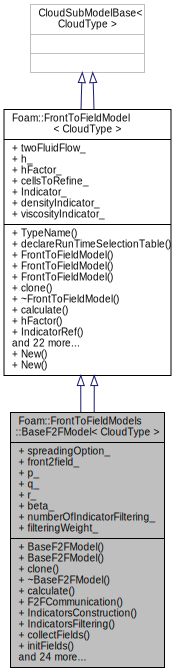
\includegraphics[height=550pt]{classFoam_1_1FrontToFieldModels_1_1BaseF2FModel__coll__graph}
\end{center}
\end{figure}
\subsection*{Public Types}
\begin{DoxyCompactItemize}
\item 
enum \hyperlink{classFoam_1_1FrontToFieldModels_1_1BaseF2FModel_a16ac12059f9cdbf69d5bef5029e9e2f3}{spreading\+Option} \{ \newline
\hyperlink{classFoam_1_1FrontToFieldModels_1_1BaseF2FModel_a16ac12059f9cdbf69d5bef5029e9e2f3a907dde658abcaa772bc8f12c725d72c0}{fixed}, 
\hyperlink{classFoam_1_1FrontToFieldModels_1_1BaseF2FModel_a16ac12059f9cdbf69d5bef5029e9e2f3acc1d4117a3f2af7a5be3465e2663cc57}{bubble\+Local}, 
\hyperlink{classFoam_1_1FrontToFieldModels_1_1BaseF2FModel_a16ac12059f9cdbf69d5bef5029e9e2f3ad2b751c9e2869ad95d2ddd6a4c02d5a1}{grid\+Local}, 
\hyperlink{classFoam_1_1FrontToFieldModels_1_1BaseF2FModel_a16ac12059f9cdbf69d5bef5029e9e2f3a907dde658abcaa772bc8f12c725d72c0}{fixed}, 
\newline
\hyperlink{classFoam_1_1FrontToFieldModels_1_1BaseF2FModel_a16ac12059f9cdbf69d5bef5029e9e2f3acc1d4117a3f2af7a5be3465e2663cc57}{bubble\+Local}, 
\hyperlink{classFoam_1_1FrontToFieldModels_1_1BaseF2FModel_a16ac12059f9cdbf69d5bef5029e9e2f3ad2b751c9e2869ad95d2ddd6a4c02d5a1}{grid\+Local}
 \}
\item 
enum \hyperlink{classFoam_1_1FrontToFieldModels_1_1BaseF2FModel_a16ac12059f9cdbf69d5bef5029e9e2f3}{spreading\+Option} \{ \newline
\hyperlink{classFoam_1_1FrontToFieldModels_1_1BaseF2FModel_a16ac12059f9cdbf69d5bef5029e9e2f3a907dde658abcaa772bc8f12c725d72c0}{fixed}, 
\hyperlink{classFoam_1_1FrontToFieldModels_1_1BaseF2FModel_a16ac12059f9cdbf69d5bef5029e9e2f3acc1d4117a3f2af7a5be3465e2663cc57}{bubble\+Local}, 
\hyperlink{classFoam_1_1FrontToFieldModels_1_1BaseF2FModel_a16ac12059f9cdbf69d5bef5029e9e2f3ad2b751c9e2869ad95d2ddd6a4c02d5a1}{grid\+Local}, 
\hyperlink{classFoam_1_1FrontToFieldModels_1_1BaseF2FModel_a16ac12059f9cdbf69d5bef5029e9e2f3a907dde658abcaa772bc8f12c725d72c0}{fixed}, 
\newline
\hyperlink{classFoam_1_1FrontToFieldModels_1_1BaseF2FModel_a16ac12059f9cdbf69d5bef5029e9e2f3acc1d4117a3f2af7a5be3465e2663cc57}{bubble\+Local}, 
\hyperlink{classFoam_1_1FrontToFieldModels_1_1BaseF2FModel_a16ac12059f9cdbf69d5bef5029e9e2f3ad2b751c9e2869ad95d2ddd6a4c02d5a1}{grid\+Local}
 \}
\end{DoxyCompactItemize}
\subsection*{Public Member Functions}
\begin{DoxyCompactItemize}
\item 
\hyperlink{classFoam_1_1FrontToFieldModels_1_1BaseF2FModel_ac56ffd97cb3476829542ba8393328484}{Base\+F2\+F\+Model} (const dictionary \&dict, Cloud\+Type \&owner, const word \&model\+Name)
\item 
\hyperlink{classFoam_1_1FrontToFieldModels_1_1BaseF2FModel_a1f186e44f430e10ac6b66e8990a7e529}{Base\+F2\+F\+Model} (const \hyperlink{classFoam_1_1FrontToFieldModels_1_1BaseF2FModel}{Base\+F2\+F\+Model}$<$ Cloud\+Type $>$ \&cm)
\item 
virtual auto\+Ptr$<$ \hyperlink{classFoam_1_1FrontToFieldModel}{Front\+To\+Field\+Model}$<$ Cloud\+Type $>$ $>$ \hyperlink{classFoam_1_1FrontToFieldModels_1_1BaseF2FModel_a28a0e5110316e77393efe30b9f243b08}{clone} () const =0
\item 
virtual \hyperlink{classFoam_1_1FrontToFieldModels_1_1BaseF2FModel_a2945be87ac5492a867f01c7fe54cc744}{$\sim$\+Base\+F2\+F\+Model} ()
\item 
virtual void \hyperlink{classFoam_1_1FrontToFieldModels_1_1BaseF2FModel_a1fd66572a83b6ec47ac9c2fb86064f19}{calculate} ()
\item 
virtual void \hyperlink{classFoam_1_1FrontToFieldModels_1_1BaseF2FModel_a4e17f34f93d0da473f4a601133bf10ce}{F2\+F\+Communication} ()
\item 
virtual void \hyperlink{classFoam_1_1FrontToFieldModels_1_1BaseF2FModel_a194c0c309124ae1cfcd5bf07b3d3528e}{Indicators\+Construction} ()=0
\item 
virtual void \hyperlink{classFoam_1_1FrontToFieldModels_1_1BaseF2FModel_aaf7d29f76d66eae9af2b303f8260167e}{Indicators\+Filtering} ()
\item 
virtual void \hyperlink{classFoam_1_1FrontToFieldModels_1_1BaseF2FModel_a22b3c4bb9f2660656b958208684ac9f8}{collect\+Fields} (label cellI, label b\+DI, scalar w\+Bar, vector el\+Area\+Vec)=0
\item 
virtual void \hyperlink{classFoam_1_1FrontToFieldModels_1_1BaseF2FModel_af404778ce26acab686dd1184da5749c5}{init\+Fields} ()=0
\item 
void \hyperlink{classFoam_1_1FrontToFieldModels_1_1BaseF2FModel_ab5821f5d89b402eaa3859c7879da4de1}{adjusting\+The\+Important\+Vars\+For\+Indicators} ()
\item 
scalar \hyperlink{classFoam_1_1FrontToFieldModels_1_1BaseF2FModel_a95285ac734272e03f6b69727db06a2c5}{bubble\+Hl} (label b\+DI)
\item 
scalar \hyperlink{classFoam_1_1FrontToFieldModels_1_1BaseF2FModel_a1d1e01607afc846240ff156850e9da36}{PeskinD} (scalar r, scalar h)
\item 
scalar \hyperlink{classFoam_1_1FrontToFieldModels_1_1BaseF2FModel_a022f033f51b4ddb89082282d4e92ae9f}{window\+Func} (vector del, scalar h)
\item 
scalar \hyperlink{classFoam_1_1FrontToFieldModels_1_1BaseF2FModel_af004d7b781e7e2a176b1ece4aee02a81}{window\+Func\+Bar} (vector del, scalar h, List$<$ scalar $>$ beta)
\item 
scalar \hyperlink{classFoam_1_1FrontToFieldModels_1_1BaseF2FModel_abd3be11e7be0d82ed00f201a8b1ea48c}{m\+P\+QR} (vector del, scalar h, label p, label q, label r)
\item 
scalar \hyperlink{classFoam_1_1FrontToFieldModels_1_1BaseF2FModel_aa31e5f4538c17f43cb00f5885816b518}{Liu\+Heviside} (scalar outer\+Fluid\+Property, scalar property, vector min\+Distance, vector element\+Surface\+Area, scalar gama)
\item 
\hyperlink{classFoam_1_1FrontToFieldModels_1_1BaseF2FModel_ac56ffd97cb3476829542ba8393328484}{Base\+F2\+F\+Model} (const dictionary \&dict, Cloud\+Type \&owner, const word \&model\+Name)
\item 
\hyperlink{classFoam_1_1FrontToFieldModels_1_1BaseF2FModel_a1f186e44f430e10ac6b66e8990a7e529}{Base\+F2\+F\+Model} (const \hyperlink{classFoam_1_1FrontToFieldModels_1_1BaseF2FModel}{Base\+F2\+F\+Model}$<$ Cloud\+Type $>$ \&cm)
\item 
virtual auto\+Ptr$<$ \hyperlink{classFoam_1_1FrontToFieldModel}{Front\+To\+Field\+Model}$<$ Cloud\+Type $>$ $>$ \hyperlink{classFoam_1_1FrontToFieldModels_1_1BaseF2FModel_a28a0e5110316e77393efe30b9f243b08}{clone} () const =0
\item 
virtual \hyperlink{classFoam_1_1FrontToFieldModels_1_1BaseF2FModel_a201bd44e36e0cc6949af85cff88d4fa5}{$\sim$\+Base\+F2\+F\+Model} ()
\item 
virtual void \hyperlink{classFoam_1_1FrontToFieldModels_1_1BaseF2FModel_a9417a2284bfa038e22a927d5c8e7d54b}{calculate} ()
\item 
virtual void \hyperlink{classFoam_1_1FrontToFieldModels_1_1BaseF2FModel_a6a9dcaabfbb5169748334511f5bef8f0}{F2\+F\+Communication} ()
\item 
virtual void \hyperlink{classFoam_1_1FrontToFieldModels_1_1BaseF2FModel_a194c0c309124ae1cfcd5bf07b3d3528e}{Indicators\+Construction} ()=0
\item 
virtual void \hyperlink{classFoam_1_1FrontToFieldModels_1_1BaseF2FModel_a94f5e4adf91b14b089978334d4a3b794}{Indicators\+Filtering} ()
\item 
virtual void \hyperlink{classFoam_1_1FrontToFieldModels_1_1BaseF2FModel_a22b3c4bb9f2660656b958208684ac9f8}{collect\+Fields} (label cellI, label b\+DI, scalar w\+Bar, vector el\+Area\+Vec)=0
\item 
virtual void \hyperlink{classFoam_1_1FrontToFieldModels_1_1BaseF2FModel_af404778ce26acab686dd1184da5749c5}{init\+Fields} ()=0
\item 
void \hyperlink{classFoam_1_1FrontToFieldModels_1_1BaseF2FModel_ab5821f5d89b402eaa3859c7879da4de1}{adjusting\+The\+Important\+Vars\+For\+Indicators} ()
\item 
scalar \hyperlink{classFoam_1_1FrontToFieldModels_1_1BaseF2FModel_adc46762e1cb49313cb9d8e3d1f720d94}{bubble\+Hl} (label b\+DI)
\item 
scalar \hyperlink{classFoam_1_1FrontToFieldModels_1_1BaseF2FModel_a8eaf0fc148f9a76dc85116567f12b3ce}{PeskinD} (scalar r, scalar h)
\item 
scalar \hyperlink{classFoam_1_1FrontToFieldModels_1_1BaseF2FModel_a25864f279b675ee9ba440f5d9b874b46}{window\+Func} (vector del, scalar h)
\item 
scalar \hyperlink{classFoam_1_1FrontToFieldModels_1_1BaseF2FModel_ab75791ed7cb3eb23ffa0cc29d464b7cc}{window\+Func\+Bar} (vector del, scalar h, List$<$ scalar $>$ beta)
\item 
scalar \hyperlink{classFoam_1_1FrontToFieldModels_1_1BaseF2FModel_a1c6fcd79305e088eb8a66ce91307bc70}{m\+P\+QR} (vector del, scalar h, label p, label q, label r)
\item 
scalar \hyperlink{classFoam_1_1FrontToFieldModels_1_1BaseF2FModel_a4152e84948cc7bbb273bc96da50c97ba}{Liu\+Heviside} (scalar outer\+Fluid\+Property, scalar property, vector min\+Distance, vector element\+Surface\+Area, scalar gama)
\end{DoxyCompactItemize}
\subsection*{Public Attributes}
\begin{DoxyCompactItemize}
\item 
\hyperlink{classFoam_1_1FrontToFieldModels_1_1BaseF2FModel_a16ac12059f9cdbf69d5bef5029e9e2f3}{spreading\+Option} \hyperlink{classFoam_1_1FrontToFieldModels_1_1BaseF2FModel_ac944d075a159992d2e38d2d9c0eb5c2e}{spreading\+Option\+\_\+}
\item 
word \hyperlink{classFoam_1_1FrontToFieldModels_1_1BaseF2FModel_a0e777bd8fd5a92cc3e9a8833a53be8a3}{front2field\+\_\+}
\item 
List$<$ label $>$ \hyperlink{classFoam_1_1FrontToFieldModels_1_1BaseF2FModel_a55b6ed327c5b3b4360d4a4f537a5e41e}{p\+\_\+}
\item 
List$<$ label $>$ \hyperlink{classFoam_1_1FrontToFieldModels_1_1BaseF2FModel_ae2f7cdcbcd60d5a849afc352765cdefe}{q\+\_\+}
\item 
List$<$ label $>$ \hyperlink{classFoam_1_1FrontToFieldModels_1_1BaseF2FModel_a2f335eed9c03847c9a84ad4d8d3bfa98}{r\+\_\+}
\item 
List$<$ scalar $>$ \hyperlink{classFoam_1_1FrontToFieldModels_1_1BaseF2FModel_a28af8ea6a018505dfd6618cbfe8d4a31}{beta\+\_\+}
\item 
label \hyperlink{classFoam_1_1FrontToFieldModels_1_1BaseF2FModel_a72b788105fc00ea41d1b1be73e18e6a2}{number\+Of\+Indicator\+Filtering\+\_\+} = 0
\item 
scalar \hyperlink{classFoam_1_1FrontToFieldModels_1_1BaseF2FModel_a1bcf6f9b3c688869536482e9ac76eda3}{filtering\+Weight\+\_\+} = 0.\+0
\end{DoxyCompactItemize}
\subsection*{Additional Inherited Members}


\subsection{Member Enumeration Documentation}
\mbox{\Hypertarget{classFoam_1_1FrontToFieldModels_1_1BaseF2FModel_a16ac12059f9cdbf69d5bef5029e9e2f3}\label{classFoam_1_1FrontToFieldModels_1_1BaseF2FModel_a16ac12059f9cdbf69d5bef5029e9e2f3}} 
\index{Foam\+::\+Front\+To\+Field\+Models\+::\+Base\+F2\+F\+Model@{Foam\+::\+Front\+To\+Field\+Models\+::\+Base\+F2\+F\+Model}!spreading\+Option@{spreading\+Option}}
\index{spreading\+Option@{spreading\+Option}!Foam\+::\+Front\+To\+Field\+Models\+::\+Base\+F2\+F\+Model@{Foam\+::\+Front\+To\+Field\+Models\+::\+Base\+F2\+F\+Model}}
\subsubsection{\texorpdfstring{spreading\+Option}{spreadingOption}\hspace{0.1cm}{\footnotesize\ttfamily [1/2]}}
{\footnotesize\ttfamily template$<$class Cloud\+Type$>$ \\
enum \hyperlink{classFoam_1_1FrontToFieldModels_1_1BaseF2FModel_a16ac12059f9cdbf69d5bef5029e9e2f3}{Foam\+::\+Front\+To\+Field\+Models\+::\+Base\+F2\+F\+Model\+::spreading\+Option}}

\begin{DoxyEnumFields}{Enumerator}
\raisebox{\heightof{T}}[0pt][0pt]{\index{fixed@{fixed}!Foam\+::\+Front\+To\+Field\+Models\+::\+Base\+F2\+F\+Model@{Foam\+::\+Front\+To\+Field\+Models\+::\+Base\+F2\+F\+Model}}\index{Foam\+::\+Front\+To\+Field\+Models\+::\+Base\+F2\+F\+Model@{Foam\+::\+Front\+To\+Field\+Models\+::\+Base\+F2\+F\+Model}!fixed@{fixed}}}\mbox{\Hypertarget{classFoam_1_1FrontToFieldModels_1_1BaseF2FModel_a16ac12059f9cdbf69d5bef5029e9e2f3a907dde658abcaa772bc8f12c725d72c0}\label{classFoam_1_1FrontToFieldModels_1_1BaseF2FModel_a16ac12059f9cdbf69d5bef5029e9e2f3a907dde658abcaa772bc8f12c725d72c0}} 
fixed&\\
\hline

\raisebox{\heightof{T}}[0pt][0pt]{\index{bubble\+Local@{bubble\+Local}!Foam\+::\+Front\+To\+Field\+Models\+::\+Base\+F2\+F\+Model@{Foam\+::\+Front\+To\+Field\+Models\+::\+Base\+F2\+F\+Model}}\index{Foam\+::\+Front\+To\+Field\+Models\+::\+Base\+F2\+F\+Model@{Foam\+::\+Front\+To\+Field\+Models\+::\+Base\+F2\+F\+Model}!bubble\+Local@{bubble\+Local}}}\mbox{\Hypertarget{classFoam_1_1FrontToFieldModels_1_1BaseF2FModel_a16ac12059f9cdbf69d5bef5029e9e2f3acc1d4117a3f2af7a5be3465e2663cc57}\label{classFoam_1_1FrontToFieldModels_1_1BaseF2FModel_a16ac12059f9cdbf69d5bef5029e9e2f3acc1d4117a3f2af7a5be3465e2663cc57}} 
bubble\+Local&\\
\hline

\raisebox{\heightof{T}}[0pt][0pt]{\index{grid\+Local@{grid\+Local}!Foam\+::\+Front\+To\+Field\+Models\+::\+Base\+F2\+F\+Model@{Foam\+::\+Front\+To\+Field\+Models\+::\+Base\+F2\+F\+Model}}\index{Foam\+::\+Front\+To\+Field\+Models\+::\+Base\+F2\+F\+Model@{Foam\+::\+Front\+To\+Field\+Models\+::\+Base\+F2\+F\+Model}!grid\+Local@{grid\+Local}}}\mbox{\Hypertarget{classFoam_1_1FrontToFieldModels_1_1BaseF2FModel_a16ac12059f9cdbf69d5bef5029e9e2f3ad2b751c9e2869ad95d2ddd6a4c02d5a1}\label{classFoam_1_1FrontToFieldModels_1_1BaseF2FModel_a16ac12059f9cdbf69d5bef5029e9e2f3ad2b751c9e2869ad95d2ddd6a4c02d5a1}} 
grid\+Local&\\
\hline

\raisebox{\heightof{T}}[0pt][0pt]{\index{fixed@{fixed}!Foam\+::\+Front\+To\+Field\+Models\+::\+Base\+F2\+F\+Model@{Foam\+::\+Front\+To\+Field\+Models\+::\+Base\+F2\+F\+Model}}\index{Foam\+::\+Front\+To\+Field\+Models\+::\+Base\+F2\+F\+Model@{Foam\+::\+Front\+To\+Field\+Models\+::\+Base\+F2\+F\+Model}!fixed@{fixed}}}\mbox{\Hypertarget{classFoam_1_1FrontToFieldModels_1_1BaseF2FModel_a16ac12059f9cdbf69d5bef5029e9e2f3a907dde658abcaa772bc8f12c725d72c0}\label{classFoam_1_1FrontToFieldModels_1_1BaseF2FModel_a16ac12059f9cdbf69d5bef5029e9e2f3a907dde658abcaa772bc8f12c725d72c0}} 
fixed&\\
\hline

\raisebox{\heightof{T}}[0pt][0pt]{\index{bubble\+Local@{bubble\+Local}!Foam\+::\+Front\+To\+Field\+Models\+::\+Base\+F2\+F\+Model@{Foam\+::\+Front\+To\+Field\+Models\+::\+Base\+F2\+F\+Model}}\index{Foam\+::\+Front\+To\+Field\+Models\+::\+Base\+F2\+F\+Model@{Foam\+::\+Front\+To\+Field\+Models\+::\+Base\+F2\+F\+Model}!bubble\+Local@{bubble\+Local}}}\mbox{\Hypertarget{classFoam_1_1FrontToFieldModels_1_1BaseF2FModel_a16ac12059f9cdbf69d5bef5029e9e2f3acc1d4117a3f2af7a5be3465e2663cc57}\label{classFoam_1_1FrontToFieldModels_1_1BaseF2FModel_a16ac12059f9cdbf69d5bef5029e9e2f3acc1d4117a3f2af7a5be3465e2663cc57}} 
bubble\+Local&\\
\hline

\raisebox{\heightof{T}}[0pt][0pt]{\index{grid\+Local@{grid\+Local}!Foam\+::\+Front\+To\+Field\+Models\+::\+Base\+F2\+F\+Model@{Foam\+::\+Front\+To\+Field\+Models\+::\+Base\+F2\+F\+Model}}\index{Foam\+::\+Front\+To\+Field\+Models\+::\+Base\+F2\+F\+Model@{Foam\+::\+Front\+To\+Field\+Models\+::\+Base\+F2\+F\+Model}!grid\+Local@{grid\+Local}}}\mbox{\Hypertarget{classFoam_1_1FrontToFieldModels_1_1BaseF2FModel_a16ac12059f9cdbf69d5bef5029e9e2f3ad2b751c9e2869ad95d2ddd6a4c02d5a1}\label{classFoam_1_1FrontToFieldModels_1_1BaseF2FModel_a16ac12059f9cdbf69d5bef5029e9e2f3ad2b751c9e2869ad95d2ddd6a4c02d5a1}} 
grid\+Local&\\
\hline

\end{DoxyEnumFields}
\mbox{\Hypertarget{classFoam_1_1FrontToFieldModels_1_1BaseF2FModel_a16ac12059f9cdbf69d5bef5029e9e2f3}\label{classFoam_1_1FrontToFieldModels_1_1BaseF2FModel_a16ac12059f9cdbf69d5bef5029e9e2f3}} 
\index{Foam\+::\+Front\+To\+Field\+Models\+::\+Base\+F2\+F\+Model@{Foam\+::\+Front\+To\+Field\+Models\+::\+Base\+F2\+F\+Model}!spreading\+Option@{spreading\+Option}}
\index{spreading\+Option@{spreading\+Option}!Foam\+::\+Front\+To\+Field\+Models\+::\+Base\+F2\+F\+Model@{Foam\+::\+Front\+To\+Field\+Models\+::\+Base\+F2\+F\+Model}}
\subsubsection{\texorpdfstring{spreading\+Option}{spreadingOption}\hspace{0.1cm}{\footnotesize\ttfamily [2/2]}}
{\footnotesize\ttfamily template$<$class Cloud\+Type$>$ \\
enum \hyperlink{classFoam_1_1FrontToFieldModels_1_1BaseF2FModel_a16ac12059f9cdbf69d5bef5029e9e2f3}{Foam\+::\+Front\+To\+Field\+Models\+::\+Base\+F2\+F\+Model\+::spreading\+Option}}

\begin{DoxyEnumFields}{Enumerator}
\raisebox{\heightof{T}}[0pt][0pt]{\index{fixed@{fixed}!Foam\+::\+Front\+To\+Field\+Models\+::\+Base\+F2\+F\+Model@{Foam\+::\+Front\+To\+Field\+Models\+::\+Base\+F2\+F\+Model}}\index{Foam\+::\+Front\+To\+Field\+Models\+::\+Base\+F2\+F\+Model@{Foam\+::\+Front\+To\+Field\+Models\+::\+Base\+F2\+F\+Model}!fixed@{fixed}}}\mbox{\Hypertarget{classFoam_1_1FrontToFieldModels_1_1BaseF2FModel_a16ac12059f9cdbf69d5bef5029e9e2f3a907dde658abcaa772bc8f12c725d72c0}\label{classFoam_1_1FrontToFieldModels_1_1BaseF2FModel_a16ac12059f9cdbf69d5bef5029e9e2f3a907dde658abcaa772bc8f12c725d72c0}} 
fixed&\\
\hline

\raisebox{\heightof{T}}[0pt][0pt]{\index{bubble\+Local@{bubble\+Local}!Foam\+::\+Front\+To\+Field\+Models\+::\+Base\+F2\+F\+Model@{Foam\+::\+Front\+To\+Field\+Models\+::\+Base\+F2\+F\+Model}}\index{Foam\+::\+Front\+To\+Field\+Models\+::\+Base\+F2\+F\+Model@{Foam\+::\+Front\+To\+Field\+Models\+::\+Base\+F2\+F\+Model}!bubble\+Local@{bubble\+Local}}}\mbox{\Hypertarget{classFoam_1_1FrontToFieldModels_1_1BaseF2FModel_a16ac12059f9cdbf69d5bef5029e9e2f3acc1d4117a3f2af7a5be3465e2663cc57}\label{classFoam_1_1FrontToFieldModels_1_1BaseF2FModel_a16ac12059f9cdbf69d5bef5029e9e2f3acc1d4117a3f2af7a5be3465e2663cc57}} 
bubble\+Local&\\
\hline

\raisebox{\heightof{T}}[0pt][0pt]{\index{grid\+Local@{grid\+Local}!Foam\+::\+Front\+To\+Field\+Models\+::\+Base\+F2\+F\+Model@{Foam\+::\+Front\+To\+Field\+Models\+::\+Base\+F2\+F\+Model}}\index{Foam\+::\+Front\+To\+Field\+Models\+::\+Base\+F2\+F\+Model@{Foam\+::\+Front\+To\+Field\+Models\+::\+Base\+F2\+F\+Model}!grid\+Local@{grid\+Local}}}\mbox{\Hypertarget{classFoam_1_1FrontToFieldModels_1_1BaseF2FModel_a16ac12059f9cdbf69d5bef5029e9e2f3ad2b751c9e2869ad95d2ddd6a4c02d5a1}\label{classFoam_1_1FrontToFieldModels_1_1BaseF2FModel_a16ac12059f9cdbf69d5bef5029e9e2f3ad2b751c9e2869ad95d2ddd6a4c02d5a1}} 
grid\+Local&\\
\hline

\raisebox{\heightof{T}}[0pt][0pt]{\index{fixed@{fixed}!Foam\+::\+Front\+To\+Field\+Models\+::\+Base\+F2\+F\+Model@{Foam\+::\+Front\+To\+Field\+Models\+::\+Base\+F2\+F\+Model}}\index{Foam\+::\+Front\+To\+Field\+Models\+::\+Base\+F2\+F\+Model@{Foam\+::\+Front\+To\+Field\+Models\+::\+Base\+F2\+F\+Model}!fixed@{fixed}}}\mbox{\Hypertarget{classFoam_1_1FrontToFieldModels_1_1BaseF2FModel_a16ac12059f9cdbf69d5bef5029e9e2f3a907dde658abcaa772bc8f12c725d72c0}\label{classFoam_1_1FrontToFieldModels_1_1BaseF2FModel_a16ac12059f9cdbf69d5bef5029e9e2f3a907dde658abcaa772bc8f12c725d72c0}} 
fixed&\\
\hline

\raisebox{\heightof{T}}[0pt][0pt]{\index{bubble\+Local@{bubble\+Local}!Foam\+::\+Front\+To\+Field\+Models\+::\+Base\+F2\+F\+Model@{Foam\+::\+Front\+To\+Field\+Models\+::\+Base\+F2\+F\+Model}}\index{Foam\+::\+Front\+To\+Field\+Models\+::\+Base\+F2\+F\+Model@{Foam\+::\+Front\+To\+Field\+Models\+::\+Base\+F2\+F\+Model}!bubble\+Local@{bubble\+Local}}}\mbox{\Hypertarget{classFoam_1_1FrontToFieldModels_1_1BaseF2FModel_a16ac12059f9cdbf69d5bef5029e9e2f3acc1d4117a3f2af7a5be3465e2663cc57}\label{classFoam_1_1FrontToFieldModels_1_1BaseF2FModel_a16ac12059f9cdbf69d5bef5029e9e2f3acc1d4117a3f2af7a5be3465e2663cc57}} 
bubble\+Local&\\
\hline

\raisebox{\heightof{T}}[0pt][0pt]{\index{grid\+Local@{grid\+Local}!Foam\+::\+Front\+To\+Field\+Models\+::\+Base\+F2\+F\+Model@{Foam\+::\+Front\+To\+Field\+Models\+::\+Base\+F2\+F\+Model}}\index{Foam\+::\+Front\+To\+Field\+Models\+::\+Base\+F2\+F\+Model@{Foam\+::\+Front\+To\+Field\+Models\+::\+Base\+F2\+F\+Model}!grid\+Local@{grid\+Local}}}\mbox{\Hypertarget{classFoam_1_1FrontToFieldModels_1_1BaseF2FModel_a16ac12059f9cdbf69d5bef5029e9e2f3ad2b751c9e2869ad95d2ddd6a4c02d5a1}\label{classFoam_1_1FrontToFieldModels_1_1BaseF2FModel_a16ac12059f9cdbf69d5bef5029e9e2f3ad2b751c9e2869ad95d2ddd6a4c02d5a1}} 
grid\+Local&\\
\hline

\end{DoxyEnumFields}


\subsection{Constructor \& Destructor Documentation}
\mbox{\Hypertarget{classFoam_1_1FrontToFieldModels_1_1BaseF2FModel_ac56ffd97cb3476829542ba8393328484}\label{classFoam_1_1FrontToFieldModels_1_1BaseF2FModel_ac56ffd97cb3476829542ba8393328484}} 
\index{Foam\+::\+Front\+To\+Field\+Models\+::\+Base\+F2\+F\+Model@{Foam\+::\+Front\+To\+Field\+Models\+::\+Base\+F2\+F\+Model}!Base\+F2\+F\+Model@{Base\+F2\+F\+Model}}
\index{Base\+F2\+F\+Model@{Base\+F2\+F\+Model}!Foam\+::\+Front\+To\+Field\+Models\+::\+Base\+F2\+F\+Model@{Foam\+::\+Front\+To\+Field\+Models\+::\+Base\+F2\+F\+Model}}
\subsubsection{\texorpdfstring{Base\+F2\+F\+Model()}{BaseF2FModel()}\hspace{0.1cm}{\footnotesize\ttfamily [1/4]}}
{\footnotesize\ttfamily template$<$class Cloud\+Type $>$ \\
\hyperlink{classFoam_1_1FrontToFieldModels_1_1BaseF2FModel}{Foam\+::\+Front\+To\+Field\+Models\+::\+Base\+F2\+F\+Model}$<$ Cloud\+Type $>$\+::\hyperlink{classFoam_1_1FrontToFieldModels_1_1BaseF2FModel}{Base\+F2\+F\+Model} (\begin{DoxyParamCaption}\item[{const dictionary \&}]{dict,  }\item[{Cloud\+Type \&}]{owner,  }\item[{const word \&}]{model\+Name }\end{DoxyParamCaption})}

\mbox{\Hypertarget{classFoam_1_1FrontToFieldModels_1_1BaseF2FModel_a1f186e44f430e10ac6b66e8990a7e529}\label{classFoam_1_1FrontToFieldModels_1_1BaseF2FModel_a1f186e44f430e10ac6b66e8990a7e529}} 
\index{Foam\+::\+Front\+To\+Field\+Models\+::\+Base\+F2\+F\+Model@{Foam\+::\+Front\+To\+Field\+Models\+::\+Base\+F2\+F\+Model}!Base\+F2\+F\+Model@{Base\+F2\+F\+Model}}
\index{Base\+F2\+F\+Model@{Base\+F2\+F\+Model}!Foam\+::\+Front\+To\+Field\+Models\+::\+Base\+F2\+F\+Model@{Foam\+::\+Front\+To\+Field\+Models\+::\+Base\+F2\+F\+Model}}
\subsubsection{\texorpdfstring{Base\+F2\+F\+Model()}{BaseF2FModel()}\hspace{0.1cm}{\footnotesize\ttfamily [2/4]}}
{\footnotesize\ttfamily template$<$class Cloud\+Type $>$ \\
\hyperlink{classFoam_1_1FrontToFieldModels_1_1BaseF2FModel}{Foam\+::\+Front\+To\+Field\+Models\+::\+Base\+F2\+F\+Model}$<$ Cloud\+Type $>$\+::\hyperlink{classFoam_1_1FrontToFieldModels_1_1BaseF2FModel}{Base\+F2\+F\+Model} (\begin{DoxyParamCaption}\item[{const \hyperlink{classFoam_1_1FrontToFieldModels_1_1BaseF2FModel}{Base\+F2\+F\+Model}$<$ Cloud\+Type $>$ \&}]{cm }\end{DoxyParamCaption})}

\mbox{\Hypertarget{classFoam_1_1FrontToFieldModels_1_1BaseF2FModel_a2945be87ac5492a867f01c7fe54cc744}\label{classFoam_1_1FrontToFieldModels_1_1BaseF2FModel_a2945be87ac5492a867f01c7fe54cc744}} 
\index{Foam\+::\+Front\+To\+Field\+Models\+::\+Base\+F2\+F\+Model@{Foam\+::\+Front\+To\+Field\+Models\+::\+Base\+F2\+F\+Model}!````~Base\+F2\+F\+Model@{$\sim$\+Base\+F2\+F\+Model}}
\index{````~Base\+F2\+F\+Model@{$\sim$\+Base\+F2\+F\+Model}!Foam\+::\+Front\+To\+Field\+Models\+::\+Base\+F2\+F\+Model@{Foam\+::\+Front\+To\+Field\+Models\+::\+Base\+F2\+F\+Model}}
\subsubsection{\texorpdfstring{$\sim$\+Base\+F2\+F\+Model()}{~BaseF2FModel()}\hspace{0.1cm}{\footnotesize\ttfamily [1/2]}}
{\footnotesize\ttfamily template$<$class Cloud\+Type $>$ \\
\hyperlink{classFoam_1_1FrontToFieldModels_1_1BaseF2FModel}{Foam\+::\+Front\+To\+Field\+Models\+::\+Base\+F2\+F\+Model}$<$ Cloud\+Type $>$\+::$\sim$\hyperlink{classFoam_1_1FrontToFieldModels_1_1BaseF2FModel}{Base\+F2\+F\+Model} (\begin{DoxyParamCaption}{ }\end{DoxyParamCaption})\hspace{0.3cm}{\ttfamily [virtual]}}

\mbox{\Hypertarget{classFoam_1_1FrontToFieldModels_1_1BaseF2FModel_ac56ffd97cb3476829542ba8393328484}\label{classFoam_1_1FrontToFieldModels_1_1BaseF2FModel_ac56ffd97cb3476829542ba8393328484}} 
\index{Foam\+::\+Front\+To\+Field\+Models\+::\+Base\+F2\+F\+Model@{Foam\+::\+Front\+To\+Field\+Models\+::\+Base\+F2\+F\+Model}!Base\+F2\+F\+Model@{Base\+F2\+F\+Model}}
\index{Base\+F2\+F\+Model@{Base\+F2\+F\+Model}!Foam\+::\+Front\+To\+Field\+Models\+::\+Base\+F2\+F\+Model@{Foam\+::\+Front\+To\+Field\+Models\+::\+Base\+F2\+F\+Model}}
\subsubsection{\texorpdfstring{Base\+F2\+F\+Model()}{BaseF2FModel()}\hspace{0.1cm}{\footnotesize\ttfamily [3/4]}}
{\footnotesize\ttfamily template$<$class Cloud\+Type$>$ \\
\hyperlink{classFoam_1_1FrontToFieldModels_1_1BaseF2FModel}{Foam\+::\+Front\+To\+Field\+Models\+::\+Base\+F2\+F\+Model}$<$ Cloud\+Type $>$\+::\hyperlink{classFoam_1_1FrontToFieldModels_1_1BaseF2FModel}{Base\+F2\+F\+Model} (\begin{DoxyParamCaption}\item[{const dictionary \&}]{dict,  }\item[{Cloud\+Type \&}]{owner,  }\item[{const word \&}]{model\+Name }\end{DoxyParamCaption})}

\mbox{\Hypertarget{classFoam_1_1FrontToFieldModels_1_1BaseF2FModel_a1f186e44f430e10ac6b66e8990a7e529}\label{classFoam_1_1FrontToFieldModels_1_1BaseF2FModel_a1f186e44f430e10ac6b66e8990a7e529}} 
\index{Foam\+::\+Front\+To\+Field\+Models\+::\+Base\+F2\+F\+Model@{Foam\+::\+Front\+To\+Field\+Models\+::\+Base\+F2\+F\+Model}!Base\+F2\+F\+Model@{Base\+F2\+F\+Model}}
\index{Base\+F2\+F\+Model@{Base\+F2\+F\+Model}!Foam\+::\+Front\+To\+Field\+Models\+::\+Base\+F2\+F\+Model@{Foam\+::\+Front\+To\+Field\+Models\+::\+Base\+F2\+F\+Model}}
\subsubsection{\texorpdfstring{Base\+F2\+F\+Model()}{BaseF2FModel()}\hspace{0.1cm}{\footnotesize\ttfamily [4/4]}}
{\footnotesize\ttfamily template$<$class Cloud\+Type$>$ \\
\hyperlink{classFoam_1_1FrontToFieldModels_1_1BaseF2FModel}{Foam\+::\+Front\+To\+Field\+Models\+::\+Base\+F2\+F\+Model}$<$ Cloud\+Type $>$\+::\hyperlink{classFoam_1_1FrontToFieldModels_1_1BaseF2FModel}{Base\+F2\+F\+Model} (\begin{DoxyParamCaption}\item[{const \hyperlink{classFoam_1_1FrontToFieldModels_1_1BaseF2FModel}{Base\+F2\+F\+Model}$<$ Cloud\+Type $>$ \&}]{cm }\end{DoxyParamCaption})}

\mbox{\Hypertarget{classFoam_1_1FrontToFieldModels_1_1BaseF2FModel_a201bd44e36e0cc6949af85cff88d4fa5}\label{classFoam_1_1FrontToFieldModels_1_1BaseF2FModel_a201bd44e36e0cc6949af85cff88d4fa5}} 
\index{Foam\+::\+Front\+To\+Field\+Models\+::\+Base\+F2\+F\+Model@{Foam\+::\+Front\+To\+Field\+Models\+::\+Base\+F2\+F\+Model}!````~Base\+F2\+F\+Model@{$\sim$\+Base\+F2\+F\+Model}}
\index{````~Base\+F2\+F\+Model@{$\sim$\+Base\+F2\+F\+Model}!Foam\+::\+Front\+To\+Field\+Models\+::\+Base\+F2\+F\+Model@{Foam\+::\+Front\+To\+Field\+Models\+::\+Base\+F2\+F\+Model}}
\subsubsection{\texorpdfstring{$\sim$\+Base\+F2\+F\+Model()}{~BaseF2FModel()}\hspace{0.1cm}{\footnotesize\ttfamily [2/2]}}
{\footnotesize\ttfamily template$<$class Cloud\+Type$>$ \\
virtual \hyperlink{classFoam_1_1FrontToFieldModels_1_1BaseF2FModel}{Foam\+::\+Front\+To\+Field\+Models\+::\+Base\+F2\+F\+Model}$<$ Cloud\+Type $>$\+::$\sim$\hyperlink{classFoam_1_1FrontToFieldModels_1_1BaseF2FModel}{Base\+F2\+F\+Model} (\begin{DoxyParamCaption}{ }\end{DoxyParamCaption})\hspace{0.3cm}{\ttfamily [virtual]}}



\subsection{Member Function Documentation}
\mbox{\Hypertarget{classFoam_1_1FrontToFieldModels_1_1BaseF2FModel_ab5821f5d89b402eaa3859c7879da4de1}\label{classFoam_1_1FrontToFieldModels_1_1BaseF2FModel_ab5821f5d89b402eaa3859c7879da4de1}} 
\index{Foam\+::\+Front\+To\+Field\+Models\+::\+Base\+F2\+F\+Model@{Foam\+::\+Front\+To\+Field\+Models\+::\+Base\+F2\+F\+Model}!adjusting\+The\+Important\+Vars\+For\+Indicators@{adjusting\+The\+Important\+Vars\+For\+Indicators}}
\index{adjusting\+The\+Important\+Vars\+For\+Indicators@{adjusting\+The\+Important\+Vars\+For\+Indicators}!Foam\+::\+Front\+To\+Field\+Models\+::\+Base\+F2\+F\+Model@{Foam\+::\+Front\+To\+Field\+Models\+::\+Base\+F2\+F\+Model}}
\subsubsection{\texorpdfstring{adjusting\+The\+Important\+Vars\+For\+Indicators()}{adjustingTheImportantVarsForIndicators()}\hspace{0.1cm}{\footnotesize\ttfamily [1/2]}}
{\footnotesize\ttfamily template$<$class Cloud\+Type $>$ \\
void \hyperlink{classFoam_1_1FrontToFieldModels_1_1BaseF2FModel}{Foam\+::\+Front\+To\+Field\+Models\+::\+Base\+F2\+F\+Model}$<$ Cloud\+Type $>$\+::adjusting\+The\+Important\+Vars\+For\+Indicators (\begin{DoxyParamCaption}{ }\end{DoxyParamCaption})\hspace{0.3cm}{\ttfamily [inline]}}

Here is the call graph for this function\+:\nopagebreak
\begin{figure}[H]
\begin{center}
\leavevmode
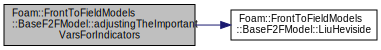
\includegraphics[width=350pt]{classFoam_1_1FrontToFieldModels_1_1BaseF2FModel_ab5821f5d89b402eaa3859c7879da4de1_cgraph}
\end{center}
\end{figure}
\mbox{\Hypertarget{classFoam_1_1FrontToFieldModels_1_1BaseF2FModel_ab5821f5d89b402eaa3859c7879da4de1}\label{classFoam_1_1FrontToFieldModels_1_1BaseF2FModel_ab5821f5d89b402eaa3859c7879da4de1}} 
\index{Foam\+::\+Front\+To\+Field\+Models\+::\+Base\+F2\+F\+Model@{Foam\+::\+Front\+To\+Field\+Models\+::\+Base\+F2\+F\+Model}!adjusting\+The\+Important\+Vars\+For\+Indicators@{adjusting\+The\+Important\+Vars\+For\+Indicators}}
\index{adjusting\+The\+Important\+Vars\+For\+Indicators@{adjusting\+The\+Important\+Vars\+For\+Indicators}!Foam\+::\+Front\+To\+Field\+Models\+::\+Base\+F2\+F\+Model@{Foam\+::\+Front\+To\+Field\+Models\+::\+Base\+F2\+F\+Model}}
\subsubsection{\texorpdfstring{adjusting\+The\+Important\+Vars\+For\+Indicators()}{adjustingTheImportantVarsForIndicators()}\hspace{0.1cm}{\footnotesize\ttfamily [2/2]}}
{\footnotesize\ttfamily template$<$class Cloud\+Type$>$ \\
void \hyperlink{classFoam_1_1FrontToFieldModels_1_1BaseF2FModel}{Foam\+::\+Front\+To\+Field\+Models\+::\+Base\+F2\+F\+Model}$<$ Cloud\+Type $>$\+::adjusting\+The\+Important\+Vars\+For\+Indicators (\begin{DoxyParamCaption}{ }\end{DoxyParamCaption})\hspace{0.3cm}{\ttfamily [inline]}}

\mbox{\Hypertarget{classFoam_1_1FrontToFieldModels_1_1BaseF2FModel_a95285ac734272e03f6b69727db06a2c5}\label{classFoam_1_1FrontToFieldModels_1_1BaseF2FModel_a95285ac734272e03f6b69727db06a2c5}} 
\index{Foam\+::\+Front\+To\+Field\+Models\+::\+Base\+F2\+F\+Model@{Foam\+::\+Front\+To\+Field\+Models\+::\+Base\+F2\+F\+Model}!bubble\+Hl@{bubble\+Hl}}
\index{bubble\+Hl@{bubble\+Hl}!Foam\+::\+Front\+To\+Field\+Models\+::\+Base\+F2\+F\+Model@{Foam\+::\+Front\+To\+Field\+Models\+::\+Base\+F2\+F\+Model}}
\subsubsection{\texorpdfstring{bubble\+Hl()}{bubbleHl()}\hspace{0.1cm}{\footnotesize\ttfamily [1/2]}}
{\footnotesize\ttfamily template$<$class Cloud\+Type $>$ \\
Foam\+::scalar \hyperlink{classFoam_1_1FrontToFieldModels_1_1BaseF2FModel}{Foam\+::\+Front\+To\+Field\+Models\+::\+Base\+F2\+F\+Model}$<$ Cloud\+Type $>$\+::bubble\+Hl (\begin{DoxyParamCaption}\item[{label}]{b\+DI }\end{DoxyParamCaption})\hspace{0.3cm}{\ttfamily [inline]}}

\mbox{\Hypertarget{classFoam_1_1FrontToFieldModels_1_1BaseF2FModel_adc46762e1cb49313cb9d8e3d1f720d94}\label{classFoam_1_1FrontToFieldModels_1_1BaseF2FModel_adc46762e1cb49313cb9d8e3d1f720d94}} 
\index{Foam\+::\+Front\+To\+Field\+Models\+::\+Base\+F2\+F\+Model@{Foam\+::\+Front\+To\+Field\+Models\+::\+Base\+F2\+F\+Model}!bubble\+Hl@{bubble\+Hl}}
\index{bubble\+Hl@{bubble\+Hl}!Foam\+::\+Front\+To\+Field\+Models\+::\+Base\+F2\+F\+Model@{Foam\+::\+Front\+To\+Field\+Models\+::\+Base\+F2\+F\+Model}}
\subsubsection{\texorpdfstring{bubble\+Hl()}{bubbleHl()}\hspace{0.1cm}{\footnotesize\ttfamily [2/2]}}
{\footnotesize\ttfamily template$<$class Cloud\+Type$>$ \\
scalar \hyperlink{classFoam_1_1FrontToFieldModels_1_1BaseF2FModel}{Foam\+::\+Front\+To\+Field\+Models\+::\+Base\+F2\+F\+Model}$<$ Cloud\+Type $>$\+::bubble\+Hl (\begin{DoxyParamCaption}\item[{label}]{b\+DI }\end{DoxyParamCaption})\hspace{0.3cm}{\ttfamily [inline]}}

\mbox{\Hypertarget{classFoam_1_1FrontToFieldModels_1_1BaseF2FModel_a1fd66572a83b6ec47ac9c2fb86064f19}\label{classFoam_1_1FrontToFieldModels_1_1BaseF2FModel_a1fd66572a83b6ec47ac9c2fb86064f19}} 
\index{Foam\+::\+Front\+To\+Field\+Models\+::\+Base\+F2\+F\+Model@{Foam\+::\+Front\+To\+Field\+Models\+::\+Base\+F2\+F\+Model}!calculate@{calculate}}
\index{calculate@{calculate}!Foam\+::\+Front\+To\+Field\+Models\+::\+Base\+F2\+F\+Model@{Foam\+::\+Front\+To\+Field\+Models\+::\+Base\+F2\+F\+Model}}
\subsubsection{\texorpdfstring{calculate()}{calculate()}\hspace{0.1cm}{\footnotesize\ttfamily [1/2]}}
{\footnotesize\ttfamily template$<$class Cloud\+Type $>$ \\
void \hyperlink{classFoam_1_1FrontToFieldModels_1_1BaseF2FModel}{Foam\+::\+Front\+To\+Field\+Models\+::\+Base\+F2\+F\+Model}$<$ Cloud\+Type $>$\+::calculate (\begin{DoxyParamCaption}{ }\end{DoxyParamCaption})\hspace{0.3cm}{\ttfamily [virtual]}}



Implements \hyperlink{classFoam_1_1FrontToFieldModel_a88ce933bcfddfcb36401aba9c0776ae5}{Foam\+::\+Front\+To\+Field\+Model$<$ Cloud\+Type $>$}.

\mbox{\Hypertarget{classFoam_1_1FrontToFieldModels_1_1BaseF2FModel_a9417a2284bfa038e22a927d5c8e7d54b}\label{classFoam_1_1FrontToFieldModels_1_1BaseF2FModel_a9417a2284bfa038e22a927d5c8e7d54b}} 
\index{Foam\+::\+Front\+To\+Field\+Models\+::\+Base\+F2\+F\+Model@{Foam\+::\+Front\+To\+Field\+Models\+::\+Base\+F2\+F\+Model}!calculate@{calculate}}
\index{calculate@{calculate}!Foam\+::\+Front\+To\+Field\+Models\+::\+Base\+F2\+F\+Model@{Foam\+::\+Front\+To\+Field\+Models\+::\+Base\+F2\+F\+Model}}
\subsubsection{\texorpdfstring{calculate()}{calculate()}\hspace{0.1cm}{\footnotesize\ttfamily [2/2]}}
{\footnotesize\ttfamily template$<$class Cloud\+Type$>$ \\
virtual void \hyperlink{classFoam_1_1FrontToFieldModels_1_1BaseF2FModel}{Foam\+::\+Front\+To\+Field\+Models\+::\+Base\+F2\+F\+Model}$<$ Cloud\+Type $>$\+::calculate (\begin{DoxyParamCaption}{ }\end{DoxyParamCaption})\hspace{0.3cm}{\ttfamily [virtual]}}



Implements \hyperlink{classFoam_1_1FrontToFieldModel_a88ce933bcfddfcb36401aba9c0776ae5}{Foam\+::\+Front\+To\+Field\+Model$<$ Cloud\+Type $>$}.

\mbox{\Hypertarget{classFoam_1_1FrontToFieldModels_1_1BaseF2FModel_a28a0e5110316e77393efe30b9f243b08}\label{classFoam_1_1FrontToFieldModels_1_1BaseF2FModel_a28a0e5110316e77393efe30b9f243b08}} 
\index{Foam\+::\+Front\+To\+Field\+Models\+::\+Base\+F2\+F\+Model@{Foam\+::\+Front\+To\+Field\+Models\+::\+Base\+F2\+F\+Model}!clone@{clone}}
\index{clone@{clone}!Foam\+::\+Front\+To\+Field\+Models\+::\+Base\+F2\+F\+Model@{Foam\+::\+Front\+To\+Field\+Models\+::\+Base\+F2\+F\+Model}}
\subsubsection{\texorpdfstring{clone()}{clone()}\hspace{0.1cm}{\footnotesize\ttfamily [1/2]}}
{\footnotesize\ttfamily template$<$class Cloud\+Type$>$ \\
virtual auto\+Ptr$<$\hyperlink{classFoam_1_1FrontToFieldModel}{Front\+To\+Field\+Model}$<$Cloud\+Type$>$ $>$ \hyperlink{classFoam_1_1FrontToFieldModels_1_1BaseF2FModel}{Foam\+::\+Front\+To\+Field\+Models\+::\+Base\+F2\+F\+Model}$<$ Cloud\+Type $>$\+::clone (\begin{DoxyParamCaption}{ }\end{DoxyParamCaption}) const\hspace{0.3cm}{\ttfamily [pure virtual]}}



Implements \hyperlink{classFoam_1_1FrontToFieldModel_a0c13ce2692d43dece9d9e51f6c0c5fd6}{Foam\+::\+Front\+To\+Field\+Model$<$ Cloud\+Type $>$}.



Implemented in \hyperlink{classFoam_1_1FrontToFieldModels_1_1CPT_a1ba03c46bac4bba07f9ee8185baff1e6}{Foam\+::\+Front\+To\+Field\+Models\+::\+C\+P\+T$<$ Cloud\+Type $>$}, \hyperlink{classFoam_1_1FrontToFieldModels_1_1CPT_a1ba03c46bac4bba07f9ee8185baff1e6}{Foam\+::\+Front\+To\+Field\+Models\+::\+C\+P\+T$<$ Cloud\+Type $>$}, \hyperlink{classFoam_1_1FrontToFieldModels_1_1Poisson_a2427c93360419e2494a682227ee65f6e}{Foam\+::\+Front\+To\+Field\+Models\+::\+Poisson$<$ Cloud\+Type $>$}, and \hyperlink{classFoam_1_1FrontToFieldModels_1_1Poisson_a2427c93360419e2494a682227ee65f6e}{Foam\+::\+Front\+To\+Field\+Models\+::\+Poisson$<$ Cloud\+Type $>$}.

\mbox{\Hypertarget{classFoam_1_1FrontToFieldModels_1_1BaseF2FModel_a28a0e5110316e77393efe30b9f243b08}\label{classFoam_1_1FrontToFieldModels_1_1BaseF2FModel_a28a0e5110316e77393efe30b9f243b08}} 
\index{Foam\+::\+Front\+To\+Field\+Models\+::\+Base\+F2\+F\+Model@{Foam\+::\+Front\+To\+Field\+Models\+::\+Base\+F2\+F\+Model}!clone@{clone}}
\index{clone@{clone}!Foam\+::\+Front\+To\+Field\+Models\+::\+Base\+F2\+F\+Model@{Foam\+::\+Front\+To\+Field\+Models\+::\+Base\+F2\+F\+Model}}
\subsubsection{\texorpdfstring{clone()}{clone()}\hspace{0.1cm}{\footnotesize\ttfamily [2/2]}}
{\footnotesize\ttfamily template$<$class Cloud\+Type$>$ \\
virtual auto\+Ptr$<$\hyperlink{classFoam_1_1FrontToFieldModel}{Front\+To\+Field\+Model}$<$Cloud\+Type$>$ $>$ \hyperlink{classFoam_1_1FrontToFieldModels_1_1BaseF2FModel}{Foam\+::\+Front\+To\+Field\+Models\+::\+Base\+F2\+F\+Model}$<$ Cloud\+Type $>$\+::clone (\begin{DoxyParamCaption}{ }\end{DoxyParamCaption}) const\hspace{0.3cm}{\ttfamily [pure virtual]}}



Implements \hyperlink{classFoam_1_1FrontToFieldModel_a0c13ce2692d43dece9d9e51f6c0c5fd6}{Foam\+::\+Front\+To\+Field\+Model$<$ Cloud\+Type $>$}.



Implemented in \hyperlink{classFoam_1_1FrontToFieldModels_1_1CPT_a1ba03c46bac4bba07f9ee8185baff1e6}{Foam\+::\+Front\+To\+Field\+Models\+::\+C\+P\+T$<$ Cloud\+Type $>$}, \hyperlink{classFoam_1_1FrontToFieldModels_1_1CPT_a1ba03c46bac4bba07f9ee8185baff1e6}{Foam\+::\+Front\+To\+Field\+Models\+::\+C\+P\+T$<$ Cloud\+Type $>$}, \hyperlink{classFoam_1_1FrontToFieldModels_1_1Poisson_a2427c93360419e2494a682227ee65f6e}{Foam\+::\+Front\+To\+Field\+Models\+::\+Poisson$<$ Cloud\+Type $>$}, and \hyperlink{classFoam_1_1FrontToFieldModels_1_1Poisson_a2427c93360419e2494a682227ee65f6e}{Foam\+::\+Front\+To\+Field\+Models\+::\+Poisson$<$ Cloud\+Type $>$}.

\mbox{\Hypertarget{classFoam_1_1FrontToFieldModels_1_1BaseF2FModel_a22b3c4bb9f2660656b958208684ac9f8}\label{classFoam_1_1FrontToFieldModels_1_1BaseF2FModel_a22b3c4bb9f2660656b958208684ac9f8}} 
\index{Foam\+::\+Front\+To\+Field\+Models\+::\+Base\+F2\+F\+Model@{Foam\+::\+Front\+To\+Field\+Models\+::\+Base\+F2\+F\+Model}!collect\+Fields@{collect\+Fields}}
\index{collect\+Fields@{collect\+Fields}!Foam\+::\+Front\+To\+Field\+Models\+::\+Base\+F2\+F\+Model@{Foam\+::\+Front\+To\+Field\+Models\+::\+Base\+F2\+F\+Model}}
\subsubsection{\texorpdfstring{collect\+Fields()}{collectFields()}\hspace{0.1cm}{\footnotesize\ttfamily [1/2]}}
{\footnotesize\ttfamily template$<$class Cloud\+Type$>$ \\
virtual void \hyperlink{classFoam_1_1FrontToFieldModels_1_1BaseF2FModel}{Foam\+::\+Front\+To\+Field\+Models\+::\+Base\+F2\+F\+Model}$<$ Cloud\+Type $>$\+::collect\+Fields (\begin{DoxyParamCaption}\item[{label}]{cellI,  }\item[{label}]{b\+DI,  }\item[{scalar}]{w\+Bar,  }\item[{vector}]{el\+Area\+Vec }\end{DoxyParamCaption})\hspace{0.3cm}{\ttfamily [pure virtual]}}



Implemented in \hyperlink{classFoam_1_1FrontToFieldModels_1_1CPT_a30ebffabafd2b102fd189269ffa3be2a}{Foam\+::\+Front\+To\+Field\+Models\+::\+C\+P\+T$<$ Cloud\+Type $>$}, \hyperlink{classFoam_1_1FrontToFieldModels_1_1CPT_ab2567f9d6b26e90f31c50c73cf62d32b}{Foam\+::\+Front\+To\+Field\+Models\+::\+C\+P\+T$<$ Cloud\+Type $>$}, \hyperlink{classFoam_1_1FrontToFieldModels_1_1Poisson_a15433cbba59f440d7ae787d8a53b63f8}{Foam\+::\+Front\+To\+Field\+Models\+::\+Poisson$<$ Cloud\+Type $>$}, and \hyperlink{classFoam_1_1FrontToFieldModels_1_1Poisson_a82e003a45a2f459b7bdaa6de2f4e3a87}{Foam\+::\+Front\+To\+Field\+Models\+::\+Poisson$<$ Cloud\+Type $>$}.

\mbox{\Hypertarget{classFoam_1_1FrontToFieldModels_1_1BaseF2FModel_a22b3c4bb9f2660656b958208684ac9f8}\label{classFoam_1_1FrontToFieldModels_1_1BaseF2FModel_a22b3c4bb9f2660656b958208684ac9f8}} 
\index{Foam\+::\+Front\+To\+Field\+Models\+::\+Base\+F2\+F\+Model@{Foam\+::\+Front\+To\+Field\+Models\+::\+Base\+F2\+F\+Model}!collect\+Fields@{collect\+Fields}}
\index{collect\+Fields@{collect\+Fields}!Foam\+::\+Front\+To\+Field\+Models\+::\+Base\+F2\+F\+Model@{Foam\+::\+Front\+To\+Field\+Models\+::\+Base\+F2\+F\+Model}}
\subsubsection{\texorpdfstring{collect\+Fields()}{collectFields()}\hspace{0.1cm}{\footnotesize\ttfamily [2/2]}}
{\footnotesize\ttfamily template$<$class Cloud\+Type$>$ \\
virtual void \hyperlink{classFoam_1_1FrontToFieldModels_1_1BaseF2FModel}{Foam\+::\+Front\+To\+Field\+Models\+::\+Base\+F2\+F\+Model}$<$ Cloud\+Type $>$\+::collect\+Fields (\begin{DoxyParamCaption}\item[{label}]{cellI,  }\item[{label}]{b\+DI,  }\item[{scalar}]{w\+Bar,  }\item[{vector}]{el\+Area\+Vec }\end{DoxyParamCaption})\hspace{0.3cm}{\ttfamily [pure virtual]}}



Implemented in \hyperlink{classFoam_1_1FrontToFieldModels_1_1CPT_a30ebffabafd2b102fd189269ffa3be2a}{Foam\+::\+Front\+To\+Field\+Models\+::\+C\+P\+T$<$ Cloud\+Type $>$}, \hyperlink{classFoam_1_1FrontToFieldModels_1_1CPT_ab2567f9d6b26e90f31c50c73cf62d32b}{Foam\+::\+Front\+To\+Field\+Models\+::\+C\+P\+T$<$ Cloud\+Type $>$}, \hyperlink{classFoam_1_1FrontToFieldModels_1_1Poisson_a15433cbba59f440d7ae787d8a53b63f8}{Foam\+::\+Front\+To\+Field\+Models\+::\+Poisson$<$ Cloud\+Type $>$}, and \hyperlink{classFoam_1_1FrontToFieldModels_1_1Poisson_a82e003a45a2f459b7bdaa6de2f4e3a87}{Foam\+::\+Front\+To\+Field\+Models\+::\+Poisson$<$ Cloud\+Type $>$}.

\mbox{\Hypertarget{classFoam_1_1FrontToFieldModels_1_1BaseF2FModel_a6a9dcaabfbb5169748334511f5bef8f0}\label{classFoam_1_1FrontToFieldModels_1_1BaseF2FModel_a6a9dcaabfbb5169748334511f5bef8f0}} 
\index{Foam\+::\+Front\+To\+Field\+Models\+::\+Base\+F2\+F\+Model@{Foam\+::\+Front\+To\+Field\+Models\+::\+Base\+F2\+F\+Model}!F2\+F\+Communication@{F2\+F\+Communication}}
\index{F2\+F\+Communication@{F2\+F\+Communication}!Foam\+::\+Front\+To\+Field\+Models\+::\+Base\+F2\+F\+Model@{Foam\+::\+Front\+To\+Field\+Models\+::\+Base\+F2\+F\+Model}}
\subsubsection{\texorpdfstring{F2\+F\+Communication()}{F2FCommunication()}\hspace{0.1cm}{\footnotesize\ttfamily [1/2]}}
{\footnotesize\ttfamily template$<$class Cloud\+Type$>$ \\
virtual void \hyperlink{classFoam_1_1FrontToFieldModels_1_1BaseF2FModel}{Foam\+::\+Front\+To\+Field\+Models\+::\+Base\+F2\+F\+Model}$<$ Cloud\+Type $>$\+::F2\+F\+Communication (\begin{DoxyParamCaption}{ }\end{DoxyParamCaption})\hspace{0.3cm}{\ttfamily [virtual]}}

\mbox{\Hypertarget{classFoam_1_1FrontToFieldModels_1_1BaseF2FModel_a4e17f34f93d0da473f4a601133bf10ce}\label{classFoam_1_1FrontToFieldModels_1_1BaseF2FModel_a4e17f34f93d0da473f4a601133bf10ce}} 
\index{Foam\+::\+Front\+To\+Field\+Models\+::\+Base\+F2\+F\+Model@{Foam\+::\+Front\+To\+Field\+Models\+::\+Base\+F2\+F\+Model}!F2\+F\+Communication@{F2\+F\+Communication}}
\index{F2\+F\+Communication@{F2\+F\+Communication}!Foam\+::\+Front\+To\+Field\+Models\+::\+Base\+F2\+F\+Model@{Foam\+::\+Front\+To\+Field\+Models\+::\+Base\+F2\+F\+Model}}
\subsubsection{\texorpdfstring{F2\+F\+Communication()}{F2FCommunication()}\hspace{0.1cm}{\footnotesize\ttfamily [2/2]}}
{\footnotesize\ttfamily template$<$class Cloud\+Type $>$ \\
void \hyperlink{classFoam_1_1FrontToFieldModels_1_1BaseF2FModel}{Foam\+::\+Front\+To\+Field\+Models\+::\+Base\+F2\+F\+Model}$<$ Cloud\+Type $>$\+::F2\+F\+Communication (\begin{DoxyParamCaption}{ }\end{DoxyParamCaption})\hspace{0.3cm}{\ttfamily [virtual]}}

\mbox{\Hypertarget{classFoam_1_1FrontToFieldModels_1_1BaseF2FModel_a194c0c309124ae1cfcd5bf07b3d3528e}\label{classFoam_1_1FrontToFieldModels_1_1BaseF2FModel_a194c0c309124ae1cfcd5bf07b3d3528e}} 
\index{Foam\+::\+Front\+To\+Field\+Models\+::\+Base\+F2\+F\+Model@{Foam\+::\+Front\+To\+Field\+Models\+::\+Base\+F2\+F\+Model}!Indicators\+Construction@{Indicators\+Construction}}
\index{Indicators\+Construction@{Indicators\+Construction}!Foam\+::\+Front\+To\+Field\+Models\+::\+Base\+F2\+F\+Model@{Foam\+::\+Front\+To\+Field\+Models\+::\+Base\+F2\+F\+Model}}
\subsubsection{\texorpdfstring{Indicators\+Construction()}{IndicatorsConstruction()}\hspace{0.1cm}{\footnotesize\ttfamily [1/2]}}
{\footnotesize\ttfamily template$<$class Cloud\+Type$>$ \\
virtual void \hyperlink{classFoam_1_1FrontToFieldModels_1_1BaseF2FModel}{Foam\+::\+Front\+To\+Field\+Models\+::\+Base\+F2\+F\+Model}$<$ Cloud\+Type $>$\+::Indicators\+Construction (\begin{DoxyParamCaption}{ }\end{DoxyParamCaption})\hspace{0.3cm}{\ttfamily [pure virtual]}}



Implemented in \hyperlink{classFoam_1_1FrontToFieldModels_1_1CPT_a8c38f2d1f3cad1e29d337ad43ca05309}{Foam\+::\+Front\+To\+Field\+Models\+::\+C\+P\+T$<$ Cloud\+Type $>$}, \hyperlink{classFoam_1_1FrontToFieldModels_1_1CPT_a3d1350ef9a447e3dbafa181f8195761c}{Foam\+::\+Front\+To\+Field\+Models\+::\+C\+P\+T$<$ Cloud\+Type $>$}, \hyperlink{classFoam_1_1FrontToFieldModels_1_1Poisson_ab00385910dc7f433e58c299a1a73bf8b}{Foam\+::\+Front\+To\+Field\+Models\+::\+Poisson$<$ Cloud\+Type $>$}, and \hyperlink{classFoam_1_1FrontToFieldModels_1_1Poisson_a3d6bf4f6d75c5c5cb27c67324e7adc86}{Foam\+::\+Front\+To\+Field\+Models\+::\+Poisson$<$ Cloud\+Type $>$}.

\mbox{\Hypertarget{classFoam_1_1FrontToFieldModels_1_1BaseF2FModel_a194c0c309124ae1cfcd5bf07b3d3528e}\label{classFoam_1_1FrontToFieldModels_1_1BaseF2FModel_a194c0c309124ae1cfcd5bf07b3d3528e}} 
\index{Foam\+::\+Front\+To\+Field\+Models\+::\+Base\+F2\+F\+Model@{Foam\+::\+Front\+To\+Field\+Models\+::\+Base\+F2\+F\+Model}!Indicators\+Construction@{Indicators\+Construction}}
\index{Indicators\+Construction@{Indicators\+Construction}!Foam\+::\+Front\+To\+Field\+Models\+::\+Base\+F2\+F\+Model@{Foam\+::\+Front\+To\+Field\+Models\+::\+Base\+F2\+F\+Model}}
\subsubsection{\texorpdfstring{Indicators\+Construction()}{IndicatorsConstruction()}\hspace{0.1cm}{\footnotesize\ttfamily [2/2]}}
{\footnotesize\ttfamily template$<$class Cloud\+Type$>$ \\
virtual void \hyperlink{classFoam_1_1FrontToFieldModels_1_1BaseF2FModel}{Foam\+::\+Front\+To\+Field\+Models\+::\+Base\+F2\+F\+Model}$<$ Cloud\+Type $>$\+::Indicators\+Construction (\begin{DoxyParamCaption}{ }\end{DoxyParamCaption})\hspace{0.3cm}{\ttfamily [pure virtual]}}



Implemented in \hyperlink{classFoam_1_1FrontToFieldModels_1_1CPT_a8c38f2d1f3cad1e29d337ad43ca05309}{Foam\+::\+Front\+To\+Field\+Models\+::\+C\+P\+T$<$ Cloud\+Type $>$}, \hyperlink{classFoam_1_1FrontToFieldModels_1_1CPT_a3d1350ef9a447e3dbafa181f8195761c}{Foam\+::\+Front\+To\+Field\+Models\+::\+C\+P\+T$<$ Cloud\+Type $>$}, \hyperlink{classFoam_1_1FrontToFieldModels_1_1Poisson_ab00385910dc7f433e58c299a1a73bf8b}{Foam\+::\+Front\+To\+Field\+Models\+::\+Poisson$<$ Cloud\+Type $>$}, and \hyperlink{classFoam_1_1FrontToFieldModels_1_1Poisson_a3d6bf4f6d75c5c5cb27c67324e7adc86}{Foam\+::\+Front\+To\+Field\+Models\+::\+Poisson$<$ Cloud\+Type $>$}.

\mbox{\Hypertarget{classFoam_1_1FrontToFieldModels_1_1BaseF2FModel_a94f5e4adf91b14b089978334d4a3b794}\label{classFoam_1_1FrontToFieldModels_1_1BaseF2FModel_a94f5e4adf91b14b089978334d4a3b794}} 
\index{Foam\+::\+Front\+To\+Field\+Models\+::\+Base\+F2\+F\+Model@{Foam\+::\+Front\+To\+Field\+Models\+::\+Base\+F2\+F\+Model}!Indicators\+Filtering@{Indicators\+Filtering}}
\index{Indicators\+Filtering@{Indicators\+Filtering}!Foam\+::\+Front\+To\+Field\+Models\+::\+Base\+F2\+F\+Model@{Foam\+::\+Front\+To\+Field\+Models\+::\+Base\+F2\+F\+Model}}
\subsubsection{\texorpdfstring{Indicators\+Filtering()}{IndicatorsFiltering()}\hspace{0.1cm}{\footnotesize\ttfamily [1/2]}}
{\footnotesize\ttfamily template$<$class Cloud\+Type$>$ \\
virtual void \hyperlink{classFoam_1_1FrontToFieldModels_1_1BaseF2FModel}{Foam\+::\+Front\+To\+Field\+Models\+::\+Base\+F2\+F\+Model}$<$ Cloud\+Type $>$\+::Indicators\+Filtering (\begin{DoxyParamCaption}{ }\end{DoxyParamCaption})\hspace{0.3cm}{\ttfamily [virtual]}}

\mbox{\Hypertarget{classFoam_1_1FrontToFieldModels_1_1BaseF2FModel_aaf7d29f76d66eae9af2b303f8260167e}\label{classFoam_1_1FrontToFieldModels_1_1BaseF2FModel_aaf7d29f76d66eae9af2b303f8260167e}} 
\index{Foam\+::\+Front\+To\+Field\+Models\+::\+Base\+F2\+F\+Model@{Foam\+::\+Front\+To\+Field\+Models\+::\+Base\+F2\+F\+Model}!Indicators\+Filtering@{Indicators\+Filtering}}
\index{Indicators\+Filtering@{Indicators\+Filtering}!Foam\+::\+Front\+To\+Field\+Models\+::\+Base\+F2\+F\+Model@{Foam\+::\+Front\+To\+Field\+Models\+::\+Base\+F2\+F\+Model}}
\subsubsection{\texorpdfstring{Indicators\+Filtering()}{IndicatorsFiltering()}\hspace{0.1cm}{\footnotesize\ttfamily [2/2]}}
{\footnotesize\ttfamily template$<$class Cloud\+Type $>$ \\
void \hyperlink{classFoam_1_1FrontToFieldModels_1_1BaseF2FModel}{Foam\+::\+Front\+To\+Field\+Models\+::\+Base\+F2\+F\+Model}$<$ Cloud\+Type $>$\+::Indicators\+Filtering (\begin{DoxyParamCaption}{ }\end{DoxyParamCaption})\hspace{0.3cm}{\ttfamily [virtual]}}

\mbox{\Hypertarget{classFoam_1_1FrontToFieldModels_1_1BaseF2FModel_af404778ce26acab686dd1184da5749c5}\label{classFoam_1_1FrontToFieldModels_1_1BaseF2FModel_af404778ce26acab686dd1184da5749c5}} 
\index{Foam\+::\+Front\+To\+Field\+Models\+::\+Base\+F2\+F\+Model@{Foam\+::\+Front\+To\+Field\+Models\+::\+Base\+F2\+F\+Model}!init\+Fields@{init\+Fields}}
\index{init\+Fields@{init\+Fields}!Foam\+::\+Front\+To\+Field\+Models\+::\+Base\+F2\+F\+Model@{Foam\+::\+Front\+To\+Field\+Models\+::\+Base\+F2\+F\+Model}}
\subsubsection{\texorpdfstring{init\+Fields()}{initFields()}\hspace{0.1cm}{\footnotesize\ttfamily [1/2]}}
{\footnotesize\ttfamily template$<$class Cloud\+Type$>$ \\
virtual void \hyperlink{classFoam_1_1FrontToFieldModels_1_1BaseF2FModel}{Foam\+::\+Front\+To\+Field\+Models\+::\+Base\+F2\+F\+Model}$<$ Cloud\+Type $>$\+::init\+Fields (\begin{DoxyParamCaption}{ }\end{DoxyParamCaption})\hspace{0.3cm}{\ttfamily [pure virtual]}}



Implemented in \hyperlink{classFoam_1_1FrontToFieldModels_1_1CPT_a81f9b6cb7a4f16d31e87fbcff452800b}{Foam\+::\+Front\+To\+Field\+Models\+::\+C\+P\+T$<$ Cloud\+Type $>$}, \hyperlink{classFoam_1_1FrontToFieldModels_1_1CPT_a051e181306632a5cc5fde3fdb7094c9a}{Foam\+::\+Front\+To\+Field\+Models\+::\+C\+P\+T$<$ Cloud\+Type $>$}, \hyperlink{classFoam_1_1FrontToFieldModels_1_1Poisson_a67c9a4b229e9f3474bf812f0d5480780}{Foam\+::\+Front\+To\+Field\+Models\+::\+Poisson$<$ Cloud\+Type $>$}, and \hyperlink{classFoam_1_1FrontToFieldModels_1_1Poisson_abc65e79fb9791936513f6b0174d8a8dd}{Foam\+::\+Front\+To\+Field\+Models\+::\+Poisson$<$ Cloud\+Type $>$}.

\mbox{\Hypertarget{classFoam_1_1FrontToFieldModels_1_1BaseF2FModel_af404778ce26acab686dd1184da5749c5}\label{classFoam_1_1FrontToFieldModels_1_1BaseF2FModel_af404778ce26acab686dd1184da5749c5}} 
\index{Foam\+::\+Front\+To\+Field\+Models\+::\+Base\+F2\+F\+Model@{Foam\+::\+Front\+To\+Field\+Models\+::\+Base\+F2\+F\+Model}!init\+Fields@{init\+Fields}}
\index{init\+Fields@{init\+Fields}!Foam\+::\+Front\+To\+Field\+Models\+::\+Base\+F2\+F\+Model@{Foam\+::\+Front\+To\+Field\+Models\+::\+Base\+F2\+F\+Model}}
\subsubsection{\texorpdfstring{init\+Fields()}{initFields()}\hspace{0.1cm}{\footnotesize\ttfamily [2/2]}}
{\footnotesize\ttfamily template$<$class Cloud\+Type$>$ \\
virtual void \hyperlink{classFoam_1_1FrontToFieldModels_1_1BaseF2FModel}{Foam\+::\+Front\+To\+Field\+Models\+::\+Base\+F2\+F\+Model}$<$ Cloud\+Type $>$\+::init\+Fields (\begin{DoxyParamCaption}{ }\end{DoxyParamCaption})\hspace{0.3cm}{\ttfamily [pure virtual]}}



Implemented in \hyperlink{classFoam_1_1FrontToFieldModels_1_1CPT_a81f9b6cb7a4f16d31e87fbcff452800b}{Foam\+::\+Front\+To\+Field\+Models\+::\+C\+P\+T$<$ Cloud\+Type $>$}, \hyperlink{classFoam_1_1FrontToFieldModels_1_1CPT_a051e181306632a5cc5fde3fdb7094c9a}{Foam\+::\+Front\+To\+Field\+Models\+::\+C\+P\+T$<$ Cloud\+Type $>$}, \hyperlink{classFoam_1_1FrontToFieldModels_1_1Poisson_a67c9a4b229e9f3474bf812f0d5480780}{Foam\+::\+Front\+To\+Field\+Models\+::\+Poisson$<$ Cloud\+Type $>$}, and \hyperlink{classFoam_1_1FrontToFieldModels_1_1Poisson_abc65e79fb9791936513f6b0174d8a8dd}{Foam\+::\+Front\+To\+Field\+Models\+::\+Poisson$<$ Cloud\+Type $>$}.

\mbox{\Hypertarget{classFoam_1_1FrontToFieldModels_1_1BaseF2FModel_a4152e84948cc7bbb273bc96da50c97ba}\label{classFoam_1_1FrontToFieldModels_1_1BaseF2FModel_a4152e84948cc7bbb273bc96da50c97ba}} 
\index{Foam\+::\+Front\+To\+Field\+Models\+::\+Base\+F2\+F\+Model@{Foam\+::\+Front\+To\+Field\+Models\+::\+Base\+F2\+F\+Model}!Liu\+Heviside@{Liu\+Heviside}}
\index{Liu\+Heviside@{Liu\+Heviside}!Foam\+::\+Front\+To\+Field\+Models\+::\+Base\+F2\+F\+Model@{Foam\+::\+Front\+To\+Field\+Models\+::\+Base\+F2\+F\+Model}}
\subsubsection{\texorpdfstring{Liu\+Heviside()}{LiuHeviside()}\hspace{0.1cm}{\footnotesize\ttfamily [1/2]}}
{\footnotesize\ttfamily template$<$class Cloud\+Type$>$ \\
scalar \hyperlink{classFoam_1_1FrontToFieldModels_1_1BaseF2FModel}{Foam\+::\+Front\+To\+Field\+Models\+::\+Base\+F2\+F\+Model}$<$ Cloud\+Type $>$\+::Liu\+Heviside (\begin{DoxyParamCaption}\item[{scalar}]{outer\+Fluid\+Property,  }\item[{scalar}]{property,  }\item[{vector}]{min\+Distance,  }\item[{vector}]{element\+Surface\+Area,  }\item[{scalar}]{gama }\end{DoxyParamCaption})\hspace{0.3cm}{\ttfamily [inline]}}

\mbox{\Hypertarget{classFoam_1_1FrontToFieldModels_1_1BaseF2FModel_aa31e5f4538c17f43cb00f5885816b518}\label{classFoam_1_1FrontToFieldModels_1_1BaseF2FModel_aa31e5f4538c17f43cb00f5885816b518}} 
\index{Foam\+::\+Front\+To\+Field\+Models\+::\+Base\+F2\+F\+Model@{Foam\+::\+Front\+To\+Field\+Models\+::\+Base\+F2\+F\+Model}!Liu\+Heviside@{Liu\+Heviside}}
\index{Liu\+Heviside@{Liu\+Heviside}!Foam\+::\+Front\+To\+Field\+Models\+::\+Base\+F2\+F\+Model@{Foam\+::\+Front\+To\+Field\+Models\+::\+Base\+F2\+F\+Model}}
\subsubsection{\texorpdfstring{Liu\+Heviside()}{LiuHeviside()}\hspace{0.1cm}{\footnotesize\ttfamily [2/2]}}
{\footnotesize\ttfamily template$<$class Cloud\+Type $>$ \\
Foam\+::scalar \hyperlink{classFoam_1_1FrontToFieldModels_1_1BaseF2FModel}{Foam\+::\+Front\+To\+Field\+Models\+::\+Base\+F2\+F\+Model}$<$ Cloud\+Type $>$\+::Liu\+Heviside (\begin{DoxyParamCaption}\item[{scalar}]{outer\+Fluid\+Property,  }\item[{scalar}]{property,  }\item[{vector}]{min\+Distance,  }\item[{vector}]{element\+Surface\+Area,  }\item[{scalar}]{gama }\end{DoxyParamCaption})\hspace{0.3cm}{\ttfamily [inline]}}

Here is the caller graph for this function\+:\nopagebreak
\begin{figure}[H]
\begin{center}
\leavevmode
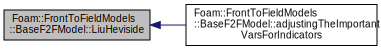
\includegraphics[width=350pt]{classFoam_1_1FrontToFieldModels_1_1BaseF2FModel_aa31e5f4538c17f43cb00f5885816b518_icgraph}
\end{center}
\end{figure}
\mbox{\Hypertarget{classFoam_1_1FrontToFieldModels_1_1BaseF2FModel_a1c6fcd79305e088eb8a66ce91307bc70}\label{classFoam_1_1FrontToFieldModels_1_1BaseF2FModel_a1c6fcd79305e088eb8a66ce91307bc70}} 
\index{Foam\+::\+Front\+To\+Field\+Models\+::\+Base\+F2\+F\+Model@{Foam\+::\+Front\+To\+Field\+Models\+::\+Base\+F2\+F\+Model}!m\+P\+QR@{m\+P\+QR}}
\index{m\+P\+QR@{m\+P\+QR}!Foam\+::\+Front\+To\+Field\+Models\+::\+Base\+F2\+F\+Model@{Foam\+::\+Front\+To\+Field\+Models\+::\+Base\+F2\+F\+Model}}
\subsubsection{\texorpdfstring{m\+P\+Q\+R()}{mPQR()}\hspace{0.1cm}{\footnotesize\ttfamily [1/2]}}
{\footnotesize\ttfamily template$<$class Cloud\+Type$>$ \\
scalar \hyperlink{classFoam_1_1FrontToFieldModels_1_1BaseF2FModel}{Foam\+::\+Front\+To\+Field\+Models\+::\+Base\+F2\+F\+Model}$<$ Cloud\+Type $>$\+::m\+P\+QR (\begin{DoxyParamCaption}\item[{vector}]{del,  }\item[{scalar}]{h,  }\item[{label}]{p,  }\item[{label}]{q,  }\item[{label}]{r }\end{DoxyParamCaption})\hspace{0.3cm}{\ttfamily [inline]}}

\mbox{\Hypertarget{classFoam_1_1FrontToFieldModels_1_1BaseF2FModel_abd3be11e7be0d82ed00f201a8b1ea48c}\label{classFoam_1_1FrontToFieldModels_1_1BaseF2FModel_abd3be11e7be0d82ed00f201a8b1ea48c}} 
\index{Foam\+::\+Front\+To\+Field\+Models\+::\+Base\+F2\+F\+Model@{Foam\+::\+Front\+To\+Field\+Models\+::\+Base\+F2\+F\+Model}!m\+P\+QR@{m\+P\+QR}}
\index{m\+P\+QR@{m\+P\+QR}!Foam\+::\+Front\+To\+Field\+Models\+::\+Base\+F2\+F\+Model@{Foam\+::\+Front\+To\+Field\+Models\+::\+Base\+F2\+F\+Model}}
\subsubsection{\texorpdfstring{m\+P\+Q\+R()}{mPQR()}\hspace{0.1cm}{\footnotesize\ttfamily [2/2]}}
{\footnotesize\ttfamily template$<$class Cloud\+Type $>$ \\
Foam\+::scalar \hyperlink{classFoam_1_1FrontToFieldModels_1_1BaseF2FModel}{Foam\+::\+Front\+To\+Field\+Models\+::\+Base\+F2\+F\+Model}$<$ Cloud\+Type $>$\+::m\+P\+QR (\begin{DoxyParamCaption}\item[{vector}]{del,  }\item[{scalar}]{h,  }\item[{label}]{p,  }\item[{label}]{q,  }\item[{label}]{r }\end{DoxyParamCaption})\hspace{0.3cm}{\ttfamily [inline]}}

\mbox{\Hypertarget{classFoam_1_1FrontToFieldModels_1_1BaseF2FModel_a1d1e01607afc846240ff156850e9da36}\label{classFoam_1_1FrontToFieldModels_1_1BaseF2FModel_a1d1e01607afc846240ff156850e9da36}} 
\index{Foam\+::\+Front\+To\+Field\+Models\+::\+Base\+F2\+F\+Model@{Foam\+::\+Front\+To\+Field\+Models\+::\+Base\+F2\+F\+Model}!PeskinD@{PeskinD}}
\index{PeskinD@{PeskinD}!Foam\+::\+Front\+To\+Field\+Models\+::\+Base\+F2\+F\+Model@{Foam\+::\+Front\+To\+Field\+Models\+::\+Base\+F2\+F\+Model}}
\subsubsection{\texorpdfstring{Peskin\+D()}{PeskinD()}\hspace{0.1cm}{\footnotesize\ttfamily [1/2]}}
{\footnotesize\ttfamily template$<$class Cloud\+Type $>$ \\
Foam\+::scalar \hyperlink{classFoam_1_1FrontToFieldModels_1_1BaseF2FModel}{Foam\+::\+Front\+To\+Field\+Models\+::\+Base\+F2\+F\+Model}$<$ Cloud\+Type $>$\+::PeskinD (\begin{DoxyParamCaption}\item[{scalar}]{r,  }\item[{scalar}]{h }\end{DoxyParamCaption})\hspace{0.3cm}{\ttfamily [inline]}}

\mbox{\Hypertarget{classFoam_1_1FrontToFieldModels_1_1BaseF2FModel_a8eaf0fc148f9a76dc85116567f12b3ce}\label{classFoam_1_1FrontToFieldModels_1_1BaseF2FModel_a8eaf0fc148f9a76dc85116567f12b3ce}} 
\index{Foam\+::\+Front\+To\+Field\+Models\+::\+Base\+F2\+F\+Model@{Foam\+::\+Front\+To\+Field\+Models\+::\+Base\+F2\+F\+Model}!PeskinD@{PeskinD}}
\index{PeskinD@{PeskinD}!Foam\+::\+Front\+To\+Field\+Models\+::\+Base\+F2\+F\+Model@{Foam\+::\+Front\+To\+Field\+Models\+::\+Base\+F2\+F\+Model}}
\subsubsection{\texorpdfstring{Peskin\+D()}{PeskinD()}\hspace{0.1cm}{\footnotesize\ttfamily [2/2]}}
{\footnotesize\ttfamily template$<$class Cloud\+Type$>$ \\
scalar \hyperlink{classFoam_1_1FrontToFieldModels_1_1BaseF2FModel}{Foam\+::\+Front\+To\+Field\+Models\+::\+Base\+F2\+F\+Model}$<$ Cloud\+Type $>$\+::PeskinD (\begin{DoxyParamCaption}\item[{scalar}]{r,  }\item[{scalar}]{h }\end{DoxyParamCaption})\hspace{0.3cm}{\ttfamily [inline]}}

\mbox{\Hypertarget{classFoam_1_1FrontToFieldModels_1_1BaseF2FModel_a25864f279b675ee9ba440f5d9b874b46}\label{classFoam_1_1FrontToFieldModels_1_1BaseF2FModel_a25864f279b675ee9ba440f5d9b874b46}} 
\index{Foam\+::\+Front\+To\+Field\+Models\+::\+Base\+F2\+F\+Model@{Foam\+::\+Front\+To\+Field\+Models\+::\+Base\+F2\+F\+Model}!window\+Func@{window\+Func}}
\index{window\+Func@{window\+Func}!Foam\+::\+Front\+To\+Field\+Models\+::\+Base\+F2\+F\+Model@{Foam\+::\+Front\+To\+Field\+Models\+::\+Base\+F2\+F\+Model}}
\subsubsection{\texorpdfstring{window\+Func()}{windowFunc()}\hspace{0.1cm}{\footnotesize\ttfamily [1/2]}}
{\footnotesize\ttfamily template$<$class Cloud\+Type$>$ \\
scalar \hyperlink{classFoam_1_1FrontToFieldModels_1_1BaseF2FModel}{Foam\+::\+Front\+To\+Field\+Models\+::\+Base\+F2\+F\+Model}$<$ Cloud\+Type $>$\+::window\+Func (\begin{DoxyParamCaption}\item[{vector}]{del,  }\item[{scalar}]{h }\end{DoxyParamCaption})\hspace{0.3cm}{\ttfamily [inline]}}

\mbox{\Hypertarget{classFoam_1_1FrontToFieldModels_1_1BaseF2FModel_a022f033f51b4ddb89082282d4e92ae9f}\label{classFoam_1_1FrontToFieldModels_1_1BaseF2FModel_a022f033f51b4ddb89082282d4e92ae9f}} 
\index{Foam\+::\+Front\+To\+Field\+Models\+::\+Base\+F2\+F\+Model@{Foam\+::\+Front\+To\+Field\+Models\+::\+Base\+F2\+F\+Model}!window\+Func@{window\+Func}}
\index{window\+Func@{window\+Func}!Foam\+::\+Front\+To\+Field\+Models\+::\+Base\+F2\+F\+Model@{Foam\+::\+Front\+To\+Field\+Models\+::\+Base\+F2\+F\+Model}}
\subsubsection{\texorpdfstring{window\+Func()}{windowFunc()}\hspace{0.1cm}{\footnotesize\ttfamily [2/2]}}
{\footnotesize\ttfamily template$<$class Cloud\+Type $>$ \\
Foam\+::scalar \hyperlink{classFoam_1_1FrontToFieldModels_1_1BaseF2FModel}{Foam\+::\+Front\+To\+Field\+Models\+::\+Base\+F2\+F\+Model}$<$ Cloud\+Type $>$\+::window\+Func (\begin{DoxyParamCaption}\item[{vector}]{del,  }\item[{scalar}]{h }\end{DoxyParamCaption})\hspace{0.3cm}{\ttfamily [inline]}}

\mbox{\Hypertarget{classFoam_1_1FrontToFieldModels_1_1BaseF2FModel_af004d7b781e7e2a176b1ece4aee02a81}\label{classFoam_1_1FrontToFieldModels_1_1BaseF2FModel_af004d7b781e7e2a176b1ece4aee02a81}} 
\index{Foam\+::\+Front\+To\+Field\+Models\+::\+Base\+F2\+F\+Model@{Foam\+::\+Front\+To\+Field\+Models\+::\+Base\+F2\+F\+Model}!window\+Func\+Bar@{window\+Func\+Bar}}
\index{window\+Func\+Bar@{window\+Func\+Bar}!Foam\+::\+Front\+To\+Field\+Models\+::\+Base\+F2\+F\+Model@{Foam\+::\+Front\+To\+Field\+Models\+::\+Base\+F2\+F\+Model}}
\subsubsection{\texorpdfstring{window\+Func\+Bar()}{windowFuncBar()}\hspace{0.1cm}{\footnotesize\ttfamily [1/2]}}
{\footnotesize\ttfamily template$<$class Cloud\+Type $>$ \\
Foam\+::scalar \hyperlink{classFoam_1_1FrontToFieldModels_1_1BaseF2FModel}{Foam\+::\+Front\+To\+Field\+Models\+::\+Base\+F2\+F\+Model}$<$ Cloud\+Type $>$\+::window\+Func\+Bar (\begin{DoxyParamCaption}\item[{vector}]{del,  }\item[{scalar}]{h,  }\item[{List$<$ scalar $>$}]{beta }\end{DoxyParamCaption})\hspace{0.3cm}{\ttfamily [inline]}}

\mbox{\Hypertarget{classFoam_1_1FrontToFieldModels_1_1BaseF2FModel_ab75791ed7cb3eb23ffa0cc29d464b7cc}\label{classFoam_1_1FrontToFieldModels_1_1BaseF2FModel_ab75791ed7cb3eb23ffa0cc29d464b7cc}} 
\index{Foam\+::\+Front\+To\+Field\+Models\+::\+Base\+F2\+F\+Model@{Foam\+::\+Front\+To\+Field\+Models\+::\+Base\+F2\+F\+Model}!window\+Func\+Bar@{window\+Func\+Bar}}
\index{window\+Func\+Bar@{window\+Func\+Bar}!Foam\+::\+Front\+To\+Field\+Models\+::\+Base\+F2\+F\+Model@{Foam\+::\+Front\+To\+Field\+Models\+::\+Base\+F2\+F\+Model}}
\subsubsection{\texorpdfstring{window\+Func\+Bar()}{windowFuncBar()}\hspace{0.1cm}{\footnotesize\ttfamily [2/2]}}
{\footnotesize\ttfamily template$<$class Cloud\+Type$>$ \\
scalar \hyperlink{classFoam_1_1FrontToFieldModels_1_1BaseF2FModel}{Foam\+::\+Front\+To\+Field\+Models\+::\+Base\+F2\+F\+Model}$<$ Cloud\+Type $>$\+::window\+Func\+Bar (\begin{DoxyParamCaption}\item[{vector}]{del,  }\item[{scalar}]{h,  }\item[{List$<$ scalar $>$}]{beta }\end{DoxyParamCaption})\hspace{0.3cm}{\ttfamily [inline]}}



\subsection{Member Data Documentation}
\mbox{\Hypertarget{classFoam_1_1FrontToFieldModels_1_1BaseF2FModel_a28af8ea6a018505dfd6618cbfe8d4a31}\label{classFoam_1_1FrontToFieldModels_1_1BaseF2FModel_a28af8ea6a018505dfd6618cbfe8d4a31}} 
\index{Foam\+::\+Front\+To\+Field\+Models\+::\+Base\+F2\+F\+Model@{Foam\+::\+Front\+To\+Field\+Models\+::\+Base\+F2\+F\+Model}!beta\+\_\+@{beta\+\_\+}}
\index{beta\+\_\+@{beta\+\_\+}!Foam\+::\+Front\+To\+Field\+Models\+::\+Base\+F2\+F\+Model@{Foam\+::\+Front\+To\+Field\+Models\+::\+Base\+F2\+F\+Model}}
\subsubsection{\texorpdfstring{beta\+\_\+}{beta\_}}
{\footnotesize\ttfamily template$<$class Cloud\+Type$>$ \\
List$<$ scalar $>$ \hyperlink{classFoam_1_1FrontToFieldModels_1_1BaseF2FModel}{Foam\+::\+Front\+To\+Field\+Models\+::\+Base\+F2\+F\+Model}$<$ Cloud\+Type $>$\+::beta\+\_\+}

\mbox{\Hypertarget{classFoam_1_1FrontToFieldModels_1_1BaseF2FModel_a1bcf6f9b3c688869536482e9ac76eda3}\label{classFoam_1_1FrontToFieldModels_1_1BaseF2FModel_a1bcf6f9b3c688869536482e9ac76eda3}} 
\index{Foam\+::\+Front\+To\+Field\+Models\+::\+Base\+F2\+F\+Model@{Foam\+::\+Front\+To\+Field\+Models\+::\+Base\+F2\+F\+Model}!filtering\+Weight\+\_\+@{filtering\+Weight\+\_\+}}
\index{filtering\+Weight\+\_\+@{filtering\+Weight\+\_\+}!Foam\+::\+Front\+To\+Field\+Models\+::\+Base\+F2\+F\+Model@{Foam\+::\+Front\+To\+Field\+Models\+::\+Base\+F2\+F\+Model}}
\subsubsection{\texorpdfstring{filtering\+Weight\+\_\+}{filteringWeight\_}}
{\footnotesize\ttfamily template$<$class Cloud\+Type$>$ \\
scalar \hyperlink{classFoam_1_1FrontToFieldModels_1_1BaseF2FModel}{Foam\+::\+Front\+To\+Field\+Models\+::\+Base\+F2\+F\+Model}$<$ Cloud\+Type $>$\+::filtering\+Weight\+\_\+ = 0.\+0}

\mbox{\Hypertarget{classFoam_1_1FrontToFieldModels_1_1BaseF2FModel_a0e777bd8fd5a92cc3e9a8833a53be8a3}\label{classFoam_1_1FrontToFieldModels_1_1BaseF2FModel_a0e777bd8fd5a92cc3e9a8833a53be8a3}} 
\index{Foam\+::\+Front\+To\+Field\+Models\+::\+Base\+F2\+F\+Model@{Foam\+::\+Front\+To\+Field\+Models\+::\+Base\+F2\+F\+Model}!front2field\+\_\+@{front2field\+\_\+}}
\index{front2field\+\_\+@{front2field\+\_\+}!Foam\+::\+Front\+To\+Field\+Models\+::\+Base\+F2\+F\+Model@{Foam\+::\+Front\+To\+Field\+Models\+::\+Base\+F2\+F\+Model}}
\subsubsection{\texorpdfstring{front2field\+\_\+}{front2field\_}}
{\footnotesize\ttfamily template$<$class Cloud\+Type$>$ \\
word \hyperlink{classFoam_1_1FrontToFieldModels_1_1BaseF2FModel}{Foam\+::\+Front\+To\+Field\+Models\+::\+Base\+F2\+F\+Model}$<$ Cloud\+Type $>$\+::front2field\+\_\+}

\mbox{\Hypertarget{classFoam_1_1FrontToFieldModels_1_1BaseF2FModel_a72b788105fc00ea41d1b1be73e18e6a2}\label{classFoam_1_1FrontToFieldModels_1_1BaseF2FModel_a72b788105fc00ea41d1b1be73e18e6a2}} 
\index{Foam\+::\+Front\+To\+Field\+Models\+::\+Base\+F2\+F\+Model@{Foam\+::\+Front\+To\+Field\+Models\+::\+Base\+F2\+F\+Model}!number\+Of\+Indicator\+Filtering\+\_\+@{number\+Of\+Indicator\+Filtering\+\_\+}}
\index{number\+Of\+Indicator\+Filtering\+\_\+@{number\+Of\+Indicator\+Filtering\+\_\+}!Foam\+::\+Front\+To\+Field\+Models\+::\+Base\+F2\+F\+Model@{Foam\+::\+Front\+To\+Field\+Models\+::\+Base\+F2\+F\+Model}}
\subsubsection{\texorpdfstring{number\+Of\+Indicator\+Filtering\+\_\+}{numberOfIndicatorFiltering\_}}
{\footnotesize\ttfamily template$<$class Cloud\+Type$>$ \\
label \hyperlink{classFoam_1_1FrontToFieldModels_1_1BaseF2FModel}{Foam\+::\+Front\+To\+Field\+Models\+::\+Base\+F2\+F\+Model}$<$ Cloud\+Type $>$\+::number\+Of\+Indicator\+Filtering\+\_\+ = 0}

\mbox{\Hypertarget{classFoam_1_1FrontToFieldModels_1_1BaseF2FModel_a55b6ed327c5b3b4360d4a4f537a5e41e}\label{classFoam_1_1FrontToFieldModels_1_1BaseF2FModel_a55b6ed327c5b3b4360d4a4f537a5e41e}} 
\index{Foam\+::\+Front\+To\+Field\+Models\+::\+Base\+F2\+F\+Model@{Foam\+::\+Front\+To\+Field\+Models\+::\+Base\+F2\+F\+Model}!p\+\_\+@{p\+\_\+}}
\index{p\+\_\+@{p\+\_\+}!Foam\+::\+Front\+To\+Field\+Models\+::\+Base\+F2\+F\+Model@{Foam\+::\+Front\+To\+Field\+Models\+::\+Base\+F2\+F\+Model}}
\subsubsection{\texorpdfstring{p\+\_\+}{p\_}}
{\footnotesize\ttfamily template$<$class Cloud\+Type$>$ \\
List$<$ label $>$ \hyperlink{classFoam_1_1FrontToFieldModels_1_1BaseF2FModel}{Foam\+::\+Front\+To\+Field\+Models\+::\+Base\+F2\+F\+Model}$<$ Cloud\+Type $>$\+::p\+\_\+}

\mbox{\Hypertarget{classFoam_1_1FrontToFieldModels_1_1BaseF2FModel_ae2f7cdcbcd60d5a849afc352765cdefe}\label{classFoam_1_1FrontToFieldModels_1_1BaseF2FModel_ae2f7cdcbcd60d5a849afc352765cdefe}} 
\index{Foam\+::\+Front\+To\+Field\+Models\+::\+Base\+F2\+F\+Model@{Foam\+::\+Front\+To\+Field\+Models\+::\+Base\+F2\+F\+Model}!q\+\_\+@{q\+\_\+}}
\index{q\+\_\+@{q\+\_\+}!Foam\+::\+Front\+To\+Field\+Models\+::\+Base\+F2\+F\+Model@{Foam\+::\+Front\+To\+Field\+Models\+::\+Base\+F2\+F\+Model}}
\subsubsection{\texorpdfstring{q\+\_\+}{q\_}}
{\footnotesize\ttfamily template$<$class Cloud\+Type$>$ \\
List$<$ label $>$ \hyperlink{classFoam_1_1FrontToFieldModels_1_1BaseF2FModel}{Foam\+::\+Front\+To\+Field\+Models\+::\+Base\+F2\+F\+Model}$<$ Cloud\+Type $>$\+::q\+\_\+}

\mbox{\Hypertarget{classFoam_1_1FrontToFieldModels_1_1BaseF2FModel_a2f335eed9c03847c9a84ad4d8d3bfa98}\label{classFoam_1_1FrontToFieldModels_1_1BaseF2FModel_a2f335eed9c03847c9a84ad4d8d3bfa98}} 
\index{Foam\+::\+Front\+To\+Field\+Models\+::\+Base\+F2\+F\+Model@{Foam\+::\+Front\+To\+Field\+Models\+::\+Base\+F2\+F\+Model}!r\+\_\+@{r\+\_\+}}
\index{r\+\_\+@{r\+\_\+}!Foam\+::\+Front\+To\+Field\+Models\+::\+Base\+F2\+F\+Model@{Foam\+::\+Front\+To\+Field\+Models\+::\+Base\+F2\+F\+Model}}
\subsubsection{\texorpdfstring{r\+\_\+}{r\_}}
{\footnotesize\ttfamily template$<$class Cloud\+Type$>$ \\
List$<$ label $>$ \hyperlink{classFoam_1_1FrontToFieldModels_1_1BaseF2FModel}{Foam\+::\+Front\+To\+Field\+Models\+::\+Base\+F2\+F\+Model}$<$ Cloud\+Type $>$\+::r\+\_\+}

\mbox{\Hypertarget{classFoam_1_1FrontToFieldModels_1_1BaseF2FModel_ac944d075a159992d2e38d2d9c0eb5c2e}\label{classFoam_1_1FrontToFieldModels_1_1BaseF2FModel_ac944d075a159992d2e38d2d9c0eb5c2e}} 
\index{Foam\+::\+Front\+To\+Field\+Models\+::\+Base\+F2\+F\+Model@{Foam\+::\+Front\+To\+Field\+Models\+::\+Base\+F2\+F\+Model}!spreading\+Option\+\_\+@{spreading\+Option\+\_\+}}
\index{spreading\+Option\+\_\+@{spreading\+Option\+\_\+}!Foam\+::\+Front\+To\+Field\+Models\+::\+Base\+F2\+F\+Model@{Foam\+::\+Front\+To\+Field\+Models\+::\+Base\+F2\+F\+Model}}
\subsubsection{\texorpdfstring{spreading\+Option\+\_\+}{spreadingOption\_}}
{\footnotesize\ttfamily template$<$class Cloud\+Type$>$ \\
\hyperlink{classFoam_1_1FrontToFieldModels_1_1BaseF2FModel_a16ac12059f9cdbf69d5bef5029e9e2f3}{spreading\+Option} \hyperlink{classFoam_1_1FrontToFieldModels_1_1BaseF2FModel}{Foam\+::\+Front\+To\+Field\+Models\+::\+Base\+F2\+F\+Model}$<$ Cloud\+Type $>$\+::spreading\+Option\+\_\+}



The documentation for this class was generated from the following files\+:\begin{DoxyCompactItemize}
\item 
ln\+Include/\hyperlink{lnInclude_2BaseF2FModel_8H}{Base\+F2\+F\+Model.\+H}\item 
ln\+Include/\hyperlink{lnInclude_2BaseF2FModel_8C}{Base\+F2\+F\+Model.\+C}\end{DoxyCompactItemize}

\hypertarget{classFoam_1_1bubbleData}{}\section{Foam\+:\+:bubble\+Data Class Reference}
\label{classFoam_1_1bubbleData}\index{Foam\+::bubble\+Data@{Foam\+::bubble\+Data}}


{\ttfamily \#include $<$bubble\+Data.\+H$>$}



Collaboration diagram for Foam\+:\+:bubble\+Data\+:\nopagebreak
\begin{figure}[H]
\begin{center}
\leavevmode
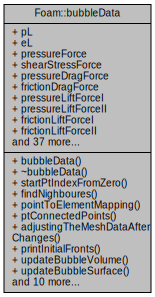
\includegraphics[width=227pt]{classFoam_1_1bubbleData__coll__graph}
\end{center}
\end{figure}
\subsection*{Public Member Functions}
\begin{DoxyCompactItemize}
\item 
\hyperlink{classFoam_1_1bubbleData_a78c0f6a3fff15dd2239fefd25ffbe0ff}{bubble\+Data} ()
\item 
virtual \hyperlink{classFoam_1_1bubbleData_adede9b130e190142e610d9b5f8cbdb7e}{$\sim$bubble\+Data} ()
\item 
void \hyperlink{classFoam_1_1bubbleData_a01a4a0bd51dfdfd148cd09f173c42443}{start\+Pt\+Index\+From\+Zero} ()
\item 
void \hyperlink{classFoam_1_1bubbleData_a200b32da9651717744e2c042c708550a}{find\+Nighboures} ()
\item 
void \hyperlink{classFoam_1_1bubbleData_acda4c6cfdf009e8e11f7b8f2d6b161dc}{point\+To\+Element\+Mapping} ()
\item 
void \hyperlink{classFoam_1_1bubbleData_ae39fb04d51d3f94e71b2f5c39e5b6c56}{pt\+Connected\+Points} ()
\item 
label\+List \hyperlink{classFoam_1_1bubbleData_a8b33b963edbce17b6595f75259622ada}{adjusting\+The\+Mesh\+Data\+After\+Changes} ()
\item 
void \hyperlink{classFoam_1_1bubbleData_a7bc4465328f4b231c17305a76db1d8a1}{print\+Initial\+Fronts} (const file\+Name \&outfile\+Name)
\item 
void \hyperlink{classFoam_1_1bubbleData_aa62a18b88be0327ed56c49a48cc2820b}{update\+Bubble\+Volume} ()
\item 
void \hyperlink{classFoam_1_1bubbleData_aeca8b64dfc956cf92b07fc98de0b1fb3}{update\+Bubble\+Surface} ()
\item 
\hyperlink{classFoam_1_1bubbleData_a78c0f6a3fff15dd2239fefd25ffbe0ff}{bubble\+Data} ()
\item 
virtual \hyperlink{classFoam_1_1bubbleData_adede9b130e190142e610d9b5f8cbdb7e}{$\sim$bubble\+Data} ()
\item 
void \hyperlink{classFoam_1_1bubbleData_a01a4a0bd51dfdfd148cd09f173c42443}{start\+Pt\+Index\+From\+Zero} ()
\item 
void \hyperlink{classFoam_1_1bubbleData_a200b32da9651717744e2c042c708550a}{find\+Nighboures} ()
\item 
void \hyperlink{classFoam_1_1bubbleData_acda4c6cfdf009e8e11f7b8f2d6b161dc}{point\+To\+Element\+Mapping} ()
\item 
void \hyperlink{classFoam_1_1bubbleData_ae39fb04d51d3f94e71b2f5c39e5b6c56}{pt\+Connected\+Points} ()
\item 
label\+List \hyperlink{classFoam_1_1bubbleData_a54f47b20e06cb8572df1ae28e5bf5902}{adjusting\+The\+Mesh\+Data\+After\+Changes} ()
\item 
void \hyperlink{classFoam_1_1bubbleData_a7bc4465328f4b231c17305a76db1d8a1}{print\+Initial\+Fronts} (const file\+Name \&outfile\+Name)
\item 
void \hyperlink{classFoam_1_1bubbleData_aa62a18b88be0327ed56c49a48cc2820b}{update\+Bubble\+Volume} ()
\item 
void \hyperlink{classFoam_1_1bubbleData_aeca8b64dfc956cf92b07fc98de0b1fb3}{update\+Bubble\+Surface} ()
\end{DoxyCompactItemize}
\subsection*{Public Attributes}
\begin{DoxyCompactItemize}
\item 
Dynamic\+List$<$ \hyperlink{classFoam_1_1pointData}{point\+Data} $>$ \hyperlink{classFoam_1_1bubbleData_a466b40438d465e522c6cf9b6ae042638}{pL}
\item 
Dynamic\+List$<$ \hyperlink{classFoam_1_1elementInfo}{element\+Info} $>$ \hyperlink{classFoam_1_1bubbleData_a8b56f8139f82c448103b2f8296be3587}{eL}
\item 
vector \hyperlink{classFoam_1_1bubbleData_a0a3b90c342d0c81cce02aa50fe650b4f}{pressure\+Force}
\item 
vector \hyperlink{classFoam_1_1bubbleData_af3b01e31394ca2db56831b637c823fad}{shear\+Stress\+Force}
\item 
scalar \hyperlink{classFoam_1_1bubbleData_abf4def2ca2031f32ef6d3d9039fe659b}{pressure\+Drag\+Force}
\item 
scalar \hyperlink{classFoam_1_1bubbleData_ab0498b3d44aa2e83e63c60de8a2dcefa}{friction\+Drag\+Force}
\item 
scalar \hyperlink{classFoam_1_1bubbleData_a3c93a65a6c6d39068229947c01c7d06d}{pressure\+Lift\+ForceI}
\item 
scalar \hyperlink{classFoam_1_1bubbleData_a9ab24dd7989a030ca7c038336bdfcec9}{pressure\+Lift\+Force\+II}
\item 
scalar \hyperlink{classFoam_1_1bubbleData_aba3c36d8dee4a54fd00e7f03c0e99b3e}{friction\+Lift\+ForceI}
\item 
scalar \hyperlink{classFoam_1_1bubbleData_a611eb9b38cad5263f53ae226ab5af33b}{friction\+Lift\+Force\+II}
\item 
scalar \hyperlink{classFoam_1_1bubbleData_a37593f268513154da15399f5d346161a}{total\+Drag\+Force}
\item 
scalar \hyperlink{classFoam_1_1bubbleData_a46b4565cc9a62aa11f8ababc548115d8}{total\+Lift\+ForceI}
\item 
scalar \hyperlink{classFoam_1_1bubbleData_af405b224178a16813fed947591cb1bff}{total\+Lift\+Force\+II}
\item 
vector \hyperlink{classFoam_1_1bubbleData_a26444575af04c6f0b29a04fcc323e7b5}{buoyant\+Force}
\item 
vector \hyperlink{classFoam_1_1bubbleData_a377d050bf5cccc31cb1842a7471f0b40}{gravity\+Force}
\item 
vector \hyperlink{classFoam_1_1bubbleData_acd5cb743fe1daca143e57e30f6ef6487}{accelaration}
\item 
vector \hyperlink{classFoam_1_1bubbleData_a6f24e8e0d7d406bc0fce92c61c7b9f6a}{velocity}
\item 
vector \hyperlink{classFoam_1_1bubbleData_a2ddfba5a0c373cf04288b484a3f20b1e}{velocity\+Old}
\item 
vector \hyperlink{classFoam_1_1bubbleData_a71a1e15224b7eac3f2411eba31f9b245}{centre}
\item 
vector \hyperlink{classFoam_1_1bubbleData_a07eabe2600aba9ae1b8f8722baa2e929}{centre\+Old}
\item 
scalar \hyperlink{classFoam_1_1bubbleData_af26ac17dd3c8484703b484b1a0b406f6}{volume}
\item 
scalar \hyperlink{classFoam_1_1bubbleData_a8542e54692c07cedc2c0cae2a74ba24d}{volume0}
\item 
scalar \hyperlink{classFoam_1_1bubbleData_afa34821682366185de9b87a483dd6f43}{surface\+Area}
\item 
scalar \hyperlink{classFoam_1_1bubbleData_a956a6ca9a5125d1b0ccb94bd2487ca29}{mass}
\item 
scalar \hyperlink{classFoam_1_1bubbleData_a35633f81703ca31b7b06cdbc51218991}{density}
\item 
scalar \hyperlink{classFoam_1_1bubbleData_a181098e2c93266f0b4c6861522b478b3}{outer\+Fluid\+Density}
\item 
scalar \hyperlink{classFoam_1_1bubbleData_a82b5b5338bb0d363e79e8078d84fbdaf}{viscosity}
\item 
scalar \hyperlink{classFoam_1_1bubbleData_a20908303d8e37f882e52595d1da9beb1}{outer\+Fluid\+Viscosity}
\item 
scalar \hyperlink{classFoam_1_1bubbleData_add40c043c47fac7ac16bff1e03823dca}{drag\+Coeff}
\item 
scalar \hyperlink{classFoam_1_1bubbleData_ada8e7f1dc0b9a282f63a8a777a70cef5}{Lift\+CoeffI}
\item 
scalar \hyperlink{classFoam_1_1bubbleData_a7bad7043d9e915dd6aabc47608b114e5}{Lift\+Coeff\+II}
\item 
label \hyperlink{classFoam_1_1bubbleData_afab8b5aa167b02470788d3f3d4b3d7cd}{current\+Index}
\item 
scalar \hyperlink{classFoam_1_1bubbleData_aec394160aa23b63eb672846179287f8e}{surface\+Tension\+Coeff}
\item 
scalar \hyperlink{classFoam_1_1bubbleData_af3720d63ef807c83c099b3ad7dd77f5d}{Morton\+Number}
\item 
scalar \hyperlink{classFoam_1_1bubbleData_a6256640184e8fe3c9e55aade352ea782}{Eotvos\+Number}
\item 
scalar \hyperlink{classFoam_1_1bubbleData_a0427ab63bc536b2b2ac8b0e372828f5e}{sphere\+Bubble\+Diameter}
\item 
List$<$ scalar $>$ \hyperlink{classFoam_1_1bubbleData_a2bf3e3d90a32e574d289d88ff5b2f2ed}{diameter}
\item 
scalar \hyperlink{classFoam_1_1bubbleData_a7ba3dffa9c8bf20077966d44c2a3fd9d}{sphericity}
\item 
vector \hyperlink{classFoam_1_1bubbleData_a9f920dfaf0d1f9da22207d08b8e1cbc1}{pressure\+Jump\+At\+The\+Interface}
\item 
bool \hyperlink{classFoam_1_1bubbleData_aa40fd779e46229fc8c402c46d75fad8d}{keep\+Bubble}
\item 
bool \hyperlink{classFoam_1_1bubbleData_a9d67f3633db9de211d0a8bf4d6a70fd8}{el\+Neighbor\+Flag}
\item 
bool \hyperlink{classFoam_1_1bubbleData_aefeccb5501bc3d113b6fef02a3ea2bae}{el\+Points\+Flag}
\item 
bool \hyperlink{classFoam_1_1bubbleData_a15e8c5d0bd3a677e2d81c2b4ebe50dea}{pl\+Connection\+Flag}
\item 
bool \hyperlink{classFoam_1_1bubbleData_acf7c9565ddd9cc8235769a19707b3451}{el\+Surface\+Flag}
\item 
bool \hyperlink{classFoam_1_1bubbleData_ae83882aee8f42d1d3e3fd1c42610beb6}{volume\+Flag}
\item 
bool \hyperlink{classFoam_1_1bubbleData_aa9c8dd1bfe64b2f19dc441d87b888d9c}{p\+L\+Pos\+In\+Domain\+Flag}
\item 
bool \hyperlink{classFoam_1_1bubbleData_ae0a6387d9d99d4d6ce94e0ccb265f5d2}{el\+C\+Pos\+In\+Domain\+Flag}
\end{DoxyCompactItemize}


\subsection{Constructor \& Destructor Documentation}
\mbox{\Hypertarget{classFoam_1_1bubbleData_a78c0f6a3fff15dd2239fefd25ffbe0ff}\label{classFoam_1_1bubbleData_a78c0f6a3fff15dd2239fefd25ffbe0ff}} 
\index{Foam\+::bubble\+Data@{Foam\+::bubble\+Data}!bubble\+Data@{bubble\+Data}}
\index{bubble\+Data@{bubble\+Data}!Foam\+::bubble\+Data@{Foam\+::bubble\+Data}}
\subsubsection{\texorpdfstring{bubble\+Data()}{bubbleData()}\hspace{0.1cm}{\footnotesize\ttfamily [1/2]}}
{\footnotesize\ttfamily Foam\+::bubble\+Data\+::bubble\+Data (\begin{DoxyParamCaption}{ }\end{DoxyParamCaption})\hspace{0.3cm}{\ttfamily [inline]}}

\mbox{\Hypertarget{classFoam_1_1bubbleData_adede9b130e190142e610d9b5f8cbdb7e}\label{classFoam_1_1bubbleData_adede9b130e190142e610d9b5f8cbdb7e}} 
\index{Foam\+::bubble\+Data@{Foam\+::bubble\+Data}!````~bubble\+Data@{$\sim$bubble\+Data}}
\index{````~bubble\+Data@{$\sim$bubble\+Data}!Foam\+::bubble\+Data@{Foam\+::bubble\+Data}}
\subsubsection{\texorpdfstring{$\sim$bubble\+Data()}{~bubbleData()}\hspace{0.1cm}{\footnotesize\ttfamily [1/2]}}
{\footnotesize\ttfamily virtual Foam\+::bubble\+Data\+::$\sim$bubble\+Data (\begin{DoxyParamCaption}{ }\end{DoxyParamCaption})\hspace{0.3cm}{\ttfamily [inline]}, {\ttfamily [virtual]}}

\mbox{\Hypertarget{classFoam_1_1bubbleData_a78c0f6a3fff15dd2239fefd25ffbe0ff}\label{classFoam_1_1bubbleData_a78c0f6a3fff15dd2239fefd25ffbe0ff}} 
\index{Foam\+::bubble\+Data@{Foam\+::bubble\+Data}!bubble\+Data@{bubble\+Data}}
\index{bubble\+Data@{bubble\+Data}!Foam\+::bubble\+Data@{Foam\+::bubble\+Data}}
\subsubsection{\texorpdfstring{bubble\+Data()}{bubbleData()}\hspace{0.1cm}{\footnotesize\ttfamily [2/2]}}
{\footnotesize\ttfamily Foam\+::bubble\+Data\+::bubble\+Data (\begin{DoxyParamCaption}{ }\end{DoxyParamCaption})\hspace{0.3cm}{\ttfamily [inline]}}

\mbox{\Hypertarget{classFoam_1_1bubbleData_adede9b130e190142e610d9b5f8cbdb7e}\label{classFoam_1_1bubbleData_adede9b130e190142e610d9b5f8cbdb7e}} 
\index{Foam\+::bubble\+Data@{Foam\+::bubble\+Data}!````~bubble\+Data@{$\sim$bubble\+Data}}
\index{````~bubble\+Data@{$\sim$bubble\+Data}!Foam\+::bubble\+Data@{Foam\+::bubble\+Data}}
\subsubsection{\texorpdfstring{$\sim$bubble\+Data()}{~bubbleData()}\hspace{0.1cm}{\footnotesize\ttfamily [2/2]}}
{\footnotesize\ttfamily virtual Foam\+::bubble\+Data\+::$\sim$bubble\+Data (\begin{DoxyParamCaption}{ }\end{DoxyParamCaption})\hspace{0.3cm}{\ttfamily [inline]}, {\ttfamily [virtual]}}



\subsection{Member Function Documentation}
\mbox{\Hypertarget{classFoam_1_1bubbleData_a8b33b963edbce17b6595f75259622ada}\label{classFoam_1_1bubbleData_a8b33b963edbce17b6595f75259622ada}} 
\index{Foam\+::bubble\+Data@{Foam\+::bubble\+Data}!adjusting\+The\+Mesh\+Data\+After\+Changes@{adjusting\+The\+Mesh\+Data\+After\+Changes}}
\index{adjusting\+The\+Mesh\+Data\+After\+Changes@{adjusting\+The\+Mesh\+Data\+After\+Changes}!Foam\+::bubble\+Data@{Foam\+::bubble\+Data}}
\subsubsection{\texorpdfstring{adjusting\+The\+Mesh\+Data\+After\+Changes()}{adjustingTheMeshDataAfterChanges()}\hspace{0.1cm}{\footnotesize\ttfamily [1/2]}}
{\footnotesize\ttfamily Foam\+::label\+List Foam\+::bubble\+Data\+::adjusting\+The\+Mesh\+Data\+After\+Changes (\begin{DoxyParamCaption}{ }\end{DoxyParamCaption})}

\mbox{\Hypertarget{classFoam_1_1bubbleData_a54f47b20e06cb8572df1ae28e5bf5902}\label{classFoam_1_1bubbleData_a54f47b20e06cb8572df1ae28e5bf5902}} 
\index{Foam\+::bubble\+Data@{Foam\+::bubble\+Data}!adjusting\+The\+Mesh\+Data\+After\+Changes@{adjusting\+The\+Mesh\+Data\+After\+Changes}}
\index{adjusting\+The\+Mesh\+Data\+After\+Changes@{adjusting\+The\+Mesh\+Data\+After\+Changes}!Foam\+::bubble\+Data@{Foam\+::bubble\+Data}}
\subsubsection{\texorpdfstring{adjusting\+The\+Mesh\+Data\+After\+Changes()}{adjustingTheMeshDataAfterChanges()}\hspace{0.1cm}{\footnotesize\ttfamily [2/2]}}
{\footnotesize\ttfamily label\+List Foam\+::bubble\+Data\+::adjusting\+The\+Mesh\+Data\+After\+Changes (\begin{DoxyParamCaption}{ }\end{DoxyParamCaption})}

\mbox{\Hypertarget{classFoam_1_1bubbleData_a200b32da9651717744e2c042c708550a}\label{classFoam_1_1bubbleData_a200b32da9651717744e2c042c708550a}} 
\index{Foam\+::bubble\+Data@{Foam\+::bubble\+Data}!find\+Nighboures@{find\+Nighboures}}
\index{find\+Nighboures@{find\+Nighboures}!Foam\+::bubble\+Data@{Foam\+::bubble\+Data}}
\subsubsection{\texorpdfstring{find\+Nighboures()}{findNighboures()}\hspace{0.1cm}{\footnotesize\ttfamily [1/2]}}
{\footnotesize\ttfamily void Foam\+::bubble\+Data\+::find\+Nighboures (\begin{DoxyParamCaption}{ }\end{DoxyParamCaption})}

Here is the caller graph for this function\+:\nopagebreak
\begin{figure}[H]
\begin{center}
\leavevmode
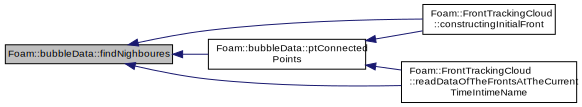
\includegraphics[width=350pt]{classFoam_1_1bubbleData_a200b32da9651717744e2c042c708550a_icgraph}
\end{center}
\end{figure}
\mbox{\Hypertarget{classFoam_1_1bubbleData_a200b32da9651717744e2c042c708550a}\label{classFoam_1_1bubbleData_a200b32da9651717744e2c042c708550a}} 
\index{Foam\+::bubble\+Data@{Foam\+::bubble\+Data}!find\+Nighboures@{find\+Nighboures}}
\index{find\+Nighboures@{find\+Nighboures}!Foam\+::bubble\+Data@{Foam\+::bubble\+Data}}
\subsubsection{\texorpdfstring{find\+Nighboures()}{findNighboures()}\hspace{0.1cm}{\footnotesize\ttfamily [2/2]}}
{\footnotesize\ttfamily void Foam\+::bubble\+Data\+::find\+Nighboures (\begin{DoxyParamCaption}{ }\end{DoxyParamCaption})}

\mbox{\Hypertarget{classFoam_1_1bubbleData_acda4c6cfdf009e8e11f7b8f2d6b161dc}\label{classFoam_1_1bubbleData_acda4c6cfdf009e8e11f7b8f2d6b161dc}} 
\index{Foam\+::bubble\+Data@{Foam\+::bubble\+Data}!point\+To\+Element\+Mapping@{point\+To\+Element\+Mapping}}
\index{point\+To\+Element\+Mapping@{point\+To\+Element\+Mapping}!Foam\+::bubble\+Data@{Foam\+::bubble\+Data}}
\subsubsection{\texorpdfstring{point\+To\+Element\+Mapping()}{pointToElementMapping()}\hspace{0.1cm}{\footnotesize\ttfamily [1/2]}}
{\footnotesize\ttfamily void Foam\+::bubble\+Data\+::point\+To\+Element\+Mapping (\begin{DoxyParamCaption}{ }\end{DoxyParamCaption})}

\mbox{\Hypertarget{classFoam_1_1bubbleData_acda4c6cfdf009e8e11f7b8f2d6b161dc}\label{classFoam_1_1bubbleData_acda4c6cfdf009e8e11f7b8f2d6b161dc}} 
\index{Foam\+::bubble\+Data@{Foam\+::bubble\+Data}!point\+To\+Element\+Mapping@{point\+To\+Element\+Mapping}}
\index{point\+To\+Element\+Mapping@{point\+To\+Element\+Mapping}!Foam\+::bubble\+Data@{Foam\+::bubble\+Data}}
\subsubsection{\texorpdfstring{point\+To\+Element\+Mapping()}{pointToElementMapping()}\hspace{0.1cm}{\footnotesize\ttfamily [2/2]}}
{\footnotesize\ttfamily void Foam\+::bubble\+Data\+::point\+To\+Element\+Mapping (\begin{DoxyParamCaption}{ }\end{DoxyParamCaption})}

Here is the caller graph for this function\+:\nopagebreak
\begin{figure}[H]
\begin{center}
\leavevmode
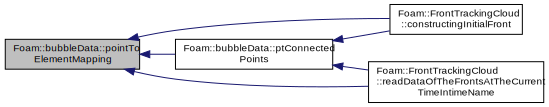
\includegraphics[width=350pt]{classFoam_1_1bubbleData_acda4c6cfdf009e8e11f7b8f2d6b161dc_icgraph}
\end{center}
\end{figure}
\mbox{\Hypertarget{classFoam_1_1bubbleData_a7bc4465328f4b231c17305a76db1d8a1}\label{classFoam_1_1bubbleData_a7bc4465328f4b231c17305a76db1d8a1}} 
\index{Foam\+::bubble\+Data@{Foam\+::bubble\+Data}!print\+Initial\+Fronts@{print\+Initial\+Fronts}}
\index{print\+Initial\+Fronts@{print\+Initial\+Fronts}!Foam\+::bubble\+Data@{Foam\+::bubble\+Data}}
\subsubsection{\texorpdfstring{print\+Initial\+Fronts()}{printInitialFronts()}\hspace{0.1cm}{\footnotesize\ttfamily [1/2]}}
{\footnotesize\ttfamily void Foam\+::bubble\+Data\+::print\+Initial\+Fronts (\begin{DoxyParamCaption}\item[{const file\+Name \&}]{outfile\+Name }\end{DoxyParamCaption})}

Here is the caller graph for this function\+:\nopagebreak
\begin{figure}[H]
\begin{center}
\leavevmode
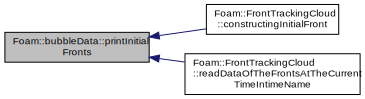
\includegraphics[width=350pt]{classFoam_1_1bubbleData_a7bc4465328f4b231c17305a76db1d8a1_icgraph}
\end{center}
\end{figure}
\mbox{\Hypertarget{classFoam_1_1bubbleData_a7bc4465328f4b231c17305a76db1d8a1}\label{classFoam_1_1bubbleData_a7bc4465328f4b231c17305a76db1d8a1}} 
\index{Foam\+::bubble\+Data@{Foam\+::bubble\+Data}!print\+Initial\+Fronts@{print\+Initial\+Fronts}}
\index{print\+Initial\+Fronts@{print\+Initial\+Fronts}!Foam\+::bubble\+Data@{Foam\+::bubble\+Data}}
\subsubsection{\texorpdfstring{print\+Initial\+Fronts()}{printInitialFronts()}\hspace{0.1cm}{\footnotesize\ttfamily [2/2]}}
{\footnotesize\ttfamily void Foam\+::bubble\+Data\+::print\+Initial\+Fronts (\begin{DoxyParamCaption}\item[{const file\+Name \&}]{outfile\+Name }\end{DoxyParamCaption})}

\mbox{\Hypertarget{classFoam_1_1bubbleData_ae39fb04d51d3f94e71b2f5c39e5b6c56}\label{classFoam_1_1bubbleData_ae39fb04d51d3f94e71b2f5c39e5b6c56}} 
\index{Foam\+::bubble\+Data@{Foam\+::bubble\+Data}!pt\+Connected\+Points@{pt\+Connected\+Points}}
\index{pt\+Connected\+Points@{pt\+Connected\+Points}!Foam\+::bubble\+Data@{Foam\+::bubble\+Data}}
\subsubsection{\texorpdfstring{pt\+Connected\+Points()}{ptConnectedPoints()}\hspace{0.1cm}{\footnotesize\ttfamily [1/2]}}
{\footnotesize\ttfamily void Foam\+::bubble\+Data\+::pt\+Connected\+Points (\begin{DoxyParamCaption}{ }\end{DoxyParamCaption})}

Here is the call graph for this function\+:\nopagebreak
\begin{figure}[H]
\begin{center}
\leavevmode
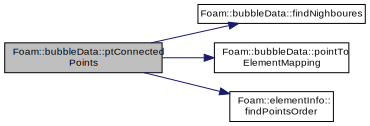
\includegraphics[width=350pt]{classFoam_1_1bubbleData_ae39fb04d51d3f94e71b2f5c39e5b6c56_cgraph}
\end{center}
\end{figure}
Here is the caller graph for this function\+:\nopagebreak
\begin{figure}[H]
\begin{center}
\leavevmode
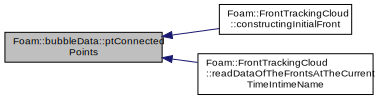
\includegraphics[width=350pt]{classFoam_1_1bubbleData_ae39fb04d51d3f94e71b2f5c39e5b6c56_icgraph}
\end{center}
\end{figure}
\mbox{\Hypertarget{classFoam_1_1bubbleData_ae39fb04d51d3f94e71b2f5c39e5b6c56}\label{classFoam_1_1bubbleData_ae39fb04d51d3f94e71b2f5c39e5b6c56}} 
\index{Foam\+::bubble\+Data@{Foam\+::bubble\+Data}!pt\+Connected\+Points@{pt\+Connected\+Points}}
\index{pt\+Connected\+Points@{pt\+Connected\+Points}!Foam\+::bubble\+Data@{Foam\+::bubble\+Data}}
\subsubsection{\texorpdfstring{pt\+Connected\+Points()}{ptConnectedPoints()}\hspace{0.1cm}{\footnotesize\ttfamily [2/2]}}
{\footnotesize\ttfamily void Foam\+::bubble\+Data\+::pt\+Connected\+Points (\begin{DoxyParamCaption}{ }\end{DoxyParamCaption})}

\mbox{\Hypertarget{classFoam_1_1bubbleData_a01a4a0bd51dfdfd148cd09f173c42443}\label{classFoam_1_1bubbleData_a01a4a0bd51dfdfd148cd09f173c42443}} 
\index{Foam\+::bubble\+Data@{Foam\+::bubble\+Data}!start\+Pt\+Index\+From\+Zero@{start\+Pt\+Index\+From\+Zero}}
\index{start\+Pt\+Index\+From\+Zero@{start\+Pt\+Index\+From\+Zero}!Foam\+::bubble\+Data@{Foam\+::bubble\+Data}}
\subsubsection{\texorpdfstring{start\+Pt\+Index\+From\+Zero()}{startPtIndexFromZero()}\hspace{0.1cm}{\footnotesize\ttfamily [1/2]}}
{\footnotesize\ttfamily void Foam\+::bubble\+Data\+::start\+Pt\+Index\+From\+Zero (\begin{DoxyParamCaption}{ }\end{DoxyParamCaption})}

\mbox{\Hypertarget{classFoam_1_1bubbleData_a01a4a0bd51dfdfd148cd09f173c42443}\label{classFoam_1_1bubbleData_a01a4a0bd51dfdfd148cd09f173c42443}} 
\index{Foam\+::bubble\+Data@{Foam\+::bubble\+Data}!start\+Pt\+Index\+From\+Zero@{start\+Pt\+Index\+From\+Zero}}
\index{start\+Pt\+Index\+From\+Zero@{start\+Pt\+Index\+From\+Zero}!Foam\+::bubble\+Data@{Foam\+::bubble\+Data}}
\subsubsection{\texorpdfstring{start\+Pt\+Index\+From\+Zero()}{startPtIndexFromZero()}\hspace{0.1cm}{\footnotesize\ttfamily [2/2]}}
{\footnotesize\ttfamily void Foam\+::bubble\+Data\+::start\+Pt\+Index\+From\+Zero (\begin{DoxyParamCaption}{ }\end{DoxyParamCaption})}

Here is the caller graph for this function\+:\nopagebreak
\begin{figure}[H]
\begin{center}
\leavevmode
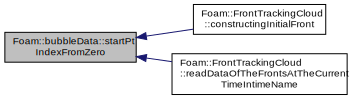
\includegraphics[width=350pt]{classFoam_1_1bubbleData_a01a4a0bd51dfdfd148cd09f173c42443_icgraph}
\end{center}
\end{figure}
\mbox{\Hypertarget{classFoam_1_1bubbleData_aeca8b64dfc956cf92b07fc98de0b1fb3}\label{classFoam_1_1bubbleData_aeca8b64dfc956cf92b07fc98de0b1fb3}} 
\index{Foam\+::bubble\+Data@{Foam\+::bubble\+Data}!update\+Bubble\+Surface@{update\+Bubble\+Surface}}
\index{update\+Bubble\+Surface@{update\+Bubble\+Surface}!Foam\+::bubble\+Data@{Foam\+::bubble\+Data}}
\subsubsection{\texorpdfstring{update\+Bubble\+Surface()}{updateBubbleSurface()}\hspace{0.1cm}{\footnotesize\ttfamily [1/2]}}
{\footnotesize\ttfamily void Foam\+::bubble\+Data\+::update\+Bubble\+Surface (\begin{DoxyParamCaption}{ }\end{DoxyParamCaption})\hspace{0.3cm}{\ttfamily [inline]}}

\mbox{\Hypertarget{classFoam_1_1bubbleData_aeca8b64dfc956cf92b07fc98de0b1fb3}\label{classFoam_1_1bubbleData_aeca8b64dfc956cf92b07fc98de0b1fb3}} 
\index{Foam\+::bubble\+Data@{Foam\+::bubble\+Data}!update\+Bubble\+Surface@{update\+Bubble\+Surface}}
\index{update\+Bubble\+Surface@{update\+Bubble\+Surface}!Foam\+::bubble\+Data@{Foam\+::bubble\+Data}}
\subsubsection{\texorpdfstring{update\+Bubble\+Surface()}{updateBubbleSurface()}\hspace{0.1cm}{\footnotesize\ttfamily [2/2]}}
{\footnotesize\ttfamily void Foam\+::bubble\+Data\+::update\+Bubble\+Surface (\begin{DoxyParamCaption}{ }\end{DoxyParamCaption})\hspace{0.3cm}{\ttfamily [inline]}}

Here is the call graph for this function\+:\nopagebreak
\begin{figure}[H]
\begin{center}
\leavevmode
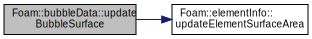
\includegraphics[width=350pt]{classFoam_1_1bubbleData_aeca8b64dfc956cf92b07fc98de0b1fb3_cgraph}
\end{center}
\end{figure}
Here is the caller graph for this function\+:\nopagebreak
\begin{figure}[H]
\begin{center}
\leavevmode
\includegraphics[width=350pt]{classFoam_1_1bubbleData_aeca8b64dfc956cf92b07fc98de0b1fb3_icgraph}
\end{center}
\end{figure}
\mbox{\Hypertarget{classFoam_1_1bubbleData_aa62a18b88be0327ed56c49a48cc2820b}\label{classFoam_1_1bubbleData_aa62a18b88be0327ed56c49a48cc2820b}} 
\index{Foam\+::bubble\+Data@{Foam\+::bubble\+Data}!update\+Bubble\+Volume@{update\+Bubble\+Volume}}
\index{update\+Bubble\+Volume@{update\+Bubble\+Volume}!Foam\+::bubble\+Data@{Foam\+::bubble\+Data}}
\subsubsection{\texorpdfstring{update\+Bubble\+Volume()}{updateBubbleVolume()}\hspace{0.1cm}{\footnotesize\ttfamily [1/2]}}
{\footnotesize\ttfamily void Foam\+::bubble\+Data\+::update\+Bubble\+Volume (\begin{DoxyParamCaption}{ }\end{DoxyParamCaption})\hspace{0.3cm}{\ttfamily [inline]}}

\mbox{\Hypertarget{classFoam_1_1bubbleData_aa62a18b88be0327ed56c49a48cc2820b}\label{classFoam_1_1bubbleData_aa62a18b88be0327ed56c49a48cc2820b}} 
\index{Foam\+::bubble\+Data@{Foam\+::bubble\+Data}!update\+Bubble\+Volume@{update\+Bubble\+Volume}}
\index{update\+Bubble\+Volume@{update\+Bubble\+Volume}!Foam\+::bubble\+Data@{Foam\+::bubble\+Data}}
\subsubsection{\texorpdfstring{update\+Bubble\+Volume()}{updateBubbleVolume()}\hspace{0.1cm}{\footnotesize\ttfamily [2/2]}}
{\footnotesize\ttfamily void Foam\+::bubble\+Data\+::update\+Bubble\+Volume (\begin{DoxyParamCaption}{ }\end{DoxyParamCaption})\hspace{0.3cm}{\ttfamily [inline]}}

Here is the caller graph for this function\+:\nopagebreak
\begin{figure}[H]
\begin{center}
\leavevmode
\includegraphics[width=350pt]{classFoam_1_1bubbleData_aa62a18b88be0327ed56c49a48cc2820b_icgraph}
\end{center}
\end{figure}


\subsection{Member Data Documentation}
\mbox{\Hypertarget{classFoam_1_1bubbleData_acd5cb743fe1daca143e57e30f6ef6487}\label{classFoam_1_1bubbleData_acd5cb743fe1daca143e57e30f6ef6487}} 
\index{Foam\+::bubble\+Data@{Foam\+::bubble\+Data}!accelaration@{accelaration}}
\index{accelaration@{accelaration}!Foam\+::bubble\+Data@{Foam\+::bubble\+Data}}
\subsubsection{\texorpdfstring{accelaration}{accelaration}}
{\footnotesize\ttfamily vector Foam\+::bubble\+Data\+::accelaration}

\mbox{\Hypertarget{classFoam_1_1bubbleData_a26444575af04c6f0b29a04fcc323e7b5}\label{classFoam_1_1bubbleData_a26444575af04c6f0b29a04fcc323e7b5}} 
\index{Foam\+::bubble\+Data@{Foam\+::bubble\+Data}!buoyant\+Force@{buoyant\+Force}}
\index{buoyant\+Force@{buoyant\+Force}!Foam\+::bubble\+Data@{Foam\+::bubble\+Data}}
\subsubsection{\texorpdfstring{buoyant\+Force}{buoyantForce}}
{\footnotesize\ttfamily vector Foam\+::bubble\+Data\+::buoyant\+Force}

\mbox{\Hypertarget{classFoam_1_1bubbleData_a71a1e15224b7eac3f2411eba31f9b245}\label{classFoam_1_1bubbleData_a71a1e15224b7eac3f2411eba31f9b245}} 
\index{Foam\+::bubble\+Data@{Foam\+::bubble\+Data}!centre@{centre}}
\index{centre@{centre}!Foam\+::bubble\+Data@{Foam\+::bubble\+Data}}
\subsubsection{\texorpdfstring{centre}{centre}}
{\footnotesize\ttfamily vector Foam\+::bubble\+Data\+::centre}

\mbox{\Hypertarget{classFoam_1_1bubbleData_a07eabe2600aba9ae1b8f8722baa2e929}\label{classFoam_1_1bubbleData_a07eabe2600aba9ae1b8f8722baa2e929}} 
\index{Foam\+::bubble\+Data@{Foam\+::bubble\+Data}!centre\+Old@{centre\+Old}}
\index{centre\+Old@{centre\+Old}!Foam\+::bubble\+Data@{Foam\+::bubble\+Data}}
\subsubsection{\texorpdfstring{centre\+Old}{centreOld}}
{\footnotesize\ttfamily vector Foam\+::bubble\+Data\+::centre\+Old}

\mbox{\Hypertarget{classFoam_1_1bubbleData_afab8b5aa167b02470788d3f3d4b3d7cd}\label{classFoam_1_1bubbleData_afab8b5aa167b02470788d3f3d4b3d7cd}} 
\index{Foam\+::bubble\+Data@{Foam\+::bubble\+Data}!current\+Index@{current\+Index}}
\index{current\+Index@{current\+Index}!Foam\+::bubble\+Data@{Foam\+::bubble\+Data}}
\subsubsection{\texorpdfstring{current\+Index}{currentIndex}}
{\footnotesize\ttfamily label Foam\+::bubble\+Data\+::current\+Index}

\mbox{\Hypertarget{classFoam_1_1bubbleData_a35633f81703ca31b7b06cdbc51218991}\label{classFoam_1_1bubbleData_a35633f81703ca31b7b06cdbc51218991}} 
\index{Foam\+::bubble\+Data@{Foam\+::bubble\+Data}!density@{density}}
\index{density@{density}!Foam\+::bubble\+Data@{Foam\+::bubble\+Data}}
\subsubsection{\texorpdfstring{density}{density}}
{\footnotesize\ttfamily scalar Foam\+::bubble\+Data\+::density}

\mbox{\Hypertarget{classFoam_1_1bubbleData_a2bf3e3d90a32e574d289d88ff5b2f2ed}\label{classFoam_1_1bubbleData_a2bf3e3d90a32e574d289d88ff5b2f2ed}} 
\index{Foam\+::bubble\+Data@{Foam\+::bubble\+Data}!diameter@{diameter}}
\index{diameter@{diameter}!Foam\+::bubble\+Data@{Foam\+::bubble\+Data}}
\subsubsection{\texorpdfstring{diameter}{diameter}}
{\footnotesize\ttfamily List$<$ scalar $>$ Foam\+::bubble\+Data\+::diameter}

\mbox{\Hypertarget{classFoam_1_1bubbleData_add40c043c47fac7ac16bff1e03823dca}\label{classFoam_1_1bubbleData_add40c043c47fac7ac16bff1e03823dca}} 
\index{Foam\+::bubble\+Data@{Foam\+::bubble\+Data}!drag\+Coeff@{drag\+Coeff}}
\index{drag\+Coeff@{drag\+Coeff}!Foam\+::bubble\+Data@{Foam\+::bubble\+Data}}
\subsubsection{\texorpdfstring{drag\+Coeff}{dragCoeff}}
{\footnotesize\ttfamily scalar Foam\+::bubble\+Data\+::drag\+Coeff}

\mbox{\Hypertarget{classFoam_1_1bubbleData_a8b56f8139f82c448103b2f8296be3587}\label{classFoam_1_1bubbleData_a8b56f8139f82c448103b2f8296be3587}} 
\index{Foam\+::bubble\+Data@{Foam\+::bubble\+Data}!eL@{eL}}
\index{eL@{eL}!Foam\+::bubble\+Data@{Foam\+::bubble\+Data}}
\subsubsection{\texorpdfstring{eL}{eL}}
{\footnotesize\ttfamily Dynamic\+List$<$ \hyperlink{classFoam_1_1elementInfo}{element\+Info} $>$ Foam\+::bubble\+Data\+::eL}

\mbox{\Hypertarget{classFoam_1_1bubbleData_ae0a6387d9d99d4d6ce94e0ccb265f5d2}\label{classFoam_1_1bubbleData_ae0a6387d9d99d4d6ce94e0ccb265f5d2}} 
\index{Foam\+::bubble\+Data@{Foam\+::bubble\+Data}!el\+C\+Pos\+In\+Domain\+Flag@{el\+C\+Pos\+In\+Domain\+Flag}}
\index{el\+C\+Pos\+In\+Domain\+Flag@{el\+C\+Pos\+In\+Domain\+Flag}!Foam\+::bubble\+Data@{Foam\+::bubble\+Data}}
\subsubsection{\texorpdfstring{el\+C\+Pos\+In\+Domain\+Flag}{elCPosInDomainFlag}}
{\footnotesize\ttfamily bool Foam\+::bubble\+Data\+::el\+C\+Pos\+In\+Domain\+Flag}

\mbox{\Hypertarget{classFoam_1_1bubbleData_a9d67f3633db9de211d0a8bf4d6a70fd8}\label{classFoam_1_1bubbleData_a9d67f3633db9de211d0a8bf4d6a70fd8}} 
\index{Foam\+::bubble\+Data@{Foam\+::bubble\+Data}!el\+Neighbor\+Flag@{el\+Neighbor\+Flag}}
\index{el\+Neighbor\+Flag@{el\+Neighbor\+Flag}!Foam\+::bubble\+Data@{Foam\+::bubble\+Data}}
\subsubsection{\texorpdfstring{el\+Neighbor\+Flag}{elNeighborFlag}}
{\footnotesize\ttfamily bool Foam\+::bubble\+Data\+::el\+Neighbor\+Flag}

\mbox{\Hypertarget{classFoam_1_1bubbleData_aefeccb5501bc3d113b6fef02a3ea2bae}\label{classFoam_1_1bubbleData_aefeccb5501bc3d113b6fef02a3ea2bae}} 
\index{Foam\+::bubble\+Data@{Foam\+::bubble\+Data}!el\+Points\+Flag@{el\+Points\+Flag}}
\index{el\+Points\+Flag@{el\+Points\+Flag}!Foam\+::bubble\+Data@{Foam\+::bubble\+Data}}
\subsubsection{\texorpdfstring{el\+Points\+Flag}{elPointsFlag}}
{\footnotesize\ttfamily bool Foam\+::bubble\+Data\+::el\+Points\+Flag}

\mbox{\Hypertarget{classFoam_1_1bubbleData_acf7c9565ddd9cc8235769a19707b3451}\label{classFoam_1_1bubbleData_acf7c9565ddd9cc8235769a19707b3451}} 
\index{Foam\+::bubble\+Data@{Foam\+::bubble\+Data}!el\+Surface\+Flag@{el\+Surface\+Flag}}
\index{el\+Surface\+Flag@{el\+Surface\+Flag}!Foam\+::bubble\+Data@{Foam\+::bubble\+Data}}
\subsubsection{\texorpdfstring{el\+Surface\+Flag}{elSurfaceFlag}}
{\footnotesize\ttfamily bool Foam\+::bubble\+Data\+::el\+Surface\+Flag}

\mbox{\Hypertarget{classFoam_1_1bubbleData_a6256640184e8fe3c9e55aade352ea782}\label{classFoam_1_1bubbleData_a6256640184e8fe3c9e55aade352ea782}} 
\index{Foam\+::bubble\+Data@{Foam\+::bubble\+Data}!Eotvos\+Number@{Eotvos\+Number}}
\index{Eotvos\+Number@{Eotvos\+Number}!Foam\+::bubble\+Data@{Foam\+::bubble\+Data}}
\subsubsection{\texorpdfstring{Eotvos\+Number}{EotvosNumber}}
{\footnotesize\ttfamily scalar Foam\+::bubble\+Data\+::\+Eotvos\+Number}

\mbox{\Hypertarget{classFoam_1_1bubbleData_ab0498b3d44aa2e83e63c60de8a2dcefa}\label{classFoam_1_1bubbleData_ab0498b3d44aa2e83e63c60de8a2dcefa}} 
\index{Foam\+::bubble\+Data@{Foam\+::bubble\+Data}!friction\+Drag\+Force@{friction\+Drag\+Force}}
\index{friction\+Drag\+Force@{friction\+Drag\+Force}!Foam\+::bubble\+Data@{Foam\+::bubble\+Data}}
\subsubsection{\texorpdfstring{friction\+Drag\+Force}{frictionDragForce}}
{\footnotesize\ttfamily scalar Foam\+::bubble\+Data\+::friction\+Drag\+Force}

\mbox{\Hypertarget{classFoam_1_1bubbleData_aba3c36d8dee4a54fd00e7f03c0e99b3e}\label{classFoam_1_1bubbleData_aba3c36d8dee4a54fd00e7f03c0e99b3e}} 
\index{Foam\+::bubble\+Data@{Foam\+::bubble\+Data}!friction\+Lift\+ForceI@{friction\+Lift\+ForceI}}
\index{friction\+Lift\+ForceI@{friction\+Lift\+ForceI}!Foam\+::bubble\+Data@{Foam\+::bubble\+Data}}
\subsubsection{\texorpdfstring{friction\+Lift\+ForceI}{frictionLiftForceI}}
{\footnotesize\ttfamily scalar Foam\+::bubble\+Data\+::friction\+Lift\+ForceI}

\mbox{\Hypertarget{classFoam_1_1bubbleData_a611eb9b38cad5263f53ae226ab5af33b}\label{classFoam_1_1bubbleData_a611eb9b38cad5263f53ae226ab5af33b}} 
\index{Foam\+::bubble\+Data@{Foam\+::bubble\+Data}!friction\+Lift\+Force\+II@{friction\+Lift\+Force\+II}}
\index{friction\+Lift\+Force\+II@{friction\+Lift\+Force\+II}!Foam\+::bubble\+Data@{Foam\+::bubble\+Data}}
\subsubsection{\texorpdfstring{friction\+Lift\+Force\+II}{frictionLiftForceII}}
{\footnotesize\ttfamily scalar Foam\+::bubble\+Data\+::friction\+Lift\+Force\+II}

\mbox{\Hypertarget{classFoam_1_1bubbleData_a377d050bf5cccc31cb1842a7471f0b40}\label{classFoam_1_1bubbleData_a377d050bf5cccc31cb1842a7471f0b40}} 
\index{Foam\+::bubble\+Data@{Foam\+::bubble\+Data}!gravity\+Force@{gravity\+Force}}
\index{gravity\+Force@{gravity\+Force}!Foam\+::bubble\+Data@{Foam\+::bubble\+Data}}
\subsubsection{\texorpdfstring{gravity\+Force}{gravityForce}}
{\footnotesize\ttfamily vector Foam\+::bubble\+Data\+::gravity\+Force}

\mbox{\Hypertarget{classFoam_1_1bubbleData_aa40fd779e46229fc8c402c46d75fad8d}\label{classFoam_1_1bubbleData_aa40fd779e46229fc8c402c46d75fad8d}} 
\index{Foam\+::bubble\+Data@{Foam\+::bubble\+Data}!keep\+Bubble@{keep\+Bubble}}
\index{keep\+Bubble@{keep\+Bubble}!Foam\+::bubble\+Data@{Foam\+::bubble\+Data}}
\subsubsection{\texorpdfstring{keep\+Bubble}{keepBubble}}
{\footnotesize\ttfamily bool Foam\+::bubble\+Data\+::keep\+Bubble}

\mbox{\Hypertarget{classFoam_1_1bubbleData_ada8e7f1dc0b9a282f63a8a777a70cef5}\label{classFoam_1_1bubbleData_ada8e7f1dc0b9a282f63a8a777a70cef5}} 
\index{Foam\+::bubble\+Data@{Foam\+::bubble\+Data}!Lift\+CoeffI@{Lift\+CoeffI}}
\index{Lift\+CoeffI@{Lift\+CoeffI}!Foam\+::bubble\+Data@{Foam\+::bubble\+Data}}
\subsubsection{\texorpdfstring{Lift\+CoeffI}{LiftCoeffI}}
{\footnotesize\ttfamily scalar Foam\+::bubble\+Data\+::\+Lift\+CoeffI}

\mbox{\Hypertarget{classFoam_1_1bubbleData_a7bad7043d9e915dd6aabc47608b114e5}\label{classFoam_1_1bubbleData_a7bad7043d9e915dd6aabc47608b114e5}} 
\index{Foam\+::bubble\+Data@{Foam\+::bubble\+Data}!Lift\+Coeff\+II@{Lift\+Coeff\+II}}
\index{Lift\+Coeff\+II@{Lift\+Coeff\+II}!Foam\+::bubble\+Data@{Foam\+::bubble\+Data}}
\subsubsection{\texorpdfstring{Lift\+Coeff\+II}{LiftCoeffII}}
{\footnotesize\ttfamily scalar Foam\+::bubble\+Data\+::\+Lift\+Coeff\+II}

\mbox{\Hypertarget{classFoam_1_1bubbleData_a956a6ca9a5125d1b0ccb94bd2487ca29}\label{classFoam_1_1bubbleData_a956a6ca9a5125d1b0ccb94bd2487ca29}} 
\index{Foam\+::bubble\+Data@{Foam\+::bubble\+Data}!mass@{mass}}
\index{mass@{mass}!Foam\+::bubble\+Data@{Foam\+::bubble\+Data}}
\subsubsection{\texorpdfstring{mass}{mass}}
{\footnotesize\ttfamily scalar Foam\+::bubble\+Data\+::mass}

\mbox{\Hypertarget{classFoam_1_1bubbleData_af3720d63ef807c83c099b3ad7dd77f5d}\label{classFoam_1_1bubbleData_af3720d63ef807c83c099b3ad7dd77f5d}} 
\index{Foam\+::bubble\+Data@{Foam\+::bubble\+Data}!Morton\+Number@{Morton\+Number}}
\index{Morton\+Number@{Morton\+Number}!Foam\+::bubble\+Data@{Foam\+::bubble\+Data}}
\subsubsection{\texorpdfstring{Morton\+Number}{MortonNumber}}
{\footnotesize\ttfamily scalar Foam\+::bubble\+Data\+::\+Morton\+Number}

\mbox{\Hypertarget{classFoam_1_1bubbleData_a181098e2c93266f0b4c6861522b478b3}\label{classFoam_1_1bubbleData_a181098e2c93266f0b4c6861522b478b3}} 
\index{Foam\+::bubble\+Data@{Foam\+::bubble\+Data}!outer\+Fluid\+Density@{outer\+Fluid\+Density}}
\index{outer\+Fluid\+Density@{outer\+Fluid\+Density}!Foam\+::bubble\+Data@{Foam\+::bubble\+Data}}
\subsubsection{\texorpdfstring{outer\+Fluid\+Density}{outerFluidDensity}}
{\footnotesize\ttfamily scalar Foam\+::bubble\+Data\+::outer\+Fluid\+Density}

\mbox{\Hypertarget{classFoam_1_1bubbleData_a20908303d8e37f882e52595d1da9beb1}\label{classFoam_1_1bubbleData_a20908303d8e37f882e52595d1da9beb1}} 
\index{Foam\+::bubble\+Data@{Foam\+::bubble\+Data}!outer\+Fluid\+Viscosity@{outer\+Fluid\+Viscosity}}
\index{outer\+Fluid\+Viscosity@{outer\+Fluid\+Viscosity}!Foam\+::bubble\+Data@{Foam\+::bubble\+Data}}
\subsubsection{\texorpdfstring{outer\+Fluid\+Viscosity}{outerFluidViscosity}}
{\footnotesize\ttfamily scalar Foam\+::bubble\+Data\+::outer\+Fluid\+Viscosity}

\mbox{\Hypertarget{classFoam_1_1bubbleData_a466b40438d465e522c6cf9b6ae042638}\label{classFoam_1_1bubbleData_a466b40438d465e522c6cf9b6ae042638}} 
\index{Foam\+::bubble\+Data@{Foam\+::bubble\+Data}!pL@{pL}}
\index{pL@{pL}!Foam\+::bubble\+Data@{Foam\+::bubble\+Data}}
\subsubsection{\texorpdfstring{pL}{pL}}
{\footnotesize\ttfamily Dynamic\+List$<$ \hyperlink{classFoam_1_1pointData}{point\+Data} $>$ Foam\+::bubble\+Data\+::pL}

\mbox{\Hypertarget{classFoam_1_1bubbleData_a15e8c5d0bd3a677e2d81c2b4ebe50dea}\label{classFoam_1_1bubbleData_a15e8c5d0bd3a677e2d81c2b4ebe50dea}} 
\index{Foam\+::bubble\+Data@{Foam\+::bubble\+Data}!pl\+Connection\+Flag@{pl\+Connection\+Flag}}
\index{pl\+Connection\+Flag@{pl\+Connection\+Flag}!Foam\+::bubble\+Data@{Foam\+::bubble\+Data}}
\subsubsection{\texorpdfstring{pl\+Connection\+Flag}{plConnectionFlag}}
{\footnotesize\ttfamily bool Foam\+::bubble\+Data\+::pl\+Connection\+Flag}

\mbox{\Hypertarget{classFoam_1_1bubbleData_aa9c8dd1bfe64b2f19dc441d87b888d9c}\label{classFoam_1_1bubbleData_aa9c8dd1bfe64b2f19dc441d87b888d9c}} 
\index{Foam\+::bubble\+Data@{Foam\+::bubble\+Data}!p\+L\+Pos\+In\+Domain\+Flag@{p\+L\+Pos\+In\+Domain\+Flag}}
\index{p\+L\+Pos\+In\+Domain\+Flag@{p\+L\+Pos\+In\+Domain\+Flag}!Foam\+::bubble\+Data@{Foam\+::bubble\+Data}}
\subsubsection{\texorpdfstring{p\+L\+Pos\+In\+Domain\+Flag}{pLPosInDomainFlag}}
{\footnotesize\ttfamily bool Foam\+::bubble\+Data\+::p\+L\+Pos\+In\+Domain\+Flag}

\mbox{\Hypertarget{classFoam_1_1bubbleData_abf4def2ca2031f32ef6d3d9039fe659b}\label{classFoam_1_1bubbleData_abf4def2ca2031f32ef6d3d9039fe659b}} 
\index{Foam\+::bubble\+Data@{Foam\+::bubble\+Data}!pressure\+Drag\+Force@{pressure\+Drag\+Force}}
\index{pressure\+Drag\+Force@{pressure\+Drag\+Force}!Foam\+::bubble\+Data@{Foam\+::bubble\+Data}}
\subsubsection{\texorpdfstring{pressure\+Drag\+Force}{pressureDragForce}}
{\footnotesize\ttfamily scalar Foam\+::bubble\+Data\+::pressure\+Drag\+Force}

\mbox{\Hypertarget{classFoam_1_1bubbleData_a0a3b90c342d0c81cce02aa50fe650b4f}\label{classFoam_1_1bubbleData_a0a3b90c342d0c81cce02aa50fe650b4f}} 
\index{Foam\+::bubble\+Data@{Foam\+::bubble\+Data}!pressure\+Force@{pressure\+Force}}
\index{pressure\+Force@{pressure\+Force}!Foam\+::bubble\+Data@{Foam\+::bubble\+Data}}
\subsubsection{\texorpdfstring{pressure\+Force}{pressureForce}}
{\footnotesize\ttfamily vector Foam\+::bubble\+Data\+::pressure\+Force}

\mbox{\Hypertarget{classFoam_1_1bubbleData_a9f920dfaf0d1f9da22207d08b8e1cbc1}\label{classFoam_1_1bubbleData_a9f920dfaf0d1f9da22207d08b8e1cbc1}} 
\index{Foam\+::bubble\+Data@{Foam\+::bubble\+Data}!pressure\+Jump\+At\+The\+Interface@{pressure\+Jump\+At\+The\+Interface}}
\index{pressure\+Jump\+At\+The\+Interface@{pressure\+Jump\+At\+The\+Interface}!Foam\+::bubble\+Data@{Foam\+::bubble\+Data}}
\subsubsection{\texorpdfstring{pressure\+Jump\+At\+The\+Interface}{pressureJumpAtTheInterface}}
{\footnotesize\ttfamily vector Foam\+::bubble\+Data\+::pressure\+Jump\+At\+The\+Interface}

\mbox{\Hypertarget{classFoam_1_1bubbleData_a3c93a65a6c6d39068229947c01c7d06d}\label{classFoam_1_1bubbleData_a3c93a65a6c6d39068229947c01c7d06d}} 
\index{Foam\+::bubble\+Data@{Foam\+::bubble\+Data}!pressure\+Lift\+ForceI@{pressure\+Lift\+ForceI}}
\index{pressure\+Lift\+ForceI@{pressure\+Lift\+ForceI}!Foam\+::bubble\+Data@{Foam\+::bubble\+Data}}
\subsubsection{\texorpdfstring{pressure\+Lift\+ForceI}{pressureLiftForceI}}
{\footnotesize\ttfamily scalar Foam\+::bubble\+Data\+::pressure\+Lift\+ForceI}

\mbox{\Hypertarget{classFoam_1_1bubbleData_a9ab24dd7989a030ca7c038336bdfcec9}\label{classFoam_1_1bubbleData_a9ab24dd7989a030ca7c038336bdfcec9}} 
\index{Foam\+::bubble\+Data@{Foam\+::bubble\+Data}!pressure\+Lift\+Force\+II@{pressure\+Lift\+Force\+II}}
\index{pressure\+Lift\+Force\+II@{pressure\+Lift\+Force\+II}!Foam\+::bubble\+Data@{Foam\+::bubble\+Data}}
\subsubsection{\texorpdfstring{pressure\+Lift\+Force\+II}{pressureLiftForceII}}
{\footnotesize\ttfamily scalar Foam\+::bubble\+Data\+::pressure\+Lift\+Force\+II}

\mbox{\Hypertarget{classFoam_1_1bubbleData_af3b01e31394ca2db56831b637c823fad}\label{classFoam_1_1bubbleData_af3b01e31394ca2db56831b637c823fad}} 
\index{Foam\+::bubble\+Data@{Foam\+::bubble\+Data}!shear\+Stress\+Force@{shear\+Stress\+Force}}
\index{shear\+Stress\+Force@{shear\+Stress\+Force}!Foam\+::bubble\+Data@{Foam\+::bubble\+Data}}
\subsubsection{\texorpdfstring{shear\+Stress\+Force}{shearStressForce}}
{\footnotesize\ttfamily vector Foam\+::bubble\+Data\+::shear\+Stress\+Force}

\mbox{\Hypertarget{classFoam_1_1bubbleData_a0427ab63bc536b2b2ac8b0e372828f5e}\label{classFoam_1_1bubbleData_a0427ab63bc536b2b2ac8b0e372828f5e}} 
\index{Foam\+::bubble\+Data@{Foam\+::bubble\+Data}!sphere\+Bubble\+Diameter@{sphere\+Bubble\+Diameter}}
\index{sphere\+Bubble\+Diameter@{sphere\+Bubble\+Diameter}!Foam\+::bubble\+Data@{Foam\+::bubble\+Data}}
\subsubsection{\texorpdfstring{sphere\+Bubble\+Diameter}{sphereBubbleDiameter}}
{\footnotesize\ttfamily scalar Foam\+::bubble\+Data\+::sphere\+Bubble\+Diameter}

\mbox{\Hypertarget{classFoam_1_1bubbleData_a7ba3dffa9c8bf20077966d44c2a3fd9d}\label{classFoam_1_1bubbleData_a7ba3dffa9c8bf20077966d44c2a3fd9d}} 
\index{Foam\+::bubble\+Data@{Foam\+::bubble\+Data}!sphericity@{sphericity}}
\index{sphericity@{sphericity}!Foam\+::bubble\+Data@{Foam\+::bubble\+Data}}
\subsubsection{\texorpdfstring{sphericity}{sphericity}}
{\footnotesize\ttfamily scalar Foam\+::bubble\+Data\+::sphericity}

\mbox{\Hypertarget{classFoam_1_1bubbleData_afa34821682366185de9b87a483dd6f43}\label{classFoam_1_1bubbleData_afa34821682366185de9b87a483dd6f43}} 
\index{Foam\+::bubble\+Data@{Foam\+::bubble\+Data}!surface\+Area@{surface\+Area}}
\index{surface\+Area@{surface\+Area}!Foam\+::bubble\+Data@{Foam\+::bubble\+Data}}
\subsubsection{\texorpdfstring{surface\+Area}{surfaceArea}}
{\footnotesize\ttfamily scalar Foam\+::bubble\+Data\+::surface\+Area}

\mbox{\Hypertarget{classFoam_1_1bubbleData_aec394160aa23b63eb672846179287f8e}\label{classFoam_1_1bubbleData_aec394160aa23b63eb672846179287f8e}} 
\index{Foam\+::bubble\+Data@{Foam\+::bubble\+Data}!surface\+Tension\+Coeff@{surface\+Tension\+Coeff}}
\index{surface\+Tension\+Coeff@{surface\+Tension\+Coeff}!Foam\+::bubble\+Data@{Foam\+::bubble\+Data}}
\subsubsection{\texorpdfstring{surface\+Tension\+Coeff}{surfaceTensionCoeff}}
{\footnotesize\ttfamily scalar Foam\+::bubble\+Data\+::surface\+Tension\+Coeff}

\mbox{\Hypertarget{classFoam_1_1bubbleData_a37593f268513154da15399f5d346161a}\label{classFoam_1_1bubbleData_a37593f268513154da15399f5d346161a}} 
\index{Foam\+::bubble\+Data@{Foam\+::bubble\+Data}!total\+Drag\+Force@{total\+Drag\+Force}}
\index{total\+Drag\+Force@{total\+Drag\+Force}!Foam\+::bubble\+Data@{Foam\+::bubble\+Data}}
\subsubsection{\texorpdfstring{total\+Drag\+Force}{totalDragForce}}
{\footnotesize\ttfamily scalar Foam\+::bubble\+Data\+::total\+Drag\+Force}

\mbox{\Hypertarget{classFoam_1_1bubbleData_a46b4565cc9a62aa11f8ababc548115d8}\label{classFoam_1_1bubbleData_a46b4565cc9a62aa11f8ababc548115d8}} 
\index{Foam\+::bubble\+Data@{Foam\+::bubble\+Data}!total\+Lift\+ForceI@{total\+Lift\+ForceI}}
\index{total\+Lift\+ForceI@{total\+Lift\+ForceI}!Foam\+::bubble\+Data@{Foam\+::bubble\+Data}}
\subsubsection{\texorpdfstring{total\+Lift\+ForceI}{totalLiftForceI}}
{\footnotesize\ttfamily scalar Foam\+::bubble\+Data\+::total\+Lift\+ForceI}

\mbox{\Hypertarget{classFoam_1_1bubbleData_af405b224178a16813fed947591cb1bff}\label{classFoam_1_1bubbleData_af405b224178a16813fed947591cb1bff}} 
\index{Foam\+::bubble\+Data@{Foam\+::bubble\+Data}!total\+Lift\+Force\+II@{total\+Lift\+Force\+II}}
\index{total\+Lift\+Force\+II@{total\+Lift\+Force\+II}!Foam\+::bubble\+Data@{Foam\+::bubble\+Data}}
\subsubsection{\texorpdfstring{total\+Lift\+Force\+II}{totalLiftForceII}}
{\footnotesize\ttfamily scalar Foam\+::bubble\+Data\+::total\+Lift\+Force\+II}

\mbox{\Hypertarget{classFoam_1_1bubbleData_a6f24e8e0d7d406bc0fce92c61c7b9f6a}\label{classFoam_1_1bubbleData_a6f24e8e0d7d406bc0fce92c61c7b9f6a}} 
\index{Foam\+::bubble\+Data@{Foam\+::bubble\+Data}!velocity@{velocity}}
\index{velocity@{velocity}!Foam\+::bubble\+Data@{Foam\+::bubble\+Data}}
\subsubsection{\texorpdfstring{velocity}{velocity}}
{\footnotesize\ttfamily vector Foam\+::bubble\+Data\+::velocity}

\mbox{\Hypertarget{classFoam_1_1bubbleData_a2ddfba5a0c373cf04288b484a3f20b1e}\label{classFoam_1_1bubbleData_a2ddfba5a0c373cf04288b484a3f20b1e}} 
\index{Foam\+::bubble\+Data@{Foam\+::bubble\+Data}!velocity\+Old@{velocity\+Old}}
\index{velocity\+Old@{velocity\+Old}!Foam\+::bubble\+Data@{Foam\+::bubble\+Data}}
\subsubsection{\texorpdfstring{velocity\+Old}{velocityOld}}
{\footnotesize\ttfamily vector Foam\+::bubble\+Data\+::velocity\+Old}

\mbox{\Hypertarget{classFoam_1_1bubbleData_a82b5b5338bb0d363e79e8078d84fbdaf}\label{classFoam_1_1bubbleData_a82b5b5338bb0d363e79e8078d84fbdaf}} 
\index{Foam\+::bubble\+Data@{Foam\+::bubble\+Data}!viscosity@{viscosity}}
\index{viscosity@{viscosity}!Foam\+::bubble\+Data@{Foam\+::bubble\+Data}}
\subsubsection{\texorpdfstring{viscosity}{viscosity}}
{\footnotesize\ttfamily scalar Foam\+::bubble\+Data\+::viscosity}

\mbox{\Hypertarget{classFoam_1_1bubbleData_af26ac17dd3c8484703b484b1a0b406f6}\label{classFoam_1_1bubbleData_af26ac17dd3c8484703b484b1a0b406f6}} 
\index{Foam\+::bubble\+Data@{Foam\+::bubble\+Data}!volume@{volume}}
\index{volume@{volume}!Foam\+::bubble\+Data@{Foam\+::bubble\+Data}}
\subsubsection{\texorpdfstring{volume}{volume}}
{\footnotesize\ttfamily scalar Foam\+::bubble\+Data\+::volume}

\mbox{\Hypertarget{classFoam_1_1bubbleData_a8542e54692c07cedc2c0cae2a74ba24d}\label{classFoam_1_1bubbleData_a8542e54692c07cedc2c0cae2a74ba24d}} 
\index{Foam\+::bubble\+Data@{Foam\+::bubble\+Data}!volume0@{volume0}}
\index{volume0@{volume0}!Foam\+::bubble\+Data@{Foam\+::bubble\+Data}}
\subsubsection{\texorpdfstring{volume0}{volume0}}
{\footnotesize\ttfamily scalar Foam\+::bubble\+Data\+::volume0}

\mbox{\Hypertarget{classFoam_1_1bubbleData_ae83882aee8f42d1d3e3fd1c42610beb6}\label{classFoam_1_1bubbleData_ae83882aee8f42d1d3e3fd1c42610beb6}} 
\index{Foam\+::bubble\+Data@{Foam\+::bubble\+Data}!volume\+Flag@{volume\+Flag}}
\index{volume\+Flag@{volume\+Flag}!Foam\+::bubble\+Data@{Foam\+::bubble\+Data}}
\subsubsection{\texorpdfstring{volume\+Flag}{volumeFlag}}
{\footnotesize\ttfamily bool Foam\+::bubble\+Data\+::volume\+Flag}



The documentation for this class was generated from the following files\+:\begin{DoxyCompactItemize}
\item 
clouds/\+Templates/\+Front\+Tracking\+Cloud/bubble\+Data/\hyperlink{clouds_2Templates_2FrontTrackingCloud_2bubbleData_2bubbleData_8H}{bubble\+Data.\+H}\item 
clouds/\+Templates/\+Front\+Tracking\+Cloud/bubble\+Data/\hyperlink{clouds_2Templates_2FrontTrackingCloud_2bubbleData_2bubbleData_8C}{bubble\+Data.\+C}\item 
clouds/\+Templates/\+Front\+Tracking\+Cloud/bubble\+Data/\hyperlink{clouds_2Templates_2FrontTrackingCloud_2bubbleData_2bubbleDataI_8H}{bubble\+Data\+I.\+H}\end{DoxyCompactItemize}

\hypertarget{classFoam_1_1FrontToFieldModels_1_1CPT}{}\section{Foam\+:\+:Front\+To\+Field\+Models\+:\+:C\+PT$<$ Cloud\+Type $>$ Class Template Reference}
\label{classFoam_1_1FrontToFieldModels_1_1CPT}\index{Foam\+::\+Front\+To\+Field\+Models\+::\+C\+P\+T$<$ Cloud\+Type $>$@{Foam\+::\+Front\+To\+Field\+Models\+::\+C\+P\+T$<$ Cloud\+Type $>$}}


{\ttfamily \#include $<$C\+P\+T.\+H$>$}



Inheritance diagram for Foam\+:\+:Front\+To\+Field\+Models\+:\+:C\+PT$<$ Cloud\+Type $>$\+:\nopagebreak
\begin{figure}[H]
\begin{center}
\leavevmode
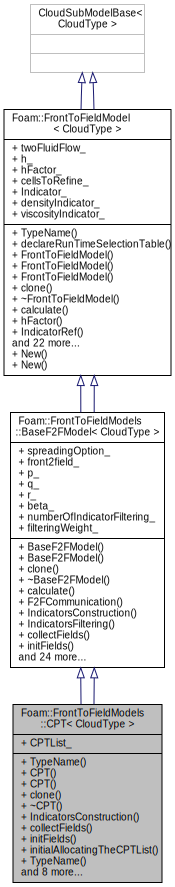
\includegraphics[height=550pt]{classFoam_1_1FrontToFieldModels_1_1CPT__inherit__graph}
\end{center}
\end{figure}


Collaboration diagram for Foam\+:\+:Front\+To\+Field\+Models\+:\+:C\+PT$<$ Cloud\+Type $>$\+:\nopagebreak
\begin{figure}[H]
\begin{center}
\leavevmode
\includegraphics[height=550pt]{classFoam_1_1FrontToFieldModels_1_1CPT__coll__graph}
\end{center}
\end{figure}
\subsection*{Classes}
\begin{DoxyCompactItemize}
\item 
class \hyperlink{classFoam_1_1FrontToFieldModels_1_1CPT_1_1CPTData}{C\+P\+T\+Data}
\end{DoxyCompactItemize}
\subsection*{Public Member Functions}
\begin{DoxyCompactItemize}
\item 
\hyperlink{classFoam_1_1FrontToFieldModels_1_1CPT_a288cadbe2779addeaf65f4994bb8f465}{Type\+Name} (\char`\"{}cpt\char`\"{})
\item 
\hyperlink{classFoam_1_1FrontToFieldModels_1_1CPT_afa4bdc286c92aa5ab5cbcb996c77e645}{C\+PT} (const dictionary \&dict, Cloud\+Type \&owner)
\item 
\hyperlink{classFoam_1_1FrontToFieldModels_1_1CPT_a0c392dba5bd5ecc9e060bd934b1e9e8d}{C\+PT} (const \hyperlink{classFoam_1_1FrontToFieldModels_1_1CPT}{C\+PT}$<$ Cloud\+Type $>$ \&cm)
\item 
virtual auto\+Ptr$<$ \hyperlink{classFoam_1_1FrontToFieldModel}{Front\+To\+Field\+Model}$<$ Cloud\+Type $>$ $>$ \hyperlink{classFoam_1_1FrontToFieldModels_1_1CPT_a1ba03c46bac4bba07f9ee8185baff1e6}{clone} () const
\item 
virtual \hyperlink{classFoam_1_1FrontToFieldModels_1_1CPT_a4d20832e3ec799dd9b18c76c27083fc6}{$\sim$\+C\+PT} ()
\item 
virtual void \hyperlink{classFoam_1_1FrontToFieldModels_1_1CPT_a8c38f2d1f3cad1e29d337ad43ca05309}{Indicators\+Construction} ()
\item 
virtual void \hyperlink{classFoam_1_1FrontToFieldModels_1_1CPT_a30ebffabafd2b102fd189269ffa3be2a}{collect\+Fields} (label cellI, label b\+DI, scalar w\+Bar, vector el\+Area\+Vec)
\item 
virtual void \hyperlink{classFoam_1_1FrontToFieldModels_1_1CPT_a81f9b6cb7a4f16d31e87fbcff452800b}{init\+Fields} ()
\item 
void \hyperlink{classFoam_1_1FrontToFieldModels_1_1CPT_a6a2bc39ec3cf7a842515a5661c9f4584}{initial\+Allocating\+The\+C\+P\+T\+List} ()
\item 
\hyperlink{classFoam_1_1FrontToFieldModels_1_1CPT_a288cadbe2779addeaf65f4994bb8f465}{Type\+Name} (\char`\"{}cpt\char`\"{})
\item 
\hyperlink{classFoam_1_1FrontToFieldModels_1_1CPT_afa4bdc286c92aa5ab5cbcb996c77e645}{C\+PT} (const dictionary \&dict, Cloud\+Type \&owner)
\item 
\hyperlink{classFoam_1_1FrontToFieldModels_1_1CPT_a0c392dba5bd5ecc9e060bd934b1e9e8d}{C\+PT} (const \hyperlink{classFoam_1_1FrontToFieldModels_1_1CPT}{C\+PT}$<$ Cloud\+Type $>$ \&cm)
\item 
virtual auto\+Ptr$<$ \hyperlink{classFoam_1_1FrontToFieldModel}{Front\+To\+Field\+Model}$<$ Cloud\+Type $>$ $>$ \hyperlink{classFoam_1_1FrontToFieldModels_1_1CPT_a1ba03c46bac4bba07f9ee8185baff1e6}{clone} () const
\item 
virtual \hyperlink{classFoam_1_1FrontToFieldModels_1_1CPT_af40de89dc82a59b880d3b4e7a05f62b6}{$\sim$\+C\+PT} ()
\item 
virtual void \hyperlink{classFoam_1_1FrontToFieldModels_1_1CPT_a3d1350ef9a447e3dbafa181f8195761c}{Indicators\+Construction} ()
\item 
virtual void \hyperlink{classFoam_1_1FrontToFieldModels_1_1CPT_ab2567f9d6b26e90f31c50c73cf62d32b}{collect\+Fields} (label cellI, label b\+DI, scalar w\+Bar, vector el\+Area\+Vec)
\item 
virtual void \hyperlink{classFoam_1_1FrontToFieldModels_1_1CPT_a051e181306632a5cc5fde3fdb7094c9a}{init\+Fields} ()
\item 
void \hyperlink{classFoam_1_1FrontToFieldModels_1_1CPT_ad44422a69564bdcf0cd2ead0015d9226}{initial\+Allocating\+The\+C\+P\+T\+List} ()
\end{DoxyCompactItemize}
\subsection*{Public Attributes}
\begin{DoxyCompactItemize}
\item 
List$<$ \hyperlink{classFoam_1_1FrontToFieldModels_1_1CPT_1_1CPTData}{C\+P\+T\+Data} $>$ \hyperlink{classFoam_1_1FrontToFieldModels_1_1CPT_acc46ef6b49688a927bc95b8967b1099b}{C\+P\+T\+List\+\_\+}
\end{DoxyCompactItemize}
\subsection*{Additional Inherited Members}


\subsection{Constructor \& Destructor Documentation}
\mbox{\Hypertarget{classFoam_1_1FrontToFieldModels_1_1CPT_afa4bdc286c92aa5ab5cbcb996c77e645}\label{classFoam_1_1FrontToFieldModels_1_1CPT_afa4bdc286c92aa5ab5cbcb996c77e645}} 
\index{Foam\+::\+Front\+To\+Field\+Models\+::\+C\+PT@{Foam\+::\+Front\+To\+Field\+Models\+::\+C\+PT}!C\+PT@{C\+PT}}
\index{C\+PT@{C\+PT}!Foam\+::\+Front\+To\+Field\+Models\+::\+C\+PT@{Foam\+::\+Front\+To\+Field\+Models\+::\+C\+PT}}
\subsubsection{\texorpdfstring{C\+P\+T()}{CPT()}\hspace{0.1cm}{\footnotesize\ttfamily [1/4]}}
{\footnotesize\ttfamily template$<$class Cloud\+Type $>$ \\
\hyperlink{classFoam_1_1FrontToFieldModels_1_1CPT}{Foam\+::\+Front\+To\+Field\+Models\+::\+C\+PT}$<$ Cloud\+Type $>$\+::\hyperlink{classFoam_1_1FrontToFieldModels_1_1CPT}{C\+PT} (\begin{DoxyParamCaption}\item[{const dictionary \&}]{dict,  }\item[{Cloud\+Type \&}]{owner }\end{DoxyParamCaption})}

Here is the caller graph for this function\+:\nopagebreak
\begin{figure}[H]
\begin{center}
\leavevmode
\includegraphics[width=350pt]{classFoam_1_1FrontToFieldModels_1_1CPT_afa4bdc286c92aa5ab5cbcb996c77e645_icgraph}
\end{center}
\end{figure}
\mbox{\Hypertarget{classFoam_1_1FrontToFieldModels_1_1CPT_a0c392dba5bd5ecc9e060bd934b1e9e8d}\label{classFoam_1_1FrontToFieldModels_1_1CPT_a0c392dba5bd5ecc9e060bd934b1e9e8d}} 
\index{Foam\+::\+Front\+To\+Field\+Models\+::\+C\+PT@{Foam\+::\+Front\+To\+Field\+Models\+::\+C\+PT}!C\+PT@{C\+PT}}
\index{C\+PT@{C\+PT}!Foam\+::\+Front\+To\+Field\+Models\+::\+C\+PT@{Foam\+::\+Front\+To\+Field\+Models\+::\+C\+PT}}
\subsubsection{\texorpdfstring{C\+P\+T()}{CPT()}\hspace{0.1cm}{\footnotesize\ttfamily [2/4]}}
{\footnotesize\ttfamily template$<$class Cloud\+Type $>$ \\
\hyperlink{classFoam_1_1FrontToFieldModels_1_1CPT}{Foam\+::\+Front\+To\+Field\+Models\+::\+C\+PT}$<$ Cloud\+Type $>$\+::\hyperlink{classFoam_1_1FrontToFieldModels_1_1CPT}{C\+PT} (\begin{DoxyParamCaption}\item[{const \hyperlink{classFoam_1_1FrontToFieldModels_1_1CPT}{C\+PT}$<$ Cloud\+Type $>$ \&}]{cm }\end{DoxyParamCaption})}

\mbox{\Hypertarget{classFoam_1_1FrontToFieldModels_1_1CPT_a4d20832e3ec799dd9b18c76c27083fc6}\label{classFoam_1_1FrontToFieldModels_1_1CPT_a4d20832e3ec799dd9b18c76c27083fc6}} 
\index{Foam\+::\+Front\+To\+Field\+Models\+::\+C\+PT@{Foam\+::\+Front\+To\+Field\+Models\+::\+C\+PT}!````~C\+PT@{$\sim$\+C\+PT}}
\index{````~C\+PT@{$\sim$\+C\+PT}!Foam\+::\+Front\+To\+Field\+Models\+::\+C\+PT@{Foam\+::\+Front\+To\+Field\+Models\+::\+C\+PT}}
\subsubsection{\texorpdfstring{$\sim$\+C\+P\+T()}{~CPT()}\hspace{0.1cm}{\footnotesize\ttfamily [1/2]}}
{\footnotesize\ttfamily template$<$class Cloud\+Type $>$ \\
\hyperlink{classFoam_1_1FrontToFieldModels_1_1CPT}{Foam\+::\+Front\+To\+Field\+Models\+::\+C\+PT}$<$ Cloud\+Type $>$\+::$\sim$\hyperlink{classFoam_1_1FrontToFieldModels_1_1CPT}{C\+PT} (\begin{DoxyParamCaption}{ }\end{DoxyParamCaption})\hspace{0.3cm}{\ttfamily [virtual]}}

Here is the caller graph for this function\+:\nopagebreak
\begin{figure}[H]
\begin{center}
\leavevmode
\includegraphics[width=350pt]{classFoam_1_1FrontToFieldModels_1_1CPT_a4d20832e3ec799dd9b18c76c27083fc6_icgraph}
\end{center}
\end{figure}
\mbox{\Hypertarget{classFoam_1_1FrontToFieldModels_1_1CPT_afa4bdc286c92aa5ab5cbcb996c77e645}\label{classFoam_1_1FrontToFieldModels_1_1CPT_afa4bdc286c92aa5ab5cbcb996c77e645}} 
\index{Foam\+::\+Front\+To\+Field\+Models\+::\+C\+PT@{Foam\+::\+Front\+To\+Field\+Models\+::\+C\+PT}!C\+PT@{C\+PT}}
\index{C\+PT@{C\+PT}!Foam\+::\+Front\+To\+Field\+Models\+::\+C\+PT@{Foam\+::\+Front\+To\+Field\+Models\+::\+C\+PT}}
\subsubsection{\texorpdfstring{C\+P\+T()}{CPT()}\hspace{0.1cm}{\footnotesize\ttfamily [3/4]}}
{\footnotesize\ttfamily template$<$class Cloud\+Type$>$ \\
\hyperlink{classFoam_1_1FrontToFieldModels_1_1CPT}{Foam\+::\+Front\+To\+Field\+Models\+::\+C\+PT}$<$ Cloud\+Type $>$\+::\hyperlink{classFoam_1_1FrontToFieldModels_1_1CPT}{C\+PT} (\begin{DoxyParamCaption}\item[{const dictionary \&}]{dict,  }\item[{Cloud\+Type \&}]{owner }\end{DoxyParamCaption})}

\mbox{\Hypertarget{classFoam_1_1FrontToFieldModels_1_1CPT_a0c392dba5bd5ecc9e060bd934b1e9e8d}\label{classFoam_1_1FrontToFieldModels_1_1CPT_a0c392dba5bd5ecc9e060bd934b1e9e8d}} 
\index{Foam\+::\+Front\+To\+Field\+Models\+::\+C\+PT@{Foam\+::\+Front\+To\+Field\+Models\+::\+C\+PT}!C\+PT@{C\+PT}}
\index{C\+PT@{C\+PT}!Foam\+::\+Front\+To\+Field\+Models\+::\+C\+PT@{Foam\+::\+Front\+To\+Field\+Models\+::\+C\+PT}}
\subsubsection{\texorpdfstring{C\+P\+T()}{CPT()}\hspace{0.1cm}{\footnotesize\ttfamily [4/4]}}
{\footnotesize\ttfamily template$<$class Cloud\+Type$>$ \\
\hyperlink{classFoam_1_1FrontToFieldModels_1_1CPT}{Foam\+::\+Front\+To\+Field\+Models\+::\+C\+PT}$<$ Cloud\+Type $>$\+::\hyperlink{classFoam_1_1FrontToFieldModels_1_1CPT}{C\+PT} (\begin{DoxyParamCaption}\item[{const \hyperlink{classFoam_1_1FrontToFieldModels_1_1CPT}{C\+PT}$<$ Cloud\+Type $>$ \&}]{cm }\end{DoxyParamCaption})}

\mbox{\Hypertarget{classFoam_1_1FrontToFieldModels_1_1CPT_af40de89dc82a59b880d3b4e7a05f62b6}\label{classFoam_1_1FrontToFieldModels_1_1CPT_af40de89dc82a59b880d3b4e7a05f62b6}} 
\index{Foam\+::\+Front\+To\+Field\+Models\+::\+C\+PT@{Foam\+::\+Front\+To\+Field\+Models\+::\+C\+PT}!````~C\+PT@{$\sim$\+C\+PT}}
\index{````~C\+PT@{$\sim$\+C\+PT}!Foam\+::\+Front\+To\+Field\+Models\+::\+C\+PT@{Foam\+::\+Front\+To\+Field\+Models\+::\+C\+PT}}
\subsubsection{\texorpdfstring{$\sim$\+C\+P\+T()}{~CPT()}\hspace{0.1cm}{\footnotesize\ttfamily [2/2]}}
{\footnotesize\ttfamily template$<$class Cloud\+Type$>$ \\
virtual \hyperlink{classFoam_1_1FrontToFieldModels_1_1CPT}{Foam\+::\+Front\+To\+Field\+Models\+::\+C\+PT}$<$ Cloud\+Type $>$\+::$\sim$\hyperlink{classFoam_1_1FrontToFieldModels_1_1CPT}{C\+PT} (\begin{DoxyParamCaption}{ }\end{DoxyParamCaption})\hspace{0.3cm}{\ttfamily [virtual]}}



\subsection{Member Function Documentation}
\mbox{\Hypertarget{classFoam_1_1FrontToFieldModels_1_1CPT_a1ba03c46bac4bba07f9ee8185baff1e6}\label{classFoam_1_1FrontToFieldModels_1_1CPT_a1ba03c46bac4bba07f9ee8185baff1e6}} 
\index{Foam\+::\+Front\+To\+Field\+Models\+::\+C\+PT@{Foam\+::\+Front\+To\+Field\+Models\+::\+C\+PT}!clone@{clone}}
\index{clone@{clone}!Foam\+::\+Front\+To\+Field\+Models\+::\+C\+PT@{Foam\+::\+Front\+To\+Field\+Models\+::\+C\+PT}}
\subsubsection{\texorpdfstring{clone()}{clone()}\hspace{0.1cm}{\footnotesize\ttfamily [1/2]}}
{\footnotesize\ttfamily template$<$class Cloud\+Type$>$ \\
virtual auto\+Ptr$<$\hyperlink{classFoam_1_1FrontToFieldModel}{Front\+To\+Field\+Model}$<$Cloud\+Type$>$ $>$ \hyperlink{classFoam_1_1FrontToFieldModels_1_1CPT}{Foam\+::\+Front\+To\+Field\+Models\+::\+C\+PT}$<$ Cloud\+Type $>$\+::clone (\begin{DoxyParamCaption}{ }\end{DoxyParamCaption}) const\hspace{0.3cm}{\ttfamily [inline]}, {\ttfamily [virtual]}}



Implements \hyperlink{classFoam_1_1FrontToFieldModels_1_1BaseF2FModel_a28a0e5110316e77393efe30b9f243b08}{Foam\+::\+Front\+To\+Field\+Models\+::\+Base\+F2\+F\+Model$<$ Cloud\+Type $>$}.

Here is the call graph for this function\+:
\nopagebreak
\begin{figure}[H]
\begin{center}
\leavevmode
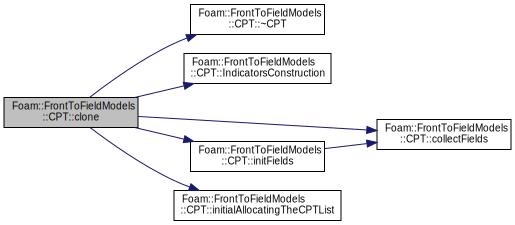
\includegraphics[width=350pt]{classFoam_1_1FrontToFieldModels_1_1CPT_a1ba03c46bac4bba07f9ee8185baff1e6_cgraph}
\end{center}
\end{figure}
\mbox{\Hypertarget{classFoam_1_1FrontToFieldModels_1_1CPT_a1ba03c46bac4bba07f9ee8185baff1e6}\label{classFoam_1_1FrontToFieldModels_1_1CPT_a1ba03c46bac4bba07f9ee8185baff1e6}} 
\index{Foam\+::\+Front\+To\+Field\+Models\+::\+C\+PT@{Foam\+::\+Front\+To\+Field\+Models\+::\+C\+PT}!clone@{clone}}
\index{clone@{clone}!Foam\+::\+Front\+To\+Field\+Models\+::\+C\+PT@{Foam\+::\+Front\+To\+Field\+Models\+::\+C\+PT}}
\subsubsection{\texorpdfstring{clone()}{clone()}\hspace{0.1cm}{\footnotesize\ttfamily [2/2]}}
{\footnotesize\ttfamily template$<$class Cloud\+Type$>$ \\
virtual auto\+Ptr$<$\hyperlink{classFoam_1_1FrontToFieldModel}{Front\+To\+Field\+Model}$<$Cloud\+Type$>$ $>$ \hyperlink{classFoam_1_1FrontToFieldModels_1_1CPT}{Foam\+::\+Front\+To\+Field\+Models\+::\+C\+PT}$<$ Cloud\+Type $>$\+::clone (\begin{DoxyParamCaption}{ }\end{DoxyParamCaption}) const\hspace{0.3cm}{\ttfamily [inline]}, {\ttfamily [virtual]}}



Implements \hyperlink{classFoam_1_1FrontToFieldModels_1_1BaseF2FModel_a28a0e5110316e77393efe30b9f243b08}{Foam\+::\+Front\+To\+Field\+Models\+::\+Base\+F2\+F\+Model$<$ Cloud\+Type $>$}.

Here is the call graph for this function\+:
\nopagebreak
\begin{figure}[H]
\begin{center}
\leavevmode
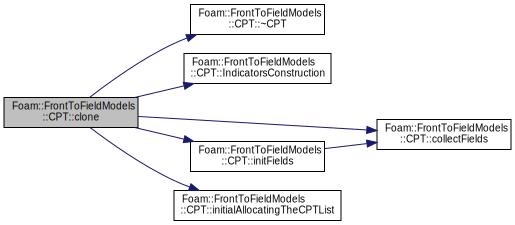
\includegraphics[width=350pt]{classFoam_1_1FrontToFieldModels_1_1CPT_a1ba03c46bac4bba07f9ee8185baff1e6_cgraph}
\end{center}
\end{figure}
\mbox{\Hypertarget{classFoam_1_1FrontToFieldModels_1_1CPT_a30ebffabafd2b102fd189269ffa3be2a}\label{classFoam_1_1FrontToFieldModels_1_1CPT_a30ebffabafd2b102fd189269ffa3be2a}} 
\index{Foam\+::\+Front\+To\+Field\+Models\+::\+C\+PT@{Foam\+::\+Front\+To\+Field\+Models\+::\+C\+PT}!collect\+Fields@{collect\+Fields}}
\index{collect\+Fields@{collect\+Fields}!Foam\+::\+Front\+To\+Field\+Models\+::\+C\+PT@{Foam\+::\+Front\+To\+Field\+Models\+::\+C\+PT}}
\subsubsection{\texorpdfstring{collect\+Fields()}{collectFields()}\hspace{0.1cm}{\footnotesize\ttfamily [1/2]}}
{\footnotesize\ttfamily template$<$class Cloud\+Type $>$ \\
void \hyperlink{classFoam_1_1FrontToFieldModels_1_1CPT}{Foam\+::\+Front\+To\+Field\+Models\+::\+C\+PT}$<$ Cloud\+Type $>$\+::collect\+Fields (\begin{DoxyParamCaption}\item[{label}]{cellI,  }\item[{label}]{b\+DI,  }\item[{scalar}]{w\+Bar,  }\item[{vector}]{el\+Area\+Vec }\end{DoxyParamCaption})\hspace{0.3cm}{\ttfamily [virtual]}}



Implements \hyperlink{classFoam_1_1FrontToFieldModels_1_1BaseF2FModel_a22b3c4bb9f2660656b958208684ac9f8}{Foam\+::\+Front\+To\+Field\+Models\+::\+Base\+F2\+F\+Model$<$ Cloud\+Type $>$}.

Here is the caller graph for this function\+:\nopagebreak
\begin{figure}[H]
\begin{center}
\leavevmode
\includegraphics[width=350pt]{classFoam_1_1FrontToFieldModels_1_1CPT_a30ebffabafd2b102fd189269ffa3be2a_icgraph}
\end{center}
\end{figure}
\mbox{\Hypertarget{classFoam_1_1FrontToFieldModels_1_1CPT_ab2567f9d6b26e90f31c50c73cf62d32b}\label{classFoam_1_1FrontToFieldModels_1_1CPT_ab2567f9d6b26e90f31c50c73cf62d32b}} 
\index{Foam\+::\+Front\+To\+Field\+Models\+::\+C\+PT@{Foam\+::\+Front\+To\+Field\+Models\+::\+C\+PT}!collect\+Fields@{collect\+Fields}}
\index{collect\+Fields@{collect\+Fields}!Foam\+::\+Front\+To\+Field\+Models\+::\+C\+PT@{Foam\+::\+Front\+To\+Field\+Models\+::\+C\+PT}}
\subsubsection{\texorpdfstring{collect\+Fields()}{collectFields()}\hspace{0.1cm}{\footnotesize\ttfamily [2/2]}}
{\footnotesize\ttfamily template$<$class Cloud\+Type$>$ \\
virtual void \hyperlink{classFoam_1_1FrontToFieldModels_1_1CPT}{Foam\+::\+Front\+To\+Field\+Models\+::\+C\+PT}$<$ Cloud\+Type $>$\+::collect\+Fields (\begin{DoxyParamCaption}\item[{label}]{cellI,  }\item[{label}]{b\+DI,  }\item[{scalar}]{w\+Bar,  }\item[{vector}]{el\+Area\+Vec }\end{DoxyParamCaption})\hspace{0.3cm}{\ttfamily [virtual]}}



Implements \hyperlink{classFoam_1_1FrontToFieldModels_1_1BaseF2FModel_a22b3c4bb9f2660656b958208684ac9f8}{Foam\+::\+Front\+To\+Field\+Models\+::\+Base\+F2\+F\+Model$<$ Cloud\+Type $>$}.

\mbox{\Hypertarget{classFoam_1_1FrontToFieldModels_1_1CPT_a3d1350ef9a447e3dbafa181f8195761c}\label{classFoam_1_1FrontToFieldModels_1_1CPT_a3d1350ef9a447e3dbafa181f8195761c}} 
\index{Foam\+::\+Front\+To\+Field\+Models\+::\+C\+PT@{Foam\+::\+Front\+To\+Field\+Models\+::\+C\+PT}!Indicators\+Construction@{Indicators\+Construction}}
\index{Indicators\+Construction@{Indicators\+Construction}!Foam\+::\+Front\+To\+Field\+Models\+::\+C\+PT@{Foam\+::\+Front\+To\+Field\+Models\+::\+C\+PT}}
\subsubsection{\texorpdfstring{Indicators\+Construction()}{IndicatorsConstruction()}\hspace{0.1cm}{\footnotesize\ttfamily [1/2]}}
{\footnotesize\ttfamily template$<$class Cloud\+Type$>$ \\
virtual void \hyperlink{classFoam_1_1FrontToFieldModels_1_1CPT}{Foam\+::\+Front\+To\+Field\+Models\+::\+C\+PT}$<$ Cloud\+Type $>$\+::Indicators\+Construction (\begin{DoxyParamCaption}{ }\end{DoxyParamCaption})\hspace{0.3cm}{\ttfamily [virtual]}}



Implements \hyperlink{classFoam_1_1FrontToFieldModels_1_1BaseF2FModel_a194c0c309124ae1cfcd5bf07b3d3528e}{Foam\+::\+Front\+To\+Field\+Models\+::\+Base\+F2\+F\+Model$<$ Cloud\+Type $>$}.

\mbox{\Hypertarget{classFoam_1_1FrontToFieldModels_1_1CPT_a8c38f2d1f3cad1e29d337ad43ca05309}\label{classFoam_1_1FrontToFieldModels_1_1CPT_a8c38f2d1f3cad1e29d337ad43ca05309}} 
\index{Foam\+::\+Front\+To\+Field\+Models\+::\+C\+PT@{Foam\+::\+Front\+To\+Field\+Models\+::\+C\+PT}!Indicators\+Construction@{Indicators\+Construction}}
\index{Indicators\+Construction@{Indicators\+Construction}!Foam\+::\+Front\+To\+Field\+Models\+::\+C\+PT@{Foam\+::\+Front\+To\+Field\+Models\+::\+C\+PT}}
\subsubsection{\texorpdfstring{Indicators\+Construction()}{IndicatorsConstruction()}\hspace{0.1cm}{\footnotesize\ttfamily [2/2]}}
{\footnotesize\ttfamily template$<$class Cloud\+Type $>$ \\
void \hyperlink{classFoam_1_1FrontToFieldModels_1_1CPT}{Foam\+::\+Front\+To\+Field\+Models\+::\+C\+PT}$<$ Cloud\+Type $>$\+::Indicators\+Construction (\begin{DoxyParamCaption}{ }\end{DoxyParamCaption})\hspace{0.3cm}{\ttfamily [virtual]}}



Implements \hyperlink{classFoam_1_1FrontToFieldModels_1_1BaseF2FModel_a194c0c309124ae1cfcd5bf07b3d3528e}{Foam\+::\+Front\+To\+Field\+Models\+::\+Base\+F2\+F\+Model$<$ Cloud\+Type $>$}.

Here is the caller graph for this function\+:\nopagebreak
\begin{figure}[H]
\begin{center}
\leavevmode
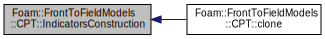
\includegraphics[width=350pt]{classFoam_1_1FrontToFieldModels_1_1CPT_a8c38f2d1f3cad1e29d337ad43ca05309_icgraph}
\end{center}
\end{figure}
\mbox{\Hypertarget{classFoam_1_1FrontToFieldModels_1_1CPT_a81f9b6cb7a4f16d31e87fbcff452800b}\label{classFoam_1_1FrontToFieldModels_1_1CPT_a81f9b6cb7a4f16d31e87fbcff452800b}} 
\index{Foam\+::\+Front\+To\+Field\+Models\+::\+C\+PT@{Foam\+::\+Front\+To\+Field\+Models\+::\+C\+PT}!init\+Fields@{init\+Fields}}
\index{init\+Fields@{init\+Fields}!Foam\+::\+Front\+To\+Field\+Models\+::\+C\+PT@{Foam\+::\+Front\+To\+Field\+Models\+::\+C\+PT}}
\subsubsection{\texorpdfstring{init\+Fields()}{initFields()}\hspace{0.1cm}{\footnotesize\ttfamily [1/2]}}
{\footnotesize\ttfamily template$<$class Cloud\+Type $>$ \\
void \hyperlink{classFoam_1_1FrontToFieldModels_1_1CPT}{Foam\+::\+Front\+To\+Field\+Models\+::\+C\+PT}$<$ Cloud\+Type $>$\+::init\+Fields (\begin{DoxyParamCaption}{ }\end{DoxyParamCaption})\hspace{0.3cm}{\ttfamily [virtual]}}



Implements \hyperlink{classFoam_1_1FrontToFieldModels_1_1BaseF2FModel_af404778ce26acab686dd1184da5749c5}{Foam\+::\+Front\+To\+Field\+Models\+::\+Base\+F2\+F\+Model$<$ Cloud\+Type $>$}.

Here is the call graph for this function\+:\nopagebreak
\begin{figure}[H]
\begin{center}
\leavevmode
\includegraphics[width=350pt]{classFoam_1_1FrontToFieldModels_1_1CPT_a81f9b6cb7a4f16d31e87fbcff452800b_cgraph}
\end{center}
\end{figure}
Here is the caller graph for this function\+:\nopagebreak
\begin{figure}[H]
\begin{center}
\leavevmode
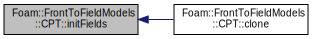
\includegraphics[width=350pt]{classFoam_1_1FrontToFieldModels_1_1CPT_a81f9b6cb7a4f16d31e87fbcff452800b_icgraph}
\end{center}
\end{figure}
\mbox{\Hypertarget{classFoam_1_1FrontToFieldModels_1_1CPT_a051e181306632a5cc5fde3fdb7094c9a}\label{classFoam_1_1FrontToFieldModels_1_1CPT_a051e181306632a5cc5fde3fdb7094c9a}} 
\index{Foam\+::\+Front\+To\+Field\+Models\+::\+C\+PT@{Foam\+::\+Front\+To\+Field\+Models\+::\+C\+PT}!init\+Fields@{init\+Fields}}
\index{init\+Fields@{init\+Fields}!Foam\+::\+Front\+To\+Field\+Models\+::\+C\+PT@{Foam\+::\+Front\+To\+Field\+Models\+::\+C\+PT}}
\subsubsection{\texorpdfstring{init\+Fields()}{initFields()}\hspace{0.1cm}{\footnotesize\ttfamily [2/2]}}
{\footnotesize\ttfamily template$<$class Cloud\+Type$>$ \\
virtual void \hyperlink{classFoam_1_1FrontToFieldModels_1_1CPT}{Foam\+::\+Front\+To\+Field\+Models\+::\+C\+PT}$<$ Cloud\+Type $>$\+::init\+Fields (\begin{DoxyParamCaption}{ }\end{DoxyParamCaption})\hspace{0.3cm}{\ttfamily [virtual]}}



Implements \hyperlink{classFoam_1_1FrontToFieldModels_1_1BaseF2FModel_af404778ce26acab686dd1184da5749c5}{Foam\+::\+Front\+To\+Field\+Models\+::\+Base\+F2\+F\+Model$<$ Cloud\+Type $>$}.

\mbox{\Hypertarget{classFoam_1_1FrontToFieldModels_1_1CPT_ad44422a69564bdcf0cd2ead0015d9226}\label{classFoam_1_1FrontToFieldModels_1_1CPT_ad44422a69564bdcf0cd2ead0015d9226}} 
\index{Foam\+::\+Front\+To\+Field\+Models\+::\+C\+PT@{Foam\+::\+Front\+To\+Field\+Models\+::\+C\+PT}!initial\+Allocating\+The\+C\+P\+T\+List@{initial\+Allocating\+The\+C\+P\+T\+List}}
\index{initial\+Allocating\+The\+C\+P\+T\+List@{initial\+Allocating\+The\+C\+P\+T\+List}!Foam\+::\+Front\+To\+Field\+Models\+::\+C\+PT@{Foam\+::\+Front\+To\+Field\+Models\+::\+C\+PT}}
\subsubsection{\texorpdfstring{initial\+Allocating\+The\+C\+P\+T\+List()}{initialAllocatingTheCPTList()}\hspace{0.1cm}{\footnotesize\ttfamily [1/2]}}
{\footnotesize\ttfamily template$<$class Cloud\+Type$>$ \\
void Front\+To\+Field\+Models\+::\+C\+P\+T\+::initial\+Allocating\+The\+C\+P\+T\+List (\begin{DoxyParamCaption}{ }\end{DoxyParamCaption})\hspace{0.3cm}{\ttfamily [inline]}}

\mbox{\Hypertarget{classFoam_1_1FrontToFieldModels_1_1CPT_a6a2bc39ec3cf7a842515a5661c9f4584}\label{classFoam_1_1FrontToFieldModels_1_1CPT_a6a2bc39ec3cf7a842515a5661c9f4584}} 
\index{Foam\+::\+Front\+To\+Field\+Models\+::\+C\+PT@{Foam\+::\+Front\+To\+Field\+Models\+::\+C\+PT}!initial\+Allocating\+The\+C\+P\+T\+List@{initial\+Allocating\+The\+C\+P\+T\+List}}
\index{initial\+Allocating\+The\+C\+P\+T\+List@{initial\+Allocating\+The\+C\+P\+T\+List}!Foam\+::\+Front\+To\+Field\+Models\+::\+C\+PT@{Foam\+::\+Front\+To\+Field\+Models\+::\+C\+PT}}
\subsubsection{\texorpdfstring{initial\+Allocating\+The\+C\+P\+T\+List()}{initialAllocatingTheCPTList()}\hspace{0.1cm}{\footnotesize\ttfamily [2/2]}}
{\footnotesize\ttfamily template$<$class Cloud\+Type$>$ \\
void \hyperlink{classFoam_1_1FrontToFieldModels_1_1CPT}{Foam\+::\+Front\+To\+Field\+Models\+::\+C\+PT}$<$ Cloud\+Type $>$\+::initial\+Allocating\+The\+C\+P\+T\+List (\begin{DoxyParamCaption}{ }\end{DoxyParamCaption})\hspace{0.3cm}{\ttfamily [inline]}}

Here is the caller graph for this function\+:\nopagebreak
\begin{figure}[H]
\begin{center}
\leavevmode
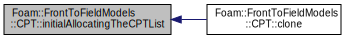
\includegraphics[width=350pt]{classFoam_1_1FrontToFieldModels_1_1CPT_a6a2bc39ec3cf7a842515a5661c9f4584_icgraph}
\end{center}
\end{figure}
\mbox{\Hypertarget{classFoam_1_1FrontToFieldModels_1_1CPT_a288cadbe2779addeaf65f4994bb8f465}\label{classFoam_1_1FrontToFieldModels_1_1CPT_a288cadbe2779addeaf65f4994bb8f465}} 
\index{Foam\+::\+Front\+To\+Field\+Models\+::\+C\+PT@{Foam\+::\+Front\+To\+Field\+Models\+::\+C\+PT}!Type\+Name@{Type\+Name}}
\index{Type\+Name@{Type\+Name}!Foam\+::\+Front\+To\+Field\+Models\+::\+C\+PT@{Foam\+::\+Front\+To\+Field\+Models\+::\+C\+PT}}
\subsubsection{\texorpdfstring{Type\+Name()}{TypeName()}\hspace{0.1cm}{\footnotesize\ttfamily [1/2]}}
{\footnotesize\ttfamily template$<$class Cloud\+Type$>$ \\
\hyperlink{classFoam_1_1FrontToFieldModels_1_1CPT}{Foam\+::\+Front\+To\+Field\+Models\+::\+C\+PT}$<$ Cloud\+Type $>$\+::Type\+Name (\begin{DoxyParamCaption}\item[{\char`\"{}cpt\char`\"{}}]{ }\end{DoxyParamCaption})}

\mbox{\Hypertarget{classFoam_1_1FrontToFieldModels_1_1CPT_a288cadbe2779addeaf65f4994bb8f465}\label{classFoam_1_1FrontToFieldModels_1_1CPT_a288cadbe2779addeaf65f4994bb8f465}} 
\index{Foam\+::\+Front\+To\+Field\+Models\+::\+C\+PT@{Foam\+::\+Front\+To\+Field\+Models\+::\+C\+PT}!Type\+Name@{Type\+Name}}
\index{Type\+Name@{Type\+Name}!Foam\+::\+Front\+To\+Field\+Models\+::\+C\+PT@{Foam\+::\+Front\+To\+Field\+Models\+::\+C\+PT}}
\subsubsection{\texorpdfstring{Type\+Name()}{TypeName()}\hspace{0.1cm}{\footnotesize\ttfamily [2/2]}}
{\footnotesize\ttfamily template$<$class Cloud\+Type$>$ \\
\hyperlink{classFoam_1_1FrontToFieldModels_1_1CPT}{Foam\+::\+Front\+To\+Field\+Models\+::\+C\+PT}$<$ Cloud\+Type $>$\+::Type\+Name (\begin{DoxyParamCaption}\item[{\char`\"{}cpt\char`\"{}}]{ }\end{DoxyParamCaption})}



\subsection{Member Data Documentation}
\mbox{\Hypertarget{classFoam_1_1FrontToFieldModels_1_1CPT_acc46ef6b49688a927bc95b8967b1099b}\label{classFoam_1_1FrontToFieldModels_1_1CPT_acc46ef6b49688a927bc95b8967b1099b}} 
\index{Foam\+::\+Front\+To\+Field\+Models\+::\+C\+PT@{Foam\+::\+Front\+To\+Field\+Models\+::\+C\+PT}!C\+P\+T\+List\+\_\+@{C\+P\+T\+List\+\_\+}}
\index{C\+P\+T\+List\+\_\+@{C\+P\+T\+List\+\_\+}!Foam\+::\+Front\+To\+Field\+Models\+::\+C\+PT@{Foam\+::\+Front\+To\+Field\+Models\+::\+C\+PT}}
\subsubsection{\texorpdfstring{C\+P\+T\+List\+\_\+}{CPTList\_}}
{\footnotesize\ttfamily template$<$class Cloud\+Type$>$ \\
List$<$ \hyperlink{classFoam_1_1FrontToFieldModels_1_1CPT_1_1CPTData}{C\+P\+T\+Data} $>$ \hyperlink{classFoam_1_1FrontToFieldModels_1_1CPT}{Foam\+::\+Front\+To\+Field\+Models\+::\+C\+PT}$<$ Cloud\+Type $>$\+::C\+P\+T\+List\+\_\+}



The documentation for this class was generated from the following files\+:\begin{DoxyCompactItemize}
\item 
ln\+Include/\hyperlink{lnInclude_2CPT_8H}{C\+P\+T.\+H}\item 
ln\+Include/\hyperlink{lnInclude_2CPT_8C}{C\+P\+T.\+C}\end{DoxyCompactItemize}

\hypertarget{classFoam_1_1FrontToFieldModels_1_1CPT_1_1CPTData}{}\section{Foam\+:\+:Front\+To\+Field\+Models\+:\+:C\+PT$<$ Cloud\+Type $>$\+:\+:C\+P\+T\+Data Class Reference}
\label{classFoam_1_1FrontToFieldModels_1_1CPT_1_1CPTData}\index{Foam\+::\+Front\+To\+Field\+Models\+::\+C\+P\+T$<$ Cloud\+Type $>$\+::\+C\+P\+T\+Data@{Foam\+::\+Front\+To\+Field\+Models\+::\+C\+P\+T$<$ Cloud\+Type $>$\+::\+C\+P\+T\+Data}}


{\ttfamily \#include $<$C\+P\+T.\+H$>$}



Collaboration diagram for Foam\+:\+:Front\+To\+Field\+Models\+:\+:C\+PT$<$ Cloud\+Type $>$\+:\+:C\+P\+T\+Data\+:\nopagebreak
\begin{figure}[H]
\begin{center}
\leavevmode
\includegraphics[width=235pt]{classFoam_1_1FrontToFieldModels_1_1CPT_1_1CPTData__coll__graph}
\end{center}
\end{figure}
\subsection*{Public Member Functions}
\begin{DoxyCompactItemize}
\item 
\hyperlink{classFoam_1_1FrontToFieldModels_1_1CPT_1_1CPTData_acd8172c7ace7c296e1b55b73fd4fadd6}{C\+P\+T\+Data} ()
\item 
\hyperlink{classFoam_1_1FrontToFieldModels_1_1CPT_1_1CPTData_acd8172c7ace7c296e1b55b73fd4fadd6}{C\+P\+T\+Data} ()
\end{DoxyCompactItemize}
\subsection*{Public Attributes}
\begin{DoxyCompactItemize}
\item 
List$<$ scalar $>$ \hyperlink{classFoam_1_1FrontToFieldModels_1_1CPT_1_1CPTData_a92bd872d7773810a23f529f5bb1f60b6}{induced\+Density}
\item 
List$<$ scalar $>$ \hyperlink{classFoam_1_1FrontToFieldModels_1_1CPT_1_1CPTData_a59bd1c9540de547b2bd246debdaebd0f}{induced\+Viscosity}
\end{DoxyCompactItemize}


\subsection{Constructor \& Destructor Documentation}
\mbox{\Hypertarget{classFoam_1_1FrontToFieldModels_1_1CPT_1_1CPTData_acd8172c7ace7c296e1b55b73fd4fadd6}\label{classFoam_1_1FrontToFieldModels_1_1CPT_1_1CPTData_acd8172c7ace7c296e1b55b73fd4fadd6}} 
\index{Foam\+::\+Front\+To\+Field\+Models\+::\+C\+P\+T\+::\+C\+P\+T\+Data@{Foam\+::\+Front\+To\+Field\+Models\+::\+C\+P\+T\+::\+C\+P\+T\+Data}!C\+P\+T\+Data@{C\+P\+T\+Data}}
\index{C\+P\+T\+Data@{C\+P\+T\+Data}!Foam\+::\+Front\+To\+Field\+Models\+::\+C\+P\+T\+::\+C\+P\+T\+Data@{Foam\+::\+Front\+To\+Field\+Models\+::\+C\+P\+T\+::\+C\+P\+T\+Data}}
\subsubsection{\texorpdfstring{C\+P\+T\+Data()}{CPTData()}\hspace{0.1cm}{\footnotesize\ttfamily [1/2]}}
{\footnotesize\ttfamily template$<$class Cloud\+Type$>$ \\
\hyperlink{classFoam_1_1FrontToFieldModels_1_1CPT}{Foam\+::\+Front\+To\+Field\+Models\+::\+C\+PT}$<$ Cloud\+Type $>$\+::C\+P\+T\+Data\+::\+C\+P\+T\+Data (\begin{DoxyParamCaption}{ }\end{DoxyParamCaption})\hspace{0.3cm}{\ttfamily [inline]}}

\mbox{\Hypertarget{classFoam_1_1FrontToFieldModels_1_1CPT_1_1CPTData_acd8172c7ace7c296e1b55b73fd4fadd6}\label{classFoam_1_1FrontToFieldModels_1_1CPT_1_1CPTData_acd8172c7ace7c296e1b55b73fd4fadd6}} 
\index{Foam\+::\+Front\+To\+Field\+Models\+::\+C\+P\+T\+::\+C\+P\+T\+Data@{Foam\+::\+Front\+To\+Field\+Models\+::\+C\+P\+T\+::\+C\+P\+T\+Data}!C\+P\+T\+Data@{C\+P\+T\+Data}}
\index{C\+P\+T\+Data@{C\+P\+T\+Data}!Foam\+::\+Front\+To\+Field\+Models\+::\+C\+P\+T\+::\+C\+P\+T\+Data@{Foam\+::\+Front\+To\+Field\+Models\+::\+C\+P\+T\+::\+C\+P\+T\+Data}}
\subsubsection{\texorpdfstring{C\+P\+T\+Data()}{CPTData()}\hspace{0.1cm}{\footnotesize\ttfamily [2/2]}}
{\footnotesize\ttfamily template$<$class Cloud\+Type$>$ \\
\hyperlink{classFoam_1_1FrontToFieldModels_1_1CPT}{Foam\+::\+Front\+To\+Field\+Models\+::\+C\+PT}$<$ Cloud\+Type $>$\+::C\+P\+T\+Data\+::\+C\+P\+T\+Data (\begin{DoxyParamCaption}{ }\end{DoxyParamCaption})\hspace{0.3cm}{\ttfamily [inline]}}

Here is the call graph for this function\+:\nopagebreak
\begin{figure}[H]
\begin{center}
\leavevmode
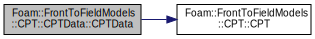
\includegraphics[width=350pt]{classFoam_1_1FrontToFieldModels_1_1CPT_1_1CPTData_acd8172c7ace7c296e1b55b73fd4fadd6_cgraph}
\end{center}
\end{figure}


\subsection{Member Data Documentation}
\mbox{\Hypertarget{classFoam_1_1FrontToFieldModels_1_1CPT_1_1CPTData_a92bd872d7773810a23f529f5bb1f60b6}\label{classFoam_1_1FrontToFieldModels_1_1CPT_1_1CPTData_a92bd872d7773810a23f529f5bb1f60b6}} 
\index{Foam\+::\+Front\+To\+Field\+Models\+::\+C\+P\+T\+::\+C\+P\+T\+Data@{Foam\+::\+Front\+To\+Field\+Models\+::\+C\+P\+T\+::\+C\+P\+T\+Data}!induced\+Density@{induced\+Density}}
\index{induced\+Density@{induced\+Density}!Foam\+::\+Front\+To\+Field\+Models\+::\+C\+P\+T\+::\+C\+P\+T\+Data@{Foam\+::\+Front\+To\+Field\+Models\+::\+C\+P\+T\+::\+C\+P\+T\+Data}}
\subsubsection{\texorpdfstring{induced\+Density}{inducedDensity}}
{\footnotesize\ttfamily template$<$class Cloud\+Type$>$ \\
List$<$ scalar $>$ \hyperlink{classFoam_1_1FrontToFieldModels_1_1CPT}{Foam\+::\+Front\+To\+Field\+Models\+::\+C\+PT}$<$ Cloud\+Type $>$\+::C\+P\+T\+Data\+::induced\+Density}

\mbox{\Hypertarget{classFoam_1_1FrontToFieldModels_1_1CPT_1_1CPTData_a59bd1c9540de547b2bd246debdaebd0f}\label{classFoam_1_1FrontToFieldModels_1_1CPT_1_1CPTData_a59bd1c9540de547b2bd246debdaebd0f}} 
\index{Foam\+::\+Front\+To\+Field\+Models\+::\+C\+P\+T\+::\+C\+P\+T\+Data@{Foam\+::\+Front\+To\+Field\+Models\+::\+C\+P\+T\+::\+C\+P\+T\+Data}!induced\+Viscosity@{induced\+Viscosity}}
\index{induced\+Viscosity@{induced\+Viscosity}!Foam\+::\+Front\+To\+Field\+Models\+::\+C\+P\+T\+::\+C\+P\+T\+Data@{Foam\+::\+Front\+To\+Field\+Models\+::\+C\+P\+T\+::\+C\+P\+T\+Data}}
\subsubsection{\texorpdfstring{induced\+Viscosity}{inducedViscosity}}
{\footnotesize\ttfamily template$<$class Cloud\+Type$>$ \\
List$<$ scalar $>$ \hyperlink{classFoam_1_1FrontToFieldModels_1_1CPT}{Foam\+::\+Front\+To\+Field\+Models\+::\+C\+PT}$<$ Cloud\+Type $>$\+::C\+P\+T\+Data\+::induced\+Viscosity}



The documentation for this class was generated from the following file\+:\begin{DoxyCompactItemize}
\item 
ln\+Include/\hyperlink{lnInclude_2CPT_8H}{C\+P\+T.\+H}\end{DoxyCompactItemize}

\hypertarget{classFoam_1_1SurfaceTensionModels_1_1DirectElementBased}{}\section{Foam\+:\+:Surface\+Tension\+Models\+:\+:Direct\+Element\+Based$<$ Cloud\+Type $>$ Class Template Reference}
\label{classFoam_1_1SurfaceTensionModels_1_1DirectElementBased}\index{Foam\+::\+Surface\+Tension\+Models\+::\+Direct\+Element\+Based$<$ Cloud\+Type $>$@{Foam\+::\+Surface\+Tension\+Models\+::\+Direct\+Element\+Based$<$ Cloud\+Type $>$}}


{\ttfamily \#include $<$Direct\+Element\+Based.\+H$>$}



Inheritance diagram for Foam\+:\+:Surface\+Tension\+Models\+:\+:Direct\+Element\+Based$<$ Cloud\+Type $>$\+:\nopagebreak
\begin{figure}[H]
\begin{center}
\leavevmode
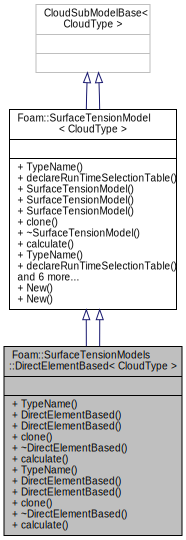
\includegraphics[height=550pt]{classFoam_1_1SurfaceTensionModels_1_1DirectElementBased__inherit__graph}
\end{center}
\end{figure}


Collaboration diagram for Foam\+:\+:Surface\+Tension\+Models\+:\+:Direct\+Element\+Based$<$ Cloud\+Type $>$\+:\nopagebreak
\begin{figure}[H]
\begin{center}
\leavevmode
\includegraphics[height=550pt]{classFoam_1_1SurfaceTensionModels_1_1DirectElementBased__coll__graph}
\end{center}
\end{figure}
\subsection*{Public Member Functions}
\begin{DoxyCompactItemize}
\item 
\hyperlink{classFoam_1_1SurfaceTensionModels_1_1DirectElementBased_a90abb05ec7462e2e317912c3b644924c}{Type\+Name} (\char`\"{}direct\+Element\+Based\char`\"{})
\item 
\hyperlink{classFoam_1_1SurfaceTensionModels_1_1DirectElementBased_a907db1967f98b8b4d8e068798c036bc3}{Direct\+Element\+Based} (const dictionary \&dict, Cloud\+Type \&owner)
\item 
\hyperlink{classFoam_1_1SurfaceTensionModels_1_1DirectElementBased_a988187a377c2d987417c0800af92ee8f}{Direct\+Element\+Based} (const \hyperlink{classFoam_1_1SurfaceTensionModels_1_1DirectElementBased}{Direct\+Element\+Based}$<$ Cloud\+Type $>$ \&cm)
\item 
virtual auto\+Ptr$<$ \hyperlink{classFoam_1_1SurfaceTensionModel}{Surface\+Tension\+Model}$<$ Cloud\+Type $>$ $>$ \hyperlink{classFoam_1_1SurfaceTensionModels_1_1DirectElementBased_a6b88fc625943a7e49a1d8fdfd676496e}{clone} () const
\item 
virtual \hyperlink{classFoam_1_1SurfaceTensionModels_1_1DirectElementBased_afe9b049df358d7b179df6b45e2960eba}{$\sim$\+Direct\+Element\+Based} ()
\item 
virtual void \hyperlink{classFoam_1_1SurfaceTensionModels_1_1DirectElementBased_acddfca0be38d2b652a7c188388997f48}{calculate} ()
\item 
\hyperlink{classFoam_1_1SurfaceTensionModels_1_1DirectElementBased_a90abb05ec7462e2e317912c3b644924c}{Type\+Name} (\char`\"{}direct\+Element\+Based\char`\"{})
\item 
\hyperlink{classFoam_1_1SurfaceTensionModels_1_1DirectElementBased_a907db1967f98b8b4d8e068798c036bc3}{Direct\+Element\+Based} (const dictionary \&dict, Cloud\+Type \&owner)
\item 
\hyperlink{classFoam_1_1SurfaceTensionModels_1_1DirectElementBased_a988187a377c2d987417c0800af92ee8f}{Direct\+Element\+Based} (const \hyperlink{classFoam_1_1SurfaceTensionModels_1_1DirectElementBased}{Direct\+Element\+Based}$<$ Cloud\+Type $>$ \&cm)
\item 
virtual auto\+Ptr$<$ \hyperlink{classFoam_1_1SurfaceTensionModel}{Surface\+Tension\+Model}$<$ Cloud\+Type $>$ $>$ \hyperlink{classFoam_1_1SurfaceTensionModels_1_1DirectElementBased_a6b88fc625943a7e49a1d8fdfd676496e}{clone} () const
\item 
virtual \hyperlink{classFoam_1_1SurfaceTensionModels_1_1DirectElementBased_ad0f49729fbfc64cf1a2784b2bcbe6350}{$\sim$\+Direct\+Element\+Based} ()
\item 
virtual void \hyperlink{classFoam_1_1SurfaceTensionModels_1_1DirectElementBased_a5fff46598e2d383978ffc826f8566a47}{calculate} ()
\end{DoxyCompactItemize}
\subsection*{Additional Inherited Members}


\subsection{Constructor \& Destructor Documentation}
\mbox{\Hypertarget{classFoam_1_1SurfaceTensionModels_1_1DirectElementBased_a907db1967f98b8b4d8e068798c036bc3}\label{classFoam_1_1SurfaceTensionModels_1_1DirectElementBased_a907db1967f98b8b4d8e068798c036bc3}} 
\index{Foam\+::\+Surface\+Tension\+Models\+::\+Direct\+Element\+Based@{Foam\+::\+Surface\+Tension\+Models\+::\+Direct\+Element\+Based}!Direct\+Element\+Based@{Direct\+Element\+Based}}
\index{Direct\+Element\+Based@{Direct\+Element\+Based}!Foam\+::\+Surface\+Tension\+Models\+::\+Direct\+Element\+Based@{Foam\+::\+Surface\+Tension\+Models\+::\+Direct\+Element\+Based}}
\subsubsection{\texorpdfstring{Direct\+Element\+Based()}{DirectElementBased()}\hspace{0.1cm}{\footnotesize\ttfamily [1/4]}}
{\footnotesize\ttfamily template$<$class Cloud\+Type $>$ \\
\hyperlink{classFoam_1_1SurfaceTensionModels_1_1DirectElementBased}{Foam\+::\+Surface\+Tension\+Models\+::\+Direct\+Element\+Based}$<$ Cloud\+Type $>$\+::\hyperlink{classFoam_1_1SurfaceTensionModels_1_1DirectElementBased}{Direct\+Element\+Based} (\begin{DoxyParamCaption}\item[{const dictionary \&}]{dict,  }\item[{Cloud\+Type \&}]{owner }\end{DoxyParamCaption})}

\mbox{\Hypertarget{classFoam_1_1SurfaceTensionModels_1_1DirectElementBased_a988187a377c2d987417c0800af92ee8f}\label{classFoam_1_1SurfaceTensionModels_1_1DirectElementBased_a988187a377c2d987417c0800af92ee8f}} 
\index{Foam\+::\+Surface\+Tension\+Models\+::\+Direct\+Element\+Based@{Foam\+::\+Surface\+Tension\+Models\+::\+Direct\+Element\+Based}!Direct\+Element\+Based@{Direct\+Element\+Based}}
\index{Direct\+Element\+Based@{Direct\+Element\+Based}!Foam\+::\+Surface\+Tension\+Models\+::\+Direct\+Element\+Based@{Foam\+::\+Surface\+Tension\+Models\+::\+Direct\+Element\+Based}}
\subsubsection{\texorpdfstring{Direct\+Element\+Based()}{DirectElementBased()}\hspace{0.1cm}{\footnotesize\ttfamily [2/4]}}
{\footnotesize\ttfamily template$<$class Cloud\+Type $>$ \\
\hyperlink{classFoam_1_1SurfaceTensionModels_1_1DirectElementBased}{Foam\+::\+Surface\+Tension\+Models\+::\+Direct\+Element\+Based}$<$ Cloud\+Type $>$\+::\hyperlink{classFoam_1_1SurfaceTensionModels_1_1DirectElementBased}{Direct\+Element\+Based} (\begin{DoxyParamCaption}\item[{const \hyperlink{classFoam_1_1SurfaceTensionModels_1_1DirectElementBased}{Direct\+Element\+Based}$<$ Cloud\+Type $>$ \&}]{cm }\end{DoxyParamCaption})}

\mbox{\Hypertarget{classFoam_1_1SurfaceTensionModels_1_1DirectElementBased_afe9b049df358d7b179df6b45e2960eba}\label{classFoam_1_1SurfaceTensionModels_1_1DirectElementBased_afe9b049df358d7b179df6b45e2960eba}} 
\index{Foam\+::\+Surface\+Tension\+Models\+::\+Direct\+Element\+Based@{Foam\+::\+Surface\+Tension\+Models\+::\+Direct\+Element\+Based}!````~Direct\+Element\+Based@{$\sim$\+Direct\+Element\+Based}}
\index{````~Direct\+Element\+Based@{$\sim$\+Direct\+Element\+Based}!Foam\+::\+Surface\+Tension\+Models\+::\+Direct\+Element\+Based@{Foam\+::\+Surface\+Tension\+Models\+::\+Direct\+Element\+Based}}
\subsubsection{\texorpdfstring{$\sim$\+Direct\+Element\+Based()}{~DirectElementBased()}\hspace{0.1cm}{\footnotesize\ttfamily [1/2]}}
{\footnotesize\ttfamily template$<$class Cloud\+Type $>$ \\
\hyperlink{classFoam_1_1SurfaceTensionModels_1_1DirectElementBased}{Foam\+::\+Surface\+Tension\+Models\+::\+Direct\+Element\+Based}$<$ Cloud\+Type $>$\+::$\sim$\hyperlink{classFoam_1_1SurfaceTensionModels_1_1DirectElementBased}{Direct\+Element\+Based} (\begin{DoxyParamCaption}{ }\end{DoxyParamCaption})\hspace{0.3cm}{\ttfamily [virtual]}}

Here is the caller graph for this function\+:\nopagebreak
\begin{figure}[H]
\begin{center}
\leavevmode
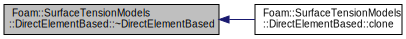
\includegraphics[width=350pt]{classFoam_1_1SurfaceTensionModels_1_1DirectElementBased_afe9b049df358d7b179df6b45e2960eba_icgraph}
\end{center}
\end{figure}
\mbox{\Hypertarget{classFoam_1_1SurfaceTensionModels_1_1DirectElementBased_a907db1967f98b8b4d8e068798c036bc3}\label{classFoam_1_1SurfaceTensionModels_1_1DirectElementBased_a907db1967f98b8b4d8e068798c036bc3}} 
\index{Foam\+::\+Surface\+Tension\+Models\+::\+Direct\+Element\+Based@{Foam\+::\+Surface\+Tension\+Models\+::\+Direct\+Element\+Based}!Direct\+Element\+Based@{Direct\+Element\+Based}}
\index{Direct\+Element\+Based@{Direct\+Element\+Based}!Foam\+::\+Surface\+Tension\+Models\+::\+Direct\+Element\+Based@{Foam\+::\+Surface\+Tension\+Models\+::\+Direct\+Element\+Based}}
\subsubsection{\texorpdfstring{Direct\+Element\+Based()}{DirectElementBased()}\hspace{0.1cm}{\footnotesize\ttfamily [3/4]}}
{\footnotesize\ttfamily template$<$class Cloud\+Type$>$ \\
\hyperlink{classFoam_1_1SurfaceTensionModels_1_1DirectElementBased}{Foam\+::\+Surface\+Tension\+Models\+::\+Direct\+Element\+Based}$<$ Cloud\+Type $>$\+::\hyperlink{classFoam_1_1SurfaceTensionModels_1_1DirectElementBased}{Direct\+Element\+Based} (\begin{DoxyParamCaption}\item[{const dictionary \&}]{dict,  }\item[{Cloud\+Type \&}]{owner }\end{DoxyParamCaption})}

\mbox{\Hypertarget{classFoam_1_1SurfaceTensionModels_1_1DirectElementBased_a988187a377c2d987417c0800af92ee8f}\label{classFoam_1_1SurfaceTensionModels_1_1DirectElementBased_a988187a377c2d987417c0800af92ee8f}} 
\index{Foam\+::\+Surface\+Tension\+Models\+::\+Direct\+Element\+Based@{Foam\+::\+Surface\+Tension\+Models\+::\+Direct\+Element\+Based}!Direct\+Element\+Based@{Direct\+Element\+Based}}
\index{Direct\+Element\+Based@{Direct\+Element\+Based}!Foam\+::\+Surface\+Tension\+Models\+::\+Direct\+Element\+Based@{Foam\+::\+Surface\+Tension\+Models\+::\+Direct\+Element\+Based}}
\subsubsection{\texorpdfstring{Direct\+Element\+Based()}{DirectElementBased()}\hspace{0.1cm}{\footnotesize\ttfamily [4/4]}}
{\footnotesize\ttfamily template$<$class Cloud\+Type$>$ \\
\hyperlink{classFoam_1_1SurfaceTensionModels_1_1DirectElementBased}{Foam\+::\+Surface\+Tension\+Models\+::\+Direct\+Element\+Based}$<$ Cloud\+Type $>$\+::\hyperlink{classFoam_1_1SurfaceTensionModels_1_1DirectElementBased}{Direct\+Element\+Based} (\begin{DoxyParamCaption}\item[{const \hyperlink{classFoam_1_1SurfaceTensionModels_1_1DirectElementBased}{Direct\+Element\+Based}$<$ Cloud\+Type $>$ \&}]{cm }\end{DoxyParamCaption})}

\mbox{\Hypertarget{classFoam_1_1SurfaceTensionModels_1_1DirectElementBased_ad0f49729fbfc64cf1a2784b2bcbe6350}\label{classFoam_1_1SurfaceTensionModels_1_1DirectElementBased_ad0f49729fbfc64cf1a2784b2bcbe6350}} 
\index{Foam\+::\+Surface\+Tension\+Models\+::\+Direct\+Element\+Based@{Foam\+::\+Surface\+Tension\+Models\+::\+Direct\+Element\+Based}!````~Direct\+Element\+Based@{$\sim$\+Direct\+Element\+Based}}
\index{````~Direct\+Element\+Based@{$\sim$\+Direct\+Element\+Based}!Foam\+::\+Surface\+Tension\+Models\+::\+Direct\+Element\+Based@{Foam\+::\+Surface\+Tension\+Models\+::\+Direct\+Element\+Based}}
\subsubsection{\texorpdfstring{$\sim$\+Direct\+Element\+Based()}{~DirectElementBased()}\hspace{0.1cm}{\footnotesize\ttfamily [2/2]}}
{\footnotesize\ttfamily template$<$class Cloud\+Type$>$ \\
virtual \hyperlink{classFoam_1_1SurfaceTensionModels_1_1DirectElementBased}{Foam\+::\+Surface\+Tension\+Models\+::\+Direct\+Element\+Based}$<$ Cloud\+Type $>$\+::$\sim$\hyperlink{classFoam_1_1SurfaceTensionModels_1_1DirectElementBased}{Direct\+Element\+Based} (\begin{DoxyParamCaption}{ }\end{DoxyParamCaption})\hspace{0.3cm}{\ttfamily [virtual]}}



\subsection{Member Function Documentation}
\mbox{\Hypertarget{classFoam_1_1SurfaceTensionModels_1_1DirectElementBased_acddfca0be38d2b652a7c188388997f48}\label{classFoam_1_1SurfaceTensionModels_1_1DirectElementBased_acddfca0be38d2b652a7c188388997f48}} 
\index{Foam\+::\+Surface\+Tension\+Models\+::\+Direct\+Element\+Based@{Foam\+::\+Surface\+Tension\+Models\+::\+Direct\+Element\+Based}!calculate@{calculate}}
\index{calculate@{calculate}!Foam\+::\+Surface\+Tension\+Models\+::\+Direct\+Element\+Based@{Foam\+::\+Surface\+Tension\+Models\+::\+Direct\+Element\+Based}}
\subsubsection{\texorpdfstring{calculate()}{calculate()}\hspace{0.1cm}{\footnotesize\ttfamily [1/2]}}
{\footnotesize\ttfamily template$<$class Cloud\+Type $>$ \\
void \hyperlink{classFoam_1_1SurfaceTensionModels_1_1DirectElementBased}{Foam\+::\+Surface\+Tension\+Models\+::\+Direct\+Element\+Based}$<$ Cloud\+Type $>$\+::calculate (\begin{DoxyParamCaption}{ }\end{DoxyParamCaption})\hspace{0.3cm}{\ttfamily [virtual]}}



Implements \hyperlink{classFoam_1_1SurfaceTensionModel_ae511f83b3ea32268b67cdb0690182f22}{Foam\+::\+Surface\+Tension\+Model$<$ Cloud\+Type $>$}.

Here is the caller graph for this function\+:\nopagebreak
\begin{figure}[H]
\begin{center}
\leavevmode
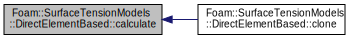
\includegraphics[width=350pt]{classFoam_1_1SurfaceTensionModels_1_1DirectElementBased_acddfca0be38d2b652a7c188388997f48_icgraph}
\end{center}
\end{figure}
\mbox{\Hypertarget{classFoam_1_1SurfaceTensionModels_1_1DirectElementBased_a5fff46598e2d383978ffc826f8566a47}\label{classFoam_1_1SurfaceTensionModels_1_1DirectElementBased_a5fff46598e2d383978ffc826f8566a47}} 
\index{Foam\+::\+Surface\+Tension\+Models\+::\+Direct\+Element\+Based@{Foam\+::\+Surface\+Tension\+Models\+::\+Direct\+Element\+Based}!calculate@{calculate}}
\index{calculate@{calculate}!Foam\+::\+Surface\+Tension\+Models\+::\+Direct\+Element\+Based@{Foam\+::\+Surface\+Tension\+Models\+::\+Direct\+Element\+Based}}
\subsubsection{\texorpdfstring{calculate()}{calculate()}\hspace{0.1cm}{\footnotesize\ttfamily [2/2]}}
{\footnotesize\ttfamily template$<$class Cloud\+Type$>$ \\
virtual void \hyperlink{classFoam_1_1SurfaceTensionModels_1_1DirectElementBased}{Foam\+::\+Surface\+Tension\+Models\+::\+Direct\+Element\+Based}$<$ Cloud\+Type $>$\+::calculate (\begin{DoxyParamCaption}{ }\end{DoxyParamCaption})\hspace{0.3cm}{\ttfamily [virtual]}}



Implements \hyperlink{classFoam_1_1SurfaceTensionModel_ae511f83b3ea32268b67cdb0690182f22}{Foam\+::\+Surface\+Tension\+Model$<$ Cloud\+Type $>$}.

\mbox{\Hypertarget{classFoam_1_1SurfaceTensionModels_1_1DirectElementBased_a6b88fc625943a7e49a1d8fdfd676496e}\label{classFoam_1_1SurfaceTensionModels_1_1DirectElementBased_a6b88fc625943a7e49a1d8fdfd676496e}} 
\index{Foam\+::\+Surface\+Tension\+Models\+::\+Direct\+Element\+Based@{Foam\+::\+Surface\+Tension\+Models\+::\+Direct\+Element\+Based}!clone@{clone}}
\index{clone@{clone}!Foam\+::\+Surface\+Tension\+Models\+::\+Direct\+Element\+Based@{Foam\+::\+Surface\+Tension\+Models\+::\+Direct\+Element\+Based}}
\subsubsection{\texorpdfstring{clone()}{clone()}\hspace{0.1cm}{\footnotesize\ttfamily [1/2]}}
{\footnotesize\ttfamily template$<$class Cloud\+Type$>$ \\
virtual auto\+Ptr$<$\hyperlink{classFoam_1_1SurfaceTensionModel}{Surface\+Tension\+Model}$<$Cloud\+Type$>$ $>$ \hyperlink{classFoam_1_1SurfaceTensionModels_1_1DirectElementBased}{Foam\+::\+Surface\+Tension\+Models\+::\+Direct\+Element\+Based}$<$ Cloud\+Type $>$\+::clone (\begin{DoxyParamCaption}{ }\end{DoxyParamCaption}) const\hspace{0.3cm}{\ttfamily [inline]}, {\ttfamily [virtual]}}



Implements \hyperlink{classFoam_1_1SurfaceTensionModel_a8f9800b94267ba07be098824ef33dde6}{Foam\+::\+Surface\+Tension\+Model$<$ Cloud\+Type $>$}.

Here is the call graph for this function\+:
\nopagebreak
\begin{figure}[H]
\begin{center}
\leavevmode
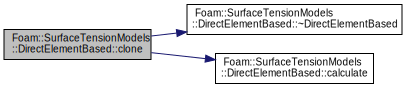
\includegraphics[width=350pt]{classFoam_1_1SurfaceTensionModels_1_1DirectElementBased_a6b88fc625943a7e49a1d8fdfd676496e_cgraph}
\end{center}
\end{figure}
\mbox{\Hypertarget{classFoam_1_1SurfaceTensionModels_1_1DirectElementBased_a6b88fc625943a7e49a1d8fdfd676496e}\label{classFoam_1_1SurfaceTensionModels_1_1DirectElementBased_a6b88fc625943a7e49a1d8fdfd676496e}} 
\index{Foam\+::\+Surface\+Tension\+Models\+::\+Direct\+Element\+Based@{Foam\+::\+Surface\+Tension\+Models\+::\+Direct\+Element\+Based}!clone@{clone}}
\index{clone@{clone}!Foam\+::\+Surface\+Tension\+Models\+::\+Direct\+Element\+Based@{Foam\+::\+Surface\+Tension\+Models\+::\+Direct\+Element\+Based}}
\subsubsection{\texorpdfstring{clone()}{clone()}\hspace{0.1cm}{\footnotesize\ttfamily [2/2]}}
{\footnotesize\ttfamily template$<$class Cloud\+Type$>$ \\
virtual auto\+Ptr$<$\hyperlink{classFoam_1_1SurfaceTensionModel}{Surface\+Tension\+Model}$<$Cloud\+Type$>$ $>$ \hyperlink{classFoam_1_1SurfaceTensionModels_1_1DirectElementBased}{Foam\+::\+Surface\+Tension\+Models\+::\+Direct\+Element\+Based}$<$ Cloud\+Type $>$\+::clone (\begin{DoxyParamCaption}{ }\end{DoxyParamCaption}) const\hspace{0.3cm}{\ttfamily [inline]}, {\ttfamily [virtual]}}



Implements \hyperlink{classFoam_1_1SurfaceTensionModel_a8f9800b94267ba07be098824ef33dde6}{Foam\+::\+Surface\+Tension\+Model$<$ Cloud\+Type $>$}.

Here is the call graph for this function\+:
\nopagebreak
\begin{figure}[H]
\begin{center}
\leavevmode
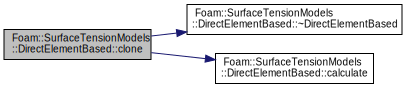
\includegraphics[width=350pt]{classFoam_1_1SurfaceTensionModels_1_1DirectElementBased_a6b88fc625943a7e49a1d8fdfd676496e_cgraph}
\end{center}
\end{figure}
\mbox{\Hypertarget{classFoam_1_1SurfaceTensionModels_1_1DirectElementBased_a90abb05ec7462e2e317912c3b644924c}\label{classFoam_1_1SurfaceTensionModels_1_1DirectElementBased_a90abb05ec7462e2e317912c3b644924c}} 
\index{Foam\+::\+Surface\+Tension\+Models\+::\+Direct\+Element\+Based@{Foam\+::\+Surface\+Tension\+Models\+::\+Direct\+Element\+Based}!Type\+Name@{Type\+Name}}
\index{Type\+Name@{Type\+Name}!Foam\+::\+Surface\+Tension\+Models\+::\+Direct\+Element\+Based@{Foam\+::\+Surface\+Tension\+Models\+::\+Direct\+Element\+Based}}
\subsubsection{\texorpdfstring{Type\+Name()}{TypeName()}\hspace{0.1cm}{\footnotesize\ttfamily [1/2]}}
{\footnotesize\ttfamily template$<$class Cloud\+Type$>$ \\
\hyperlink{classFoam_1_1SurfaceTensionModels_1_1DirectElementBased}{Foam\+::\+Surface\+Tension\+Models\+::\+Direct\+Element\+Based}$<$ Cloud\+Type $>$\+::Type\+Name (\begin{DoxyParamCaption}\item[{\char`\"{}direct\+Element\+Based\char`\"{}}]{ }\end{DoxyParamCaption})}

\mbox{\Hypertarget{classFoam_1_1SurfaceTensionModels_1_1DirectElementBased_a90abb05ec7462e2e317912c3b644924c}\label{classFoam_1_1SurfaceTensionModels_1_1DirectElementBased_a90abb05ec7462e2e317912c3b644924c}} 
\index{Foam\+::\+Surface\+Tension\+Models\+::\+Direct\+Element\+Based@{Foam\+::\+Surface\+Tension\+Models\+::\+Direct\+Element\+Based}!Type\+Name@{Type\+Name}}
\index{Type\+Name@{Type\+Name}!Foam\+::\+Surface\+Tension\+Models\+::\+Direct\+Element\+Based@{Foam\+::\+Surface\+Tension\+Models\+::\+Direct\+Element\+Based}}
\subsubsection{\texorpdfstring{Type\+Name()}{TypeName()}\hspace{0.1cm}{\footnotesize\ttfamily [2/2]}}
{\footnotesize\ttfamily template$<$class Cloud\+Type$>$ \\
\hyperlink{classFoam_1_1SurfaceTensionModels_1_1DirectElementBased}{Foam\+::\+Surface\+Tension\+Models\+::\+Direct\+Element\+Based}$<$ Cloud\+Type $>$\+::Type\+Name (\begin{DoxyParamCaption}\item[{\char`\"{}direct\+Element\+Based\char`\"{}}]{ }\end{DoxyParamCaption})}



The documentation for this class was generated from the following files\+:\begin{DoxyCompactItemize}
\item 
ln\+Include/\hyperlink{lnInclude_2DirectElementBased_8H}{Direct\+Element\+Based.\+H}\item 
ln\+Include/\hyperlink{lnInclude_2DirectElementBased_8C}{Direct\+Element\+Based.\+C}\end{DoxyCompactItemize}

\hypertarget{classFoam_1_1elementInfo}{}\section{Foam\+:\+:element\+Info Class Reference}
\label{classFoam_1_1elementInfo}\index{Foam\+::element\+Info@{Foam\+::element\+Info}}


{\ttfamily \#include $<$bubble\+Data.\+H$>$}



Collaboration diagram for Foam\+:\+:element\+Info\+:\nopagebreak
\begin{figure}[H]
\begin{center}
\leavevmode
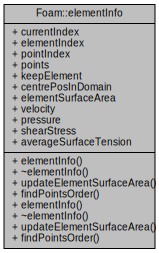
\includegraphics[width=231pt]{classFoam_1_1elementInfo__coll__graph}
\end{center}
\end{figure}
\subsection*{Public Member Functions}
\begin{DoxyCompactItemize}
\item 
\hyperlink{classFoam_1_1elementInfo_ab77651a347108969dff0ec1ddd2bbf89}{element\+Info} ()
\item 
virtual \hyperlink{classFoam_1_1elementInfo_a41639c761c6b7960e101d3ad900033a0}{$\sim$element\+Info} ()
\item 
void \hyperlink{classFoam_1_1elementInfo_a63daef83c9da37fb88f88ca578814eac}{update\+Element\+Surface\+Area} ()
\item 
void \hyperlink{classFoam_1_1elementInfo_a3318a932982b91d66075a89a2a860212}{find\+Points\+Order} (label f, label \&c\+NI, label \&c\+N\+II, label \&c\+N\+I\+II)
\item 
\hyperlink{classFoam_1_1elementInfo_ab77651a347108969dff0ec1ddd2bbf89}{element\+Info} ()
\item 
virtual \hyperlink{classFoam_1_1elementInfo_a41639c761c6b7960e101d3ad900033a0}{$\sim$element\+Info} ()
\item 
void \hyperlink{classFoam_1_1elementInfo_a63daef83c9da37fb88f88ca578814eac}{update\+Element\+Surface\+Area} ()
\item 
void \hyperlink{classFoam_1_1elementInfo_a3318a932982b91d66075a89a2a860212}{find\+Points\+Order} (label f, label \&c\+NI, label \&c\+N\+II, label \&c\+N\+I\+II)
\end{DoxyCompactItemize}
\subsection*{Public Attributes}
\begin{DoxyCompactItemize}
\item 
label \hyperlink{classFoam_1_1elementInfo_aef593bfaa849d634113aabb84736b4dd}{current\+Index}
\item 
label\+List \hyperlink{classFoam_1_1elementInfo_a0ea88c7e78906b98fb3d3c16ee7b324c}{element\+Index}
\item 
label\+List \hyperlink{classFoam_1_1elementInfo_a2f38fd4f14fc665753510c14bbf4cd2c}{point\+Index}
\item 
List$<$ point $>$ \hyperlink{classFoam_1_1elementInfo_ad77d73064ea98612a4edea1c7402529c}{points}
\item 
bool \hyperlink{classFoam_1_1elementInfo_adaffb567e41575d101cf7ebd9c3ba505}{keep\+Element}
\item 
vector \hyperlink{classFoam_1_1elementInfo_af93110fb4239a8967b512922428755ee}{centre\+Pos\+In\+Domain}
\item 
vector \hyperlink{classFoam_1_1elementInfo_a476a077a4247d3416f07ee4da5f10de5}{element\+Surface\+Area}
\item 
vector \hyperlink{classFoam_1_1elementInfo_a798b081e45f43145afcd43ff930f3e46}{velocity}
\item 
scalar \hyperlink{classFoam_1_1elementInfo_ad52f731cde16c3bae60b69a21df1501f}{pressure}
\item 
symm\+Tensor \hyperlink{classFoam_1_1elementInfo_ae8d40db9632c902f5419df4a0e5a0d4b}{shear\+Stress}
\item 
vector \hyperlink{classFoam_1_1elementInfo_a35df6da224928e44580ba822a9724ce9}{average\+Surface\+Tension}
\end{DoxyCompactItemize}


\subsection{Constructor \& Destructor Documentation}
\mbox{\Hypertarget{classFoam_1_1elementInfo_ab77651a347108969dff0ec1ddd2bbf89}\label{classFoam_1_1elementInfo_ab77651a347108969dff0ec1ddd2bbf89}} 
\index{Foam\+::element\+Info@{Foam\+::element\+Info}!element\+Info@{element\+Info}}
\index{element\+Info@{element\+Info}!Foam\+::element\+Info@{Foam\+::element\+Info}}
\subsubsection{\texorpdfstring{element\+Info()}{elementInfo()}\hspace{0.1cm}{\footnotesize\ttfamily [1/2]}}
{\footnotesize\ttfamily Foam\+::element\+Info\+::element\+Info (\begin{DoxyParamCaption}{ }\end{DoxyParamCaption})\hspace{0.3cm}{\ttfamily [inline]}}

\mbox{\Hypertarget{classFoam_1_1elementInfo_a41639c761c6b7960e101d3ad900033a0}\label{classFoam_1_1elementInfo_a41639c761c6b7960e101d3ad900033a0}} 
\index{Foam\+::element\+Info@{Foam\+::element\+Info}!````~element\+Info@{$\sim$element\+Info}}
\index{````~element\+Info@{$\sim$element\+Info}!Foam\+::element\+Info@{Foam\+::element\+Info}}
\subsubsection{\texorpdfstring{$\sim$element\+Info()}{~elementInfo()}\hspace{0.1cm}{\footnotesize\ttfamily [1/2]}}
{\footnotesize\ttfamily virtual Foam\+::element\+Info\+::$\sim$element\+Info (\begin{DoxyParamCaption}{ }\end{DoxyParamCaption})\hspace{0.3cm}{\ttfamily [inline]}, {\ttfamily [virtual]}}

\mbox{\Hypertarget{classFoam_1_1elementInfo_ab77651a347108969dff0ec1ddd2bbf89}\label{classFoam_1_1elementInfo_ab77651a347108969dff0ec1ddd2bbf89}} 
\index{Foam\+::element\+Info@{Foam\+::element\+Info}!element\+Info@{element\+Info}}
\index{element\+Info@{element\+Info}!Foam\+::element\+Info@{Foam\+::element\+Info}}
\subsubsection{\texorpdfstring{element\+Info()}{elementInfo()}\hspace{0.1cm}{\footnotesize\ttfamily [2/2]}}
{\footnotesize\ttfamily Foam\+::element\+Info\+::element\+Info (\begin{DoxyParamCaption}{ }\end{DoxyParamCaption})\hspace{0.3cm}{\ttfamily [inline]}}

\mbox{\Hypertarget{classFoam_1_1elementInfo_a41639c761c6b7960e101d3ad900033a0}\label{classFoam_1_1elementInfo_a41639c761c6b7960e101d3ad900033a0}} 
\index{Foam\+::element\+Info@{Foam\+::element\+Info}!````~element\+Info@{$\sim$element\+Info}}
\index{````~element\+Info@{$\sim$element\+Info}!Foam\+::element\+Info@{Foam\+::element\+Info}}
\subsubsection{\texorpdfstring{$\sim$element\+Info()}{~elementInfo()}\hspace{0.1cm}{\footnotesize\ttfamily [2/2]}}
{\footnotesize\ttfamily virtual Foam\+::element\+Info\+::$\sim$element\+Info (\begin{DoxyParamCaption}{ }\end{DoxyParamCaption})\hspace{0.3cm}{\ttfamily [inline]}, {\ttfamily [virtual]}}



\subsection{Member Function Documentation}
\mbox{\Hypertarget{classFoam_1_1elementInfo_a3318a932982b91d66075a89a2a860212}\label{classFoam_1_1elementInfo_a3318a932982b91d66075a89a2a860212}} 
\index{Foam\+::element\+Info@{Foam\+::element\+Info}!find\+Points\+Order@{find\+Points\+Order}}
\index{find\+Points\+Order@{find\+Points\+Order}!Foam\+::element\+Info@{Foam\+::element\+Info}}
\subsubsection{\texorpdfstring{find\+Points\+Order()}{findPointsOrder()}\hspace{0.1cm}{\footnotesize\ttfamily [1/2]}}
{\footnotesize\ttfamily void Foam\+::element\+Info\+::find\+Points\+Order (\begin{DoxyParamCaption}\item[{label}]{f,  }\item[{label \&}]{c\+NI,  }\item[{label \&}]{c\+N\+II,  }\item[{label \&}]{c\+N\+I\+II }\end{DoxyParamCaption})\hspace{0.3cm}{\ttfamily [inline]}}

Here is the caller graph for this function\+:\nopagebreak
\begin{figure}[H]
\begin{center}
\leavevmode
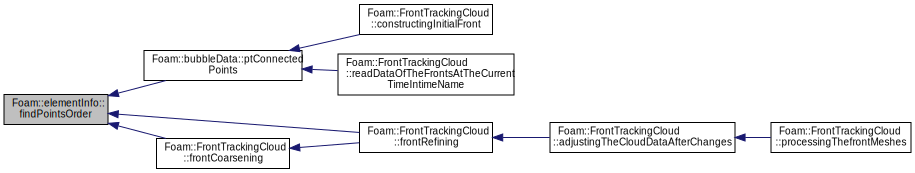
\includegraphics[width=350pt]{classFoam_1_1elementInfo_a3318a932982b91d66075a89a2a860212_icgraph}
\end{center}
\end{figure}
\mbox{\Hypertarget{classFoam_1_1elementInfo_a3318a932982b91d66075a89a2a860212}\label{classFoam_1_1elementInfo_a3318a932982b91d66075a89a2a860212}} 
\index{Foam\+::element\+Info@{Foam\+::element\+Info}!find\+Points\+Order@{find\+Points\+Order}}
\index{find\+Points\+Order@{find\+Points\+Order}!Foam\+::element\+Info@{Foam\+::element\+Info}}
\subsubsection{\texorpdfstring{find\+Points\+Order()}{findPointsOrder()}\hspace{0.1cm}{\footnotesize\ttfamily [2/2]}}
{\footnotesize\ttfamily void Foam\+::element\+Info\+::find\+Points\+Order (\begin{DoxyParamCaption}\item[{label}]{f,  }\item[{label \&}]{c\+NI,  }\item[{label \&}]{c\+N\+II,  }\item[{label \&}]{c\+N\+I\+II }\end{DoxyParamCaption})\hspace{0.3cm}{\ttfamily [inline]}}

\mbox{\Hypertarget{classFoam_1_1elementInfo_a63daef83c9da37fb88f88ca578814eac}\label{classFoam_1_1elementInfo_a63daef83c9da37fb88f88ca578814eac}} 
\index{Foam\+::element\+Info@{Foam\+::element\+Info}!update\+Element\+Surface\+Area@{update\+Element\+Surface\+Area}}
\index{update\+Element\+Surface\+Area@{update\+Element\+Surface\+Area}!Foam\+::element\+Info@{Foam\+::element\+Info}}
\subsubsection{\texorpdfstring{update\+Element\+Surface\+Area()}{updateElementSurfaceArea()}\hspace{0.1cm}{\footnotesize\ttfamily [1/2]}}
{\footnotesize\ttfamily void Foam\+::element\+Info\+::update\+Element\+Surface\+Area (\begin{DoxyParamCaption}{ }\end{DoxyParamCaption})\hspace{0.3cm}{\ttfamily [inline]}}

\mbox{\Hypertarget{classFoam_1_1elementInfo_a63daef83c9da37fb88f88ca578814eac}\label{classFoam_1_1elementInfo_a63daef83c9da37fb88f88ca578814eac}} 
\index{Foam\+::element\+Info@{Foam\+::element\+Info}!update\+Element\+Surface\+Area@{update\+Element\+Surface\+Area}}
\index{update\+Element\+Surface\+Area@{update\+Element\+Surface\+Area}!Foam\+::element\+Info@{Foam\+::element\+Info}}
\subsubsection{\texorpdfstring{update\+Element\+Surface\+Area()}{updateElementSurfaceArea()}\hspace{0.1cm}{\footnotesize\ttfamily [2/2]}}
{\footnotesize\ttfamily void Foam\+::element\+Info\+::update\+Element\+Surface\+Area (\begin{DoxyParamCaption}{ }\end{DoxyParamCaption})\hspace{0.3cm}{\ttfamily [inline]}}

Here is the caller graph for this function\+:\nopagebreak
\begin{figure}[H]
\begin{center}
\leavevmode
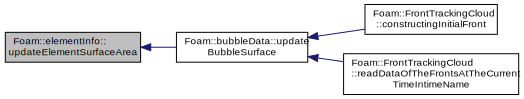
\includegraphics[width=350pt]{classFoam_1_1elementInfo_a63daef83c9da37fb88f88ca578814eac_icgraph}
\end{center}
\end{figure}


\subsection{Member Data Documentation}
\mbox{\Hypertarget{classFoam_1_1elementInfo_a35df6da224928e44580ba822a9724ce9}\label{classFoam_1_1elementInfo_a35df6da224928e44580ba822a9724ce9}} 
\index{Foam\+::element\+Info@{Foam\+::element\+Info}!average\+Surface\+Tension@{average\+Surface\+Tension}}
\index{average\+Surface\+Tension@{average\+Surface\+Tension}!Foam\+::element\+Info@{Foam\+::element\+Info}}
\subsubsection{\texorpdfstring{average\+Surface\+Tension}{averageSurfaceTension}}
{\footnotesize\ttfamily vector Foam\+::element\+Info\+::average\+Surface\+Tension}

\mbox{\Hypertarget{classFoam_1_1elementInfo_af93110fb4239a8967b512922428755ee}\label{classFoam_1_1elementInfo_af93110fb4239a8967b512922428755ee}} 
\index{Foam\+::element\+Info@{Foam\+::element\+Info}!centre\+Pos\+In\+Domain@{centre\+Pos\+In\+Domain}}
\index{centre\+Pos\+In\+Domain@{centre\+Pos\+In\+Domain}!Foam\+::element\+Info@{Foam\+::element\+Info}}
\subsubsection{\texorpdfstring{centre\+Pos\+In\+Domain}{centrePosInDomain}}
{\footnotesize\ttfamily vector Foam\+::element\+Info\+::centre\+Pos\+In\+Domain}

\mbox{\Hypertarget{classFoam_1_1elementInfo_aef593bfaa849d634113aabb84736b4dd}\label{classFoam_1_1elementInfo_aef593bfaa849d634113aabb84736b4dd}} 
\index{Foam\+::element\+Info@{Foam\+::element\+Info}!current\+Index@{current\+Index}}
\index{current\+Index@{current\+Index}!Foam\+::element\+Info@{Foam\+::element\+Info}}
\subsubsection{\texorpdfstring{current\+Index}{currentIndex}}
{\footnotesize\ttfamily label Foam\+::element\+Info\+::current\+Index}

\mbox{\Hypertarget{classFoam_1_1elementInfo_a0ea88c7e78906b98fb3d3c16ee7b324c}\label{classFoam_1_1elementInfo_a0ea88c7e78906b98fb3d3c16ee7b324c}} 
\index{Foam\+::element\+Info@{Foam\+::element\+Info}!element\+Index@{element\+Index}}
\index{element\+Index@{element\+Index}!Foam\+::element\+Info@{Foam\+::element\+Info}}
\subsubsection{\texorpdfstring{element\+Index}{elementIndex}}
{\footnotesize\ttfamily label\+List Foam\+::element\+Info\+::element\+Index}

\mbox{\Hypertarget{classFoam_1_1elementInfo_a476a077a4247d3416f07ee4da5f10de5}\label{classFoam_1_1elementInfo_a476a077a4247d3416f07ee4da5f10de5}} 
\index{Foam\+::element\+Info@{Foam\+::element\+Info}!element\+Surface\+Area@{element\+Surface\+Area}}
\index{element\+Surface\+Area@{element\+Surface\+Area}!Foam\+::element\+Info@{Foam\+::element\+Info}}
\subsubsection{\texorpdfstring{element\+Surface\+Area}{elementSurfaceArea}}
{\footnotesize\ttfamily vector Foam\+::element\+Info\+::element\+Surface\+Area}

\mbox{\Hypertarget{classFoam_1_1elementInfo_adaffb567e41575d101cf7ebd9c3ba505}\label{classFoam_1_1elementInfo_adaffb567e41575d101cf7ebd9c3ba505}} 
\index{Foam\+::element\+Info@{Foam\+::element\+Info}!keep\+Element@{keep\+Element}}
\index{keep\+Element@{keep\+Element}!Foam\+::element\+Info@{Foam\+::element\+Info}}
\subsubsection{\texorpdfstring{keep\+Element}{keepElement}}
{\footnotesize\ttfamily bool Foam\+::element\+Info\+::keep\+Element}

\mbox{\Hypertarget{classFoam_1_1elementInfo_a2f38fd4f14fc665753510c14bbf4cd2c}\label{classFoam_1_1elementInfo_a2f38fd4f14fc665753510c14bbf4cd2c}} 
\index{Foam\+::element\+Info@{Foam\+::element\+Info}!point\+Index@{point\+Index}}
\index{point\+Index@{point\+Index}!Foam\+::element\+Info@{Foam\+::element\+Info}}
\subsubsection{\texorpdfstring{point\+Index}{pointIndex}}
{\footnotesize\ttfamily label\+List Foam\+::element\+Info\+::point\+Index}

\mbox{\Hypertarget{classFoam_1_1elementInfo_ad77d73064ea98612a4edea1c7402529c}\label{classFoam_1_1elementInfo_ad77d73064ea98612a4edea1c7402529c}} 
\index{Foam\+::element\+Info@{Foam\+::element\+Info}!points@{points}}
\index{points@{points}!Foam\+::element\+Info@{Foam\+::element\+Info}}
\subsubsection{\texorpdfstring{points}{points}}
{\footnotesize\ttfamily List$<$ point $>$ Foam\+::element\+Info\+::points}

\mbox{\Hypertarget{classFoam_1_1elementInfo_ad52f731cde16c3bae60b69a21df1501f}\label{classFoam_1_1elementInfo_ad52f731cde16c3bae60b69a21df1501f}} 
\index{Foam\+::element\+Info@{Foam\+::element\+Info}!pressure@{pressure}}
\index{pressure@{pressure}!Foam\+::element\+Info@{Foam\+::element\+Info}}
\subsubsection{\texorpdfstring{pressure}{pressure}}
{\footnotesize\ttfamily scalar Foam\+::element\+Info\+::pressure}

\mbox{\Hypertarget{classFoam_1_1elementInfo_ae8d40db9632c902f5419df4a0e5a0d4b}\label{classFoam_1_1elementInfo_ae8d40db9632c902f5419df4a0e5a0d4b}} 
\index{Foam\+::element\+Info@{Foam\+::element\+Info}!shear\+Stress@{shear\+Stress}}
\index{shear\+Stress@{shear\+Stress}!Foam\+::element\+Info@{Foam\+::element\+Info}}
\subsubsection{\texorpdfstring{shear\+Stress}{shearStress}}
{\footnotesize\ttfamily symm\+Tensor Foam\+::element\+Info\+::shear\+Stress}

\mbox{\Hypertarget{classFoam_1_1elementInfo_a798b081e45f43145afcd43ff930f3e46}\label{classFoam_1_1elementInfo_a798b081e45f43145afcd43ff930f3e46}} 
\index{Foam\+::element\+Info@{Foam\+::element\+Info}!velocity@{velocity}}
\index{velocity@{velocity}!Foam\+::element\+Info@{Foam\+::element\+Info}}
\subsubsection{\texorpdfstring{velocity}{velocity}}
{\footnotesize\ttfamily vector Foam\+::element\+Info\+::velocity}



The documentation for this class was generated from the following files\+:\begin{DoxyCompactItemize}
\item 
clouds/\+Templates/\+Front\+Tracking\+Cloud/bubble\+Data/\hyperlink{clouds_2Templates_2FrontTrackingCloud_2bubbleData_2bubbleData_8H}{bubble\+Data.\+H}\item 
clouds/\+Templates/\+Front\+Tracking\+Cloud/bubble\+Data/\hyperlink{clouds_2Templates_2FrontTrackingCloud_2bubbleData_2bubbleDataI_8H}{bubble\+Data\+I.\+H}\end{DoxyCompactItemize}

\hypertarget{classFoam_1_1FrontToFieldModel}{}\section{Foam\+:\+:Front\+To\+Field\+Model$<$ Cloud\+Type $>$ Class Template Reference}
\label{classFoam_1_1FrontToFieldModel}\index{Foam\+::\+Front\+To\+Field\+Model$<$ Cloud\+Type $>$@{Foam\+::\+Front\+To\+Field\+Model$<$ Cloud\+Type $>$}}


{\ttfamily \#include $<$Front\+Tracking\+Cloud.\+H$>$}



Inheritance diagram for Foam\+:\+:Front\+To\+Field\+Model$<$ Cloud\+Type $>$\+:\nopagebreak
\begin{figure}[H]
\begin{center}
\leavevmode
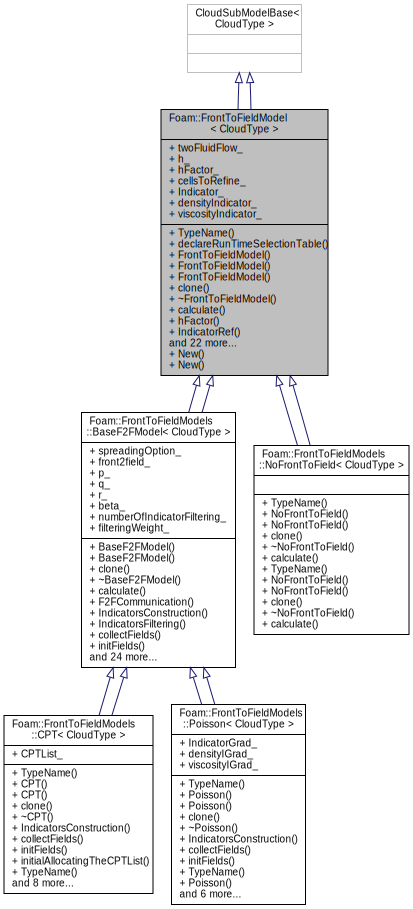
\includegraphics[height=550pt]{classFoam_1_1FrontToFieldModel__inherit__graph}
\end{center}
\end{figure}


Collaboration diagram for Foam\+:\+:Front\+To\+Field\+Model$<$ Cloud\+Type $>$\+:\nopagebreak
\begin{figure}[H]
\begin{center}
\leavevmode
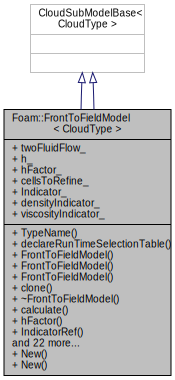
\includegraphics[width=247pt]{classFoam_1_1FrontToFieldModel__coll__graph}
\end{center}
\end{figure}
\subsection*{Public Member Functions}
\begin{DoxyCompactItemize}
\item 
\hyperlink{classFoam_1_1FrontToFieldModel_a6e113da5c0c612fe1313cffc439e44e9}{Type\+Name} (\char`\"{}front\+To\+Field\+Model\char`\"{})
\item 
\hyperlink{classFoam_1_1FrontToFieldModel_a9c10014640a00a66fd4c2683d511807e}{declare\+Run\+Time\+Selection\+Table} (auto\+Ptr, \hyperlink{classFoam_1_1FrontToFieldModel}{Front\+To\+Field\+Model}, dictionary,(const dictionary \&dict, Cloud\+Type \&owner),(dict, owner))
\item 
\hyperlink{classFoam_1_1FrontToFieldModel_a01d81526dcbb6ebcd6e6426bf7133b0b}{Front\+To\+Field\+Model} (Cloud\+Type \&owner)
\item 
\hyperlink{classFoam_1_1FrontToFieldModel_abb2f9f2dafb8b7abc44ddb676bf31ae6}{Front\+To\+Field\+Model} (const dictionary \&dict, Cloud\+Type \&owner, const word \&type)
\item 
\hyperlink{classFoam_1_1FrontToFieldModel_ac7f1606fac5eab3a1bcbc08468f365bd}{Front\+To\+Field\+Model} (const \hyperlink{classFoam_1_1FrontToFieldModel}{Front\+To\+Field\+Model}$<$ Cloud\+Type $>$ \&cm)
\item 
virtual auto\+Ptr$<$ \hyperlink{classFoam_1_1FrontToFieldModel}{Front\+To\+Field\+Model}$<$ Cloud\+Type $>$ $>$ \hyperlink{classFoam_1_1FrontToFieldModel_a0c13ce2692d43dece9d9e51f6c0c5fd6}{clone} () const =0
\item 
virtual \hyperlink{classFoam_1_1FrontToFieldModel_aa5e52b77046856d2d6d557ee3bee28e7}{$\sim$\+Front\+To\+Field\+Model} ()
\item 
virtual void \hyperlink{classFoam_1_1FrontToFieldModel_a88ce933bcfddfcb36401aba9c0776ae5}{calculate} ()=0
\item 
scalar \hyperlink{classFoam_1_1FrontToFieldModel_a1172056c000443e082f3356e9a1717a2}{h\+Factor} () const
\item 
vol\+Scalar\+Field \& \hyperlink{classFoam_1_1FrontToFieldModel_aa68185706596a628eefee2a870b4c6f3}{Indicator\+Ref} ()
\item 
tmp$<$ vol\+Scalar\+Field $>$ \hyperlink{classFoam_1_1FrontToFieldModel_a8225df17b4139b26c110870451b96de9}{Indicator} () const
\item 
vol\+Scalar\+Field \& \hyperlink{classFoam_1_1FrontToFieldModel_a977bc1d757adc68b17dbe985a5bdefdc}{density\+Indicator\+Ref} ()
\item 
tmp$<$ vol\+Scalar\+Field $>$ \hyperlink{classFoam_1_1FrontToFieldModel_a6425150d02e7babd4f65504f30c699ba}{density\+Indicator} () const
\item 
vol\+Scalar\+Field \& \hyperlink{classFoam_1_1FrontToFieldModel_a36a55af8f324d11462adfacaf082b75b}{viscosity\+Indicator\+Ref} ()
\item 
tmp$<$ vol\+Scalar\+Field $>$ \hyperlink{classFoam_1_1FrontToFieldModel_acd7d5c4007bd82eec12e23b6e7c0e6a4}{viscosity\+Indicator} () const
\item 
bool \hyperlink{classFoam_1_1FrontToFieldModel_a7a5035a704385de5435e9668c29c3d89}{two\+Fluid\+Flow} () const
\item 
\hyperlink{classFoam_1_1FrontToFieldModel_a6e113da5c0c612fe1313cffc439e44e9}{Type\+Name} (\char`\"{}front\+To\+Field\+Model\char`\"{})
\item 
\hyperlink{classFoam_1_1FrontToFieldModel_a9c10014640a00a66fd4c2683d511807e}{declare\+Run\+Time\+Selection\+Table} (auto\+Ptr, \hyperlink{classFoam_1_1FrontToFieldModel}{Front\+To\+Field\+Model}, dictionary,(const dictionary \&dict, Cloud\+Type \&owner),(dict, owner))
\item 
\hyperlink{classFoam_1_1FrontToFieldModel_a01d81526dcbb6ebcd6e6426bf7133b0b}{Front\+To\+Field\+Model} (Cloud\+Type \&owner)
\item 
\hyperlink{classFoam_1_1FrontToFieldModel_abb2f9f2dafb8b7abc44ddb676bf31ae6}{Front\+To\+Field\+Model} (const dictionary \&dict, Cloud\+Type \&owner, const word \&type)
\item 
\hyperlink{classFoam_1_1FrontToFieldModel_ac7f1606fac5eab3a1bcbc08468f365bd}{Front\+To\+Field\+Model} (const \hyperlink{classFoam_1_1FrontToFieldModel}{Front\+To\+Field\+Model}$<$ Cloud\+Type $>$ \&cm)
\item 
virtual auto\+Ptr$<$ \hyperlink{classFoam_1_1FrontToFieldModel}{Front\+To\+Field\+Model}$<$ Cloud\+Type $>$ $>$ \hyperlink{classFoam_1_1FrontToFieldModel_a0c13ce2692d43dece9d9e51f6c0c5fd6}{clone} () const =0
\item 
virtual \hyperlink{classFoam_1_1FrontToFieldModel_a6a7a461032065a07562611c83ab9a869}{$\sim$\+Front\+To\+Field\+Model} ()
\item 
virtual void \hyperlink{classFoam_1_1FrontToFieldModel_a88ce933bcfddfcb36401aba9c0776ae5}{calculate} ()=0
\item 
scalar \hyperlink{classFoam_1_1FrontToFieldModel_a1f99cd00a8322735361ed653ba20a541}{h\+Factor} () const
\item 
vol\+Scalar\+Field \& \hyperlink{classFoam_1_1FrontToFieldModel_a44bef45020f0a232108fbc2856413f1f}{Indicator\+Ref} ()
\item 
tmp$<$ vol\+Scalar\+Field $>$ \hyperlink{classFoam_1_1FrontToFieldModel_a6b91d473e08d4efce2e85f2eb149c87a}{Indicator} () const
\item 
vol\+Scalar\+Field \& \hyperlink{classFoam_1_1FrontToFieldModel_a5fcad8b6197d09e8cc0542c69c5b6b47}{density\+Indicator\+Ref} ()
\item 
tmp$<$ vol\+Scalar\+Field $>$ \hyperlink{classFoam_1_1FrontToFieldModel_af5875747df6bfd82ca29742926d8701d}{density\+Indicator} () const
\item 
vol\+Scalar\+Field \& \hyperlink{classFoam_1_1FrontToFieldModel_a473af3afa64c2a730b7c6a6c067708e8}{viscosity\+Indicator\+Ref} ()
\item 
tmp$<$ vol\+Scalar\+Field $>$ \hyperlink{classFoam_1_1FrontToFieldModel_aab2ed845099ce21bb0c3ab7ac0ac35c5}{viscosity\+Indicator} () const
\item 
bool \hyperlink{classFoam_1_1FrontToFieldModel_a7a5035a704385de5435e9668c29c3d89}{two\+Fluid\+Flow} () const
\end{DoxyCompactItemize}
\subsection*{Static Public Member Functions}
\begin{DoxyCompactItemize}
\item 
static auto\+Ptr$<$ \hyperlink{classFoam_1_1FrontToFieldModel}{Front\+To\+Field\+Model}$<$ Cloud\+Type $>$ $>$ \hyperlink{classFoam_1_1FrontToFieldModel_a8d2ede4c3699e6e7b24c7491723d576e}{New} (const dictionary \&dict, Cloud\+Type \&owner)
\item 
static auto\+Ptr$<$ \hyperlink{classFoam_1_1FrontToFieldModel}{Front\+To\+Field\+Model}$<$ Cloud\+Type $>$ $>$ \hyperlink{classFoam_1_1FrontToFieldModel_a7d5806a3fe473966bedb5d5815a03035}{New} (const dictionary \&dict, Cloud\+Type \&owner)
\end{DoxyCompactItemize}
\subsection*{Public Attributes}
\begin{DoxyCompactItemize}
\item 
bool \hyperlink{classFoam_1_1FrontToFieldModel_ad04fa93b89f90606f8f0f0111e29aef7}{two\+Fluid\+Flow\+\_\+}
\item 
scalar \hyperlink{classFoam_1_1FrontToFieldModel_a2eca985c837b4173dae0ab002b512c91}{h\+\_\+}
\item 
scalar \hyperlink{classFoam_1_1FrontToFieldModel_a775b7bec736f2ca57e1d03dcd6b7c873}{h\+Factor\+\_\+}
\item 
vol\+Scalar\+Field \hyperlink{classFoam_1_1FrontToFieldModel_af547073005a760654aa30b6e0fe4d41c}{cells\+To\+Refine\+\_\+}
\item 
auto\+Ptr$<$ vol\+Scalar\+Field $>$ \hyperlink{classFoam_1_1FrontToFieldModel_a95395337010439fe57e0ecc9ca2bb23a}{Indicator\+\_\+}
\item 
auto\+Ptr$<$ vol\+Scalar\+Field $>$ \hyperlink{classFoam_1_1FrontToFieldModel_a401f7fb4cf5ca62b7a333f9fa8dd89d7}{density\+Indicator\+\_\+}
\item 
auto\+Ptr$<$ vol\+Scalar\+Field $>$ \hyperlink{classFoam_1_1FrontToFieldModel_ace19a4b367734365c6e4367def23a06e}{viscosity\+Indicator\+\_\+}
\end{DoxyCompactItemize}


\subsection{Constructor \& Destructor Documentation}
\mbox{\Hypertarget{classFoam_1_1FrontToFieldModel_a01d81526dcbb6ebcd6e6426bf7133b0b}\label{classFoam_1_1FrontToFieldModel_a01d81526dcbb6ebcd6e6426bf7133b0b}} 
\index{Foam\+::\+Front\+To\+Field\+Model@{Foam\+::\+Front\+To\+Field\+Model}!Front\+To\+Field\+Model@{Front\+To\+Field\+Model}}
\index{Front\+To\+Field\+Model@{Front\+To\+Field\+Model}!Foam\+::\+Front\+To\+Field\+Model@{Foam\+::\+Front\+To\+Field\+Model}}
\subsubsection{\texorpdfstring{Front\+To\+Field\+Model()}{FrontToFieldModel()}\hspace{0.1cm}{\footnotesize\ttfamily [1/6]}}
{\footnotesize\ttfamily template$<$class Cloud\+Type $>$ \\
\hyperlink{classFoam_1_1FrontToFieldModel}{Foam\+::\+Front\+To\+Field\+Model}$<$ Cloud\+Type $>$\+::\hyperlink{classFoam_1_1FrontToFieldModel}{Front\+To\+Field\+Model} (\begin{DoxyParamCaption}\item[{Cloud\+Type \&}]{owner }\end{DoxyParamCaption})}

Here is the caller graph for this function\+:\nopagebreak
\begin{figure}[H]
\begin{center}
\leavevmode
\includegraphics[width=350pt]{classFoam_1_1FrontToFieldModel_a01d81526dcbb6ebcd6e6426bf7133b0b_icgraph}
\end{center}
\end{figure}
\mbox{\Hypertarget{classFoam_1_1FrontToFieldModel_abb2f9f2dafb8b7abc44ddb676bf31ae6}\label{classFoam_1_1FrontToFieldModel_abb2f9f2dafb8b7abc44ddb676bf31ae6}} 
\index{Foam\+::\+Front\+To\+Field\+Model@{Foam\+::\+Front\+To\+Field\+Model}!Front\+To\+Field\+Model@{Front\+To\+Field\+Model}}
\index{Front\+To\+Field\+Model@{Front\+To\+Field\+Model}!Foam\+::\+Front\+To\+Field\+Model@{Foam\+::\+Front\+To\+Field\+Model}}
\subsubsection{\texorpdfstring{Front\+To\+Field\+Model()}{FrontToFieldModel()}\hspace{0.1cm}{\footnotesize\ttfamily [2/6]}}
{\footnotesize\ttfamily template$<$class Cloud\+Type $>$ \\
\hyperlink{classFoam_1_1FrontToFieldModel}{Foam\+::\+Front\+To\+Field\+Model}$<$ Cloud\+Type $>$\+::\hyperlink{classFoam_1_1FrontToFieldModel}{Front\+To\+Field\+Model} (\begin{DoxyParamCaption}\item[{const dictionary \&}]{dict,  }\item[{Cloud\+Type \&}]{owner,  }\item[{const word \&}]{type }\end{DoxyParamCaption})}

Here is the call graph for this function\+:\nopagebreak
\begin{figure}[H]
\begin{center}
\leavevmode
\includegraphics[width=350pt]{classFoam_1_1FrontToFieldModel_abb2f9f2dafb8b7abc44ddb676bf31ae6_cgraph}
\end{center}
\end{figure}
\mbox{\Hypertarget{classFoam_1_1FrontToFieldModel_ac7f1606fac5eab3a1bcbc08468f365bd}\label{classFoam_1_1FrontToFieldModel_ac7f1606fac5eab3a1bcbc08468f365bd}} 
\index{Foam\+::\+Front\+To\+Field\+Model@{Foam\+::\+Front\+To\+Field\+Model}!Front\+To\+Field\+Model@{Front\+To\+Field\+Model}}
\index{Front\+To\+Field\+Model@{Front\+To\+Field\+Model}!Foam\+::\+Front\+To\+Field\+Model@{Foam\+::\+Front\+To\+Field\+Model}}
\subsubsection{\texorpdfstring{Front\+To\+Field\+Model()}{FrontToFieldModel()}\hspace{0.1cm}{\footnotesize\ttfamily [3/6]}}
{\footnotesize\ttfamily template$<$class Cloud\+Type $>$ \\
\hyperlink{classFoam_1_1FrontToFieldModel}{Foam\+::\+Front\+To\+Field\+Model}$<$ Cloud\+Type $>$\+::\hyperlink{classFoam_1_1FrontToFieldModel}{Front\+To\+Field\+Model} (\begin{DoxyParamCaption}\item[{const \hyperlink{classFoam_1_1FrontToFieldModel}{Front\+To\+Field\+Model}$<$ Cloud\+Type $>$ \&}]{cm }\end{DoxyParamCaption})}

\mbox{\Hypertarget{classFoam_1_1FrontToFieldModel_aa5e52b77046856d2d6d557ee3bee28e7}\label{classFoam_1_1FrontToFieldModel_aa5e52b77046856d2d6d557ee3bee28e7}} 
\index{Foam\+::\+Front\+To\+Field\+Model@{Foam\+::\+Front\+To\+Field\+Model}!````~Front\+To\+Field\+Model@{$\sim$\+Front\+To\+Field\+Model}}
\index{````~Front\+To\+Field\+Model@{$\sim$\+Front\+To\+Field\+Model}!Foam\+::\+Front\+To\+Field\+Model@{Foam\+::\+Front\+To\+Field\+Model}}
\subsubsection{\texorpdfstring{$\sim$\+Front\+To\+Field\+Model()}{~FrontToFieldModel()}\hspace{0.1cm}{\footnotesize\ttfamily [1/2]}}
{\footnotesize\ttfamily template$<$class Cloud\+Type $>$ \\
\hyperlink{classFoam_1_1FrontToFieldModel}{Foam\+::\+Front\+To\+Field\+Model}$<$ Cloud\+Type $>$\+::$\sim$\hyperlink{classFoam_1_1FrontToFieldModel}{Front\+To\+Field\+Model} (\begin{DoxyParamCaption}{ }\end{DoxyParamCaption})\hspace{0.3cm}{\ttfamily [virtual]}}

Here is the call graph for this function\+:\nopagebreak
\begin{figure}[H]
\begin{center}
\leavevmode
\includegraphics[width=350pt]{classFoam_1_1FrontToFieldModel_aa5e52b77046856d2d6d557ee3bee28e7_cgraph}
\end{center}
\end{figure}
\mbox{\Hypertarget{classFoam_1_1FrontToFieldModel_a01d81526dcbb6ebcd6e6426bf7133b0b}\label{classFoam_1_1FrontToFieldModel_a01d81526dcbb6ebcd6e6426bf7133b0b}} 
\index{Foam\+::\+Front\+To\+Field\+Model@{Foam\+::\+Front\+To\+Field\+Model}!Front\+To\+Field\+Model@{Front\+To\+Field\+Model}}
\index{Front\+To\+Field\+Model@{Front\+To\+Field\+Model}!Foam\+::\+Front\+To\+Field\+Model@{Foam\+::\+Front\+To\+Field\+Model}}
\subsubsection{\texorpdfstring{Front\+To\+Field\+Model()}{FrontToFieldModel()}\hspace{0.1cm}{\footnotesize\ttfamily [4/6]}}
{\footnotesize\ttfamily template$<$class Cloud\+Type$>$ \\
\hyperlink{classFoam_1_1FrontToFieldModel}{Foam\+::\+Front\+To\+Field\+Model}$<$ Cloud\+Type $>$\+::\hyperlink{classFoam_1_1FrontToFieldModel}{Front\+To\+Field\+Model} (\begin{DoxyParamCaption}\item[{Cloud\+Type \&}]{owner }\end{DoxyParamCaption})}

\mbox{\Hypertarget{classFoam_1_1FrontToFieldModel_abb2f9f2dafb8b7abc44ddb676bf31ae6}\label{classFoam_1_1FrontToFieldModel_abb2f9f2dafb8b7abc44ddb676bf31ae6}} 
\index{Foam\+::\+Front\+To\+Field\+Model@{Foam\+::\+Front\+To\+Field\+Model}!Front\+To\+Field\+Model@{Front\+To\+Field\+Model}}
\index{Front\+To\+Field\+Model@{Front\+To\+Field\+Model}!Foam\+::\+Front\+To\+Field\+Model@{Foam\+::\+Front\+To\+Field\+Model}}
\subsubsection{\texorpdfstring{Front\+To\+Field\+Model()}{FrontToFieldModel()}\hspace{0.1cm}{\footnotesize\ttfamily [5/6]}}
{\footnotesize\ttfamily template$<$class Cloud\+Type$>$ \\
\hyperlink{classFoam_1_1FrontToFieldModel}{Foam\+::\+Front\+To\+Field\+Model}$<$ Cloud\+Type $>$\+::\hyperlink{classFoam_1_1FrontToFieldModel}{Front\+To\+Field\+Model} (\begin{DoxyParamCaption}\item[{const dictionary \&}]{dict,  }\item[{Cloud\+Type \&}]{owner,  }\item[{const word \&}]{type }\end{DoxyParamCaption})}

\mbox{\Hypertarget{classFoam_1_1FrontToFieldModel_ac7f1606fac5eab3a1bcbc08468f365bd}\label{classFoam_1_1FrontToFieldModel_ac7f1606fac5eab3a1bcbc08468f365bd}} 
\index{Foam\+::\+Front\+To\+Field\+Model@{Foam\+::\+Front\+To\+Field\+Model}!Front\+To\+Field\+Model@{Front\+To\+Field\+Model}}
\index{Front\+To\+Field\+Model@{Front\+To\+Field\+Model}!Foam\+::\+Front\+To\+Field\+Model@{Foam\+::\+Front\+To\+Field\+Model}}
\subsubsection{\texorpdfstring{Front\+To\+Field\+Model()}{FrontToFieldModel()}\hspace{0.1cm}{\footnotesize\ttfamily [6/6]}}
{\footnotesize\ttfamily template$<$class Cloud\+Type$>$ \\
\hyperlink{classFoam_1_1FrontToFieldModel}{Foam\+::\+Front\+To\+Field\+Model}$<$ Cloud\+Type $>$\+::\hyperlink{classFoam_1_1FrontToFieldModel}{Front\+To\+Field\+Model} (\begin{DoxyParamCaption}\item[{const \hyperlink{classFoam_1_1FrontToFieldModel}{Front\+To\+Field\+Model}$<$ Cloud\+Type $>$ \&}]{cm }\end{DoxyParamCaption})}

\mbox{\Hypertarget{classFoam_1_1FrontToFieldModel_a6a7a461032065a07562611c83ab9a869}\label{classFoam_1_1FrontToFieldModel_a6a7a461032065a07562611c83ab9a869}} 
\index{Foam\+::\+Front\+To\+Field\+Model@{Foam\+::\+Front\+To\+Field\+Model}!````~Front\+To\+Field\+Model@{$\sim$\+Front\+To\+Field\+Model}}
\index{````~Front\+To\+Field\+Model@{$\sim$\+Front\+To\+Field\+Model}!Foam\+::\+Front\+To\+Field\+Model@{Foam\+::\+Front\+To\+Field\+Model}}
\subsubsection{\texorpdfstring{$\sim$\+Front\+To\+Field\+Model()}{~FrontToFieldModel()}\hspace{0.1cm}{\footnotesize\ttfamily [2/2]}}
{\footnotesize\ttfamily template$<$class Cloud\+Type$>$ \\
virtual \hyperlink{classFoam_1_1FrontToFieldModel}{Foam\+::\+Front\+To\+Field\+Model}$<$ Cloud\+Type $>$\+::$\sim$\hyperlink{classFoam_1_1FrontToFieldModel}{Front\+To\+Field\+Model} (\begin{DoxyParamCaption}{ }\end{DoxyParamCaption})\hspace{0.3cm}{\ttfamily [virtual]}}



\subsection{Member Function Documentation}
\mbox{\Hypertarget{classFoam_1_1FrontToFieldModel_a88ce933bcfddfcb36401aba9c0776ae5}\label{classFoam_1_1FrontToFieldModel_a88ce933bcfddfcb36401aba9c0776ae5}} 
\index{Foam\+::\+Front\+To\+Field\+Model@{Foam\+::\+Front\+To\+Field\+Model}!calculate@{calculate}}
\index{calculate@{calculate}!Foam\+::\+Front\+To\+Field\+Model@{Foam\+::\+Front\+To\+Field\+Model}}
\subsubsection{\texorpdfstring{calculate()}{calculate()}\hspace{0.1cm}{\footnotesize\ttfamily [1/2]}}
{\footnotesize\ttfamily template$<$class Cloud\+Type$>$ \\
virtual void \hyperlink{classFoam_1_1FrontToFieldModel}{Foam\+::\+Front\+To\+Field\+Model}$<$ Cloud\+Type $>$\+::calculate (\begin{DoxyParamCaption}{ }\end{DoxyParamCaption})\hspace{0.3cm}{\ttfamily [pure virtual]}}



Implemented in \hyperlink{classFoam_1_1FrontToFieldModels_1_1BaseF2FModel_a1fd66572a83b6ec47ac9c2fb86064f19}{Foam\+::\+Front\+To\+Field\+Models\+::\+Base\+F2\+F\+Model$<$ Cloud\+Type $>$}, \hyperlink{classFoam_1_1FrontToFieldModels_1_1BaseF2FModel_a9417a2284bfa038e22a927d5c8e7d54b}{Foam\+::\+Front\+To\+Field\+Models\+::\+Base\+F2\+F\+Model$<$ Cloud\+Type $>$}, \hyperlink{classFoam_1_1FrontToFieldModels_1_1NoFrontToField_a02cb174d3171c5d71c38d1718f4bed23}{Foam\+::\+Front\+To\+Field\+Models\+::\+No\+Front\+To\+Field$<$ Cloud\+Type $>$}, and \hyperlink{classFoam_1_1FrontToFieldModels_1_1NoFrontToField_a168d2df0f3829473637252d412c3a1d3}{Foam\+::\+Front\+To\+Field\+Models\+::\+No\+Front\+To\+Field$<$ Cloud\+Type $>$}.

\mbox{\Hypertarget{classFoam_1_1FrontToFieldModel_a88ce933bcfddfcb36401aba9c0776ae5}\label{classFoam_1_1FrontToFieldModel_a88ce933bcfddfcb36401aba9c0776ae5}} 
\index{Foam\+::\+Front\+To\+Field\+Model@{Foam\+::\+Front\+To\+Field\+Model}!calculate@{calculate}}
\index{calculate@{calculate}!Foam\+::\+Front\+To\+Field\+Model@{Foam\+::\+Front\+To\+Field\+Model}}
\subsubsection{\texorpdfstring{calculate()}{calculate()}\hspace{0.1cm}{\footnotesize\ttfamily [2/2]}}
{\footnotesize\ttfamily template$<$class Cloud\+Type$>$ \\
virtual void \hyperlink{classFoam_1_1FrontToFieldModel}{Foam\+::\+Front\+To\+Field\+Model}$<$ Cloud\+Type $>$\+::calculate (\begin{DoxyParamCaption}{ }\end{DoxyParamCaption})\hspace{0.3cm}{\ttfamily [pure virtual]}}



Implemented in \hyperlink{classFoam_1_1FrontToFieldModels_1_1BaseF2FModel_a1fd66572a83b6ec47ac9c2fb86064f19}{Foam\+::\+Front\+To\+Field\+Models\+::\+Base\+F2\+F\+Model$<$ Cloud\+Type $>$}, \hyperlink{classFoam_1_1FrontToFieldModels_1_1BaseF2FModel_a9417a2284bfa038e22a927d5c8e7d54b}{Foam\+::\+Front\+To\+Field\+Models\+::\+Base\+F2\+F\+Model$<$ Cloud\+Type $>$}, \hyperlink{classFoam_1_1FrontToFieldModels_1_1NoFrontToField_a02cb174d3171c5d71c38d1718f4bed23}{Foam\+::\+Front\+To\+Field\+Models\+::\+No\+Front\+To\+Field$<$ Cloud\+Type $>$}, and \hyperlink{classFoam_1_1FrontToFieldModels_1_1NoFrontToField_a168d2df0f3829473637252d412c3a1d3}{Foam\+::\+Front\+To\+Field\+Models\+::\+No\+Front\+To\+Field$<$ Cloud\+Type $>$}.

\mbox{\Hypertarget{classFoam_1_1FrontToFieldModel_a0c13ce2692d43dece9d9e51f6c0c5fd6}\label{classFoam_1_1FrontToFieldModel_a0c13ce2692d43dece9d9e51f6c0c5fd6}} 
\index{Foam\+::\+Front\+To\+Field\+Model@{Foam\+::\+Front\+To\+Field\+Model}!clone@{clone}}
\index{clone@{clone}!Foam\+::\+Front\+To\+Field\+Model@{Foam\+::\+Front\+To\+Field\+Model}}
\subsubsection{\texorpdfstring{clone()}{clone()}\hspace{0.1cm}{\footnotesize\ttfamily [1/2]}}
{\footnotesize\ttfamily template$<$class Cloud\+Type$>$ \\
virtual auto\+Ptr$<$\hyperlink{classFoam_1_1FrontToFieldModel}{Front\+To\+Field\+Model}$<$Cloud\+Type$>$ $>$ \hyperlink{classFoam_1_1FrontToFieldModel}{Foam\+::\+Front\+To\+Field\+Model}$<$ Cloud\+Type $>$\+::clone (\begin{DoxyParamCaption}{ }\end{DoxyParamCaption}) const\hspace{0.3cm}{\ttfamily [pure virtual]}}



Implemented in \hyperlink{classFoam_1_1FrontToFieldModels_1_1BaseF2FModel_a28a0e5110316e77393efe30b9f243b08}{Foam\+::\+Front\+To\+Field\+Models\+::\+Base\+F2\+F\+Model$<$ Cloud\+Type $>$}, \hyperlink{classFoam_1_1FrontToFieldModels_1_1BaseF2FModel_a28a0e5110316e77393efe30b9f243b08}{Foam\+::\+Front\+To\+Field\+Models\+::\+Base\+F2\+F\+Model$<$ Cloud\+Type $>$}, \hyperlink{classFoam_1_1FrontToFieldModels_1_1CPT_a1ba03c46bac4bba07f9ee8185baff1e6}{Foam\+::\+Front\+To\+Field\+Models\+::\+C\+P\+T$<$ Cloud\+Type $>$}, \hyperlink{classFoam_1_1FrontToFieldModels_1_1CPT_a1ba03c46bac4bba07f9ee8185baff1e6}{Foam\+::\+Front\+To\+Field\+Models\+::\+C\+P\+T$<$ Cloud\+Type $>$}, \hyperlink{classFoam_1_1FrontToFieldModels_1_1Poisson_a2427c93360419e2494a682227ee65f6e}{Foam\+::\+Front\+To\+Field\+Models\+::\+Poisson$<$ Cloud\+Type $>$}, \hyperlink{classFoam_1_1FrontToFieldModels_1_1Poisson_a2427c93360419e2494a682227ee65f6e}{Foam\+::\+Front\+To\+Field\+Models\+::\+Poisson$<$ Cloud\+Type $>$}, \hyperlink{classFoam_1_1FrontToFieldModels_1_1NoFrontToField_abd5be84576733720c4c78393d8d0851a}{Foam\+::\+Front\+To\+Field\+Models\+::\+No\+Front\+To\+Field$<$ Cloud\+Type $>$}, and \hyperlink{classFoam_1_1FrontToFieldModels_1_1NoFrontToField_abd5be84576733720c4c78393d8d0851a}{Foam\+::\+Front\+To\+Field\+Models\+::\+No\+Front\+To\+Field$<$ Cloud\+Type $>$}.

\mbox{\Hypertarget{classFoam_1_1FrontToFieldModel_a0c13ce2692d43dece9d9e51f6c0c5fd6}\label{classFoam_1_1FrontToFieldModel_a0c13ce2692d43dece9d9e51f6c0c5fd6}} 
\index{Foam\+::\+Front\+To\+Field\+Model@{Foam\+::\+Front\+To\+Field\+Model}!clone@{clone}}
\index{clone@{clone}!Foam\+::\+Front\+To\+Field\+Model@{Foam\+::\+Front\+To\+Field\+Model}}
\subsubsection{\texorpdfstring{clone()}{clone()}\hspace{0.1cm}{\footnotesize\ttfamily [2/2]}}
{\footnotesize\ttfamily template$<$class Cloud\+Type$>$ \\
virtual auto\+Ptr$<$\hyperlink{classFoam_1_1FrontToFieldModel}{Front\+To\+Field\+Model}$<$Cloud\+Type$>$ $>$ \hyperlink{classFoam_1_1FrontToFieldModel}{Foam\+::\+Front\+To\+Field\+Model}$<$ Cloud\+Type $>$\+::clone (\begin{DoxyParamCaption}{ }\end{DoxyParamCaption}) const\hspace{0.3cm}{\ttfamily [pure virtual]}}



Implemented in \hyperlink{classFoam_1_1FrontToFieldModels_1_1BaseF2FModel_a28a0e5110316e77393efe30b9f243b08}{Foam\+::\+Front\+To\+Field\+Models\+::\+Base\+F2\+F\+Model$<$ Cloud\+Type $>$}, \hyperlink{classFoam_1_1FrontToFieldModels_1_1BaseF2FModel_a28a0e5110316e77393efe30b9f243b08}{Foam\+::\+Front\+To\+Field\+Models\+::\+Base\+F2\+F\+Model$<$ Cloud\+Type $>$}, \hyperlink{classFoam_1_1FrontToFieldModels_1_1CPT_a1ba03c46bac4bba07f9ee8185baff1e6}{Foam\+::\+Front\+To\+Field\+Models\+::\+C\+P\+T$<$ Cloud\+Type $>$}, \hyperlink{classFoam_1_1FrontToFieldModels_1_1CPT_a1ba03c46bac4bba07f9ee8185baff1e6}{Foam\+::\+Front\+To\+Field\+Models\+::\+C\+P\+T$<$ Cloud\+Type $>$}, \hyperlink{classFoam_1_1FrontToFieldModels_1_1Poisson_a2427c93360419e2494a682227ee65f6e}{Foam\+::\+Front\+To\+Field\+Models\+::\+Poisson$<$ Cloud\+Type $>$}, \hyperlink{classFoam_1_1FrontToFieldModels_1_1Poisson_a2427c93360419e2494a682227ee65f6e}{Foam\+::\+Front\+To\+Field\+Models\+::\+Poisson$<$ Cloud\+Type $>$}, \hyperlink{classFoam_1_1FrontToFieldModels_1_1NoFrontToField_abd5be84576733720c4c78393d8d0851a}{Foam\+::\+Front\+To\+Field\+Models\+::\+No\+Front\+To\+Field$<$ Cloud\+Type $>$}, and \hyperlink{classFoam_1_1FrontToFieldModels_1_1NoFrontToField_abd5be84576733720c4c78393d8d0851a}{Foam\+::\+Front\+To\+Field\+Models\+::\+No\+Front\+To\+Field$<$ Cloud\+Type $>$}.

\mbox{\Hypertarget{classFoam_1_1FrontToFieldModel_a9c10014640a00a66fd4c2683d511807e}\label{classFoam_1_1FrontToFieldModel_a9c10014640a00a66fd4c2683d511807e}} 
\index{Foam\+::\+Front\+To\+Field\+Model@{Foam\+::\+Front\+To\+Field\+Model}!declare\+Run\+Time\+Selection\+Table@{declare\+Run\+Time\+Selection\+Table}}
\index{declare\+Run\+Time\+Selection\+Table@{declare\+Run\+Time\+Selection\+Table}!Foam\+::\+Front\+To\+Field\+Model@{Foam\+::\+Front\+To\+Field\+Model}}
\subsubsection{\texorpdfstring{declare\+Run\+Time\+Selection\+Table()}{declareRunTimeSelectionTable()}\hspace{0.1cm}{\footnotesize\ttfamily [1/2]}}
{\footnotesize\ttfamily template$<$class Cloud\+Type$>$ \\
\hyperlink{classFoam_1_1FrontToFieldModel}{Foam\+::\+Front\+To\+Field\+Model}$<$ Cloud\+Type $>$\+::declare\+Run\+Time\+Selection\+Table (\begin{DoxyParamCaption}\item[{auto\+Ptr}]{,  }\item[{\hyperlink{classFoam_1_1FrontToFieldModel}{Front\+To\+Field\+Model}$<$ Cloud\+Type $>$}]{,  }\item[{dictionary}]{,  }\item[{(const dictionary \&dict, Cloud\+Type \&owner)}]{,  }\item[{(dict, owner)}]{ }\end{DoxyParamCaption})}

\mbox{\Hypertarget{classFoam_1_1FrontToFieldModel_a9c10014640a00a66fd4c2683d511807e}\label{classFoam_1_1FrontToFieldModel_a9c10014640a00a66fd4c2683d511807e}} 
\index{Foam\+::\+Front\+To\+Field\+Model@{Foam\+::\+Front\+To\+Field\+Model}!declare\+Run\+Time\+Selection\+Table@{declare\+Run\+Time\+Selection\+Table}}
\index{declare\+Run\+Time\+Selection\+Table@{declare\+Run\+Time\+Selection\+Table}!Foam\+::\+Front\+To\+Field\+Model@{Foam\+::\+Front\+To\+Field\+Model}}
\subsubsection{\texorpdfstring{declare\+Run\+Time\+Selection\+Table()}{declareRunTimeSelectionTable()}\hspace{0.1cm}{\footnotesize\ttfamily [2/2]}}
{\footnotesize\ttfamily template$<$class Cloud\+Type$>$ \\
\hyperlink{classFoam_1_1FrontToFieldModel}{Foam\+::\+Front\+To\+Field\+Model}$<$ Cloud\+Type $>$\+::declare\+Run\+Time\+Selection\+Table (\begin{DoxyParamCaption}\item[{auto\+Ptr}]{,  }\item[{\hyperlink{classFoam_1_1FrontToFieldModel}{Front\+To\+Field\+Model}$<$ Cloud\+Type $>$}]{,  }\item[{dictionary}]{,  }\item[{(const dictionary \&dict, Cloud\+Type \&owner)}]{,  }\item[{(dict, owner)}]{ }\end{DoxyParamCaption})}

\mbox{\Hypertarget{classFoam_1_1FrontToFieldModel_a6425150d02e7babd4f65504f30c699ba}\label{classFoam_1_1FrontToFieldModel_a6425150d02e7babd4f65504f30c699ba}} 
\index{Foam\+::\+Front\+To\+Field\+Model@{Foam\+::\+Front\+To\+Field\+Model}!density\+Indicator@{density\+Indicator}}
\index{density\+Indicator@{density\+Indicator}!Foam\+::\+Front\+To\+Field\+Model@{Foam\+::\+Front\+To\+Field\+Model}}
\subsubsection{\texorpdfstring{density\+Indicator()}{densityIndicator()}\hspace{0.1cm}{\footnotesize\ttfamily [1/2]}}
{\footnotesize\ttfamily template$<$class Cloud\+Type $>$ \\
Foam\+::tmp$<$ Foam\+::vol\+Scalar\+Field $>$ \hyperlink{classFoam_1_1FrontToFieldModel}{Foam\+::\+Front\+To\+Field\+Model}$<$ Cloud\+Type $>$\+::density\+Indicator (\begin{DoxyParamCaption}{ }\end{DoxyParamCaption}) const\hspace{0.3cm}{\ttfamily [inline]}}

\mbox{\Hypertarget{classFoam_1_1FrontToFieldModel_af5875747df6bfd82ca29742926d8701d}\label{classFoam_1_1FrontToFieldModel_af5875747df6bfd82ca29742926d8701d}} 
\index{Foam\+::\+Front\+To\+Field\+Model@{Foam\+::\+Front\+To\+Field\+Model}!density\+Indicator@{density\+Indicator}}
\index{density\+Indicator@{density\+Indicator}!Foam\+::\+Front\+To\+Field\+Model@{Foam\+::\+Front\+To\+Field\+Model}}
\subsubsection{\texorpdfstring{density\+Indicator()}{densityIndicator()}\hspace{0.1cm}{\footnotesize\ttfamily [2/2]}}
{\footnotesize\ttfamily template$<$class Cloud\+Type$>$ \\
tmp$<$vol\+Scalar\+Field$>$ \hyperlink{classFoam_1_1FrontToFieldModel}{Foam\+::\+Front\+To\+Field\+Model}$<$ Cloud\+Type $>$\+::density\+Indicator (\begin{DoxyParamCaption}{ }\end{DoxyParamCaption}) const\hspace{0.3cm}{\ttfamily [inline]}}

\mbox{\Hypertarget{classFoam_1_1FrontToFieldModel_a977bc1d757adc68b17dbe985a5bdefdc}\label{classFoam_1_1FrontToFieldModel_a977bc1d757adc68b17dbe985a5bdefdc}} 
\index{Foam\+::\+Front\+To\+Field\+Model@{Foam\+::\+Front\+To\+Field\+Model}!density\+Indicator\+Ref@{density\+Indicator\+Ref}}
\index{density\+Indicator\+Ref@{density\+Indicator\+Ref}!Foam\+::\+Front\+To\+Field\+Model@{Foam\+::\+Front\+To\+Field\+Model}}
\subsubsection{\texorpdfstring{density\+Indicator\+Ref()}{densityIndicatorRef()}\hspace{0.1cm}{\footnotesize\ttfamily [1/2]}}
{\footnotesize\ttfamily template$<$class Cloud\+Type $>$ \\
Foam\+::vol\+Scalar\+Field \& \hyperlink{classFoam_1_1FrontToFieldModel}{Foam\+::\+Front\+To\+Field\+Model}$<$ Cloud\+Type $>$\+::density\+Indicator\+Ref (\begin{DoxyParamCaption}{ }\end{DoxyParamCaption})\hspace{0.3cm}{\ttfamily [inline]}}

\mbox{\Hypertarget{classFoam_1_1FrontToFieldModel_a5fcad8b6197d09e8cc0542c69c5b6b47}\label{classFoam_1_1FrontToFieldModel_a5fcad8b6197d09e8cc0542c69c5b6b47}} 
\index{Foam\+::\+Front\+To\+Field\+Model@{Foam\+::\+Front\+To\+Field\+Model}!density\+Indicator\+Ref@{density\+Indicator\+Ref}}
\index{density\+Indicator\+Ref@{density\+Indicator\+Ref}!Foam\+::\+Front\+To\+Field\+Model@{Foam\+::\+Front\+To\+Field\+Model}}
\subsubsection{\texorpdfstring{density\+Indicator\+Ref()}{densityIndicatorRef()}\hspace{0.1cm}{\footnotesize\ttfamily [2/2]}}
{\footnotesize\ttfamily template$<$class Cloud\+Type$>$ \\
vol\+Scalar\+Field\& \hyperlink{classFoam_1_1FrontToFieldModel}{Foam\+::\+Front\+To\+Field\+Model}$<$ Cloud\+Type $>$\+::density\+Indicator\+Ref (\begin{DoxyParamCaption}{ }\end{DoxyParamCaption})\hspace{0.3cm}{\ttfamily [inline]}}

\mbox{\Hypertarget{classFoam_1_1FrontToFieldModel_a1f99cd00a8322735361ed653ba20a541}\label{classFoam_1_1FrontToFieldModel_a1f99cd00a8322735361ed653ba20a541}} 
\index{Foam\+::\+Front\+To\+Field\+Model@{Foam\+::\+Front\+To\+Field\+Model}!h\+Factor@{h\+Factor}}
\index{h\+Factor@{h\+Factor}!Foam\+::\+Front\+To\+Field\+Model@{Foam\+::\+Front\+To\+Field\+Model}}
\subsubsection{\texorpdfstring{h\+Factor()}{hFactor()}\hspace{0.1cm}{\footnotesize\ttfamily [1/2]}}
{\footnotesize\ttfamily template$<$class Cloud\+Type$>$ \\
scalar \hyperlink{classFoam_1_1FrontToFieldModel}{Foam\+::\+Front\+To\+Field\+Model}$<$ Cloud\+Type $>$\+::h\+Factor (\begin{DoxyParamCaption}{ }\end{DoxyParamCaption}) const\hspace{0.3cm}{\ttfamily [inline]}}

\mbox{\Hypertarget{classFoam_1_1FrontToFieldModel_a1172056c000443e082f3356e9a1717a2}\label{classFoam_1_1FrontToFieldModel_a1172056c000443e082f3356e9a1717a2}} 
\index{Foam\+::\+Front\+To\+Field\+Model@{Foam\+::\+Front\+To\+Field\+Model}!h\+Factor@{h\+Factor}}
\index{h\+Factor@{h\+Factor}!Foam\+::\+Front\+To\+Field\+Model@{Foam\+::\+Front\+To\+Field\+Model}}
\subsubsection{\texorpdfstring{h\+Factor()}{hFactor()}\hspace{0.1cm}{\footnotesize\ttfamily [2/2]}}
{\footnotesize\ttfamily template$<$class Cloud\+Type $>$ \\
Foam\+::scalar \hyperlink{classFoam_1_1FrontToFieldModel}{Foam\+::\+Front\+To\+Field\+Model}$<$ Cloud\+Type $>$\+::h\+Factor (\begin{DoxyParamCaption}{ }\end{DoxyParamCaption}) const\hspace{0.3cm}{\ttfamily [inline]}}

\mbox{\Hypertarget{classFoam_1_1FrontToFieldModel_a8225df17b4139b26c110870451b96de9}\label{classFoam_1_1FrontToFieldModel_a8225df17b4139b26c110870451b96de9}} 
\index{Foam\+::\+Front\+To\+Field\+Model@{Foam\+::\+Front\+To\+Field\+Model}!Indicator@{Indicator}}
\index{Indicator@{Indicator}!Foam\+::\+Front\+To\+Field\+Model@{Foam\+::\+Front\+To\+Field\+Model}}
\subsubsection{\texorpdfstring{Indicator()}{Indicator()}\hspace{0.1cm}{\footnotesize\ttfamily [1/2]}}
{\footnotesize\ttfamily template$<$class Cloud\+Type $>$ \\
Foam\+::tmp$<$ Foam\+::vol\+Scalar\+Field $>$ \hyperlink{classFoam_1_1FrontToFieldModel}{Foam\+::\+Front\+To\+Field\+Model}$<$ Cloud\+Type $>$\+::Indicator (\begin{DoxyParamCaption}{ }\end{DoxyParamCaption}) const\hspace{0.3cm}{\ttfamily [inline]}}

\mbox{\Hypertarget{classFoam_1_1FrontToFieldModel_a6b91d473e08d4efce2e85f2eb149c87a}\label{classFoam_1_1FrontToFieldModel_a6b91d473e08d4efce2e85f2eb149c87a}} 
\index{Foam\+::\+Front\+To\+Field\+Model@{Foam\+::\+Front\+To\+Field\+Model}!Indicator@{Indicator}}
\index{Indicator@{Indicator}!Foam\+::\+Front\+To\+Field\+Model@{Foam\+::\+Front\+To\+Field\+Model}}
\subsubsection{\texorpdfstring{Indicator()}{Indicator()}\hspace{0.1cm}{\footnotesize\ttfamily [2/2]}}
{\footnotesize\ttfamily template$<$class Cloud\+Type$>$ \\
tmp$<$vol\+Scalar\+Field$>$ \hyperlink{classFoam_1_1FrontToFieldModel}{Foam\+::\+Front\+To\+Field\+Model}$<$ Cloud\+Type $>$\+::Indicator (\begin{DoxyParamCaption}{ }\end{DoxyParamCaption}) const\hspace{0.3cm}{\ttfamily [inline]}}

\mbox{\Hypertarget{classFoam_1_1FrontToFieldModel_a44bef45020f0a232108fbc2856413f1f}\label{classFoam_1_1FrontToFieldModel_a44bef45020f0a232108fbc2856413f1f}} 
\index{Foam\+::\+Front\+To\+Field\+Model@{Foam\+::\+Front\+To\+Field\+Model}!Indicator\+Ref@{Indicator\+Ref}}
\index{Indicator\+Ref@{Indicator\+Ref}!Foam\+::\+Front\+To\+Field\+Model@{Foam\+::\+Front\+To\+Field\+Model}}
\subsubsection{\texorpdfstring{Indicator\+Ref()}{IndicatorRef()}\hspace{0.1cm}{\footnotesize\ttfamily [1/2]}}
{\footnotesize\ttfamily template$<$class Cloud\+Type$>$ \\
vol\+Scalar\+Field\& \hyperlink{classFoam_1_1FrontToFieldModel}{Foam\+::\+Front\+To\+Field\+Model}$<$ Cloud\+Type $>$\+::Indicator\+Ref (\begin{DoxyParamCaption}{ }\end{DoxyParamCaption})\hspace{0.3cm}{\ttfamily [inline]}}

\mbox{\Hypertarget{classFoam_1_1FrontToFieldModel_aa68185706596a628eefee2a870b4c6f3}\label{classFoam_1_1FrontToFieldModel_aa68185706596a628eefee2a870b4c6f3}} 
\index{Foam\+::\+Front\+To\+Field\+Model@{Foam\+::\+Front\+To\+Field\+Model}!Indicator\+Ref@{Indicator\+Ref}}
\index{Indicator\+Ref@{Indicator\+Ref}!Foam\+::\+Front\+To\+Field\+Model@{Foam\+::\+Front\+To\+Field\+Model}}
\subsubsection{\texorpdfstring{Indicator\+Ref()}{IndicatorRef()}\hspace{0.1cm}{\footnotesize\ttfamily [2/2]}}
{\footnotesize\ttfamily template$<$class Cloud\+Type $>$ \\
Foam\+::vol\+Scalar\+Field \& \hyperlink{classFoam_1_1FrontToFieldModel}{Foam\+::\+Front\+To\+Field\+Model}$<$ Cloud\+Type $>$\+::Indicator\+Ref (\begin{DoxyParamCaption}{ }\end{DoxyParamCaption})\hspace{0.3cm}{\ttfamily [inline]}}

\mbox{\Hypertarget{classFoam_1_1FrontToFieldModel_a7d5806a3fe473966bedb5d5815a03035}\label{classFoam_1_1FrontToFieldModel_a7d5806a3fe473966bedb5d5815a03035}} 
\index{Foam\+::\+Front\+To\+Field\+Model@{Foam\+::\+Front\+To\+Field\+Model}!New@{New}}
\index{New@{New}!Foam\+::\+Front\+To\+Field\+Model@{Foam\+::\+Front\+To\+Field\+Model}}
\subsubsection{\texorpdfstring{New()}{New()}\hspace{0.1cm}{\footnotesize\ttfamily [1/2]}}
{\footnotesize\ttfamily template$<$class Cloud\+Type$>$ \\
static auto\+Ptr$<$\hyperlink{classFoam_1_1FrontToFieldModel}{Front\+To\+Field\+Model}$<$Cloud\+Type$>$ $>$ \hyperlink{classFoam_1_1FrontToFieldModel}{Foam\+::\+Front\+To\+Field\+Model}$<$ Cloud\+Type $>$\+::New (\begin{DoxyParamCaption}\item[{const dictionary \&}]{dict,  }\item[{Cloud\+Type \&}]{owner }\end{DoxyParamCaption})\hspace{0.3cm}{\ttfamily [static]}}

\mbox{\Hypertarget{classFoam_1_1FrontToFieldModel_a8d2ede4c3699e6e7b24c7491723d576e}\label{classFoam_1_1FrontToFieldModel_a8d2ede4c3699e6e7b24c7491723d576e}} 
\index{Foam\+::\+Front\+To\+Field\+Model@{Foam\+::\+Front\+To\+Field\+Model}!New@{New}}
\index{New@{New}!Foam\+::\+Front\+To\+Field\+Model@{Foam\+::\+Front\+To\+Field\+Model}}
\subsubsection{\texorpdfstring{New()}{New()}\hspace{0.1cm}{\footnotesize\ttfamily [2/2]}}
{\footnotesize\ttfamily template$<$class Cloud\+Type $>$ \\
Foam\+::auto\+Ptr$<$ \hyperlink{classFoam_1_1FrontToFieldModel}{Foam\+::\+Front\+To\+Field\+Model}$<$ Cloud\+Type $>$ $>$ \hyperlink{classFoam_1_1FrontToFieldModel}{Foam\+::\+Front\+To\+Field\+Model}$<$ Cloud\+Type $>$\+::New (\begin{DoxyParamCaption}\item[{const dictionary \&}]{dict,  }\item[{Cloud\+Type \&}]{owner }\end{DoxyParamCaption})\hspace{0.3cm}{\ttfamily [static]}}

Here is the caller graph for this function\+:\nopagebreak
\begin{figure}[H]
\begin{center}
\leavevmode
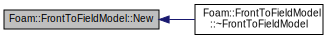
\includegraphics[width=350pt]{classFoam_1_1FrontToFieldModel_a8d2ede4c3699e6e7b24c7491723d576e_icgraph}
\end{center}
\end{figure}
\mbox{\Hypertarget{classFoam_1_1FrontToFieldModel_a7a5035a704385de5435e9668c29c3d89}\label{classFoam_1_1FrontToFieldModel_a7a5035a704385de5435e9668c29c3d89}} 
\index{Foam\+::\+Front\+To\+Field\+Model@{Foam\+::\+Front\+To\+Field\+Model}!two\+Fluid\+Flow@{two\+Fluid\+Flow}}
\index{two\+Fluid\+Flow@{two\+Fluid\+Flow}!Foam\+::\+Front\+To\+Field\+Model@{Foam\+::\+Front\+To\+Field\+Model}}
\subsubsection{\texorpdfstring{two\+Fluid\+Flow()}{twoFluidFlow()}\hspace{0.1cm}{\footnotesize\ttfamily [1/2]}}
{\footnotesize\ttfamily template$<$class Cloud\+Type$>$ \\
bool \hyperlink{classFoam_1_1FrontToFieldModel}{Foam\+::\+Front\+To\+Field\+Model}$<$ Cloud\+Type $>$\+::two\+Fluid\+Flow (\begin{DoxyParamCaption}{ }\end{DoxyParamCaption}) const\hspace{0.3cm}{\ttfamily [inline]}}

\mbox{\Hypertarget{classFoam_1_1FrontToFieldModel_a7a5035a704385de5435e9668c29c3d89}\label{classFoam_1_1FrontToFieldModel_a7a5035a704385de5435e9668c29c3d89}} 
\index{Foam\+::\+Front\+To\+Field\+Model@{Foam\+::\+Front\+To\+Field\+Model}!two\+Fluid\+Flow@{two\+Fluid\+Flow}}
\index{two\+Fluid\+Flow@{two\+Fluid\+Flow}!Foam\+::\+Front\+To\+Field\+Model@{Foam\+::\+Front\+To\+Field\+Model}}
\subsubsection{\texorpdfstring{two\+Fluid\+Flow()}{twoFluidFlow()}\hspace{0.1cm}{\footnotesize\ttfamily [2/2]}}
{\footnotesize\ttfamily template$<$class Cloud\+Type $>$ \\
bool \hyperlink{classFoam_1_1FrontToFieldModel}{Foam\+::\+Front\+To\+Field\+Model}$<$ Cloud\+Type $>$\+::two\+Fluid\+Flow (\begin{DoxyParamCaption}{ }\end{DoxyParamCaption}) const\hspace{0.3cm}{\ttfamily [inline]}}

\mbox{\Hypertarget{classFoam_1_1FrontToFieldModel_a6e113da5c0c612fe1313cffc439e44e9}\label{classFoam_1_1FrontToFieldModel_a6e113da5c0c612fe1313cffc439e44e9}} 
\index{Foam\+::\+Front\+To\+Field\+Model@{Foam\+::\+Front\+To\+Field\+Model}!Type\+Name@{Type\+Name}}
\index{Type\+Name@{Type\+Name}!Foam\+::\+Front\+To\+Field\+Model@{Foam\+::\+Front\+To\+Field\+Model}}
\subsubsection{\texorpdfstring{Type\+Name()}{TypeName()}\hspace{0.1cm}{\footnotesize\ttfamily [1/2]}}
{\footnotesize\ttfamily template$<$class Cloud\+Type$>$ \\
\hyperlink{classFoam_1_1FrontToFieldModel}{Foam\+::\+Front\+To\+Field\+Model}$<$ Cloud\+Type $>$\+::Type\+Name (\begin{DoxyParamCaption}\item[{\char`\"{}front\+To\+Field\+Model\char`\"{}}]{ }\end{DoxyParamCaption})}

\mbox{\Hypertarget{classFoam_1_1FrontToFieldModel_a6e113da5c0c612fe1313cffc439e44e9}\label{classFoam_1_1FrontToFieldModel_a6e113da5c0c612fe1313cffc439e44e9}} 
\index{Foam\+::\+Front\+To\+Field\+Model@{Foam\+::\+Front\+To\+Field\+Model}!Type\+Name@{Type\+Name}}
\index{Type\+Name@{Type\+Name}!Foam\+::\+Front\+To\+Field\+Model@{Foam\+::\+Front\+To\+Field\+Model}}
\subsubsection{\texorpdfstring{Type\+Name()}{TypeName()}\hspace{0.1cm}{\footnotesize\ttfamily [2/2]}}
{\footnotesize\ttfamily template$<$class Cloud\+Type$>$ \\
\hyperlink{classFoam_1_1FrontToFieldModel}{Foam\+::\+Front\+To\+Field\+Model}$<$ Cloud\+Type $>$\+::Type\+Name (\begin{DoxyParamCaption}\item[{\char`\"{}front\+To\+Field\+Model\char`\"{}}]{ }\end{DoxyParamCaption})}

\mbox{\Hypertarget{classFoam_1_1FrontToFieldModel_aab2ed845099ce21bb0c3ab7ac0ac35c5}\label{classFoam_1_1FrontToFieldModel_aab2ed845099ce21bb0c3ab7ac0ac35c5}} 
\index{Foam\+::\+Front\+To\+Field\+Model@{Foam\+::\+Front\+To\+Field\+Model}!viscosity\+Indicator@{viscosity\+Indicator}}
\index{viscosity\+Indicator@{viscosity\+Indicator}!Foam\+::\+Front\+To\+Field\+Model@{Foam\+::\+Front\+To\+Field\+Model}}
\subsubsection{\texorpdfstring{viscosity\+Indicator()}{viscosityIndicator()}\hspace{0.1cm}{\footnotesize\ttfamily [1/2]}}
{\footnotesize\ttfamily template$<$class Cloud\+Type$>$ \\
tmp$<$vol\+Scalar\+Field$>$ \hyperlink{classFoam_1_1FrontToFieldModel}{Foam\+::\+Front\+To\+Field\+Model}$<$ Cloud\+Type $>$\+::viscosity\+Indicator (\begin{DoxyParamCaption}{ }\end{DoxyParamCaption}) const\hspace{0.3cm}{\ttfamily [inline]}}

\mbox{\Hypertarget{classFoam_1_1FrontToFieldModel_acd7d5c4007bd82eec12e23b6e7c0e6a4}\label{classFoam_1_1FrontToFieldModel_acd7d5c4007bd82eec12e23b6e7c0e6a4}} 
\index{Foam\+::\+Front\+To\+Field\+Model@{Foam\+::\+Front\+To\+Field\+Model}!viscosity\+Indicator@{viscosity\+Indicator}}
\index{viscosity\+Indicator@{viscosity\+Indicator}!Foam\+::\+Front\+To\+Field\+Model@{Foam\+::\+Front\+To\+Field\+Model}}
\subsubsection{\texorpdfstring{viscosity\+Indicator()}{viscosityIndicator()}\hspace{0.1cm}{\footnotesize\ttfamily [2/2]}}
{\footnotesize\ttfamily template$<$class Cloud\+Type $>$ \\
Foam\+::tmp$<$ Foam\+::vol\+Scalar\+Field $>$ \hyperlink{classFoam_1_1FrontToFieldModel}{Foam\+::\+Front\+To\+Field\+Model}$<$ Cloud\+Type $>$\+::viscosity\+Indicator (\begin{DoxyParamCaption}{ }\end{DoxyParamCaption}) const\hspace{0.3cm}{\ttfamily [inline]}}

\mbox{\Hypertarget{classFoam_1_1FrontToFieldModel_a36a55af8f324d11462adfacaf082b75b}\label{classFoam_1_1FrontToFieldModel_a36a55af8f324d11462adfacaf082b75b}} 
\index{Foam\+::\+Front\+To\+Field\+Model@{Foam\+::\+Front\+To\+Field\+Model}!viscosity\+Indicator\+Ref@{viscosity\+Indicator\+Ref}}
\index{viscosity\+Indicator\+Ref@{viscosity\+Indicator\+Ref}!Foam\+::\+Front\+To\+Field\+Model@{Foam\+::\+Front\+To\+Field\+Model}}
\subsubsection{\texorpdfstring{viscosity\+Indicator\+Ref()}{viscosityIndicatorRef()}\hspace{0.1cm}{\footnotesize\ttfamily [1/2]}}
{\footnotesize\ttfamily template$<$class Cloud\+Type $>$ \\
Foam\+::vol\+Scalar\+Field \& \hyperlink{classFoam_1_1FrontToFieldModel}{Foam\+::\+Front\+To\+Field\+Model}$<$ Cloud\+Type $>$\+::viscosity\+Indicator\+Ref (\begin{DoxyParamCaption}{ }\end{DoxyParamCaption})\hspace{0.3cm}{\ttfamily [inline]}}

\mbox{\Hypertarget{classFoam_1_1FrontToFieldModel_a473af3afa64c2a730b7c6a6c067708e8}\label{classFoam_1_1FrontToFieldModel_a473af3afa64c2a730b7c6a6c067708e8}} 
\index{Foam\+::\+Front\+To\+Field\+Model@{Foam\+::\+Front\+To\+Field\+Model}!viscosity\+Indicator\+Ref@{viscosity\+Indicator\+Ref}}
\index{viscosity\+Indicator\+Ref@{viscosity\+Indicator\+Ref}!Foam\+::\+Front\+To\+Field\+Model@{Foam\+::\+Front\+To\+Field\+Model}}
\subsubsection{\texorpdfstring{viscosity\+Indicator\+Ref()}{viscosityIndicatorRef()}\hspace{0.1cm}{\footnotesize\ttfamily [2/2]}}
{\footnotesize\ttfamily template$<$class Cloud\+Type$>$ \\
vol\+Scalar\+Field\& \hyperlink{classFoam_1_1FrontToFieldModel}{Foam\+::\+Front\+To\+Field\+Model}$<$ Cloud\+Type $>$\+::viscosity\+Indicator\+Ref (\begin{DoxyParamCaption}{ }\end{DoxyParamCaption})\hspace{0.3cm}{\ttfamily [inline]}}



\subsection{Member Data Documentation}
\mbox{\Hypertarget{classFoam_1_1FrontToFieldModel_af547073005a760654aa30b6e0fe4d41c}\label{classFoam_1_1FrontToFieldModel_af547073005a760654aa30b6e0fe4d41c}} 
\index{Foam\+::\+Front\+To\+Field\+Model@{Foam\+::\+Front\+To\+Field\+Model}!cells\+To\+Refine\+\_\+@{cells\+To\+Refine\+\_\+}}
\index{cells\+To\+Refine\+\_\+@{cells\+To\+Refine\+\_\+}!Foam\+::\+Front\+To\+Field\+Model@{Foam\+::\+Front\+To\+Field\+Model}}
\subsubsection{\texorpdfstring{cells\+To\+Refine\+\_\+}{cellsToRefine\_}}
{\footnotesize\ttfamily template$<$class Cloud\+Type$>$ \\
vol\+Scalar\+Field \hyperlink{classFoam_1_1FrontToFieldModel}{Foam\+::\+Front\+To\+Field\+Model}$<$ Cloud\+Type $>$\+::cells\+To\+Refine\+\_\+}

\mbox{\Hypertarget{classFoam_1_1FrontToFieldModel_a401f7fb4cf5ca62b7a333f9fa8dd89d7}\label{classFoam_1_1FrontToFieldModel_a401f7fb4cf5ca62b7a333f9fa8dd89d7}} 
\index{Foam\+::\+Front\+To\+Field\+Model@{Foam\+::\+Front\+To\+Field\+Model}!density\+Indicator\+\_\+@{density\+Indicator\+\_\+}}
\index{density\+Indicator\+\_\+@{density\+Indicator\+\_\+}!Foam\+::\+Front\+To\+Field\+Model@{Foam\+::\+Front\+To\+Field\+Model}}
\subsubsection{\texorpdfstring{density\+Indicator\+\_\+}{densityIndicator\_}}
{\footnotesize\ttfamily template$<$class Cloud\+Type$>$ \\
auto\+Ptr$<$ vol\+Scalar\+Field $>$ \hyperlink{classFoam_1_1FrontToFieldModel}{Foam\+::\+Front\+To\+Field\+Model}$<$ Cloud\+Type $>$\+::density\+Indicator\+\_\+}

\mbox{\Hypertarget{classFoam_1_1FrontToFieldModel_a2eca985c837b4173dae0ab002b512c91}\label{classFoam_1_1FrontToFieldModel_a2eca985c837b4173dae0ab002b512c91}} 
\index{Foam\+::\+Front\+To\+Field\+Model@{Foam\+::\+Front\+To\+Field\+Model}!h\+\_\+@{h\+\_\+}}
\index{h\+\_\+@{h\+\_\+}!Foam\+::\+Front\+To\+Field\+Model@{Foam\+::\+Front\+To\+Field\+Model}}
\subsubsection{\texorpdfstring{h\+\_\+}{h\_}}
{\footnotesize\ttfamily template$<$class Cloud\+Type$>$ \\
scalar \hyperlink{classFoam_1_1FrontToFieldModel}{Foam\+::\+Front\+To\+Field\+Model}$<$ Cloud\+Type $>$\+::h\+\_\+}

\mbox{\Hypertarget{classFoam_1_1FrontToFieldModel_a775b7bec736f2ca57e1d03dcd6b7c873}\label{classFoam_1_1FrontToFieldModel_a775b7bec736f2ca57e1d03dcd6b7c873}} 
\index{Foam\+::\+Front\+To\+Field\+Model@{Foam\+::\+Front\+To\+Field\+Model}!h\+Factor\+\_\+@{h\+Factor\+\_\+}}
\index{h\+Factor\+\_\+@{h\+Factor\+\_\+}!Foam\+::\+Front\+To\+Field\+Model@{Foam\+::\+Front\+To\+Field\+Model}}
\subsubsection{\texorpdfstring{h\+Factor\+\_\+}{hFactor\_}}
{\footnotesize\ttfamily template$<$class Cloud\+Type$>$ \\
scalar \hyperlink{classFoam_1_1FrontToFieldModel}{Foam\+::\+Front\+To\+Field\+Model}$<$ Cloud\+Type $>$\+::h\+Factor\+\_\+}

\mbox{\Hypertarget{classFoam_1_1FrontToFieldModel_a95395337010439fe57e0ecc9ca2bb23a}\label{classFoam_1_1FrontToFieldModel_a95395337010439fe57e0ecc9ca2bb23a}} 
\index{Foam\+::\+Front\+To\+Field\+Model@{Foam\+::\+Front\+To\+Field\+Model}!Indicator\+\_\+@{Indicator\+\_\+}}
\index{Indicator\+\_\+@{Indicator\+\_\+}!Foam\+::\+Front\+To\+Field\+Model@{Foam\+::\+Front\+To\+Field\+Model}}
\subsubsection{\texorpdfstring{Indicator\+\_\+}{Indicator\_}}
{\footnotesize\ttfamily template$<$class Cloud\+Type$>$ \\
auto\+Ptr$<$ vol\+Scalar\+Field $>$ \hyperlink{classFoam_1_1FrontToFieldModel}{Foam\+::\+Front\+To\+Field\+Model}$<$ Cloud\+Type $>$\+::Indicator\+\_\+}

\mbox{\Hypertarget{classFoam_1_1FrontToFieldModel_ad04fa93b89f90606f8f0f0111e29aef7}\label{classFoam_1_1FrontToFieldModel_ad04fa93b89f90606f8f0f0111e29aef7}} 
\index{Foam\+::\+Front\+To\+Field\+Model@{Foam\+::\+Front\+To\+Field\+Model}!two\+Fluid\+Flow\+\_\+@{two\+Fluid\+Flow\+\_\+}}
\index{two\+Fluid\+Flow\+\_\+@{two\+Fluid\+Flow\+\_\+}!Foam\+::\+Front\+To\+Field\+Model@{Foam\+::\+Front\+To\+Field\+Model}}
\subsubsection{\texorpdfstring{two\+Fluid\+Flow\+\_\+}{twoFluidFlow\_}}
{\footnotesize\ttfamily template$<$class Cloud\+Type$>$ \\
bool \hyperlink{classFoam_1_1FrontToFieldModel}{Foam\+::\+Front\+To\+Field\+Model}$<$ Cloud\+Type $>$\+::two\+Fluid\+Flow\+\_\+}

\mbox{\Hypertarget{classFoam_1_1FrontToFieldModel_ace19a4b367734365c6e4367def23a06e}\label{classFoam_1_1FrontToFieldModel_ace19a4b367734365c6e4367def23a06e}} 
\index{Foam\+::\+Front\+To\+Field\+Model@{Foam\+::\+Front\+To\+Field\+Model}!viscosity\+Indicator\+\_\+@{viscosity\+Indicator\+\_\+}}
\index{viscosity\+Indicator\+\_\+@{viscosity\+Indicator\+\_\+}!Foam\+::\+Front\+To\+Field\+Model@{Foam\+::\+Front\+To\+Field\+Model}}
\subsubsection{\texorpdfstring{viscosity\+Indicator\+\_\+}{viscosityIndicator\_}}
{\footnotesize\ttfamily template$<$class Cloud\+Type$>$ \\
auto\+Ptr$<$ vol\+Scalar\+Field $>$ \hyperlink{classFoam_1_1FrontToFieldModel}{Foam\+::\+Front\+To\+Field\+Model}$<$ Cloud\+Type $>$\+::viscosity\+Indicator\+\_\+}



The documentation for this class was generated from the following files\+:\begin{DoxyCompactItemize}
\item 
clouds/\+Templates/\+Front\+Tracking\+Cloud/\hyperlink{clouds_2Templates_2FrontTrackingCloud_2FrontTrackingCloud_8H}{Front\+Tracking\+Cloud.\+H}\item 
ln\+Include/\hyperlink{lnInclude_2FrontToFieldModel_8H}{Front\+To\+Field\+Model.\+H}\item 
ln\+Include/\hyperlink{lnInclude_2FrontToFieldModel_8C}{Front\+To\+Field\+Model.\+C}\end{DoxyCompactItemize}

\hypertarget{classFoam_1_1FrontTrackingCloud}{}\section{Foam\+:\+:Front\+Tracking\+Cloud$<$ Cloud\+Type $>$ Class Template Reference}
\label{classFoam_1_1FrontTrackingCloud}\index{Foam\+::\+Front\+Tracking\+Cloud$<$ Cloud\+Type $>$@{Foam\+::\+Front\+Tracking\+Cloud$<$ Cloud\+Type $>$}}


{\ttfamily \#include $<$Front\+Tracking\+Cloud.\+H$>$}



Inheritance diagram for Foam\+:\+:Front\+Tracking\+Cloud$<$ Cloud\+Type $>$\+:\nopagebreak
\begin{figure}[H]
\begin{center}
\leavevmode
\includegraphics[height=550pt]{classFoam_1_1FrontTrackingCloud__inherit__graph}
\end{center}
\end{figure}


Collaboration diagram for Foam\+:\+:Front\+Tracking\+Cloud$<$ Cloud\+Type $>$\+:\nopagebreak
\begin{figure}[H]
\begin{center}
\leavevmode
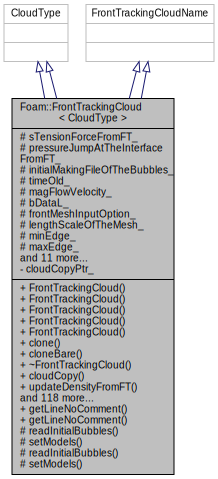
\includegraphics[height=550pt]{classFoam_1_1FrontTrackingCloud__coll__graph}
\end{center}
\end{figure}
\subsection*{Public Types}
\begin{DoxyCompactItemize}
\item 
typedef Cloud\+Type \hyperlink{classFoam_1_1FrontTrackingCloud_aa902341b7e8a28b529bd81515b13b5a6}{cloud\+Type}
\item 
typedef Cloud\+Type\+::parcel\+Type \hyperlink{classFoam_1_1FrontTrackingCloud_a18be05626026eec2bf2a990da073a350}{parcel\+Type}
\item 
typedef \hyperlink{classFoam_1_1FrontTrackingCloud}{Front\+Tracking\+Cloud}$<$ Cloud\+Type $>$ \hyperlink{classFoam_1_1FrontTrackingCloud_a2a9868cc5ecf74928b8ac51ee41e659d}{Front\+Tracking\+Cloud\+Type}
\item 
typedef Cloud\+Type \hyperlink{classFoam_1_1FrontTrackingCloud_aa902341b7e8a28b529bd81515b13b5a6}{cloud\+Type}
\item 
typedef Cloud\+Type\+::parcel\+Type \hyperlink{classFoam_1_1FrontTrackingCloud_a18be05626026eec2bf2a990da073a350}{parcel\+Type}
\item 
typedef \hyperlink{classFoam_1_1FrontTrackingCloud}{Front\+Tracking\+Cloud}$<$ Cloud\+Type $>$ \hyperlink{classFoam_1_1FrontTrackingCloud_a2a9868cc5ecf74928b8ac51ee41e659d}{Front\+Tracking\+Cloud\+Type}
\end{DoxyCompactItemize}
\subsection*{Public Member Functions}
\begin{DoxyCompactItemize}
\item 
\hyperlink{classFoam_1_1FrontTrackingCloud_ae9da3f76099b9b82be67cf99ae64ab28}{Front\+Tracking\+Cloud} (const word \&cloud\+Name, const vol\+Scalar\+Field \&rho, const vol\+Vector\+Field \&U, const vol\+Scalar\+Field \&mu, const dimensioned\+Vector \&g, const bool read\+Fields=true)
\item 
\hyperlink{classFoam_1_1FrontTrackingCloud_ad185ad598e5280fdea20a85d8aff1e91}{Front\+Tracking\+Cloud} (const word \&cloud\+Name, const vol\+Scalar\+Field \&rho, const vol\+Vector\+Field \&U, const dimensioned\+Vector \&g, const fluid\+Thermo \&carrier\+Thermo, const bool read\+Fields=true)
\item 
\hyperlink{classFoam_1_1FrontTrackingCloud_aaf498c2097937a9147685bd0de6a85bb}{Front\+Tracking\+Cloud} (\hyperlink{classFoam_1_1FrontTrackingCloud}{Front\+Tracking\+Cloud}$<$ Cloud\+Type $>$ \&c, const word \&name)
\item 
\hyperlink{classFoam_1_1FrontTrackingCloud_a87899dfd5f7408b0da887eafe1fb2a43}{Front\+Tracking\+Cloud} (const fv\+Mesh \&mesh, const word \&name, const \hyperlink{classFoam_1_1FrontTrackingCloud}{Front\+Tracking\+Cloud}$<$ Cloud\+Type $>$ \&c)
\item 
\hyperlink{classFoam_1_1FrontTrackingCloud_ac8860f6c62a4086d2cc0d00e28ed88de}{Front\+Tracking\+Cloud} (const \hyperlink{classFoam_1_1FrontTrackingCloud}{Front\+Tracking\+Cloud} \&)=delete
\item 
virtual auto\+Ptr$<$ Cloud$<$ \hyperlink{classFoam_1_1FrontTrackingCloud_a18be05626026eec2bf2a990da073a350}{parcel\+Type} $>$ $>$ \hyperlink{classFoam_1_1FrontTrackingCloud_ad82d33465c7a25d3d72f5ec29707edd4}{clone} (const word \&name)
\item 
virtual auto\+Ptr$<$ Cloud$<$ \hyperlink{classFoam_1_1FrontTrackingCloud_a18be05626026eec2bf2a990da073a350}{parcel\+Type} $>$ $>$ \hyperlink{classFoam_1_1FrontTrackingCloud_aaee595291402fafdae131c72fe7c8a38}{clone\+Bare} (const word \&name) const
\item 
virtual \hyperlink{classFoam_1_1FrontTrackingCloud_a8aaede4a1c43afed7a499fdbe20ba62a}{$\sim$\+Front\+Tracking\+Cloud} ()
\item 
const \hyperlink{classFoam_1_1FrontTrackingCloud}{Front\+Tracking\+Cloud} \& \hyperlink{classFoam_1_1FrontTrackingCloud_a5de0cfc162d5fca7f01c09bec6484a80}{cloud\+Copy} () const
\item 
void \hyperlink{classFoam_1_1FrontTrackingCloud_aa56916fe7ca5b51f58aebb1579733ce7}{update\+Density\+From\+FT} (vol\+Scalar\+Field \&rho)
\item 
void \hyperlink{classFoam_1_1FrontTrackingCloud_a431fe5f20e5f9f9de43b1ffa7d208504}{update\+Viscosity\+From\+FT} (vol\+Scalar\+Field \&mu)
\item 
vol\+Vector\+Field\+::\+Internal \& \hyperlink{classFoam_1_1FrontTrackingCloud_ad53ea56fc9ffc915c31829cca0ea31db}{s\+Tension\+Force\+From\+F\+T\+Ref} ()
\item 
tmp$<$ vol\+Vector\+Field\+::\+Internal $>$ \hyperlink{classFoam_1_1FrontTrackingCloud_a0ae6d786992668f3b1c4d95eb793b9e7}{s\+Tension\+Force\+From\+FT} () const
\item 
vol\+Vector\+Field\+::\+Internal \& \hyperlink{classFoam_1_1FrontTrackingCloud_a96c2b9704ee7cead115cca5df4556e78}{pressure\+Jump\+At\+The\+Interface\+From\+F\+T\+Ref} ()
\item 
tmp$<$ vol\+Vector\+Field\+::\+Internal $>$ \hyperlink{classFoam_1_1FrontTrackingCloud_a670a8c0837d0b52b671eb2df4689dfb2}{pressure\+Jump\+At\+The\+Interface\+From\+FT} () const
\item 
const \hyperlink{classFoam_1_1SurfaceTensionModel}{Surface\+Tension\+Model}$<$ \hyperlink{classFoam_1_1FrontTrackingCloud}{Front\+Tracking\+Cloud}$<$ Cloud\+Type $>$ $>$ \& \hyperlink{classFoam_1_1FrontTrackingCloud_a5b19489cbba64adfe1ac441f1415b5ac}{surface\+Tension\+Model} () const
\item 
\hyperlink{classFoam_1_1SurfaceTensionModel}{Surface\+Tension\+Model}$<$ \hyperlink{classFoam_1_1FrontTrackingCloud}{Front\+Tracking\+Cloud}$<$ Cloud\+Type $>$ $>$ \& \hyperlink{classFoam_1_1FrontTrackingCloud_a5caa79e8ad33026aeb369369f5e20803}{surface\+Tension\+Model} ()
\item 
const \hyperlink{classFoam_1_1FrontToFieldModel}{Front\+To\+Field\+Model}$<$ \hyperlink{classFoam_1_1FrontTrackingCloud}{Front\+Tracking\+Cloud}$<$ Cloud\+Type $>$ $>$ \& \hyperlink{classFoam_1_1FrontTrackingCloud_a96c6c87cd96ab04e16913b7c9738e83b}{front\+To\+Field\+Model} () const
\item 
\hyperlink{classFoam_1_1FrontToFieldModel}{Front\+To\+Field\+Model}$<$ \hyperlink{classFoam_1_1FrontTrackingCloud}{Front\+Tracking\+Cloud}$<$ Cloud\+Type $>$ $>$ \& \hyperlink{classFoam_1_1FrontTrackingCloud_a1647e6f7debf6dd01efce9e35d213508}{front\+To\+Field\+Model} ()
\item 
const \hyperlink{classFoam_1_1VolumeCorrectionModel}{Volume\+Correction\+Model}$<$ \hyperlink{classFoam_1_1FrontTrackingCloud}{Front\+Tracking\+Cloud}$<$ Cloud\+Type $>$ $>$ \& \hyperlink{classFoam_1_1FrontTrackingCloud_a13e331ab53bd43354e7d106bd6d1e66e}{volume\+Correction\+Model} () const
\item 
\hyperlink{classFoam_1_1VolumeCorrectionModel}{Volume\+Correction\+Model}$<$ \hyperlink{classFoam_1_1FrontTrackingCloud}{Front\+Tracking\+Cloud}$<$ Cloud\+Type $>$ $>$ \& \hyperlink{classFoam_1_1FrontTrackingCloud_a64d9bd3b8314e7e00da69f5ba862258f}{volume\+Correction\+Model} ()
\item 
const \hyperlink{classFoam_1_1UndulationRemovalModel}{Undulation\+Removal\+Model}$<$ \hyperlink{classFoam_1_1FrontTrackingCloud}{Front\+Tracking\+Cloud}$<$ Cloud\+Type $>$ $>$ \& \hyperlink{classFoam_1_1FrontTrackingCloud_a1d06be478c0ca9d2f7835f7c6a9b375e}{undulation\+Removal\+Model} () const
\item 
\hyperlink{classFoam_1_1UndulationRemovalModel}{Undulation\+Removal\+Model}$<$ \hyperlink{classFoam_1_1FrontTrackingCloud}{Front\+Tracking\+Cloud}$<$ Cloud\+Type $>$ $>$ \& \hyperlink{classFoam_1_1FrontTrackingCloud_a8c60743be0c8eab0391134f1b4206781}{undulation\+Removal\+Model} ()
\item 
const Dynamic\+List$<$ \hyperlink{classFoam_1_1bubbleData}{bubble\+Data} $>$ \& \hyperlink{classFoam_1_1FrontTrackingCloud_a2facef866c2c46b20c00baf6e2836df8}{b\+DataL} () const
\item 
Dynamic\+List$<$ \hyperlink{classFoam_1_1bubbleData}{bubble\+Data} $>$ \& \hyperlink{classFoam_1_1FrontTrackingCloud_ad609a644410a3223f9c6e089f491ad33}{b\+DataL} ()
\item 
scalar \hyperlink{classFoam_1_1FrontTrackingCloud_a7198b91c55f61b2544380d2696c785d2}{length\+Scale\+Of\+The\+Mesh} () const
\item 
List$<$ Dynamic\+List$<$ label $>$ $>$ \hyperlink{classFoam_1_1FrontTrackingCloud_a3cc5fbc7520219ddd33f6bc589722b82}{all\+Cells\+In\+Eeach\+Masket} () const
\item 
List$<$ scalar $>$ \hyperlink{classFoam_1_1FrontTrackingCloud_afb318a2851b231842c8c45b5efd11724}{length\+Scale\+Near\+The\+Front} () const
\item 
void \hyperlink{classFoam_1_1FrontTrackingCloud_ab42c0d5842ebbe4deef24d207c1f6a44}{store\+State} ()
\item 
void \hyperlink{classFoam_1_1FrontTrackingCloud_a32db2743973df01d6e8b509ffcbcab23}{restore\+State} ()
\item 
void \hyperlink{classFoam_1_1FrontTrackingCloud_a250cbdc0d51e8b7a90e341bd2e78b877}{evolve} ()
\item 
{\footnotesize template$<$class Track\+Cloud\+Type $>$ }\\void \hyperlink{classFoam_1_1FrontTrackingCloud_a88a815f4b61ca82999166c43accda650}{motion} (Track\+Cloud\+Type \&cloud, typename parcel\+Type\+::tracking\+Data \&td)
\item 
void \hyperlink{classFoam_1_1FrontTrackingCloud_ab56e418175f86982ef3b36c6e74e4fdc}{cloud\+Cleaning} ()
\item 
void \hyperlink{classFoam_1_1FrontTrackingCloud_adf887a6c3490e9ab5d11566713b35386}{map\+Front\+To\+Parcel} ()
\item 
{\footnotesize template$<$class Track\+Cloud\+Type $>$ }\\void \hyperlink{classFoam_1_1FrontTrackingCloud_a6a3db7a4b4111c52f10a81f56b2b2429}{update\+Parcels\+From\+Front} (Track\+Cloud\+Type \&cloud, typename parcel\+Type\+::tracking\+Data \&td)
\item 
{\footnotesize template$<$class Track\+Cloud\+Type $>$ }\\void \hyperlink{classFoam_1_1FrontTrackingCloud_a07213caaa12b062cf109d5e1c787bd7b}{front\+Cloud\+Advection} (Track\+Cloud\+Type \&cloud, typename parcel\+Type\+::tracking\+Data \&td)
\item 
void \hyperlink{classFoam_1_1FrontTrackingCloud_a1b7c9f2c13ef22253a0ffc6610b62c09}{map\+Point\+To\+Parcel} (label b\+DI, \hyperlink{classFoam_1_1pointData}{point\+Data} \&ptD)
\item 
void \hyperlink{classFoam_1_1FrontTrackingCloud_a5719f87b5899aa9675daf150a997f37a}{constructing\+Initial\+Front} ()
\item 
void \hyperlink{classFoam_1_1FrontTrackingCloud_a356c54185b3b13a1b75a8400e2676cf7}{read\+Data\+Of\+The\+Fronts\+At\+The\+Current\+Time\+Intime\+Name} ()
\item 
Foam\+::scalar \hyperlink{classFoam_1_1FrontTrackingCloud_aa8d4bc5e201416b5b147c184c11940df}{calc\+Length\+Scale\+Of\+The\+Mesh} ()
\item 
void \hyperlink{classFoam_1_1FrontTrackingCloud_a7122d2164461e7766c0aa1a101814944}{set\+Length\+Scales\+Near\+The\+Front} ()
\item 
void \hyperlink{classFoam_1_1FrontTrackingCloud_ab7706a4a237ef93320cf8194480a4847}{communications\+Of\+The\+Front\+And\+Eulerian\+Grid} ()
\item 
void \hyperlink{classFoam_1_1FrontTrackingCloud_ad891f47822721d3da1f015da2800df7c}{search\+All\+Cells\+In\+Eeach\+Masket} ()
\item 
void \hyperlink{classFoam_1_1FrontTrackingCloud_a0bb2522d2ddf9404386ba4b5a5a288ee}{processing\+Thefront\+Meshes} ()
\item 
void \hyperlink{classFoam_1_1FrontTrackingCloud_ab2c887bd558ca828970699810da950fb}{update\+Pl\+Pos\+In\+Domain} (\hyperlink{classFoam_1_1bubbleData}{bubble\+Data} \&b\+Data)
\item 
void \hyperlink{classFoam_1_1FrontTrackingCloud_aa6fe428d5f06ec56363494e50dcddbef}{update\+El\+Centre\+Pos\+In\+Domain} (\hyperlink{classFoam_1_1bubbleData}{bubble\+Data} \&b\+Data)
\item 
void \hyperlink{classFoam_1_1FrontTrackingCloud_ada5f5e05db21f49b7d61c74fecc37db0}{adjusting\+The\+Cloud\+Data\+After\+Changes} (label\+List \&loc\+In\+Point\+Data\+List, label b\+DI)
\item 
void \hyperlink{classFoam_1_1FrontTrackingCloud_af71f0286cb6f689c9aa0e392b4ca8eca}{front\+Refining} (label b\+DI, Dynamic\+List$<$ \hyperlink{classFoam_1_1pointData}{point\+Data} $>$ \&pt\+Data\+List, Dynamic\+List$<$ \hyperlink{classFoam_1_1elementInfo}{element\+Info} $>$ \&el\+Info\+List, scalar min\+Edge, scalar max\+Edge, scalar max\+Aspect\+Ratio)
\item 
bool \hyperlink{classFoam_1_1FrontTrackingCloud_acd0406a159d2deeccb2b112fdbb9d3ca}{is\+Element\+Small} (\hyperlink{classFoam_1_1elementInfo}{element\+Info} el, scalar min\+Edge, scalar max\+Edge, scalar max\+Aspect\+Ratio, scalar \&s1, scalar \&s2, scalar \&s3, label \&n1, label \&n2, label \&n3)
\item 
bool \hyperlink{classFoam_1_1FrontTrackingCloud_a10b7243bf15e0edbac31b1a32d226237}{is\+Element\+Refined} (\hyperlink{classFoam_1_1elementInfo}{element\+Info} el, scalar min\+Edge, scalar max\+Edge, scalar max\+Aspect\+Ratio, scalar \&s1, scalar \&s2, scalar \&s3, label \&n1, label \&n2, label \&n3)
\item 
void \hyperlink{classFoam_1_1FrontTrackingCloud_af6a86830e32ecf4700c0dfe908f8455b}{front\+Coarsening} (label b\+DI, Dynamic\+List$<$ \hyperlink{classFoam_1_1pointData}{point\+Data} $>$ \&pt\+Data\+List, Dynamic\+List$<$ \hyperlink{classFoam_1_1elementInfo}{element\+Info} $>$ \&el\+Info\+List, scalar min\+Edge, scalar max\+Edge, scalar max\+Aspect\+Ratio)
\item 
void \hyperlink{classFoam_1_1FrontTrackingCloud_a147fdd88043c9633e0591711c040ed86}{map\+Parcel\+To\+Front} ()
\item 
void \hyperlink{classFoam_1_1FrontTrackingCloud_a4454726d277c31c277cfabb11b37dfa5}{set\+Motion\+Flags} ()
\item 
void \hyperlink{classFoam_1_1FrontTrackingCloud_a2c98143d36515d589f04cd973de83edc}{set\+C\+R\+Flags} ()
\item 
void \hyperlink{classFoam_1_1FrontTrackingCloud_a94e1d0ebd73a8a41a79f0c178ca51e9d}{printing\+All\+Important\+Run\+Time\+Data} ()
\item 
void \hyperlink{classFoam_1_1FrontTrackingCloud_ad5f38cae41120ba49f55c71ae46e6323}{output\+Time\+Post\+Processing} ()
\item 
void \hyperlink{classFoam_1_1FrontTrackingCloud_a9d5d59f9f43a2a45c8788b0cc3e9ea0b}{bubble\+Post\+Processing} ()
\item 
void \hyperlink{classFoam_1_1FrontTrackingCloud_ac141c7f5cca70abc443c730c2ce48720}{write\+Bubble\+Positions} ()
\item 
void \hyperlink{classFoam_1_1FrontTrackingCloud_ae0c2a7df61bf67ddecc30b59c8606010}{write\+Bubble\+Velocity\+And\+Accelaration} ()
\item 
void \hyperlink{classFoam_1_1FrontTrackingCloud_ab5c55ecf9166e47afc104f89d9aaed02}{write\+Bubble\+Sphericity} ()
\item 
void \hyperlink{classFoam_1_1FrontTrackingCloud_a5637e3be2d96f505313e700e31d96d3f}{calc\+Bubble\+Non\+Dimensional\+Numbers} ()
\item 
void \hyperlink{classFoam_1_1FrontTrackingCloud_ac41e53c2edf0af4d0194555602435a5d}{print\+Fronts\+For\+All\+Times} ()
\item 
void \hyperlink{classFoam_1_1FrontTrackingCloud_a5efc9601f8386505e595ed22cf7e425f}{write\+Data\+Of\+The\+Fronts\+At\+The\+Output\+Time\+Intime\+Name} ()
\item 
void \hyperlink{classFoam_1_1FrontTrackingCloud_a82ef9c3e72fcdb1bef553503dc773705}{operator=} (const \hyperlink{classFoam_1_1FrontTrackingCloud}{Front\+Tracking\+Cloud} \&)=delete
\item 
\hyperlink{classFoam_1_1FrontTrackingCloud_ae9da3f76099b9b82be67cf99ae64ab28}{Front\+Tracking\+Cloud} (const word \&cloud\+Name, const vol\+Scalar\+Field \&rho, const vol\+Vector\+Field \&U, const vol\+Scalar\+Field \&mu, const dimensioned\+Vector \&g, const bool read\+Fields=true)
\item 
\hyperlink{classFoam_1_1FrontTrackingCloud_ad185ad598e5280fdea20a85d8aff1e91}{Front\+Tracking\+Cloud} (const word \&cloud\+Name, const vol\+Scalar\+Field \&rho, const vol\+Vector\+Field \&U, const dimensioned\+Vector \&g, const fluid\+Thermo \&carrier\+Thermo, const bool read\+Fields=true)
\item 
\hyperlink{classFoam_1_1FrontTrackingCloud_aaf498c2097937a9147685bd0de6a85bb}{Front\+Tracking\+Cloud} (\hyperlink{classFoam_1_1FrontTrackingCloud}{Front\+Tracking\+Cloud}$<$ Cloud\+Type $>$ \&c, const word \&name)
\item 
\hyperlink{classFoam_1_1FrontTrackingCloud_a87899dfd5f7408b0da887eafe1fb2a43}{Front\+Tracking\+Cloud} (const fv\+Mesh \&mesh, const word \&name, const \hyperlink{classFoam_1_1FrontTrackingCloud}{Front\+Tracking\+Cloud}$<$ Cloud\+Type $>$ \&c)
\item 
\hyperlink{classFoam_1_1FrontTrackingCloud_ac8860f6c62a4086d2cc0d00e28ed88de}{Front\+Tracking\+Cloud} (const \hyperlink{classFoam_1_1FrontTrackingCloud}{Front\+Tracking\+Cloud} \&)=delete
\item 
virtual auto\+Ptr$<$ Cloud$<$ \hyperlink{classFoam_1_1FrontTrackingCloud_a18be05626026eec2bf2a990da073a350}{parcel\+Type} $>$ $>$ \hyperlink{classFoam_1_1FrontTrackingCloud_ad82d33465c7a25d3d72f5ec29707edd4}{clone} (const word \&name)
\item 
virtual auto\+Ptr$<$ Cloud$<$ \hyperlink{classFoam_1_1FrontTrackingCloud_a18be05626026eec2bf2a990da073a350}{parcel\+Type} $>$ $>$ \hyperlink{classFoam_1_1FrontTrackingCloud_aaee595291402fafdae131c72fe7c8a38}{clone\+Bare} (const word \&name) const
\item 
virtual \hyperlink{classFoam_1_1FrontTrackingCloud_adcba24981e24cd97517d109b4197d2c8}{$\sim$\+Front\+Tracking\+Cloud} ()
\item 
const \hyperlink{classFoam_1_1FrontTrackingCloud}{Front\+Tracking\+Cloud} \& \hyperlink{classFoam_1_1FrontTrackingCloud_a916ec076f5dac6164f4908e49759d5d3}{cloud\+Copy} () const
\item 
void \hyperlink{classFoam_1_1FrontTrackingCloud_aa56916fe7ca5b51f58aebb1579733ce7}{update\+Density\+From\+FT} (vol\+Scalar\+Field \&rho)
\item 
void \hyperlink{classFoam_1_1FrontTrackingCloud_a431fe5f20e5f9f9de43b1ffa7d208504}{update\+Viscosity\+From\+FT} (vol\+Scalar\+Field \&mu)
\item 
vol\+Vector\+Field\+::\+Internal \& \hyperlink{classFoam_1_1FrontTrackingCloud_a60533eab6ea8ce9ef1a7d3a4751e9f97}{s\+Tension\+Force\+From\+F\+T\+Ref} ()
\item 
tmp$<$ vol\+Vector\+Field\+::\+Internal $>$ \hyperlink{classFoam_1_1FrontTrackingCloud_a02932aae4789fd058874353c721a8418}{s\+Tension\+Force\+From\+FT} () const
\item 
vol\+Vector\+Field\+::\+Internal \& \hyperlink{classFoam_1_1FrontTrackingCloud_a469be911ad5cefdad34c29eb6256f6f7}{pressure\+Jump\+At\+The\+Interface\+From\+F\+T\+Ref} ()
\item 
tmp$<$ vol\+Vector\+Field\+::\+Internal $>$ \hyperlink{classFoam_1_1FrontTrackingCloud_aa10f81f9d39800c7b8a62f5fb6b23c51}{pressure\+Jump\+At\+The\+Interface\+From\+FT} () const
\item 
const \hyperlink{classFoam_1_1SurfaceTensionModel}{Surface\+Tension\+Model}$<$ \hyperlink{classFoam_1_1FrontTrackingCloud}{Front\+Tracking\+Cloud}$<$ Cloud\+Type $>$ $>$ \& \hyperlink{classFoam_1_1FrontTrackingCloud_a1dca4cd978105ce62b3fe4ad3dcdbba6}{surface\+Tension\+Model} () const
\item 
\hyperlink{classFoam_1_1SurfaceTensionModel}{Surface\+Tension\+Model}$<$ \hyperlink{classFoam_1_1FrontTrackingCloud}{Front\+Tracking\+Cloud}$<$ Cloud\+Type $>$ $>$ \& \hyperlink{classFoam_1_1FrontTrackingCloud_abe536bf6a88024005fcbb9aa1daaaa71}{surface\+Tension\+Model} ()
\item 
const \hyperlink{classFoam_1_1FrontToFieldModel}{Front\+To\+Field\+Model}$<$ \hyperlink{classFoam_1_1FrontTrackingCloud}{Front\+Tracking\+Cloud}$<$ Cloud\+Type $>$ $>$ \& \hyperlink{classFoam_1_1FrontTrackingCloud_ad6554ad2acf4fd4b844c6404d65d9e78}{front\+To\+Field\+Model} () const
\item 
\hyperlink{classFoam_1_1FrontToFieldModel}{Front\+To\+Field\+Model}$<$ \hyperlink{classFoam_1_1FrontTrackingCloud}{Front\+Tracking\+Cloud}$<$ Cloud\+Type $>$ $>$ \& \hyperlink{classFoam_1_1FrontTrackingCloud_a09c3a8c132c3bf452d37e8056cd47677}{front\+To\+Field\+Model} ()
\item 
const \hyperlink{classFoam_1_1VolumeCorrectionModel}{Volume\+Correction\+Model}$<$ \hyperlink{classFoam_1_1FrontTrackingCloud}{Front\+Tracking\+Cloud}$<$ Cloud\+Type $>$ $>$ \& \hyperlink{classFoam_1_1FrontTrackingCloud_a77925665dad6d56392702a9273c7d698}{volume\+Correction\+Model} () const
\item 
\hyperlink{classFoam_1_1VolumeCorrectionModel}{Volume\+Correction\+Model}$<$ \hyperlink{classFoam_1_1FrontTrackingCloud}{Front\+Tracking\+Cloud}$<$ Cloud\+Type $>$ $>$ \& \hyperlink{classFoam_1_1FrontTrackingCloud_ae8081308aa2c529f4c5ae6341a28fdeb}{volume\+Correction\+Model} ()
\item 
const \hyperlink{classFoam_1_1UndulationRemovalModel}{Undulation\+Removal\+Model}$<$ \hyperlink{classFoam_1_1FrontTrackingCloud}{Front\+Tracking\+Cloud}$<$ Cloud\+Type $>$ $>$ \& \hyperlink{classFoam_1_1FrontTrackingCloud_a1d06be478c0ca9d2f7835f7c6a9b375e}{undulation\+Removal\+Model} () const
\item 
\hyperlink{classFoam_1_1UndulationRemovalModel}{Undulation\+Removal\+Model}$<$ \hyperlink{classFoam_1_1FrontTrackingCloud}{Front\+Tracking\+Cloud}$<$ Cloud\+Type $>$ $>$ \& \hyperlink{classFoam_1_1FrontTrackingCloud_a8c60743be0c8eab0391134f1b4206781}{undulation\+Removal\+Model} ()
\item 
const Dynamic\+List$<$ \hyperlink{classFoam_1_1bubbleData}{bubble\+Data} $>$ \& \hyperlink{classFoam_1_1FrontTrackingCloud_aad777230d88c98be784780bbdd6ec4d8}{b\+DataL} () const
\item 
Dynamic\+List$<$ \hyperlink{classFoam_1_1bubbleData}{bubble\+Data} $>$ \& \hyperlink{classFoam_1_1FrontTrackingCloud_af54f24334180fe52e27dce8b1496403c}{b\+DataL} ()
\item 
scalar \hyperlink{classFoam_1_1FrontTrackingCloud_a379ccad5883f38e93d65e5f5e69a36b5}{length\+Scale\+Of\+The\+Mesh} () const
\item 
List$<$ Dynamic\+List$<$ label $>$ $>$ \hyperlink{classFoam_1_1FrontTrackingCloud_a64fb8f2d5fe450ed751ec77733f12641}{all\+Cells\+In\+Eeach\+Masket} () const
\item 
List$<$ scalar $>$ \hyperlink{classFoam_1_1FrontTrackingCloud_a550dbea553308b6b30721371bad76748}{length\+Scale\+Near\+The\+Front} () const
\item 
void \hyperlink{classFoam_1_1FrontTrackingCloud_ab42c0d5842ebbe4deef24d207c1f6a44}{store\+State} ()
\item 
void \hyperlink{classFoam_1_1FrontTrackingCloud_a32db2743973df01d6e8b509ffcbcab23}{restore\+State} ()
\item 
void \hyperlink{classFoam_1_1FrontTrackingCloud_a250cbdc0d51e8b7a90e341bd2e78b877}{evolve} ()
\item 
{\footnotesize template$<$class Track\+Cloud\+Type $>$ }\\void \hyperlink{classFoam_1_1FrontTrackingCloud_a88a815f4b61ca82999166c43accda650}{motion} (Track\+Cloud\+Type \&cloud, typename parcel\+Type\+::tracking\+Data \&td)
\item 
void \hyperlink{classFoam_1_1FrontTrackingCloud_ab56e418175f86982ef3b36c6e74e4fdc}{cloud\+Cleaning} ()
\item 
void \hyperlink{classFoam_1_1FrontTrackingCloud_adf887a6c3490e9ab5d11566713b35386}{map\+Front\+To\+Parcel} ()
\item 
{\footnotesize template$<$class Track\+Cloud\+Type $>$ }\\void \hyperlink{classFoam_1_1FrontTrackingCloud_a6a3db7a4b4111c52f10a81f56b2b2429}{update\+Parcels\+From\+Front} (Track\+Cloud\+Type \&cloud, typename parcel\+Type\+::tracking\+Data \&td)
\item 
{\footnotesize template$<$class Track\+Cloud\+Type $>$ }\\void \hyperlink{classFoam_1_1FrontTrackingCloud_a07213caaa12b062cf109d5e1c787bd7b}{front\+Cloud\+Advection} (Track\+Cloud\+Type \&cloud, typename parcel\+Type\+::tracking\+Data \&td)
\item 
void \hyperlink{classFoam_1_1FrontTrackingCloud_a1b7c9f2c13ef22253a0ffc6610b62c09}{map\+Point\+To\+Parcel} (label b\+DI, \hyperlink{classFoam_1_1pointData}{point\+Data} \&ptD)
\item 
void \hyperlink{classFoam_1_1FrontTrackingCloud_a5719f87b5899aa9675daf150a997f37a}{constructing\+Initial\+Front} ()
\item 
void \hyperlink{classFoam_1_1FrontTrackingCloud_a356c54185b3b13a1b75a8400e2676cf7}{read\+Data\+Of\+The\+Fronts\+At\+The\+Current\+Time\+Intime\+Name} ()
\item 
Foam\+::scalar \hyperlink{classFoam_1_1FrontTrackingCloud_aa8d4bc5e201416b5b147c184c11940df}{calc\+Length\+Scale\+Of\+The\+Mesh} ()
\item 
void \hyperlink{classFoam_1_1FrontTrackingCloud_a7122d2164461e7766c0aa1a101814944}{set\+Length\+Scales\+Near\+The\+Front} ()
\item 
void \hyperlink{classFoam_1_1FrontTrackingCloud_ab7706a4a237ef93320cf8194480a4847}{communications\+Of\+The\+Front\+And\+Eulerian\+Grid} ()
\item 
void \hyperlink{classFoam_1_1FrontTrackingCloud_ad891f47822721d3da1f015da2800df7c}{search\+All\+Cells\+In\+Eeach\+Masket} ()
\item 
void \hyperlink{classFoam_1_1FrontTrackingCloud_a0bb2522d2ddf9404386ba4b5a5a288ee}{processing\+Thefront\+Meshes} ()
\item 
void \hyperlink{classFoam_1_1FrontTrackingCloud_ab2c887bd558ca828970699810da950fb}{update\+Pl\+Pos\+In\+Domain} (\hyperlink{classFoam_1_1bubbleData}{bubble\+Data} \&b\+Data)
\item 
void \hyperlink{classFoam_1_1FrontTrackingCloud_aa6fe428d5f06ec56363494e50dcddbef}{update\+El\+Centre\+Pos\+In\+Domain} (\hyperlink{classFoam_1_1bubbleData}{bubble\+Data} \&b\+Data)
\item 
void \hyperlink{classFoam_1_1FrontTrackingCloud_ada5f5e05db21f49b7d61c74fecc37db0}{adjusting\+The\+Cloud\+Data\+After\+Changes} (label\+List \&loc\+In\+Point\+Data\+List, label b\+DI)
\item 
void \hyperlink{classFoam_1_1FrontTrackingCloud_af71f0286cb6f689c9aa0e392b4ca8eca}{front\+Refining} (label b\+DI, Dynamic\+List$<$ \hyperlink{classFoam_1_1pointData}{point\+Data} $>$ \&pt\+Data\+List, Dynamic\+List$<$ \hyperlink{classFoam_1_1elementInfo}{element\+Info} $>$ \&el\+Info\+List, scalar min\+Edge, scalar max\+Edge, scalar max\+Aspect\+Ratio)
\item 
bool \hyperlink{classFoam_1_1FrontTrackingCloud_acd0406a159d2deeccb2b112fdbb9d3ca}{is\+Element\+Small} (\hyperlink{classFoam_1_1elementInfo}{element\+Info} el, scalar min\+Edge, scalar max\+Edge, scalar max\+Aspect\+Ratio, scalar \&s1, scalar \&s2, scalar \&s3, label \&n1, label \&n2, label \&n3)
\item 
bool \hyperlink{classFoam_1_1FrontTrackingCloud_a10b7243bf15e0edbac31b1a32d226237}{is\+Element\+Refined} (\hyperlink{classFoam_1_1elementInfo}{element\+Info} el, scalar min\+Edge, scalar max\+Edge, scalar max\+Aspect\+Ratio, scalar \&s1, scalar \&s2, scalar \&s3, label \&n1, label \&n2, label \&n3)
\item 
void \hyperlink{classFoam_1_1FrontTrackingCloud_af6a86830e32ecf4700c0dfe908f8455b}{front\+Coarsening} (label b\+DI, Dynamic\+List$<$ \hyperlink{classFoam_1_1pointData}{point\+Data} $>$ \&pt\+Data\+List, Dynamic\+List$<$ \hyperlink{classFoam_1_1elementInfo}{element\+Info} $>$ \&el\+Info\+List, scalar min\+Edge, scalar max\+Edge, scalar max\+Aspect\+Ratio)
\item 
void \hyperlink{classFoam_1_1FrontTrackingCloud_a147fdd88043c9633e0591711c040ed86}{map\+Parcel\+To\+Front} ()
\item 
void \hyperlink{classFoam_1_1FrontTrackingCloud_a4454726d277c31c277cfabb11b37dfa5}{set\+Motion\+Flags} ()
\item 
void \hyperlink{classFoam_1_1FrontTrackingCloud_a2c98143d36515d589f04cd973de83edc}{set\+C\+R\+Flags} ()
\item 
void \hyperlink{classFoam_1_1FrontTrackingCloud_a94e1d0ebd73a8a41a79f0c178ca51e9d}{printing\+All\+Important\+Run\+Time\+Data} ()
\item 
void \hyperlink{classFoam_1_1FrontTrackingCloud_ad5f38cae41120ba49f55c71ae46e6323}{output\+Time\+Post\+Processing} ()
\item 
void \hyperlink{classFoam_1_1FrontTrackingCloud_a9d5d59f9f43a2a45c8788b0cc3e9ea0b}{bubble\+Post\+Processing} ()
\item 
void \hyperlink{classFoam_1_1FrontTrackingCloud_ac141c7f5cca70abc443c730c2ce48720}{write\+Bubble\+Positions} ()
\item 
void \hyperlink{classFoam_1_1FrontTrackingCloud_ae0c2a7df61bf67ddecc30b59c8606010}{write\+Bubble\+Velocity\+And\+Accelaration} ()
\item 
void \hyperlink{classFoam_1_1FrontTrackingCloud_ab5c55ecf9166e47afc104f89d9aaed02}{write\+Bubble\+Sphericity} ()
\item 
void \hyperlink{classFoam_1_1FrontTrackingCloud_a5637e3be2d96f505313e700e31d96d3f}{calc\+Bubble\+Non\+Dimensional\+Numbers} ()
\item 
void \hyperlink{classFoam_1_1FrontTrackingCloud_ac41e53c2edf0af4d0194555602435a5d}{print\+Fronts\+For\+All\+Times} ()
\item 
void \hyperlink{classFoam_1_1FrontTrackingCloud_a5efc9601f8386505e595ed22cf7e425f}{write\+Data\+Of\+The\+Fronts\+At\+The\+Output\+Time\+Intime\+Name} ()
\item 
void \hyperlink{classFoam_1_1FrontTrackingCloud_a82ef9c3e72fcdb1bef553503dc773705}{operator=} (const \hyperlink{classFoam_1_1FrontTrackingCloud}{Front\+Tracking\+Cloud} \&)=delete
\end{DoxyCompactItemize}
\subsection*{Static Public Member Functions}
\begin{DoxyCompactItemize}
\item 
static string \hyperlink{classFoam_1_1FrontTrackingCloud_a340940adc01357596d1d3887ae251644}{get\+Line\+No\+Comment} (I\+Fstream \&is)
\item 
static string \hyperlink{classFoam_1_1FrontTrackingCloud_a340940adc01357596d1d3887ae251644}{get\+Line\+No\+Comment} (I\+Fstream \&is)
\end{DoxyCompactItemize}
\subsection*{Protected Member Functions}
\begin{DoxyCompactItemize}
\item 
void \hyperlink{classFoam_1_1FrontTrackingCloud_a27620f56aef54f92d9a050992af958ad}{read\+Initial\+Bubbles} ()
\item 
void \hyperlink{classFoam_1_1FrontTrackingCloud_a26181a6d9e732d8657f4152c0c08d612}{set\+Models} ()
\item 
void \hyperlink{classFoam_1_1FrontTrackingCloud_a27620f56aef54f92d9a050992af958ad}{read\+Initial\+Bubbles} ()
\item 
void \hyperlink{classFoam_1_1FrontTrackingCloud_a26181a6d9e732d8657f4152c0c08d612}{set\+Models} ()
\end{DoxyCompactItemize}
\subsection*{Protected Attributes}
\begin{DoxyCompactItemize}
\item 
auto\+Ptr$<$ vol\+Vector\+Field\+::\+Internal $>$ \hyperlink{classFoam_1_1FrontTrackingCloud_a62ad4e7ad79dc942f18db94c257eb350}{s\+Tension\+Force\+From\+F\+T\+\_\+}
\item 
auto\+Ptr$<$ vol\+Vector\+Field\+::\+Internal $>$ \hyperlink{classFoam_1_1FrontTrackingCloud_a7543062bf7e222d98d4f7babd4843792}{pressure\+Jump\+At\+The\+Interface\+From\+F\+T\+\_\+}
\item 
word \hyperlink{classFoam_1_1FrontTrackingCloud_a5311d35e04d6868a8ab01e31ee294568}{initial\+Making\+File\+Of\+The\+Bubbles\+\_\+}
\item 
scalar \hyperlink{classFoam_1_1FrontTrackingCloud_a7553675459d13a86f4fec209b0a4ed6d}{time\+Old\+\_\+} = 0.\+0
\item 
scalar \hyperlink{classFoam_1_1FrontTrackingCloud_a5272c63af64dbb739eaa4307313c1596}{mag\+Flow\+Velocity\+\_\+} = 0.\+0
\item 
Dynamic\+List$<$ \hyperlink{classFoam_1_1bubbleData}{bubble\+Data} $>$ \hyperlink{classFoam_1_1FrontTrackingCloud_a78ecf54e866d0c0903234ca848614453}{b\+Data\+L\+\_\+}
\item 
word \hyperlink{classFoam_1_1FrontTrackingCloud_ad5a0713261e5986c3969bd827cbffd6e}{front\+Mesh\+Input\+Option\+\_\+}
\item 
scalar \hyperlink{classFoam_1_1FrontTrackingCloud_a1a105d6a169fcc985dccf8da021de988}{length\+Scale\+Of\+The\+Mesh\+\_\+}
\item 
scalar \hyperlink{classFoam_1_1FrontTrackingCloud_a87f5e00da8144c161926c69478479386}{min\+Edge\+\_\+}
\item 
scalar \hyperlink{classFoam_1_1FrontTrackingCloud_a7b2bc061f619b1390c8a4504248123e5}{max\+Edge\+\_\+}
\item 
scalar \hyperlink{classFoam_1_1FrontTrackingCloud_a0609c051b76b8b9bc3e560c92bbeccc1}{max\+Aspect\+Ratio\+\_\+}
\item 
scalar \hyperlink{classFoam_1_1FrontTrackingCloud_a8055c749c5cf09a1f66a3a00450ea7b9}{how\+Finner\+\_\+}
\item 
scalar \hyperlink{classFoam_1_1FrontTrackingCloud_a4f69a13dbcc1db3e2ae1e8bf8168dece}{factor\+For\+Min\+Edge\+\_\+}
\item 
scalar \hyperlink{classFoam_1_1FrontTrackingCloud_a5cc86159fbaaf89837276e412b514231}{factor\+For\+Max\+Edge\+\_\+}
\item 
scalar \hyperlink{classFoam_1_1FrontTrackingCloud_a3a7ac928e82e6c43883efea1b3fbdbe5}{factor\+For\+Max\+Aspect\+Ratio\+\_\+}
\item 
List$<$ Dynamic\+List$<$ label $>$ $>$ \hyperlink{classFoam_1_1FrontTrackingCloud_a466080e2cde04ca36315706417b594ca}{all\+Cells\+In\+Eeach\+Masket\+\_\+}
\item 
List$<$ scalar $>$ \hyperlink{classFoam_1_1FrontTrackingCloud_a24414ca8fd554587955f269713fba000}{length\+Scale\+Near\+The\+Front\+\_\+}
\item 
auto\+Ptr$<$ \hyperlink{classFoam_1_1SurfaceTensionModel}{Surface\+Tension\+Model}$<$ \hyperlink{classFoam_1_1FrontTrackingCloud}{Front\+Tracking\+Cloud}$<$ Cloud\+Type $>$ $>$ $>$ \hyperlink{classFoam_1_1FrontTrackingCloud_a4c266354f4fecf0c98279ef3526a974c}{surface\+Tension\+Model\+\_\+}
\item 
auto\+Ptr$<$ \hyperlink{classFoam_1_1FrontToFieldModel}{Front\+To\+Field\+Model}$<$ \hyperlink{classFoam_1_1FrontTrackingCloud}{Front\+Tracking\+Cloud}$<$ Cloud\+Type $>$ $>$ $>$ \hyperlink{classFoam_1_1FrontTrackingCloud_a89592a0ec164c9163666a4937b077fa6}{front\+To\+Field\+Model\+\_\+}
\item 
auto\+Ptr$<$ \hyperlink{classFoam_1_1VolumeCorrectionModel}{Volume\+Correction\+Model}$<$ \hyperlink{classFoam_1_1FrontTrackingCloud}{Front\+Tracking\+Cloud}$<$ Cloud\+Type $>$ $>$ $>$ \hyperlink{classFoam_1_1FrontTrackingCloud_ae3f484bc2bfa4e24e6f2dea4edfe4d32}{volume\+Correction\+Model\+\_\+}
\item 
auto\+Ptr$<$ \hyperlink{classFoam_1_1UndulationRemovalModel}{Undulation\+Removal\+Model}$<$ \hyperlink{classFoam_1_1FrontTrackingCloud}{Front\+Tracking\+Cloud}$<$ Cloud\+Type $>$ $>$ $>$ \hyperlink{classFoam_1_1FrontTrackingCloud_ad4ce78df1bea024e276ce3aceb8f235a}{undulation\+Removal\+Model\+\_\+}
\end{DoxyCompactItemize}
\subsection*{Private Attributes}
\begin{DoxyCompactItemize}
\item 
auto\+Ptr$<$ \hyperlink{classFoam_1_1FrontTrackingCloud}{Front\+Tracking\+Cloud}$<$ Cloud\+Type $>$ $>$ \hyperlink{classFoam_1_1FrontTrackingCloud_abd84abb127ee5015b03174b19d3afdd2}{cloud\+Copy\+Ptr\+\_\+}
\end{DoxyCompactItemize}


\subsection{Member Typedef Documentation}
\mbox{\Hypertarget{classFoam_1_1FrontTrackingCloud_aa902341b7e8a28b529bd81515b13b5a6}\label{classFoam_1_1FrontTrackingCloud_aa902341b7e8a28b529bd81515b13b5a6}} 
\index{Foam\+::\+Front\+Tracking\+Cloud@{Foam\+::\+Front\+Tracking\+Cloud}!cloud\+Type@{cloud\+Type}}
\index{cloud\+Type@{cloud\+Type}!Foam\+::\+Front\+Tracking\+Cloud@{Foam\+::\+Front\+Tracking\+Cloud}}
\subsubsection{\texorpdfstring{cloud\+Type}{cloudType}\hspace{0.1cm}{\footnotesize\ttfamily [1/2]}}
{\footnotesize\ttfamily template$<$class Cloud\+Type$>$ \\
typedef Cloud\+Type \hyperlink{classFoam_1_1FrontTrackingCloud}{Foam\+::\+Front\+Tracking\+Cloud}$<$ Cloud\+Type $>$\+::\hyperlink{classFoam_1_1FrontTrackingCloud_aa902341b7e8a28b529bd81515b13b5a6}{cloud\+Type}}

\mbox{\Hypertarget{classFoam_1_1FrontTrackingCloud_aa902341b7e8a28b529bd81515b13b5a6}\label{classFoam_1_1FrontTrackingCloud_aa902341b7e8a28b529bd81515b13b5a6}} 
\index{Foam\+::\+Front\+Tracking\+Cloud@{Foam\+::\+Front\+Tracking\+Cloud}!cloud\+Type@{cloud\+Type}}
\index{cloud\+Type@{cloud\+Type}!Foam\+::\+Front\+Tracking\+Cloud@{Foam\+::\+Front\+Tracking\+Cloud}}
\subsubsection{\texorpdfstring{cloud\+Type}{cloudType}\hspace{0.1cm}{\footnotesize\ttfamily [2/2]}}
{\footnotesize\ttfamily template$<$class Cloud\+Type$>$ \\
typedef Cloud\+Type \hyperlink{classFoam_1_1FrontTrackingCloud}{Foam\+::\+Front\+Tracking\+Cloud}$<$ Cloud\+Type $>$\+::\hyperlink{classFoam_1_1FrontTrackingCloud_aa902341b7e8a28b529bd81515b13b5a6}{cloud\+Type}}

\mbox{\Hypertarget{classFoam_1_1FrontTrackingCloud_a2a9868cc5ecf74928b8ac51ee41e659d}\label{classFoam_1_1FrontTrackingCloud_a2a9868cc5ecf74928b8ac51ee41e659d}} 
\index{Foam\+::\+Front\+Tracking\+Cloud@{Foam\+::\+Front\+Tracking\+Cloud}!Front\+Tracking\+Cloud\+Type@{Front\+Tracking\+Cloud\+Type}}
\index{Front\+Tracking\+Cloud\+Type@{Front\+Tracking\+Cloud\+Type}!Foam\+::\+Front\+Tracking\+Cloud@{Foam\+::\+Front\+Tracking\+Cloud}}
\subsubsection{\texorpdfstring{Front\+Tracking\+Cloud\+Type}{FrontTrackingCloudType}\hspace{0.1cm}{\footnotesize\ttfamily [1/2]}}
{\footnotesize\ttfamily template$<$class Cloud\+Type$>$ \\
typedef \hyperlink{classFoam_1_1FrontTrackingCloud}{Front\+Tracking\+Cloud}$<$Cloud\+Type$>$ \hyperlink{classFoam_1_1FrontTrackingCloud}{Foam\+::\+Front\+Tracking\+Cloud}$<$ Cloud\+Type $>$\+::\hyperlink{classFoam_1_1FrontTrackingCloud_a2a9868cc5ecf74928b8ac51ee41e659d}{Front\+Tracking\+Cloud\+Type}}

\mbox{\Hypertarget{classFoam_1_1FrontTrackingCloud_a2a9868cc5ecf74928b8ac51ee41e659d}\label{classFoam_1_1FrontTrackingCloud_a2a9868cc5ecf74928b8ac51ee41e659d}} 
\index{Foam\+::\+Front\+Tracking\+Cloud@{Foam\+::\+Front\+Tracking\+Cloud}!Front\+Tracking\+Cloud\+Type@{Front\+Tracking\+Cloud\+Type}}
\index{Front\+Tracking\+Cloud\+Type@{Front\+Tracking\+Cloud\+Type}!Foam\+::\+Front\+Tracking\+Cloud@{Foam\+::\+Front\+Tracking\+Cloud}}
\subsubsection{\texorpdfstring{Front\+Tracking\+Cloud\+Type}{FrontTrackingCloudType}\hspace{0.1cm}{\footnotesize\ttfamily [2/2]}}
{\footnotesize\ttfamily template$<$class Cloud\+Type$>$ \\
typedef \hyperlink{classFoam_1_1FrontTrackingCloud}{Front\+Tracking\+Cloud}$<$Cloud\+Type$>$ \hyperlink{classFoam_1_1FrontTrackingCloud}{Foam\+::\+Front\+Tracking\+Cloud}$<$ Cloud\+Type $>$\+::\hyperlink{classFoam_1_1FrontTrackingCloud_a2a9868cc5ecf74928b8ac51ee41e659d}{Front\+Tracking\+Cloud\+Type}}

\mbox{\Hypertarget{classFoam_1_1FrontTrackingCloud_a18be05626026eec2bf2a990da073a350}\label{classFoam_1_1FrontTrackingCloud_a18be05626026eec2bf2a990da073a350}} 
\index{Foam\+::\+Front\+Tracking\+Cloud@{Foam\+::\+Front\+Tracking\+Cloud}!parcel\+Type@{parcel\+Type}}
\index{parcel\+Type@{parcel\+Type}!Foam\+::\+Front\+Tracking\+Cloud@{Foam\+::\+Front\+Tracking\+Cloud}}
\subsubsection{\texorpdfstring{parcel\+Type}{parcelType}\hspace{0.1cm}{\footnotesize\ttfamily [1/2]}}
{\footnotesize\ttfamily template$<$class Cloud\+Type$>$ \\
typedef Cloud\+Type\+::parcel\+Type \hyperlink{classFoam_1_1FrontTrackingCloud}{Foam\+::\+Front\+Tracking\+Cloud}$<$ Cloud\+Type $>$\+::\hyperlink{classFoam_1_1FrontTrackingCloud_a18be05626026eec2bf2a990da073a350}{parcel\+Type}}

\mbox{\Hypertarget{classFoam_1_1FrontTrackingCloud_a18be05626026eec2bf2a990da073a350}\label{classFoam_1_1FrontTrackingCloud_a18be05626026eec2bf2a990da073a350}} 
\index{Foam\+::\+Front\+Tracking\+Cloud@{Foam\+::\+Front\+Tracking\+Cloud}!parcel\+Type@{parcel\+Type}}
\index{parcel\+Type@{parcel\+Type}!Foam\+::\+Front\+Tracking\+Cloud@{Foam\+::\+Front\+Tracking\+Cloud}}
\subsubsection{\texorpdfstring{parcel\+Type}{parcelType}\hspace{0.1cm}{\footnotesize\ttfamily [2/2]}}
{\footnotesize\ttfamily template$<$class Cloud\+Type$>$ \\
typedef Cloud\+Type\+::parcel\+Type \hyperlink{classFoam_1_1FrontTrackingCloud}{Foam\+::\+Front\+Tracking\+Cloud}$<$ Cloud\+Type $>$\+::\hyperlink{classFoam_1_1FrontTrackingCloud_a18be05626026eec2bf2a990da073a350}{parcel\+Type}}



\subsection{Constructor \& Destructor Documentation}
\mbox{\Hypertarget{classFoam_1_1FrontTrackingCloud_ae9da3f76099b9b82be67cf99ae64ab28}\label{classFoam_1_1FrontTrackingCloud_ae9da3f76099b9b82be67cf99ae64ab28}} 
\index{Foam\+::\+Front\+Tracking\+Cloud@{Foam\+::\+Front\+Tracking\+Cloud}!Front\+Tracking\+Cloud@{Front\+Tracking\+Cloud}}
\index{Front\+Tracking\+Cloud@{Front\+Tracking\+Cloud}!Foam\+::\+Front\+Tracking\+Cloud@{Foam\+::\+Front\+Tracking\+Cloud}}
\subsubsection{\texorpdfstring{Front\+Tracking\+Cloud()}{FrontTrackingCloud()}\hspace{0.1cm}{\footnotesize\ttfamily [1/10]}}
{\footnotesize\ttfamily template$<$class Cloud\+Type $>$ \\
\hyperlink{classFoam_1_1FrontTrackingCloud}{Foam\+::\+Front\+Tracking\+Cloud}$<$ Cloud\+Type $>$\+::\hyperlink{classFoam_1_1FrontTrackingCloud}{Front\+Tracking\+Cloud} (\begin{DoxyParamCaption}\item[{const word \&}]{cloud\+Name,  }\item[{const vol\+Scalar\+Field \&}]{rho,  }\item[{const vol\+Vector\+Field \&}]{U,  }\item[{const vol\+Scalar\+Field \&}]{mu,  }\item[{const dimensioned\+Vector \&}]{g,  }\item[{const bool}]{read\+Fields = {\ttfamily true} }\end{DoxyParamCaption})}

Here is the caller graph for this function\+:\nopagebreak
\begin{figure}[H]
\begin{center}
\leavevmode
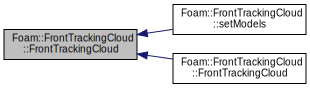
\includegraphics[width=350pt]{classFoam_1_1FrontTrackingCloud_ae9da3f76099b9b82be67cf99ae64ab28_icgraph}
\end{center}
\end{figure}
\mbox{\Hypertarget{classFoam_1_1FrontTrackingCloud_ad185ad598e5280fdea20a85d8aff1e91}\label{classFoam_1_1FrontTrackingCloud_ad185ad598e5280fdea20a85d8aff1e91}} 
\index{Foam\+::\+Front\+Tracking\+Cloud@{Foam\+::\+Front\+Tracking\+Cloud}!Front\+Tracking\+Cloud@{Front\+Tracking\+Cloud}}
\index{Front\+Tracking\+Cloud@{Front\+Tracking\+Cloud}!Foam\+::\+Front\+Tracking\+Cloud@{Foam\+::\+Front\+Tracking\+Cloud}}
\subsubsection{\texorpdfstring{Front\+Tracking\+Cloud()}{FrontTrackingCloud()}\hspace{0.1cm}{\footnotesize\ttfamily [2/10]}}
{\footnotesize\ttfamily template$<$class Cloud\+Type $>$ \\
\hyperlink{classFoam_1_1FrontTrackingCloud}{Foam\+::\+Front\+Tracking\+Cloud}$<$ Cloud\+Type $>$\+::\hyperlink{classFoam_1_1FrontTrackingCloud}{Front\+Tracking\+Cloud} (\begin{DoxyParamCaption}\item[{const word \&}]{cloud\+Name,  }\item[{const vol\+Scalar\+Field \&}]{rho,  }\item[{const vol\+Vector\+Field \&}]{U,  }\item[{const dimensioned\+Vector \&}]{g,  }\item[{const fluid\+Thermo \&}]{carrier\+Thermo,  }\item[{const bool}]{read\+Fields = {\ttfamily true} }\end{DoxyParamCaption})}

Here is the call graph for this function\+:\nopagebreak
\begin{figure}[H]
\begin{center}
\leavevmode
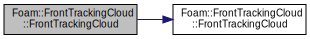
\includegraphics[width=350pt]{classFoam_1_1FrontTrackingCloud_ad185ad598e5280fdea20a85d8aff1e91_cgraph}
\end{center}
\end{figure}
\mbox{\Hypertarget{classFoam_1_1FrontTrackingCloud_aaf498c2097937a9147685bd0de6a85bb}\label{classFoam_1_1FrontTrackingCloud_aaf498c2097937a9147685bd0de6a85bb}} 
\index{Foam\+::\+Front\+Tracking\+Cloud@{Foam\+::\+Front\+Tracking\+Cloud}!Front\+Tracking\+Cloud@{Front\+Tracking\+Cloud}}
\index{Front\+Tracking\+Cloud@{Front\+Tracking\+Cloud}!Foam\+::\+Front\+Tracking\+Cloud@{Foam\+::\+Front\+Tracking\+Cloud}}
\subsubsection{\texorpdfstring{Front\+Tracking\+Cloud()}{FrontTrackingCloud()}\hspace{0.1cm}{\footnotesize\ttfamily [3/10]}}
{\footnotesize\ttfamily template$<$class Cloud\+Type $>$ \\
\hyperlink{classFoam_1_1FrontTrackingCloud}{Foam\+::\+Front\+Tracking\+Cloud}$<$ Cloud\+Type $>$\+::\hyperlink{classFoam_1_1FrontTrackingCloud}{Front\+Tracking\+Cloud} (\begin{DoxyParamCaption}\item[{\hyperlink{classFoam_1_1FrontTrackingCloud}{Front\+Tracking\+Cloud}$<$ Cloud\+Type $>$ \&}]{c,  }\item[{const word \&}]{name }\end{DoxyParamCaption})}

Here is the call graph for this function\+:\nopagebreak
\begin{figure}[H]
\begin{center}
\leavevmode
\includegraphics[width=350pt]{classFoam_1_1FrontTrackingCloud_aaf498c2097937a9147685bd0de6a85bb_cgraph}
\end{center}
\end{figure}
\mbox{\Hypertarget{classFoam_1_1FrontTrackingCloud_a87899dfd5f7408b0da887eafe1fb2a43}\label{classFoam_1_1FrontTrackingCloud_a87899dfd5f7408b0da887eafe1fb2a43}} 
\index{Foam\+::\+Front\+Tracking\+Cloud@{Foam\+::\+Front\+Tracking\+Cloud}!Front\+Tracking\+Cloud@{Front\+Tracking\+Cloud}}
\index{Front\+Tracking\+Cloud@{Front\+Tracking\+Cloud}!Foam\+::\+Front\+Tracking\+Cloud@{Foam\+::\+Front\+Tracking\+Cloud}}
\subsubsection{\texorpdfstring{Front\+Tracking\+Cloud()}{FrontTrackingCloud()}\hspace{0.1cm}{\footnotesize\ttfamily [4/10]}}
{\footnotesize\ttfamily template$<$class Cloud\+Type $>$ \\
\hyperlink{classFoam_1_1FrontTrackingCloud}{Foam\+::\+Front\+Tracking\+Cloud}$<$ Cloud\+Type $>$\+::\hyperlink{classFoam_1_1FrontTrackingCloud}{Front\+Tracking\+Cloud} (\begin{DoxyParamCaption}\item[{const fv\+Mesh \&}]{mesh,  }\item[{const word \&}]{name,  }\item[{const \hyperlink{classFoam_1_1FrontTrackingCloud}{Front\+Tracking\+Cloud}$<$ Cloud\+Type $>$ \&}]{c }\end{DoxyParamCaption})}

\mbox{\Hypertarget{classFoam_1_1FrontTrackingCloud_ac8860f6c62a4086d2cc0d00e28ed88de}\label{classFoam_1_1FrontTrackingCloud_ac8860f6c62a4086d2cc0d00e28ed88de}} 
\index{Foam\+::\+Front\+Tracking\+Cloud@{Foam\+::\+Front\+Tracking\+Cloud}!Front\+Tracking\+Cloud@{Front\+Tracking\+Cloud}}
\index{Front\+Tracking\+Cloud@{Front\+Tracking\+Cloud}!Foam\+::\+Front\+Tracking\+Cloud@{Foam\+::\+Front\+Tracking\+Cloud}}
\subsubsection{\texorpdfstring{Front\+Tracking\+Cloud()}{FrontTrackingCloud()}\hspace{0.1cm}{\footnotesize\ttfamily [5/10]}}
{\footnotesize\ttfamily template$<$class Cloud\+Type$>$ \\
\hyperlink{classFoam_1_1FrontTrackingCloud}{Foam\+::\+Front\+Tracking\+Cloud}$<$ Cloud\+Type $>$\+::\hyperlink{classFoam_1_1FrontTrackingCloud}{Front\+Tracking\+Cloud} (\begin{DoxyParamCaption}\item[{const \hyperlink{classFoam_1_1FrontTrackingCloud}{Front\+Tracking\+Cloud}$<$ Cloud\+Type $>$ \&}]{ }\end{DoxyParamCaption})\hspace{0.3cm}{\ttfamily [delete]}}

\mbox{\Hypertarget{classFoam_1_1FrontTrackingCloud_a8aaede4a1c43afed7a499fdbe20ba62a}\label{classFoam_1_1FrontTrackingCloud_a8aaede4a1c43afed7a499fdbe20ba62a}} 
\index{Foam\+::\+Front\+Tracking\+Cloud@{Foam\+::\+Front\+Tracking\+Cloud}!````~Front\+Tracking\+Cloud@{$\sim$\+Front\+Tracking\+Cloud}}
\index{````~Front\+Tracking\+Cloud@{$\sim$\+Front\+Tracking\+Cloud}!Foam\+::\+Front\+Tracking\+Cloud@{Foam\+::\+Front\+Tracking\+Cloud}}
\subsubsection{\texorpdfstring{$\sim$\+Front\+Tracking\+Cloud()}{~FrontTrackingCloud()}\hspace{0.1cm}{\footnotesize\ttfamily [1/2]}}
{\footnotesize\ttfamily template$<$class Cloud\+Type $>$ \\
\hyperlink{classFoam_1_1FrontTrackingCloud}{Foam\+::\+Front\+Tracking\+Cloud}$<$ Cloud\+Type $>$\+::$\sim$\hyperlink{classFoam_1_1FrontTrackingCloud}{Front\+Tracking\+Cloud} (\begin{DoxyParamCaption}{ }\end{DoxyParamCaption})\hspace{0.3cm}{\ttfamily [virtual]}}

\mbox{\Hypertarget{classFoam_1_1FrontTrackingCloud_ae9da3f76099b9b82be67cf99ae64ab28}\label{classFoam_1_1FrontTrackingCloud_ae9da3f76099b9b82be67cf99ae64ab28}} 
\index{Foam\+::\+Front\+Tracking\+Cloud@{Foam\+::\+Front\+Tracking\+Cloud}!Front\+Tracking\+Cloud@{Front\+Tracking\+Cloud}}
\index{Front\+Tracking\+Cloud@{Front\+Tracking\+Cloud}!Foam\+::\+Front\+Tracking\+Cloud@{Foam\+::\+Front\+Tracking\+Cloud}}
\subsubsection{\texorpdfstring{Front\+Tracking\+Cloud()}{FrontTrackingCloud()}\hspace{0.1cm}{\footnotesize\ttfamily [6/10]}}
{\footnotesize\ttfamily template$<$class Cloud\+Type$>$ \\
\hyperlink{classFoam_1_1FrontTrackingCloud}{Foam\+::\+Front\+Tracking\+Cloud}$<$ Cloud\+Type $>$\+::\hyperlink{classFoam_1_1FrontTrackingCloud}{Front\+Tracking\+Cloud} (\begin{DoxyParamCaption}\item[{const word \&}]{cloud\+Name,  }\item[{const vol\+Scalar\+Field \&}]{rho,  }\item[{const vol\+Vector\+Field \&}]{U,  }\item[{const vol\+Scalar\+Field \&}]{mu,  }\item[{const dimensioned\+Vector \&}]{g,  }\item[{const bool}]{read\+Fields = {\ttfamily true} }\end{DoxyParamCaption})}

\mbox{\Hypertarget{classFoam_1_1FrontTrackingCloud_ad185ad598e5280fdea20a85d8aff1e91}\label{classFoam_1_1FrontTrackingCloud_ad185ad598e5280fdea20a85d8aff1e91}} 
\index{Foam\+::\+Front\+Tracking\+Cloud@{Foam\+::\+Front\+Tracking\+Cloud}!Front\+Tracking\+Cloud@{Front\+Tracking\+Cloud}}
\index{Front\+Tracking\+Cloud@{Front\+Tracking\+Cloud}!Foam\+::\+Front\+Tracking\+Cloud@{Foam\+::\+Front\+Tracking\+Cloud}}
\subsubsection{\texorpdfstring{Front\+Tracking\+Cloud()}{FrontTrackingCloud()}\hspace{0.1cm}{\footnotesize\ttfamily [7/10]}}
{\footnotesize\ttfamily template$<$class Cloud\+Type$>$ \\
\hyperlink{classFoam_1_1FrontTrackingCloud}{Foam\+::\+Front\+Tracking\+Cloud}$<$ Cloud\+Type $>$\+::\hyperlink{classFoam_1_1FrontTrackingCloud}{Front\+Tracking\+Cloud} (\begin{DoxyParamCaption}\item[{const word \&}]{cloud\+Name,  }\item[{const vol\+Scalar\+Field \&}]{rho,  }\item[{const vol\+Vector\+Field \&}]{U,  }\item[{const dimensioned\+Vector \&}]{g,  }\item[{const fluid\+Thermo \&}]{carrier\+Thermo,  }\item[{const bool}]{read\+Fields = {\ttfamily true} }\end{DoxyParamCaption})}

\mbox{\Hypertarget{classFoam_1_1FrontTrackingCloud_aaf498c2097937a9147685bd0de6a85bb}\label{classFoam_1_1FrontTrackingCloud_aaf498c2097937a9147685bd0de6a85bb}} 
\index{Foam\+::\+Front\+Tracking\+Cloud@{Foam\+::\+Front\+Tracking\+Cloud}!Front\+Tracking\+Cloud@{Front\+Tracking\+Cloud}}
\index{Front\+Tracking\+Cloud@{Front\+Tracking\+Cloud}!Foam\+::\+Front\+Tracking\+Cloud@{Foam\+::\+Front\+Tracking\+Cloud}}
\subsubsection{\texorpdfstring{Front\+Tracking\+Cloud()}{FrontTrackingCloud()}\hspace{0.1cm}{\footnotesize\ttfamily [8/10]}}
{\footnotesize\ttfamily template$<$class Cloud\+Type$>$ \\
\hyperlink{classFoam_1_1FrontTrackingCloud}{Foam\+::\+Front\+Tracking\+Cloud}$<$ Cloud\+Type $>$\+::\hyperlink{classFoam_1_1FrontTrackingCloud}{Front\+Tracking\+Cloud} (\begin{DoxyParamCaption}\item[{\hyperlink{classFoam_1_1FrontTrackingCloud}{Front\+Tracking\+Cloud}$<$ Cloud\+Type $>$ \&}]{c,  }\item[{const word \&}]{name }\end{DoxyParamCaption})}

\mbox{\Hypertarget{classFoam_1_1FrontTrackingCloud_a87899dfd5f7408b0da887eafe1fb2a43}\label{classFoam_1_1FrontTrackingCloud_a87899dfd5f7408b0da887eafe1fb2a43}} 
\index{Foam\+::\+Front\+Tracking\+Cloud@{Foam\+::\+Front\+Tracking\+Cloud}!Front\+Tracking\+Cloud@{Front\+Tracking\+Cloud}}
\index{Front\+Tracking\+Cloud@{Front\+Tracking\+Cloud}!Foam\+::\+Front\+Tracking\+Cloud@{Foam\+::\+Front\+Tracking\+Cloud}}
\subsubsection{\texorpdfstring{Front\+Tracking\+Cloud()}{FrontTrackingCloud()}\hspace{0.1cm}{\footnotesize\ttfamily [9/10]}}
{\footnotesize\ttfamily template$<$class Cloud\+Type$>$ \\
\hyperlink{classFoam_1_1FrontTrackingCloud}{Foam\+::\+Front\+Tracking\+Cloud}$<$ Cloud\+Type $>$\+::\hyperlink{classFoam_1_1FrontTrackingCloud}{Front\+Tracking\+Cloud} (\begin{DoxyParamCaption}\item[{const fv\+Mesh \&}]{mesh,  }\item[{const word \&}]{name,  }\item[{const \hyperlink{classFoam_1_1FrontTrackingCloud}{Front\+Tracking\+Cloud}$<$ Cloud\+Type $>$ \&}]{c }\end{DoxyParamCaption})}

\mbox{\Hypertarget{classFoam_1_1FrontTrackingCloud_ac8860f6c62a4086d2cc0d00e28ed88de}\label{classFoam_1_1FrontTrackingCloud_ac8860f6c62a4086d2cc0d00e28ed88de}} 
\index{Foam\+::\+Front\+Tracking\+Cloud@{Foam\+::\+Front\+Tracking\+Cloud}!Front\+Tracking\+Cloud@{Front\+Tracking\+Cloud}}
\index{Front\+Tracking\+Cloud@{Front\+Tracking\+Cloud}!Foam\+::\+Front\+Tracking\+Cloud@{Foam\+::\+Front\+Tracking\+Cloud}}
\subsubsection{\texorpdfstring{Front\+Tracking\+Cloud()}{FrontTrackingCloud()}\hspace{0.1cm}{\footnotesize\ttfamily [10/10]}}
{\footnotesize\ttfamily template$<$class Cloud\+Type$>$ \\
\hyperlink{classFoam_1_1FrontTrackingCloud}{Foam\+::\+Front\+Tracking\+Cloud}$<$ Cloud\+Type $>$\+::\hyperlink{classFoam_1_1FrontTrackingCloud}{Front\+Tracking\+Cloud} (\begin{DoxyParamCaption}\item[{const \hyperlink{classFoam_1_1FrontTrackingCloud}{Front\+Tracking\+Cloud}$<$ Cloud\+Type $>$ \&}]{ }\end{DoxyParamCaption})\hspace{0.3cm}{\ttfamily [delete]}}

\mbox{\Hypertarget{classFoam_1_1FrontTrackingCloud_adcba24981e24cd97517d109b4197d2c8}\label{classFoam_1_1FrontTrackingCloud_adcba24981e24cd97517d109b4197d2c8}} 
\index{Foam\+::\+Front\+Tracking\+Cloud@{Foam\+::\+Front\+Tracking\+Cloud}!````~Front\+Tracking\+Cloud@{$\sim$\+Front\+Tracking\+Cloud}}
\index{````~Front\+Tracking\+Cloud@{$\sim$\+Front\+Tracking\+Cloud}!Foam\+::\+Front\+Tracking\+Cloud@{Foam\+::\+Front\+Tracking\+Cloud}}
\subsubsection{\texorpdfstring{$\sim$\+Front\+Tracking\+Cloud()}{~FrontTrackingCloud()}\hspace{0.1cm}{\footnotesize\ttfamily [2/2]}}
{\footnotesize\ttfamily template$<$class Cloud\+Type$>$ \\
virtual \hyperlink{classFoam_1_1FrontTrackingCloud}{Foam\+::\+Front\+Tracking\+Cloud}$<$ Cloud\+Type $>$\+::$\sim$\hyperlink{classFoam_1_1FrontTrackingCloud}{Front\+Tracking\+Cloud} (\begin{DoxyParamCaption}{ }\end{DoxyParamCaption})\hspace{0.3cm}{\ttfamily [virtual]}}



\subsection{Member Function Documentation}
\mbox{\Hypertarget{classFoam_1_1FrontTrackingCloud_ada5f5e05db21f49b7d61c74fecc37db0}\label{classFoam_1_1FrontTrackingCloud_ada5f5e05db21f49b7d61c74fecc37db0}} 
\index{Foam\+::\+Front\+Tracking\+Cloud@{Foam\+::\+Front\+Tracking\+Cloud}!adjusting\+The\+Cloud\+Data\+After\+Changes@{adjusting\+The\+Cloud\+Data\+After\+Changes}}
\index{adjusting\+The\+Cloud\+Data\+After\+Changes@{adjusting\+The\+Cloud\+Data\+After\+Changes}!Foam\+::\+Front\+Tracking\+Cloud@{Foam\+::\+Front\+Tracking\+Cloud}}
\subsubsection{\texorpdfstring{adjusting\+The\+Cloud\+Data\+After\+Changes()}{adjustingTheCloudDataAfterChanges()}\hspace{0.1cm}{\footnotesize\ttfamily [1/2]}}
{\footnotesize\ttfamily template$<$class Cloud\+Type $>$ \\
void \hyperlink{classFoam_1_1FrontTrackingCloud}{Foam\+::\+Front\+Tracking\+Cloud}$<$ Cloud\+Type $>$\+::adjusting\+The\+Cloud\+Data\+After\+Changes (\begin{DoxyParamCaption}\item[{label\+List \&}]{loc\+In\+Point\+Data\+List,  }\item[{label}]{b\+DI }\end{DoxyParamCaption})}

Here is the call graph for this function\+:\nopagebreak
\begin{figure}[H]
\begin{center}
\leavevmode
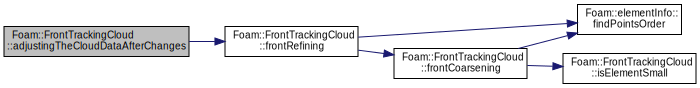
\includegraphics[width=350pt]{classFoam_1_1FrontTrackingCloud_ada5f5e05db21f49b7d61c74fecc37db0_cgraph}
\end{center}
\end{figure}
Here is the caller graph for this function\+:\nopagebreak
\begin{figure}[H]
\begin{center}
\leavevmode
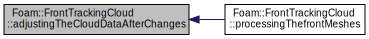
\includegraphics[width=350pt]{classFoam_1_1FrontTrackingCloud_ada5f5e05db21f49b7d61c74fecc37db0_icgraph}
\end{center}
\end{figure}
\mbox{\Hypertarget{classFoam_1_1FrontTrackingCloud_ada5f5e05db21f49b7d61c74fecc37db0}\label{classFoam_1_1FrontTrackingCloud_ada5f5e05db21f49b7d61c74fecc37db0}} 
\index{Foam\+::\+Front\+Tracking\+Cloud@{Foam\+::\+Front\+Tracking\+Cloud}!adjusting\+The\+Cloud\+Data\+After\+Changes@{adjusting\+The\+Cloud\+Data\+After\+Changes}}
\index{adjusting\+The\+Cloud\+Data\+After\+Changes@{adjusting\+The\+Cloud\+Data\+After\+Changes}!Foam\+::\+Front\+Tracking\+Cloud@{Foam\+::\+Front\+Tracking\+Cloud}}
\subsubsection{\texorpdfstring{adjusting\+The\+Cloud\+Data\+After\+Changes()}{adjustingTheCloudDataAfterChanges()}\hspace{0.1cm}{\footnotesize\ttfamily [2/2]}}
{\footnotesize\ttfamily template$<$class Cloud\+Type$>$ \\
void \hyperlink{classFoam_1_1FrontTrackingCloud}{Foam\+::\+Front\+Tracking\+Cloud}$<$ Cloud\+Type $>$\+::adjusting\+The\+Cloud\+Data\+After\+Changes (\begin{DoxyParamCaption}\item[{label\+List \&}]{loc\+In\+Point\+Data\+List,  }\item[{label}]{b\+DI }\end{DoxyParamCaption})}

\mbox{\Hypertarget{classFoam_1_1FrontTrackingCloud_a3cc5fbc7520219ddd33f6bc589722b82}\label{classFoam_1_1FrontTrackingCloud_a3cc5fbc7520219ddd33f6bc589722b82}} 
\index{Foam\+::\+Front\+Tracking\+Cloud@{Foam\+::\+Front\+Tracking\+Cloud}!all\+Cells\+In\+Eeach\+Masket@{all\+Cells\+In\+Eeach\+Masket}}
\index{all\+Cells\+In\+Eeach\+Masket@{all\+Cells\+In\+Eeach\+Masket}!Foam\+::\+Front\+Tracking\+Cloud@{Foam\+::\+Front\+Tracking\+Cloud}}
\subsubsection{\texorpdfstring{all\+Cells\+In\+Eeach\+Masket()}{allCellsInEeachMasket()}\hspace{0.1cm}{\footnotesize\ttfamily [1/2]}}
{\footnotesize\ttfamily template$<$class Cloud\+Type $>$ \\
Foam\+::\+List$<$ Dynamic\+List$<$ label $>$ $>$ \hyperlink{classFoam_1_1FrontTrackingCloud}{Foam\+::\+Front\+Tracking\+Cloud}$<$ Cloud\+Type $>$\+::all\+Cells\+In\+Eeach\+Masket (\begin{DoxyParamCaption}{ }\end{DoxyParamCaption}) const\hspace{0.3cm}{\ttfamily [inline]}}

\mbox{\Hypertarget{classFoam_1_1FrontTrackingCloud_a64fb8f2d5fe450ed751ec77733f12641}\label{classFoam_1_1FrontTrackingCloud_a64fb8f2d5fe450ed751ec77733f12641}} 
\index{Foam\+::\+Front\+Tracking\+Cloud@{Foam\+::\+Front\+Tracking\+Cloud}!all\+Cells\+In\+Eeach\+Masket@{all\+Cells\+In\+Eeach\+Masket}}
\index{all\+Cells\+In\+Eeach\+Masket@{all\+Cells\+In\+Eeach\+Masket}!Foam\+::\+Front\+Tracking\+Cloud@{Foam\+::\+Front\+Tracking\+Cloud}}
\subsubsection{\texorpdfstring{all\+Cells\+In\+Eeach\+Masket()}{allCellsInEeachMasket()}\hspace{0.1cm}{\footnotesize\ttfamily [2/2]}}
{\footnotesize\ttfamily template$<$class Cloud\+Type$>$ \\
List$<$Dynamic\+List$<$label$>$ $>$ \hyperlink{classFoam_1_1FrontTrackingCloud}{Foam\+::\+Front\+Tracking\+Cloud}$<$ Cloud\+Type $>$\+::all\+Cells\+In\+Eeach\+Masket (\begin{DoxyParamCaption}{ }\end{DoxyParamCaption}) const\hspace{0.3cm}{\ttfamily [inline]}}

\mbox{\Hypertarget{classFoam_1_1FrontTrackingCloud_a2facef866c2c46b20c00baf6e2836df8}\label{classFoam_1_1FrontTrackingCloud_a2facef866c2c46b20c00baf6e2836df8}} 
\index{Foam\+::\+Front\+Tracking\+Cloud@{Foam\+::\+Front\+Tracking\+Cloud}!b\+DataL@{b\+DataL}}
\index{b\+DataL@{b\+DataL}!Foam\+::\+Front\+Tracking\+Cloud@{Foam\+::\+Front\+Tracking\+Cloud}}
\subsubsection{\texorpdfstring{b\+Data\+L()}{bDataL()}\hspace{0.1cm}{\footnotesize\ttfamily [1/4]}}
{\footnotesize\ttfamily template$<$class Cloud\+Type $>$ \\
const Foam\+::\+Dynamic\+List$<$ \hyperlink{classFoam_1_1bubbleData}{bubble\+Data} $>$ \& \hyperlink{classFoam_1_1FrontTrackingCloud}{Foam\+::\+Front\+Tracking\+Cloud}$<$ Cloud\+Type $>$\+::b\+DataL (\begin{DoxyParamCaption}{ }\end{DoxyParamCaption}) const\hspace{0.3cm}{\ttfamily [inline]}}

\mbox{\Hypertarget{classFoam_1_1FrontTrackingCloud_aad777230d88c98be784780bbdd6ec4d8}\label{classFoam_1_1FrontTrackingCloud_aad777230d88c98be784780bbdd6ec4d8}} 
\index{Foam\+::\+Front\+Tracking\+Cloud@{Foam\+::\+Front\+Tracking\+Cloud}!b\+DataL@{b\+DataL}}
\index{b\+DataL@{b\+DataL}!Foam\+::\+Front\+Tracking\+Cloud@{Foam\+::\+Front\+Tracking\+Cloud}}
\subsubsection{\texorpdfstring{b\+Data\+L()}{bDataL()}\hspace{0.1cm}{\footnotesize\ttfamily [2/4]}}
{\footnotesize\ttfamily template$<$class Cloud\+Type$>$ \\
const Dynamic\+List$<$\hyperlink{classFoam_1_1bubbleData}{bubble\+Data}$>$\& \hyperlink{classFoam_1_1FrontTrackingCloud}{Foam\+::\+Front\+Tracking\+Cloud}$<$ Cloud\+Type $>$\+::b\+DataL (\begin{DoxyParamCaption}{ }\end{DoxyParamCaption}) const\hspace{0.3cm}{\ttfamily [inline]}}

\mbox{\Hypertarget{classFoam_1_1FrontTrackingCloud_ad609a644410a3223f9c6e089f491ad33}\label{classFoam_1_1FrontTrackingCloud_ad609a644410a3223f9c6e089f491ad33}} 
\index{Foam\+::\+Front\+Tracking\+Cloud@{Foam\+::\+Front\+Tracking\+Cloud}!b\+DataL@{b\+DataL}}
\index{b\+DataL@{b\+DataL}!Foam\+::\+Front\+Tracking\+Cloud@{Foam\+::\+Front\+Tracking\+Cloud}}
\subsubsection{\texorpdfstring{b\+Data\+L()}{bDataL()}\hspace{0.1cm}{\footnotesize\ttfamily [3/4]}}
{\footnotesize\ttfamily template$<$class Cloud\+Type $>$ \\
Foam\+::\+Dynamic\+List$<$ \hyperlink{classFoam_1_1bubbleData}{bubble\+Data} $>$ \& \hyperlink{classFoam_1_1FrontTrackingCloud}{Foam\+::\+Front\+Tracking\+Cloud}$<$ Cloud\+Type $>$\+::b\+DataL (\begin{DoxyParamCaption}{ }\end{DoxyParamCaption})\hspace{0.3cm}{\ttfamily [inline]}}

\mbox{\Hypertarget{classFoam_1_1FrontTrackingCloud_af54f24334180fe52e27dce8b1496403c}\label{classFoam_1_1FrontTrackingCloud_af54f24334180fe52e27dce8b1496403c}} 
\index{Foam\+::\+Front\+Tracking\+Cloud@{Foam\+::\+Front\+Tracking\+Cloud}!b\+DataL@{b\+DataL}}
\index{b\+DataL@{b\+DataL}!Foam\+::\+Front\+Tracking\+Cloud@{Foam\+::\+Front\+Tracking\+Cloud}}
\subsubsection{\texorpdfstring{b\+Data\+L()}{bDataL()}\hspace{0.1cm}{\footnotesize\ttfamily [4/4]}}
{\footnotesize\ttfamily template$<$class Cloud\+Type$>$ \\
Dynamic\+List$<$\hyperlink{classFoam_1_1bubbleData}{bubble\+Data}$>$\& \hyperlink{classFoam_1_1FrontTrackingCloud}{Foam\+::\+Front\+Tracking\+Cloud}$<$ Cloud\+Type $>$\+::b\+DataL (\begin{DoxyParamCaption}{ }\end{DoxyParamCaption})\hspace{0.3cm}{\ttfamily [inline]}}

\mbox{\Hypertarget{classFoam_1_1FrontTrackingCloud_a9d5d59f9f43a2a45c8788b0cc3e9ea0b}\label{classFoam_1_1FrontTrackingCloud_a9d5d59f9f43a2a45c8788b0cc3e9ea0b}} 
\index{Foam\+::\+Front\+Tracking\+Cloud@{Foam\+::\+Front\+Tracking\+Cloud}!bubble\+Post\+Processing@{bubble\+Post\+Processing}}
\index{bubble\+Post\+Processing@{bubble\+Post\+Processing}!Foam\+::\+Front\+Tracking\+Cloud@{Foam\+::\+Front\+Tracking\+Cloud}}
\subsubsection{\texorpdfstring{bubble\+Post\+Processing()}{bubblePostProcessing()}\hspace{0.1cm}{\footnotesize\ttfamily [1/2]}}
{\footnotesize\ttfamily template$<$class Cloud\+Type $>$ \\
void \hyperlink{classFoam_1_1FrontTrackingCloud}{Foam\+::\+Front\+Tracking\+Cloud}$<$ Cloud\+Type $>$\+::bubble\+Post\+Processing (\begin{DoxyParamCaption}{ }\end{DoxyParamCaption})}

\mbox{\Hypertarget{classFoam_1_1FrontTrackingCloud_a9d5d59f9f43a2a45c8788b0cc3e9ea0b}\label{classFoam_1_1FrontTrackingCloud_a9d5d59f9f43a2a45c8788b0cc3e9ea0b}} 
\index{Foam\+::\+Front\+Tracking\+Cloud@{Foam\+::\+Front\+Tracking\+Cloud}!bubble\+Post\+Processing@{bubble\+Post\+Processing}}
\index{bubble\+Post\+Processing@{bubble\+Post\+Processing}!Foam\+::\+Front\+Tracking\+Cloud@{Foam\+::\+Front\+Tracking\+Cloud}}
\subsubsection{\texorpdfstring{bubble\+Post\+Processing()}{bubblePostProcessing()}\hspace{0.1cm}{\footnotesize\ttfamily [2/2]}}
{\footnotesize\ttfamily template$<$class Cloud\+Type$>$ \\
void \hyperlink{classFoam_1_1FrontTrackingCloud}{Foam\+::\+Front\+Tracking\+Cloud}$<$ Cloud\+Type $>$\+::bubble\+Post\+Processing (\begin{DoxyParamCaption}{ }\end{DoxyParamCaption})}

\mbox{\Hypertarget{classFoam_1_1FrontTrackingCloud_a5637e3be2d96f505313e700e31d96d3f}\label{classFoam_1_1FrontTrackingCloud_a5637e3be2d96f505313e700e31d96d3f}} 
\index{Foam\+::\+Front\+Tracking\+Cloud@{Foam\+::\+Front\+Tracking\+Cloud}!calc\+Bubble\+Non\+Dimensional\+Numbers@{calc\+Bubble\+Non\+Dimensional\+Numbers}}
\index{calc\+Bubble\+Non\+Dimensional\+Numbers@{calc\+Bubble\+Non\+Dimensional\+Numbers}!Foam\+::\+Front\+Tracking\+Cloud@{Foam\+::\+Front\+Tracking\+Cloud}}
\subsubsection{\texorpdfstring{calc\+Bubble\+Non\+Dimensional\+Numbers()}{calcBubbleNonDimensionalNumbers()}\hspace{0.1cm}{\footnotesize\ttfamily [1/2]}}
{\footnotesize\ttfamily template$<$class Cloud\+Type $>$ \\
void \hyperlink{classFoam_1_1FrontTrackingCloud}{Foam\+::\+Front\+Tracking\+Cloud}$<$ Cloud\+Type $>$\+::calc\+Bubble\+Non\+Dimensional\+Numbers (\begin{DoxyParamCaption}{ }\end{DoxyParamCaption})\hspace{0.3cm}{\ttfamily [inline]}}

\mbox{\Hypertarget{classFoam_1_1FrontTrackingCloud_a5637e3be2d96f505313e700e31d96d3f}\label{classFoam_1_1FrontTrackingCloud_a5637e3be2d96f505313e700e31d96d3f}} 
\index{Foam\+::\+Front\+Tracking\+Cloud@{Foam\+::\+Front\+Tracking\+Cloud}!calc\+Bubble\+Non\+Dimensional\+Numbers@{calc\+Bubble\+Non\+Dimensional\+Numbers}}
\index{calc\+Bubble\+Non\+Dimensional\+Numbers@{calc\+Bubble\+Non\+Dimensional\+Numbers}!Foam\+::\+Front\+Tracking\+Cloud@{Foam\+::\+Front\+Tracking\+Cloud}}
\subsubsection{\texorpdfstring{calc\+Bubble\+Non\+Dimensional\+Numbers()}{calcBubbleNonDimensionalNumbers()}\hspace{0.1cm}{\footnotesize\ttfamily [2/2]}}
{\footnotesize\ttfamily template$<$class Cloud\+Type$>$ \\
void \hyperlink{classFoam_1_1FrontTrackingCloud}{Foam\+::\+Front\+Tracking\+Cloud}$<$ Cloud\+Type $>$\+::calc\+Bubble\+Non\+Dimensional\+Numbers (\begin{DoxyParamCaption}{ }\end{DoxyParamCaption})\hspace{0.3cm}{\ttfamily [inline]}}

\mbox{\Hypertarget{classFoam_1_1FrontTrackingCloud_aa8d4bc5e201416b5b147c184c11940df}\label{classFoam_1_1FrontTrackingCloud_aa8d4bc5e201416b5b147c184c11940df}} 
\index{Foam\+::\+Front\+Tracking\+Cloud@{Foam\+::\+Front\+Tracking\+Cloud}!calc\+Length\+Scale\+Of\+The\+Mesh@{calc\+Length\+Scale\+Of\+The\+Mesh}}
\index{calc\+Length\+Scale\+Of\+The\+Mesh@{calc\+Length\+Scale\+Of\+The\+Mesh}!Foam\+::\+Front\+Tracking\+Cloud@{Foam\+::\+Front\+Tracking\+Cloud}}
\subsubsection{\texorpdfstring{calc\+Length\+Scale\+Of\+The\+Mesh()}{calcLengthScaleOfTheMesh()}\hspace{0.1cm}{\footnotesize\ttfamily [1/2]}}
{\footnotesize\ttfamily template$<$class Cloud\+Type $>$ \\
Foam\+::scalar \hyperlink{classFoam_1_1FrontTrackingCloud}{Foam\+::\+Front\+Tracking\+Cloud}$<$ Cloud\+Type $>$\+::calc\+Length\+Scale\+Of\+The\+Mesh (\begin{DoxyParamCaption}{ }\end{DoxyParamCaption})\hspace{0.3cm}{\ttfamily [inline]}}

\mbox{\Hypertarget{classFoam_1_1FrontTrackingCloud_aa8d4bc5e201416b5b147c184c11940df}\label{classFoam_1_1FrontTrackingCloud_aa8d4bc5e201416b5b147c184c11940df}} 
\index{Foam\+::\+Front\+Tracking\+Cloud@{Foam\+::\+Front\+Tracking\+Cloud}!calc\+Length\+Scale\+Of\+The\+Mesh@{calc\+Length\+Scale\+Of\+The\+Mesh}}
\index{calc\+Length\+Scale\+Of\+The\+Mesh@{calc\+Length\+Scale\+Of\+The\+Mesh}!Foam\+::\+Front\+Tracking\+Cloud@{Foam\+::\+Front\+Tracking\+Cloud}}
\subsubsection{\texorpdfstring{calc\+Length\+Scale\+Of\+The\+Mesh()}{calcLengthScaleOfTheMesh()}\hspace{0.1cm}{\footnotesize\ttfamily [2/2]}}
{\footnotesize\ttfamily template$<$class Cloud\+Type$>$ \\
Foam\+::scalar \hyperlink{classFoam_1_1FrontTrackingCloud}{Foam\+::\+Front\+Tracking\+Cloud}$<$ Cloud\+Type $>$\+::calc\+Length\+Scale\+Of\+The\+Mesh (\begin{DoxyParamCaption}{ }\end{DoxyParamCaption})\hspace{0.3cm}{\ttfamily [inline]}}

\mbox{\Hypertarget{classFoam_1_1FrontTrackingCloud_ad82d33465c7a25d3d72f5ec29707edd4}\label{classFoam_1_1FrontTrackingCloud_ad82d33465c7a25d3d72f5ec29707edd4}} 
\index{Foam\+::\+Front\+Tracking\+Cloud@{Foam\+::\+Front\+Tracking\+Cloud}!clone@{clone}}
\index{clone@{clone}!Foam\+::\+Front\+Tracking\+Cloud@{Foam\+::\+Front\+Tracking\+Cloud}}
\subsubsection{\texorpdfstring{clone()}{clone()}\hspace{0.1cm}{\footnotesize\ttfamily [1/2]}}
{\footnotesize\ttfamily template$<$class Cloud\+Type$>$ \\
virtual auto\+Ptr$<$Cloud$<$\hyperlink{classFoam_1_1FrontTrackingCloud_a18be05626026eec2bf2a990da073a350}{parcel\+Type}$>$ $>$ \hyperlink{classFoam_1_1FrontTrackingCloud}{Foam\+::\+Front\+Tracking\+Cloud}$<$ Cloud\+Type $>$\+::clone (\begin{DoxyParamCaption}\item[{const word \&}]{name }\end{DoxyParamCaption})\hspace{0.3cm}{\ttfamily [inline]}, {\ttfamily [virtual]}}

\mbox{\Hypertarget{classFoam_1_1FrontTrackingCloud_ad82d33465c7a25d3d72f5ec29707edd4}\label{classFoam_1_1FrontTrackingCloud_ad82d33465c7a25d3d72f5ec29707edd4}} 
\index{Foam\+::\+Front\+Tracking\+Cloud@{Foam\+::\+Front\+Tracking\+Cloud}!clone@{clone}}
\index{clone@{clone}!Foam\+::\+Front\+Tracking\+Cloud@{Foam\+::\+Front\+Tracking\+Cloud}}
\subsubsection{\texorpdfstring{clone()}{clone()}\hspace{0.1cm}{\footnotesize\ttfamily [2/2]}}
{\footnotesize\ttfamily template$<$class Cloud\+Type$>$ \\
virtual auto\+Ptr$<$Cloud$<$\hyperlink{classFoam_1_1FrontTrackingCloud_a18be05626026eec2bf2a990da073a350}{parcel\+Type}$>$ $>$ \hyperlink{classFoam_1_1FrontTrackingCloud}{Foam\+::\+Front\+Tracking\+Cloud}$<$ Cloud\+Type $>$\+::clone (\begin{DoxyParamCaption}\item[{const word \&}]{name }\end{DoxyParamCaption})\hspace{0.3cm}{\ttfamily [inline]}, {\ttfamily [virtual]}}

\mbox{\Hypertarget{classFoam_1_1FrontTrackingCloud_aaee595291402fafdae131c72fe7c8a38}\label{classFoam_1_1FrontTrackingCloud_aaee595291402fafdae131c72fe7c8a38}} 
\index{Foam\+::\+Front\+Tracking\+Cloud@{Foam\+::\+Front\+Tracking\+Cloud}!clone\+Bare@{clone\+Bare}}
\index{clone\+Bare@{clone\+Bare}!Foam\+::\+Front\+Tracking\+Cloud@{Foam\+::\+Front\+Tracking\+Cloud}}
\subsubsection{\texorpdfstring{clone\+Bare()}{cloneBare()}\hspace{0.1cm}{\footnotesize\ttfamily [1/2]}}
{\footnotesize\ttfamily template$<$class Cloud\+Type$>$ \\
virtual auto\+Ptr$<$Cloud$<$\hyperlink{classFoam_1_1FrontTrackingCloud_a18be05626026eec2bf2a990da073a350}{parcel\+Type}$>$ $>$ \hyperlink{classFoam_1_1FrontTrackingCloud}{Foam\+::\+Front\+Tracking\+Cloud}$<$ Cloud\+Type $>$\+::clone\+Bare (\begin{DoxyParamCaption}\item[{const word \&}]{name }\end{DoxyParamCaption}) const\hspace{0.3cm}{\ttfamily [inline]}, {\ttfamily [virtual]}}

\mbox{\Hypertarget{classFoam_1_1FrontTrackingCloud_aaee595291402fafdae131c72fe7c8a38}\label{classFoam_1_1FrontTrackingCloud_aaee595291402fafdae131c72fe7c8a38}} 
\index{Foam\+::\+Front\+Tracking\+Cloud@{Foam\+::\+Front\+Tracking\+Cloud}!clone\+Bare@{clone\+Bare}}
\index{clone\+Bare@{clone\+Bare}!Foam\+::\+Front\+Tracking\+Cloud@{Foam\+::\+Front\+Tracking\+Cloud}}
\subsubsection{\texorpdfstring{clone\+Bare()}{cloneBare()}\hspace{0.1cm}{\footnotesize\ttfamily [2/2]}}
{\footnotesize\ttfamily template$<$class Cloud\+Type$>$ \\
virtual auto\+Ptr$<$Cloud$<$\hyperlink{classFoam_1_1FrontTrackingCloud_a18be05626026eec2bf2a990da073a350}{parcel\+Type}$>$ $>$ \hyperlink{classFoam_1_1FrontTrackingCloud}{Foam\+::\+Front\+Tracking\+Cloud}$<$ Cloud\+Type $>$\+::clone\+Bare (\begin{DoxyParamCaption}\item[{const word \&}]{name }\end{DoxyParamCaption}) const\hspace{0.3cm}{\ttfamily [inline]}, {\ttfamily [virtual]}}

\mbox{\Hypertarget{classFoam_1_1FrontTrackingCloud_ab56e418175f86982ef3b36c6e74e4fdc}\label{classFoam_1_1FrontTrackingCloud_ab56e418175f86982ef3b36c6e74e4fdc}} 
\index{Foam\+::\+Front\+Tracking\+Cloud@{Foam\+::\+Front\+Tracking\+Cloud}!cloud\+Cleaning@{cloud\+Cleaning}}
\index{cloud\+Cleaning@{cloud\+Cleaning}!Foam\+::\+Front\+Tracking\+Cloud@{Foam\+::\+Front\+Tracking\+Cloud}}
\subsubsection{\texorpdfstring{cloud\+Cleaning()}{cloudCleaning()}\hspace{0.1cm}{\footnotesize\ttfamily [1/2]}}
{\footnotesize\ttfamily template$<$class Cloud\+Type$>$ \\
void \hyperlink{classFoam_1_1FrontTrackingCloud}{Foam\+::\+Front\+Tracking\+Cloud}$<$ Cloud\+Type $>$\+::cloud\+Cleaning (\begin{DoxyParamCaption}{ }\end{DoxyParamCaption})}

\mbox{\Hypertarget{classFoam_1_1FrontTrackingCloud_ab56e418175f86982ef3b36c6e74e4fdc}\label{classFoam_1_1FrontTrackingCloud_ab56e418175f86982ef3b36c6e74e4fdc}} 
\index{Foam\+::\+Front\+Tracking\+Cloud@{Foam\+::\+Front\+Tracking\+Cloud}!cloud\+Cleaning@{cloud\+Cleaning}}
\index{cloud\+Cleaning@{cloud\+Cleaning}!Foam\+::\+Front\+Tracking\+Cloud@{Foam\+::\+Front\+Tracking\+Cloud}}
\subsubsection{\texorpdfstring{cloud\+Cleaning()}{cloudCleaning()}\hspace{0.1cm}{\footnotesize\ttfamily [2/2]}}
{\footnotesize\ttfamily template$<$class Cloud\+Type $>$ \\
void \hyperlink{classFoam_1_1FrontTrackingCloud}{Foam\+::\+Front\+Tracking\+Cloud}$<$ Cloud\+Type $>$\+::cloud\+Cleaning (\begin{DoxyParamCaption}{ }\end{DoxyParamCaption})}

\mbox{\Hypertarget{classFoam_1_1FrontTrackingCloud_a916ec076f5dac6164f4908e49759d5d3}\label{classFoam_1_1FrontTrackingCloud_a916ec076f5dac6164f4908e49759d5d3}} 
\index{Foam\+::\+Front\+Tracking\+Cloud@{Foam\+::\+Front\+Tracking\+Cloud}!cloud\+Copy@{cloud\+Copy}}
\index{cloud\+Copy@{cloud\+Copy}!Foam\+::\+Front\+Tracking\+Cloud@{Foam\+::\+Front\+Tracking\+Cloud}}
\subsubsection{\texorpdfstring{cloud\+Copy()}{cloudCopy()}\hspace{0.1cm}{\footnotesize\ttfamily [1/2]}}
{\footnotesize\ttfamily template$<$class Cloud\+Type$>$ \\
const \hyperlink{classFoam_1_1FrontTrackingCloud}{Front\+Tracking\+Cloud}\& \hyperlink{classFoam_1_1FrontTrackingCloud}{Foam\+::\+Front\+Tracking\+Cloud}$<$ Cloud\+Type $>$\+::cloud\+Copy (\begin{DoxyParamCaption}{ }\end{DoxyParamCaption}) const\hspace{0.3cm}{\ttfamily [inline]}}

\mbox{\Hypertarget{classFoam_1_1FrontTrackingCloud_a5de0cfc162d5fca7f01c09bec6484a80}\label{classFoam_1_1FrontTrackingCloud_a5de0cfc162d5fca7f01c09bec6484a80}} 
\index{Foam\+::\+Front\+Tracking\+Cloud@{Foam\+::\+Front\+Tracking\+Cloud}!cloud\+Copy@{cloud\+Copy}}
\index{cloud\+Copy@{cloud\+Copy}!Foam\+::\+Front\+Tracking\+Cloud@{Foam\+::\+Front\+Tracking\+Cloud}}
\subsubsection{\texorpdfstring{cloud\+Copy()}{cloudCopy()}\hspace{0.1cm}{\footnotesize\ttfamily [2/2]}}
{\footnotesize\ttfamily template$<$class Cloud\+Type $>$ \\
const \hyperlink{classFoam_1_1FrontTrackingCloud}{Foam\+::\+Front\+Tracking\+Cloud}$<$ Cloud\+Type $>$ \& \hyperlink{classFoam_1_1FrontTrackingCloud}{Foam\+::\+Front\+Tracking\+Cloud}$<$ Cloud\+Type $>$\+::cloud\+Copy (\begin{DoxyParamCaption}{ }\end{DoxyParamCaption}) const\hspace{0.3cm}{\ttfamily [inline]}}

Here is the call graph for this function\+:\nopagebreak
\begin{figure}[H]
\begin{center}
\leavevmode
\includegraphics[width=350pt]{classFoam_1_1FrontTrackingCloud_a5de0cfc162d5fca7f01c09bec6484a80_cgraph}
\end{center}
\end{figure}
\mbox{\Hypertarget{classFoam_1_1FrontTrackingCloud_ab7706a4a237ef93320cf8194480a4847}\label{classFoam_1_1FrontTrackingCloud_ab7706a4a237ef93320cf8194480a4847}} 
\index{Foam\+::\+Front\+Tracking\+Cloud@{Foam\+::\+Front\+Tracking\+Cloud}!communications\+Of\+The\+Front\+And\+Eulerian\+Grid@{communications\+Of\+The\+Front\+And\+Eulerian\+Grid}}
\index{communications\+Of\+The\+Front\+And\+Eulerian\+Grid@{communications\+Of\+The\+Front\+And\+Eulerian\+Grid}!Foam\+::\+Front\+Tracking\+Cloud@{Foam\+::\+Front\+Tracking\+Cloud}}
\subsubsection{\texorpdfstring{communications\+Of\+The\+Front\+And\+Eulerian\+Grid()}{communicationsOfTheFrontAndEulerianGrid()}\hspace{0.1cm}{\footnotesize\ttfamily [1/2]}}
{\footnotesize\ttfamily template$<$class Cloud\+Type $>$ \\
void \hyperlink{classFoam_1_1FrontTrackingCloud}{Foam\+::\+Front\+Tracking\+Cloud}$<$ Cloud\+Type $>$\+::communications\+Of\+The\+Front\+And\+Eulerian\+Grid (\begin{DoxyParamCaption}{ }\end{DoxyParamCaption})}

\mbox{\Hypertarget{classFoam_1_1FrontTrackingCloud_ab7706a4a237ef93320cf8194480a4847}\label{classFoam_1_1FrontTrackingCloud_ab7706a4a237ef93320cf8194480a4847}} 
\index{Foam\+::\+Front\+Tracking\+Cloud@{Foam\+::\+Front\+Tracking\+Cloud}!communications\+Of\+The\+Front\+And\+Eulerian\+Grid@{communications\+Of\+The\+Front\+And\+Eulerian\+Grid}}
\index{communications\+Of\+The\+Front\+And\+Eulerian\+Grid@{communications\+Of\+The\+Front\+And\+Eulerian\+Grid}!Foam\+::\+Front\+Tracking\+Cloud@{Foam\+::\+Front\+Tracking\+Cloud}}
\subsubsection{\texorpdfstring{communications\+Of\+The\+Front\+And\+Eulerian\+Grid()}{communicationsOfTheFrontAndEulerianGrid()}\hspace{0.1cm}{\footnotesize\ttfamily [2/2]}}
{\footnotesize\ttfamily template$<$class Cloud\+Type$>$ \\
void \hyperlink{classFoam_1_1FrontTrackingCloud}{Foam\+::\+Front\+Tracking\+Cloud}$<$ Cloud\+Type $>$\+::communications\+Of\+The\+Front\+And\+Eulerian\+Grid (\begin{DoxyParamCaption}{ }\end{DoxyParamCaption})}

\mbox{\Hypertarget{classFoam_1_1FrontTrackingCloud_a5719f87b5899aa9675daf150a997f37a}\label{classFoam_1_1FrontTrackingCloud_a5719f87b5899aa9675daf150a997f37a}} 
\index{Foam\+::\+Front\+Tracking\+Cloud@{Foam\+::\+Front\+Tracking\+Cloud}!constructing\+Initial\+Front@{constructing\+Initial\+Front}}
\index{constructing\+Initial\+Front@{constructing\+Initial\+Front}!Foam\+::\+Front\+Tracking\+Cloud@{Foam\+::\+Front\+Tracking\+Cloud}}
\subsubsection{\texorpdfstring{constructing\+Initial\+Front()}{constructingInitialFront()}\hspace{0.1cm}{\footnotesize\ttfamily [1/2]}}
{\footnotesize\ttfamily template$<$class Cloud\+Type $>$ \\
void \hyperlink{classFoam_1_1FrontTrackingCloud}{Foam\+::\+Front\+Tracking\+Cloud}$<$ Cloud\+Type $>$\+::constructing\+Initial\+Front (\begin{DoxyParamCaption}{ }\end{DoxyParamCaption})}

Here is the call graph for this function\+:\nopagebreak
\begin{figure}[H]
\begin{center}
\leavevmode
\includegraphics[width=350pt]{classFoam_1_1FrontTrackingCloud_a5719f87b5899aa9675daf150a997f37a_cgraph}
\end{center}
\end{figure}
\mbox{\Hypertarget{classFoam_1_1FrontTrackingCloud_a5719f87b5899aa9675daf150a997f37a}\label{classFoam_1_1FrontTrackingCloud_a5719f87b5899aa9675daf150a997f37a}} 
\index{Foam\+::\+Front\+Tracking\+Cloud@{Foam\+::\+Front\+Tracking\+Cloud}!constructing\+Initial\+Front@{constructing\+Initial\+Front}}
\index{constructing\+Initial\+Front@{constructing\+Initial\+Front}!Foam\+::\+Front\+Tracking\+Cloud@{Foam\+::\+Front\+Tracking\+Cloud}}
\subsubsection{\texorpdfstring{constructing\+Initial\+Front()}{constructingInitialFront()}\hspace{0.1cm}{\footnotesize\ttfamily [2/2]}}
{\footnotesize\ttfamily template$<$class Cloud\+Type$>$ \\
void \hyperlink{classFoam_1_1FrontTrackingCloud}{Foam\+::\+Front\+Tracking\+Cloud}$<$ Cloud\+Type $>$\+::constructing\+Initial\+Front (\begin{DoxyParamCaption}{ }\end{DoxyParamCaption})}

\mbox{\Hypertarget{classFoam_1_1FrontTrackingCloud_a250cbdc0d51e8b7a90e341bd2e78b877}\label{classFoam_1_1FrontTrackingCloud_a250cbdc0d51e8b7a90e341bd2e78b877}} 
\index{Foam\+::\+Front\+Tracking\+Cloud@{Foam\+::\+Front\+Tracking\+Cloud}!evolve@{evolve}}
\index{evolve@{evolve}!Foam\+::\+Front\+Tracking\+Cloud@{Foam\+::\+Front\+Tracking\+Cloud}}
\subsubsection{\texorpdfstring{evolve()}{evolve()}\hspace{0.1cm}{\footnotesize\ttfamily [1/2]}}
{\footnotesize\ttfamily template$<$class Cloud\+Type$>$ \\
void \hyperlink{classFoam_1_1FrontTrackingCloud}{Foam\+::\+Front\+Tracking\+Cloud}$<$ Cloud\+Type $>$\+::evolve (\begin{DoxyParamCaption}{ }\end{DoxyParamCaption})}

\mbox{\Hypertarget{classFoam_1_1FrontTrackingCloud_a250cbdc0d51e8b7a90e341bd2e78b877}\label{classFoam_1_1FrontTrackingCloud_a250cbdc0d51e8b7a90e341bd2e78b877}} 
\index{Foam\+::\+Front\+Tracking\+Cloud@{Foam\+::\+Front\+Tracking\+Cloud}!evolve@{evolve}}
\index{evolve@{evolve}!Foam\+::\+Front\+Tracking\+Cloud@{Foam\+::\+Front\+Tracking\+Cloud}}
\subsubsection{\texorpdfstring{evolve()}{evolve()}\hspace{0.1cm}{\footnotesize\ttfamily [2/2]}}
{\footnotesize\ttfamily template$<$class Cloud\+Type $>$ \\
void \hyperlink{classFoam_1_1FrontTrackingCloud}{Foam\+::\+Front\+Tracking\+Cloud}$<$ Cloud\+Type $>$\+::evolve (\begin{DoxyParamCaption}{ }\end{DoxyParamCaption})}

Here is the call graph for this function\+:\nopagebreak
\begin{figure}[H]
\begin{center}
\leavevmode
\includegraphics[width=350pt]{classFoam_1_1FrontTrackingCloud_a250cbdc0d51e8b7a90e341bd2e78b877_cgraph}
\end{center}
\end{figure}
\mbox{\Hypertarget{classFoam_1_1FrontTrackingCloud_a07213caaa12b062cf109d5e1c787bd7b}\label{classFoam_1_1FrontTrackingCloud_a07213caaa12b062cf109d5e1c787bd7b}} 
\index{Foam\+::\+Front\+Tracking\+Cloud@{Foam\+::\+Front\+Tracking\+Cloud}!front\+Cloud\+Advection@{front\+Cloud\+Advection}}
\index{front\+Cloud\+Advection@{front\+Cloud\+Advection}!Foam\+::\+Front\+Tracking\+Cloud@{Foam\+::\+Front\+Tracking\+Cloud}}
\subsubsection{\texorpdfstring{front\+Cloud\+Advection()}{frontCloudAdvection()}\hspace{0.1cm}{\footnotesize\ttfamily [1/2]}}
{\footnotesize\ttfamily template$<$class Cloud\+Type $>$ \\
template$<$class Track\+Cloud\+Type $>$ \\
void \hyperlink{classFoam_1_1FrontTrackingCloud}{Foam\+::\+Front\+Tracking\+Cloud}$<$ Cloud\+Type $>$\+::front\+Cloud\+Advection (\begin{DoxyParamCaption}\item[{Track\+Cloud\+Type \&}]{cloud,  }\item[{typename parcel\+Type\+::tracking\+Data \&}]{td }\end{DoxyParamCaption})}

Here is the caller graph for this function\+:\nopagebreak
\begin{figure}[H]
\begin{center}
\leavevmode
\includegraphics[width=350pt]{classFoam_1_1FrontTrackingCloud_a07213caaa12b062cf109d5e1c787bd7b_icgraph}
\end{center}
\end{figure}
\mbox{\Hypertarget{classFoam_1_1FrontTrackingCloud_a07213caaa12b062cf109d5e1c787bd7b}\label{classFoam_1_1FrontTrackingCloud_a07213caaa12b062cf109d5e1c787bd7b}} 
\index{Foam\+::\+Front\+Tracking\+Cloud@{Foam\+::\+Front\+Tracking\+Cloud}!front\+Cloud\+Advection@{front\+Cloud\+Advection}}
\index{front\+Cloud\+Advection@{front\+Cloud\+Advection}!Foam\+::\+Front\+Tracking\+Cloud@{Foam\+::\+Front\+Tracking\+Cloud}}
\subsubsection{\texorpdfstring{front\+Cloud\+Advection()}{frontCloudAdvection()}\hspace{0.1cm}{\footnotesize\ttfamily [2/2]}}
{\footnotesize\ttfamily template$<$class Cloud\+Type$>$ \\
template$<$class Track\+Cloud\+Type $>$ \\
void \hyperlink{classFoam_1_1FrontTrackingCloud}{Foam\+::\+Front\+Tracking\+Cloud}$<$ Cloud\+Type $>$\+::front\+Cloud\+Advection (\begin{DoxyParamCaption}\item[{Track\+Cloud\+Type \&}]{cloud,  }\item[{typename parcel\+Type\+::tracking\+Data \&}]{td }\end{DoxyParamCaption})}

\mbox{\Hypertarget{classFoam_1_1FrontTrackingCloud_af6a86830e32ecf4700c0dfe908f8455b}\label{classFoam_1_1FrontTrackingCloud_af6a86830e32ecf4700c0dfe908f8455b}} 
\index{Foam\+::\+Front\+Tracking\+Cloud@{Foam\+::\+Front\+Tracking\+Cloud}!front\+Coarsening@{front\+Coarsening}}
\index{front\+Coarsening@{front\+Coarsening}!Foam\+::\+Front\+Tracking\+Cloud@{Foam\+::\+Front\+Tracking\+Cloud}}
\subsubsection{\texorpdfstring{front\+Coarsening()}{frontCoarsening()}\hspace{0.1cm}{\footnotesize\ttfamily [1/2]}}
{\footnotesize\ttfamily template$<$class Cloud\+Type $>$ \\
void \hyperlink{classFoam_1_1FrontTrackingCloud}{Foam\+::\+Front\+Tracking\+Cloud}$<$ Cloud\+Type $>$\+::front\+Coarsening (\begin{DoxyParamCaption}\item[{label}]{b\+DI,  }\item[{Dynamic\+List$<$ \hyperlink{classFoam_1_1pointData}{point\+Data} $>$ \&}]{pt\+Data\+List,  }\item[{Dynamic\+List$<$ \hyperlink{classFoam_1_1elementInfo}{element\+Info} $>$ \&}]{el\+Info\+List,  }\item[{scalar}]{min\+Edge,  }\item[{scalar}]{max\+Edge,  }\item[{scalar}]{max\+Aspect\+Ratio }\end{DoxyParamCaption})}

Here is the call graph for this function\+:\nopagebreak
\begin{figure}[H]
\begin{center}
\leavevmode
\includegraphics[width=350pt]{classFoam_1_1FrontTrackingCloud_af6a86830e32ecf4700c0dfe908f8455b_cgraph}
\end{center}
\end{figure}
Here is the caller graph for this function\+:\nopagebreak
\begin{figure}[H]
\begin{center}
\leavevmode
\includegraphics[width=350pt]{classFoam_1_1FrontTrackingCloud_af6a86830e32ecf4700c0dfe908f8455b_icgraph}
\end{center}
\end{figure}
\mbox{\Hypertarget{classFoam_1_1FrontTrackingCloud_af6a86830e32ecf4700c0dfe908f8455b}\label{classFoam_1_1FrontTrackingCloud_af6a86830e32ecf4700c0dfe908f8455b}} 
\index{Foam\+::\+Front\+Tracking\+Cloud@{Foam\+::\+Front\+Tracking\+Cloud}!front\+Coarsening@{front\+Coarsening}}
\index{front\+Coarsening@{front\+Coarsening}!Foam\+::\+Front\+Tracking\+Cloud@{Foam\+::\+Front\+Tracking\+Cloud}}
\subsubsection{\texorpdfstring{front\+Coarsening()}{frontCoarsening()}\hspace{0.1cm}{\footnotesize\ttfamily [2/2]}}
{\footnotesize\ttfamily template$<$class Cloud\+Type$>$ \\
void \hyperlink{classFoam_1_1FrontTrackingCloud}{Foam\+::\+Front\+Tracking\+Cloud}$<$ Cloud\+Type $>$\+::front\+Coarsening (\begin{DoxyParamCaption}\item[{label}]{b\+DI,  }\item[{Dynamic\+List$<$ \hyperlink{classFoam_1_1pointData}{point\+Data} $>$ \&}]{pt\+Data\+List,  }\item[{Dynamic\+List$<$ \hyperlink{classFoam_1_1elementInfo}{element\+Info} $>$ \&}]{el\+Info\+List,  }\item[{scalar}]{min\+Edge,  }\item[{scalar}]{max\+Edge,  }\item[{scalar}]{max\+Aspect\+Ratio }\end{DoxyParamCaption})}

\mbox{\Hypertarget{classFoam_1_1FrontTrackingCloud_af71f0286cb6f689c9aa0e392b4ca8eca}\label{classFoam_1_1FrontTrackingCloud_af71f0286cb6f689c9aa0e392b4ca8eca}} 
\index{Foam\+::\+Front\+Tracking\+Cloud@{Foam\+::\+Front\+Tracking\+Cloud}!front\+Refining@{front\+Refining}}
\index{front\+Refining@{front\+Refining}!Foam\+::\+Front\+Tracking\+Cloud@{Foam\+::\+Front\+Tracking\+Cloud}}
\subsubsection{\texorpdfstring{front\+Refining()}{frontRefining()}\hspace{0.1cm}{\footnotesize\ttfamily [1/2]}}
{\footnotesize\ttfamily template$<$class Cloud\+Type $>$ \\
void \hyperlink{classFoam_1_1FrontTrackingCloud}{Foam\+::\+Front\+Tracking\+Cloud}$<$ Cloud\+Type $>$\+::front\+Refining (\begin{DoxyParamCaption}\item[{label}]{b\+DI,  }\item[{Dynamic\+List$<$ \hyperlink{classFoam_1_1pointData}{point\+Data} $>$ \&}]{pt\+Data\+List,  }\item[{Dynamic\+List$<$ \hyperlink{classFoam_1_1elementInfo}{element\+Info} $>$ \&}]{el\+Info\+List,  }\item[{scalar}]{min\+Edge,  }\item[{scalar}]{max\+Edge,  }\item[{scalar}]{max\+Aspect\+Ratio }\end{DoxyParamCaption})}

Here is the call graph for this function\+:\nopagebreak
\begin{figure}[H]
\begin{center}
\leavevmode
\includegraphics[width=350pt]{classFoam_1_1FrontTrackingCloud_af71f0286cb6f689c9aa0e392b4ca8eca_cgraph}
\end{center}
\end{figure}
Here is the caller graph for this function\+:\nopagebreak
\begin{figure}[H]
\begin{center}
\leavevmode
\includegraphics[width=350pt]{classFoam_1_1FrontTrackingCloud_af71f0286cb6f689c9aa0e392b4ca8eca_icgraph}
\end{center}
\end{figure}
\mbox{\Hypertarget{classFoam_1_1FrontTrackingCloud_af71f0286cb6f689c9aa0e392b4ca8eca}\label{classFoam_1_1FrontTrackingCloud_af71f0286cb6f689c9aa0e392b4ca8eca}} 
\index{Foam\+::\+Front\+Tracking\+Cloud@{Foam\+::\+Front\+Tracking\+Cloud}!front\+Refining@{front\+Refining}}
\index{front\+Refining@{front\+Refining}!Foam\+::\+Front\+Tracking\+Cloud@{Foam\+::\+Front\+Tracking\+Cloud}}
\subsubsection{\texorpdfstring{front\+Refining()}{frontRefining()}\hspace{0.1cm}{\footnotesize\ttfamily [2/2]}}
{\footnotesize\ttfamily template$<$class Cloud\+Type$>$ \\
void \hyperlink{classFoam_1_1FrontTrackingCloud}{Foam\+::\+Front\+Tracking\+Cloud}$<$ Cloud\+Type $>$\+::front\+Refining (\begin{DoxyParamCaption}\item[{label}]{b\+DI,  }\item[{Dynamic\+List$<$ \hyperlink{classFoam_1_1pointData}{point\+Data} $>$ \&}]{pt\+Data\+List,  }\item[{Dynamic\+List$<$ \hyperlink{classFoam_1_1elementInfo}{element\+Info} $>$ \&}]{el\+Info\+List,  }\item[{scalar}]{min\+Edge,  }\item[{scalar}]{max\+Edge,  }\item[{scalar}]{max\+Aspect\+Ratio }\end{DoxyParamCaption})}

\mbox{\Hypertarget{classFoam_1_1FrontTrackingCloud_ad6554ad2acf4fd4b844c6404d65d9e78}\label{classFoam_1_1FrontTrackingCloud_ad6554ad2acf4fd4b844c6404d65d9e78}} 
\index{Foam\+::\+Front\+Tracking\+Cloud@{Foam\+::\+Front\+Tracking\+Cloud}!front\+To\+Field\+Model@{front\+To\+Field\+Model}}
\index{front\+To\+Field\+Model@{front\+To\+Field\+Model}!Foam\+::\+Front\+Tracking\+Cloud@{Foam\+::\+Front\+Tracking\+Cloud}}
\subsubsection{\texorpdfstring{front\+To\+Field\+Model()}{frontToFieldModel()}\hspace{0.1cm}{\footnotesize\ttfamily [1/4]}}
{\footnotesize\ttfamily template$<$class Cloud\+Type$>$ \\
const \hyperlink{classFoam_1_1FrontToFieldModel}{Front\+To\+Field\+Model}$<$\hyperlink{classFoam_1_1FrontTrackingCloud}{Front\+Tracking\+Cloud}$<$Cloud\+Type$>$ $>$\& \hyperlink{classFoam_1_1FrontTrackingCloud}{Foam\+::\+Front\+Tracking\+Cloud}$<$ Cloud\+Type $>$\+::front\+To\+Field\+Model (\begin{DoxyParamCaption}{ }\end{DoxyParamCaption}) const\hspace{0.3cm}{\ttfamily [inline]}}

\mbox{\Hypertarget{classFoam_1_1FrontTrackingCloud_a96c6c87cd96ab04e16913b7c9738e83b}\label{classFoam_1_1FrontTrackingCloud_a96c6c87cd96ab04e16913b7c9738e83b}} 
\index{Foam\+::\+Front\+Tracking\+Cloud@{Foam\+::\+Front\+Tracking\+Cloud}!front\+To\+Field\+Model@{front\+To\+Field\+Model}}
\index{front\+To\+Field\+Model@{front\+To\+Field\+Model}!Foam\+::\+Front\+Tracking\+Cloud@{Foam\+::\+Front\+Tracking\+Cloud}}
\subsubsection{\texorpdfstring{front\+To\+Field\+Model()}{frontToFieldModel()}\hspace{0.1cm}{\footnotesize\ttfamily [2/4]}}
{\footnotesize\ttfamily template$<$class Cloud\+Type $>$ \\
const \hyperlink{classFoam_1_1FrontToFieldModel}{Foam\+::\+Front\+To\+Field\+Model}$<$ \hyperlink{classFoam_1_1FrontTrackingCloud}{Foam\+::\+Front\+Tracking\+Cloud}$<$ Cloud\+Type $>$ $>$ \& \hyperlink{classFoam_1_1FrontTrackingCloud}{Foam\+::\+Front\+Tracking\+Cloud}$<$ Cloud\+Type $>$\+::front\+To\+Field\+Model (\begin{DoxyParamCaption}{ }\end{DoxyParamCaption}) const\hspace{0.3cm}{\ttfamily [inline]}}

\mbox{\Hypertarget{classFoam_1_1FrontTrackingCloud_a09c3a8c132c3bf452d37e8056cd47677}\label{classFoam_1_1FrontTrackingCloud_a09c3a8c132c3bf452d37e8056cd47677}} 
\index{Foam\+::\+Front\+Tracking\+Cloud@{Foam\+::\+Front\+Tracking\+Cloud}!front\+To\+Field\+Model@{front\+To\+Field\+Model}}
\index{front\+To\+Field\+Model@{front\+To\+Field\+Model}!Foam\+::\+Front\+Tracking\+Cloud@{Foam\+::\+Front\+Tracking\+Cloud}}
\subsubsection{\texorpdfstring{front\+To\+Field\+Model()}{frontToFieldModel()}\hspace{0.1cm}{\footnotesize\ttfamily [3/4]}}
{\footnotesize\ttfamily template$<$class Cloud\+Type$>$ \\
\hyperlink{classFoam_1_1FrontToFieldModel}{Front\+To\+Field\+Model}$<$\hyperlink{classFoam_1_1FrontTrackingCloud}{Front\+Tracking\+Cloud}$<$Cloud\+Type$>$ $>$\& \hyperlink{classFoam_1_1FrontTrackingCloud}{Foam\+::\+Front\+Tracking\+Cloud}$<$ Cloud\+Type $>$\+::front\+To\+Field\+Model (\begin{DoxyParamCaption}{ }\end{DoxyParamCaption})\hspace{0.3cm}{\ttfamily [inline]}}

\mbox{\Hypertarget{classFoam_1_1FrontTrackingCloud_a1647e6f7debf6dd01efce9e35d213508}\label{classFoam_1_1FrontTrackingCloud_a1647e6f7debf6dd01efce9e35d213508}} 
\index{Foam\+::\+Front\+Tracking\+Cloud@{Foam\+::\+Front\+Tracking\+Cloud}!front\+To\+Field\+Model@{front\+To\+Field\+Model}}
\index{front\+To\+Field\+Model@{front\+To\+Field\+Model}!Foam\+::\+Front\+Tracking\+Cloud@{Foam\+::\+Front\+Tracking\+Cloud}}
\subsubsection{\texorpdfstring{front\+To\+Field\+Model()}{frontToFieldModel()}\hspace{0.1cm}{\footnotesize\ttfamily [4/4]}}
{\footnotesize\ttfamily template$<$class Cloud\+Type $>$ \\
\hyperlink{classFoam_1_1FrontToFieldModel}{Foam\+::\+Front\+To\+Field\+Model}$<$ \hyperlink{classFoam_1_1FrontTrackingCloud}{Foam\+::\+Front\+Tracking\+Cloud}$<$ Cloud\+Type $>$ $>$ \& \hyperlink{classFoam_1_1FrontTrackingCloud}{Foam\+::\+Front\+Tracking\+Cloud}$<$ Cloud\+Type $>$\+::front\+To\+Field\+Model (\begin{DoxyParamCaption}{ }\end{DoxyParamCaption})\hspace{0.3cm}{\ttfamily [inline]}}

\mbox{\Hypertarget{classFoam_1_1FrontTrackingCloud_a340940adc01357596d1d3887ae251644}\label{classFoam_1_1FrontTrackingCloud_a340940adc01357596d1d3887ae251644}} 
\index{Foam\+::\+Front\+Tracking\+Cloud@{Foam\+::\+Front\+Tracking\+Cloud}!get\+Line\+No\+Comment@{get\+Line\+No\+Comment}}
\index{get\+Line\+No\+Comment@{get\+Line\+No\+Comment}!Foam\+::\+Front\+Tracking\+Cloud@{Foam\+::\+Front\+Tracking\+Cloud}}
\subsubsection{\texorpdfstring{get\+Line\+No\+Comment()}{getLineNoComment()}\hspace{0.1cm}{\footnotesize\ttfamily [1/2]}}
{\footnotesize\ttfamily template$<$class Cloud\+Type$>$ \\
static string \hyperlink{classFoam_1_1FrontTrackingCloud}{Foam\+::\+Front\+Tracking\+Cloud}$<$ Cloud\+Type $>$\+::get\+Line\+No\+Comment (\begin{DoxyParamCaption}\item[{I\+Fstream \&}]{is }\end{DoxyParamCaption})\hspace{0.3cm}{\ttfamily [inline]}, {\ttfamily [static]}}

\mbox{\Hypertarget{classFoam_1_1FrontTrackingCloud_a340940adc01357596d1d3887ae251644}\label{classFoam_1_1FrontTrackingCloud_a340940adc01357596d1d3887ae251644}} 
\index{Foam\+::\+Front\+Tracking\+Cloud@{Foam\+::\+Front\+Tracking\+Cloud}!get\+Line\+No\+Comment@{get\+Line\+No\+Comment}}
\index{get\+Line\+No\+Comment@{get\+Line\+No\+Comment}!Foam\+::\+Front\+Tracking\+Cloud@{Foam\+::\+Front\+Tracking\+Cloud}}
\subsubsection{\texorpdfstring{get\+Line\+No\+Comment()}{getLineNoComment()}\hspace{0.1cm}{\footnotesize\ttfamily [2/2]}}
{\footnotesize\ttfamily template$<$class Cloud\+Type$>$ \\
static string \hyperlink{classFoam_1_1FrontTrackingCloud}{Foam\+::\+Front\+Tracking\+Cloud}$<$ Cloud\+Type $>$\+::get\+Line\+No\+Comment (\begin{DoxyParamCaption}\item[{I\+Fstream \&}]{is }\end{DoxyParamCaption})\hspace{0.3cm}{\ttfamily [inline]}, {\ttfamily [static]}}

\mbox{\Hypertarget{classFoam_1_1FrontTrackingCloud_a10b7243bf15e0edbac31b1a32d226237}\label{classFoam_1_1FrontTrackingCloud_a10b7243bf15e0edbac31b1a32d226237}} 
\index{Foam\+::\+Front\+Tracking\+Cloud@{Foam\+::\+Front\+Tracking\+Cloud}!is\+Element\+Refined@{is\+Element\+Refined}}
\index{is\+Element\+Refined@{is\+Element\+Refined}!Foam\+::\+Front\+Tracking\+Cloud@{Foam\+::\+Front\+Tracking\+Cloud}}
\subsubsection{\texorpdfstring{is\+Element\+Refined()}{isElementRefined()}\hspace{0.1cm}{\footnotesize\ttfamily [1/2]}}
{\footnotesize\ttfamily template$<$class Cloud\+Type $>$ \\
bool \hyperlink{classFoam_1_1FrontTrackingCloud}{Foam\+::\+Front\+Tracking\+Cloud}$<$ Cloud\+Type $>$\+::is\+Element\+Refined (\begin{DoxyParamCaption}\item[{\hyperlink{classFoam_1_1elementInfo}{element\+Info}}]{el,  }\item[{scalar}]{min\+Edge,  }\item[{scalar}]{max\+Edge,  }\item[{scalar}]{max\+Aspect\+Ratio,  }\item[{scalar \&}]{s1,  }\item[{scalar \&}]{s2,  }\item[{scalar \&}]{s3,  }\item[{label \&}]{n1,  }\item[{label \&}]{n2,  }\item[{label \&}]{n3 }\end{DoxyParamCaption})\hspace{0.3cm}{\ttfamily [inline]}}

Here is the caller graph for this function\+:\nopagebreak
\begin{figure}[H]
\begin{center}
\leavevmode
\includegraphics[width=350pt]{classFoam_1_1FrontTrackingCloud_a10b7243bf15e0edbac31b1a32d226237_icgraph}
\end{center}
\end{figure}
\mbox{\Hypertarget{classFoam_1_1FrontTrackingCloud_a10b7243bf15e0edbac31b1a32d226237}\label{classFoam_1_1FrontTrackingCloud_a10b7243bf15e0edbac31b1a32d226237}} 
\index{Foam\+::\+Front\+Tracking\+Cloud@{Foam\+::\+Front\+Tracking\+Cloud}!is\+Element\+Refined@{is\+Element\+Refined}}
\index{is\+Element\+Refined@{is\+Element\+Refined}!Foam\+::\+Front\+Tracking\+Cloud@{Foam\+::\+Front\+Tracking\+Cloud}}
\subsubsection{\texorpdfstring{is\+Element\+Refined()}{isElementRefined()}\hspace{0.1cm}{\footnotesize\ttfamily [2/2]}}
{\footnotesize\ttfamily template$<$class Cloud\+Type$>$ \\
bool \hyperlink{classFoam_1_1FrontTrackingCloud}{Foam\+::\+Front\+Tracking\+Cloud}$<$ Cloud\+Type $>$\+::is\+Element\+Refined (\begin{DoxyParamCaption}\item[{\hyperlink{classFoam_1_1elementInfo}{element\+Info}}]{el,  }\item[{scalar}]{min\+Edge,  }\item[{scalar}]{max\+Edge,  }\item[{scalar}]{max\+Aspect\+Ratio,  }\item[{scalar \&}]{s1,  }\item[{scalar \&}]{s2,  }\item[{scalar \&}]{s3,  }\item[{label \&}]{n1,  }\item[{label \&}]{n2,  }\item[{label \&}]{n3 }\end{DoxyParamCaption})\hspace{0.3cm}{\ttfamily [inline]}}

\mbox{\Hypertarget{classFoam_1_1FrontTrackingCloud_acd0406a159d2deeccb2b112fdbb9d3ca}\label{classFoam_1_1FrontTrackingCloud_acd0406a159d2deeccb2b112fdbb9d3ca}} 
\index{Foam\+::\+Front\+Tracking\+Cloud@{Foam\+::\+Front\+Tracking\+Cloud}!is\+Element\+Small@{is\+Element\+Small}}
\index{is\+Element\+Small@{is\+Element\+Small}!Foam\+::\+Front\+Tracking\+Cloud@{Foam\+::\+Front\+Tracking\+Cloud}}
\subsubsection{\texorpdfstring{is\+Element\+Small()}{isElementSmall()}\hspace{0.1cm}{\footnotesize\ttfamily [1/2]}}
{\footnotesize\ttfamily template$<$class Cloud\+Type $>$ \\
bool \hyperlink{classFoam_1_1FrontTrackingCloud}{Foam\+::\+Front\+Tracking\+Cloud}$<$ Cloud\+Type $>$\+::is\+Element\+Small (\begin{DoxyParamCaption}\item[{\hyperlink{classFoam_1_1elementInfo}{element\+Info}}]{el,  }\item[{scalar}]{min\+Edge,  }\item[{scalar}]{max\+Edge,  }\item[{scalar}]{max\+Aspect\+Ratio,  }\item[{scalar \&}]{s1,  }\item[{scalar \&}]{s2,  }\item[{scalar \&}]{s3,  }\item[{label \&}]{n1,  }\item[{label \&}]{n2,  }\item[{label \&}]{n3 }\end{DoxyParamCaption})\hspace{0.3cm}{\ttfamily [inline]}}

Here is the caller graph for this function\+:\nopagebreak
\begin{figure}[H]
\begin{center}
\leavevmode
\includegraphics[width=350pt]{classFoam_1_1FrontTrackingCloud_acd0406a159d2deeccb2b112fdbb9d3ca_icgraph}
\end{center}
\end{figure}
\mbox{\Hypertarget{classFoam_1_1FrontTrackingCloud_acd0406a159d2deeccb2b112fdbb9d3ca}\label{classFoam_1_1FrontTrackingCloud_acd0406a159d2deeccb2b112fdbb9d3ca}} 
\index{Foam\+::\+Front\+Tracking\+Cloud@{Foam\+::\+Front\+Tracking\+Cloud}!is\+Element\+Small@{is\+Element\+Small}}
\index{is\+Element\+Small@{is\+Element\+Small}!Foam\+::\+Front\+Tracking\+Cloud@{Foam\+::\+Front\+Tracking\+Cloud}}
\subsubsection{\texorpdfstring{is\+Element\+Small()}{isElementSmall()}\hspace{0.1cm}{\footnotesize\ttfamily [2/2]}}
{\footnotesize\ttfamily template$<$class Cloud\+Type$>$ \\
bool \hyperlink{classFoam_1_1FrontTrackingCloud}{Foam\+::\+Front\+Tracking\+Cloud}$<$ Cloud\+Type $>$\+::is\+Element\+Small (\begin{DoxyParamCaption}\item[{\hyperlink{classFoam_1_1elementInfo}{element\+Info}}]{el,  }\item[{scalar}]{min\+Edge,  }\item[{scalar}]{max\+Edge,  }\item[{scalar}]{max\+Aspect\+Ratio,  }\item[{scalar \&}]{s1,  }\item[{scalar \&}]{s2,  }\item[{scalar \&}]{s3,  }\item[{label \&}]{n1,  }\item[{label \&}]{n2,  }\item[{label \&}]{n3 }\end{DoxyParamCaption})\hspace{0.3cm}{\ttfamily [inline]}}

\mbox{\Hypertarget{classFoam_1_1FrontTrackingCloud_a550dbea553308b6b30721371bad76748}\label{classFoam_1_1FrontTrackingCloud_a550dbea553308b6b30721371bad76748}} 
\index{Foam\+::\+Front\+Tracking\+Cloud@{Foam\+::\+Front\+Tracking\+Cloud}!length\+Scale\+Near\+The\+Front@{length\+Scale\+Near\+The\+Front}}
\index{length\+Scale\+Near\+The\+Front@{length\+Scale\+Near\+The\+Front}!Foam\+::\+Front\+Tracking\+Cloud@{Foam\+::\+Front\+Tracking\+Cloud}}
\subsubsection{\texorpdfstring{length\+Scale\+Near\+The\+Front()}{lengthScaleNearTheFront()}\hspace{0.1cm}{\footnotesize\ttfamily [1/2]}}
{\footnotesize\ttfamily template$<$class Cloud\+Type$>$ \\
List$<$scalar$>$ \hyperlink{classFoam_1_1FrontTrackingCloud}{Foam\+::\+Front\+Tracking\+Cloud}$<$ Cloud\+Type $>$\+::length\+Scale\+Near\+The\+Front (\begin{DoxyParamCaption}{ }\end{DoxyParamCaption}) const\hspace{0.3cm}{\ttfamily [inline]}}

\mbox{\Hypertarget{classFoam_1_1FrontTrackingCloud_afb318a2851b231842c8c45b5efd11724}\label{classFoam_1_1FrontTrackingCloud_afb318a2851b231842c8c45b5efd11724}} 
\index{Foam\+::\+Front\+Tracking\+Cloud@{Foam\+::\+Front\+Tracking\+Cloud}!length\+Scale\+Near\+The\+Front@{length\+Scale\+Near\+The\+Front}}
\index{length\+Scale\+Near\+The\+Front@{length\+Scale\+Near\+The\+Front}!Foam\+::\+Front\+Tracking\+Cloud@{Foam\+::\+Front\+Tracking\+Cloud}}
\subsubsection{\texorpdfstring{length\+Scale\+Near\+The\+Front()}{lengthScaleNearTheFront()}\hspace{0.1cm}{\footnotesize\ttfamily [2/2]}}
{\footnotesize\ttfamily template$<$class Cloud\+Type $>$ \\
Foam\+::\+List$<$ scalar $>$ \hyperlink{classFoam_1_1FrontTrackingCloud}{Foam\+::\+Front\+Tracking\+Cloud}$<$ Cloud\+Type $>$\+::length\+Scale\+Near\+The\+Front (\begin{DoxyParamCaption}{ }\end{DoxyParamCaption}) const\hspace{0.3cm}{\ttfamily [inline]}}

\mbox{\Hypertarget{classFoam_1_1FrontTrackingCloud_a379ccad5883f38e93d65e5f5e69a36b5}\label{classFoam_1_1FrontTrackingCloud_a379ccad5883f38e93d65e5f5e69a36b5}} 
\index{Foam\+::\+Front\+Tracking\+Cloud@{Foam\+::\+Front\+Tracking\+Cloud}!length\+Scale\+Of\+The\+Mesh@{length\+Scale\+Of\+The\+Mesh}}
\index{length\+Scale\+Of\+The\+Mesh@{length\+Scale\+Of\+The\+Mesh}!Foam\+::\+Front\+Tracking\+Cloud@{Foam\+::\+Front\+Tracking\+Cloud}}
\subsubsection{\texorpdfstring{length\+Scale\+Of\+The\+Mesh()}{lengthScaleOfTheMesh()}\hspace{0.1cm}{\footnotesize\ttfamily [1/2]}}
{\footnotesize\ttfamily template$<$class Cloud\+Type$>$ \\
scalar \hyperlink{classFoam_1_1FrontTrackingCloud}{Foam\+::\+Front\+Tracking\+Cloud}$<$ Cloud\+Type $>$\+::length\+Scale\+Of\+The\+Mesh (\begin{DoxyParamCaption}{ }\end{DoxyParamCaption}) const\hspace{0.3cm}{\ttfamily [inline]}}

\mbox{\Hypertarget{classFoam_1_1FrontTrackingCloud_a7198b91c55f61b2544380d2696c785d2}\label{classFoam_1_1FrontTrackingCloud_a7198b91c55f61b2544380d2696c785d2}} 
\index{Foam\+::\+Front\+Tracking\+Cloud@{Foam\+::\+Front\+Tracking\+Cloud}!length\+Scale\+Of\+The\+Mesh@{length\+Scale\+Of\+The\+Mesh}}
\index{length\+Scale\+Of\+The\+Mesh@{length\+Scale\+Of\+The\+Mesh}!Foam\+::\+Front\+Tracking\+Cloud@{Foam\+::\+Front\+Tracking\+Cloud}}
\subsubsection{\texorpdfstring{length\+Scale\+Of\+The\+Mesh()}{lengthScaleOfTheMesh()}\hspace{0.1cm}{\footnotesize\ttfamily [2/2]}}
{\footnotesize\ttfamily template$<$class Cloud\+Type $>$ \\
Foam\+::scalar \hyperlink{classFoam_1_1FrontTrackingCloud}{Foam\+::\+Front\+Tracking\+Cloud}$<$ Cloud\+Type $>$\+::length\+Scale\+Of\+The\+Mesh (\begin{DoxyParamCaption}{ }\end{DoxyParamCaption}) const\hspace{0.3cm}{\ttfamily [inline]}}

\mbox{\Hypertarget{classFoam_1_1FrontTrackingCloud_adf887a6c3490e9ab5d11566713b35386}\label{classFoam_1_1FrontTrackingCloud_adf887a6c3490e9ab5d11566713b35386}} 
\index{Foam\+::\+Front\+Tracking\+Cloud@{Foam\+::\+Front\+Tracking\+Cloud}!map\+Front\+To\+Parcel@{map\+Front\+To\+Parcel}}
\index{map\+Front\+To\+Parcel@{map\+Front\+To\+Parcel}!Foam\+::\+Front\+Tracking\+Cloud@{Foam\+::\+Front\+Tracking\+Cloud}}
\subsubsection{\texorpdfstring{map\+Front\+To\+Parcel()}{mapFrontToParcel()}\hspace{0.1cm}{\footnotesize\ttfamily [1/2]}}
{\footnotesize\ttfamily template$<$class Cloud\+Type$>$ \\
void \hyperlink{classFoam_1_1FrontTrackingCloud}{Foam\+::\+Front\+Tracking\+Cloud}$<$ Cloud\+Type $>$\+::map\+Front\+To\+Parcel (\begin{DoxyParamCaption}{ }\end{DoxyParamCaption})}

\mbox{\Hypertarget{classFoam_1_1FrontTrackingCloud_adf887a6c3490e9ab5d11566713b35386}\label{classFoam_1_1FrontTrackingCloud_adf887a6c3490e9ab5d11566713b35386}} 
\index{Foam\+::\+Front\+Tracking\+Cloud@{Foam\+::\+Front\+Tracking\+Cloud}!map\+Front\+To\+Parcel@{map\+Front\+To\+Parcel}}
\index{map\+Front\+To\+Parcel@{map\+Front\+To\+Parcel}!Foam\+::\+Front\+Tracking\+Cloud@{Foam\+::\+Front\+Tracking\+Cloud}}
\subsubsection{\texorpdfstring{map\+Front\+To\+Parcel()}{mapFrontToParcel()}\hspace{0.1cm}{\footnotesize\ttfamily [2/2]}}
{\footnotesize\ttfamily template$<$class Cloud\+Type $>$ \\
void \hyperlink{classFoam_1_1FrontTrackingCloud}{Foam\+::\+Front\+Tracking\+Cloud}$<$ Cloud\+Type $>$\+::map\+Front\+To\+Parcel (\begin{DoxyParamCaption}{ }\end{DoxyParamCaption})}

Here is the call graph for this function\+:\nopagebreak
\begin{figure}[H]
\begin{center}
\leavevmode
\includegraphics[width=350pt]{classFoam_1_1FrontTrackingCloud_adf887a6c3490e9ab5d11566713b35386_cgraph}
\end{center}
\end{figure}
\mbox{\Hypertarget{classFoam_1_1FrontTrackingCloud_a147fdd88043c9633e0591711c040ed86}\label{classFoam_1_1FrontTrackingCloud_a147fdd88043c9633e0591711c040ed86}} 
\index{Foam\+::\+Front\+Tracking\+Cloud@{Foam\+::\+Front\+Tracking\+Cloud}!map\+Parcel\+To\+Front@{map\+Parcel\+To\+Front}}
\index{map\+Parcel\+To\+Front@{map\+Parcel\+To\+Front}!Foam\+::\+Front\+Tracking\+Cloud@{Foam\+::\+Front\+Tracking\+Cloud}}
\subsubsection{\texorpdfstring{map\+Parcel\+To\+Front()}{mapParcelToFront()}\hspace{0.1cm}{\footnotesize\ttfamily [1/2]}}
{\footnotesize\ttfamily template$<$class Cloud\+Type $>$ \\
void \hyperlink{classFoam_1_1FrontTrackingCloud}{Foam\+::\+Front\+Tracking\+Cloud}$<$ Cloud\+Type $>$\+::map\+Parcel\+To\+Front (\begin{DoxyParamCaption}{ }\end{DoxyParamCaption})}

\mbox{\Hypertarget{classFoam_1_1FrontTrackingCloud_a147fdd88043c9633e0591711c040ed86}\label{classFoam_1_1FrontTrackingCloud_a147fdd88043c9633e0591711c040ed86}} 
\index{Foam\+::\+Front\+Tracking\+Cloud@{Foam\+::\+Front\+Tracking\+Cloud}!map\+Parcel\+To\+Front@{map\+Parcel\+To\+Front}}
\index{map\+Parcel\+To\+Front@{map\+Parcel\+To\+Front}!Foam\+::\+Front\+Tracking\+Cloud@{Foam\+::\+Front\+Tracking\+Cloud}}
\subsubsection{\texorpdfstring{map\+Parcel\+To\+Front()}{mapParcelToFront()}\hspace{0.1cm}{\footnotesize\ttfamily [2/2]}}
{\footnotesize\ttfamily template$<$class Cloud\+Type$>$ \\
void \hyperlink{classFoam_1_1FrontTrackingCloud}{Foam\+::\+Front\+Tracking\+Cloud}$<$ Cloud\+Type $>$\+::map\+Parcel\+To\+Front (\begin{DoxyParamCaption}{ }\end{DoxyParamCaption})}

\mbox{\Hypertarget{classFoam_1_1FrontTrackingCloud_a1b7c9f2c13ef22253a0ffc6610b62c09}\label{classFoam_1_1FrontTrackingCloud_a1b7c9f2c13ef22253a0ffc6610b62c09}} 
\index{Foam\+::\+Front\+Tracking\+Cloud@{Foam\+::\+Front\+Tracking\+Cloud}!map\+Point\+To\+Parcel@{map\+Point\+To\+Parcel}}
\index{map\+Point\+To\+Parcel@{map\+Point\+To\+Parcel}!Foam\+::\+Front\+Tracking\+Cloud@{Foam\+::\+Front\+Tracking\+Cloud}}
\subsubsection{\texorpdfstring{map\+Point\+To\+Parcel()}{mapPointToParcel()}\hspace{0.1cm}{\footnotesize\ttfamily [1/2]}}
{\footnotesize\ttfamily template$<$class Cloud\+Type $>$ \\
void \hyperlink{classFoam_1_1FrontTrackingCloud}{Foam\+::\+Front\+Tracking\+Cloud}$<$ Cloud\+Type $>$\+::map\+Point\+To\+Parcel (\begin{DoxyParamCaption}\item[{label}]{b\+DI,  }\item[{\hyperlink{classFoam_1_1pointData}{point\+Data} \&}]{ptD }\end{DoxyParamCaption})}

Here is the caller graph for this function\+:\nopagebreak
\begin{figure}[H]
\begin{center}
\leavevmode
\includegraphics[width=350pt]{classFoam_1_1FrontTrackingCloud_a1b7c9f2c13ef22253a0ffc6610b62c09_icgraph}
\end{center}
\end{figure}
\mbox{\Hypertarget{classFoam_1_1FrontTrackingCloud_a1b7c9f2c13ef22253a0ffc6610b62c09}\label{classFoam_1_1FrontTrackingCloud_a1b7c9f2c13ef22253a0ffc6610b62c09}} 
\index{Foam\+::\+Front\+Tracking\+Cloud@{Foam\+::\+Front\+Tracking\+Cloud}!map\+Point\+To\+Parcel@{map\+Point\+To\+Parcel}}
\index{map\+Point\+To\+Parcel@{map\+Point\+To\+Parcel}!Foam\+::\+Front\+Tracking\+Cloud@{Foam\+::\+Front\+Tracking\+Cloud}}
\subsubsection{\texorpdfstring{map\+Point\+To\+Parcel()}{mapPointToParcel()}\hspace{0.1cm}{\footnotesize\ttfamily [2/2]}}
{\footnotesize\ttfamily template$<$class Cloud\+Type$>$ \\
void \hyperlink{classFoam_1_1FrontTrackingCloud}{Foam\+::\+Front\+Tracking\+Cloud}$<$ Cloud\+Type $>$\+::map\+Point\+To\+Parcel (\begin{DoxyParamCaption}\item[{label}]{b\+DI,  }\item[{\hyperlink{classFoam_1_1pointData}{point\+Data} \&}]{ptD }\end{DoxyParamCaption})}

\mbox{\Hypertarget{classFoam_1_1FrontTrackingCloud_a88a815f4b61ca82999166c43accda650}\label{classFoam_1_1FrontTrackingCloud_a88a815f4b61ca82999166c43accda650}} 
\index{Foam\+::\+Front\+Tracking\+Cloud@{Foam\+::\+Front\+Tracking\+Cloud}!motion@{motion}}
\index{motion@{motion}!Foam\+::\+Front\+Tracking\+Cloud@{Foam\+::\+Front\+Tracking\+Cloud}}
\subsubsection{\texorpdfstring{motion()}{motion()}\hspace{0.1cm}{\footnotesize\ttfamily [1/2]}}
{\footnotesize\ttfamily template$<$class Cloud\+Type$>$ \\
template$<$class Track\+Cloud\+Type $>$ \\
void \hyperlink{classFoam_1_1FrontTrackingCloud}{Foam\+::\+Front\+Tracking\+Cloud}$<$ Cloud\+Type $>$\+::motion (\begin{DoxyParamCaption}\item[{Track\+Cloud\+Type \&}]{cloud,  }\item[{typename parcel\+Type\+::tracking\+Data \&}]{td }\end{DoxyParamCaption})}

\mbox{\Hypertarget{classFoam_1_1FrontTrackingCloud_a88a815f4b61ca82999166c43accda650}\label{classFoam_1_1FrontTrackingCloud_a88a815f4b61ca82999166c43accda650}} 
\index{Foam\+::\+Front\+Tracking\+Cloud@{Foam\+::\+Front\+Tracking\+Cloud}!motion@{motion}}
\index{motion@{motion}!Foam\+::\+Front\+Tracking\+Cloud@{Foam\+::\+Front\+Tracking\+Cloud}}
\subsubsection{\texorpdfstring{motion()}{motion()}\hspace{0.1cm}{\footnotesize\ttfamily [2/2]}}
{\footnotesize\ttfamily template$<$class Cloud\+Type $>$ \\
template$<$class Track\+Cloud\+Type $>$ \\
void \hyperlink{classFoam_1_1FrontTrackingCloud}{Foam\+::\+Front\+Tracking\+Cloud}$<$ Cloud\+Type $>$\+::motion (\begin{DoxyParamCaption}\item[{Track\+Cloud\+Type \&}]{cloud,  }\item[{typename parcel\+Type\+::tracking\+Data \&}]{td }\end{DoxyParamCaption})}

Here is the caller graph for this function\+:\nopagebreak
\begin{figure}[H]
\begin{center}
\leavevmode
\includegraphics[width=350pt]{classFoam_1_1FrontTrackingCloud_a88a815f4b61ca82999166c43accda650_icgraph}
\end{center}
\end{figure}
\mbox{\Hypertarget{classFoam_1_1FrontTrackingCloud_a82ef9c3e72fcdb1bef553503dc773705}\label{classFoam_1_1FrontTrackingCloud_a82ef9c3e72fcdb1bef553503dc773705}} 
\index{Foam\+::\+Front\+Tracking\+Cloud@{Foam\+::\+Front\+Tracking\+Cloud}!operator=@{operator=}}
\index{operator=@{operator=}!Foam\+::\+Front\+Tracking\+Cloud@{Foam\+::\+Front\+Tracking\+Cloud}}
\subsubsection{\texorpdfstring{operator=()}{operator=()}\hspace{0.1cm}{\footnotesize\ttfamily [1/2]}}
{\footnotesize\ttfamily template$<$class Cloud\+Type$>$ \\
void \hyperlink{classFoam_1_1FrontTrackingCloud}{Foam\+::\+Front\+Tracking\+Cloud}$<$ Cloud\+Type $>$\+::operator= (\begin{DoxyParamCaption}\item[{const \hyperlink{classFoam_1_1FrontTrackingCloud}{Front\+Tracking\+Cloud}$<$ Cloud\+Type $>$ \&}]{ }\end{DoxyParamCaption})\hspace{0.3cm}{\ttfamily [delete]}}

\mbox{\Hypertarget{classFoam_1_1FrontTrackingCloud_a82ef9c3e72fcdb1bef553503dc773705}\label{classFoam_1_1FrontTrackingCloud_a82ef9c3e72fcdb1bef553503dc773705}} 
\index{Foam\+::\+Front\+Tracking\+Cloud@{Foam\+::\+Front\+Tracking\+Cloud}!operator=@{operator=}}
\index{operator=@{operator=}!Foam\+::\+Front\+Tracking\+Cloud@{Foam\+::\+Front\+Tracking\+Cloud}}
\subsubsection{\texorpdfstring{operator=()}{operator=()}\hspace{0.1cm}{\footnotesize\ttfamily [2/2]}}
{\footnotesize\ttfamily template$<$class Cloud\+Type$>$ \\
void \hyperlink{classFoam_1_1FrontTrackingCloud}{Foam\+::\+Front\+Tracking\+Cloud}$<$ Cloud\+Type $>$\+::operator= (\begin{DoxyParamCaption}\item[{const \hyperlink{classFoam_1_1FrontTrackingCloud}{Front\+Tracking\+Cloud}$<$ Cloud\+Type $>$ \&}]{ }\end{DoxyParamCaption})\hspace{0.3cm}{\ttfamily [delete]}}

\mbox{\Hypertarget{classFoam_1_1FrontTrackingCloud_ad5f38cae41120ba49f55c71ae46e6323}\label{classFoam_1_1FrontTrackingCloud_ad5f38cae41120ba49f55c71ae46e6323}} 
\index{Foam\+::\+Front\+Tracking\+Cloud@{Foam\+::\+Front\+Tracking\+Cloud}!output\+Time\+Post\+Processing@{output\+Time\+Post\+Processing}}
\index{output\+Time\+Post\+Processing@{output\+Time\+Post\+Processing}!Foam\+::\+Front\+Tracking\+Cloud@{Foam\+::\+Front\+Tracking\+Cloud}}
\subsubsection{\texorpdfstring{output\+Time\+Post\+Processing()}{outputTimePostProcessing()}\hspace{0.1cm}{\footnotesize\ttfamily [1/2]}}
{\footnotesize\ttfamily template$<$class Cloud\+Type $>$ \\
void \hyperlink{classFoam_1_1FrontTrackingCloud}{Foam\+::\+Front\+Tracking\+Cloud}$<$ Cloud\+Type $>$\+::output\+Time\+Post\+Processing (\begin{DoxyParamCaption}{ }\end{DoxyParamCaption})}

\mbox{\Hypertarget{classFoam_1_1FrontTrackingCloud_ad5f38cae41120ba49f55c71ae46e6323}\label{classFoam_1_1FrontTrackingCloud_ad5f38cae41120ba49f55c71ae46e6323}} 
\index{Foam\+::\+Front\+Tracking\+Cloud@{Foam\+::\+Front\+Tracking\+Cloud}!output\+Time\+Post\+Processing@{output\+Time\+Post\+Processing}}
\index{output\+Time\+Post\+Processing@{output\+Time\+Post\+Processing}!Foam\+::\+Front\+Tracking\+Cloud@{Foam\+::\+Front\+Tracking\+Cloud}}
\subsubsection{\texorpdfstring{output\+Time\+Post\+Processing()}{outputTimePostProcessing()}\hspace{0.1cm}{\footnotesize\ttfamily [2/2]}}
{\footnotesize\ttfamily template$<$class Cloud\+Type$>$ \\
void \hyperlink{classFoam_1_1FrontTrackingCloud}{Foam\+::\+Front\+Tracking\+Cloud}$<$ Cloud\+Type $>$\+::output\+Time\+Post\+Processing (\begin{DoxyParamCaption}{ }\end{DoxyParamCaption})}

\mbox{\Hypertarget{classFoam_1_1FrontTrackingCloud_aa10f81f9d39800c7b8a62f5fb6b23c51}\label{classFoam_1_1FrontTrackingCloud_aa10f81f9d39800c7b8a62f5fb6b23c51}} 
\index{Foam\+::\+Front\+Tracking\+Cloud@{Foam\+::\+Front\+Tracking\+Cloud}!pressure\+Jump\+At\+The\+Interface\+From\+FT@{pressure\+Jump\+At\+The\+Interface\+From\+FT}}
\index{pressure\+Jump\+At\+The\+Interface\+From\+FT@{pressure\+Jump\+At\+The\+Interface\+From\+FT}!Foam\+::\+Front\+Tracking\+Cloud@{Foam\+::\+Front\+Tracking\+Cloud}}
\subsubsection{\texorpdfstring{pressure\+Jump\+At\+The\+Interface\+From\+F\+T()}{pressureJumpAtTheInterfaceFromFT()}\hspace{0.1cm}{\footnotesize\ttfamily [1/2]}}
{\footnotesize\ttfamily template$<$class Cloud\+Type$>$ \\
tmp$<$vol\+Vector\+Field\+::\+Internal$>$ \hyperlink{classFoam_1_1FrontTrackingCloud}{Foam\+::\+Front\+Tracking\+Cloud}$<$ Cloud\+Type $>$\+::pressure\+Jump\+At\+The\+Interface\+From\+FT (\begin{DoxyParamCaption}{ }\end{DoxyParamCaption}) const\hspace{0.3cm}{\ttfamily [inline]}}

\mbox{\Hypertarget{classFoam_1_1FrontTrackingCloud_a670a8c0837d0b52b671eb2df4689dfb2}\label{classFoam_1_1FrontTrackingCloud_a670a8c0837d0b52b671eb2df4689dfb2}} 
\index{Foam\+::\+Front\+Tracking\+Cloud@{Foam\+::\+Front\+Tracking\+Cloud}!pressure\+Jump\+At\+The\+Interface\+From\+FT@{pressure\+Jump\+At\+The\+Interface\+From\+FT}}
\index{pressure\+Jump\+At\+The\+Interface\+From\+FT@{pressure\+Jump\+At\+The\+Interface\+From\+FT}!Foam\+::\+Front\+Tracking\+Cloud@{Foam\+::\+Front\+Tracking\+Cloud}}
\subsubsection{\texorpdfstring{pressure\+Jump\+At\+The\+Interface\+From\+F\+T()}{pressureJumpAtTheInterfaceFromFT()}\hspace{0.1cm}{\footnotesize\ttfamily [2/2]}}
{\footnotesize\ttfamily template$<$class Cloud\+Type $>$ \\
Foam\+::tmp$<$ Foam\+::\+Dimensioned\+Field$<$ Foam\+::vector, Foam\+::vol\+Mesh $>$ $>$ \hyperlink{classFoam_1_1FrontTrackingCloud}{Foam\+::\+Front\+Tracking\+Cloud}$<$ Cloud\+Type $>$\+::pressure\+Jump\+At\+The\+Interface\+From\+FT (\begin{DoxyParamCaption}{ }\end{DoxyParamCaption}) const\hspace{0.3cm}{\ttfamily [inline]}}

\mbox{\Hypertarget{classFoam_1_1FrontTrackingCloud_a469be911ad5cefdad34c29eb6256f6f7}\label{classFoam_1_1FrontTrackingCloud_a469be911ad5cefdad34c29eb6256f6f7}} 
\index{Foam\+::\+Front\+Tracking\+Cloud@{Foam\+::\+Front\+Tracking\+Cloud}!pressure\+Jump\+At\+The\+Interface\+From\+F\+T\+Ref@{pressure\+Jump\+At\+The\+Interface\+From\+F\+T\+Ref}}
\index{pressure\+Jump\+At\+The\+Interface\+From\+F\+T\+Ref@{pressure\+Jump\+At\+The\+Interface\+From\+F\+T\+Ref}!Foam\+::\+Front\+Tracking\+Cloud@{Foam\+::\+Front\+Tracking\+Cloud}}
\subsubsection{\texorpdfstring{pressure\+Jump\+At\+The\+Interface\+From\+F\+T\+Ref()}{pressureJumpAtTheInterfaceFromFTRef()}\hspace{0.1cm}{\footnotesize\ttfamily [1/2]}}
{\footnotesize\ttfamily template$<$class Cloud\+Type$>$ \\
vol\+Vector\+Field\+::\+Internal\& \hyperlink{classFoam_1_1FrontTrackingCloud}{Foam\+::\+Front\+Tracking\+Cloud}$<$ Cloud\+Type $>$\+::pressure\+Jump\+At\+The\+Interface\+From\+F\+T\+Ref (\begin{DoxyParamCaption}{ }\end{DoxyParamCaption})\hspace{0.3cm}{\ttfamily [inline]}}

\mbox{\Hypertarget{classFoam_1_1FrontTrackingCloud_a96c2b9704ee7cead115cca5df4556e78}\label{classFoam_1_1FrontTrackingCloud_a96c2b9704ee7cead115cca5df4556e78}} 
\index{Foam\+::\+Front\+Tracking\+Cloud@{Foam\+::\+Front\+Tracking\+Cloud}!pressure\+Jump\+At\+The\+Interface\+From\+F\+T\+Ref@{pressure\+Jump\+At\+The\+Interface\+From\+F\+T\+Ref}}
\index{pressure\+Jump\+At\+The\+Interface\+From\+F\+T\+Ref@{pressure\+Jump\+At\+The\+Interface\+From\+F\+T\+Ref}!Foam\+::\+Front\+Tracking\+Cloud@{Foam\+::\+Front\+Tracking\+Cloud}}
\subsubsection{\texorpdfstring{pressure\+Jump\+At\+The\+Interface\+From\+F\+T\+Ref()}{pressureJumpAtTheInterfaceFromFTRef()}\hspace{0.1cm}{\footnotesize\ttfamily [2/2]}}
{\footnotesize\ttfamily template$<$class Cloud\+Type $>$ \\
Foam\+::\+Dimensioned\+Field$<$ Foam\+::vector, Foam\+::vol\+Mesh $>$ \& \hyperlink{classFoam_1_1FrontTrackingCloud}{Foam\+::\+Front\+Tracking\+Cloud}$<$ Cloud\+Type $>$\+::pressure\+Jump\+At\+The\+Interface\+From\+F\+T\+Ref (\begin{DoxyParamCaption}{ }\end{DoxyParamCaption})\hspace{0.3cm}{\ttfamily [inline]}}

\mbox{\Hypertarget{classFoam_1_1FrontTrackingCloud_ac41e53c2edf0af4d0194555602435a5d}\label{classFoam_1_1FrontTrackingCloud_ac41e53c2edf0af4d0194555602435a5d}} 
\index{Foam\+::\+Front\+Tracking\+Cloud@{Foam\+::\+Front\+Tracking\+Cloud}!print\+Fronts\+For\+All\+Times@{print\+Fronts\+For\+All\+Times}}
\index{print\+Fronts\+For\+All\+Times@{print\+Fronts\+For\+All\+Times}!Foam\+::\+Front\+Tracking\+Cloud@{Foam\+::\+Front\+Tracking\+Cloud}}
\subsubsection{\texorpdfstring{print\+Fronts\+For\+All\+Times()}{printFrontsForAllTimes()}\hspace{0.1cm}{\footnotesize\ttfamily [1/2]}}
{\footnotesize\ttfamily template$<$class Cloud\+Type $>$ \\
void \hyperlink{classFoam_1_1FrontTrackingCloud}{Foam\+::\+Front\+Tracking\+Cloud}$<$ Cloud\+Type $>$\+::print\+Fronts\+For\+All\+Times (\begin{DoxyParamCaption}{ }\end{DoxyParamCaption})}

\mbox{\Hypertarget{classFoam_1_1FrontTrackingCloud_ac41e53c2edf0af4d0194555602435a5d}\label{classFoam_1_1FrontTrackingCloud_ac41e53c2edf0af4d0194555602435a5d}} 
\index{Foam\+::\+Front\+Tracking\+Cloud@{Foam\+::\+Front\+Tracking\+Cloud}!print\+Fronts\+For\+All\+Times@{print\+Fronts\+For\+All\+Times}}
\index{print\+Fronts\+For\+All\+Times@{print\+Fronts\+For\+All\+Times}!Foam\+::\+Front\+Tracking\+Cloud@{Foam\+::\+Front\+Tracking\+Cloud}}
\subsubsection{\texorpdfstring{print\+Fronts\+For\+All\+Times()}{printFrontsForAllTimes()}\hspace{0.1cm}{\footnotesize\ttfamily [2/2]}}
{\footnotesize\ttfamily template$<$class Cloud\+Type$>$ \\
void \hyperlink{classFoam_1_1FrontTrackingCloud}{Foam\+::\+Front\+Tracking\+Cloud}$<$ Cloud\+Type $>$\+::print\+Fronts\+For\+All\+Times (\begin{DoxyParamCaption}{ }\end{DoxyParamCaption})}

\mbox{\Hypertarget{classFoam_1_1FrontTrackingCloud_a94e1d0ebd73a8a41a79f0c178ca51e9d}\label{classFoam_1_1FrontTrackingCloud_a94e1d0ebd73a8a41a79f0c178ca51e9d}} 
\index{Foam\+::\+Front\+Tracking\+Cloud@{Foam\+::\+Front\+Tracking\+Cloud}!printing\+All\+Important\+Run\+Time\+Data@{printing\+All\+Important\+Run\+Time\+Data}}
\index{printing\+All\+Important\+Run\+Time\+Data@{printing\+All\+Important\+Run\+Time\+Data}!Foam\+::\+Front\+Tracking\+Cloud@{Foam\+::\+Front\+Tracking\+Cloud}}
\subsubsection{\texorpdfstring{printing\+All\+Important\+Run\+Time\+Data()}{printingAllImportantRunTimeData()}\hspace{0.1cm}{\footnotesize\ttfamily [1/2]}}
{\footnotesize\ttfamily template$<$class Cloud\+Type$>$ \\
void \hyperlink{classFoam_1_1FrontTrackingCloud}{Foam\+::\+Front\+Tracking\+Cloud}$<$ Cloud\+Type $>$\+::printing\+All\+Important\+Run\+Time\+Data (\begin{DoxyParamCaption}{ }\end{DoxyParamCaption})}

\mbox{\Hypertarget{classFoam_1_1FrontTrackingCloud_a94e1d0ebd73a8a41a79f0c178ca51e9d}\label{classFoam_1_1FrontTrackingCloud_a94e1d0ebd73a8a41a79f0c178ca51e9d}} 
\index{Foam\+::\+Front\+Tracking\+Cloud@{Foam\+::\+Front\+Tracking\+Cloud}!printing\+All\+Important\+Run\+Time\+Data@{printing\+All\+Important\+Run\+Time\+Data}}
\index{printing\+All\+Important\+Run\+Time\+Data@{printing\+All\+Important\+Run\+Time\+Data}!Foam\+::\+Front\+Tracking\+Cloud@{Foam\+::\+Front\+Tracking\+Cloud}}
\subsubsection{\texorpdfstring{printing\+All\+Important\+Run\+Time\+Data()}{printingAllImportantRunTimeData()}\hspace{0.1cm}{\footnotesize\ttfamily [2/2]}}
{\footnotesize\ttfamily template$<$class Cloud\+Type$>$ \\
void \hyperlink{classFoam_1_1FrontTrackingCloud}{Foam\+::\+Front\+Tracking\+Cloud}$<$ Cloud\+Type $>$\+::printing\+All\+Important\+Run\+Time\+Data (\begin{DoxyParamCaption}{ }\end{DoxyParamCaption})}

\mbox{\Hypertarget{classFoam_1_1FrontTrackingCloud_a0bb2522d2ddf9404386ba4b5a5a288ee}\label{classFoam_1_1FrontTrackingCloud_a0bb2522d2ddf9404386ba4b5a5a288ee}} 
\index{Foam\+::\+Front\+Tracking\+Cloud@{Foam\+::\+Front\+Tracking\+Cloud}!processing\+Thefront\+Meshes@{processing\+Thefront\+Meshes}}
\index{processing\+Thefront\+Meshes@{processing\+Thefront\+Meshes}!Foam\+::\+Front\+Tracking\+Cloud@{Foam\+::\+Front\+Tracking\+Cloud}}
\subsubsection{\texorpdfstring{processing\+Thefront\+Meshes()}{processingThefrontMeshes()}\hspace{0.1cm}{\footnotesize\ttfamily [1/2]}}
{\footnotesize\ttfamily template$<$class Cloud\+Type $>$ \\
void \hyperlink{classFoam_1_1FrontTrackingCloud}{Foam\+::\+Front\+Tracking\+Cloud}$<$ Cloud\+Type $>$\+::processing\+Thefront\+Meshes (\begin{DoxyParamCaption}{ }\end{DoxyParamCaption})}

Here is the call graph for this function\+:\nopagebreak
\begin{figure}[H]
\begin{center}
\leavevmode
\includegraphics[width=350pt]{classFoam_1_1FrontTrackingCloud_a0bb2522d2ddf9404386ba4b5a5a288ee_cgraph}
\end{center}
\end{figure}
\mbox{\Hypertarget{classFoam_1_1FrontTrackingCloud_a0bb2522d2ddf9404386ba4b5a5a288ee}\label{classFoam_1_1FrontTrackingCloud_a0bb2522d2ddf9404386ba4b5a5a288ee}} 
\index{Foam\+::\+Front\+Tracking\+Cloud@{Foam\+::\+Front\+Tracking\+Cloud}!processing\+Thefront\+Meshes@{processing\+Thefront\+Meshes}}
\index{processing\+Thefront\+Meshes@{processing\+Thefront\+Meshes}!Foam\+::\+Front\+Tracking\+Cloud@{Foam\+::\+Front\+Tracking\+Cloud}}
\subsubsection{\texorpdfstring{processing\+Thefront\+Meshes()}{processingThefrontMeshes()}\hspace{0.1cm}{\footnotesize\ttfamily [2/2]}}
{\footnotesize\ttfamily template$<$class Cloud\+Type$>$ \\
void \hyperlink{classFoam_1_1FrontTrackingCloud}{Foam\+::\+Front\+Tracking\+Cloud}$<$ Cloud\+Type $>$\+::processing\+Thefront\+Meshes (\begin{DoxyParamCaption}{ }\end{DoxyParamCaption})}

\mbox{\Hypertarget{classFoam_1_1FrontTrackingCloud_a356c54185b3b13a1b75a8400e2676cf7}\label{classFoam_1_1FrontTrackingCloud_a356c54185b3b13a1b75a8400e2676cf7}} 
\index{Foam\+::\+Front\+Tracking\+Cloud@{Foam\+::\+Front\+Tracking\+Cloud}!read\+Data\+Of\+The\+Fronts\+At\+The\+Current\+Time\+Intime\+Name@{read\+Data\+Of\+The\+Fronts\+At\+The\+Current\+Time\+Intime\+Name}}
\index{read\+Data\+Of\+The\+Fronts\+At\+The\+Current\+Time\+Intime\+Name@{read\+Data\+Of\+The\+Fronts\+At\+The\+Current\+Time\+Intime\+Name}!Foam\+::\+Front\+Tracking\+Cloud@{Foam\+::\+Front\+Tracking\+Cloud}}
\subsubsection{\texorpdfstring{read\+Data\+Of\+The\+Fronts\+At\+The\+Current\+Time\+Intime\+Name()}{readDataOfTheFrontsAtTheCurrentTimeIntimeName()}\hspace{0.1cm}{\footnotesize\ttfamily [1/2]}}
{\footnotesize\ttfamily template$<$class Cloud\+Type $>$ \\
void \hyperlink{classFoam_1_1FrontTrackingCloud}{Foam\+::\+Front\+Tracking\+Cloud}$<$ Cloud\+Type $>$\+::read\+Data\+Of\+The\+Fronts\+At\+The\+Current\+Time\+Intime\+Name (\begin{DoxyParamCaption}{ }\end{DoxyParamCaption})}

Here is the call graph for this function\+:\nopagebreak
\begin{figure}[H]
\begin{center}
\leavevmode
\includegraphics[width=350pt]{classFoam_1_1FrontTrackingCloud_a356c54185b3b13a1b75a8400e2676cf7_cgraph}
\end{center}
\end{figure}
\mbox{\Hypertarget{classFoam_1_1FrontTrackingCloud_a356c54185b3b13a1b75a8400e2676cf7}\label{classFoam_1_1FrontTrackingCloud_a356c54185b3b13a1b75a8400e2676cf7}} 
\index{Foam\+::\+Front\+Tracking\+Cloud@{Foam\+::\+Front\+Tracking\+Cloud}!read\+Data\+Of\+The\+Fronts\+At\+The\+Current\+Time\+Intime\+Name@{read\+Data\+Of\+The\+Fronts\+At\+The\+Current\+Time\+Intime\+Name}}
\index{read\+Data\+Of\+The\+Fronts\+At\+The\+Current\+Time\+Intime\+Name@{read\+Data\+Of\+The\+Fronts\+At\+The\+Current\+Time\+Intime\+Name}!Foam\+::\+Front\+Tracking\+Cloud@{Foam\+::\+Front\+Tracking\+Cloud}}
\subsubsection{\texorpdfstring{read\+Data\+Of\+The\+Fronts\+At\+The\+Current\+Time\+Intime\+Name()}{readDataOfTheFrontsAtTheCurrentTimeIntimeName()}\hspace{0.1cm}{\footnotesize\ttfamily [2/2]}}
{\footnotesize\ttfamily template$<$class Cloud\+Type$>$ \\
void \hyperlink{classFoam_1_1FrontTrackingCloud}{Foam\+::\+Front\+Tracking\+Cloud}$<$ Cloud\+Type $>$\+::read\+Data\+Of\+The\+Fronts\+At\+The\+Current\+Time\+Intime\+Name (\begin{DoxyParamCaption}{ }\end{DoxyParamCaption})}

\mbox{\Hypertarget{classFoam_1_1FrontTrackingCloud_a27620f56aef54f92d9a050992af958ad}\label{classFoam_1_1FrontTrackingCloud_a27620f56aef54f92d9a050992af958ad}} 
\index{Foam\+::\+Front\+Tracking\+Cloud@{Foam\+::\+Front\+Tracking\+Cloud}!read\+Initial\+Bubbles@{read\+Initial\+Bubbles}}
\index{read\+Initial\+Bubbles@{read\+Initial\+Bubbles}!Foam\+::\+Front\+Tracking\+Cloud@{Foam\+::\+Front\+Tracking\+Cloud}}
\subsubsection{\texorpdfstring{read\+Initial\+Bubbles()}{readInitialBubbles()}\hspace{0.1cm}{\footnotesize\ttfamily [1/2]}}
{\footnotesize\ttfamily template$<$class Cloud\+Type $>$ \\
void \hyperlink{classFoam_1_1FrontTrackingCloud}{Foam\+::\+Front\+Tracking\+Cloud}$<$ Cloud\+Type $>$\+::read\+Initial\+Bubbles (\begin{DoxyParamCaption}{ }\end{DoxyParamCaption})\hspace{0.3cm}{\ttfamily [protected]}}

\mbox{\Hypertarget{classFoam_1_1FrontTrackingCloud_a27620f56aef54f92d9a050992af958ad}\label{classFoam_1_1FrontTrackingCloud_a27620f56aef54f92d9a050992af958ad}} 
\index{Foam\+::\+Front\+Tracking\+Cloud@{Foam\+::\+Front\+Tracking\+Cloud}!read\+Initial\+Bubbles@{read\+Initial\+Bubbles}}
\index{read\+Initial\+Bubbles@{read\+Initial\+Bubbles}!Foam\+::\+Front\+Tracking\+Cloud@{Foam\+::\+Front\+Tracking\+Cloud}}
\subsubsection{\texorpdfstring{read\+Initial\+Bubbles()}{readInitialBubbles()}\hspace{0.1cm}{\footnotesize\ttfamily [2/2]}}
{\footnotesize\ttfamily template$<$class Cloud\+Type$>$ \\
void \hyperlink{classFoam_1_1FrontTrackingCloud}{Foam\+::\+Front\+Tracking\+Cloud}$<$ Cloud\+Type $>$\+::read\+Initial\+Bubbles (\begin{DoxyParamCaption}{ }\end{DoxyParamCaption})\hspace{0.3cm}{\ttfamily [protected]}}

\mbox{\Hypertarget{classFoam_1_1FrontTrackingCloud_a32db2743973df01d6e8b509ffcbcab23}\label{classFoam_1_1FrontTrackingCloud_a32db2743973df01d6e8b509ffcbcab23}} 
\index{Foam\+::\+Front\+Tracking\+Cloud@{Foam\+::\+Front\+Tracking\+Cloud}!restore\+State@{restore\+State}}
\index{restore\+State@{restore\+State}!Foam\+::\+Front\+Tracking\+Cloud@{Foam\+::\+Front\+Tracking\+Cloud}}
\subsubsection{\texorpdfstring{restore\+State()}{restoreState()}\hspace{0.1cm}{\footnotesize\ttfamily [1/2]}}
{\footnotesize\ttfamily template$<$class Cloud\+Type $>$ \\
void \hyperlink{classFoam_1_1FrontTrackingCloud}{Foam\+::\+Front\+Tracking\+Cloud}$<$ Cloud\+Type $>$\+::restore\+State (\begin{DoxyParamCaption}{ }\end{DoxyParamCaption})}

\mbox{\Hypertarget{classFoam_1_1FrontTrackingCloud_a32db2743973df01d6e8b509ffcbcab23}\label{classFoam_1_1FrontTrackingCloud_a32db2743973df01d6e8b509ffcbcab23}} 
\index{Foam\+::\+Front\+Tracking\+Cloud@{Foam\+::\+Front\+Tracking\+Cloud}!restore\+State@{restore\+State}}
\index{restore\+State@{restore\+State}!Foam\+::\+Front\+Tracking\+Cloud@{Foam\+::\+Front\+Tracking\+Cloud}}
\subsubsection{\texorpdfstring{restore\+State()}{restoreState()}\hspace{0.1cm}{\footnotesize\ttfamily [2/2]}}
{\footnotesize\ttfamily template$<$class Cloud\+Type$>$ \\
void \hyperlink{classFoam_1_1FrontTrackingCloud}{Foam\+::\+Front\+Tracking\+Cloud}$<$ Cloud\+Type $>$\+::restore\+State (\begin{DoxyParamCaption}{ }\end{DoxyParamCaption})}

\mbox{\Hypertarget{classFoam_1_1FrontTrackingCloud_ad891f47822721d3da1f015da2800df7c}\label{classFoam_1_1FrontTrackingCloud_ad891f47822721d3da1f015da2800df7c}} 
\index{Foam\+::\+Front\+Tracking\+Cloud@{Foam\+::\+Front\+Tracking\+Cloud}!search\+All\+Cells\+In\+Eeach\+Masket@{search\+All\+Cells\+In\+Eeach\+Masket}}
\index{search\+All\+Cells\+In\+Eeach\+Masket@{search\+All\+Cells\+In\+Eeach\+Masket}!Foam\+::\+Front\+Tracking\+Cloud@{Foam\+::\+Front\+Tracking\+Cloud}}
\subsubsection{\texorpdfstring{search\+All\+Cells\+In\+Eeach\+Masket()}{searchAllCellsInEeachMasket()}\hspace{0.1cm}{\footnotesize\ttfamily [1/2]}}
{\footnotesize\ttfamily template$<$class Cloud\+Type$>$ \\
void \hyperlink{classFoam_1_1FrontTrackingCloud}{Foam\+::\+Front\+Tracking\+Cloud}$<$ Cloud\+Type $>$\+::search\+All\+Cells\+In\+Eeach\+Masket (\begin{DoxyParamCaption}{ }\end{DoxyParamCaption})}

\mbox{\Hypertarget{classFoam_1_1FrontTrackingCloud_ad891f47822721d3da1f015da2800df7c}\label{classFoam_1_1FrontTrackingCloud_ad891f47822721d3da1f015da2800df7c}} 
\index{Foam\+::\+Front\+Tracking\+Cloud@{Foam\+::\+Front\+Tracking\+Cloud}!search\+All\+Cells\+In\+Eeach\+Masket@{search\+All\+Cells\+In\+Eeach\+Masket}}
\index{search\+All\+Cells\+In\+Eeach\+Masket@{search\+All\+Cells\+In\+Eeach\+Masket}!Foam\+::\+Front\+Tracking\+Cloud@{Foam\+::\+Front\+Tracking\+Cloud}}
\subsubsection{\texorpdfstring{search\+All\+Cells\+In\+Eeach\+Masket()}{searchAllCellsInEeachMasket()}\hspace{0.1cm}{\footnotesize\ttfamily [2/2]}}
{\footnotesize\ttfamily template$<$class Cloud\+Type $>$ \\
void \hyperlink{classFoam_1_1FrontTrackingCloud}{Foam\+::\+Front\+Tracking\+Cloud}$<$ Cloud\+Type $>$\+::search\+All\+Cells\+In\+Eeach\+Masket (\begin{DoxyParamCaption}{ }\end{DoxyParamCaption})}

Here is the call graph for this function\+:\nopagebreak
\begin{figure}[H]
\begin{center}
\leavevmode
\includegraphics[width=350pt]{classFoam_1_1FrontTrackingCloud_ad891f47822721d3da1f015da2800df7c_cgraph}
\end{center}
\end{figure}
\mbox{\Hypertarget{classFoam_1_1FrontTrackingCloud_a2c98143d36515d589f04cd973de83edc}\label{classFoam_1_1FrontTrackingCloud_a2c98143d36515d589f04cd973de83edc}} 
\index{Foam\+::\+Front\+Tracking\+Cloud@{Foam\+::\+Front\+Tracking\+Cloud}!set\+C\+R\+Flags@{set\+C\+R\+Flags}}
\index{set\+C\+R\+Flags@{set\+C\+R\+Flags}!Foam\+::\+Front\+Tracking\+Cloud@{Foam\+::\+Front\+Tracking\+Cloud}}
\subsubsection{\texorpdfstring{set\+C\+R\+Flags()}{setCRFlags()}\hspace{0.1cm}{\footnotesize\ttfamily [1/2]}}
{\footnotesize\ttfamily template$<$class Cloud\+Type $>$ \\
void \hyperlink{classFoam_1_1FrontTrackingCloud}{Foam\+::\+Front\+Tracking\+Cloud}$<$ Cloud\+Type $>$\+::set\+C\+R\+Flags (\begin{DoxyParamCaption}{ }\end{DoxyParamCaption})\hspace{0.3cm}{\ttfamily [inline]}}

Here is the call graph for this function\+:\nopagebreak
\begin{figure}[H]
\begin{center}
\leavevmode
\includegraphics[width=350pt]{classFoam_1_1FrontTrackingCloud_a2c98143d36515d589f04cd973de83edc_cgraph}
\end{center}
\end{figure}
\mbox{\Hypertarget{classFoam_1_1FrontTrackingCloud_a2c98143d36515d589f04cd973de83edc}\label{classFoam_1_1FrontTrackingCloud_a2c98143d36515d589f04cd973de83edc}} 
\index{Foam\+::\+Front\+Tracking\+Cloud@{Foam\+::\+Front\+Tracking\+Cloud}!set\+C\+R\+Flags@{set\+C\+R\+Flags}}
\index{set\+C\+R\+Flags@{set\+C\+R\+Flags}!Foam\+::\+Front\+Tracking\+Cloud@{Foam\+::\+Front\+Tracking\+Cloud}}
\subsubsection{\texorpdfstring{set\+C\+R\+Flags()}{setCRFlags()}\hspace{0.1cm}{\footnotesize\ttfamily [2/2]}}
{\footnotesize\ttfamily template$<$class Cloud\+Type$>$ \\
void \hyperlink{classFoam_1_1FrontTrackingCloud}{Foam\+::\+Front\+Tracking\+Cloud}$<$ Cloud\+Type $>$\+::set\+C\+R\+Flags (\begin{DoxyParamCaption}{ }\end{DoxyParamCaption})\hspace{0.3cm}{\ttfamily [inline]}}

\mbox{\Hypertarget{classFoam_1_1FrontTrackingCloud_a7122d2164461e7766c0aa1a101814944}\label{classFoam_1_1FrontTrackingCloud_a7122d2164461e7766c0aa1a101814944}} 
\index{Foam\+::\+Front\+Tracking\+Cloud@{Foam\+::\+Front\+Tracking\+Cloud}!set\+Length\+Scales\+Near\+The\+Front@{set\+Length\+Scales\+Near\+The\+Front}}
\index{set\+Length\+Scales\+Near\+The\+Front@{set\+Length\+Scales\+Near\+The\+Front}!Foam\+::\+Front\+Tracking\+Cloud@{Foam\+::\+Front\+Tracking\+Cloud}}
\subsubsection{\texorpdfstring{set\+Length\+Scales\+Near\+The\+Front()}{setLengthScalesNearTheFront()}\hspace{0.1cm}{\footnotesize\ttfamily [1/2]}}
{\footnotesize\ttfamily template$<$class Cloud\+Type $>$ \\
void \hyperlink{classFoam_1_1FrontTrackingCloud}{Foam\+::\+Front\+Tracking\+Cloud}$<$ Cloud\+Type $>$\+::set\+Length\+Scales\+Near\+The\+Front (\begin{DoxyParamCaption}{ }\end{DoxyParamCaption})\hspace{0.3cm}{\ttfamily [inline]}}

\mbox{\Hypertarget{classFoam_1_1FrontTrackingCloud_a7122d2164461e7766c0aa1a101814944}\label{classFoam_1_1FrontTrackingCloud_a7122d2164461e7766c0aa1a101814944}} 
\index{Foam\+::\+Front\+Tracking\+Cloud@{Foam\+::\+Front\+Tracking\+Cloud}!set\+Length\+Scales\+Near\+The\+Front@{set\+Length\+Scales\+Near\+The\+Front}}
\index{set\+Length\+Scales\+Near\+The\+Front@{set\+Length\+Scales\+Near\+The\+Front}!Foam\+::\+Front\+Tracking\+Cloud@{Foam\+::\+Front\+Tracking\+Cloud}}
\subsubsection{\texorpdfstring{set\+Length\+Scales\+Near\+The\+Front()}{setLengthScalesNearTheFront()}\hspace{0.1cm}{\footnotesize\ttfamily [2/2]}}
{\footnotesize\ttfamily template$<$class Cloud\+Type$>$ \\
void \hyperlink{classFoam_1_1FrontTrackingCloud}{Foam\+::\+Front\+Tracking\+Cloud}$<$ Cloud\+Type $>$\+::set\+Length\+Scales\+Near\+The\+Front (\begin{DoxyParamCaption}{ }\end{DoxyParamCaption})\hspace{0.3cm}{\ttfamily [inline]}}

\mbox{\Hypertarget{classFoam_1_1FrontTrackingCloud_a26181a6d9e732d8657f4152c0c08d612}\label{classFoam_1_1FrontTrackingCloud_a26181a6d9e732d8657f4152c0c08d612}} 
\index{Foam\+::\+Front\+Tracking\+Cloud@{Foam\+::\+Front\+Tracking\+Cloud}!set\+Models@{set\+Models}}
\index{set\+Models@{set\+Models}!Foam\+::\+Front\+Tracking\+Cloud@{Foam\+::\+Front\+Tracking\+Cloud}}
\subsubsection{\texorpdfstring{set\+Models()}{setModels()}\hspace{0.1cm}{\footnotesize\ttfamily [1/2]}}
{\footnotesize\ttfamily template$<$class Cloud\+Type $>$ \\
void \hyperlink{classFoam_1_1FrontTrackingCloud}{Foam\+::\+Front\+Tracking\+Cloud}$<$ Cloud\+Type $>$\+::set\+Models (\begin{DoxyParamCaption}{ }\end{DoxyParamCaption})\hspace{0.3cm}{\ttfamily [protected]}}

Here is the call graph for this function\+:\nopagebreak
\begin{figure}[H]
\begin{center}
\leavevmode
\includegraphics[width=350pt]{classFoam_1_1FrontTrackingCloud_a26181a6d9e732d8657f4152c0c08d612_cgraph}
\end{center}
\end{figure}
\mbox{\Hypertarget{classFoam_1_1FrontTrackingCloud_a26181a6d9e732d8657f4152c0c08d612}\label{classFoam_1_1FrontTrackingCloud_a26181a6d9e732d8657f4152c0c08d612}} 
\index{Foam\+::\+Front\+Tracking\+Cloud@{Foam\+::\+Front\+Tracking\+Cloud}!set\+Models@{set\+Models}}
\index{set\+Models@{set\+Models}!Foam\+::\+Front\+Tracking\+Cloud@{Foam\+::\+Front\+Tracking\+Cloud}}
\subsubsection{\texorpdfstring{set\+Models()}{setModels()}\hspace{0.1cm}{\footnotesize\ttfamily [2/2]}}
{\footnotesize\ttfamily template$<$class Cloud\+Type$>$ \\
void \hyperlink{classFoam_1_1FrontTrackingCloud}{Foam\+::\+Front\+Tracking\+Cloud}$<$ Cloud\+Type $>$\+::set\+Models (\begin{DoxyParamCaption}{ }\end{DoxyParamCaption})\hspace{0.3cm}{\ttfamily [protected]}}

\mbox{\Hypertarget{classFoam_1_1FrontTrackingCloud_a4454726d277c31c277cfabb11b37dfa5}\label{classFoam_1_1FrontTrackingCloud_a4454726d277c31c277cfabb11b37dfa5}} 
\index{Foam\+::\+Front\+Tracking\+Cloud@{Foam\+::\+Front\+Tracking\+Cloud}!set\+Motion\+Flags@{set\+Motion\+Flags}}
\index{set\+Motion\+Flags@{set\+Motion\+Flags}!Foam\+::\+Front\+Tracking\+Cloud@{Foam\+::\+Front\+Tracking\+Cloud}}
\subsubsection{\texorpdfstring{set\+Motion\+Flags()}{setMotionFlags()}\hspace{0.1cm}{\footnotesize\ttfamily [1/2]}}
{\footnotesize\ttfamily template$<$class Cloud\+Type$>$ \\
void \hyperlink{classFoam_1_1FrontTrackingCloud}{Foam\+::\+Front\+Tracking\+Cloud}$<$ Cloud\+Type $>$\+::set\+Motion\+Flags (\begin{DoxyParamCaption}{ }\end{DoxyParamCaption})\hspace{0.3cm}{\ttfamily [inline]}}

\mbox{\Hypertarget{classFoam_1_1FrontTrackingCloud_a4454726d277c31c277cfabb11b37dfa5}\label{classFoam_1_1FrontTrackingCloud_a4454726d277c31c277cfabb11b37dfa5}} 
\index{Foam\+::\+Front\+Tracking\+Cloud@{Foam\+::\+Front\+Tracking\+Cloud}!set\+Motion\+Flags@{set\+Motion\+Flags}}
\index{set\+Motion\+Flags@{set\+Motion\+Flags}!Foam\+::\+Front\+Tracking\+Cloud@{Foam\+::\+Front\+Tracking\+Cloud}}
\subsubsection{\texorpdfstring{set\+Motion\+Flags()}{setMotionFlags()}\hspace{0.1cm}{\footnotesize\ttfamily [2/2]}}
{\footnotesize\ttfamily template$<$class Cloud\+Type $>$ \\
void \hyperlink{classFoam_1_1FrontTrackingCloud}{Foam\+::\+Front\+Tracking\+Cloud}$<$ Cloud\+Type $>$\+::set\+Motion\+Flags (\begin{DoxyParamCaption}{ }\end{DoxyParamCaption})\hspace{0.3cm}{\ttfamily [inline]}}

\mbox{\Hypertarget{classFoam_1_1FrontTrackingCloud_a0ae6d786992668f3b1c4d95eb793b9e7}\label{classFoam_1_1FrontTrackingCloud_a0ae6d786992668f3b1c4d95eb793b9e7}} 
\index{Foam\+::\+Front\+Tracking\+Cloud@{Foam\+::\+Front\+Tracking\+Cloud}!s\+Tension\+Force\+From\+FT@{s\+Tension\+Force\+From\+FT}}
\index{s\+Tension\+Force\+From\+FT@{s\+Tension\+Force\+From\+FT}!Foam\+::\+Front\+Tracking\+Cloud@{Foam\+::\+Front\+Tracking\+Cloud}}
\subsubsection{\texorpdfstring{s\+Tension\+Force\+From\+F\+T()}{sTensionForceFromFT()}\hspace{0.1cm}{\footnotesize\ttfamily [1/2]}}
{\footnotesize\ttfamily template$<$class Cloud\+Type $>$ \\
Foam\+::tmp$<$ Foam\+::\+Dimensioned\+Field$<$ Foam\+::vector, Foam\+::vol\+Mesh $>$ $>$ \hyperlink{classFoam_1_1FrontTrackingCloud}{Foam\+::\+Front\+Tracking\+Cloud}$<$ Cloud\+Type $>$\+::s\+Tension\+Force\+From\+FT (\begin{DoxyParamCaption}{ }\end{DoxyParamCaption}) const\hspace{0.3cm}{\ttfamily [inline]}}

\mbox{\Hypertarget{classFoam_1_1FrontTrackingCloud_a02932aae4789fd058874353c721a8418}\label{classFoam_1_1FrontTrackingCloud_a02932aae4789fd058874353c721a8418}} 
\index{Foam\+::\+Front\+Tracking\+Cloud@{Foam\+::\+Front\+Tracking\+Cloud}!s\+Tension\+Force\+From\+FT@{s\+Tension\+Force\+From\+FT}}
\index{s\+Tension\+Force\+From\+FT@{s\+Tension\+Force\+From\+FT}!Foam\+::\+Front\+Tracking\+Cloud@{Foam\+::\+Front\+Tracking\+Cloud}}
\subsubsection{\texorpdfstring{s\+Tension\+Force\+From\+F\+T()}{sTensionForceFromFT()}\hspace{0.1cm}{\footnotesize\ttfamily [2/2]}}
{\footnotesize\ttfamily template$<$class Cloud\+Type$>$ \\
tmp$<$vol\+Vector\+Field\+::\+Internal$>$ \hyperlink{classFoam_1_1FrontTrackingCloud}{Foam\+::\+Front\+Tracking\+Cloud}$<$ Cloud\+Type $>$\+::s\+Tension\+Force\+From\+FT (\begin{DoxyParamCaption}{ }\end{DoxyParamCaption}) const\hspace{0.3cm}{\ttfamily [inline]}}

\mbox{\Hypertarget{classFoam_1_1FrontTrackingCloud_ad53ea56fc9ffc915c31829cca0ea31db}\label{classFoam_1_1FrontTrackingCloud_ad53ea56fc9ffc915c31829cca0ea31db}} 
\index{Foam\+::\+Front\+Tracking\+Cloud@{Foam\+::\+Front\+Tracking\+Cloud}!s\+Tension\+Force\+From\+F\+T\+Ref@{s\+Tension\+Force\+From\+F\+T\+Ref}}
\index{s\+Tension\+Force\+From\+F\+T\+Ref@{s\+Tension\+Force\+From\+F\+T\+Ref}!Foam\+::\+Front\+Tracking\+Cloud@{Foam\+::\+Front\+Tracking\+Cloud}}
\subsubsection{\texorpdfstring{s\+Tension\+Force\+From\+F\+T\+Ref()}{sTensionForceFromFTRef()}\hspace{0.1cm}{\footnotesize\ttfamily [1/2]}}
{\footnotesize\ttfamily template$<$class Cloud\+Type $>$ \\
Foam\+::\+Dimensioned\+Field$<$ Foam\+::vector, Foam\+::vol\+Mesh $>$ \& \hyperlink{classFoam_1_1FrontTrackingCloud}{Foam\+::\+Front\+Tracking\+Cloud}$<$ Cloud\+Type $>$\+::s\+Tension\+Force\+From\+F\+T\+Ref (\begin{DoxyParamCaption}{ }\end{DoxyParamCaption})\hspace{0.3cm}{\ttfamily [inline]}}

\mbox{\Hypertarget{classFoam_1_1FrontTrackingCloud_a60533eab6ea8ce9ef1a7d3a4751e9f97}\label{classFoam_1_1FrontTrackingCloud_a60533eab6ea8ce9ef1a7d3a4751e9f97}} 
\index{Foam\+::\+Front\+Tracking\+Cloud@{Foam\+::\+Front\+Tracking\+Cloud}!s\+Tension\+Force\+From\+F\+T\+Ref@{s\+Tension\+Force\+From\+F\+T\+Ref}}
\index{s\+Tension\+Force\+From\+F\+T\+Ref@{s\+Tension\+Force\+From\+F\+T\+Ref}!Foam\+::\+Front\+Tracking\+Cloud@{Foam\+::\+Front\+Tracking\+Cloud}}
\subsubsection{\texorpdfstring{s\+Tension\+Force\+From\+F\+T\+Ref()}{sTensionForceFromFTRef()}\hspace{0.1cm}{\footnotesize\ttfamily [2/2]}}
{\footnotesize\ttfamily template$<$class Cloud\+Type$>$ \\
vol\+Vector\+Field\+::\+Internal\& \hyperlink{classFoam_1_1FrontTrackingCloud}{Foam\+::\+Front\+Tracking\+Cloud}$<$ Cloud\+Type $>$\+::s\+Tension\+Force\+From\+F\+T\+Ref (\begin{DoxyParamCaption}{ }\end{DoxyParamCaption})\hspace{0.3cm}{\ttfamily [inline]}}

\mbox{\Hypertarget{classFoam_1_1FrontTrackingCloud_ab42c0d5842ebbe4deef24d207c1f6a44}\label{classFoam_1_1FrontTrackingCloud_ab42c0d5842ebbe4deef24d207c1f6a44}} 
\index{Foam\+::\+Front\+Tracking\+Cloud@{Foam\+::\+Front\+Tracking\+Cloud}!store\+State@{store\+State}}
\index{store\+State@{store\+State}!Foam\+::\+Front\+Tracking\+Cloud@{Foam\+::\+Front\+Tracking\+Cloud}}
\subsubsection{\texorpdfstring{store\+State()}{storeState()}\hspace{0.1cm}{\footnotesize\ttfamily [1/2]}}
{\footnotesize\ttfamily template$<$class Cloud\+Type $>$ \\
void \hyperlink{classFoam_1_1FrontTrackingCloud}{Foam\+::\+Front\+Tracking\+Cloud}$<$ Cloud\+Type $>$\+::store\+State (\begin{DoxyParamCaption}{ }\end{DoxyParamCaption})}

\mbox{\Hypertarget{classFoam_1_1FrontTrackingCloud_ab42c0d5842ebbe4deef24d207c1f6a44}\label{classFoam_1_1FrontTrackingCloud_ab42c0d5842ebbe4deef24d207c1f6a44}} 
\index{Foam\+::\+Front\+Tracking\+Cloud@{Foam\+::\+Front\+Tracking\+Cloud}!store\+State@{store\+State}}
\index{store\+State@{store\+State}!Foam\+::\+Front\+Tracking\+Cloud@{Foam\+::\+Front\+Tracking\+Cloud}}
\subsubsection{\texorpdfstring{store\+State()}{storeState()}\hspace{0.1cm}{\footnotesize\ttfamily [2/2]}}
{\footnotesize\ttfamily template$<$class Cloud\+Type$>$ \\
void \hyperlink{classFoam_1_1FrontTrackingCloud}{Foam\+::\+Front\+Tracking\+Cloud}$<$ Cloud\+Type $>$\+::store\+State (\begin{DoxyParamCaption}{ }\end{DoxyParamCaption})}

\mbox{\Hypertarget{classFoam_1_1FrontTrackingCloud_a1dca4cd978105ce62b3fe4ad3dcdbba6}\label{classFoam_1_1FrontTrackingCloud_a1dca4cd978105ce62b3fe4ad3dcdbba6}} 
\index{Foam\+::\+Front\+Tracking\+Cloud@{Foam\+::\+Front\+Tracking\+Cloud}!surface\+Tension\+Model@{surface\+Tension\+Model}}
\index{surface\+Tension\+Model@{surface\+Tension\+Model}!Foam\+::\+Front\+Tracking\+Cloud@{Foam\+::\+Front\+Tracking\+Cloud}}
\subsubsection{\texorpdfstring{surface\+Tension\+Model()}{surfaceTensionModel()}\hspace{0.1cm}{\footnotesize\ttfamily [1/4]}}
{\footnotesize\ttfamily template$<$class Cloud\+Type$>$ \\
const \hyperlink{classFoam_1_1SurfaceTensionModel}{Surface\+Tension\+Model}$<$\hyperlink{classFoam_1_1FrontTrackingCloud}{Front\+Tracking\+Cloud}$<$Cloud\+Type$>$ $>$\& \hyperlink{classFoam_1_1FrontTrackingCloud}{Foam\+::\+Front\+Tracking\+Cloud}$<$ Cloud\+Type $>$\+::surface\+Tension\+Model (\begin{DoxyParamCaption}{ }\end{DoxyParamCaption}) const\hspace{0.3cm}{\ttfamily [inline]}}

\mbox{\Hypertarget{classFoam_1_1FrontTrackingCloud_a5b19489cbba64adfe1ac441f1415b5ac}\label{classFoam_1_1FrontTrackingCloud_a5b19489cbba64adfe1ac441f1415b5ac}} 
\index{Foam\+::\+Front\+Tracking\+Cloud@{Foam\+::\+Front\+Tracking\+Cloud}!surface\+Tension\+Model@{surface\+Tension\+Model}}
\index{surface\+Tension\+Model@{surface\+Tension\+Model}!Foam\+::\+Front\+Tracking\+Cloud@{Foam\+::\+Front\+Tracking\+Cloud}}
\subsubsection{\texorpdfstring{surface\+Tension\+Model()}{surfaceTensionModel()}\hspace{0.1cm}{\footnotesize\ttfamily [2/4]}}
{\footnotesize\ttfamily template$<$class Cloud\+Type $>$ \\
const \hyperlink{classFoam_1_1SurfaceTensionModel}{Foam\+::\+Surface\+Tension\+Model}$<$ \hyperlink{classFoam_1_1FrontTrackingCloud}{Foam\+::\+Front\+Tracking\+Cloud}$<$ Cloud\+Type $>$ $>$ \& \hyperlink{classFoam_1_1FrontTrackingCloud}{Foam\+::\+Front\+Tracking\+Cloud}$<$ Cloud\+Type $>$\+::surface\+Tension\+Model (\begin{DoxyParamCaption}{ }\end{DoxyParamCaption}) const\hspace{0.3cm}{\ttfamily [inline]}}

\mbox{\Hypertarget{classFoam_1_1FrontTrackingCloud_abe536bf6a88024005fcbb9aa1daaaa71}\label{classFoam_1_1FrontTrackingCloud_abe536bf6a88024005fcbb9aa1daaaa71}} 
\index{Foam\+::\+Front\+Tracking\+Cloud@{Foam\+::\+Front\+Tracking\+Cloud}!surface\+Tension\+Model@{surface\+Tension\+Model}}
\index{surface\+Tension\+Model@{surface\+Tension\+Model}!Foam\+::\+Front\+Tracking\+Cloud@{Foam\+::\+Front\+Tracking\+Cloud}}
\subsubsection{\texorpdfstring{surface\+Tension\+Model()}{surfaceTensionModel()}\hspace{0.1cm}{\footnotesize\ttfamily [3/4]}}
{\footnotesize\ttfamily template$<$class Cloud\+Type$>$ \\
\hyperlink{classFoam_1_1SurfaceTensionModel}{Surface\+Tension\+Model}$<$\hyperlink{classFoam_1_1FrontTrackingCloud}{Front\+Tracking\+Cloud}$<$Cloud\+Type$>$ $>$\& \hyperlink{classFoam_1_1FrontTrackingCloud}{Foam\+::\+Front\+Tracking\+Cloud}$<$ Cloud\+Type $>$\+::surface\+Tension\+Model (\begin{DoxyParamCaption}{ }\end{DoxyParamCaption})\hspace{0.3cm}{\ttfamily [inline]}}

\mbox{\Hypertarget{classFoam_1_1FrontTrackingCloud_a5caa79e8ad33026aeb369369f5e20803}\label{classFoam_1_1FrontTrackingCloud_a5caa79e8ad33026aeb369369f5e20803}} 
\index{Foam\+::\+Front\+Tracking\+Cloud@{Foam\+::\+Front\+Tracking\+Cloud}!surface\+Tension\+Model@{surface\+Tension\+Model}}
\index{surface\+Tension\+Model@{surface\+Tension\+Model}!Foam\+::\+Front\+Tracking\+Cloud@{Foam\+::\+Front\+Tracking\+Cloud}}
\subsubsection{\texorpdfstring{surface\+Tension\+Model()}{surfaceTensionModel()}\hspace{0.1cm}{\footnotesize\ttfamily [4/4]}}
{\footnotesize\ttfamily template$<$class Cloud\+Type $>$ \\
\hyperlink{classFoam_1_1SurfaceTensionModel}{Foam\+::\+Surface\+Tension\+Model}$<$ \hyperlink{classFoam_1_1FrontTrackingCloud}{Foam\+::\+Front\+Tracking\+Cloud}$<$ Cloud\+Type $>$ $>$ \& \hyperlink{classFoam_1_1FrontTrackingCloud}{Foam\+::\+Front\+Tracking\+Cloud}$<$ Cloud\+Type $>$\+::surface\+Tension\+Model (\begin{DoxyParamCaption}{ }\end{DoxyParamCaption})\hspace{0.3cm}{\ttfamily [inline]}}

\mbox{\Hypertarget{classFoam_1_1FrontTrackingCloud_a1d06be478c0ca9d2f7835f7c6a9b375e}\label{classFoam_1_1FrontTrackingCloud_a1d06be478c0ca9d2f7835f7c6a9b375e}} 
\index{Foam\+::\+Front\+Tracking\+Cloud@{Foam\+::\+Front\+Tracking\+Cloud}!undulation\+Removal\+Model@{undulation\+Removal\+Model}}
\index{undulation\+Removal\+Model@{undulation\+Removal\+Model}!Foam\+::\+Front\+Tracking\+Cloud@{Foam\+::\+Front\+Tracking\+Cloud}}
\subsubsection{\texorpdfstring{undulation\+Removal\+Model()}{undulationRemovalModel()}\hspace{0.1cm}{\footnotesize\ttfamily [1/4]}}
{\footnotesize\ttfamily template$<$class Cloud\+Type$>$ \\
const \hyperlink{classFoam_1_1UndulationRemovalModel}{Undulation\+Removal\+Model}$<$\hyperlink{classFoam_1_1FrontTrackingCloud}{Front\+Tracking\+Cloud}$<$Cloud\+Type$>$ $>$\& \hyperlink{classFoam_1_1FrontTrackingCloud}{Foam\+::\+Front\+Tracking\+Cloud}$<$ Cloud\+Type $>$\+::undulation\+Removal\+Model (\begin{DoxyParamCaption}{ }\end{DoxyParamCaption}) const\hspace{0.3cm}{\ttfamily [inline]}}

\mbox{\Hypertarget{classFoam_1_1FrontTrackingCloud_a1d06be478c0ca9d2f7835f7c6a9b375e}\label{classFoam_1_1FrontTrackingCloud_a1d06be478c0ca9d2f7835f7c6a9b375e}} 
\index{Foam\+::\+Front\+Tracking\+Cloud@{Foam\+::\+Front\+Tracking\+Cloud}!undulation\+Removal\+Model@{undulation\+Removal\+Model}}
\index{undulation\+Removal\+Model@{undulation\+Removal\+Model}!Foam\+::\+Front\+Tracking\+Cloud@{Foam\+::\+Front\+Tracking\+Cloud}}
\subsubsection{\texorpdfstring{undulation\+Removal\+Model()}{undulationRemovalModel()}\hspace{0.1cm}{\footnotesize\ttfamily [2/4]}}
{\footnotesize\ttfamily template$<$class Cloud\+Type$>$ \\
const \hyperlink{classFoam_1_1UndulationRemovalModel}{Undulation\+Removal\+Model}$<$\hyperlink{classFoam_1_1FrontTrackingCloud}{Front\+Tracking\+Cloud}$<$Cloud\+Type$>$ $>$\& \hyperlink{classFoam_1_1FrontTrackingCloud}{Foam\+::\+Front\+Tracking\+Cloud}$<$ Cloud\+Type $>$\+::undulation\+Removal\+Model (\begin{DoxyParamCaption}{ }\end{DoxyParamCaption}) const\hspace{0.3cm}{\ttfamily [inline]}}

\mbox{\Hypertarget{classFoam_1_1FrontTrackingCloud_a8c60743be0c8eab0391134f1b4206781}\label{classFoam_1_1FrontTrackingCloud_a8c60743be0c8eab0391134f1b4206781}} 
\index{Foam\+::\+Front\+Tracking\+Cloud@{Foam\+::\+Front\+Tracking\+Cloud}!undulation\+Removal\+Model@{undulation\+Removal\+Model}}
\index{undulation\+Removal\+Model@{undulation\+Removal\+Model}!Foam\+::\+Front\+Tracking\+Cloud@{Foam\+::\+Front\+Tracking\+Cloud}}
\subsubsection{\texorpdfstring{undulation\+Removal\+Model()}{undulationRemovalModel()}\hspace{0.1cm}{\footnotesize\ttfamily [3/4]}}
{\footnotesize\ttfamily template$<$class Cloud\+Type$>$ \\
\hyperlink{classFoam_1_1UndulationRemovalModel}{Undulation\+Removal\+Model}$<$\hyperlink{classFoam_1_1FrontTrackingCloud}{Front\+Tracking\+Cloud}$<$Cloud\+Type$>$ $>$\& \hyperlink{classFoam_1_1FrontTrackingCloud}{Foam\+::\+Front\+Tracking\+Cloud}$<$ Cloud\+Type $>$\+::undulation\+Removal\+Model (\begin{DoxyParamCaption}{ }\end{DoxyParamCaption})\hspace{0.3cm}{\ttfamily [inline]}}

\mbox{\Hypertarget{classFoam_1_1FrontTrackingCloud_a8c60743be0c8eab0391134f1b4206781}\label{classFoam_1_1FrontTrackingCloud_a8c60743be0c8eab0391134f1b4206781}} 
\index{Foam\+::\+Front\+Tracking\+Cloud@{Foam\+::\+Front\+Tracking\+Cloud}!undulation\+Removal\+Model@{undulation\+Removal\+Model}}
\index{undulation\+Removal\+Model@{undulation\+Removal\+Model}!Foam\+::\+Front\+Tracking\+Cloud@{Foam\+::\+Front\+Tracking\+Cloud}}
\subsubsection{\texorpdfstring{undulation\+Removal\+Model()}{undulationRemovalModel()}\hspace{0.1cm}{\footnotesize\ttfamily [4/4]}}
{\footnotesize\ttfamily template$<$class Cloud\+Type$>$ \\
\hyperlink{classFoam_1_1UndulationRemovalModel}{Undulation\+Removal\+Model}$<$\hyperlink{classFoam_1_1FrontTrackingCloud}{Front\+Tracking\+Cloud}$<$Cloud\+Type$>$ $>$\& \hyperlink{classFoam_1_1FrontTrackingCloud}{Foam\+::\+Front\+Tracking\+Cloud}$<$ Cloud\+Type $>$\+::undulation\+Removal\+Model (\begin{DoxyParamCaption}{ }\end{DoxyParamCaption})\hspace{0.3cm}{\ttfamily [inline]}}

\mbox{\Hypertarget{classFoam_1_1FrontTrackingCloud_aa56916fe7ca5b51f58aebb1579733ce7}\label{classFoam_1_1FrontTrackingCloud_aa56916fe7ca5b51f58aebb1579733ce7}} 
\index{Foam\+::\+Front\+Tracking\+Cloud@{Foam\+::\+Front\+Tracking\+Cloud}!update\+Density\+From\+FT@{update\+Density\+From\+FT}}
\index{update\+Density\+From\+FT@{update\+Density\+From\+FT}!Foam\+::\+Front\+Tracking\+Cloud@{Foam\+::\+Front\+Tracking\+Cloud}}
\subsubsection{\texorpdfstring{update\+Density\+From\+F\+T()}{updateDensityFromFT()}\hspace{0.1cm}{\footnotesize\ttfamily [1/2]}}
{\footnotesize\ttfamily template$<$class Cloud\+Type $>$ \\
void \hyperlink{classFoam_1_1FrontTrackingCloud}{Foam\+::\+Front\+Tracking\+Cloud}$<$ Cloud\+Type $>$\+::update\+Density\+From\+FT (\begin{DoxyParamCaption}\item[{vol\+Scalar\+Field \&}]{rho }\end{DoxyParamCaption})\hspace{0.3cm}{\ttfamily [inline]}}

Here is the call graph for this function\+:\nopagebreak
\begin{figure}[H]
\begin{center}
\leavevmode
\includegraphics[width=350pt]{classFoam_1_1FrontTrackingCloud_aa56916fe7ca5b51f58aebb1579733ce7_cgraph}
\end{center}
\end{figure}
Here is the caller graph for this function\+:\nopagebreak
\begin{figure}[H]
\begin{center}
\leavevmode
\includegraphics[width=350pt]{classFoam_1_1FrontTrackingCloud_aa56916fe7ca5b51f58aebb1579733ce7_icgraph}
\end{center}
\end{figure}
\mbox{\Hypertarget{classFoam_1_1FrontTrackingCloud_aa56916fe7ca5b51f58aebb1579733ce7}\label{classFoam_1_1FrontTrackingCloud_aa56916fe7ca5b51f58aebb1579733ce7}} 
\index{Foam\+::\+Front\+Tracking\+Cloud@{Foam\+::\+Front\+Tracking\+Cloud}!update\+Density\+From\+FT@{update\+Density\+From\+FT}}
\index{update\+Density\+From\+FT@{update\+Density\+From\+FT}!Foam\+::\+Front\+Tracking\+Cloud@{Foam\+::\+Front\+Tracking\+Cloud}}
\subsubsection{\texorpdfstring{update\+Density\+From\+F\+T()}{updateDensityFromFT()}\hspace{0.1cm}{\footnotesize\ttfamily [2/2]}}
{\footnotesize\ttfamily template$<$class Cloud\+Type$>$ \\
void \hyperlink{classFoam_1_1FrontTrackingCloud}{Foam\+::\+Front\+Tracking\+Cloud}$<$ Cloud\+Type $>$\+::update\+Density\+From\+FT (\begin{DoxyParamCaption}\item[{vol\+Scalar\+Field \&}]{rho }\end{DoxyParamCaption})\hspace{0.3cm}{\ttfamily [inline]}}

\mbox{\Hypertarget{classFoam_1_1FrontTrackingCloud_aa6fe428d5f06ec56363494e50dcddbef}\label{classFoam_1_1FrontTrackingCloud_aa6fe428d5f06ec56363494e50dcddbef}} 
\index{Foam\+::\+Front\+Tracking\+Cloud@{Foam\+::\+Front\+Tracking\+Cloud}!update\+El\+Centre\+Pos\+In\+Domain@{update\+El\+Centre\+Pos\+In\+Domain}}
\index{update\+El\+Centre\+Pos\+In\+Domain@{update\+El\+Centre\+Pos\+In\+Domain}!Foam\+::\+Front\+Tracking\+Cloud@{Foam\+::\+Front\+Tracking\+Cloud}}
\subsubsection{\texorpdfstring{update\+El\+Centre\+Pos\+In\+Domain()}{updateElCentrePosInDomain()}\hspace{0.1cm}{\footnotesize\ttfamily [1/2]}}
{\footnotesize\ttfamily template$<$class Cloud\+Type $>$ \\
void \hyperlink{classFoam_1_1FrontTrackingCloud}{Foam\+::\+Front\+Tracking\+Cloud}$<$ Cloud\+Type $>$\+::update\+El\+Centre\+Pos\+In\+Domain (\begin{DoxyParamCaption}\item[{\hyperlink{classFoam_1_1bubbleData}{bubble\+Data} \&}]{b\+Data }\end{DoxyParamCaption})}

Here is the caller graph for this function\+:\nopagebreak
\begin{figure}[H]
\begin{center}
\leavevmode
\includegraphics[width=350pt]{classFoam_1_1FrontTrackingCloud_aa6fe428d5f06ec56363494e50dcddbef_icgraph}
\end{center}
\end{figure}
\mbox{\Hypertarget{classFoam_1_1FrontTrackingCloud_aa6fe428d5f06ec56363494e50dcddbef}\label{classFoam_1_1FrontTrackingCloud_aa6fe428d5f06ec56363494e50dcddbef}} 
\index{Foam\+::\+Front\+Tracking\+Cloud@{Foam\+::\+Front\+Tracking\+Cloud}!update\+El\+Centre\+Pos\+In\+Domain@{update\+El\+Centre\+Pos\+In\+Domain}}
\index{update\+El\+Centre\+Pos\+In\+Domain@{update\+El\+Centre\+Pos\+In\+Domain}!Foam\+::\+Front\+Tracking\+Cloud@{Foam\+::\+Front\+Tracking\+Cloud}}
\subsubsection{\texorpdfstring{update\+El\+Centre\+Pos\+In\+Domain()}{updateElCentrePosInDomain()}\hspace{0.1cm}{\footnotesize\ttfamily [2/2]}}
{\footnotesize\ttfamily template$<$class Cloud\+Type$>$ \\
void \hyperlink{classFoam_1_1FrontTrackingCloud}{Foam\+::\+Front\+Tracking\+Cloud}$<$ Cloud\+Type $>$\+::update\+El\+Centre\+Pos\+In\+Domain (\begin{DoxyParamCaption}\item[{\hyperlink{classFoam_1_1bubbleData}{bubble\+Data} \&}]{b\+Data }\end{DoxyParamCaption})}

\mbox{\Hypertarget{classFoam_1_1FrontTrackingCloud_a6a3db7a4b4111c52f10a81f56b2b2429}\label{classFoam_1_1FrontTrackingCloud_a6a3db7a4b4111c52f10a81f56b2b2429}} 
\index{Foam\+::\+Front\+Tracking\+Cloud@{Foam\+::\+Front\+Tracking\+Cloud}!update\+Parcels\+From\+Front@{update\+Parcels\+From\+Front}}
\index{update\+Parcels\+From\+Front@{update\+Parcels\+From\+Front}!Foam\+::\+Front\+Tracking\+Cloud@{Foam\+::\+Front\+Tracking\+Cloud}}
\subsubsection{\texorpdfstring{update\+Parcels\+From\+Front()}{updateParcelsFromFront()}\hspace{0.1cm}{\footnotesize\ttfamily [1/2]}}
{\footnotesize\ttfamily template$<$class Cloud\+Type $>$ \\
template$<$class Track\+Cloud\+Type $>$ \\
void \hyperlink{classFoam_1_1FrontTrackingCloud}{Foam\+::\+Front\+Tracking\+Cloud}$<$ Cloud\+Type $>$\+::update\+Parcels\+From\+Front (\begin{DoxyParamCaption}\item[{Track\+Cloud\+Type \&}]{cloud,  }\item[{typename parcel\+Type\+::tracking\+Data \&}]{td }\end{DoxyParamCaption})}

Here is the call graph for this function\+:\nopagebreak
\begin{figure}[H]
\begin{center}
\leavevmode
\includegraphics[width=350pt]{classFoam_1_1FrontTrackingCloud_a6a3db7a4b4111c52f10a81f56b2b2429_cgraph}
\end{center}
\end{figure}
Here is the caller graph for this function\+:\nopagebreak
\begin{figure}[H]
\begin{center}
\leavevmode
\includegraphics[width=350pt]{classFoam_1_1FrontTrackingCloud_a6a3db7a4b4111c52f10a81f56b2b2429_icgraph}
\end{center}
\end{figure}
\mbox{\Hypertarget{classFoam_1_1FrontTrackingCloud_a6a3db7a4b4111c52f10a81f56b2b2429}\label{classFoam_1_1FrontTrackingCloud_a6a3db7a4b4111c52f10a81f56b2b2429}} 
\index{Foam\+::\+Front\+Tracking\+Cloud@{Foam\+::\+Front\+Tracking\+Cloud}!update\+Parcels\+From\+Front@{update\+Parcels\+From\+Front}}
\index{update\+Parcels\+From\+Front@{update\+Parcels\+From\+Front}!Foam\+::\+Front\+Tracking\+Cloud@{Foam\+::\+Front\+Tracking\+Cloud}}
\subsubsection{\texorpdfstring{update\+Parcels\+From\+Front()}{updateParcelsFromFront()}\hspace{0.1cm}{\footnotesize\ttfamily [2/2]}}
{\footnotesize\ttfamily template$<$class Cloud\+Type$>$ \\
template$<$class Track\+Cloud\+Type $>$ \\
void \hyperlink{classFoam_1_1FrontTrackingCloud}{Foam\+::\+Front\+Tracking\+Cloud}$<$ Cloud\+Type $>$\+::update\+Parcels\+From\+Front (\begin{DoxyParamCaption}\item[{Track\+Cloud\+Type \&}]{cloud,  }\item[{typename parcel\+Type\+::tracking\+Data \&}]{td }\end{DoxyParamCaption})}

\mbox{\Hypertarget{classFoam_1_1FrontTrackingCloud_ab2c887bd558ca828970699810da950fb}\label{classFoam_1_1FrontTrackingCloud_ab2c887bd558ca828970699810da950fb}} 
\index{Foam\+::\+Front\+Tracking\+Cloud@{Foam\+::\+Front\+Tracking\+Cloud}!update\+Pl\+Pos\+In\+Domain@{update\+Pl\+Pos\+In\+Domain}}
\index{update\+Pl\+Pos\+In\+Domain@{update\+Pl\+Pos\+In\+Domain}!Foam\+::\+Front\+Tracking\+Cloud@{Foam\+::\+Front\+Tracking\+Cloud}}
\subsubsection{\texorpdfstring{update\+Pl\+Pos\+In\+Domain()}{updatePlPosInDomain()}\hspace{0.1cm}{\footnotesize\ttfamily [1/2]}}
{\footnotesize\ttfamily template$<$class Cloud\+Type$>$ \\
void \hyperlink{classFoam_1_1FrontTrackingCloud}{Foam\+::\+Front\+Tracking\+Cloud}$<$ Cloud\+Type $>$\+::update\+Pl\+Pos\+In\+Domain (\begin{DoxyParamCaption}\item[{\hyperlink{classFoam_1_1bubbleData}{bubble\+Data} \&}]{b\+Data }\end{DoxyParamCaption})}

\mbox{\Hypertarget{classFoam_1_1FrontTrackingCloud_ab2c887bd558ca828970699810da950fb}\label{classFoam_1_1FrontTrackingCloud_ab2c887bd558ca828970699810da950fb}} 
\index{Foam\+::\+Front\+Tracking\+Cloud@{Foam\+::\+Front\+Tracking\+Cloud}!update\+Pl\+Pos\+In\+Domain@{update\+Pl\+Pos\+In\+Domain}}
\index{update\+Pl\+Pos\+In\+Domain@{update\+Pl\+Pos\+In\+Domain}!Foam\+::\+Front\+Tracking\+Cloud@{Foam\+::\+Front\+Tracking\+Cloud}}
\subsubsection{\texorpdfstring{update\+Pl\+Pos\+In\+Domain()}{updatePlPosInDomain()}\hspace{0.1cm}{\footnotesize\ttfamily [2/2]}}
{\footnotesize\ttfamily template$<$class Cloud\+Type $>$ \\
void \hyperlink{classFoam_1_1FrontTrackingCloud}{Foam\+::\+Front\+Tracking\+Cloud}$<$ Cloud\+Type $>$\+::update\+Pl\+Pos\+In\+Domain (\begin{DoxyParamCaption}\item[{\hyperlink{classFoam_1_1bubbleData}{bubble\+Data} \&}]{b\+Data }\end{DoxyParamCaption})}

Here is the call graph for this function\+:\nopagebreak
\begin{figure}[H]
\begin{center}
\leavevmode
\includegraphics[width=350pt]{classFoam_1_1FrontTrackingCloud_ab2c887bd558ca828970699810da950fb_cgraph}
\end{center}
\end{figure}
Here is the caller graph for this function\+:\nopagebreak
\begin{figure}[H]
\begin{center}
\leavevmode
\includegraphics[width=350pt]{classFoam_1_1FrontTrackingCloud_ab2c887bd558ca828970699810da950fb_icgraph}
\end{center}
\end{figure}
\mbox{\Hypertarget{classFoam_1_1FrontTrackingCloud_a431fe5f20e5f9f9de43b1ffa7d208504}\label{classFoam_1_1FrontTrackingCloud_a431fe5f20e5f9f9de43b1ffa7d208504}} 
\index{Foam\+::\+Front\+Tracking\+Cloud@{Foam\+::\+Front\+Tracking\+Cloud}!update\+Viscosity\+From\+FT@{update\+Viscosity\+From\+FT}}
\index{update\+Viscosity\+From\+FT@{update\+Viscosity\+From\+FT}!Foam\+::\+Front\+Tracking\+Cloud@{Foam\+::\+Front\+Tracking\+Cloud}}
\subsubsection{\texorpdfstring{update\+Viscosity\+From\+F\+T()}{updateViscosityFromFT()}\hspace{0.1cm}{\footnotesize\ttfamily [1/2]}}
{\footnotesize\ttfamily template$<$class Cloud\+Type$>$ \\
void \hyperlink{classFoam_1_1FrontTrackingCloud}{Foam\+::\+Front\+Tracking\+Cloud}$<$ Cloud\+Type $>$\+::update\+Viscosity\+From\+FT (\begin{DoxyParamCaption}\item[{vol\+Scalar\+Field \&}]{mu }\end{DoxyParamCaption})\hspace{0.3cm}{\ttfamily [inline]}}

\mbox{\Hypertarget{classFoam_1_1FrontTrackingCloud_a431fe5f20e5f9f9de43b1ffa7d208504}\label{classFoam_1_1FrontTrackingCloud_a431fe5f20e5f9f9de43b1ffa7d208504}} 
\index{Foam\+::\+Front\+Tracking\+Cloud@{Foam\+::\+Front\+Tracking\+Cloud}!update\+Viscosity\+From\+FT@{update\+Viscosity\+From\+FT}}
\index{update\+Viscosity\+From\+FT@{update\+Viscosity\+From\+FT}!Foam\+::\+Front\+Tracking\+Cloud@{Foam\+::\+Front\+Tracking\+Cloud}}
\subsubsection{\texorpdfstring{update\+Viscosity\+From\+F\+T()}{updateViscosityFromFT()}\hspace{0.1cm}{\footnotesize\ttfamily [2/2]}}
{\footnotesize\ttfamily template$<$class Cloud\+Type $>$ \\
void \hyperlink{classFoam_1_1FrontTrackingCloud}{Foam\+::\+Front\+Tracking\+Cloud}$<$ Cloud\+Type $>$\+::update\+Viscosity\+From\+FT (\begin{DoxyParamCaption}\item[{vol\+Scalar\+Field \&}]{mu }\end{DoxyParamCaption})\hspace{0.3cm}{\ttfamily [inline]}}

Here is the caller graph for this function\+:\nopagebreak
\begin{figure}[H]
\begin{center}
\leavevmode
\includegraphics[width=350pt]{classFoam_1_1FrontTrackingCloud_a431fe5f20e5f9f9de43b1ffa7d208504_icgraph}
\end{center}
\end{figure}
\mbox{\Hypertarget{classFoam_1_1FrontTrackingCloud_a77925665dad6d56392702a9273c7d698}\label{classFoam_1_1FrontTrackingCloud_a77925665dad6d56392702a9273c7d698}} 
\index{Foam\+::\+Front\+Tracking\+Cloud@{Foam\+::\+Front\+Tracking\+Cloud}!volume\+Correction\+Model@{volume\+Correction\+Model}}
\index{volume\+Correction\+Model@{volume\+Correction\+Model}!Foam\+::\+Front\+Tracking\+Cloud@{Foam\+::\+Front\+Tracking\+Cloud}}
\subsubsection{\texorpdfstring{volume\+Correction\+Model()}{volumeCorrectionModel()}\hspace{0.1cm}{\footnotesize\ttfamily [1/4]}}
{\footnotesize\ttfamily template$<$class Cloud\+Type$>$ \\
const \hyperlink{classFoam_1_1VolumeCorrectionModel}{Volume\+Correction\+Model}$<$\hyperlink{classFoam_1_1FrontTrackingCloud}{Front\+Tracking\+Cloud}$<$Cloud\+Type$>$ $>$\& \hyperlink{classFoam_1_1FrontTrackingCloud}{Foam\+::\+Front\+Tracking\+Cloud}$<$ Cloud\+Type $>$\+::volume\+Correction\+Model (\begin{DoxyParamCaption}{ }\end{DoxyParamCaption}) const\hspace{0.3cm}{\ttfamily [inline]}}

\mbox{\Hypertarget{classFoam_1_1FrontTrackingCloud_a13e331ab53bd43354e7d106bd6d1e66e}\label{classFoam_1_1FrontTrackingCloud_a13e331ab53bd43354e7d106bd6d1e66e}} 
\index{Foam\+::\+Front\+Tracking\+Cloud@{Foam\+::\+Front\+Tracking\+Cloud}!volume\+Correction\+Model@{volume\+Correction\+Model}}
\index{volume\+Correction\+Model@{volume\+Correction\+Model}!Foam\+::\+Front\+Tracking\+Cloud@{Foam\+::\+Front\+Tracking\+Cloud}}
\subsubsection{\texorpdfstring{volume\+Correction\+Model()}{volumeCorrectionModel()}\hspace{0.1cm}{\footnotesize\ttfamily [2/4]}}
{\footnotesize\ttfamily template$<$class Cloud\+Type $>$ \\
const \hyperlink{classFoam_1_1VolumeCorrectionModel}{Foam\+::\+Volume\+Correction\+Model}$<$ \hyperlink{classFoam_1_1FrontTrackingCloud}{Foam\+::\+Front\+Tracking\+Cloud}$<$ Cloud\+Type $>$ $>$ \& \hyperlink{classFoam_1_1FrontTrackingCloud}{Foam\+::\+Front\+Tracking\+Cloud}$<$ Cloud\+Type $>$\+::volume\+Correction\+Model (\begin{DoxyParamCaption}{ }\end{DoxyParamCaption}) const\hspace{0.3cm}{\ttfamily [inline]}}

\mbox{\Hypertarget{classFoam_1_1FrontTrackingCloud_ae8081308aa2c529f4c5ae6341a28fdeb}\label{classFoam_1_1FrontTrackingCloud_ae8081308aa2c529f4c5ae6341a28fdeb}} 
\index{Foam\+::\+Front\+Tracking\+Cloud@{Foam\+::\+Front\+Tracking\+Cloud}!volume\+Correction\+Model@{volume\+Correction\+Model}}
\index{volume\+Correction\+Model@{volume\+Correction\+Model}!Foam\+::\+Front\+Tracking\+Cloud@{Foam\+::\+Front\+Tracking\+Cloud}}
\subsubsection{\texorpdfstring{volume\+Correction\+Model()}{volumeCorrectionModel()}\hspace{0.1cm}{\footnotesize\ttfamily [3/4]}}
{\footnotesize\ttfamily template$<$class Cloud\+Type$>$ \\
\hyperlink{classFoam_1_1VolumeCorrectionModel}{Volume\+Correction\+Model}$<$\hyperlink{classFoam_1_1FrontTrackingCloud}{Front\+Tracking\+Cloud}$<$Cloud\+Type$>$ $>$\& \hyperlink{classFoam_1_1FrontTrackingCloud}{Foam\+::\+Front\+Tracking\+Cloud}$<$ Cloud\+Type $>$\+::volume\+Correction\+Model (\begin{DoxyParamCaption}{ }\end{DoxyParamCaption})\hspace{0.3cm}{\ttfamily [inline]}}

\mbox{\Hypertarget{classFoam_1_1FrontTrackingCloud_a64d9bd3b8314e7e00da69f5ba862258f}\label{classFoam_1_1FrontTrackingCloud_a64d9bd3b8314e7e00da69f5ba862258f}} 
\index{Foam\+::\+Front\+Tracking\+Cloud@{Foam\+::\+Front\+Tracking\+Cloud}!volume\+Correction\+Model@{volume\+Correction\+Model}}
\index{volume\+Correction\+Model@{volume\+Correction\+Model}!Foam\+::\+Front\+Tracking\+Cloud@{Foam\+::\+Front\+Tracking\+Cloud}}
\subsubsection{\texorpdfstring{volume\+Correction\+Model()}{volumeCorrectionModel()}\hspace{0.1cm}{\footnotesize\ttfamily [4/4]}}
{\footnotesize\ttfamily template$<$class Cloud\+Type $>$ \\
\hyperlink{classFoam_1_1VolumeCorrectionModel}{Foam\+::\+Volume\+Correction\+Model}$<$ \hyperlink{classFoam_1_1FrontTrackingCloud}{Foam\+::\+Front\+Tracking\+Cloud}$<$ Cloud\+Type $>$ $>$ \& \hyperlink{classFoam_1_1FrontTrackingCloud}{Foam\+::\+Front\+Tracking\+Cloud}$<$ Cloud\+Type $>$\+::volume\+Correction\+Model (\begin{DoxyParamCaption}{ }\end{DoxyParamCaption})\hspace{0.3cm}{\ttfamily [inline]}}

\mbox{\Hypertarget{classFoam_1_1FrontTrackingCloud_ac141c7f5cca70abc443c730c2ce48720}\label{classFoam_1_1FrontTrackingCloud_ac141c7f5cca70abc443c730c2ce48720}} 
\index{Foam\+::\+Front\+Tracking\+Cloud@{Foam\+::\+Front\+Tracking\+Cloud}!write\+Bubble\+Positions@{write\+Bubble\+Positions}}
\index{write\+Bubble\+Positions@{write\+Bubble\+Positions}!Foam\+::\+Front\+Tracking\+Cloud@{Foam\+::\+Front\+Tracking\+Cloud}}
\subsubsection{\texorpdfstring{write\+Bubble\+Positions()}{writeBubblePositions()}\hspace{0.1cm}{\footnotesize\ttfamily [1/2]}}
{\footnotesize\ttfamily template$<$class Cloud\+Type $>$ \\
void \hyperlink{classFoam_1_1FrontTrackingCloud}{Foam\+::\+Front\+Tracking\+Cloud}$<$ Cloud\+Type $>$\+::write\+Bubble\+Positions (\begin{DoxyParamCaption}{ }\end{DoxyParamCaption})}

\mbox{\Hypertarget{classFoam_1_1FrontTrackingCloud_ac141c7f5cca70abc443c730c2ce48720}\label{classFoam_1_1FrontTrackingCloud_ac141c7f5cca70abc443c730c2ce48720}} 
\index{Foam\+::\+Front\+Tracking\+Cloud@{Foam\+::\+Front\+Tracking\+Cloud}!write\+Bubble\+Positions@{write\+Bubble\+Positions}}
\index{write\+Bubble\+Positions@{write\+Bubble\+Positions}!Foam\+::\+Front\+Tracking\+Cloud@{Foam\+::\+Front\+Tracking\+Cloud}}
\subsubsection{\texorpdfstring{write\+Bubble\+Positions()}{writeBubblePositions()}\hspace{0.1cm}{\footnotesize\ttfamily [2/2]}}
{\footnotesize\ttfamily template$<$class Cloud\+Type$>$ \\
void \hyperlink{classFoam_1_1FrontTrackingCloud}{Foam\+::\+Front\+Tracking\+Cloud}$<$ Cloud\+Type $>$\+::write\+Bubble\+Positions (\begin{DoxyParamCaption}{ }\end{DoxyParamCaption})}

\mbox{\Hypertarget{classFoam_1_1FrontTrackingCloud_ab5c55ecf9166e47afc104f89d9aaed02}\label{classFoam_1_1FrontTrackingCloud_ab5c55ecf9166e47afc104f89d9aaed02}} 
\index{Foam\+::\+Front\+Tracking\+Cloud@{Foam\+::\+Front\+Tracking\+Cloud}!write\+Bubble\+Sphericity@{write\+Bubble\+Sphericity}}
\index{write\+Bubble\+Sphericity@{write\+Bubble\+Sphericity}!Foam\+::\+Front\+Tracking\+Cloud@{Foam\+::\+Front\+Tracking\+Cloud}}
\subsubsection{\texorpdfstring{write\+Bubble\+Sphericity()}{writeBubbleSphericity()}\hspace{0.1cm}{\footnotesize\ttfamily [1/2]}}
{\footnotesize\ttfamily template$<$class Cloud\+Type $>$ \\
void \hyperlink{classFoam_1_1FrontTrackingCloud}{Foam\+::\+Front\+Tracking\+Cloud}$<$ Cloud\+Type $>$\+::write\+Bubble\+Sphericity (\begin{DoxyParamCaption}{ }\end{DoxyParamCaption})}

\mbox{\Hypertarget{classFoam_1_1FrontTrackingCloud_ab5c55ecf9166e47afc104f89d9aaed02}\label{classFoam_1_1FrontTrackingCloud_ab5c55ecf9166e47afc104f89d9aaed02}} 
\index{Foam\+::\+Front\+Tracking\+Cloud@{Foam\+::\+Front\+Tracking\+Cloud}!write\+Bubble\+Sphericity@{write\+Bubble\+Sphericity}}
\index{write\+Bubble\+Sphericity@{write\+Bubble\+Sphericity}!Foam\+::\+Front\+Tracking\+Cloud@{Foam\+::\+Front\+Tracking\+Cloud}}
\subsubsection{\texorpdfstring{write\+Bubble\+Sphericity()}{writeBubbleSphericity()}\hspace{0.1cm}{\footnotesize\ttfamily [2/2]}}
{\footnotesize\ttfamily template$<$class Cloud\+Type$>$ \\
void \hyperlink{classFoam_1_1FrontTrackingCloud}{Foam\+::\+Front\+Tracking\+Cloud}$<$ Cloud\+Type $>$\+::write\+Bubble\+Sphericity (\begin{DoxyParamCaption}{ }\end{DoxyParamCaption})}

\mbox{\Hypertarget{classFoam_1_1FrontTrackingCloud_ae0c2a7df61bf67ddecc30b59c8606010}\label{classFoam_1_1FrontTrackingCloud_ae0c2a7df61bf67ddecc30b59c8606010}} 
\index{Foam\+::\+Front\+Tracking\+Cloud@{Foam\+::\+Front\+Tracking\+Cloud}!write\+Bubble\+Velocity\+And\+Accelaration@{write\+Bubble\+Velocity\+And\+Accelaration}}
\index{write\+Bubble\+Velocity\+And\+Accelaration@{write\+Bubble\+Velocity\+And\+Accelaration}!Foam\+::\+Front\+Tracking\+Cloud@{Foam\+::\+Front\+Tracking\+Cloud}}
\subsubsection{\texorpdfstring{write\+Bubble\+Velocity\+And\+Accelaration()}{writeBubbleVelocityAndAccelaration()}\hspace{0.1cm}{\footnotesize\ttfamily [1/2]}}
{\footnotesize\ttfamily template$<$class Cloud\+Type$>$ \\
void \hyperlink{classFoam_1_1FrontTrackingCloud}{Foam\+::\+Front\+Tracking\+Cloud}$<$ Cloud\+Type $>$\+::write\+Bubble\+Velocity\+And\+Accelaration (\begin{DoxyParamCaption}{ }\end{DoxyParamCaption})}

\mbox{\Hypertarget{classFoam_1_1FrontTrackingCloud_ae0c2a7df61bf67ddecc30b59c8606010}\label{classFoam_1_1FrontTrackingCloud_ae0c2a7df61bf67ddecc30b59c8606010}} 
\index{Foam\+::\+Front\+Tracking\+Cloud@{Foam\+::\+Front\+Tracking\+Cloud}!write\+Bubble\+Velocity\+And\+Accelaration@{write\+Bubble\+Velocity\+And\+Accelaration}}
\index{write\+Bubble\+Velocity\+And\+Accelaration@{write\+Bubble\+Velocity\+And\+Accelaration}!Foam\+::\+Front\+Tracking\+Cloud@{Foam\+::\+Front\+Tracking\+Cloud}}
\subsubsection{\texorpdfstring{write\+Bubble\+Velocity\+And\+Accelaration()}{writeBubbleVelocityAndAccelaration()}\hspace{0.1cm}{\footnotesize\ttfamily [2/2]}}
{\footnotesize\ttfamily template$<$class Cloud\+Type $>$ \\
void \hyperlink{classFoam_1_1FrontTrackingCloud}{Foam\+::\+Front\+Tracking\+Cloud}$<$ Cloud\+Type $>$\+::write\+Bubble\+Velocity\+And\+Accelaration (\begin{DoxyParamCaption}{ }\end{DoxyParamCaption})}

\mbox{\Hypertarget{classFoam_1_1FrontTrackingCloud_a5efc9601f8386505e595ed22cf7e425f}\label{classFoam_1_1FrontTrackingCloud_a5efc9601f8386505e595ed22cf7e425f}} 
\index{Foam\+::\+Front\+Tracking\+Cloud@{Foam\+::\+Front\+Tracking\+Cloud}!write\+Data\+Of\+The\+Fronts\+At\+The\+Output\+Time\+Intime\+Name@{write\+Data\+Of\+The\+Fronts\+At\+The\+Output\+Time\+Intime\+Name}}
\index{write\+Data\+Of\+The\+Fronts\+At\+The\+Output\+Time\+Intime\+Name@{write\+Data\+Of\+The\+Fronts\+At\+The\+Output\+Time\+Intime\+Name}!Foam\+::\+Front\+Tracking\+Cloud@{Foam\+::\+Front\+Tracking\+Cloud}}
\subsubsection{\texorpdfstring{write\+Data\+Of\+The\+Fronts\+At\+The\+Output\+Time\+Intime\+Name()}{writeDataOfTheFrontsAtTheOutputTimeIntimeName()}\hspace{0.1cm}{\footnotesize\ttfamily [1/2]}}
{\footnotesize\ttfamily template$<$class Cloud\+Type $>$ \\
void \hyperlink{classFoam_1_1FrontTrackingCloud}{Foam\+::\+Front\+Tracking\+Cloud}$<$ Cloud\+Type $>$\+::write\+Data\+Of\+The\+Fronts\+At\+The\+Output\+Time\+Intime\+Name (\begin{DoxyParamCaption}{ }\end{DoxyParamCaption})}

Here is the call graph for this function\+:\nopagebreak
\begin{figure}[H]
\begin{center}
\leavevmode
\includegraphics[width=350pt]{classFoam_1_1FrontTrackingCloud_a5efc9601f8386505e595ed22cf7e425f_cgraph}
\end{center}
\end{figure}
\mbox{\Hypertarget{classFoam_1_1FrontTrackingCloud_a5efc9601f8386505e595ed22cf7e425f}\label{classFoam_1_1FrontTrackingCloud_a5efc9601f8386505e595ed22cf7e425f}} 
\index{Foam\+::\+Front\+Tracking\+Cloud@{Foam\+::\+Front\+Tracking\+Cloud}!write\+Data\+Of\+The\+Fronts\+At\+The\+Output\+Time\+Intime\+Name@{write\+Data\+Of\+The\+Fronts\+At\+The\+Output\+Time\+Intime\+Name}}
\index{write\+Data\+Of\+The\+Fronts\+At\+The\+Output\+Time\+Intime\+Name@{write\+Data\+Of\+The\+Fronts\+At\+The\+Output\+Time\+Intime\+Name}!Foam\+::\+Front\+Tracking\+Cloud@{Foam\+::\+Front\+Tracking\+Cloud}}
\subsubsection{\texorpdfstring{write\+Data\+Of\+The\+Fronts\+At\+The\+Output\+Time\+Intime\+Name()}{writeDataOfTheFrontsAtTheOutputTimeIntimeName()}\hspace{0.1cm}{\footnotesize\ttfamily [2/2]}}
{\footnotesize\ttfamily template$<$class Cloud\+Type$>$ \\
void \hyperlink{classFoam_1_1FrontTrackingCloud}{Foam\+::\+Front\+Tracking\+Cloud}$<$ Cloud\+Type $>$\+::write\+Data\+Of\+The\+Fronts\+At\+The\+Output\+Time\+Intime\+Name (\begin{DoxyParamCaption}{ }\end{DoxyParamCaption})}



\subsection{Member Data Documentation}
\mbox{\Hypertarget{classFoam_1_1FrontTrackingCloud_a466080e2cde04ca36315706417b594ca}\label{classFoam_1_1FrontTrackingCloud_a466080e2cde04ca36315706417b594ca}} 
\index{Foam\+::\+Front\+Tracking\+Cloud@{Foam\+::\+Front\+Tracking\+Cloud}!all\+Cells\+In\+Eeach\+Masket\+\_\+@{all\+Cells\+In\+Eeach\+Masket\+\_\+}}
\index{all\+Cells\+In\+Eeach\+Masket\+\_\+@{all\+Cells\+In\+Eeach\+Masket\+\_\+}!Foam\+::\+Front\+Tracking\+Cloud@{Foam\+::\+Front\+Tracking\+Cloud}}
\subsubsection{\texorpdfstring{all\+Cells\+In\+Eeach\+Masket\+\_\+}{allCellsInEeachMasket\_}}
{\footnotesize\ttfamily template$<$class Cloud\+Type$>$ \\
List$<$ Dynamic\+List$<$ label $>$ $>$ \hyperlink{classFoam_1_1FrontTrackingCloud}{Foam\+::\+Front\+Tracking\+Cloud}$<$ Cloud\+Type $>$\+::all\+Cells\+In\+Eeach\+Masket\+\_\+\hspace{0.3cm}{\ttfamily [protected]}}

\mbox{\Hypertarget{classFoam_1_1FrontTrackingCloud_a78ecf54e866d0c0903234ca848614453}\label{classFoam_1_1FrontTrackingCloud_a78ecf54e866d0c0903234ca848614453}} 
\index{Foam\+::\+Front\+Tracking\+Cloud@{Foam\+::\+Front\+Tracking\+Cloud}!b\+Data\+L\+\_\+@{b\+Data\+L\+\_\+}}
\index{b\+Data\+L\+\_\+@{b\+Data\+L\+\_\+}!Foam\+::\+Front\+Tracking\+Cloud@{Foam\+::\+Front\+Tracking\+Cloud}}
\subsubsection{\texorpdfstring{b\+Data\+L\+\_\+}{bDataL\_}}
{\footnotesize\ttfamily template$<$class Cloud\+Type$>$ \\
Dynamic\+List$<$ \hyperlink{classFoam_1_1bubbleData}{bubble\+Data} $>$ \hyperlink{classFoam_1_1FrontTrackingCloud}{Foam\+::\+Front\+Tracking\+Cloud}$<$ Cloud\+Type $>$\+::b\+Data\+L\+\_\+\hspace{0.3cm}{\ttfamily [protected]}}

\mbox{\Hypertarget{classFoam_1_1FrontTrackingCloud_abd84abb127ee5015b03174b19d3afdd2}\label{classFoam_1_1FrontTrackingCloud_abd84abb127ee5015b03174b19d3afdd2}} 
\index{Foam\+::\+Front\+Tracking\+Cloud@{Foam\+::\+Front\+Tracking\+Cloud}!cloud\+Copy\+Ptr\+\_\+@{cloud\+Copy\+Ptr\+\_\+}}
\index{cloud\+Copy\+Ptr\+\_\+@{cloud\+Copy\+Ptr\+\_\+}!Foam\+::\+Front\+Tracking\+Cloud@{Foam\+::\+Front\+Tracking\+Cloud}}
\subsubsection{\texorpdfstring{cloud\+Copy\+Ptr\+\_\+}{cloudCopyPtr\_}}
{\footnotesize\ttfamily template$<$class Cloud\+Type$>$ \\
auto\+Ptr$<$ \hyperlink{classFoam_1_1FrontTrackingCloud}{Front\+Tracking\+Cloud}$<$ Cloud\+Type $>$ $>$ \hyperlink{classFoam_1_1FrontTrackingCloud}{Foam\+::\+Front\+Tracking\+Cloud}$<$ Cloud\+Type $>$\+::cloud\+Copy\+Ptr\+\_\+\hspace{0.3cm}{\ttfamily [private]}}

\mbox{\Hypertarget{classFoam_1_1FrontTrackingCloud_a3a7ac928e82e6c43883efea1b3fbdbe5}\label{classFoam_1_1FrontTrackingCloud_a3a7ac928e82e6c43883efea1b3fbdbe5}} 
\index{Foam\+::\+Front\+Tracking\+Cloud@{Foam\+::\+Front\+Tracking\+Cloud}!factor\+For\+Max\+Aspect\+Ratio\+\_\+@{factor\+For\+Max\+Aspect\+Ratio\+\_\+}}
\index{factor\+For\+Max\+Aspect\+Ratio\+\_\+@{factor\+For\+Max\+Aspect\+Ratio\+\_\+}!Foam\+::\+Front\+Tracking\+Cloud@{Foam\+::\+Front\+Tracking\+Cloud}}
\subsubsection{\texorpdfstring{factor\+For\+Max\+Aspect\+Ratio\+\_\+}{factorForMaxAspectRatio\_}}
{\footnotesize\ttfamily template$<$class Cloud\+Type$>$ \\
scalar \hyperlink{classFoam_1_1FrontTrackingCloud}{Foam\+::\+Front\+Tracking\+Cloud}$<$ Cloud\+Type $>$\+::factor\+For\+Max\+Aspect\+Ratio\+\_\+\hspace{0.3cm}{\ttfamily [protected]}}

\mbox{\Hypertarget{classFoam_1_1FrontTrackingCloud_a5cc86159fbaaf89837276e412b514231}\label{classFoam_1_1FrontTrackingCloud_a5cc86159fbaaf89837276e412b514231}} 
\index{Foam\+::\+Front\+Tracking\+Cloud@{Foam\+::\+Front\+Tracking\+Cloud}!factor\+For\+Max\+Edge\+\_\+@{factor\+For\+Max\+Edge\+\_\+}}
\index{factor\+For\+Max\+Edge\+\_\+@{factor\+For\+Max\+Edge\+\_\+}!Foam\+::\+Front\+Tracking\+Cloud@{Foam\+::\+Front\+Tracking\+Cloud}}
\subsubsection{\texorpdfstring{factor\+For\+Max\+Edge\+\_\+}{factorForMaxEdge\_}}
{\footnotesize\ttfamily template$<$class Cloud\+Type$>$ \\
scalar \hyperlink{classFoam_1_1FrontTrackingCloud}{Foam\+::\+Front\+Tracking\+Cloud}$<$ Cloud\+Type $>$\+::factor\+For\+Max\+Edge\+\_\+\hspace{0.3cm}{\ttfamily [protected]}}

\mbox{\Hypertarget{classFoam_1_1FrontTrackingCloud_a4f69a13dbcc1db3e2ae1e8bf8168dece}\label{classFoam_1_1FrontTrackingCloud_a4f69a13dbcc1db3e2ae1e8bf8168dece}} 
\index{Foam\+::\+Front\+Tracking\+Cloud@{Foam\+::\+Front\+Tracking\+Cloud}!factor\+For\+Min\+Edge\+\_\+@{factor\+For\+Min\+Edge\+\_\+}}
\index{factor\+For\+Min\+Edge\+\_\+@{factor\+For\+Min\+Edge\+\_\+}!Foam\+::\+Front\+Tracking\+Cloud@{Foam\+::\+Front\+Tracking\+Cloud}}
\subsubsection{\texorpdfstring{factor\+For\+Min\+Edge\+\_\+}{factorForMinEdge\_}}
{\footnotesize\ttfamily template$<$class Cloud\+Type$>$ \\
scalar \hyperlink{classFoam_1_1FrontTrackingCloud}{Foam\+::\+Front\+Tracking\+Cloud}$<$ Cloud\+Type $>$\+::factor\+For\+Min\+Edge\+\_\+\hspace{0.3cm}{\ttfamily [protected]}}

\mbox{\Hypertarget{classFoam_1_1FrontTrackingCloud_ad5a0713261e5986c3969bd827cbffd6e}\label{classFoam_1_1FrontTrackingCloud_ad5a0713261e5986c3969bd827cbffd6e}} 
\index{Foam\+::\+Front\+Tracking\+Cloud@{Foam\+::\+Front\+Tracking\+Cloud}!front\+Mesh\+Input\+Option\+\_\+@{front\+Mesh\+Input\+Option\+\_\+}}
\index{front\+Mesh\+Input\+Option\+\_\+@{front\+Mesh\+Input\+Option\+\_\+}!Foam\+::\+Front\+Tracking\+Cloud@{Foam\+::\+Front\+Tracking\+Cloud}}
\subsubsection{\texorpdfstring{front\+Mesh\+Input\+Option\+\_\+}{frontMeshInputOption\_}}
{\footnotesize\ttfamily template$<$class Cloud\+Type$>$ \\
word \hyperlink{classFoam_1_1FrontTrackingCloud}{Foam\+::\+Front\+Tracking\+Cloud}$<$ Cloud\+Type $>$\+::front\+Mesh\+Input\+Option\+\_\+\hspace{0.3cm}{\ttfamily [protected]}}

\mbox{\Hypertarget{classFoam_1_1FrontTrackingCloud_a89592a0ec164c9163666a4937b077fa6}\label{classFoam_1_1FrontTrackingCloud_a89592a0ec164c9163666a4937b077fa6}} 
\index{Foam\+::\+Front\+Tracking\+Cloud@{Foam\+::\+Front\+Tracking\+Cloud}!front\+To\+Field\+Model\+\_\+@{front\+To\+Field\+Model\+\_\+}}
\index{front\+To\+Field\+Model\+\_\+@{front\+To\+Field\+Model\+\_\+}!Foam\+::\+Front\+Tracking\+Cloud@{Foam\+::\+Front\+Tracking\+Cloud}}
\subsubsection{\texorpdfstring{front\+To\+Field\+Model\+\_\+}{frontToFieldModel\_}}
{\footnotesize\ttfamily template$<$class Cloud\+Type$>$ \\
auto\+Ptr$<$ \hyperlink{classFoam_1_1FrontToFieldModel}{Front\+To\+Field\+Model}$<$ \hyperlink{classFoam_1_1FrontTrackingCloud}{Front\+Tracking\+Cloud}$<$ Cloud\+Type $>$ $>$ $>$ \hyperlink{classFoam_1_1FrontTrackingCloud}{Foam\+::\+Front\+Tracking\+Cloud}$<$ Cloud\+Type $>$\+::front\+To\+Field\+Model\+\_\+\hspace{0.3cm}{\ttfamily [protected]}}

\mbox{\Hypertarget{classFoam_1_1FrontTrackingCloud_a8055c749c5cf09a1f66a3a00450ea7b9}\label{classFoam_1_1FrontTrackingCloud_a8055c749c5cf09a1f66a3a00450ea7b9}} 
\index{Foam\+::\+Front\+Tracking\+Cloud@{Foam\+::\+Front\+Tracking\+Cloud}!how\+Finner\+\_\+@{how\+Finner\+\_\+}}
\index{how\+Finner\+\_\+@{how\+Finner\+\_\+}!Foam\+::\+Front\+Tracking\+Cloud@{Foam\+::\+Front\+Tracking\+Cloud}}
\subsubsection{\texorpdfstring{how\+Finner\+\_\+}{howFinner\_}}
{\footnotesize\ttfamily template$<$class Cloud\+Type$>$ \\
scalar \hyperlink{classFoam_1_1FrontTrackingCloud}{Foam\+::\+Front\+Tracking\+Cloud}$<$ Cloud\+Type $>$\+::how\+Finner\+\_\+\hspace{0.3cm}{\ttfamily [protected]}}

\mbox{\Hypertarget{classFoam_1_1FrontTrackingCloud_a5311d35e04d6868a8ab01e31ee294568}\label{classFoam_1_1FrontTrackingCloud_a5311d35e04d6868a8ab01e31ee294568}} 
\index{Foam\+::\+Front\+Tracking\+Cloud@{Foam\+::\+Front\+Tracking\+Cloud}!initial\+Making\+File\+Of\+The\+Bubbles\+\_\+@{initial\+Making\+File\+Of\+The\+Bubbles\+\_\+}}
\index{initial\+Making\+File\+Of\+The\+Bubbles\+\_\+@{initial\+Making\+File\+Of\+The\+Bubbles\+\_\+}!Foam\+::\+Front\+Tracking\+Cloud@{Foam\+::\+Front\+Tracking\+Cloud}}
\subsubsection{\texorpdfstring{initial\+Making\+File\+Of\+The\+Bubbles\+\_\+}{initialMakingFileOfTheBubbles\_}}
{\footnotesize\ttfamily template$<$class Cloud\+Type$>$ \\
word \hyperlink{classFoam_1_1FrontTrackingCloud}{Foam\+::\+Front\+Tracking\+Cloud}$<$ Cloud\+Type $>$\+::initial\+Making\+File\+Of\+The\+Bubbles\+\_\+\hspace{0.3cm}{\ttfamily [protected]}}

\mbox{\Hypertarget{classFoam_1_1FrontTrackingCloud_a24414ca8fd554587955f269713fba000}\label{classFoam_1_1FrontTrackingCloud_a24414ca8fd554587955f269713fba000}} 
\index{Foam\+::\+Front\+Tracking\+Cloud@{Foam\+::\+Front\+Tracking\+Cloud}!length\+Scale\+Near\+The\+Front\+\_\+@{length\+Scale\+Near\+The\+Front\+\_\+}}
\index{length\+Scale\+Near\+The\+Front\+\_\+@{length\+Scale\+Near\+The\+Front\+\_\+}!Foam\+::\+Front\+Tracking\+Cloud@{Foam\+::\+Front\+Tracking\+Cloud}}
\subsubsection{\texorpdfstring{length\+Scale\+Near\+The\+Front\+\_\+}{lengthScaleNearTheFront\_}}
{\footnotesize\ttfamily template$<$class Cloud\+Type$>$ \\
List$<$ scalar $>$ \hyperlink{classFoam_1_1FrontTrackingCloud}{Foam\+::\+Front\+Tracking\+Cloud}$<$ Cloud\+Type $>$\+::length\+Scale\+Near\+The\+Front\+\_\+\hspace{0.3cm}{\ttfamily [protected]}}

\mbox{\Hypertarget{classFoam_1_1FrontTrackingCloud_a1a105d6a169fcc985dccf8da021de988}\label{classFoam_1_1FrontTrackingCloud_a1a105d6a169fcc985dccf8da021de988}} 
\index{Foam\+::\+Front\+Tracking\+Cloud@{Foam\+::\+Front\+Tracking\+Cloud}!length\+Scale\+Of\+The\+Mesh\+\_\+@{length\+Scale\+Of\+The\+Mesh\+\_\+}}
\index{length\+Scale\+Of\+The\+Mesh\+\_\+@{length\+Scale\+Of\+The\+Mesh\+\_\+}!Foam\+::\+Front\+Tracking\+Cloud@{Foam\+::\+Front\+Tracking\+Cloud}}
\subsubsection{\texorpdfstring{length\+Scale\+Of\+The\+Mesh\+\_\+}{lengthScaleOfTheMesh\_}}
{\footnotesize\ttfamily template$<$class Cloud\+Type$>$ \\
scalar \hyperlink{classFoam_1_1FrontTrackingCloud}{Foam\+::\+Front\+Tracking\+Cloud}$<$ Cloud\+Type $>$\+::length\+Scale\+Of\+The\+Mesh\+\_\+\hspace{0.3cm}{\ttfamily [protected]}}

\mbox{\Hypertarget{classFoam_1_1FrontTrackingCloud_a5272c63af64dbb739eaa4307313c1596}\label{classFoam_1_1FrontTrackingCloud_a5272c63af64dbb739eaa4307313c1596}} 
\index{Foam\+::\+Front\+Tracking\+Cloud@{Foam\+::\+Front\+Tracking\+Cloud}!mag\+Flow\+Velocity\+\_\+@{mag\+Flow\+Velocity\+\_\+}}
\index{mag\+Flow\+Velocity\+\_\+@{mag\+Flow\+Velocity\+\_\+}!Foam\+::\+Front\+Tracking\+Cloud@{Foam\+::\+Front\+Tracking\+Cloud}}
\subsubsection{\texorpdfstring{mag\+Flow\+Velocity\+\_\+}{magFlowVelocity\_}}
{\footnotesize\ttfamily template$<$class Cloud\+Type$>$ \\
scalar \hyperlink{classFoam_1_1FrontTrackingCloud}{Foam\+::\+Front\+Tracking\+Cloud}$<$ Cloud\+Type $>$\+::mag\+Flow\+Velocity\+\_\+ = 0.\+0\hspace{0.3cm}{\ttfamily [protected]}}

\mbox{\Hypertarget{classFoam_1_1FrontTrackingCloud_a0609c051b76b8b9bc3e560c92bbeccc1}\label{classFoam_1_1FrontTrackingCloud_a0609c051b76b8b9bc3e560c92bbeccc1}} 
\index{Foam\+::\+Front\+Tracking\+Cloud@{Foam\+::\+Front\+Tracking\+Cloud}!max\+Aspect\+Ratio\+\_\+@{max\+Aspect\+Ratio\+\_\+}}
\index{max\+Aspect\+Ratio\+\_\+@{max\+Aspect\+Ratio\+\_\+}!Foam\+::\+Front\+Tracking\+Cloud@{Foam\+::\+Front\+Tracking\+Cloud}}
\subsubsection{\texorpdfstring{max\+Aspect\+Ratio\+\_\+}{maxAspectRatio\_}}
{\footnotesize\ttfamily template$<$class Cloud\+Type$>$ \\
scalar \hyperlink{classFoam_1_1FrontTrackingCloud}{Foam\+::\+Front\+Tracking\+Cloud}$<$ Cloud\+Type $>$\+::max\+Aspect\+Ratio\+\_\+\hspace{0.3cm}{\ttfamily [protected]}}

\mbox{\Hypertarget{classFoam_1_1FrontTrackingCloud_a7b2bc061f619b1390c8a4504248123e5}\label{classFoam_1_1FrontTrackingCloud_a7b2bc061f619b1390c8a4504248123e5}} 
\index{Foam\+::\+Front\+Tracking\+Cloud@{Foam\+::\+Front\+Tracking\+Cloud}!max\+Edge\+\_\+@{max\+Edge\+\_\+}}
\index{max\+Edge\+\_\+@{max\+Edge\+\_\+}!Foam\+::\+Front\+Tracking\+Cloud@{Foam\+::\+Front\+Tracking\+Cloud}}
\subsubsection{\texorpdfstring{max\+Edge\+\_\+}{maxEdge\_}}
{\footnotesize\ttfamily template$<$class Cloud\+Type$>$ \\
scalar \hyperlink{classFoam_1_1FrontTrackingCloud}{Foam\+::\+Front\+Tracking\+Cloud}$<$ Cloud\+Type $>$\+::max\+Edge\+\_\+\hspace{0.3cm}{\ttfamily [protected]}}

\mbox{\Hypertarget{classFoam_1_1FrontTrackingCloud_a87f5e00da8144c161926c69478479386}\label{classFoam_1_1FrontTrackingCloud_a87f5e00da8144c161926c69478479386}} 
\index{Foam\+::\+Front\+Tracking\+Cloud@{Foam\+::\+Front\+Tracking\+Cloud}!min\+Edge\+\_\+@{min\+Edge\+\_\+}}
\index{min\+Edge\+\_\+@{min\+Edge\+\_\+}!Foam\+::\+Front\+Tracking\+Cloud@{Foam\+::\+Front\+Tracking\+Cloud}}
\subsubsection{\texorpdfstring{min\+Edge\+\_\+}{minEdge\_}}
{\footnotesize\ttfamily template$<$class Cloud\+Type$>$ \\
scalar \hyperlink{classFoam_1_1FrontTrackingCloud}{Foam\+::\+Front\+Tracking\+Cloud}$<$ Cloud\+Type $>$\+::min\+Edge\+\_\+\hspace{0.3cm}{\ttfamily [protected]}}

\mbox{\Hypertarget{classFoam_1_1FrontTrackingCloud_a7543062bf7e222d98d4f7babd4843792}\label{classFoam_1_1FrontTrackingCloud_a7543062bf7e222d98d4f7babd4843792}} 
\index{Foam\+::\+Front\+Tracking\+Cloud@{Foam\+::\+Front\+Tracking\+Cloud}!pressure\+Jump\+At\+The\+Interface\+From\+F\+T\+\_\+@{pressure\+Jump\+At\+The\+Interface\+From\+F\+T\+\_\+}}
\index{pressure\+Jump\+At\+The\+Interface\+From\+F\+T\+\_\+@{pressure\+Jump\+At\+The\+Interface\+From\+F\+T\+\_\+}!Foam\+::\+Front\+Tracking\+Cloud@{Foam\+::\+Front\+Tracking\+Cloud}}
\subsubsection{\texorpdfstring{pressure\+Jump\+At\+The\+Interface\+From\+F\+T\+\_\+}{pressureJumpAtTheInterfaceFromFT\_}}
{\footnotesize\ttfamily template$<$class Cloud\+Type$>$ \\
auto\+Ptr$<$ vol\+Vector\+Field\+::\+Internal $>$ \hyperlink{classFoam_1_1FrontTrackingCloud}{Foam\+::\+Front\+Tracking\+Cloud}$<$ Cloud\+Type $>$\+::pressure\+Jump\+At\+The\+Interface\+From\+F\+T\+\_\+\hspace{0.3cm}{\ttfamily [protected]}}

\mbox{\Hypertarget{classFoam_1_1FrontTrackingCloud_a62ad4e7ad79dc942f18db94c257eb350}\label{classFoam_1_1FrontTrackingCloud_a62ad4e7ad79dc942f18db94c257eb350}} 
\index{Foam\+::\+Front\+Tracking\+Cloud@{Foam\+::\+Front\+Tracking\+Cloud}!s\+Tension\+Force\+From\+F\+T\+\_\+@{s\+Tension\+Force\+From\+F\+T\+\_\+}}
\index{s\+Tension\+Force\+From\+F\+T\+\_\+@{s\+Tension\+Force\+From\+F\+T\+\_\+}!Foam\+::\+Front\+Tracking\+Cloud@{Foam\+::\+Front\+Tracking\+Cloud}}
\subsubsection{\texorpdfstring{s\+Tension\+Force\+From\+F\+T\+\_\+}{sTensionForceFromFT\_}}
{\footnotesize\ttfamily template$<$class Cloud\+Type$>$ \\
auto\+Ptr$<$ vol\+Vector\+Field\+::\+Internal $>$ \hyperlink{classFoam_1_1FrontTrackingCloud}{Foam\+::\+Front\+Tracking\+Cloud}$<$ Cloud\+Type $>$\+::s\+Tension\+Force\+From\+F\+T\+\_\+\hspace{0.3cm}{\ttfamily [protected]}}

\mbox{\Hypertarget{classFoam_1_1FrontTrackingCloud_a4c266354f4fecf0c98279ef3526a974c}\label{classFoam_1_1FrontTrackingCloud_a4c266354f4fecf0c98279ef3526a974c}} 
\index{Foam\+::\+Front\+Tracking\+Cloud@{Foam\+::\+Front\+Tracking\+Cloud}!surface\+Tension\+Model\+\_\+@{surface\+Tension\+Model\+\_\+}}
\index{surface\+Tension\+Model\+\_\+@{surface\+Tension\+Model\+\_\+}!Foam\+::\+Front\+Tracking\+Cloud@{Foam\+::\+Front\+Tracking\+Cloud}}
\subsubsection{\texorpdfstring{surface\+Tension\+Model\+\_\+}{surfaceTensionModel\_}}
{\footnotesize\ttfamily template$<$class Cloud\+Type$>$ \\
auto\+Ptr$<$ \hyperlink{classFoam_1_1SurfaceTensionModel}{Surface\+Tension\+Model}$<$ \hyperlink{classFoam_1_1FrontTrackingCloud}{Front\+Tracking\+Cloud}$<$ Cloud\+Type $>$ $>$ $>$ \hyperlink{classFoam_1_1FrontTrackingCloud}{Foam\+::\+Front\+Tracking\+Cloud}$<$ Cloud\+Type $>$\+::surface\+Tension\+Model\+\_\+\hspace{0.3cm}{\ttfamily [protected]}}

\mbox{\Hypertarget{classFoam_1_1FrontTrackingCloud_a7553675459d13a86f4fec209b0a4ed6d}\label{classFoam_1_1FrontTrackingCloud_a7553675459d13a86f4fec209b0a4ed6d}} 
\index{Foam\+::\+Front\+Tracking\+Cloud@{Foam\+::\+Front\+Tracking\+Cloud}!time\+Old\+\_\+@{time\+Old\+\_\+}}
\index{time\+Old\+\_\+@{time\+Old\+\_\+}!Foam\+::\+Front\+Tracking\+Cloud@{Foam\+::\+Front\+Tracking\+Cloud}}
\subsubsection{\texorpdfstring{time\+Old\+\_\+}{timeOld\_}}
{\footnotesize\ttfamily template$<$class Cloud\+Type$>$ \\
scalar \hyperlink{classFoam_1_1FrontTrackingCloud}{Foam\+::\+Front\+Tracking\+Cloud}$<$ Cloud\+Type $>$\+::time\+Old\+\_\+ = 0.\+0\hspace{0.3cm}{\ttfamily [protected]}}

\mbox{\Hypertarget{classFoam_1_1FrontTrackingCloud_ad4ce78df1bea024e276ce3aceb8f235a}\label{classFoam_1_1FrontTrackingCloud_ad4ce78df1bea024e276ce3aceb8f235a}} 
\index{Foam\+::\+Front\+Tracking\+Cloud@{Foam\+::\+Front\+Tracking\+Cloud}!undulation\+Removal\+Model\+\_\+@{undulation\+Removal\+Model\+\_\+}}
\index{undulation\+Removal\+Model\+\_\+@{undulation\+Removal\+Model\+\_\+}!Foam\+::\+Front\+Tracking\+Cloud@{Foam\+::\+Front\+Tracking\+Cloud}}
\subsubsection{\texorpdfstring{undulation\+Removal\+Model\+\_\+}{undulationRemovalModel\_}}
{\footnotesize\ttfamily template$<$class Cloud\+Type$>$ \\
auto\+Ptr$<$ \hyperlink{classFoam_1_1UndulationRemovalModel}{Undulation\+Removal\+Model}$<$ \hyperlink{classFoam_1_1FrontTrackingCloud}{Front\+Tracking\+Cloud}$<$ Cloud\+Type $>$ $>$ $>$ \hyperlink{classFoam_1_1FrontTrackingCloud}{Foam\+::\+Front\+Tracking\+Cloud}$<$ Cloud\+Type $>$\+::undulation\+Removal\+Model\+\_\+\hspace{0.3cm}{\ttfamily [protected]}}

\mbox{\Hypertarget{classFoam_1_1FrontTrackingCloud_ae3f484bc2bfa4e24e6f2dea4edfe4d32}\label{classFoam_1_1FrontTrackingCloud_ae3f484bc2bfa4e24e6f2dea4edfe4d32}} 
\index{Foam\+::\+Front\+Tracking\+Cloud@{Foam\+::\+Front\+Tracking\+Cloud}!volume\+Correction\+Model\+\_\+@{volume\+Correction\+Model\+\_\+}}
\index{volume\+Correction\+Model\+\_\+@{volume\+Correction\+Model\+\_\+}!Foam\+::\+Front\+Tracking\+Cloud@{Foam\+::\+Front\+Tracking\+Cloud}}
\subsubsection{\texorpdfstring{volume\+Correction\+Model\+\_\+}{volumeCorrectionModel\_}}
{\footnotesize\ttfamily template$<$class Cloud\+Type$>$ \\
auto\+Ptr$<$ \hyperlink{classFoam_1_1VolumeCorrectionModel}{Volume\+Correction\+Model}$<$ \hyperlink{classFoam_1_1FrontTrackingCloud}{Front\+Tracking\+Cloud}$<$ Cloud\+Type $>$ $>$ $>$ \hyperlink{classFoam_1_1FrontTrackingCloud}{Foam\+::\+Front\+Tracking\+Cloud}$<$ Cloud\+Type $>$\+::volume\+Correction\+Model\+\_\+\hspace{0.3cm}{\ttfamily [protected]}}



The documentation for this class was generated from the following files\+:\begin{DoxyCompactItemize}
\item 
clouds/\+Templates/\+Front\+Tracking\+Cloud/\hyperlink{clouds_2Templates_2FrontTrackingCloud_2FrontTrackingCloud_8H}{Front\+Tracking\+Cloud.\+H}\item 
clouds/\+Templates/\+Front\+Tracking\+Cloud/\hyperlink{clouds_2Templates_2FrontTrackingCloud_2FrontTrackingCloud_8C}{Front\+Tracking\+Cloud.\+C}\item 
clouds/\+Templates/\+Front\+Tracking\+Cloud/\hyperlink{clouds_2Templates_2FrontTrackingCloud_2FrontTrackingCloudI_8H}{Front\+Tracking\+Cloud\+I.\+H}\end{DoxyCompactItemize}

\hypertarget{classFoam_1_1FrontTrackingParcel}{}\section{Foam\+:\+:Front\+Tracking\+Parcel$<$ Parcel\+Type $>$ Class Template Reference}
\label{classFoam_1_1FrontTrackingParcel}\index{Foam\+::\+Front\+Tracking\+Parcel$<$ Parcel\+Type $>$@{Foam\+::\+Front\+Tracking\+Parcel$<$ Parcel\+Type $>$}}


{\ttfamily \#include $<$Front\+Tracking\+Parcel.\+H$>$}



Inheritance diagram for Foam\+:\+:Front\+Tracking\+Parcel$<$ Parcel\+Type $>$\+:\nopagebreak
\begin{figure}[H]
\begin{center}
\leavevmode
\includegraphics[width=296pt]{classFoam_1_1FrontTrackingParcel__inherit__graph}
\end{center}
\end{figure}


Collaboration diagram for Foam\+:\+:Front\+Tracking\+Parcel$<$ Parcel\+Type $>$\+:\nopagebreak
\begin{figure}[H]
\begin{center}
\leavevmode
\includegraphics[width=296pt]{classFoam_1_1FrontTrackingParcel__coll__graph}
\end{center}
\end{figure}
\subsection*{Classes}
\begin{DoxyCompactItemize}
\item 
class \hyperlink{classFoam_1_1FrontTrackingParcel_1_1iNew}{i\+New}
\item 
class \hyperlink{classFoam_1_1FrontTrackingParcel_1_1trackingData}{tracking\+Data}
\end{DoxyCompactItemize}
\subsection*{Public Member Functions}
\begin{DoxyCompactItemize}
\item 
\hyperlink{classFoam_1_1FrontTrackingParcel_afb1f72d7235c2d0f0d7f1b2c55083e94}{Add\+To\+Property\+List} (Parcel\+Type, \char`\"{} current\+Index\char`\"{}+\char`\"{} \hyperlink{classFoam_1_1FrontTrackingParcel_accd0f684b17a5a12d549d25d682ef597}{bubble\+Index}\char`\"{})
\item 
\hyperlink{classFoam_1_1FrontTrackingParcel_a38bf710f88d368aa9b8e7f4f7d3fcd1e}{Front\+Tracking\+Parcel} (const poly\+Mesh \&mesh, const barycentric \&coordinates, const label celli, const label tet\+Facei, const label tet\+Pti)
\item 
\hyperlink{classFoam_1_1FrontTrackingParcel_ab6b6efcefbafb53ebdf06045d6d6d783}{Front\+Tracking\+Parcel} (const poly\+Mesh \&mesh, const vector \&position, const label celli)
\item 
\hyperlink{classFoam_1_1FrontTrackingParcel_afb73bccb03304e7d5b55a390dbfb12a0}{Front\+Tracking\+Parcel} (const poly\+Mesh \&mesh, Istream \&is, bool \hyperlink{classFoam_1_1FrontTrackingParcel_ad7736b64e6b5ebacba0177331f101ab0}{read\+Fields}=true)
\item 
\hyperlink{classFoam_1_1FrontTrackingParcel_a40cd14eaaa311e2657e5a7e4bff5b160}{Front\+Tracking\+Parcel} (const \hyperlink{classFoam_1_1FrontTrackingParcel}{Front\+Tracking\+Parcel} \&p)
\item 
\hyperlink{classFoam_1_1FrontTrackingParcel_ac4e991ea63aecca2368957c695ca2aa6}{Front\+Tracking\+Parcel} (const \hyperlink{classFoam_1_1FrontTrackingParcel}{Front\+Tracking\+Parcel} \&p, const poly\+Mesh \&mesh)
\item 
virtual auto\+Ptr$<$ particle $>$ \hyperlink{classFoam_1_1FrontTrackingParcel_aff37a3a5c85f3e705b5c5f70c446d0da}{clone} () const
\item 
virtual auto\+Ptr$<$ particle $>$ \hyperlink{classFoam_1_1FrontTrackingParcel_a424129107b7ef046c022d2c57501057a}{clone} (const poly\+Mesh \&mesh) const
\item 
const label \& \hyperlink{classFoam_1_1FrontTrackingParcel_a391563012bb35c149fdce579ff85671b}{current\+Index} () const
\item 
const label \& \hyperlink{classFoam_1_1FrontTrackingParcel_accd0f684b17a5a12d549d25d682ef597}{bubble\+Index} () const
\item 
label \& \hyperlink{classFoam_1_1FrontTrackingParcel_a9ae216a570ef99fee6b20efea162d595}{current\+Index} ()
\item 
label \& \hyperlink{classFoam_1_1FrontTrackingParcel_aa8cb6d98cd52d5344da209ee6397ebc7}{bubble\+Index} ()
\item 
{\footnotesize template$<$class Track\+Cloud\+Type $>$ }\\void \hyperlink{classFoam_1_1FrontTrackingParcel_a2de8f35abf75d8eaba87b1eb0c577fad}{set\+Cell\+Values} (Track\+Cloud\+Type \&cloud, \hyperlink{classFoam_1_1FrontTrackingParcel_1_1trackingData}{tracking\+Data} \&td)
\item 
{\footnotesize template$<$class Track\+Cloud\+Type $>$ }\\void \hyperlink{classFoam_1_1FrontTrackingParcel_ac23d4a43d6e25f7adac93cecb93946a4}{cell\+Value\+Source\+Correction} (Track\+Cloud\+Type \&cloud, \hyperlink{classFoam_1_1FrontTrackingParcel_1_1trackingData}{tracking\+Data} \&td, const scalar dt)
\item 
{\footnotesize template$<$class Track\+Cloud\+Type $>$ }\\void \hyperlink{classFoam_1_1FrontTrackingParcel_a0299e73bb81ea8ba3f1c5124a8c59966}{calc} (Track\+Cloud\+Type \&cloud, \hyperlink{classFoam_1_1FrontTrackingParcel_1_1trackingData}{tracking\+Data} \&td, const scalar dt)
\item 
{\footnotesize template$<$class Track\+Cloud\+Type $>$ }\\bool \hyperlink{classFoam_1_1FrontTrackingParcel_a83bc1f2780071297ff3222884de3c940}{move} (Track\+Cloud\+Type \&cloud, \hyperlink{classFoam_1_1FrontTrackingParcel_1_1trackingData}{tracking\+Data} \&td, const scalar track\+Time)
\item 
{\footnotesize template$<$class Track\+Cloud\+Type $>$ }\\bool \hyperlink{classFoam_1_1FrontTrackingParcel_abe990b4257a6c9a4238522b32665dc77}{move\+Distance} (Track\+Cloud\+Type \&cloud, \hyperlink{classFoam_1_1FrontTrackingParcel_1_1trackingData}{tracking\+Data} \&td, const vector track\+Dist)
\item 
\hyperlink{classFoam_1_1FrontTrackingParcel_afb1f72d7235c2d0f0d7f1b2c55083e94}{Add\+To\+Property\+List} (Parcel\+Type, \char`\"{} current\+Index\char`\"{}+\char`\"{} \hyperlink{classFoam_1_1FrontTrackingParcel_accd0f684b17a5a12d549d25d682ef597}{bubble\+Index}\char`\"{})
\item 
\hyperlink{classFoam_1_1FrontTrackingParcel_a38bf710f88d368aa9b8e7f4f7d3fcd1e}{Front\+Tracking\+Parcel} (const poly\+Mesh \&mesh, const barycentric \&coordinates, const label celli, const label tet\+Facei, const label tet\+Pti)
\item 
\hyperlink{classFoam_1_1FrontTrackingParcel_ab6b6efcefbafb53ebdf06045d6d6d783}{Front\+Tracking\+Parcel} (const poly\+Mesh \&mesh, const vector \&position, const label celli)
\item 
\hyperlink{classFoam_1_1FrontTrackingParcel_afb73bccb03304e7d5b55a390dbfb12a0}{Front\+Tracking\+Parcel} (const poly\+Mesh \&mesh, Istream \&is, bool \hyperlink{classFoam_1_1FrontTrackingParcel_ad7736b64e6b5ebacba0177331f101ab0}{read\+Fields}=true)
\item 
\hyperlink{classFoam_1_1FrontTrackingParcel_a40cd14eaaa311e2657e5a7e4bff5b160}{Front\+Tracking\+Parcel} (const \hyperlink{classFoam_1_1FrontTrackingParcel}{Front\+Tracking\+Parcel} \&p)
\item 
\hyperlink{classFoam_1_1FrontTrackingParcel_ac4e991ea63aecca2368957c695ca2aa6}{Front\+Tracking\+Parcel} (const \hyperlink{classFoam_1_1FrontTrackingParcel}{Front\+Tracking\+Parcel} \&p, const poly\+Mesh \&mesh)
\item 
virtual auto\+Ptr$<$ particle $>$ \hyperlink{classFoam_1_1FrontTrackingParcel_aff37a3a5c85f3e705b5c5f70c446d0da}{clone} () const
\item 
virtual auto\+Ptr$<$ particle $>$ \hyperlink{classFoam_1_1FrontTrackingParcel_a424129107b7ef046c022d2c57501057a}{clone} (const poly\+Mesh \&mesh) const
\item 
const label \& \hyperlink{classFoam_1_1FrontTrackingParcel_a2b9ed287ffa322ffe214dabdfe0ef963}{current\+Index} () const
\item 
const label \& \hyperlink{classFoam_1_1FrontTrackingParcel_a665c7c361c2df2e3ca7475ad0b11a36a}{bubble\+Index} () const
\item 
label \& \hyperlink{classFoam_1_1FrontTrackingParcel_aa258ca69cf5281a6a605163bb6f06f03}{current\+Index} ()
\item 
label \& \hyperlink{classFoam_1_1FrontTrackingParcel_a1044d799e6ba23fc624ce9ec4ffae17d}{bubble\+Index} ()
\item 
{\footnotesize template$<$class Track\+Cloud\+Type $>$ }\\void \hyperlink{classFoam_1_1FrontTrackingParcel_a2de8f35abf75d8eaba87b1eb0c577fad}{set\+Cell\+Values} (Track\+Cloud\+Type \&cloud, \hyperlink{classFoam_1_1FrontTrackingParcel_1_1trackingData}{tracking\+Data} \&td)
\item 
{\footnotesize template$<$class Track\+Cloud\+Type $>$ }\\void \hyperlink{classFoam_1_1FrontTrackingParcel_ac23d4a43d6e25f7adac93cecb93946a4}{cell\+Value\+Source\+Correction} (Track\+Cloud\+Type \&cloud, \hyperlink{classFoam_1_1FrontTrackingParcel_1_1trackingData}{tracking\+Data} \&td, const scalar dt)
\item 
{\footnotesize template$<$class Track\+Cloud\+Type $>$ }\\void \hyperlink{classFoam_1_1FrontTrackingParcel_a0299e73bb81ea8ba3f1c5124a8c59966}{calc} (Track\+Cloud\+Type \&cloud, \hyperlink{classFoam_1_1FrontTrackingParcel_1_1trackingData}{tracking\+Data} \&td, const scalar dt)
\item 
{\footnotesize template$<$class Track\+Cloud\+Type $>$ }\\bool \hyperlink{classFoam_1_1FrontTrackingParcel_a83bc1f2780071297ff3222884de3c940}{move} (Track\+Cloud\+Type \&cloud, \hyperlink{classFoam_1_1FrontTrackingParcel_1_1trackingData}{tracking\+Data} \&td, const scalar track\+Time)
\item 
{\footnotesize template$<$class Track\+Cloud\+Type $>$ }\\bool \hyperlink{classFoam_1_1FrontTrackingParcel_abe990b4257a6c9a4238522b32665dc77}{move\+Distance} (Track\+Cloud\+Type \&cloud, \hyperlink{classFoam_1_1FrontTrackingParcel_1_1trackingData}{tracking\+Data} \&td, const vector track\+Dist)
\end{DoxyCompactItemize}
\subsection*{Static Public Member Functions}
\begin{DoxyCompactItemize}
\item 
{\footnotesize template$<$class Cloud\+Type $>$ }\\static void \hyperlink{classFoam_1_1FrontTrackingParcel_ad7736b64e6b5ebacba0177331f101ab0}{read\+Fields} (Cloud\+Type \&c)
\item 
{\footnotesize template$<$class Cloud\+Type $>$ }\\static void \hyperlink{classFoam_1_1FrontTrackingParcel_aeb8b9150a88626d53d402f3290eb5189}{write\+Fields} (const Cloud\+Type \&c)
\item 
{\footnotesize template$<$class Cloud\+Type $>$ }\\static void \hyperlink{classFoam_1_1FrontTrackingParcel_a7d76981565c643c44025023deaf12026}{read\+Fields} (Cloud\+Type \&c)
\item 
{\footnotesize template$<$class Cloud\+Type $>$ }\\static void \hyperlink{classFoam_1_1FrontTrackingParcel_a569ce251510ca7307b17f634cd5a64cc}{write\+Fields} (const Cloud\+Type \&c)
\end{DoxyCompactItemize}
\subsection*{Protected Attributes}
\begin{DoxyCompactItemize}
\item 
label \hyperlink{classFoam_1_1FrontTrackingParcel_a38ae0b71efa328dacbfa14521b20b074}{current\+Index\+\_\+}
\item 
label \hyperlink{classFoam_1_1FrontTrackingParcel_a655cea68cae2121339acdf9abe394740}{bubble\+Index\+\_\+}
\end{DoxyCompactItemize}
\subsection*{Static Private Attributes}
\begin{DoxyCompactItemize}
\item 
static const std\+::size\+\_\+t \hyperlink{classFoam_1_1FrontTrackingParcel_ab8d5efd9cbf5ac6b6f93cc36610d719d}{sizeof\+Fields\+\_\+}
\end{DoxyCompactItemize}
\subsection*{Friends}
\begin{DoxyCompactItemize}
\item 
Ostream \& \hyperlink{classFoam_1_1FrontTrackingParcel_a19280f0229e09fa7477f6143ad63d735}{operator} (Ostream \&, const \hyperlink{classFoam_1_1FrontTrackingParcel}{Front\+Tracking\+Parcel}$<$ Parcel\+Type $>$ \&)
\item 
Ostream \& \hyperlink{classFoam_1_1FrontTrackingParcel_a19280f0229e09fa7477f6143ad63d735}{operator} (Ostream \&, const \hyperlink{classFoam_1_1FrontTrackingParcel}{Front\+Tracking\+Parcel}$<$ Parcel\+Type $>$ \&)
\end{DoxyCompactItemize}


\subsection{Constructor \& Destructor Documentation}
\mbox{\Hypertarget{classFoam_1_1FrontTrackingParcel_a38bf710f88d368aa9b8e7f4f7d3fcd1e}\label{classFoam_1_1FrontTrackingParcel_a38bf710f88d368aa9b8e7f4f7d3fcd1e}} 
\index{Foam\+::\+Front\+Tracking\+Parcel@{Foam\+::\+Front\+Tracking\+Parcel}!Front\+Tracking\+Parcel@{Front\+Tracking\+Parcel}}
\index{Front\+Tracking\+Parcel@{Front\+Tracking\+Parcel}!Foam\+::\+Front\+Tracking\+Parcel@{Foam\+::\+Front\+Tracking\+Parcel}}
\subsubsection{\texorpdfstring{Front\+Tracking\+Parcel()}{FrontTrackingParcel()}\hspace{0.1cm}{\footnotesize\ttfamily [1/10]}}
{\footnotesize\ttfamily template$<$class Parcel\+Type $>$ \\
\hyperlink{classFoam_1_1FrontTrackingParcel}{Foam\+::\+Front\+Tracking\+Parcel}$<$ Parcel\+Type $>$\+::\hyperlink{classFoam_1_1FrontTrackingParcel}{Front\+Tracking\+Parcel} (\begin{DoxyParamCaption}\item[{const poly\+Mesh \&}]{mesh,  }\item[{const barycentric \&}]{coordinates,  }\item[{const label}]{celli,  }\item[{const label}]{tet\+Facei,  }\item[{const label}]{tet\+Pti }\end{DoxyParamCaption})\hspace{0.3cm}{\ttfamily [inline]}}

Here is the caller graph for this function\+:\nopagebreak
\begin{figure}[H]
\begin{center}
\leavevmode
\includegraphics[width=350pt]{classFoam_1_1FrontTrackingParcel_a38bf710f88d368aa9b8e7f4f7d3fcd1e_icgraph}
\end{center}
\end{figure}
\mbox{\Hypertarget{classFoam_1_1FrontTrackingParcel_ab6b6efcefbafb53ebdf06045d6d6d783}\label{classFoam_1_1FrontTrackingParcel_ab6b6efcefbafb53ebdf06045d6d6d783}} 
\index{Foam\+::\+Front\+Tracking\+Parcel@{Foam\+::\+Front\+Tracking\+Parcel}!Front\+Tracking\+Parcel@{Front\+Tracking\+Parcel}}
\index{Front\+Tracking\+Parcel@{Front\+Tracking\+Parcel}!Foam\+::\+Front\+Tracking\+Parcel@{Foam\+::\+Front\+Tracking\+Parcel}}
\subsubsection{\texorpdfstring{Front\+Tracking\+Parcel()}{FrontTrackingParcel()}\hspace{0.1cm}{\footnotesize\ttfamily [2/10]}}
{\footnotesize\ttfamily template$<$class Parcel\+Type $>$ \\
\hyperlink{classFoam_1_1FrontTrackingParcel}{Foam\+::\+Front\+Tracking\+Parcel}$<$ Parcel\+Type $>$\+::\hyperlink{classFoam_1_1FrontTrackingParcel}{Front\+Tracking\+Parcel} (\begin{DoxyParamCaption}\item[{const poly\+Mesh \&}]{mesh,  }\item[{const vector \&}]{position,  }\item[{const label}]{celli }\end{DoxyParamCaption})\hspace{0.3cm}{\ttfamily [inline]}}

\mbox{\Hypertarget{classFoam_1_1FrontTrackingParcel_afb73bccb03304e7d5b55a390dbfb12a0}\label{classFoam_1_1FrontTrackingParcel_afb73bccb03304e7d5b55a390dbfb12a0}} 
\index{Foam\+::\+Front\+Tracking\+Parcel@{Foam\+::\+Front\+Tracking\+Parcel}!Front\+Tracking\+Parcel@{Front\+Tracking\+Parcel}}
\index{Front\+Tracking\+Parcel@{Front\+Tracking\+Parcel}!Foam\+::\+Front\+Tracking\+Parcel@{Foam\+::\+Front\+Tracking\+Parcel}}
\subsubsection{\texorpdfstring{Front\+Tracking\+Parcel()}{FrontTrackingParcel()}\hspace{0.1cm}{\footnotesize\ttfamily [3/10]}}
{\footnotesize\ttfamily template$<$class Parcel\+Type $>$ \\
\hyperlink{classFoam_1_1FrontTrackingParcel}{Foam\+::\+Front\+Tracking\+Parcel}$<$ Parcel\+Type $>$\+::\hyperlink{classFoam_1_1FrontTrackingParcel}{Front\+Tracking\+Parcel} (\begin{DoxyParamCaption}\item[{const poly\+Mesh \&}]{mesh,  }\item[{Istream \&}]{is,  }\item[{bool}]{read\+Fields = {\ttfamily true} }\end{DoxyParamCaption})}

\mbox{\Hypertarget{classFoam_1_1FrontTrackingParcel_a40cd14eaaa311e2657e5a7e4bff5b160}\label{classFoam_1_1FrontTrackingParcel_a40cd14eaaa311e2657e5a7e4bff5b160}} 
\index{Foam\+::\+Front\+Tracking\+Parcel@{Foam\+::\+Front\+Tracking\+Parcel}!Front\+Tracking\+Parcel@{Front\+Tracking\+Parcel}}
\index{Front\+Tracking\+Parcel@{Front\+Tracking\+Parcel}!Foam\+::\+Front\+Tracking\+Parcel@{Foam\+::\+Front\+Tracking\+Parcel}}
\subsubsection{\texorpdfstring{Front\+Tracking\+Parcel()}{FrontTrackingParcel()}\hspace{0.1cm}{\footnotesize\ttfamily [4/10]}}
{\footnotesize\ttfamily template$<$class Parcel\+Type $>$ \\
\hyperlink{classFoam_1_1FrontTrackingParcel}{Foam\+::\+Front\+Tracking\+Parcel}$<$ Parcel\+Type $>$\+::\hyperlink{classFoam_1_1FrontTrackingParcel}{Front\+Tracking\+Parcel} (\begin{DoxyParamCaption}\item[{const \hyperlink{classFoam_1_1FrontTrackingParcel}{Front\+Tracking\+Parcel}$<$ Parcel\+Type $>$ \&}]{p }\end{DoxyParamCaption})}

Here is the call graph for this function\+:\nopagebreak
\begin{figure}[H]
\begin{center}
\leavevmode
\includegraphics[width=350pt]{classFoam_1_1FrontTrackingParcel_a40cd14eaaa311e2657e5a7e4bff5b160_cgraph}
\end{center}
\end{figure}
\mbox{\Hypertarget{classFoam_1_1FrontTrackingParcel_ac4e991ea63aecca2368957c695ca2aa6}\label{classFoam_1_1FrontTrackingParcel_ac4e991ea63aecca2368957c695ca2aa6}} 
\index{Foam\+::\+Front\+Tracking\+Parcel@{Foam\+::\+Front\+Tracking\+Parcel}!Front\+Tracking\+Parcel@{Front\+Tracking\+Parcel}}
\index{Front\+Tracking\+Parcel@{Front\+Tracking\+Parcel}!Foam\+::\+Front\+Tracking\+Parcel@{Foam\+::\+Front\+Tracking\+Parcel}}
\subsubsection{\texorpdfstring{Front\+Tracking\+Parcel()}{FrontTrackingParcel()}\hspace{0.1cm}{\footnotesize\ttfamily [5/10]}}
{\footnotesize\ttfamily template$<$class Parcel\+Type $>$ \\
\hyperlink{classFoam_1_1FrontTrackingParcel}{Foam\+::\+Front\+Tracking\+Parcel}$<$ Parcel\+Type $>$\+::\hyperlink{classFoam_1_1FrontTrackingParcel}{Front\+Tracking\+Parcel} (\begin{DoxyParamCaption}\item[{const \hyperlink{classFoam_1_1FrontTrackingParcel}{Front\+Tracking\+Parcel}$<$ Parcel\+Type $>$ \&}]{p,  }\item[{const poly\+Mesh \&}]{mesh }\end{DoxyParamCaption})}

Here is the call graph for this function\+:\nopagebreak
\begin{figure}[H]
\begin{center}
\leavevmode
\includegraphics[width=350pt]{classFoam_1_1FrontTrackingParcel_ac4e991ea63aecca2368957c695ca2aa6_cgraph}
\end{center}
\end{figure}
\mbox{\Hypertarget{classFoam_1_1FrontTrackingParcel_a38bf710f88d368aa9b8e7f4f7d3fcd1e}\label{classFoam_1_1FrontTrackingParcel_a38bf710f88d368aa9b8e7f4f7d3fcd1e}} 
\index{Foam\+::\+Front\+Tracking\+Parcel@{Foam\+::\+Front\+Tracking\+Parcel}!Front\+Tracking\+Parcel@{Front\+Tracking\+Parcel}}
\index{Front\+Tracking\+Parcel@{Front\+Tracking\+Parcel}!Foam\+::\+Front\+Tracking\+Parcel@{Foam\+::\+Front\+Tracking\+Parcel}}
\subsubsection{\texorpdfstring{Front\+Tracking\+Parcel()}{FrontTrackingParcel()}\hspace{0.1cm}{\footnotesize\ttfamily [6/10]}}
{\footnotesize\ttfamily template$<$class Parcel\+Type$>$ \\
\hyperlink{classFoam_1_1FrontTrackingParcel}{Foam\+::\+Front\+Tracking\+Parcel}$<$ Parcel\+Type $>$\+::\hyperlink{classFoam_1_1FrontTrackingParcel}{Front\+Tracking\+Parcel} (\begin{DoxyParamCaption}\item[{const poly\+Mesh \&}]{mesh,  }\item[{const barycentric \&}]{coordinates,  }\item[{const label}]{celli,  }\item[{const label}]{tet\+Facei,  }\item[{const label}]{tet\+Pti }\end{DoxyParamCaption})\hspace{0.3cm}{\ttfamily [inline]}}

\mbox{\Hypertarget{classFoam_1_1FrontTrackingParcel_ab6b6efcefbafb53ebdf06045d6d6d783}\label{classFoam_1_1FrontTrackingParcel_ab6b6efcefbafb53ebdf06045d6d6d783}} 
\index{Foam\+::\+Front\+Tracking\+Parcel@{Foam\+::\+Front\+Tracking\+Parcel}!Front\+Tracking\+Parcel@{Front\+Tracking\+Parcel}}
\index{Front\+Tracking\+Parcel@{Front\+Tracking\+Parcel}!Foam\+::\+Front\+Tracking\+Parcel@{Foam\+::\+Front\+Tracking\+Parcel}}
\subsubsection{\texorpdfstring{Front\+Tracking\+Parcel()}{FrontTrackingParcel()}\hspace{0.1cm}{\footnotesize\ttfamily [7/10]}}
{\footnotesize\ttfamily template$<$class Parcel\+Type$>$ \\
\hyperlink{classFoam_1_1FrontTrackingParcel}{Foam\+::\+Front\+Tracking\+Parcel}$<$ Parcel\+Type $>$\+::\hyperlink{classFoam_1_1FrontTrackingParcel}{Front\+Tracking\+Parcel} (\begin{DoxyParamCaption}\item[{const poly\+Mesh \&}]{mesh,  }\item[{const vector \&}]{position,  }\item[{const label}]{celli }\end{DoxyParamCaption})\hspace{0.3cm}{\ttfamily [inline]}}

\mbox{\Hypertarget{classFoam_1_1FrontTrackingParcel_afb73bccb03304e7d5b55a390dbfb12a0}\label{classFoam_1_1FrontTrackingParcel_afb73bccb03304e7d5b55a390dbfb12a0}} 
\index{Foam\+::\+Front\+Tracking\+Parcel@{Foam\+::\+Front\+Tracking\+Parcel}!Front\+Tracking\+Parcel@{Front\+Tracking\+Parcel}}
\index{Front\+Tracking\+Parcel@{Front\+Tracking\+Parcel}!Foam\+::\+Front\+Tracking\+Parcel@{Foam\+::\+Front\+Tracking\+Parcel}}
\subsubsection{\texorpdfstring{Front\+Tracking\+Parcel()}{FrontTrackingParcel()}\hspace{0.1cm}{\footnotesize\ttfamily [8/10]}}
{\footnotesize\ttfamily template$<$class Parcel\+Type$>$ \\
\hyperlink{classFoam_1_1FrontTrackingParcel}{Foam\+::\+Front\+Tracking\+Parcel}$<$ Parcel\+Type $>$\+::\hyperlink{classFoam_1_1FrontTrackingParcel}{Front\+Tracking\+Parcel} (\begin{DoxyParamCaption}\item[{const poly\+Mesh \&}]{mesh,  }\item[{Istream \&}]{is,  }\item[{bool}]{read\+Fields = {\ttfamily true} }\end{DoxyParamCaption})}

\mbox{\Hypertarget{classFoam_1_1FrontTrackingParcel_a40cd14eaaa311e2657e5a7e4bff5b160}\label{classFoam_1_1FrontTrackingParcel_a40cd14eaaa311e2657e5a7e4bff5b160}} 
\index{Foam\+::\+Front\+Tracking\+Parcel@{Foam\+::\+Front\+Tracking\+Parcel}!Front\+Tracking\+Parcel@{Front\+Tracking\+Parcel}}
\index{Front\+Tracking\+Parcel@{Front\+Tracking\+Parcel}!Foam\+::\+Front\+Tracking\+Parcel@{Foam\+::\+Front\+Tracking\+Parcel}}
\subsubsection{\texorpdfstring{Front\+Tracking\+Parcel()}{FrontTrackingParcel()}\hspace{0.1cm}{\footnotesize\ttfamily [9/10]}}
{\footnotesize\ttfamily template$<$class Parcel\+Type$>$ \\
\hyperlink{classFoam_1_1FrontTrackingParcel}{Foam\+::\+Front\+Tracking\+Parcel}$<$ Parcel\+Type $>$\+::\hyperlink{classFoam_1_1FrontTrackingParcel}{Front\+Tracking\+Parcel} (\begin{DoxyParamCaption}\item[{const \hyperlink{classFoam_1_1FrontTrackingParcel}{Front\+Tracking\+Parcel}$<$ Parcel\+Type $>$ \&}]{p }\end{DoxyParamCaption})}

\mbox{\Hypertarget{classFoam_1_1FrontTrackingParcel_ac4e991ea63aecca2368957c695ca2aa6}\label{classFoam_1_1FrontTrackingParcel_ac4e991ea63aecca2368957c695ca2aa6}} 
\index{Foam\+::\+Front\+Tracking\+Parcel@{Foam\+::\+Front\+Tracking\+Parcel}!Front\+Tracking\+Parcel@{Front\+Tracking\+Parcel}}
\index{Front\+Tracking\+Parcel@{Front\+Tracking\+Parcel}!Foam\+::\+Front\+Tracking\+Parcel@{Foam\+::\+Front\+Tracking\+Parcel}}
\subsubsection{\texorpdfstring{Front\+Tracking\+Parcel()}{FrontTrackingParcel()}\hspace{0.1cm}{\footnotesize\ttfamily [10/10]}}
{\footnotesize\ttfamily template$<$class Parcel\+Type$>$ \\
\hyperlink{classFoam_1_1FrontTrackingParcel}{Foam\+::\+Front\+Tracking\+Parcel}$<$ Parcel\+Type $>$\+::\hyperlink{classFoam_1_1FrontTrackingParcel}{Front\+Tracking\+Parcel} (\begin{DoxyParamCaption}\item[{const \hyperlink{classFoam_1_1FrontTrackingParcel}{Front\+Tracking\+Parcel}$<$ Parcel\+Type $>$ \&}]{p,  }\item[{const poly\+Mesh \&}]{mesh }\end{DoxyParamCaption})}



\subsection{Member Function Documentation}
\mbox{\Hypertarget{classFoam_1_1FrontTrackingParcel_afb1f72d7235c2d0f0d7f1b2c55083e94}\label{classFoam_1_1FrontTrackingParcel_afb1f72d7235c2d0f0d7f1b2c55083e94}} 
\index{Foam\+::\+Front\+Tracking\+Parcel@{Foam\+::\+Front\+Tracking\+Parcel}!Add\+To\+Property\+List@{Add\+To\+Property\+List}}
\index{Add\+To\+Property\+List@{Add\+To\+Property\+List}!Foam\+::\+Front\+Tracking\+Parcel@{Foam\+::\+Front\+Tracking\+Parcel}}
\subsubsection{\texorpdfstring{Add\+To\+Property\+List()}{AddToPropertyList()}\hspace{0.1cm}{\footnotesize\ttfamily [1/2]}}
{\footnotesize\ttfamily template$<$class Parcel\+Type$>$ \\
\hyperlink{classFoam_1_1FrontTrackingParcel}{Foam\+::\+Front\+Tracking\+Parcel}$<$ Parcel\+Type $>$\+::Add\+To\+Property\+List (\begin{DoxyParamCaption}\item[{Parcel\+Type}]{,  }\item[{\char`\"{} current\+Index\char`\"{}+\char`\"{} \hyperlink{classFoam_1_1FrontTrackingParcel_accd0f684b17a5a12d549d25d682ef597}{bubble\+Index}\char`\"{}}]{ }\end{DoxyParamCaption})}

\mbox{\Hypertarget{classFoam_1_1FrontTrackingParcel_afb1f72d7235c2d0f0d7f1b2c55083e94}\label{classFoam_1_1FrontTrackingParcel_afb1f72d7235c2d0f0d7f1b2c55083e94}} 
\index{Foam\+::\+Front\+Tracking\+Parcel@{Foam\+::\+Front\+Tracking\+Parcel}!Add\+To\+Property\+List@{Add\+To\+Property\+List}}
\index{Add\+To\+Property\+List@{Add\+To\+Property\+List}!Foam\+::\+Front\+Tracking\+Parcel@{Foam\+::\+Front\+Tracking\+Parcel}}
\subsubsection{\texorpdfstring{Add\+To\+Property\+List()}{AddToPropertyList()}\hspace{0.1cm}{\footnotesize\ttfamily [2/2]}}
{\footnotesize\ttfamily template$<$class Parcel\+Type$>$ \\
\hyperlink{classFoam_1_1FrontTrackingParcel}{Foam\+::\+Front\+Tracking\+Parcel}$<$ Parcel\+Type $>$\+::Add\+To\+Property\+List (\begin{DoxyParamCaption}\item[{Parcel\+Type}]{,  }\item[{\char`\"{} current\+Index\char`\"{}+\char`\"{} \hyperlink{classFoam_1_1FrontTrackingParcel_accd0f684b17a5a12d549d25d682ef597}{bubble\+Index}\char`\"{}}]{ }\end{DoxyParamCaption})}

\mbox{\Hypertarget{classFoam_1_1FrontTrackingParcel_accd0f684b17a5a12d549d25d682ef597}\label{classFoam_1_1FrontTrackingParcel_accd0f684b17a5a12d549d25d682ef597}} 
\index{Foam\+::\+Front\+Tracking\+Parcel@{Foam\+::\+Front\+Tracking\+Parcel}!bubble\+Index@{bubble\+Index}}
\index{bubble\+Index@{bubble\+Index}!Foam\+::\+Front\+Tracking\+Parcel@{Foam\+::\+Front\+Tracking\+Parcel}}
\subsubsection{\texorpdfstring{bubble\+Index()}{bubbleIndex()}\hspace{0.1cm}{\footnotesize\ttfamily [1/4]}}
{\footnotesize\ttfamily template$<$class Parcel\+Type $>$ \\
const Foam\+::label \& \hyperlink{classFoam_1_1FrontTrackingParcel}{Foam\+::\+Front\+Tracking\+Parcel}$<$ Parcel\+Type $>$\+::bubble\+Index (\begin{DoxyParamCaption}{ }\end{DoxyParamCaption}) const\hspace{0.3cm}{\ttfamily [inline]}}

Here is the caller graph for this function\+:\nopagebreak
\begin{figure}[H]
\begin{center}
\leavevmode
\includegraphics[width=350pt]{classFoam_1_1FrontTrackingParcel_accd0f684b17a5a12d549d25d682ef597_icgraph}
\end{center}
\end{figure}
\mbox{\Hypertarget{classFoam_1_1FrontTrackingParcel_a665c7c361c2df2e3ca7475ad0b11a36a}\label{classFoam_1_1FrontTrackingParcel_a665c7c361c2df2e3ca7475ad0b11a36a}} 
\index{Foam\+::\+Front\+Tracking\+Parcel@{Foam\+::\+Front\+Tracking\+Parcel}!bubble\+Index@{bubble\+Index}}
\index{bubble\+Index@{bubble\+Index}!Foam\+::\+Front\+Tracking\+Parcel@{Foam\+::\+Front\+Tracking\+Parcel}}
\subsubsection{\texorpdfstring{bubble\+Index()}{bubbleIndex()}\hspace{0.1cm}{\footnotesize\ttfamily [2/4]}}
{\footnotesize\ttfamily template$<$class Parcel\+Type$>$ \\
const label\& \hyperlink{classFoam_1_1FrontTrackingParcel}{Foam\+::\+Front\+Tracking\+Parcel}$<$ Parcel\+Type $>$\+::bubble\+Index (\begin{DoxyParamCaption}{ }\end{DoxyParamCaption}) const\hspace{0.3cm}{\ttfamily [inline]}}

\mbox{\Hypertarget{classFoam_1_1FrontTrackingParcel_a1044d799e6ba23fc624ce9ec4ffae17d}\label{classFoam_1_1FrontTrackingParcel_a1044d799e6ba23fc624ce9ec4ffae17d}} 
\index{Foam\+::\+Front\+Tracking\+Parcel@{Foam\+::\+Front\+Tracking\+Parcel}!bubble\+Index@{bubble\+Index}}
\index{bubble\+Index@{bubble\+Index}!Foam\+::\+Front\+Tracking\+Parcel@{Foam\+::\+Front\+Tracking\+Parcel}}
\subsubsection{\texorpdfstring{bubble\+Index()}{bubbleIndex()}\hspace{0.1cm}{\footnotesize\ttfamily [3/4]}}
{\footnotesize\ttfamily template$<$class Parcel\+Type$>$ \\
label\& \hyperlink{classFoam_1_1FrontTrackingParcel}{Foam\+::\+Front\+Tracking\+Parcel}$<$ Parcel\+Type $>$\+::bubble\+Index (\begin{DoxyParamCaption}{ }\end{DoxyParamCaption})\hspace{0.3cm}{\ttfamily [inline]}}

\mbox{\Hypertarget{classFoam_1_1FrontTrackingParcel_aa8cb6d98cd52d5344da209ee6397ebc7}\label{classFoam_1_1FrontTrackingParcel_aa8cb6d98cd52d5344da209ee6397ebc7}} 
\index{Foam\+::\+Front\+Tracking\+Parcel@{Foam\+::\+Front\+Tracking\+Parcel}!bubble\+Index@{bubble\+Index}}
\index{bubble\+Index@{bubble\+Index}!Foam\+::\+Front\+Tracking\+Parcel@{Foam\+::\+Front\+Tracking\+Parcel}}
\subsubsection{\texorpdfstring{bubble\+Index()}{bubbleIndex()}\hspace{0.1cm}{\footnotesize\ttfamily [4/4]}}
{\footnotesize\ttfamily template$<$class Parcel\+Type $>$ \\
Foam\+::label \& \hyperlink{classFoam_1_1FrontTrackingParcel}{Foam\+::\+Front\+Tracking\+Parcel}$<$ Parcel\+Type $>$\+::bubble\+Index (\begin{DoxyParamCaption}{ }\end{DoxyParamCaption})\hspace{0.3cm}{\ttfamily [inline]}}

\mbox{\Hypertarget{classFoam_1_1FrontTrackingParcel_a0299e73bb81ea8ba3f1c5124a8c59966}\label{classFoam_1_1FrontTrackingParcel_a0299e73bb81ea8ba3f1c5124a8c59966}} 
\index{Foam\+::\+Front\+Tracking\+Parcel@{Foam\+::\+Front\+Tracking\+Parcel}!calc@{calc}}
\index{calc@{calc}!Foam\+::\+Front\+Tracking\+Parcel@{Foam\+::\+Front\+Tracking\+Parcel}}
\subsubsection{\texorpdfstring{calc()}{calc()}\hspace{0.1cm}{\footnotesize\ttfamily [1/2]}}
{\footnotesize\ttfamily template$<$class Parcel\+Type $>$ \\
template$<$class Track\+Cloud\+Type $>$ \\
void \hyperlink{classFoam_1_1FrontTrackingParcel}{Foam\+::\+Front\+Tracking\+Parcel}$<$ Parcel\+Type $>$\+::calc (\begin{DoxyParamCaption}\item[{Track\+Cloud\+Type \&}]{cloud,  }\item[{\hyperlink{classFoam_1_1FrontTrackingParcel_1_1trackingData}{tracking\+Data} \&}]{td,  }\item[{const scalar}]{dt }\end{DoxyParamCaption})}

Here is the call graph for this function\+:\nopagebreak
\begin{figure}[H]
\begin{center}
\leavevmode
\includegraphics[width=350pt]{classFoam_1_1FrontTrackingParcel_a0299e73bb81ea8ba3f1c5124a8c59966_cgraph}
\end{center}
\end{figure}
Here is the caller graph for this function\+:\nopagebreak
\begin{figure}[H]
\begin{center}
\leavevmode
\includegraphics[width=350pt]{classFoam_1_1FrontTrackingParcel_a0299e73bb81ea8ba3f1c5124a8c59966_icgraph}
\end{center}
\end{figure}
\mbox{\Hypertarget{classFoam_1_1FrontTrackingParcel_a0299e73bb81ea8ba3f1c5124a8c59966}\label{classFoam_1_1FrontTrackingParcel_a0299e73bb81ea8ba3f1c5124a8c59966}} 
\index{Foam\+::\+Front\+Tracking\+Parcel@{Foam\+::\+Front\+Tracking\+Parcel}!calc@{calc}}
\index{calc@{calc}!Foam\+::\+Front\+Tracking\+Parcel@{Foam\+::\+Front\+Tracking\+Parcel}}
\subsubsection{\texorpdfstring{calc()}{calc()}\hspace{0.1cm}{\footnotesize\ttfamily [2/2]}}
{\footnotesize\ttfamily template$<$class Parcel\+Type$>$ \\
template$<$class Track\+Cloud\+Type $>$ \\
void \hyperlink{classFoam_1_1FrontTrackingParcel}{Foam\+::\+Front\+Tracking\+Parcel}$<$ Parcel\+Type $>$\+::calc (\begin{DoxyParamCaption}\item[{Track\+Cloud\+Type \&}]{cloud,  }\item[{\hyperlink{classFoam_1_1FrontTrackingParcel_1_1trackingData}{tracking\+Data} \&}]{td,  }\item[{const scalar}]{dt }\end{DoxyParamCaption})}

\mbox{\Hypertarget{classFoam_1_1FrontTrackingParcel_ac23d4a43d6e25f7adac93cecb93946a4}\label{classFoam_1_1FrontTrackingParcel_ac23d4a43d6e25f7adac93cecb93946a4}} 
\index{Foam\+::\+Front\+Tracking\+Parcel@{Foam\+::\+Front\+Tracking\+Parcel}!cell\+Value\+Source\+Correction@{cell\+Value\+Source\+Correction}}
\index{cell\+Value\+Source\+Correction@{cell\+Value\+Source\+Correction}!Foam\+::\+Front\+Tracking\+Parcel@{Foam\+::\+Front\+Tracking\+Parcel}}
\subsubsection{\texorpdfstring{cell\+Value\+Source\+Correction()}{cellValueSourceCorrection()}\hspace{0.1cm}{\footnotesize\ttfamily [1/2]}}
{\footnotesize\ttfamily template$<$class Parcel\+Type $>$ \\
template$<$class Track\+Cloud\+Type $>$ \\
void \hyperlink{classFoam_1_1FrontTrackingParcel}{Foam\+::\+Front\+Tracking\+Parcel}$<$ Parcel\+Type $>$\+::cell\+Value\+Source\+Correction (\begin{DoxyParamCaption}\item[{Track\+Cloud\+Type \&}]{cloud,  }\item[{\hyperlink{classFoam_1_1FrontTrackingParcel_1_1trackingData}{tracking\+Data} \&}]{td,  }\item[{const scalar}]{dt }\end{DoxyParamCaption})}

Here is the call graph for this function\+:\nopagebreak
\begin{figure}[H]
\begin{center}
\leavevmode
\includegraphics[width=350pt]{classFoam_1_1FrontTrackingParcel_ac23d4a43d6e25f7adac93cecb93946a4_cgraph}
\end{center}
\end{figure}
Here is the caller graph for this function\+:\nopagebreak
\begin{figure}[H]
\begin{center}
\leavevmode
\includegraphics[width=350pt]{classFoam_1_1FrontTrackingParcel_ac23d4a43d6e25f7adac93cecb93946a4_icgraph}
\end{center}
\end{figure}
\mbox{\Hypertarget{classFoam_1_1FrontTrackingParcel_ac23d4a43d6e25f7adac93cecb93946a4}\label{classFoam_1_1FrontTrackingParcel_ac23d4a43d6e25f7adac93cecb93946a4}} 
\index{Foam\+::\+Front\+Tracking\+Parcel@{Foam\+::\+Front\+Tracking\+Parcel}!cell\+Value\+Source\+Correction@{cell\+Value\+Source\+Correction}}
\index{cell\+Value\+Source\+Correction@{cell\+Value\+Source\+Correction}!Foam\+::\+Front\+Tracking\+Parcel@{Foam\+::\+Front\+Tracking\+Parcel}}
\subsubsection{\texorpdfstring{cell\+Value\+Source\+Correction()}{cellValueSourceCorrection()}\hspace{0.1cm}{\footnotesize\ttfamily [2/2]}}
{\footnotesize\ttfamily template$<$class Parcel\+Type$>$ \\
template$<$class Track\+Cloud\+Type $>$ \\
void \hyperlink{classFoam_1_1FrontTrackingParcel}{Foam\+::\+Front\+Tracking\+Parcel}$<$ Parcel\+Type $>$\+::cell\+Value\+Source\+Correction (\begin{DoxyParamCaption}\item[{Track\+Cloud\+Type \&}]{cloud,  }\item[{\hyperlink{classFoam_1_1FrontTrackingParcel_1_1trackingData}{tracking\+Data} \&}]{td,  }\item[{const scalar}]{dt }\end{DoxyParamCaption})}

\mbox{\Hypertarget{classFoam_1_1FrontTrackingParcel_aff37a3a5c85f3e705b5c5f70c446d0da}\label{classFoam_1_1FrontTrackingParcel_aff37a3a5c85f3e705b5c5f70c446d0da}} 
\index{Foam\+::\+Front\+Tracking\+Parcel@{Foam\+::\+Front\+Tracking\+Parcel}!clone@{clone}}
\index{clone@{clone}!Foam\+::\+Front\+Tracking\+Parcel@{Foam\+::\+Front\+Tracking\+Parcel}}
\subsubsection{\texorpdfstring{clone()}{clone()}\hspace{0.1cm}{\footnotesize\ttfamily [1/4]}}
{\footnotesize\ttfamily template$<$class Parcel\+Type$>$ \\
virtual auto\+Ptr$<$particle$>$ \hyperlink{classFoam_1_1FrontTrackingParcel}{Foam\+::\+Front\+Tracking\+Parcel}$<$ Parcel\+Type $>$\+::clone (\begin{DoxyParamCaption}{ }\end{DoxyParamCaption}) const\hspace{0.3cm}{\ttfamily [inline]}, {\ttfamily [virtual]}}

Here is the call graph for this function\+:
\nopagebreak
\begin{figure}[H]
\begin{center}
\leavevmode
\includegraphics[width=350pt]{classFoam_1_1FrontTrackingParcel_aff37a3a5c85f3e705b5c5f70c446d0da_cgraph}
\end{center}
\end{figure}
\mbox{\Hypertarget{classFoam_1_1FrontTrackingParcel_aff37a3a5c85f3e705b5c5f70c446d0da}\label{classFoam_1_1FrontTrackingParcel_aff37a3a5c85f3e705b5c5f70c446d0da}} 
\index{Foam\+::\+Front\+Tracking\+Parcel@{Foam\+::\+Front\+Tracking\+Parcel}!clone@{clone}}
\index{clone@{clone}!Foam\+::\+Front\+Tracking\+Parcel@{Foam\+::\+Front\+Tracking\+Parcel}}
\subsubsection{\texorpdfstring{clone()}{clone()}\hspace{0.1cm}{\footnotesize\ttfamily [2/4]}}
{\footnotesize\ttfamily template$<$class Parcel\+Type$>$ \\
virtual auto\+Ptr$<$particle$>$ \hyperlink{classFoam_1_1FrontTrackingParcel}{Foam\+::\+Front\+Tracking\+Parcel}$<$ Parcel\+Type $>$\+::clone (\begin{DoxyParamCaption}{ }\end{DoxyParamCaption}) const\hspace{0.3cm}{\ttfamily [inline]}, {\ttfamily [virtual]}}

Here is the call graph for this function\+:
\nopagebreak
\begin{figure}[H]
\begin{center}
\leavevmode
\includegraphics[width=350pt]{classFoam_1_1FrontTrackingParcel_aff37a3a5c85f3e705b5c5f70c446d0da_cgraph}
\end{center}
\end{figure}
\mbox{\Hypertarget{classFoam_1_1FrontTrackingParcel_a424129107b7ef046c022d2c57501057a}\label{classFoam_1_1FrontTrackingParcel_a424129107b7ef046c022d2c57501057a}} 
\index{Foam\+::\+Front\+Tracking\+Parcel@{Foam\+::\+Front\+Tracking\+Parcel}!clone@{clone}}
\index{clone@{clone}!Foam\+::\+Front\+Tracking\+Parcel@{Foam\+::\+Front\+Tracking\+Parcel}}
\subsubsection{\texorpdfstring{clone()}{clone()}\hspace{0.1cm}{\footnotesize\ttfamily [3/4]}}
{\footnotesize\ttfamily template$<$class Parcel\+Type$>$ \\
virtual auto\+Ptr$<$particle$>$ \hyperlink{classFoam_1_1FrontTrackingParcel}{Foam\+::\+Front\+Tracking\+Parcel}$<$ Parcel\+Type $>$\+::clone (\begin{DoxyParamCaption}\item[{const poly\+Mesh \&}]{mesh }\end{DoxyParamCaption}) const\hspace{0.3cm}{\ttfamily [inline]}, {\ttfamily [virtual]}}

Here is the call graph for this function\+:
\nopagebreak
\begin{figure}[H]
\begin{center}
\leavevmode
\includegraphics[width=350pt]{classFoam_1_1FrontTrackingParcel_a424129107b7ef046c022d2c57501057a_cgraph}
\end{center}
\end{figure}
\mbox{\Hypertarget{classFoam_1_1FrontTrackingParcel_a424129107b7ef046c022d2c57501057a}\label{classFoam_1_1FrontTrackingParcel_a424129107b7ef046c022d2c57501057a}} 
\index{Foam\+::\+Front\+Tracking\+Parcel@{Foam\+::\+Front\+Tracking\+Parcel}!clone@{clone}}
\index{clone@{clone}!Foam\+::\+Front\+Tracking\+Parcel@{Foam\+::\+Front\+Tracking\+Parcel}}
\subsubsection{\texorpdfstring{clone()}{clone()}\hspace{0.1cm}{\footnotesize\ttfamily [4/4]}}
{\footnotesize\ttfamily template$<$class Parcel\+Type$>$ \\
virtual auto\+Ptr$<$particle$>$ \hyperlink{classFoam_1_1FrontTrackingParcel}{Foam\+::\+Front\+Tracking\+Parcel}$<$ Parcel\+Type $>$\+::clone (\begin{DoxyParamCaption}\item[{const poly\+Mesh \&}]{mesh }\end{DoxyParamCaption}) const\hspace{0.3cm}{\ttfamily [inline]}, {\ttfamily [virtual]}}

Here is the call graph for this function\+:
\nopagebreak
\begin{figure}[H]
\begin{center}
\leavevmode
\includegraphics[width=350pt]{classFoam_1_1FrontTrackingParcel_a424129107b7ef046c022d2c57501057a_cgraph}
\end{center}
\end{figure}
\mbox{\Hypertarget{classFoam_1_1FrontTrackingParcel_a2b9ed287ffa322ffe214dabdfe0ef963}\label{classFoam_1_1FrontTrackingParcel_a2b9ed287ffa322ffe214dabdfe0ef963}} 
\index{Foam\+::\+Front\+Tracking\+Parcel@{Foam\+::\+Front\+Tracking\+Parcel}!current\+Index@{current\+Index}}
\index{current\+Index@{current\+Index}!Foam\+::\+Front\+Tracking\+Parcel@{Foam\+::\+Front\+Tracking\+Parcel}}
\subsubsection{\texorpdfstring{current\+Index()}{currentIndex()}\hspace{0.1cm}{\footnotesize\ttfamily [1/4]}}
{\footnotesize\ttfamily template$<$class Parcel\+Type$>$ \\
const label\& \hyperlink{classFoam_1_1FrontTrackingParcel}{Foam\+::\+Front\+Tracking\+Parcel}$<$ Parcel\+Type $>$\+::current\+Index (\begin{DoxyParamCaption}{ }\end{DoxyParamCaption}) const\hspace{0.3cm}{\ttfamily [inline]}}

\mbox{\Hypertarget{classFoam_1_1FrontTrackingParcel_a391563012bb35c149fdce579ff85671b}\label{classFoam_1_1FrontTrackingParcel_a391563012bb35c149fdce579ff85671b}} 
\index{Foam\+::\+Front\+Tracking\+Parcel@{Foam\+::\+Front\+Tracking\+Parcel}!current\+Index@{current\+Index}}
\index{current\+Index@{current\+Index}!Foam\+::\+Front\+Tracking\+Parcel@{Foam\+::\+Front\+Tracking\+Parcel}}
\subsubsection{\texorpdfstring{current\+Index()}{currentIndex()}\hspace{0.1cm}{\footnotesize\ttfamily [2/4]}}
{\footnotesize\ttfamily template$<$class Parcel\+Type $>$ \\
const Foam\+::label \& \hyperlink{classFoam_1_1FrontTrackingParcel}{Foam\+::\+Front\+Tracking\+Parcel}$<$ Parcel\+Type $>$\+::current\+Index (\begin{DoxyParamCaption}{ }\end{DoxyParamCaption}) const\hspace{0.3cm}{\ttfamily [inline]}}

Here is the caller graph for this function\+:\nopagebreak
\begin{figure}[H]
\begin{center}
\leavevmode
\includegraphics[width=350pt]{classFoam_1_1FrontTrackingParcel_a391563012bb35c149fdce579ff85671b_icgraph}
\end{center}
\end{figure}
\mbox{\Hypertarget{classFoam_1_1FrontTrackingParcel_aa258ca69cf5281a6a605163bb6f06f03}\label{classFoam_1_1FrontTrackingParcel_aa258ca69cf5281a6a605163bb6f06f03}} 
\index{Foam\+::\+Front\+Tracking\+Parcel@{Foam\+::\+Front\+Tracking\+Parcel}!current\+Index@{current\+Index}}
\index{current\+Index@{current\+Index}!Foam\+::\+Front\+Tracking\+Parcel@{Foam\+::\+Front\+Tracking\+Parcel}}
\subsubsection{\texorpdfstring{current\+Index()}{currentIndex()}\hspace{0.1cm}{\footnotesize\ttfamily [3/4]}}
{\footnotesize\ttfamily template$<$class Parcel\+Type$>$ \\
label\& \hyperlink{classFoam_1_1FrontTrackingParcel}{Foam\+::\+Front\+Tracking\+Parcel}$<$ Parcel\+Type $>$\+::current\+Index (\begin{DoxyParamCaption}{ }\end{DoxyParamCaption})\hspace{0.3cm}{\ttfamily [inline]}}

\mbox{\Hypertarget{classFoam_1_1FrontTrackingParcel_a9ae216a570ef99fee6b20efea162d595}\label{classFoam_1_1FrontTrackingParcel_a9ae216a570ef99fee6b20efea162d595}} 
\index{Foam\+::\+Front\+Tracking\+Parcel@{Foam\+::\+Front\+Tracking\+Parcel}!current\+Index@{current\+Index}}
\index{current\+Index@{current\+Index}!Foam\+::\+Front\+Tracking\+Parcel@{Foam\+::\+Front\+Tracking\+Parcel}}
\subsubsection{\texorpdfstring{current\+Index()}{currentIndex()}\hspace{0.1cm}{\footnotesize\ttfamily [4/4]}}
{\footnotesize\ttfamily template$<$class Parcel\+Type $>$ \\
Foam\+::label \& \hyperlink{classFoam_1_1FrontTrackingParcel}{Foam\+::\+Front\+Tracking\+Parcel}$<$ Parcel\+Type $>$\+::current\+Index (\begin{DoxyParamCaption}{ }\end{DoxyParamCaption})\hspace{0.3cm}{\ttfamily [inline]}}

\mbox{\Hypertarget{classFoam_1_1FrontTrackingParcel_a83bc1f2780071297ff3222884de3c940}\label{classFoam_1_1FrontTrackingParcel_a83bc1f2780071297ff3222884de3c940}} 
\index{Foam\+::\+Front\+Tracking\+Parcel@{Foam\+::\+Front\+Tracking\+Parcel}!move@{move}}
\index{move@{move}!Foam\+::\+Front\+Tracking\+Parcel@{Foam\+::\+Front\+Tracking\+Parcel}}
\subsubsection{\texorpdfstring{move()}{move()}\hspace{0.1cm}{\footnotesize\ttfamily [1/2]}}
{\footnotesize\ttfamily template$<$class Parcel\+Type $>$ \\
template$<$class Track\+Cloud\+Type $>$ \\
bool \hyperlink{classFoam_1_1FrontTrackingParcel}{Foam\+::\+Front\+Tracking\+Parcel}$<$ Parcel\+Type $>$\+::move (\begin{DoxyParamCaption}\item[{Track\+Cloud\+Type \&}]{cloud,  }\item[{\hyperlink{classFoam_1_1FrontTrackingParcel_1_1trackingData}{tracking\+Data} \&}]{td,  }\item[{const scalar}]{track\+Time }\end{DoxyParamCaption})}

Here is the call graph for this function\+:\nopagebreak
\begin{figure}[H]
\begin{center}
\leavevmode
\includegraphics[width=350pt]{classFoam_1_1FrontTrackingParcel_a83bc1f2780071297ff3222884de3c940_cgraph}
\end{center}
\end{figure}
Here is the caller graph for this function\+:\nopagebreak
\begin{figure}[H]
\begin{center}
\leavevmode
\includegraphics[width=350pt]{classFoam_1_1FrontTrackingParcel_a83bc1f2780071297ff3222884de3c940_icgraph}
\end{center}
\end{figure}
\mbox{\Hypertarget{classFoam_1_1FrontTrackingParcel_a83bc1f2780071297ff3222884de3c940}\label{classFoam_1_1FrontTrackingParcel_a83bc1f2780071297ff3222884de3c940}} 
\index{Foam\+::\+Front\+Tracking\+Parcel@{Foam\+::\+Front\+Tracking\+Parcel}!move@{move}}
\index{move@{move}!Foam\+::\+Front\+Tracking\+Parcel@{Foam\+::\+Front\+Tracking\+Parcel}}
\subsubsection{\texorpdfstring{move()}{move()}\hspace{0.1cm}{\footnotesize\ttfamily [2/2]}}
{\footnotesize\ttfamily template$<$class Parcel\+Type$>$ \\
template$<$class Track\+Cloud\+Type $>$ \\
bool \hyperlink{classFoam_1_1FrontTrackingParcel}{Foam\+::\+Front\+Tracking\+Parcel}$<$ Parcel\+Type $>$\+::move (\begin{DoxyParamCaption}\item[{Track\+Cloud\+Type \&}]{cloud,  }\item[{\hyperlink{classFoam_1_1FrontTrackingParcel_1_1trackingData}{tracking\+Data} \&}]{td,  }\item[{const scalar}]{track\+Time }\end{DoxyParamCaption})}

\mbox{\Hypertarget{classFoam_1_1FrontTrackingParcel_abe990b4257a6c9a4238522b32665dc77}\label{classFoam_1_1FrontTrackingParcel_abe990b4257a6c9a4238522b32665dc77}} 
\index{Foam\+::\+Front\+Tracking\+Parcel@{Foam\+::\+Front\+Tracking\+Parcel}!move\+Distance@{move\+Distance}}
\index{move\+Distance@{move\+Distance}!Foam\+::\+Front\+Tracking\+Parcel@{Foam\+::\+Front\+Tracking\+Parcel}}
\subsubsection{\texorpdfstring{move\+Distance()}{moveDistance()}\hspace{0.1cm}{\footnotesize\ttfamily [1/2]}}
{\footnotesize\ttfamily template$<$class Parcel\+Type$>$ \\
template$<$class Track\+Cloud\+Type $>$ \\
bool \hyperlink{classFoam_1_1FrontTrackingParcel}{Foam\+::\+Front\+Tracking\+Parcel}$<$ Parcel\+Type $>$\+::move\+Distance (\begin{DoxyParamCaption}\item[{Track\+Cloud\+Type \&}]{cloud,  }\item[{\hyperlink{classFoam_1_1FrontTrackingParcel_1_1trackingData}{tracking\+Data} \&}]{td,  }\item[{const vector}]{track\+Dist }\end{DoxyParamCaption})}

\mbox{\Hypertarget{classFoam_1_1FrontTrackingParcel_abe990b4257a6c9a4238522b32665dc77}\label{classFoam_1_1FrontTrackingParcel_abe990b4257a6c9a4238522b32665dc77}} 
\index{Foam\+::\+Front\+Tracking\+Parcel@{Foam\+::\+Front\+Tracking\+Parcel}!move\+Distance@{move\+Distance}}
\index{move\+Distance@{move\+Distance}!Foam\+::\+Front\+Tracking\+Parcel@{Foam\+::\+Front\+Tracking\+Parcel}}
\subsubsection{\texorpdfstring{move\+Distance()}{moveDistance()}\hspace{0.1cm}{\footnotesize\ttfamily [2/2]}}
{\footnotesize\ttfamily template$<$class Parcel\+Type $>$ \\
template$<$class Track\+Cloud\+Type $>$ \\
bool \hyperlink{classFoam_1_1FrontTrackingParcel}{Foam\+::\+Front\+Tracking\+Parcel}$<$ Parcel\+Type $>$\+::move\+Distance (\begin{DoxyParamCaption}\item[{Track\+Cloud\+Type \&}]{cloud,  }\item[{\hyperlink{classFoam_1_1FrontTrackingParcel_1_1trackingData}{tracking\+Data} \&}]{td,  }\item[{const vector}]{track\+Dist }\end{DoxyParamCaption})}

Here is the caller graph for this function\+:\nopagebreak
\begin{figure}[H]
\begin{center}
\leavevmode
\includegraphics[width=350pt]{classFoam_1_1FrontTrackingParcel_abe990b4257a6c9a4238522b32665dc77_icgraph}
\end{center}
\end{figure}
\mbox{\Hypertarget{classFoam_1_1FrontTrackingParcel_a7d76981565c643c44025023deaf12026}\label{classFoam_1_1FrontTrackingParcel_a7d76981565c643c44025023deaf12026}} 
\index{Foam\+::\+Front\+Tracking\+Parcel@{Foam\+::\+Front\+Tracking\+Parcel}!read\+Fields@{read\+Fields}}
\index{read\+Fields@{read\+Fields}!Foam\+::\+Front\+Tracking\+Parcel@{Foam\+::\+Front\+Tracking\+Parcel}}
\subsubsection{\texorpdfstring{read\+Fields()}{readFields()}\hspace{0.1cm}{\footnotesize\ttfamily [1/2]}}
{\footnotesize\ttfamily template$<$class Parcel\+Type$>$ \\
template$<$class Cloud\+Type $>$ \\
static void \hyperlink{classFoam_1_1FrontTrackingParcel}{Foam\+::\+Front\+Tracking\+Parcel}$<$ Parcel\+Type $>$\+::read\+Fields (\begin{DoxyParamCaption}\item[{Cloud\+Type \&}]{c }\end{DoxyParamCaption})\hspace{0.3cm}{\ttfamily [static]}}

\mbox{\Hypertarget{classFoam_1_1FrontTrackingParcel_ad7736b64e6b5ebacba0177331f101ab0}\label{classFoam_1_1FrontTrackingParcel_ad7736b64e6b5ebacba0177331f101ab0}} 
\index{Foam\+::\+Front\+Tracking\+Parcel@{Foam\+::\+Front\+Tracking\+Parcel}!read\+Fields@{read\+Fields}}
\index{read\+Fields@{read\+Fields}!Foam\+::\+Front\+Tracking\+Parcel@{Foam\+::\+Front\+Tracking\+Parcel}}
\subsubsection{\texorpdfstring{read\+Fields()}{readFields()}\hspace{0.1cm}{\footnotesize\ttfamily [2/2]}}
{\footnotesize\ttfamily template$<$class Parcel\+Type $>$ \\
template$<$class Cloud\+Type $>$ \\
void \hyperlink{classFoam_1_1FrontTrackingParcel}{Foam\+::\+Front\+Tracking\+Parcel}$<$ Parcel\+Type $>$\+::read\+Fields (\begin{DoxyParamCaption}\item[{Cloud\+Type \&}]{c }\end{DoxyParamCaption})\hspace{0.3cm}{\ttfamily [static]}}

Here is the caller graph for this function\+:\nopagebreak
\begin{figure}[H]
\begin{center}
\leavevmode
\includegraphics[width=350pt]{classFoam_1_1FrontTrackingParcel_ad7736b64e6b5ebacba0177331f101ab0_icgraph}
\end{center}
\end{figure}
\mbox{\Hypertarget{classFoam_1_1FrontTrackingParcel_a2de8f35abf75d8eaba87b1eb0c577fad}\label{classFoam_1_1FrontTrackingParcel_a2de8f35abf75d8eaba87b1eb0c577fad}} 
\index{Foam\+::\+Front\+Tracking\+Parcel@{Foam\+::\+Front\+Tracking\+Parcel}!set\+Cell\+Values@{set\+Cell\+Values}}
\index{set\+Cell\+Values@{set\+Cell\+Values}!Foam\+::\+Front\+Tracking\+Parcel@{Foam\+::\+Front\+Tracking\+Parcel}}
\subsubsection{\texorpdfstring{set\+Cell\+Values()}{setCellValues()}\hspace{0.1cm}{\footnotesize\ttfamily [1/2]}}
{\footnotesize\ttfamily template$<$class Parcel\+Type$>$ \\
template$<$class Track\+Cloud\+Type $>$ \\
void \hyperlink{classFoam_1_1FrontTrackingParcel}{Foam\+::\+Front\+Tracking\+Parcel}$<$ Parcel\+Type $>$\+::set\+Cell\+Values (\begin{DoxyParamCaption}\item[{Track\+Cloud\+Type \&}]{cloud,  }\item[{\hyperlink{classFoam_1_1FrontTrackingParcel_1_1trackingData}{tracking\+Data} \&}]{td }\end{DoxyParamCaption})}

\mbox{\Hypertarget{classFoam_1_1FrontTrackingParcel_a2de8f35abf75d8eaba87b1eb0c577fad}\label{classFoam_1_1FrontTrackingParcel_a2de8f35abf75d8eaba87b1eb0c577fad}} 
\index{Foam\+::\+Front\+Tracking\+Parcel@{Foam\+::\+Front\+Tracking\+Parcel}!set\+Cell\+Values@{set\+Cell\+Values}}
\index{set\+Cell\+Values@{set\+Cell\+Values}!Foam\+::\+Front\+Tracking\+Parcel@{Foam\+::\+Front\+Tracking\+Parcel}}
\subsubsection{\texorpdfstring{set\+Cell\+Values()}{setCellValues()}\hspace{0.1cm}{\footnotesize\ttfamily [2/2]}}
{\footnotesize\ttfamily template$<$class Parcel\+Type $>$ \\
template$<$class Track\+Cloud\+Type $>$ \\
void \hyperlink{classFoam_1_1FrontTrackingParcel}{Foam\+::\+Front\+Tracking\+Parcel}$<$ Parcel\+Type $>$\+::set\+Cell\+Values (\begin{DoxyParamCaption}\item[{Track\+Cloud\+Type \&}]{cloud,  }\item[{\hyperlink{classFoam_1_1FrontTrackingParcel_1_1trackingData}{tracking\+Data} \&}]{td }\end{DoxyParamCaption})}

Here is the call graph for this function\+:\nopagebreak
\begin{figure}[H]
\begin{center}
\leavevmode
\includegraphics[width=350pt]{classFoam_1_1FrontTrackingParcel_a2de8f35abf75d8eaba87b1eb0c577fad_cgraph}
\end{center}
\end{figure}
Here is the caller graph for this function\+:\nopagebreak
\begin{figure}[H]
\begin{center}
\leavevmode
\includegraphics[width=350pt]{classFoam_1_1FrontTrackingParcel_a2de8f35abf75d8eaba87b1eb0c577fad_icgraph}
\end{center}
\end{figure}
\mbox{\Hypertarget{classFoam_1_1FrontTrackingParcel_a569ce251510ca7307b17f634cd5a64cc}\label{classFoam_1_1FrontTrackingParcel_a569ce251510ca7307b17f634cd5a64cc}} 
\index{Foam\+::\+Front\+Tracking\+Parcel@{Foam\+::\+Front\+Tracking\+Parcel}!write\+Fields@{write\+Fields}}
\index{write\+Fields@{write\+Fields}!Foam\+::\+Front\+Tracking\+Parcel@{Foam\+::\+Front\+Tracking\+Parcel}}
\subsubsection{\texorpdfstring{write\+Fields()}{writeFields()}\hspace{0.1cm}{\footnotesize\ttfamily [1/2]}}
{\footnotesize\ttfamily template$<$class Parcel\+Type$>$ \\
template$<$class Cloud\+Type $>$ \\
static void \hyperlink{classFoam_1_1FrontTrackingParcel}{Foam\+::\+Front\+Tracking\+Parcel}$<$ Parcel\+Type $>$\+::write\+Fields (\begin{DoxyParamCaption}\item[{const Cloud\+Type \&}]{c }\end{DoxyParamCaption})\hspace{0.3cm}{\ttfamily [static]}}

\mbox{\Hypertarget{classFoam_1_1FrontTrackingParcel_aeb8b9150a88626d53d402f3290eb5189}\label{classFoam_1_1FrontTrackingParcel_aeb8b9150a88626d53d402f3290eb5189}} 
\index{Foam\+::\+Front\+Tracking\+Parcel@{Foam\+::\+Front\+Tracking\+Parcel}!write\+Fields@{write\+Fields}}
\index{write\+Fields@{write\+Fields}!Foam\+::\+Front\+Tracking\+Parcel@{Foam\+::\+Front\+Tracking\+Parcel}}
\subsubsection{\texorpdfstring{write\+Fields()}{writeFields()}\hspace{0.1cm}{\footnotesize\ttfamily [2/2]}}
{\footnotesize\ttfamily template$<$class Parcel\+Type $>$ \\
template$<$class Cloud\+Type $>$ \\
void \hyperlink{classFoam_1_1FrontTrackingParcel}{Foam\+::\+Front\+Tracking\+Parcel}$<$ Parcel\+Type $>$\+::write\+Fields (\begin{DoxyParamCaption}\item[{const Cloud\+Type \&}]{c }\end{DoxyParamCaption})\hspace{0.3cm}{\ttfamily [static]}}

Here is the call graph for this function\+:\nopagebreak
\begin{figure}[H]
\begin{center}
\leavevmode
\includegraphics[width=350pt]{classFoam_1_1FrontTrackingParcel_aeb8b9150a88626d53d402f3290eb5189_cgraph}
\end{center}
\end{figure}
Here is the caller graph for this function\+:\nopagebreak
\begin{figure}[H]
\begin{center}
\leavevmode
\includegraphics[width=350pt]{classFoam_1_1FrontTrackingParcel_aeb8b9150a88626d53d402f3290eb5189_icgraph}
\end{center}
\end{figure}


\subsection{Friends And Related Function Documentation}
\mbox{\Hypertarget{classFoam_1_1FrontTrackingParcel_a19280f0229e09fa7477f6143ad63d735}\label{classFoam_1_1FrontTrackingParcel_a19280f0229e09fa7477f6143ad63d735}} 
\index{Foam\+::\+Front\+Tracking\+Parcel@{Foam\+::\+Front\+Tracking\+Parcel}!operator@{operator}}
\index{operator@{operator}!Foam\+::\+Front\+Tracking\+Parcel@{Foam\+::\+Front\+Tracking\+Parcel}}
\subsubsection{\texorpdfstring{operator}{operator}\hspace{0.1cm}{\footnotesize\ttfamily [1/2]}}
{\footnotesize\ttfamily template$<$class Parcel\+Type$>$ \\
Ostream\& operator (\begin{DoxyParamCaption}\item[{Ostream \&}]{,  }\item[{const \hyperlink{classFoam_1_1FrontTrackingParcel}{Front\+Tracking\+Parcel}$<$ Parcel\+Type $>$ \&}]{ }\end{DoxyParamCaption})\hspace{0.3cm}{\ttfamily [friend]}}

\mbox{\Hypertarget{classFoam_1_1FrontTrackingParcel_a19280f0229e09fa7477f6143ad63d735}\label{classFoam_1_1FrontTrackingParcel_a19280f0229e09fa7477f6143ad63d735}} 
\index{Foam\+::\+Front\+Tracking\+Parcel@{Foam\+::\+Front\+Tracking\+Parcel}!operator@{operator}}
\index{operator@{operator}!Foam\+::\+Front\+Tracking\+Parcel@{Foam\+::\+Front\+Tracking\+Parcel}}
\subsubsection{\texorpdfstring{operator}{operator}\hspace{0.1cm}{\footnotesize\ttfamily [2/2]}}
{\footnotesize\ttfamily template$<$class Parcel\+Type$>$ \\
Ostream\& operator (\begin{DoxyParamCaption}\item[{Ostream \&}]{,  }\item[{const \hyperlink{classFoam_1_1FrontTrackingParcel}{Front\+Tracking\+Parcel}$<$ Parcel\+Type $>$ \&}]{ }\end{DoxyParamCaption})\hspace{0.3cm}{\ttfamily [friend]}}



\subsection{Member Data Documentation}
\mbox{\Hypertarget{classFoam_1_1FrontTrackingParcel_a655cea68cae2121339acdf9abe394740}\label{classFoam_1_1FrontTrackingParcel_a655cea68cae2121339acdf9abe394740}} 
\index{Foam\+::\+Front\+Tracking\+Parcel@{Foam\+::\+Front\+Tracking\+Parcel}!bubble\+Index\+\_\+@{bubble\+Index\+\_\+}}
\index{bubble\+Index\+\_\+@{bubble\+Index\+\_\+}!Foam\+::\+Front\+Tracking\+Parcel@{Foam\+::\+Front\+Tracking\+Parcel}}
\subsubsection{\texorpdfstring{bubble\+Index\+\_\+}{bubbleIndex\_}}
{\footnotesize\ttfamily template$<$class Parcel\+Type$>$ \\
label \hyperlink{classFoam_1_1FrontTrackingParcel}{Foam\+::\+Front\+Tracking\+Parcel}$<$ Parcel\+Type $>$\+::bubble\+Index\+\_\+\hspace{0.3cm}{\ttfamily [protected]}}

\mbox{\Hypertarget{classFoam_1_1FrontTrackingParcel_a38ae0b71efa328dacbfa14521b20b074}\label{classFoam_1_1FrontTrackingParcel_a38ae0b71efa328dacbfa14521b20b074}} 
\index{Foam\+::\+Front\+Tracking\+Parcel@{Foam\+::\+Front\+Tracking\+Parcel}!current\+Index\+\_\+@{current\+Index\+\_\+}}
\index{current\+Index\+\_\+@{current\+Index\+\_\+}!Foam\+::\+Front\+Tracking\+Parcel@{Foam\+::\+Front\+Tracking\+Parcel}}
\subsubsection{\texorpdfstring{current\+Index\+\_\+}{currentIndex\_}}
{\footnotesize\ttfamily template$<$class Parcel\+Type$>$ \\
label \hyperlink{classFoam_1_1FrontTrackingParcel}{Foam\+::\+Front\+Tracking\+Parcel}$<$ Parcel\+Type $>$\+::current\+Index\+\_\+\hspace{0.3cm}{\ttfamily [protected]}}

\mbox{\Hypertarget{classFoam_1_1FrontTrackingParcel_ab8d5efd9cbf5ac6b6f93cc36610d719d}\label{classFoam_1_1FrontTrackingParcel_ab8d5efd9cbf5ac6b6f93cc36610d719d}} 
\index{Foam\+::\+Front\+Tracking\+Parcel@{Foam\+::\+Front\+Tracking\+Parcel}!sizeof\+Fields\+\_\+@{sizeof\+Fields\+\_\+}}
\index{sizeof\+Fields\+\_\+@{sizeof\+Fields\+\_\+}!Foam\+::\+Front\+Tracking\+Parcel@{Foam\+::\+Front\+Tracking\+Parcel}}
\subsubsection{\texorpdfstring{sizeof\+Fields\+\_\+}{sizeofFields\_}}
{\footnotesize\ttfamily template$<$class Parcel\+Type$>$ \\
const std\+::size\+\_\+t \hyperlink{classFoam_1_1FrontTrackingParcel}{Foam\+::\+Front\+Tracking\+Parcel}$<$ Parcel\+Type $>$\+::sizeof\+Fields\+\_\+\hspace{0.3cm}{\ttfamily [static]}, {\ttfamily [private]}}



The documentation for this class was generated from the following files\+:\begin{DoxyCompactItemize}
\item 
ln\+Include/\hyperlink{lnInclude_2FrontTrackingParcel_8H}{Front\+Tracking\+Parcel.\+H}\item 
ln\+Include/\hyperlink{lnInclude_2FrontTrackingParcel_8C}{Front\+Tracking\+Parcel.\+C}\item 
ln\+Include/\hyperlink{lnInclude_2FrontTrackingParcelI_8H}{Front\+Tracking\+Parcel\+I.\+H}\item 
ln\+Include/\hyperlink{lnInclude_2FrontTrackingParcelIO_8C}{Front\+Tracking\+Parcel\+I\+O.\+C}\end{DoxyCompactItemize}

\hypertarget{classFoam_1_1FrontTrackingParcel_1_1iNew}{}\section{Foam\+:\+:Front\+Tracking\+Parcel$<$ Parcel\+Type $>$\+:\+:i\+New Class Reference}
\label{classFoam_1_1FrontTrackingParcel_1_1iNew}\index{Foam\+::\+Front\+Tracking\+Parcel$<$ Parcel\+Type $>$\+::i\+New@{Foam\+::\+Front\+Tracking\+Parcel$<$ Parcel\+Type $>$\+::i\+New}}


{\ttfamily \#include $<$Front\+Tracking\+Parcel.\+H$>$}



Collaboration diagram for Foam\+:\+:Front\+Tracking\+Parcel$<$ Parcel\+Type $>$\+:\+:i\+New\+:\nopagebreak
\begin{figure}[H]
\begin{center}
\leavevmode
\includegraphics[width=215pt]{classFoam_1_1FrontTrackingParcel_1_1iNew__coll__graph}
\end{center}
\end{figure}
\subsection*{Public Member Functions}
\begin{DoxyCompactItemize}
\item 
\hyperlink{classFoam_1_1FrontTrackingParcel_1_1iNew_aa33488d0a8e0cc083f9989eca887b21c}{i\+New} (const poly\+Mesh \&mesh)
\item 
auto\+Ptr$<$ \hyperlink{classFoam_1_1FrontTrackingParcel}{Front\+Tracking\+Parcel}$<$ Parcel\+Type $>$ $>$ \hyperlink{classFoam_1_1FrontTrackingParcel_1_1iNew_aaf5b4c66182903f2836a251ac0633395}{operator()} (Istream \&is) const
\item 
\hyperlink{classFoam_1_1FrontTrackingParcel_1_1iNew_aa33488d0a8e0cc083f9989eca887b21c}{i\+New} (const poly\+Mesh \&mesh)
\item 
auto\+Ptr$<$ \hyperlink{classFoam_1_1FrontTrackingParcel}{Front\+Tracking\+Parcel}$<$ Parcel\+Type $>$ $>$ \hyperlink{classFoam_1_1FrontTrackingParcel_1_1iNew_aaf5b4c66182903f2836a251ac0633395}{operator()} (Istream \&is) const
\end{DoxyCompactItemize}
\subsection*{Private Attributes}
\begin{DoxyCompactItemize}
\item 
const poly\+Mesh \& \hyperlink{classFoam_1_1FrontTrackingParcel_1_1iNew_ac86a5ed92bebeb7885b17eb360f1472e}{mesh\+\_\+}
\end{DoxyCompactItemize}


\subsection{Constructor \& Destructor Documentation}
\mbox{\Hypertarget{classFoam_1_1FrontTrackingParcel_1_1iNew_aa33488d0a8e0cc083f9989eca887b21c}\label{classFoam_1_1FrontTrackingParcel_1_1iNew_aa33488d0a8e0cc083f9989eca887b21c}} 
\index{Foam\+::\+Front\+Tracking\+Parcel\+::i\+New@{Foam\+::\+Front\+Tracking\+Parcel\+::i\+New}!i\+New@{i\+New}}
\index{i\+New@{i\+New}!Foam\+::\+Front\+Tracking\+Parcel\+::i\+New@{Foam\+::\+Front\+Tracking\+Parcel\+::i\+New}}
\subsubsection{\texorpdfstring{i\+New()}{iNew()}\hspace{0.1cm}{\footnotesize\ttfamily [1/2]}}
{\footnotesize\ttfamily template$<$class Parcel\+Type$>$ \\
\hyperlink{classFoam_1_1FrontTrackingParcel}{Foam\+::\+Front\+Tracking\+Parcel}$<$ Parcel\+Type $>$\+::i\+New\+::i\+New (\begin{DoxyParamCaption}\item[{const poly\+Mesh \&}]{mesh }\end{DoxyParamCaption})\hspace{0.3cm}{\ttfamily [inline]}}

\mbox{\Hypertarget{classFoam_1_1FrontTrackingParcel_1_1iNew_aa33488d0a8e0cc083f9989eca887b21c}\label{classFoam_1_1FrontTrackingParcel_1_1iNew_aa33488d0a8e0cc083f9989eca887b21c}} 
\index{Foam\+::\+Front\+Tracking\+Parcel\+::i\+New@{Foam\+::\+Front\+Tracking\+Parcel\+::i\+New}!i\+New@{i\+New}}
\index{i\+New@{i\+New}!Foam\+::\+Front\+Tracking\+Parcel\+::i\+New@{Foam\+::\+Front\+Tracking\+Parcel\+::i\+New}}
\subsubsection{\texorpdfstring{i\+New()}{iNew()}\hspace{0.1cm}{\footnotesize\ttfamily [2/2]}}
{\footnotesize\ttfamily template$<$class Parcel\+Type$>$ \\
\hyperlink{classFoam_1_1FrontTrackingParcel}{Foam\+::\+Front\+Tracking\+Parcel}$<$ Parcel\+Type $>$\+::i\+New\+::i\+New (\begin{DoxyParamCaption}\item[{const poly\+Mesh \&}]{mesh }\end{DoxyParamCaption})\hspace{0.3cm}{\ttfamily [inline]}}



\subsection{Member Function Documentation}
\mbox{\Hypertarget{classFoam_1_1FrontTrackingParcel_1_1iNew_aaf5b4c66182903f2836a251ac0633395}\label{classFoam_1_1FrontTrackingParcel_1_1iNew_aaf5b4c66182903f2836a251ac0633395}} 
\index{Foam\+::\+Front\+Tracking\+Parcel\+::i\+New@{Foam\+::\+Front\+Tracking\+Parcel\+::i\+New}!operator()@{operator()}}
\index{operator()@{operator()}!Foam\+::\+Front\+Tracking\+Parcel\+::i\+New@{Foam\+::\+Front\+Tracking\+Parcel\+::i\+New}}
\subsubsection{\texorpdfstring{operator()()}{operator()()}\hspace{0.1cm}{\footnotesize\ttfamily [1/2]}}
{\footnotesize\ttfamily template$<$class Parcel\+Type$>$ \\
auto\+Ptr$<$\hyperlink{classFoam_1_1FrontTrackingParcel}{Front\+Tracking\+Parcel}$<$Parcel\+Type$>$ $>$ \hyperlink{classFoam_1_1FrontTrackingParcel}{Foam\+::\+Front\+Tracking\+Parcel}$<$ Parcel\+Type $>$\+::i\+New\+::operator() (\begin{DoxyParamCaption}\item[{Istream \&}]{is }\end{DoxyParamCaption}) const\hspace{0.3cm}{\ttfamily [inline]}}

Here is the call graph for this function\+:
\nopagebreak
\begin{figure}[H]
\begin{center}
\leavevmode
\includegraphics[width=350pt]{classFoam_1_1FrontTrackingParcel_1_1iNew_aaf5b4c66182903f2836a251ac0633395_cgraph}
\end{center}
\end{figure}
\mbox{\Hypertarget{classFoam_1_1FrontTrackingParcel_1_1iNew_aaf5b4c66182903f2836a251ac0633395}\label{classFoam_1_1FrontTrackingParcel_1_1iNew_aaf5b4c66182903f2836a251ac0633395}} 
\index{Foam\+::\+Front\+Tracking\+Parcel\+::i\+New@{Foam\+::\+Front\+Tracking\+Parcel\+::i\+New}!operator()@{operator()}}
\index{operator()@{operator()}!Foam\+::\+Front\+Tracking\+Parcel\+::i\+New@{Foam\+::\+Front\+Tracking\+Parcel\+::i\+New}}
\subsubsection{\texorpdfstring{operator()()}{operator()()}\hspace{0.1cm}{\footnotesize\ttfamily [2/2]}}
{\footnotesize\ttfamily template$<$class Parcel\+Type$>$ \\
auto\+Ptr$<$\hyperlink{classFoam_1_1FrontTrackingParcel}{Front\+Tracking\+Parcel}$<$Parcel\+Type$>$ $>$ \hyperlink{classFoam_1_1FrontTrackingParcel}{Foam\+::\+Front\+Tracking\+Parcel}$<$ Parcel\+Type $>$\+::i\+New\+::operator() (\begin{DoxyParamCaption}\item[{Istream \&}]{is }\end{DoxyParamCaption}) const\hspace{0.3cm}{\ttfamily [inline]}}

Here is the call graph for this function\+:
\nopagebreak
\begin{figure}[H]
\begin{center}
\leavevmode
\includegraphics[width=350pt]{classFoam_1_1FrontTrackingParcel_1_1iNew_aaf5b4c66182903f2836a251ac0633395_cgraph}
\end{center}
\end{figure}


\subsection{Member Data Documentation}
\mbox{\Hypertarget{classFoam_1_1FrontTrackingParcel_1_1iNew_ac86a5ed92bebeb7885b17eb360f1472e}\label{classFoam_1_1FrontTrackingParcel_1_1iNew_ac86a5ed92bebeb7885b17eb360f1472e}} 
\index{Foam\+::\+Front\+Tracking\+Parcel\+::i\+New@{Foam\+::\+Front\+Tracking\+Parcel\+::i\+New}!mesh\+\_\+@{mesh\+\_\+}}
\index{mesh\+\_\+@{mesh\+\_\+}!Foam\+::\+Front\+Tracking\+Parcel\+::i\+New@{Foam\+::\+Front\+Tracking\+Parcel\+::i\+New}}
\subsubsection{\texorpdfstring{mesh\+\_\+}{mesh\_}}
{\footnotesize\ttfamily template$<$class Parcel\+Type$>$ \\
const poly\+Mesh \& \hyperlink{classFoam_1_1FrontTrackingParcel}{Foam\+::\+Front\+Tracking\+Parcel}$<$ Parcel\+Type $>$\+::i\+New\+::mesh\+\_\+\hspace{0.3cm}{\ttfamily [private]}}



The documentation for this class was generated from the following file\+:\begin{DoxyCompactItemize}
\item 
ln\+Include/\hyperlink{lnInclude_2FrontTrackingParcel_8H}{Front\+Tracking\+Parcel.\+H}\end{DoxyCompactItemize}

\hypertarget{classFoam_1_1FrontToFieldModels_1_1NoFrontToField}{}\section{Foam\+:\+:Front\+To\+Field\+Models\+:\+:No\+Front\+To\+Field$<$ Cloud\+Type $>$ Class Template Reference}
\label{classFoam_1_1FrontToFieldModels_1_1NoFrontToField}\index{Foam\+::\+Front\+To\+Field\+Models\+::\+No\+Front\+To\+Field$<$ Cloud\+Type $>$@{Foam\+::\+Front\+To\+Field\+Models\+::\+No\+Front\+To\+Field$<$ Cloud\+Type $>$}}


{\ttfamily \#include $<$No\+Front\+To\+Field.\+H$>$}



Inheritance diagram for Foam\+:\+:Front\+To\+Field\+Models\+:\+:No\+Front\+To\+Field$<$ Cloud\+Type $>$\+:\nopagebreak
\begin{figure}[H]
\begin{center}
\leavevmode
\includegraphics[height=550pt]{classFoam_1_1FrontToFieldModels_1_1NoFrontToField__inherit__graph}
\end{center}
\end{figure}


Collaboration diagram for Foam\+:\+:Front\+To\+Field\+Models\+:\+:No\+Front\+To\+Field$<$ Cloud\+Type $>$\+:\nopagebreak
\begin{figure}[H]
\begin{center}
\leavevmode
\includegraphics[height=550pt]{classFoam_1_1FrontToFieldModels_1_1NoFrontToField__coll__graph}
\end{center}
\end{figure}
\subsection*{Public Member Functions}
\begin{DoxyCompactItemize}
\item 
\hyperlink{classFoam_1_1FrontToFieldModels_1_1NoFrontToField_a40818b0432b3462cc09864ba485bb0d0}{Type\+Name} (\char`\"{}none\char`\"{})
\item 
\hyperlink{classFoam_1_1FrontToFieldModels_1_1NoFrontToField_a1af771d1731d9d35f8ee0f21ae5efffd}{No\+Front\+To\+Field} (const dictionary \&dict, Cloud\+Type \&owner)
\item 
\hyperlink{classFoam_1_1FrontToFieldModels_1_1NoFrontToField_ac3a0656278b46694a24498bea031a7b9}{No\+Front\+To\+Field} (const \hyperlink{classFoam_1_1FrontToFieldModels_1_1NoFrontToField}{No\+Front\+To\+Field}$<$ Cloud\+Type $>$ \&cm)
\item 
virtual auto\+Ptr$<$ \hyperlink{classFoam_1_1FrontToFieldModel}{Front\+To\+Field\+Model}$<$ Cloud\+Type $>$ $>$ \hyperlink{classFoam_1_1FrontToFieldModels_1_1NoFrontToField_abd5be84576733720c4c78393d8d0851a}{clone} () const
\item 
virtual \hyperlink{classFoam_1_1FrontToFieldModels_1_1NoFrontToField_af3c7e4d4dc3fffbce226f590d171f252}{$\sim$\+No\+Front\+To\+Field} ()
\item 
virtual void \hyperlink{classFoam_1_1FrontToFieldModels_1_1NoFrontToField_a02cb174d3171c5d71c38d1718f4bed23}{calculate} ()
\item 
\hyperlink{classFoam_1_1FrontToFieldModels_1_1NoFrontToField_a40818b0432b3462cc09864ba485bb0d0}{Type\+Name} (\char`\"{}none\char`\"{})
\item 
\hyperlink{classFoam_1_1FrontToFieldModels_1_1NoFrontToField_a1af771d1731d9d35f8ee0f21ae5efffd}{No\+Front\+To\+Field} (const dictionary \&dict, Cloud\+Type \&owner)
\item 
\hyperlink{classFoam_1_1FrontToFieldModels_1_1NoFrontToField_ac3a0656278b46694a24498bea031a7b9}{No\+Front\+To\+Field} (const \hyperlink{classFoam_1_1FrontToFieldModels_1_1NoFrontToField}{No\+Front\+To\+Field}$<$ Cloud\+Type $>$ \&cm)
\item 
virtual auto\+Ptr$<$ \hyperlink{classFoam_1_1FrontToFieldModel}{Front\+To\+Field\+Model}$<$ Cloud\+Type $>$ $>$ \hyperlink{classFoam_1_1FrontToFieldModels_1_1NoFrontToField_abd5be84576733720c4c78393d8d0851a}{clone} () const
\item 
virtual \hyperlink{classFoam_1_1FrontToFieldModels_1_1NoFrontToField_af44faf58e5a3ade515118c6208850583}{$\sim$\+No\+Front\+To\+Field} ()
\item 
virtual void \hyperlink{classFoam_1_1FrontToFieldModels_1_1NoFrontToField_a168d2df0f3829473637252d412c3a1d3}{calculate} ()
\end{DoxyCompactItemize}
\subsection*{Additional Inherited Members}


\subsection{Constructor \& Destructor Documentation}
\mbox{\Hypertarget{classFoam_1_1FrontToFieldModels_1_1NoFrontToField_a1af771d1731d9d35f8ee0f21ae5efffd}\label{classFoam_1_1FrontToFieldModels_1_1NoFrontToField_a1af771d1731d9d35f8ee0f21ae5efffd}} 
\index{Foam\+::\+Front\+To\+Field\+Models\+::\+No\+Front\+To\+Field@{Foam\+::\+Front\+To\+Field\+Models\+::\+No\+Front\+To\+Field}!No\+Front\+To\+Field@{No\+Front\+To\+Field}}
\index{No\+Front\+To\+Field@{No\+Front\+To\+Field}!Foam\+::\+Front\+To\+Field\+Models\+::\+No\+Front\+To\+Field@{Foam\+::\+Front\+To\+Field\+Models\+::\+No\+Front\+To\+Field}}
\subsubsection{\texorpdfstring{No\+Front\+To\+Field()}{NoFrontToField()}\hspace{0.1cm}{\footnotesize\ttfamily [1/4]}}
{\footnotesize\ttfamily template$<$class Cloud\+Type $>$ \\
\hyperlink{classFoam_1_1FrontToFieldModels_1_1NoFrontToField}{Foam\+::\+Front\+To\+Field\+Models\+::\+No\+Front\+To\+Field}$<$ Cloud\+Type $>$\+::\hyperlink{classFoam_1_1FrontToFieldModels_1_1NoFrontToField}{No\+Front\+To\+Field} (\begin{DoxyParamCaption}\item[{const dictionary \&}]{dict,  }\item[{Cloud\+Type \&}]{owner }\end{DoxyParamCaption})}

\mbox{\Hypertarget{classFoam_1_1FrontToFieldModels_1_1NoFrontToField_ac3a0656278b46694a24498bea031a7b9}\label{classFoam_1_1FrontToFieldModels_1_1NoFrontToField_ac3a0656278b46694a24498bea031a7b9}} 
\index{Foam\+::\+Front\+To\+Field\+Models\+::\+No\+Front\+To\+Field@{Foam\+::\+Front\+To\+Field\+Models\+::\+No\+Front\+To\+Field}!No\+Front\+To\+Field@{No\+Front\+To\+Field}}
\index{No\+Front\+To\+Field@{No\+Front\+To\+Field}!Foam\+::\+Front\+To\+Field\+Models\+::\+No\+Front\+To\+Field@{Foam\+::\+Front\+To\+Field\+Models\+::\+No\+Front\+To\+Field}}
\subsubsection{\texorpdfstring{No\+Front\+To\+Field()}{NoFrontToField()}\hspace{0.1cm}{\footnotesize\ttfamily [2/4]}}
{\footnotesize\ttfamily template$<$class Cloud\+Type $>$ \\
\hyperlink{classFoam_1_1FrontToFieldModels_1_1NoFrontToField}{Foam\+::\+Front\+To\+Field\+Models\+::\+No\+Front\+To\+Field}$<$ Cloud\+Type $>$\+::\hyperlink{classFoam_1_1FrontToFieldModels_1_1NoFrontToField}{No\+Front\+To\+Field} (\begin{DoxyParamCaption}\item[{const \hyperlink{classFoam_1_1FrontToFieldModels_1_1NoFrontToField}{No\+Front\+To\+Field}$<$ Cloud\+Type $>$ \&}]{cm }\end{DoxyParamCaption})}

\mbox{\Hypertarget{classFoam_1_1FrontToFieldModels_1_1NoFrontToField_af3c7e4d4dc3fffbce226f590d171f252}\label{classFoam_1_1FrontToFieldModels_1_1NoFrontToField_af3c7e4d4dc3fffbce226f590d171f252}} 
\index{Foam\+::\+Front\+To\+Field\+Models\+::\+No\+Front\+To\+Field@{Foam\+::\+Front\+To\+Field\+Models\+::\+No\+Front\+To\+Field}!````~No\+Front\+To\+Field@{$\sim$\+No\+Front\+To\+Field}}
\index{````~No\+Front\+To\+Field@{$\sim$\+No\+Front\+To\+Field}!Foam\+::\+Front\+To\+Field\+Models\+::\+No\+Front\+To\+Field@{Foam\+::\+Front\+To\+Field\+Models\+::\+No\+Front\+To\+Field}}
\subsubsection{\texorpdfstring{$\sim$\+No\+Front\+To\+Field()}{~NoFrontToField()}\hspace{0.1cm}{\footnotesize\ttfamily [1/2]}}
{\footnotesize\ttfamily template$<$class Cloud\+Type $>$ \\
\hyperlink{classFoam_1_1FrontToFieldModels_1_1NoFrontToField}{Foam\+::\+Front\+To\+Field\+Models\+::\+No\+Front\+To\+Field}$<$ Cloud\+Type $>$\+::$\sim$\hyperlink{classFoam_1_1FrontToFieldModels_1_1NoFrontToField}{No\+Front\+To\+Field} (\begin{DoxyParamCaption}{ }\end{DoxyParamCaption})\hspace{0.3cm}{\ttfamily [virtual]}}

Here is the caller graph for this function\+:\nopagebreak
\begin{figure}[H]
\begin{center}
\leavevmode
\includegraphics[width=350pt]{classFoam_1_1FrontToFieldModels_1_1NoFrontToField_af3c7e4d4dc3fffbce226f590d171f252_icgraph}
\end{center}
\end{figure}
\mbox{\Hypertarget{classFoam_1_1FrontToFieldModels_1_1NoFrontToField_a1af771d1731d9d35f8ee0f21ae5efffd}\label{classFoam_1_1FrontToFieldModels_1_1NoFrontToField_a1af771d1731d9d35f8ee0f21ae5efffd}} 
\index{Foam\+::\+Front\+To\+Field\+Models\+::\+No\+Front\+To\+Field@{Foam\+::\+Front\+To\+Field\+Models\+::\+No\+Front\+To\+Field}!No\+Front\+To\+Field@{No\+Front\+To\+Field}}
\index{No\+Front\+To\+Field@{No\+Front\+To\+Field}!Foam\+::\+Front\+To\+Field\+Models\+::\+No\+Front\+To\+Field@{Foam\+::\+Front\+To\+Field\+Models\+::\+No\+Front\+To\+Field}}
\subsubsection{\texorpdfstring{No\+Front\+To\+Field()}{NoFrontToField()}\hspace{0.1cm}{\footnotesize\ttfamily [3/4]}}
{\footnotesize\ttfamily template$<$class Cloud\+Type$>$ \\
\hyperlink{classFoam_1_1FrontToFieldModels_1_1NoFrontToField}{Foam\+::\+Front\+To\+Field\+Models\+::\+No\+Front\+To\+Field}$<$ Cloud\+Type $>$\+::\hyperlink{classFoam_1_1FrontToFieldModels_1_1NoFrontToField}{No\+Front\+To\+Field} (\begin{DoxyParamCaption}\item[{const dictionary \&}]{dict,  }\item[{Cloud\+Type \&}]{owner }\end{DoxyParamCaption})}

\mbox{\Hypertarget{classFoam_1_1FrontToFieldModels_1_1NoFrontToField_ac3a0656278b46694a24498bea031a7b9}\label{classFoam_1_1FrontToFieldModels_1_1NoFrontToField_ac3a0656278b46694a24498bea031a7b9}} 
\index{Foam\+::\+Front\+To\+Field\+Models\+::\+No\+Front\+To\+Field@{Foam\+::\+Front\+To\+Field\+Models\+::\+No\+Front\+To\+Field}!No\+Front\+To\+Field@{No\+Front\+To\+Field}}
\index{No\+Front\+To\+Field@{No\+Front\+To\+Field}!Foam\+::\+Front\+To\+Field\+Models\+::\+No\+Front\+To\+Field@{Foam\+::\+Front\+To\+Field\+Models\+::\+No\+Front\+To\+Field}}
\subsubsection{\texorpdfstring{No\+Front\+To\+Field()}{NoFrontToField()}\hspace{0.1cm}{\footnotesize\ttfamily [4/4]}}
{\footnotesize\ttfamily template$<$class Cloud\+Type$>$ \\
\hyperlink{classFoam_1_1FrontToFieldModels_1_1NoFrontToField}{Foam\+::\+Front\+To\+Field\+Models\+::\+No\+Front\+To\+Field}$<$ Cloud\+Type $>$\+::\hyperlink{classFoam_1_1FrontToFieldModels_1_1NoFrontToField}{No\+Front\+To\+Field} (\begin{DoxyParamCaption}\item[{const \hyperlink{classFoam_1_1FrontToFieldModels_1_1NoFrontToField}{No\+Front\+To\+Field}$<$ Cloud\+Type $>$ \&}]{cm }\end{DoxyParamCaption})}

\mbox{\Hypertarget{classFoam_1_1FrontToFieldModels_1_1NoFrontToField_af44faf58e5a3ade515118c6208850583}\label{classFoam_1_1FrontToFieldModels_1_1NoFrontToField_af44faf58e5a3ade515118c6208850583}} 
\index{Foam\+::\+Front\+To\+Field\+Models\+::\+No\+Front\+To\+Field@{Foam\+::\+Front\+To\+Field\+Models\+::\+No\+Front\+To\+Field}!````~No\+Front\+To\+Field@{$\sim$\+No\+Front\+To\+Field}}
\index{````~No\+Front\+To\+Field@{$\sim$\+No\+Front\+To\+Field}!Foam\+::\+Front\+To\+Field\+Models\+::\+No\+Front\+To\+Field@{Foam\+::\+Front\+To\+Field\+Models\+::\+No\+Front\+To\+Field}}
\subsubsection{\texorpdfstring{$\sim$\+No\+Front\+To\+Field()}{~NoFrontToField()}\hspace{0.1cm}{\footnotesize\ttfamily [2/2]}}
{\footnotesize\ttfamily template$<$class Cloud\+Type$>$ \\
virtual \hyperlink{classFoam_1_1FrontToFieldModels_1_1NoFrontToField}{Foam\+::\+Front\+To\+Field\+Models\+::\+No\+Front\+To\+Field}$<$ Cloud\+Type $>$\+::$\sim$\hyperlink{classFoam_1_1FrontToFieldModels_1_1NoFrontToField}{No\+Front\+To\+Field} (\begin{DoxyParamCaption}{ }\end{DoxyParamCaption})\hspace{0.3cm}{\ttfamily [virtual]}}



\subsection{Member Function Documentation}
\mbox{\Hypertarget{classFoam_1_1FrontToFieldModels_1_1NoFrontToField_a02cb174d3171c5d71c38d1718f4bed23}\label{classFoam_1_1FrontToFieldModels_1_1NoFrontToField_a02cb174d3171c5d71c38d1718f4bed23}} 
\index{Foam\+::\+Front\+To\+Field\+Models\+::\+No\+Front\+To\+Field@{Foam\+::\+Front\+To\+Field\+Models\+::\+No\+Front\+To\+Field}!calculate@{calculate}}
\index{calculate@{calculate}!Foam\+::\+Front\+To\+Field\+Models\+::\+No\+Front\+To\+Field@{Foam\+::\+Front\+To\+Field\+Models\+::\+No\+Front\+To\+Field}}
\subsubsection{\texorpdfstring{calculate()}{calculate()}\hspace{0.1cm}{\footnotesize\ttfamily [1/2]}}
{\footnotesize\ttfamily template$<$class Cloud\+Type $>$ \\
void \hyperlink{classFoam_1_1FrontToFieldModels_1_1NoFrontToField}{Foam\+::\+Front\+To\+Field\+Models\+::\+No\+Front\+To\+Field}$<$ Cloud\+Type $>$\+::calculate (\begin{DoxyParamCaption}{ }\end{DoxyParamCaption})\hspace{0.3cm}{\ttfamily [virtual]}}



Implements \hyperlink{classFoam_1_1FrontToFieldModel_a88ce933bcfddfcb36401aba9c0776ae5}{Foam\+::\+Front\+To\+Field\+Model$<$ Cloud\+Type $>$}.

Here is the caller graph for this function\+:\nopagebreak
\begin{figure}[H]
\begin{center}
\leavevmode
\includegraphics[width=350pt]{classFoam_1_1FrontToFieldModels_1_1NoFrontToField_a02cb174d3171c5d71c38d1718f4bed23_icgraph}
\end{center}
\end{figure}
\mbox{\Hypertarget{classFoam_1_1FrontToFieldModels_1_1NoFrontToField_a168d2df0f3829473637252d412c3a1d3}\label{classFoam_1_1FrontToFieldModels_1_1NoFrontToField_a168d2df0f3829473637252d412c3a1d3}} 
\index{Foam\+::\+Front\+To\+Field\+Models\+::\+No\+Front\+To\+Field@{Foam\+::\+Front\+To\+Field\+Models\+::\+No\+Front\+To\+Field}!calculate@{calculate}}
\index{calculate@{calculate}!Foam\+::\+Front\+To\+Field\+Models\+::\+No\+Front\+To\+Field@{Foam\+::\+Front\+To\+Field\+Models\+::\+No\+Front\+To\+Field}}
\subsubsection{\texorpdfstring{calculate()}{calculate()}\hspace{0.1cm}{\footnotesize\ttfamily [2/2]}}
{\footnotesize\ttfamily template$<$class Cloud\+Type$>$ \\
virtual void \hyperlink{classFoam_1_1FrontToFieldModels_1_1NoFrontToField}{Foam\+::\+Front\+To\+Field\+Models\+::\+No\+Front\+To\+Field}$<$ Cloud\+Type $>$\+::calculate (\begin{DoxyParamCaption}{ }\end{DoxyParamCaption})\hspace{0.3cm}{\ttfamily [virtual]}}



Implements \hyperlink{classFoam_1_1FrontToFieldModel_a88ce933bcfddfcb36401aba9c0776ae5}{Foam\+::\+Front\+To\+Field\+Model$<$ Cloud\+Type $>$}.

\mbox{\Hypertarget{classFoam_1_1FrontToFieldModels_1_1NoFrontToField_abd5be84576733720c4c78393d8d0851a}\label{classFoam_1_1FrontToFieldModels_1_1NoFrontToField_abd5be84576733720c4c78393d8d0851a}} 
\index{Foam\+::\+Front\+To\+Field\+Models\+::\+No\+Front\+To\+Field@{Foam\+::\+Front\+To\+Field\+Models\+::\+No\+Front\+To\+Field}!clone@{clone}}
\index{clone@{clone}!Foam\+::\+Front\+To\+Field\+Models\+::\+No\+Front\+To\+Field@{Foam\+::\+Front\+To\+Field\+Models\+::\+No\+Front\+To\+Field}}
\subsubsection{\texorpdfstring{clone()}{clone()}\hspace{0.1cm}{\footnotesize\ttfamily [1/2]}}
{\footnotesize\ttfamily template$<$class Cloud\+Type$>$ \\
virtual auto\+Ptr$<$\hyperlink{classFoam_1_1FrontToFieldModel}{Front\+To\+Field\+Model}$<$Cloud\+Type$>$ $>$ \hyperlink{classFoam_1_1FrontToFieldModels_1_1NoFrontToField}{Foam\+::\+Front\+To\+Field\+Models\+::\+No\+Front\+To\+Field}$<$ Cloud\+Type $>$\+::clone (\begin{DoxyParamCaption}{ }\end{DoxyParamCaption}) const\hspace{0.3cm}{\ttfamily [inline]}, {\ttfamily [virtual]}}



Implements \hyperlink{classFoam_1_1FrontToFieldModel_a0c13ce2692d43dece9d9e51f6c0c5fd6}{Foam\+::\+Front\+To\+Field\+Model$<$ Cloud\+Type $>$}.

Here is the call graph for this function\+:
\nopagebreak
\begin{figure}[H]
\begin{center}
\leavevmode
\includegraphics[width=350pt]{classFoam_1_1FrontToFieldModels_1_1NoFrontToField_abd5be84576733720c4c78393d8d0851a_cgraph}
\end{center}
\end{figure}
\mbox{\Hypertarget{classFoam_1_1FrontToFieldModels_1_1NoFrontToField_abd5be84576733720c4c78393d8d0851a}\label{classFoam_1_1FrontToFieldModels_1_1NoFrontToField_abd5be84576733720c4c78393d8d0851a}} 
\index{Foam\+::\+Front\+To\+Field\+Models\+::\+No\+Front\+To\+Field@{Foam\+::\+Front\+To\+Field\+Models\+::\+No\+Front\+To\+Field}!clone@{clone}}
\index{clone@{clone}!Foam\+::\+Front\+To\+Field\+Models\+::\+No\+Front\+To\+Field@{Foam\+::\+Front\+To\+Field\+Models\+::\+No\+Front\+To\+Field}}
\subsubsection{\texorpdfstring{clone()}{clone()}\hspace{0.1cm}{\footnotesize\ttfamily [2/2]}}
{\footnotesize\ttfamily template$<$class Cloud\+Type$>$ \\
virtual auto\+Ptr$<$\hyperlink{classFoam_1_1FrontToFieldModel}{Front\+To\+Field\+Model}$<$Cloud\+Type$>$ $>$ \hyperlink{classFoam_1_1FrontToFieldModels_1_1NoFrontToField}{Foam\+::\+Front\+To\+Field\+Models\+::\+No\+Front\+To\+Field}$<$ Cloud\+Type $>$\+::clone (\begin{DoxyParamCaption}{ }\end{DoxyParamCaption}) const\hspace{0.3cm}{\ttfamily [inline]}, {\ttfamily [virtual]}}



Implements \hyperlink{classFoam_1_1FrontToFieldModel_a0c13ce2692d43dece9d9e51f6c0c5fd6}{Foam\+::\+Front\+To\+Field\+Model$<$ Cloud\+Type $>$}.

Here is the call graph for this function\+:
\nopagebreak
\begin{figure}[H]
\begin{center}
\leavevmode
\includegraphics[width=350pt]{classFoam_1_1FrontToFieldModels_1_1NoFrontToField_abd5be84576733720c4c78393d8d0851a_cgraph}
\end{center}
\end{figure}
\mbox{\Hypertarget{classFoam_1_1FrontToFieldModels_1_1NoFrontToField_a40818b0432b3462cc09864ba485bb0d0}\label{classFoam_1_1FrontToFieldModels_1_1NoFrontToField_a40818b0432b3462cc09864ba485bb0d0}} 
\index{Foam\+::\+Front\+To\+Field\+Models\+::\+No\+Front\+To\+Field@{Foam\+::\+Front\+To\+Field\+Models\+::\+No\+Front\+To\+Field}!Type\+Name@{Type\+Name}}
\index{Type\+Name@{Type\+Name}!Foam\+::\+Front\+To\+Field\+Models\+::\+No\+Front\+To\+Field@{Foam\+::\+Front\+To\+Field\+Models\+::\+No\+Front\+To\+Field}}
\subsubsection{\texorpdfstring{Type\+Name()}{TypeName()}\hspace{0.1cm}{\footnotesize\ttfamily [1/2]}}
{\footnotesize\ttfamily template$<$class Cloud\+Type$>$ \\
\hyperlink{classFoam_1_1FrontToFieldModels_1_1NoFrontToField}{Foam\+::\+Front\+To\+Field\+Models\+::\+No\+Front\+To\+Field}$<$ Cloud\+Type $>$\+::Type\+Name (\begin{DoxyParamCaption}\item[{\char`\"{}none\char`\"{}}]{ }\end{DoxyParamCaption})}

\mbox{\Hypertarget{classFoam_1_1FrontToFieldModels_1_1NoFrontToField_a40818b0432b3462cc09864ba485bb0d0}\label{classFoam_1_1FrontToFieldModels_1_1NoFrontToField_a40818b0432b3462cc09864ba485bb0d0}} 
\index{Foam\+::\+Front\+To\+Field\+Models\+::\+No\+Front\+To\+Field@{Foam\+::\+Front\+To\+Field\+Models\+::\+No\+Front\+To\+Field}!Type\+Name@{Type\+Name}}
\index{Type\+Name@{Type\+Name}!Foam\+::\+Front\+To\+Field\+Models\+::\+No\+Front\+To\+Field@{Foam\+::\+Front\+To\+Field\+Models\+::\+No\+Front\+To\+Field}}
\subsubsection{\texorpdfstring{Type\+Name()}{TypeName()}\hspace{0.1cm}{\footnotesize\ttfamily [2/2]}}
{\footnotesize\ttfamily template$<$class Cloud\+Type$>$ \\
\hyperlink{classFoam_1_1FrontToFieldModels_1_1NoFrontToField}{Foam\+::\+Front\+To\+Field\+Models\+::\+No\+Front\+To\+Field}$<$ Cloud\+Type $>$\+::Type\+Name (\begin{DoxyParamCaption}\item[{\char`\"{}none\char`\"{}}]{ }\end{DoxyParamCaption})}



The documentation for this class was generated from the following files\+:\begin{DoxyCompactItemize}
\item 
ln\+Include/\hyperlink{lnInclude_2NoFrontToField_8H}{No\+Front\+To\+Field.\+H}\item 
ln\+Include/\hyperlink{lnInclude_2NoFrontToField_8C}{No\+Front\+To\+Field.\+C}\end{DoxyCompactItemize}

\hypertarget{classFoam_1_1SurfaceTensionModels_1_1NoSurfaceTension}{}\section{Foam\+:\+:Surface\+Tension\+Models\+:\+:No\+Surface\+Tension$<$ Cloud\+Type $>$ Class Template Reference}
\label{classFoam_1_1SurfaceTensionModels_1_1NoSurfaceTension}\index{Foam\+::\+Surface\+Tension\+Models\+::\+No\+Surface\+Tension$<$ Cloud\+Type $>$@{Foam\+::\+Surface\+Tension\+Models\+::\+No\+Surface\+Tension$<$ Cloud\+Type $>$}}


{\ttfamily \#include $<$No\+Surface\+Tension.\+H$>$}



Inheritance diagram for Foam\+:\+:Surface\+Tension\+Models\+:\+:No\+Surface\+Tension$<$ Cloud\+Type $>$\+:\nopagebreak
\begin{figure}[H]
\begin{center}
\leavevmode
\includegraphics[height=550pt]{classFoam_1_1SurfaceTensionModels_1_1NoSurfaceTension__inherit__graph}
\end{center}
\end{figure}


Collaboration diagram for Foam\+:\+:Surface\+Tension\+Models\+:\+:No\+Surface\+Tension$<$ Cloud\+Type $>$\+:\nopagebreak
\begin{figure}[H]
\begin{center}
\leavevmode
\includegraphics[height=550pt]{classFoam_1_1SurfaceTensionModels_1_1NoSurfaceTension__coll__graph}
\end{center}
\end{figure}
\subsection*{Public Member Functions}
\begin{DoxyCompactItemize}
\item 
\hyperlink{classFoam_1_1SurfaceTensionModels_1_1NoSurfaceTension_a40af165f0ff70ab023c25b7c5e80cbae}{Type\+Name} (\char`\"{}none\char`\"{})
\item 
\hyperlink{classFoam_1_1SurfaceTensionModels_1_1NoSurfaceTension_a603317639724a5f214c5a947526bddd2}{No\+Surface\+Tension} (const dictionary \&dict, Cloud\+Type \&owner)
\item 
\hyperlink{classFoam_1_1SurfaceTensionModels_1_1NoSurfaceTension_a574cc5c6e65321f2e0c437814f1352f9}{No\+Surface\+Tension} (const \hyperlink{classFoam_1_1SurfaceTensionModels_1_1NoSurfaceTension}{No\+Surface\+Tension}$<$ Cloud\+Type $>$ \&cm)
\item 
virtual auto\+Ptr$<$ \hyperlink{classFoam_1_1SurfaceTensionModel}{Surface\+Tension\+Model}$<$ Cloud\+Type $>$ $>$ \hyperlink{classFoam_1_1SurfaceTensionModels_1_1NoSurfaceTension_adc3a0f18068939b792cbf30a166a2af9}{clone} () const
\item 
virtual \hyperlink{classFoam_1_1SurfaceTensionModels_1_1NoSurfaceTension_ac8bedef48a5826588f3254c11ef1c759}{$\sim$\+No\+Surface\+Tension} ()
\item 
virtual void \hyperlink{classFoam_1_1SurfaceTensionModels_1_1NoSurfaceTension_a9b2748bc1ddc5e219ecd42c0cb0cddcd}{calculate} ()
\item 
\hyperlink{classFoam_1_1SurfaceTensionModels_1_1NoSurfaceTension_a40af165f0ff70ab023c25b7c5e80cbae}{Type\+Name} (\char`\"{}none\char`\"{})
\item 
\hyperlink{classFoam_1_1SurfaceTensionModels_1_1NoSurfaceTension_a603317639724a5f214c5a947526bddd2}{No\+Surface\+Tension} (const dictionary \&dict, Cloud\+Type \&owner)
\item 
\hyperlink{classFoam_1_1SurfaceTensionModels_1_1NoSurfaceTension_a574cc5c6e65321f2e0c437814f1352f9}{No\+Surface\+Tension} (const \hyperlink{classFoam_1_1SurfaceTensionModels_1_1NoSurfaceTension}{No\+Surface\+Tension}$<$ Cloud\+Type $>$ \&cm)
\item 
virtual auto\+Ptr$<$ \hyperlink{classFoam_1_1SurfaceTensionModel}{Surface\+Tension\+Model}$<$ Cloud\+Type $>$ $>$ \hyperlink{classFoam_1_1SurfaceTensionModels_1_1NoSurfaceTension_adc3a0f18068939b792cbf30a166a2af9}{clone} () const
\item 
virtual \hyperlink{classFoam_1_1SurfaceTensionModels_1_1NoSurfaceTension_a073db425bd9c3bd70b3a1db8e318cdae}{$\sim$\+No\+Surface\+Tension} ()
\item 
virtual void \hyperlink{classFoam_1_1SurfaceTensionModels_1_1NoSurfaceTension_a429c26bafd3755aa9da2a4795fb7693f}{calculate} ()
\end{DoxyCompactItemize}
\subsection*{Additional Inherited Members}


\subsection{Constructor \& Destructor Documentation}
\mbox{\Hypertarget{classFoam_1_1SurfaceTensionModels_1_1NoSurfaceTension_a603317639724a5f214c5a947526bddd2}\label{classFoam_1_1SurfaceTensionModels_1_1NoSurfaceTension_a603317639724a5f214c5a947526bddd2}} 
\index{Foam\+::\+Surface\+Tension\+Models\+::\+No\+Surface\+Tension@{Foam\+::\+Surface\+Tension\+Models\+::\+No\+Surface\+Tension}!No\+Surface\+Tension@{No\+Surface\+Tension}}
\index{No\+Surface\+Tension@{No\+Surface\+Tension}!Foam\+::\+Surface\+Tension\+Models\+::\+No\+Surface\+Tension@{Foam\+::\+Surface\+Tension\+Models\+::\+No\+Surface\+Tension}}
\subsubsection{\texorpdfstring{No\+Surface\+Tension()}{NoSurfaceTension()}\hspace{0.1cm}{\footnotesize\ttfamily [1/4]}}
{\footnotesize\ttfamily template$<$class Cloud\+Type $>$ \\
\hyperlink{classFoam_1_1SurfaceTensionModels_1_1NoSurfaceTension}{Foam\+::\+Surface\+Tension\+Models\+::\+No\+Surface\+Tension}$<$ Cloud\+Type $>$\+::\hyperlink{classFoam_1_1SurfaceTensionModels_1_1NoSurfaceTension}{No\+Surface\+Tension} (\begin{DoxyParamCaption}\item[{const dictionary \&}]{dict,  }\item[{Cloud\+Type \&}]{owner }\end{DoxyParamCaption})}

\mbox{\Hypertarget{classFoam_1_1SurfaceTensionModels_1_1NoSurfaceTension_a574cc5c6e65321f2e0c437814f1352f9}\label{classFoam_1_1SurfaceTensionModels_1_1NoSurfaceTension_a574cc5c6e65321f2e0c437814f1352f9}} 
\index{Foam\+::\+Surface\+Tension\+Models\+::\+No\+Surface\+Tension@{Foam\+::\+Surface\+Tension\+Models\+::\+No\+Surface\+Tension}!No\+Surface\+Tension@{No\+Surface\+Tension}}
\index{No\+Surface\+Tension@{No\+Surface\+Tension}!Foam\+::\+Surface\+Tension\+Models\+::\+No\+Surface\+Tension@{Foam\+::\+Surface\+Tension\+Models\+::\+No\+Surface\+Tension}}
\subsubsection{\texorpdfstring{No\+Surface\+Tension()}{NoSurfaceTension()}\hspace{0.1cm}{\footnotesize\ttfamily [2/4]}}
{\footnotesize\ttfamily template$<$class Cloud\+Type $>$ \\
\hyperlink{classFoam_1_1SurfaceTensionModels_1_1NoSurfaceTension}{Foam\+::\+Surface\+Tension\+Models\+::\+No\+Surface\+Tension}$<$ Cloud\+Type $>$\+::\hyperlink{classFoam_1_1SurfaceTensionModels_1_1NoSurfaceTension}{No\+Surface\+Tension} (\begin{DoxyParamCaption}\item[{const \hyperlink{classFoam_1_1SurfaceTensionModels_1_1NoSurfaceTension}{No\+Surface\+Tension}$<$ Cloud\+Type $>$ \&}]{cm }\end{DoxyParamCaption})}

\mbox{\Hypertarget{classFoam_1_1SurfaceTensionModels_1_1NoSurfaceTension_ac8bedef48a5826588f3254c11ef1c759}\label{classFoam_1_1SurfaceTensionModels_1_1NoSurfaceTension_ac8bedef48a5826588f3254c11ef1c759}} 
\index{Foam\+::\+Surface\+Tension\+Models\+::\+No\+Surface\+Tension@{Foam\+::\+Surface\+Tension\+Models\+::\+No\+Surface\+Tension}!````~No\+Surface\+Tension@{$\sim$\+No\+Surface\+Tension}}
\index{````~No\+Surface\+Tension@{$\sim$\+No\+Surface\+Tension}!Foam\+::\+Surface\+Tension\+Models\+::\+No\+Surface\+Tension@{Foam\+::\+Surface\+Tension\+Models\+::\+No\+Surface\+Tension}}
\subsubsection{\texorpdfstring{$\sim$\+No\+Surface\+Tension()}{~NoSurfaceTension()}\hspace{0.1cm}{\footnotesize\ttfamily [1/2]}}
{\footnotesize\ttfamily template$<$class Cloud\+Type $>$ \\
\hyperlink{classFoam_1_1SurfaceTensionModels_1_1NoSurfaceTension}{Foam\+::\+Surface\+Tension\+Models\+::\+No\+Surface\+Tension}$<$ Cloud\+Type $>$\+::$\sim$\hyperlink{classFoam_1_1SurfaceTensionModels_1_1NoSurfaceTension}{No\+Surface\+Tension} (\begin{DoxyParamCaption}{ }\end{DoxyParamCaption})\hspace{0.3cm}{\ttfamily [virtual]}}

Here is the caller graph for this function\+:\nopagebreak
\begin{figure}[H]
\begin{center}
\leavevmode
\includegraphics[width=350pt]{classFoam_1_1SurfaceTensionModels_1_1NoSurfaceTension_ac8bedef48a5826588f3254c11ef1c759_icgraph}
\end{center}
\end{figure}
\mbox{\Hypertarget{classFoam_1_1SurfaceTensionModels_1_1NoSurfaceTension_a603317639724a5f214c5a947526bddd2}\label{classFoam_1_1SurfaceTensionModels_1_1NoSurfaceTension_a603317639724a5f214c5a947526bddd2}} 
\index{Foam\+::\+Surface\+Tension\+Models\+::\+No\+Surface\+Tension@{Foam\+::\+Surface\+Tension\+Models\+::\+No\+Surface\+Tension}!No\+Surface\+Tension@{No\+Surface\+Tension}}
\index{No\+Surface\+Tension@{No\+Surface\+Tension}!Foam\+::\+Surface\+Tension\+Models\+::\+No\+Surface\+Tension@{Foam\+::\+Surface\+Tension\+Models\+::\+No\+Surface\+Tension}}
\subsubsection{\texorpdfstring{No\+Surface\+Tension()}{NoSurfaceTension()}\hspace{0.1cm}{\footnotesize\ttfamily [3/4]}}
{\footnotesize\ttfamily template$<$class Cloud\+Type$>$ \\
\hyperlink{classFoam_1_1SurfaceTensionModels_1_1NoSurfaceTension}{Foam\+::\+Surface\+Tension\+Models\+::\+No\+Surface\+Tension}$<$ Cloud\+Type $>$\+::\hyperlink{classFoam_1_1SurfaceTensionModels_1_1NoSurfaceTension}{No\+Surface\+Tension} (\begin{DoxyParamCaption}\item[{const dictionary \&}]{dict,  }\item[{Cloud\+Type \&}]{owner }\end{DoxyParamCaption})}

\mbox{\Hypertarget{classFoam_1_1SurfaceTensionModels_1_1NoSurfaceTension_a574cc5c6e65321f2e0c437814f1352f9}\label{classFoam_1_1SurfaceTensionModels_1_1NoSurfaceTension_a574cc5c6e65321f2e0c437814f1352f9}} 
\index{Foam\+::\+Surface\+Tension\+Models\+::\+No\+Surface\+Tension@{Foam\+::\+Surface\+Tension\+Models\+::\+No\+Surface\+Tension}!No\+Surface\+Tension@{No\+Surface\+Tension}}
\index{No\+Surface\+Tension@{No\+Surface\+Tension}!Foam\+::\+Surface\+Tension\+Models\+::\+No\+Surface\+Tension@{Foam\+::\+Surface\+Tension\+Models\+::\+No\+Surface\+Tension}}
\subsubsection{\texorpdfstring{No\+Surface\+Tension()}{NoSurfaceTension()}\hspace{0.1cm}{\footnotesize\ttfamily [4/4]}}
{\footnotesize\ttfamily template$<$class Cloud\+Type$>$ \\
\hyperlink{classFoam_1_1SurfaceTensionModels_1_1NoSurfaceTension}{Foam\+::\+Surface\+Tension\+Models\+::\+No\+Surface\+Tension}$<$ Cloud\+Type $>$\+::\hyperlink{classFoam_1_1SurfaceTensionModels_1_1NoSurfaceTension}{No\+Surface\+Tension} (\begin{DoxyParamCaption}\item[{const \hyperlink{classFoam_1_1SurfaceTensionModels_1_1NoSurfaceTension}{No\+Surface\+Tension}$<$ Cloud\+Type $>$ \&}]{cm }\end{DoxyParamCaption})}

\mbox{\Hypertarget{classFoam_1_1SurfaceTensionModels_1_1NoSurfaceTension_a073db425bd9c3bd70b3a1db8e318cdae}\label{classFoam_1_1SurfaceTensionModels_1_1NoSurfaceTension_a073db425bd9c3bd70b3a1db8e318cdae}} 
\index{Foam\+::\+Surface\+Tension\+Models\+::\+No\+Surface\+Tension@{Foam\+::\+Surface\+Tension\+Models\+::\+No\+Surface\+Tension}!````~No\+Surface\+Tension@{$\sim$\+No\+Surface\+Tension}}
\index{````~No\+Surface\+Tension@{$\sim$\+No\+Surface\+Tension}!Foam\+::\+Surface\+Tension\+Models\+::\+No\+Surface\+Tension@{Foam\+::\+Surface\+Tension\+Models\+::\+No\+Surface\+Tension}}
\subsubsection{\texorpdfstring{$\sim$\+No\+Surface\+Tension()}{~NoSurfaceTension()}\hspace{0.1cm}{\footnotesize\ttfamily [2/2]}}
{\footnotesize\ttfamily template$<$class Cloud\+Type$>$ \\
virtual \hyperlink{classFoam_1_1SurfaceTensionModels_1_1NoSurfaceTension}{Foam\+::\+Surface\+Tension\+Models\+::\+No\+Surface\+Tension}$<$ Cloud\+Type $>$\+::$\sim$\hyperlink{classFoam_1_1SurfaceTensionModels_1_1NoSurfaceTension}{No\+Surface\+Tension} (\begin{DoxyParamCaption}{ }\end{DoxyParamCaption})\hspace{0.3cm}{\ttfamily [virtual]}}



\subsection{Member Function Documentation}
\mbox{\Hypertarget{classFoam_1_1SurfaceTensionModels_1_1NoSurfaceTension_a9b2748bc1ddc5e219ecd42c0cb0cddcd}\label{classFoam_1_1SurfaceTensionModels_1_1NoSurfaceTension_a9b2748bc1ddc5e219ecd42c0cb0cddcd}} 
\index{Foam\+::\+Surface\+Tension\+Models\+::\+No\+Surface\+Tension@{Foam\+::\+Surface\+Tension\+Models\+::\+No\+Surface\+Tension}!calculate@{calculate}}
\index{calculate@{calculate}!Foam\+::\+Surface\+Tension\+Models\+::\+No\+Surface\+Tension@{Foam\+::\+Surface\+Tension\+Models\+::\+No\+Surface\+Tension}}
\subsubsection{\texorpdfstring{calculate()}{calculate()}\hspace{0.1cm}{\footnotesize\ttfamily [1/2]}}
{\footnotesize\ttfamily template$<$class Cloud\+Type $>$ \\
void \hyperlink{classFoam_1_1SurfaceTensionModels_1_1NoSurfaceTension}{Foam\+::\+Surface\+Tension\+Models\+::\+No\+Surface\+Tension}$<$ Cloud\+Type $>$\+::calculate (\begin{DoxyParamCaption}{ }\end{DoxyParamCaption})\hspace{0.3cm}{\ttfamily [virtual]}}



Implements \hyperlink{classFoam_1_1SurfaceTensionModel_ae511f83b3ea32268b67cdb0690182f22}{Foam\+::\+Surface\+Tension\+Model$<$ Cloud\+Type $>$}.

Here is the caller graph for this function\+:\nopagebreak
\begin{figure}[H]
\begin{center}
\leavevmode
\includegraphics[width=350pt]{classFoam_1_1SurfaceTensionModels_1_1NoSurfaceTension_a9b2748bc1ddc5e219ecd42c0cb0cddcd_icgraph}
\end{center}
\end{figure}
\mbox{\Hypertarget{classFoam_1_1SurfaceTensionModels_1_1NoSurfaceTension_a429c26bafd3755aa9da2a4795fb7693f}\label{classFoam_1_1SurfaceTensionModels_1_1NoSurfaceTension_a429c26bafd3755aa9da2a4795fb7693f}} 
\index{Foam\+::\+Surface\+Tension\+Models\+::\+No\+Surface\+Tension@{Foam\+::\+Surface\+Tension\+Models\+::\+No\+Surface\+Tension}!calculate@{calculate}}
\index{calculate@{calculate}!Foam\+::\+Surface\+Tension\+Models\+::\+No\+Surface\+Tension@{Foam\+::\+Surface\+Tension\+Models\+::\+No\+Surface\+Tension}}
\subsubsection{\texorpdfstring{calculate()}{calculate()}\hspace{0.1cm}{\footnotesize\ttfamily [2/2]}}
{\footnotesize\ttfamily template$<$class Cloud\+Type$>$ \\
virtual void \hyperlink{classFoam_1_1SurfaceTensionModels_1_1NoSurfaceTension}{Foam\+::\+Surface\+Tension\+Models\+::\+No\+Surface\+Tension}$<$ Cloud\+Type $>$\+::calculate (\begin{DoxyParamCaption}{ }\end{DoxyParamCaption})\hspace{0.3cm}{\ttfamily [virtual]}}



Implements \hyperlink{classFoam_1_1SurfaceTensionModel_ae511f83b3ea32268b67cdb0690182f22}{Foam\+::\+Surface\+Tension\+Model$<$ Cloud\+Type $>$}.

\mbox{\Hypertarget{classFoam_1_1SurfaceTensionModels_1_1NoSurfaceTension_adc3a0f18068939b792cbf30a166a2af9}\label{classFoam_1_1SurfaceTensionModels_1_1NoSurfaceTension_adc3a0f18068939b792cbf30a166a2af9}} 
\index{Foam\+::\+Surface\+Tension\+Models\+::\+No\+Surface\+Tension@{Foam\+::\+Surface\+Tension\+Models\+::\+No\+Surface\+Tension}!clone@{clone}}
\index{clone@{clone}!Foam\+::\+Surface\+Tension\+Models\+::\+No\+Surface\+Tension@{Foam\+::\+Surface\+Tension\+Models\+::\+No\+Surface\+Tension}}
\subsubsection{\texorpdfstring{clone()}{clone()}\hspace{0.1cm}{\footnotesize\ttfamily [1/2]}}
{\footnotesize\ttfamily template$<$class Cloud\+Type$>$ \\
virtual auto\+Ptr$<$\hyperlink{classFoam_1_1SurfaceTensionModel}{Surface\+Tension\+Model}$<$Cloud\+Type$>$ $>$ \hyperlink{classFoam_1_1SurfaceTensionModels_1_1NoSurfaceTension}{Foam\+::\+Surface\+Tension\+Models\+::\+No\+Surface\+Tension}$<$ Cloud\+Type $>$\+::clone (\begin{DoxyParamCaption}{ }\end{DoxyParamCaption}) const\hspace{0.3cm}{\ttfamily [inline]}, {\ttfamily [virtual]}}



Implements \hyperlink{classFoam_1_1SurfaceTensionModel_a8f9800b94267ba07be098824ef33dde6}{Foam\+::\+Surface\+Tension\+Model$<$ Cloud\+Type $>$}.

Here is the call graph for this function\+:
\nopagebreak
\begin{figure}[H]
\begin{center}
\leavevmode
\includegraphics[width=350pt]{classFoam_1_1SurfaceTensionModels_1_1NoSurfaceTension_adc3a0f18068939b792cbf30a166a2af9_cgraph}
\end{center}
\end{figure}
\mbox{\Hypertarget{classFoam_1_1SurfaceTensionModels_1_1NoSurfaceTension_adc3a0f18068939b792cbf30a166a2af9}\label{classFoam_1_1SurfaceTensionModels_1_1NoSurfaceTension_adc3a0f18068939b792cbf30a166a2af9}} 
\index{Foam\+::\+Surface\+Tension\+Models\+::\+No\+Surface\+Tension@{Foam\+::\+Surface\+Tension\+Models\+::\+No\+Surface\+Tension}!clone@{clone}}
\index{clone@{clone}!Foam\+::\+Surface\+Tension\+Models\+::\+No\+Surface\+Tension@{Foam\+::\+Surface\+Tension\+Models\+::\+No\+Surface\+Tension}}
\subsubsection{\texorpdfstring{clone()}{clone()}\hspace{0.1cm}{\footnotesize\ttfamily [2/2]}}
{\footnotesize\ttfamily template$<$class Cloud\+Type$>$ \\
virtual auto\+Ptr$<$\hyperlink{classFoam_1_1SurfaceTensionModel}{Surface\+Tension\+Model}$<$Cloud\+Type$>$ $>$ \hyperlink{classFoam_1_1SurfaceTensionModels_1_1NoSurfaceTension}{Foam\+::\+Surface\+Tension\+Models\+::\+No\+Surface\+Tension}$<$ Cloud\+Type $>$\+::clone (\begin{DoxyParamCaption}{ }\end{DoxyParamCaption}) const\hspace{0.3cm}{\ttfamily [inline]}, {\ttfamily [virtual]}}



Implements \hyperlink{classFoam_1_1SurfaceTensionModel_a8f9800b94267ba07be098824ef33dde6}{Foam\+::\+Surface\+Tension\+Model$<$ Cloud\+Type $>$}.

Here is the call graph for this function\+:
\nopagebreak
\begin{figure}[H]
\begin{center}
\leavevmode
\includegraphics[width=350pt]{classFoam_1_1SurfaceTensionModels_1_1NoSurfaceTension_adc3a0f18068939b792cbf30a166a2af9_cgraph}
\end{center}
\end{figure}
\mbox{\Hypertarget{classFoam_1_1SurfaceTensionModels_1_1NoSurfaceTension_a40af165f0ff70ab023c25b7c5e80cbae}\label{classFoam_1_1SurfaceTensionModels_1_1NoSurfaceTension_a40af165f0ff70ab023c25b7c5e80cbae}} 
\index{Foam\+::\+Surface\+Tension\+Models\+::\+No\+Surface\+Tension@{Foam\+::\+Surface\+Tension\+Models\+::\+No\+Surface\+Tension}!Type\+Name@{Type\+Name}}
\index{Type\+Name@{Type\+Name}!Foam\+::\+Surface\+Tension\+Models\+::\+No\+Surface\+Tension@{Foam\+::\+Surface\+Tension\+Models\+::\+No\+Surface\+Tension}}
\subsubsection{\texorpdfstring{Type\+Name()}{TypeName()}\hspace{0.1cm}{\footnotesize\ttfamily [1/2]}}
{\footnotesize\ttfamily template$<$class Cloud\+Type$>$ \\
\hyperlink{classFoam_1_1SurfaceTensionModels_1_1NoSurfaceTension}{Foam\+::\+Surface\+Tension\+Models\+::\+No\+Surface\+Tension}$<$ Cloud\+Type $>$\+::Type\+Name (\begin{DoxyParamCaption}\item[{\char`\"{}none\char`\"{}}]{ }\end{DoxyParamCaption})}

\mbox{\Hypertarget{classFoam_1_1SurfaceTensionModels_1_1NoSurfaceTension_a40af165f0ff70ab023c25b7c5e80cbae}\label{classFoam_1_1SurfaceTensionModels_1_1NoSurfaceTension_a40af165f0ff70ab023c25b7c5e80cbae}} 
\index{Foam\+::\+Surface\+Tension\+Models\+::\+No\+Surface\+Tension@{Foam\+::\+Surface\+Tension\+Models\+::\+No\+Surface\+Tension}!Type\+Name@{Type\+Name}}
\index{Type\+Name@{Type\+Name}!Foam\+::\+Surface\+Tension\+Models\+::\+No\+Surface\+Tension@{Foam\+::\+Surface\+Tension\+Models\+::\+No\+Surface\+Tension}}
\subsubsection{\texorpdfstring{Type\+Name()}{TypeName()}\hspace{0.1cm}{\footnotesize\ttfamily [2/2]}}
{\footnotesize\ttfamily template$<$class Cloud\+Type$>$ \\
\hyperlink{classFoam_1_1SurfaceTensionModels_1_1NoSurfaceTension}{Foam\+::\+Surface\+Tension\+Models\+::\+No\+Surface\+Tension}$<$ Cloud\+Type $>$\+::Type\+Name (\begin{DoxyParamCaption}\item[{\char`\"{}none\char`\"{}}]{ }\end{DoxyParamCaption})}



The documentation for this class was generated from the following files\+:\begin{DoxyCompactItemize}
\item 
ln\+Include/\hyperlink{lnInclude_2NoSurfaceTension_8H}{No\+Surface\+Tension.\+H}\item 
ln\+Include/\hyperlink{lnInclude_2NoSurfaceTension_8C}{No\+Surface\+Tension.\+C}\end{DoxyCompactItemize}

\hypertarget{classFoam_1_1UndulationRemovalModels_1_1NoUndulationRemoval}{}\section{Foam\+:\+:Undulation\+Removal\+Models\+:\+:No\+Undulation\+Removal$<$ Cloud\+Type $>$ Class Template Reference}
\label{classFoam_1_1UndulationRemovalModels_1_1NoUndulationRemoval}\index{Foam\+::\+Undulation\+Removal\+Models\+::\+No\+Undulation\+Removal$<$ Cloud\+Type $>$@{Foam\+::\+Undulation\+Removal\+Models\+::\+No\+Undulation\+Removal$<$ Cloud\+Type $>$}}


{\ttfamily \#include $<$No\+Undulation\+Removal.\+H$>$}



Inheritance diagram for Foam\+:\+:Undulation\+Removal\+Models\+:\+:No\+Undulation\+Removal$<$ Cloud\+Type $>$\+:\nopagebreak
\begin{figure}[H]
\begin{center}
\leavevmode
\includegraphics[height=550pt]{classFoam_1_1UndulationRemovalModels_1_1NoUndulationRemoval__inherit__graph}
\end{center}
\end{figure}


Collaboration diagram for Foam\+:\+:Undulation\+Removal\+Models\+:\+:No\+Undulation\+Removal$<$ Cloud\+Type $>$\+:\nopagebreak
\begin{figure}[H]
\begin{center}
\leavevmode
\includegraphics[height=550pt]{classFoam_1_1UndulationRemovalModels_1_1NoUndulationRemoval__coll__graph}
\end{center}
\end{figure}
\subsection*{Public Member Functions}
\begin{DoxyCompactItemize}
\item 
\hyperlink{classFoam_1_1UndulationRemovalModels_1_1NoUndulationRemoval_a78d0e5291b27aeb30df691e6182fc953}{Type\+Name} (\char`\"{}none\char`\"{})
\item 
\hyperlink{classFoam_1_1UndulationRemovalModels_1_1NoUndulationRemoval_a1f98ac36a2a64e7f2c3524b694841f76}{No\+Undulation\+Removal} (const dictionary \&dict, Cloud\+Type \&owner)
\item 
\hyperlink{classFoam_1_1UndulationRemovalModels_1_1NoUndulationRemoval_a809bea62e52658965a718aa07850c507}{No\+Undulation\+Removal} (const \hyperlink{classFoam_1_1UndulationRemovalModels_1_1NoUndulationRemoval}{No\+Undulation\+Removal}$<$ Cloud\+Type $>$ \&cm)
\item 
virtual auto\+Ptr$<$ \hyperlink{classFoam_1_1UndulationRemovalModel}{Undulation\+Removal\+Model}$<$ Cloud\+Type $>$ $>$ \hyperlink{classFoam_1_1UndulationRemovalModels_1_1NoUndulationRemoval_a0e93ad7905ea92794b1e3d80c8ece7cf}{clone} () const
\item 
virtual \hyperlink{classFoam_1_1UndulationRemovalModels_1_1NoUndulationRemoval_a1745de14eea2fdc8cb7a12de81ed4264}{$\sim$\+No\+Undulation\+Removal} ()
\item 
virtual void \hyperlink{classFoam_1_1UndulationRemovalModels_1_1NoUndulationRemoval_a2014a52a75c56a93ef1a18fc059bca62}{calculate} ()
\item 
\hyperlink{classFoam_1_1UndulationRemovalModels_1_1NoUndulationRemoval_a78d0e5291b27aeb30df691e6182fc953}{Type\+Name} (\char`\"{}none\char`\"{})
\item 
\hyperlink{classFoam_1_1UndulationRemovalModels_1_1NoUndulationRemoval_a1f98ac36a2a64e7f2c3524b694841f76}{No\+Undulation\+Removal} (const dictionary \&dict, Cloud\+Type \&owner)
\item 
\hyperlink{classFoam_1_1UndulationRemovalModels_1_1NoUndulationRemoval_a809bea62e52658965a718aa07850c507}{No\+Undulation\+Removal} (const \hyperlink{classFoam_1_1UndulationRemovalModels_1_1NoUndulationRemoval}{No\+Undulation\+Removal}$<$ Cloud\+Type $>$ \&cm)
\item 
virtual auto\+Ptr$<$ \hyperlink{classFoam_1_1UndulationRemovalModel}{Undulation\+Removal\+Model}$<$ Cloud\+Type $>$ $>$ \hyperlink{classFoam_1_1UndulationRemovalModels_1_1NoUndulationRemoval_a0e93ad7905ea92794b1e3d80c8ece7cf}{clone} () const
\item 
virtual \hyperlink{classFoam_1_1UndulationRemovalModels_1_1NoUndulationRemoval_a4f23b2a85bd50612ad5654f60ba56341}{$\sim$\+No\+Undulation\+Removal} ()
\item 
virtual void \hyperlink{classFoam_1_1UndulationRemovalModels_1_1NoUndulationRemoval_a958f999e61771df46440dbc621ada0e2}{calculate} ()
\end{DoxyCompactItemize}
\subsection*{Additional Inherited Members}


\subsection{Constructor \& Destructor Documentation}
\mbox{\Hypertarget{classFoam_1_1UndulationRemovalModels_1_1NoUndulationRemoval_a1f98ac36a2a64e7f2c3524b694841f76}\label{classFoam_1_1UndulationRemovalModels_1_1NoUndulationRemoval_a1f98ac36a2a64e7f2c3524b694841f76}} 
\index{Foam\+::\+Undulation\+Removal\+Models\+::\+No\+Undulation\+Removal@{Foam\+::\+Undulation\+Removal\+Models\+::\+No\+Undulation\+Removal}!No\+Undulation\+Removal@{No\+Undulation\+Removal}}
\index{No\+Undulation\+Removal@{No\+Undulation\+Removal}!Foam\+::\+Undulation\+Removal\+Models\+::\+No\+Undulation\+Removal@{Foam\+::\+Undulation\+Removal\+Models\+::\+No\+Undulation\+Removal}}
\subsubsection{\texorpdfstring{No\+Undulation\+Removal()}{NoUndulationRemoval()}\hspace{0.1cm}{\footnotesize\ttfamily [1/4]}}
{\footnotesize\ttfamily template$<$class Cloud\+Type $>$ \\
\hyperlink{classFoam_1_1UndulationRemovalModels_1_1NoUndulationRemoval}{Foam\+::\+Undulation\+Removal\+Models\+::\+No\+Undulation\+Removal}$<$ Cloud\+Type $>$\+::\hyperlink{classFoam_1_1UndulationRemovalModels_1_1NoUndulationRemoval}{No\+Undulation\+Removal} (\begin{DoxyParamCaption}\item[{const dictionary \&}]{dict,  }\item[{Cloud\+Type \&}]{owner }\end{DoxyParamCaption})}

\mbox{\Hypertarget{classFoam_1_1UndulationRemovalModels_1_1NoUndulationRemoval_a809bea62e52658965a718aa07850c507}\label{classFoam_1_1UndulationRemovalModels_1_1NoUndulationRemoval_a809bea62e52658965a718aa07850c507}} 
\index{Foam\+::\+Undulation\+Removal\+Models\+::\+No\+Undulation\+Removal@{Foam\+::\+Undulation\+Removal\+Models\+::\+No\+Undulation\+Removal}!No\+Undulation\+Removal@{No\+Undulation\+Removal}}
\index{No\+Undulation\+Removal@{No\+Undulation\+Removal}!Foam\+::\+Undulation\+Removal\+Models\+::\+No\+Undulation\+Removal@{Foam\+::\+Undulation\+Removal\+Models\+::\+No\+Undulation\+Removal}}
\subsubsection{\texorpdfstring{No\+Undulation\+Removal()}{NoUndulationRemoval()}\hspace{0.1cm}{\footnotesize\ttfamily [2/4]}}
{\footnotesize\ttfamily template$<$class Cloud\+Type $>$ \\
\hyperlink{classFoam_1_1UndulationRemovalModels_1_1NoUndulationRemoval}{Foam\+::\+Undulation\+Removal\+Models\+::\+No\+Undulation\+Removal}$<$ Cloud\+Type $>$\+::\hyperlink{classFoam_1_1UndulationRemovalModels_1_1NoUndulationRemoval}{No\+Undulation\+Removal} (\begin{DoxyParamCaption}\item[{const \hyperlink{classFoam_1_1UndulationRemovalModels_1_1NoUndulationRemoval}{No\+Undulation\+Removal}$<$ Cloud\+Type $>$ \&}]{cm }\end{DoxyParamCaption})}

\mbox{\Hypertarget{classFoam_1_1UndulationRemovalModels_1_1NoUndulationRemoval_a1745de14eea2fdc8cb7a12de81ed4264}\label{classFoam_1_1UndulationRemovalModels_1_1NoUndulationRemoval_a1745de14eea2fdc8cb7a12de81ed4264}} 
\index{Foam\+::\+Undulation\+Removal\+Models\+::\+No\+Undulation\+Removal@{Foam\+::\+Undulation\+Removal\+Models\+::\+No\+Undulation\+Removal}!````~No\+Undulation\+Removal@{$\sim$\+No\+Undulation\+Removal}}
\index{````~No\+Undulation\+Removal@{$\sim$\+No\+Undulation\+Removal}!Foam\+::\+Undulation\+Removal\+Models\+::\+No\+Undulation\+Removal@{Foam\+::\+Undulation\+Removal\+Models\+::\+No\+Undulation\+Removal}}
\subsubsection{\texorpdfstring{$\sim$\+No\+Undulation\+Removal()}{~NoUndulationRemoval()}\hspace{0.1cm}{\footnotesize\ttfamily [1/2]}}
{\footnotesize\ttfamily template$<$class Cloud\+Type $>$ \\
\hyperlink{classFoam_1_1UndulationRemovalModels_1_1NoUndulationRemoval}{Foam\+::\+Undulation\+Removal\+Models\+::\+No\+Undulation\+Removal}$<$ Cloud\+Type $>$\+::$\sim$\hyperlink{classFoam_1_1UndulationRemovalModels_1_1NoUndulationRemoval}{No\+Undulation\+Removal} (\begin{DoxyParamCaption}{ }\end{DoxyParamCaption})\hspace{0.3cm}{\ttfamily [virtual]}}

Here is the caller graph for this function\+:\nopagebreak
\begin{figure}[H]
\begin{center}
\leavevmode
\includegraphics[width=350pt]{classFoam_1_1UndulationRemovalModels_1_1NoUndulationRemoval_a1745de14eea2fdc8cb7a12de81ed4264_icgraph}
\end{center}
\end{figure}
\mbox{\Hypertarget{classFoam_1_1UndulationRemovalModels_1_1NoUndulationRemoval_a1f98ac36a2a64e7f2c3524b694841f76}\label{classFoam_1_1UndulationRemovalModels_1_1NoUndulationRemoval_a1f98ac36a2a64e7f2c3524b694841f76}} 
\index{Foam\+::\+Undulation\+Removal\+Models\+::\+No\+Undulation\+Removal@{Foam\+::\+Undulation\+Removal\+Models\+::\+No\+Undulation\+Removal}!No\+Undulation\+Removal@{No\+Undulation\+Removal}}
\index{No\+Undulation\+Removal@{No\+Undulation\+Removal}!Foam\+::\+Undulation\+Removal\+Models\+::\+No\+Undulation\+Removal@{Foam\+::\+Undulation\+Removal\+Models\+::\+No\+Undulation\+Removal}}
\subsubsection{\texorpdfstring{No\+Undulation\+Removal()}{NoUndulationRemoval()}\hspace{0.1cm}{\footnotesize\ttfamily [3/4]}}
{\footnotesize\ttfamily template$<$class Cloud\+Type$>$ \\
\hyperlink{classFoam_1_1UndulationRemovalModels_1_1NoUndulationRemoval}{Foam\+::\+Undulation\+Removal\+Models\+::\+No\+Undulation\+Removal}$<$ Cloud\+Type $>$\+::\hyperlink{classFoam_1_1UndulationRemovalModels_1_1NoUndulationRemoval}{No\+Undulation\+Removal} (\begin{DoxyParamCaption}\item[{const dictionary \&}]{dict,  }\item[{Cloud\+Type \&}]{owner }\end{DoxyParamCaption})}

\mbox{\Hypertarget{classFoam_1_1UndulationRemovalModels_1_1NoUndulationRemoval_a809bea62e52658965a718aa07850c507}\label{classFoam_1_1UndulationRemovalModels_1_1NoUndulationRemoval_a809bea62e52658965a718aa07850c507}} 
\index{Foam\+::\+Undulation\+Removal\+Models\+::\+No\+Undulation\+Removal@{Foam\+::\+Undulation\+Removal\+Models\+::\+No\+Undulation\+Removal}!No\+Undulation\+Removal@{No\+Undulation\+Removal}}
\index{No\+Undulation\+Removal@{No\+Undulation\+Removal}!Foam\+::\+Undulation\+Removal\+Models\+::\+No\+Undulation\+Removal@{Foam\+::\+Undulation\+Removal\+Models\+::\+No\+Undulation\+Removal}}
\subsubsection{\texorpdfstring{No\+Undulation\+Removal()}{NoUndulationRemoval()}\hspace{0.1cm}{\footnotesize\ttfamily [4/4]}}
{\footnotesize\ttfamily template$<$class Cloud\+Type$>$ \\
\hyperlink{classFoam_1_1UndulationRemovalModels_1_1NoUndulationRemoval}{Foam\+::\+Undulation\+Removal\+Models\+::\+No\+Undulation\+Removal}$<$ Cloud\+Type $>$\+::\hyperlink{classFoam_1_1UndulationRemovalModels_1_1NoUndulationRemoval}{No\+Undulation\+Removal} (\begin{DoxyParamCaption}\item[{const \hyperlink{classFoam_1_1UndulationRemovalModels_1_1NoUndulationRemoval}{No\+Undulation\+Removal}$<$ Cloud\+Type $>$ \&}]{cm }\end{DoxyParamCaption})}

\mbox{\Hypertarget{classFoam_1_1UndulationRemovalModels_1_1NoUndulationRemoval_a4f23b2a85bd50612ad5654f60ba56341}\label{classFoam_1_1UndulationRemovalModels_1_1NoUndulationRemoval_a4f23b2a85bd50612ad5654f60ba56341}} 
\index{Foam\+::\+Undulation\+Removal\+Models\+::\+No\+Undulation\+Removal@{Foam\+::\+Undulation\+Removal\+Models\+::\+No\+Undulation\+Removal}!````~No\+Undulation\+Removal@{$\sim$\+No\+Undulation\+Removal}}
\index{````~No\+Undulation\+Removal@{$\sim$\+No\+Undulation\+Removal}!Foam\+::\+Undulation\+Removal\+Models\+::\+No\+Undulation\+Removal@{Foam\+::\+Undulation\+Removal\+Models\+::\+No\+Undulation\+Removal}}
\subsubsection{\texorpdfstring{$\sim$\+No\+Undulation\+Removal()}{~NoUndulationRemoval()}\hspace{0.1cm}{\footnotesize\ttfamily [2/2]}}
{\footnotesize\ttfamily template$<$class Cloud\+Type$>$ \\
virtual \hyperlink{classFoam_1_1UndulationRemovalModels_1_1NoUndulationRemoval}{Foam\+::\+Undulation\+Removal\+Models\+::\+No\+Undulation\+Removal}$<$ Cloud\+Type $>$\+::$\sim$\hyperlink{classFoam_1_1UndulationRemovalModels_1_1NoUndulationRemoval}{No\+Undulation\+Removal} (\begin{DoxyParamCaption}{ }\end{DoxyParamCaption})\hspace{0.3cm}{\ttfamily [virtual]}}



\subsection{Member Function Documentation}
\mbox{\Hypertarget{classFoam_1_1UndulationRemovalModels_1_1NoUndulationRemoval_a2014a52a75c56a93ef1a18fc059bca62}\label{classFoam_1_1UndulationRemovalModels_1_1NoUndulationRemoval_a2014a52a75c56a93ef1a18fc059bca62}} 
\index{Foam\+::\+Undulation\+Removal\+Models\+::\+No\+Undulation\+Removal@{Foam\+::\+Undulation\+Removal\+Models\+::\+No\+Undulation\+Removal}!calculate@{calculate}}
\index{calculate@{calculate}!Foam\+::\+Undulation\+Removal\+Models\+::\+No\+Undulation\+Removal@{Foam\+::\+Undulation\+Removal\+Models\+::\+No\+Undulation\+Removal}}
\subsubsection{\texorpdfstring{calculate()}{calculate()}\hspace{0.1cm}{\footnotesize\ttfamily [1/2]}}
{\footnotesize\ttfamily template$<$class Cloud\+Type $>$ \\
void \hyperlink{classFoam_1_1UndulationRemovalModels_1_1NoUndulationRemoval}{Foam\+::\+Undulation\+Removal\+Models\+::\+No\+Undulation\+Removal}$<$ Cloud\+Type $>$\+::calculate (\begin{DoxyParamCaption}{ }\end{DoxyParamCaption})\hspace{0.3cm}{\ttfamily [virtual]}}



Implements \hyperlink{classFoam_1_1UndulationRemovalModel_ac65cea084c21600c17aca0b66363ee35}{Foam\+::\+Undulation\+Removal\+Model$<$ Cloud\+Type $>$}.

Here is the caller graph for this function\+:\nopagebreak
\begin{figure}[H]
\begin{center}
\leavevmode
\includegraphics[width=350pt]{classFoam_1_1UndulationRemovalModels_1_1NoUndulationRemoval_a2014a52a75c56a93ef1a18fc059bca62_icgraph}
\end{center}
\end{figure}
\mbox{\Hypertarget{classFoam_1_1UndulationRemovalModels_1_1NoUndulationRemoval_a958f999e61771df46440dbc621ada0e2}\label{classFoam_1_1UndulationRemovalModels_1_1NoUndulationRemoval_a958f999e61771df46440dbc621ada0e2}} 
\index{Foam\+::\+Undulation\+Removal\+Models\+::\+No\+Undulation\+Removal@{Foam\+::\+Undulation\+Removal\+Models\+::\+No\+Undulation\+Removal}!calculate@{calculate}}
\index{calculate@{calculate}!Foam\+::\+Undulation\+Removal\+Models\+::\+No\+Undulation\+Removal@{Foam\+::\+Undulation\+Removal\+Models\+::\+No\+Undulation\+Removal}}
\subsubsection{\texorpdfstring{calculate()}{calculate()}\hspace{0.1cm}{\footnotesize\ttfamily [2/2]}}
{\footnotesize\ttfamily template$<$class Cloud\+Type$>$ \\
virtual void \hyperlink{classFoam_1_1UndulationRemovalModels_1_1NoUndulationRemoval}{Foam\+::\+Undulation\+Removal\+Models\+::\+No\+Undulation\+Removal}$<$ Cloud\+Type $>$\+::calculate (\begin{DoxyParamCaption}{ }\end{DoxyParamCaption})\hspace{0.3cm}{\ttfamily [virtual]}}



Implements \hyperlink{classFoam_1_1UndulationRemovalModel_ac65cea084c21600c17aca0b66363ee35}{Foam\+::\+Undulation\+Removal\+Model$<$ Cloud\+Type $>$}.

\mbox{\Hypertarget{classFoam_1_1UndulationRemovalModels_1_1NoUndulationRemoval_a0e93ad7905ea92794b1e3d80c8ece7cf}\label{classFoam_1_1UndulationRemovalModels_1_1NoUndulationRemoval_a0e93ad7905ea92794b1e3d80c8ece7cf}} 
\index{Foam\+::\+Undulation\+Removal\+Models\+::\+No\+Undulation\+Removal@{Foam\+::\+Undulation\+Removal\+Models\+::\+No\+Undulation\+Removal}!clone@{clone}}
\index{clone@{clone}!Foam\+::\+Undulation\+Removal\+Models\+::\+No\+Undulation\+Removal@{Foam\+::\+Undulation\+Removal\+Models\+::\+No\+Undulation\+Removal}}
\subsubsection{\texorpdfstring{clone()}{clone()}\hspace{0.1cm}{\footnotesize\ttfamily [1/2]}}
{\footnotesize\ttfamily template$<$class Cloud\+Type$>$ \\
virtual auto\+Ptr$<$\hyperlink{classFoam_1_1UndulationRemovalModel}{Undulation\+Removal\+Model}$<$Cloud\+Type$>$ $>$ \hyperlink{classFoam_1_1UndulationRemovalModels_1_1NoUndulationRemoval}{Foam\+::\+Undulation\+Removal\+Models\+::\+No\+Undulation\+Removal}$<$ Cloud\+Type $>$\+::clone (\begin{DoxyParamCaption}{ }\end{DoxyParamCaption}) const\hspace{0.3cm}{\ttfamily [inline]}, {\ttfamily [virtual]}}



Implements \hyperlink{classFoam_1_1UndulationRemovalModel_ae8c543c5fdc1420b58394855b787aa6b}{Foam\+::\+Undulation\+Removal\+Model$<$ Cloud\+Type $>$}.

Here is the call graph for this function\+:
\nopagebreak
\begin{figure}[H]
\begin{center}
\leavevmode
\includegraphics[width=350pt]{classFoam_1_1UndulationRemovalModels_1_1NoUndulationRemoval_a0e93ad7905ea92794b1e3d80c8ece7cf_cgraph}
\end{center}
\end{figure}
\mbox{\Hypertarget{classFoam_1_1UndulationRemovalModels_1_1NoUndulationRemoval_a0e93ad7905ea92794b1e3d80c8ece7cf}\label{classFoam_1_1UndulationRemovalModels_1_1NoUndulationRemoval_a0e93ad7905ea92794b1e3d80c8ece7cf}} 
\index{Foam\+::\+Undulation\+Removal\+Models\+::\+No\+Undulation\+Removal@{Foam\+::\+Undulation\+Removal\+Models\+::\+No\+Undulation\+Removal}!clone@{clone}}
\index{clone@{clone}!Foam\+::\+Undulation\+Removal\+Models\+::\+No\+Undulation\+Removal@{Foam\+::\+Undulation\+Removal\+Models\+::\+No\+Undulation\+Removal}}
\subsubsection{\texorpdfstring{clone()}{clone()}\hspace{0.1cm}{\footnotesize\ttfamily [2/2]}}
{\footnotesize\ttfamily template$<$class Cloud\+Type$>$ \\
virtual auto\+Ptr$<$\hyperlink{classFoam_1_1UndulationRemovalModel}{Undulation\+Removal\+Model}$<$Cloud\+Type$>$ $>$ \hyperlink{classFoam_1_1UndulationRemovalModels_1_1NoUndulationRemoval}{Foam\+::\+Undulation\+Removal\+Models\+::\+No\+Undulation\+Removal}$<$ Cloud\+Type $>$\+::clone (\begin{DoxyParamCaption}{ }\end{DoxyParamCaption}) const\hspace{0.3cm}{\ttfamily [inline]}, {\ttfamily [virtual]}}



Implements \hyperlink{classFoam_1_1UndulationRemovalModel_ae8c543c5fdc1420b58394855b787aa6b}{Foam\+::\+Undulation\+Removal\+Model$<$ Cloud\+Type $>$}.

Here is the call graph for this function\+:
\nopagebreak
\begin{figure}[H]
\begin{center}
\leavevmode
\includegraphics[width=350pt]{classFoam_1_1UndulationRemovalModels_1_1NoUndulationRemoval_a0e93ad7905ea92794b1e3d80c8ece7cf_cgraph}
\end{center}
\end{figure}
\mbox{\Hypertarget{classFoam_1_1UndulationRemovalModels_1_1NoUndulationRemoval_a78d0e5291b27aeb30df691e6182fc953}\label{classFoam_1_1UndulationRemovalModels_1_1NoUndulationRemoval_a78d0e5291b27aeb30df691e6182fc953}} 
\index{Foam\+::\+Undulation\+Removal\+Models\+::\+No\+Undulation\+Removal@{Foam\+::\+Undulation\+Removal\+Models\+::\+No\+Undulation\+Removal}!Type\+Name@{Type\+Name}}
\index{Type\+Name@{Type\+Name}!Foam\+::\+Undulation\+Removal\+Models\+::\+No\+Undulation\+Removal@{Foam\+::\+Undulation\+Removal\+Models\+::\+No\+Undulation\+Removal}}
\subsubsection{\texorpdfstring{Type\+Name()}{TypeName()}\hspace{0.1cm}{\footnotesize\ttfamily [1/2]}}
{\footnotesize\ttfamily template$<$class Cloud\+Type$>$ \\
\hyperlink{classFoam_1_1UndulationRemovalModels_1_1NoUndulationRemoval}{Foam\+::\+Undulation\+Removal\+Models\+::\+No\+Undulation\+Removal}$<$ Cloud\+Type $>$\+::Type\+Name (\begin{DoxyParamCaption}\item[{\char`\"{}none\char`\"{}}]{ }\end{DoxyParamCaption})}

\mbox{\Hypertarget{classFoam_1_1UndulationRemovalModels_1_1NoUndulationRemoval_a78d0e5291b27aeb30df691e6182fc953}\label{classFoam_1_1UndulationRemovalModels_1_1NoUndulationRemoval_a78d0e5291b27aeb30df691e6182fc953}} 
\index{Foam\+::\+Undulation\+Removal\+Models\+::\+No\+Undulation\+Removal@{Foam\+::\+Undulation\+Removal\+Models\+::\+No\+Undulation\+Removal}!Type\+Name@{Type\+Name}}
\index{Type\+Name@{Type\+Name}!Foam\+::\+Undulation\+Removal\+Models\+::\+No\+Undulation\+Removal@{Foam\+::\+Undulation\+Removal\+Models\+::\+No\+Undulation\+Removal}}
\subsubsection{\texorpdfstring{Type\+Name()}{TypeName()}\hspace{0.1cm}{\footnotesize\ttfamily [2/2]}}
{\footnotesize\ttfamily template$<$class Cloud\+Type$>$ \\
\hyperlink{classFoam_1_1UndulationRemovalModels_1_1NoUndulationRemoval}{Foam\+::\+Undulation\+Removal\+Models\+::\+No\+Undulation\+Removal}$<$ Cloud\+Type $>$\+::Type\+Name (\begin{DoxyParamCaption}\item[{\char`\"{}none\char`\"{}}]{ }\end{DoxyParamCaption})}



The documentation for this class was generated from the following files\+:\begin{DoxyCompactItemize}
\item 
ln\+Include/\hyperlink{lnInclude_2NoUndulationRemoval_8H}{No\+Undulation\+Removal.\+H}\item 
ln\+Include/\hyperlink{lnInclude_2NoUndulationRemoval_8C}{No\+Undulation\+Removal.\+C}\end{DoxyCompactItemize}

\hypertarget{classFoam_1_1VolumeCorrectionModels_1_1NoVolumeCorrection}{}\section{Foam\+:\+:Volume\+Correction\+Models\+:\+:No\+Volume\+Correction$<$ Cloud\+Type $>$ Class Template Reference}
\label{classFoam_1_1VolumeCorrectionModels_1_1NoVolumeCorrection}\index{Foam\+::\+Volume\+Correction\+Models\+::\+No\+Volume\+Correction$<$ Cloud\+Type $>$@{Foam\+::\+Volume\+Correction\+Models\+::\+No\+Volume\+Correction$<$ Cloud\+Type $>$}}


{\ttfamily \#include $<$No\+Volume\+Correction.\+H$>$}



Inheritance diagram for Foam\+:\+:Volume\+Correction\+Models\+:\+:No\+Volume\+Correction$<$ Cloud\+Type $>$\+:\nopagebreak
\begin{figure}[H]
\begin{center}
\leavevmode
\includegraphics[height=550pt]{classFoam_1_1VolumeCorrectionModels_1_1NoVolumeCorrection__inherit__graph}
\end{center}
\end{figure}


Collaboration diagram for Foam\+:\+:Volume\+Correction\+Models\+:\+:No\+Volume\+Correction$<$ Cloud\+Type $>$\+:\nopagebreak
\begin{figure}[H]
\begin{center}
\leavevmode
\includegraphics[height=550pt]{classFoam_1_1VolumeCorrectionModels_1_1NoVolumeCorrection__coll__graph}
\end{center}
\end{figure}
\subsection*{Public Member Functions}
\begin{DoxyCompactItemize}
\item 
\hyperlink{classFoam_1_1VolumeCorrectionModels_1_1NoVolumeCorrection_ae26de0d88486ff6e90dd464f5760be33}{Type\+Name} (\char`\"{}none\char`\"{})
\item 
\hyperlink{classFoam_1_1VolumeCorrectionModels_1_1NoVolumeCorrection_ae4e50b0cffc065cd863b1bd983105c46}{No\+Volume\+Correction} (const dictionary \&dict, Cloud\+Type \&owner)
\item 
\hyperlink{classFoam_1_1VolumeCorrectionModels_1_1NoVolumeCorrection_a4f883ffe20cabcad417bb5112639a7ab}{No\+Volume\+Correction} (const \hyperlink{classFoam_1_1VolumeCorrectionModels_1_1NoVolumeCorrection}{No\+Volume\+Correction}$<$ Cloud\+Type $>$ \&cm)
\item 
virtual auto\+Ptr$<$ \hyperlink{classFoam_1_1VolumeCorrectionModel}{Volume\+Correction\+Model}$<$ Cloud\+Type $>$ $>$ \hyperlink{classFoam_1_1VolumeCorrectionModels_1_1NoVolumeCorrection_a4f19097cb7a8b4ce3446aa3609db23b9}{clone} () const
\item 
virtual \hyperlink{classFoam_1_1VolumeCorrectionModels_1_1NoVolumeCorrection_a071b13d25393734658f7fa00a1c4b397}{$\sim$\+No\+Volume\+Correction} ()
\item 
virtual void \hyperlink{classFoam_1_1VolumeCorrectionModels_1_1NoVolumeCorrection_aa67a69c09ea5b320a0a143f41a90a77b}{calculate} ()
\item 
\hyperlink{classFoam_1_1VolumeCorrectionModels_1_1NoVolumeCorrection_ae26de0d88486ff6e90dd464f5760be33}{Type\+Name} (\char`\"{}none\char`\"{})
\item 
\hyperlink{classFoam_1_1VolumeCorrectionModels_1_1NoVolumeCorrection_ae4e50b0cffc065cd863b1bd983105c46}{No\+Volume\+Correction} (const dictionary \&dict, Cloud\+Type \&owner)
\item 
\hyperlink{classFoam_1_1VolumeCorrectionModels_1_1NoVolumeCorrection_a4f883ffe20cabcad417bb5112639a7ab}{No\+Volume\+Correction} (const \hyperlink{classFoam_1_1VolumeCorrectionModels_1_1NoVolumeCorrection}{No\+Volume\+Correction}$<$ Cloud\+Type $>$ \&cm)
\item 
virtual auto\+Ptr$<$ \hyperlink{classFoam_1_1VolumeCorrectionModel}{Volume\+Correction\+Model}$<$ Cloud\+Type $>$ $>$ \hyperlink{classFoam_1_1VolumeCorrectionModels_1_1NoVolumeCorrection_a4f19097cb7a8b4ce3446aa3609db23b9}{clone} () const
\item 
virtual \hyperlink{classFoam_1_1VolumeCorrectionModels_1_1NoVolumeCorrection_a9c2f1a350e1582cc691174976cceddf6}{$\sim$\+No\+Volume\+Correction} ()
\item 
virtual void \hyperlink{classFoam_1_1VolumeCorrectionModels_1_1NoVolumeCorrection_aa400bac5056818d53036fd9b9473c018}{calculate} ()
\end{DoxyCompactItemize}
\subsection*{Additional Inherited Members}


\subsection{Constructor \& Destructor Documentation}
\mbox{\Hypertarget{classFoam_1_1VolumeCorrectionModels_1_1NoVolumeCorrection_ae4e50b0cffc065cd863b1bd983105c46}\label{classFoam_1_1VolumeCorrectionModels_1_1NoVolumeCorrection_ae4e50b0cffc065cd863b1bd983105c46}} 
\index{Foam\+::\+Volume\+Correction\+Models\+::\+No\+Volume\+Correction@{Foam\+::\+Volume\+Correction\+Models\+::\+No\+Volume\+Correction}!No\+Volume\+Correction@{No\+Volume\+Correction}}
\index{No\+Volume\+Correction@{No\+Volume\+Correction}!Foam\+::\+Volume\+Correction\+Models\+::\+No\+Volume\+Correction@{Foam\+::\+Volume\+Correction\+Models\+::\+No\+Volume\+Correction}}
\subsubsection{\texorpdfstring{No\+Volume\+Correction()}{NoVolumeCorrection()}\hspace{0.1cm}{\footnotesize\ttfamily [1/4]}}
{\footnotesize\ttfamily template$<$class Cloud\+Type $>$ \\
\hyperlink{classFoam_1_1VolumeCorrectionModels_1_1NoVolumeCorrection}{Foam\+::\+Volume\+Correction\+Models\+::\+No\+Volume\+Correction}$<$ Cloud\+Type $>$\+::\hyperlink{classFoam_1_1VolumeCorrectionModels_1_1NoVolumeCorrection}{No\+Volume\+Correction} (\begin{DoxyParamCaption}\item[{const dictionary \&}]{dict,  }\item[{Cloud\+Type \&}]{owner }\end{DoxyParamCaption})}

\mbox{\Hypertarget{classFoam_1_1VolumeCorrectionModels_1_1NoVolumeCorrection_a4f883ffe20cabcad417bb5112639a7ab}\label{classFoam_1_1VolumeCorrectionModels_1_1NoVolumeCorrection_a4f883ffe20cabcad417bb5112639a7ab}} 
\index{Foam\+::\+Volume\+Correction\+Models\+::\+No\+Volume\+Correction@{Foam\+::\+Volume\+Correction\+Models\+::\+No\+Volume\+Correction}!No\+Volume\+Correction@{No\+Volume\+Correction}}
\index{No\+Volume\+Correction@{No\+Volume\+Correction}!Foam\+::\+Volume\+Correction\+Models\+::\+No\+Volume\+Correction@{Foam\+::\+Volume\+Correction\+Models\+::\+No\+Volume\+Correction}}
\subsubsection{\texorpdfstring{No\+Volume\+Correction()}{NoVolumeCorrection()}\hspace{0.1cm}{\footnotesize\ttfamily [2/4]}}
{\footnotesize\ttfamily template$<$class Cloud\+Type $>$ \\
\hyperlink{classFoam_1_1VolumeCorrectionModels_1_1NoVolumeCorrection}{Foam\+::\+Volume\+Correction\+Models\+::\+No\+Volume\+Correction}$<$ Cloud\+Type $>$\+::\hyperlink{classFoam_1_1VolumeCorrectionModels_1_1NoVolumeCorrection}{No\+Volume\+Correction} (\begin{DoxyParamCaption}\item[{const \hyperlink{classFoam_1_1VolumeCorrectionModels_1_1NoVolumeCorrection}{No\+Volume\+Correction}$<$ Cloud\+Type $>$ \&}]{cm }\end{DoxyParamCaption})}

\mbox{\Hypertarget{classFoam_1_1VolumeCorrectionModels_1_1NoVolumeCorrection_a071b13d25393734658f7fa00a1c4b397}\label{classFoam_1_1VolumeCorrectionModels_1_1NoVolumeCorrection_a071b13d25393734658f7fa00a1c4b397}} 
\index{Foam\+::\+Volume\+Correction\+Models\+::\+No\+Volume\+Correction@{Foam\+::\+Volume\+Correction\+Models\+::\+No\+Volume\+Correction}!````~No\+Volume\+Correction@{$\sim$\+No\+Volume\+Correction}}
\index{````~No\+Volume\+Correction@{$\sim$\+No\+Volume\+Correction}!Foam\+::\+Volume\+Correction\+Models\+::\+No\+Volume\+Correction@{Foam\+::\+Volume\+Correction\+Models\+::\+No\+Volume\+Correction}}
\subsubsection{\texorpdfstring{$\sim$\+No\+Volume\+Correction()}{~NoVolumeCorrection()}\hspace{0.1cm}{\footnotesize\ttfamily [1/2]}}
{\footnotesize\ttfamily template$<$class Cloud\+Type $>$ \\
\hyperlink{classFoam_1_1VolumeCorrectionModels_1_1NoVolumeCorrection}{Foam\+::\+Volume\+Correction\+Models\+::\+No\+Volume\+Correction}$<$ Cloud\+Type $>$\+::$\sim$\hyperlink{classFoam_1_1VolumeCorrectionModels_1_1NoVolumeCorrection}{No\+Volume\+Correction} (\begin{DoxyParamCaption}{ }\end{DoxyParamCaption})\hspace{0.3cm}{\ttfamily [virtual]}}

Here is the caller graph for this function\+:\nopagebreak
\begin{figure}[H]
\begin{center}
\leavevmode
\includegraphics[width=350pt]{classFoam_1_1VolumeCorrectionModels_1_1NoVolumeCorrection_a071b13d25393734658f7fa00a1c4b397_icgraph}
\end{center}
\end{figure}
\mbox{\Hypertarget{classFoam_1_1VolumeCorrectionModels_1_1NoVolumeCorrection_ae4e50b0cffc065cd863b1bd983105c46}\label{classFoam_1_1VolumeCorrectionModels_1_1NoVolumeCorrection_ae4e50b0cffc065cd863b1bd983105c46}} 
\index{Foam\+::\+Volume\+Correction\+Models\+::\+No\+Volume\+Correction@{Foam\+::\+Volume\+Correction\+Models\+::\+No\+Volume\+Correction}!No\+Volume\+Correction@{No\+Volume\+Correction}}
\index{No\+Volume\+Correction@{No\+Volume\+Correction}!Foam\+::\+Volume\+Correction\+Models\+::\+No\+Volume\+Correction@{Foam\+::\+Volume\+Correction\+Models\+::\+No\+Volume\+Correction}}
\subsubsection{\texorpdfstring{No\+Volume\+Correction()}{NoVolumeCorrection()}\hspace{0.1cm}{\footnotesize\ttfamily [3/4]}}
{\footnotesize\ttfamily template$<$class Cloud\+Type$>$ \\
\hyperlink{classFoam_1_1VolumeCorrectionModels_1_1NoVolumeCorrection}{Foam\+::\+Volume\+Correction\+Models\+::\+No\+Volume\+Correction}$<$ Cloud\+Type $>$\+::\hyperlink{classFoam_1_1VolumeCorrectionModels_1_1NoVolumeCorrection}{No\+Volume\+Correction} (\begin{DoxyParamCaption}\item[{const dictionary \&}]{dict,  }\item[{Cloud\+Type \&}]{owner }\end{DoxyParamCaption})}

\mbox{\Hypertarget{classFoam_1_1VolumeCorrectionModels_1_1NoVolumeCorrection_a4f883ffe20cabcad417bb5112639a7ab}\label{classFoam_1_1VolumeCorrectionModels_1_1NoVolumeCorrection_a4f883ffe20cabcad417bb5112639a7ab}} 
\index{Foam\+::\+Volume\+Correction\+Models\+::\+No\+Volume\+Correction@{Foam\+::\+Volume\+Correction\+Models\+::\+No\+Volume\+Correction}!No\+Volume\+Correction@{No\+Volume\+Correction}}
\index{No\+Volume\+Correction@{No\+Volume\+Correction}!Foam\+::\+Volume\+Correction\+Models\+::\+No\+Volume\+Correction@{Foam\+::\+Volume\+Correction\+Models\+::\+No\+Volume\+Correction}}
\subsubsection{\texorpdfstring{No\+Volume\+Correction()}{NoVolumeCorrection()}\hspace{0.1cm}{\footnotesize\ttfamily [4/4]}}
{\footnotesize\ttfamily template$<$class Cloud\+Type$>$ \\
\hyperlink{classFoam_1_1VolumeCorrectionModels_1_1NoVolumeCorrection}{Foam\+::\+Volume\+Correction\+Models\+::\+No\+Volume\+Correction}$<$ Cloud\+Type $>$\+::\hyperlink{classFoam_1_1VolumeCorrectionModels_1_1NoVolumeCorrection}{No\+Volume\+Correction} (\begin{DoxyParamCaption}\item[{const \hyperlink{classFoam_1_1VolumeCorrectionModels_1_1NoVolumeCorrection}{No\+Volume\+Correction}$<$ Cloud\+Type $>$ \&}]{cm }\end{DoxyParamCaption})}

\mbox{\Hypertarget{classFoam_1_1VolumeCorrectionModels_1_1NoVolumeCorrection_a9c2f1a350e1582cc691174976cceddf6}\label{classFoam_1_1VolumeCorrectionModels_1_1NoVolumeCorrection_a9c2f1a350e1582cc691174976cceddf6}} 
\index{Foam\+::\+Volume\+Correction\+Models\+::\+No\+Volume\+Correction@{Foam\+::\+Volume\+Correction\+Models\+::\+No\+Volume\+Correction}!````~No\+Volume\+Correction@{$\sim$\+No\+Volume\+Correction}}
\index{````~No\+Volume\+Correction@{$\sim$\+No\+Volume\+Correction}!Foam\+::\+Volume\+Correction\+Models\+::\+No\+Volume\+Correction@{Foam\+::\+Volume\+Correction\+Models\+::\+No\+Volume\+Correction}}
\subsubsection{\texorpdfstring{$\sim$\+No\+Volume\+Correction()}{~NoVolumeCorrection()}\hspace{0.1cm}{\footnotesize\ttfamily [2/2]}}
{\footnotesize\ttfamily template$<$class Cloud\+Type$>$ \\
virtual \hyperlink{classFoam_1_1VolumeCorrectionModels_1_1NoVolumeCorrection}{Foam\+::\+Volume\+Correction\+Models\+::\+No\+Volume\+Correction}$<$ Cloud\+Type $>$\+::$\sim$\hyperlink{classFoam_1_1VolumeCorrectionModels_1_1NoVolumeCorrection}{No\+Volume\+Correction} (\begin{DoxyParamCaption}{ }\end{DoxyParamCaption})\hspace{0.3cm}{\ttfamily [virtual]}}



\subsection{Member Function Documentation}
\mbox{\Hypertarget{classFoam_1_1VolumeCorrectionModels_1_1NoVolumeCorrection_aa67a69c09ea5b320a0a143f41a90a77b}\label{classFoam_1_1VolumeCorrectionModels_1_1NoVolumeCorrection_aa67a69c09ea5b320a0a143f41a90a77b}} 
\index{Foam\+::\+Volume\+Correction\+Models\+::\+No\+Volume\+Correction@{Foam\+::\+Volume\+Correction\+Models\+::\+No\+Volume\+Correction}!calculate@{calculate}}
\index{calculate@{calculate}!Foam\+::\+Volume\+Correction\+Models\+::\+No\+Volume\+Correction@{Foam\+::\+Volume\+Correction\+Models\+::\+No\+Volume\+Correction}}
\subsubsection{\texorpdfstring{calculate()}{calculate()}\hspace{0.1cm}{\footnotesize\ttfamily [1/2]}}
{\footnotesize\ttfamily template$<$class Cloud\+Type $>$ \\
void \hyperlink{classFoam_1_1VolumeCorrectionModels_1_1NoVolumeCorrection}{Foam\+::\+Volume\+Correction\+Models\+::\+No\+Volume\+Correction}$<$ Cloud\+Type $>$\+::calculate (\begin{DoxyParamCaption}{ }\end{DoxyParamCaption})\hspace{0.3cm}{\ttfamily [virtual]}}



Implements \hyperlink{classFoam_1_1VolumeCorrectionModel_af62249749d8a9dcefa56ec4f57115c82}{Foam\+::\+Volume\+Correction\+Model$<$ Cloud\+Type $>$}.

Here is the caller graph for this function\+:\nopagebreak
\begin{figure}[H]
\begin{center}
\leavevmode
\includegraphics[width=350pt]{classFoam_1_1VolumeCorrectionModels_1_1NoVolumeCorrection_aa67a69c09ea5b320a0a143f41a90a77b_icgraph}
\end{center}
\end{figure}
\mbox{\Hypertarget{classFoam_1_1VolumeCorrectionModels_1_1NoVolumeCorrection_aa400bac5056818d53036fd9b9473c018}\label{classFoam_1_1VolumeCorrectionModels_1_1NoVolumeCorrection_aa400bac5056818d53036fd9b9473c018}} 
\index{Foam\+::\+Volume\+Correction\+Models\+::\+No\+Volume\+Correction@{Foam\+::\+Volume\+Correction\+Models\+::\+No\+Volume\+Correction}!calculate@{calculate}}
\index{calculate@{calculate}!Foam\+::\+Volume\+Correction\+Models\+::\+No\+Volume\+Correction@{Foam\+::\+Volume\+Correction\+Models\+::\+No\+Volume\+Correction}}
\subsubsection{\texorpdfstring{calculate()}{calculate()}\hspace{0.1cm}{\footnotesize\ttfamily [2/2]}}
{\footnotesize\ttfamily template$<$class Cloud\+Type$>$ \\
virtual void \hyperlink{classFoam_1_1VolumeCorrectionModels_1_1NoVolumeCorrection}{Foam\+::\+Volume\+Correction\+Models\+::\+No\+Volume\+Correction}$<$ Cloud\+Type $>$\+::calculate (\begin{DoxyParamCaption}{ }\end{DoxyParamCaption})\hspace{0.3cm}{\ttfamily [virtual]}}



Implements \hyperlink{classFoam_1_1VolumeCorrectionModel_af62249749d8a9dcefa56ec4f57115c82}{Foam\+::\+Volume\+Correction\+Model$<$ Cloud\+Type $>$}.

\mbox{\Hypertarget{classFoam_1_1VolumeCorrectionModels_1_1NoVolumeCorrection_a4f19097cb7a8b4ce3446aa3609db23b9}\label{classFoam_1_1VolumeCorrectionModels_1_1NoVolumeCorrection_a4f19097cb7a8b4ce3446aa3609db23b9}} 
\index{Foam\+::\+Volume\+Correction\+Models\+::\+No\+Volume\+Correction@{Foam\+::\+Volume\+Correction\+Models\+::\+No\+Volume\+Correction}!clone@{clone}}
\index{clone@{clone}!Foam\+::\+Volume\+Correction\+Models\+::\+No\+Volume\+Correction@{Foam\+::\+Volume\+Correction\+Models\+::\+No\+Volume\+Correction}}
\subsubsection{\texorpdfstring{clone()}{clone()}\hspace{0.1cm}{\footnotesize\ttfamily [1/2]}}
{\footnotesize\ttfamily template$<$class Cloud\+Type$>$ \\
virtual auto\+Ptr$<$\hyperlink{classFoam_1_1VolumeCorrectionModel}{Volume\+Correction\+Model}$<$Cloud\+Type$>$ $>$ \hyperlink{classFoam_1_1VolumeCorrectionModels_1_1NoVolumeCorrection}{Foam\+::\+Volume\+Correction\+Models\+::\+No\+Volume\+Correction}$<$ Cloud\+Type $>$\+::clone (\begin{DoxyParamCaption}{ }\end{DoxyParamCaption}) const\hspace{0.3cm}{\ttfamily [inline]}, {\ttfamily [virtual]}}



Implements \hyperlink{classFoam_1_1VolumeCorrectionModel_a1c5a3b4b9177f8ab7d0863a0ff803a97}{Foam\+::\+Volume\+Correction\+Model$<$ Cloud\+Type $>$}.

Here is the call graph for this function\+:
\nopagebreak
\begin{figure}[H]
\begin{center}
\leavevmode
\includegraphics[width=350pt]{classFoam_1_1VolumeCorrectionModels_1_1NoVolumeCorrection_a4f19097cb7a8b4ce3446aa3609db23b9_cgraph}
\end{center}
\end{figure}
\mbox{\Hypertarget{classFoam_1_1VolumeCorrectionModels_1_1NoVolumeCorrection_a4f19097cb7a8b4ce3446aa3609db23b9}\label{classFoam_1_1VolumeCorrectionModels_1_1NoVolumeCorrection_a4f19097cb7a8b4ce3446aa3609db23b9}} 
\index{Foam\+::\+Volume\+Correction\+Models\+::\+No\+Volume\+Correction@{Foam\+::\+Volume\+Correction\+Models\+::\+No\+Volume\+Correction}!clone@{clone}}
\index{clone@{clone}!Foam\+::\+Volume\+Correction\+Models\+::\+No\+Volume\+Correction@{Foam\+::\+Volume\+Correction\+Models\+::\+No\+Volume\+Correction}}
\subsubsection{\texorpdfstring{clone()}{clone()}\hspace{0.1cm}{\footnotesize\ttfamily [2/2]}}
{\footnotesize\ttfamily template$<$class Cloud\+Type$>$ \\
virtual auto\+Ptr$<$\hyperlink{classFoam_1_1VolumeCorrectionModel}{Volume\+Correction\+Model}$<$Cloud\+Type$>$ $>$ \hyperlink{classFoam_1_1VolumeCorrectionModels_1_1NoVolumeCorrection}{Foam\+::\+Volume\+Correction\+Models\+::\+No\+Volume\+Correction}$<$ Cloud\+Type $>$\+::clone (\begin{DoxyParamCaption}{ }\end{DoxyParamCaption}) const\hspace{0.3cm}{\ttfamily [inline]}, {\ttfamily [virtual]}}



Implements \hyperlink{classFoam_1_1VolumeCorrectionModel_a1c5a3b4b9177f8ab7d0863a0ff803a97}{Foam\+::\+Volume\+Correction\+Model$<$ Cloud\+Type $>$}.

Here is the call graph for this function\+:
\nopagebreak
\begin{figure}[H]
\begin{center}
\leavevmode
\includegraphics[width=350pt]{classFoam_1_1VolumeCorrectionModels_1_1NoVolumeCorrection_a4f19097cb7a8b4ce3446aa3609db23b9_cgraph}
\end{center}
\end{figure}
\mbox{\Hypertarget{classFoam_1_1VolumeCorrectionModels_1_1NoVolumeCorrection_ae26de0d88486ff6e90dd464f5760be33}\label{classFoam_1_1VolumeCorrectionModels_1_1NoVolumeCorrection_ae26de0d88486ff6e90dd464f5760be33}} 
\index{Foam\+::\+Volume\+Correction\+Models\+::\+No\+Volume\+Correction@{Foam\+::\+Volume\+Correction\+Models\+::\+No\+Volume\+Correction}!Type\+Name@{Type\+Name}}
\index{Type\+Name@{Type\+Name}!Foam\+::\+Volume\+Correction\+Models\+::\+No\+Volume\+Correction@{Foam\+::\+Volume\+Correction\+Models\+::\+No\+Volume\+Correction}}
\subsubsection{\texorpdfstring{Type\+Name()}{TypeName()}\hspace{0.1cm}{\footnotesize\ttfamily [1/2]}}
{\footnotesize\ttfamily template$<$class Cloud\+Type$>$ \\
\hyperlink{classFoam_1_1VolumeCorrectionModels_1_1NoVolumeCorrection}{Foam\+::\+Volume\+Correction\+Models\+::\+No\+Volume\+Correction}$<$ Cloud\+Type $>$\+::Type\+Name (\begin{DoxyParamCaption}\item[{\char`\"{}none\char`\"{}}]{ }\end{DoxyParamCaption})}

\mbox{\Hypertarget{classFoam_1_1VolumeCorrectionModels_1_1NoVolumeCorrection_ae26de0d88486ff6e90dd464f5760be33}\label{classFoam_1_1VolumeCorrectionModels_1_1NoVolumeCorrection_ae26de0d88486ff6e90dd464f5760be33}} 
\index{Foam\+::\+Volume\+Correction\+Models\+::\+No\+Volume\+Correction@{Foam\+::\+Volume\+Correction\+Models\+::\+No\+Volume\+Correction}!Type\+Name@{Type\+Name}}
\index{Type\+Name@{Type\+Name}!Foam\+::\+Volume\+Correction\+Models\+::\+No\+Volume\+Correction@{Foam\+::\+Volume\+Correction\+Models\+::\+No\+Volume\+Correction}}
\subsubsection{\texorpdfstring{Type\+Name()}{TypeName()}\hspace{0.1cm}{\footnotesize\ttfamily [2/2]}}
{\footnotesize\ttfamily template$<$class Cloud\+Type$>$ \\
\hyperlink{classFoam_1_1VolumeCorrectionModels_1_1NoVolumeCorrection}{Foam\+::\+Volume\+Correction\+Models\+::\+No\+Volume\+Correction}$<$ Cloud\+Type $>$\+::Type\+Name (\begin{DoxyParamCaption}\item[{\char`\"{}none\char`\"{}}]{ }\end{DoxyParamCaption})}



The documentation for this class was generated from the following files\+:\begin{DoxyCompactItemize}
\item 
ln\+Include/\hyperlink{lnInclude_2NoVolumeCorrection_8H}{No\+Volume\+Correction.\+H}\item 
ln\+Include/\hyperlink{lnInclude_2NoVolumeCorrection_8C}{No\+Volume\+Correction.\+C}\end{DoxyCompactItemize}

\hypertarget{classFoam_1_1pointData}{}\section{Foam\+:\+:point\+Data Class Reference}
\label{classFoam_1_1pointData}\index{Foam\+::point\+Data@{Foam\+::point\+Data}}


{\ttfamily \#include $<$bubble\+Data.\+H$>$}



Collaboration diagram for Foam\+:\+:point\+Data\+:\nopagebreak
\begin{figure}[H]
\begin{center}
\leavevmode
\includegraphics[width=202pt]{classFoam_1_1pointData__coll__graph}
\end{center}
\end{figure}
\subsection*{Public Member Functions}
\begin{DoxyCompactItemize}
\item 
\hyperlink{classFoam_1_1pointData_a18e0c15d6623e0b902eeec4c61c52636}{point\+Data} ()
\item 
\hyperlink{classFoam_1_1pointData_a18e0c15d6623e0b902eeec4c61c52636}{point\+Data} ()
\end{DoxyCompactItemize}
\subsection*{Public Attributes}
\begin{DoxyCompactItemize}
\item 
label \hyperlink{classFoam_1_1pointData_acdf47ce9accd1e034d9d3db17539008d}{current\+Index}
\item 
Dynamic\+List$<$ point $>$ \hyperlink{classFoam_1_1pointData_a95c1b56cb9d0f62f57dfad31b97d6501}{connected\+Points}
\item 
Dynamic\+List$<$ label $>$ \hyperlink{classFoam_1_1pointData_a67d64364422d50aa273e907863c6cb14}{connected\+Points\+Index}
\item 
vector \hyperlink{classFoam_1_1pointData_a44e97901b998ee61bcf2a8e2677a8347}{current\+Point}
\item 
vector \hyperlink{classFoam_1_1pointData_a5d7f5087321a5f99b347cf6d9e5cf43b}{pos\+In\+Domain}
\item 
bool \hyperlink{classFoam_1_1pointData_ac21a4be9eea47b98043ad960d03f577f}{keep\+Point}
\item 
label \hyperlink{classFoam_1_1pointData_a2824b1ef850d038b04bba40a1acf292c}{el\+Owner}
\end{DoxyCompactItemize}


\subsection{Constructor \& Destructor Documentation}
\mbox{\Hypertarget{classFoam_1_1pointData_a18e0c15d6623e0b902eeec4c61c52636}\label{classFoam_1_1pointData_a18e0c15d6623e0b902eeec4c61c52636}} 
\index{Foam\+::point\+Data@{Foam\+::point\+Data}!point\+Data@{point\+Data}}
\index{point\+Data@{point\+Data}!Foam\+::point\+Data@{Foam\+::point\+Data}}
\subsubsection{\texorpdfstring{point\+Data()}{pointData()}\hspace{0.1cm}{\footnotesize\ttfamily [1/2]}}
{\footnotesize\ttfamily Foam\+::point\+Data\+::point\+Data (\begin{DoxyParamCaption}{ }\end{DoxyParamCaption})\hspace{0.3cm}{\ttfamily [inline]}}

\mbox{\Hypertarget{classFoam_1_1pointData_a18e0c15d6623e0b902eeec4c61c52636}\label{classFoam_1_1pointData_a18e0c15d6623e0b902eeec4c61c52636}} 
\index{Foam\+::point\+Data@{Foam\+::point\+Data}!point\+Data@{point\+Data}}
\index{point\+Data@{point\+Data}!Foam\+::point\+Data@{Foam\+::point\+Data}}
\subsubsection{\texorpdfstring{point\+Data()}{pointData()}\hspace{0.1cm}{\footnotesize\ttfamily [2/2]}}
{\footnotesize\ttfamily Foam\+::point\+Data\+::point\+Data (\begin{DoxyParamCaption}{ }\end{DoxyParamCaption})\hspace{0.3cm}{\ttfamily [inline]}}



\subsection{Member Data Documentation}
\mbox{\Hypertarget{classFoam_1_1pointData_a95c1b56cb9d0f62f57dfad31b97d6501}\label{classFoam_1_1pointData_a95c1b56cb9d0f62f57dfad31b97d6501}} 
\index{Foam\+::point\+Data@{Foam\+::point\+Data}!connected\+Points@{connected\+Points}}
\index{connected\+Points@{connected\+Points}!Foam\+::point\+Data@{Foam\+::point\+Data}}
\subsubsection{\texorpdfstring{connected\+Points}{connectedPoints}}
{\footnotesize\ttfamily Dynamic\+List$<$ point $>$ Foam\+::point\+Data\+::connected\+Points}

\mbox{\Hypertarget{classFoam_1_1pointData_a67d64364422d50aa273e907863c6cb14}\label{classFoam_1_1pointData_a67d64364422d50aa273e907863c6cb14}} 
\index{Foam\+::point\+Data@{Foam\+::point\+Data}!connected\+Points\+Index@{connected\+Points\+Index}}
\index{connected\+Points\+Index@{connected\+Points\+Index}!Foam\+::point\+Data@{Foam\+::point\+Data}}
\subsubsection{\texorpdfstring{connected\+Points\+Index}{connectedPointsIndex}}
{\footnotesize\ttfamily Dynamic\+List$<$ label $>$ Foam\+::point\+Data\+::connected\+Points\+Index}

\mbox{\Hypertarget{classFoam_1_1pointData_acdf47ce9accd1e034d9d3db17539008d}\label{classFoam_1_1pointData_acdf47ce9accd1e034d9d3db17539008d}} 
\index{Foam\+::point\+Data@{Foam\+::point\+Data}!current\+Index@{current\+Index}}
\index{current\+Index@{current\+Index}!Foam\+::point\+Data@{Foam\+::point\+Data}}
\subsubsection{\texorpdfstring{current\+Index}{currentIndex}}
{\footnotesize\ttfamily label Foam\+::point\+Data\+::current\+Index}

\mbox{\Hypertarget{classFoam_1_1pointData_a44e97901b998ee61bcf2a8e2677a8347}\label{classFoam_1_1pointData_a44e97901b998ee61bcf2a8e2677a8347}} 
\index{Foam\+::point\+Data@{Foam\+::point\+Data}!current\+Point@{current\+Point}}
\index{current\+Point@{current\+Point}!Foam\+::point\+Data@{Foam\+::point\+Data}}
\subsubsection{\texorpdfstring{current\+Point}{currentPoint}}
{\footnotesize\ttfamily vector Foam\+::point\+Data\+::current\+Point}

\mbox{\Hypertarget{classFoam_1_1pointData_a2824b1ef850d038b04bba40a1acf292c}\label{classFoam_1_1pointData_a2824b1ef850d038b04bba40a1acf292c}} 
\index{Foam\+::point\+Data@{Foam\+::point\+Data}!el\+Owner@{el\+Owner}}
\index{el\+Owner@{el\+Owner}!Foam\+::point\+Data@{Foam\+::point\+Data}}
\subsubsection{\texorpdfstring{el\+Owner}{elOwner}}
{\footnotesize\ttfamily label Foam\+::point\+Data\+::el\+Owner}

\mbox{\Hypertarget{classFoam_1_1pointData_ac21a4be9eea47b98043ad960d03f577f}\label{classFoam_1_1pointData_ac21a4be9eea47b98043ad960d03f577f}} 
\index{Foam\+::point\+Data@{Foam\+::point\+Data}!keep\+Point@{keep\+Point}}
\index{keep\+Point@{keep\+Point}!Foam\+::point\+Data@{Foam\+::point\+Data}}
\subsubsection{\texorpdfstring{keep\+Point}{keepPoint}}
{\footnotesize\ttfamily bool Foam\+::point\+Data\+::keep\+Point}

\mbox{\Hypertarget{classFoam_1_1pointData_a5d7f5087321a5f99b347cf6d9e5cf43b}\label{classFoam_1_1pointData_a5d7f5087321a5f99b347cf6d9e5cf43b}} 
\index{Foam\+::point\+Data@{Foam\+::point\+Data}!pos\+In\+Domain@{pos\+In\+Domain}}
\index{pos\+In\+Domain@{pos\+In\+Domain}!Foam\+::point\+Data@{Foam\+::point\+Data}}
\subsubsection{\texorpdfstring{pos\+In\+Domain}{posInDomain}}
{\footnotesize\ttfamily vector Foam\+::point\+Data\+::pos\+In\+Domain}



The documentation for this class was generated from the following file\+:\begin{DoxyCompactItemize}
\item 
clouds/\+Templates/\+Front\+Tracking\+Cloud/bubble\+Data/\hyperlink{clouds_2Templates_2FrontTrackingCloud_2bubbleData_2bubbleData_8H}{bubble\+Data.\+H}\end{DoxyCompactItemize}

\hypertarget{classFoam_1_1FrontToFieldModels_1_1Poisson}{}\section{Foam\+:\+:Front\+To\+Field\+Models\+:\+:Poisson$<$ Cloud\+Type $>$ Class Template Reference}
\label{classFoam_1_1FrontToFieldModels_1_1Poisson}\index{Foam\+::\+Front\+To\+Field\+Models\+::\+Poisson$<$ Cloud\+Type $>$@{Foam\+::\+Front\+To\+Field\+Models\+::\+Poisson$<$ Cloud\+Type $>$}}


{\ttfamily \#include $<$Poisson.\+H$>$}



Inheritance diagram for Foam\+:\+:Front\+To\+Field\+Models\+:\+:Poisson$<$ Cloud\+Type $>$\+:\nopagebreak
\begin{figure}[H]
\begin{center}
\leavevmode
\includegraphics[height=550pt]{classFoam_1_1FrontToFieldModels_1_1Poisson__inherit__graph}
\end{center}
\end{figure}


Collaboration diagram for Foam\+:\+:Front\+To\+Field\+Models\+:\+:Poisson$<$ Cloud\+Type $>$\+:\nopagebreak
\begin{figure}[H]
\begin{center}
\leavevmode
\includegraphics[height=550pt]{classFoam_1_1FrontToFieldModels_1_1Poisson__coll__graph}
\end{center}
\end{figure}
\subsection*{Public Member Functions}
\begin{DoxyCompactItemize}
\item 
\hyperlink{classFoam_1_1FrontToFieldModels_1_1Poisson_ad6ba8102d4e3fab05b0bc33dc7b7e60c}{Type\+Name} (\char`\"{}poisson\char`\"{})
\item 
\hyperlink{classFoam_1_1FrontToFieldModels_1_1Poisson_aa01249bb9b89b938dc53ae47d16cd38d}{Poisson} (const dictionary \&dict, Cloud\+Type \&owner)
\item 
\hyperlink{classFoam_1_1FrontToFieldModels_1_1Poisson_a677826ee8a74aa761f341d8028aa08cf}{Poisson} (const \hyperlink{classFoam_1_1FrontToFieldModels_1_1Poisson}{Poisson}$<$ Cloud\+Type $>$ \&cm)
\item 
virtual auto\+Ptr$<$ \hyperlink{classFoam_1_1FrontToFieldModel}{Front\+To\+Field\+Model}$<$ Cloud\+Type $>$ $>$ \hyperlink{classFoam_1_1FrontToFieldModels_1_1Poisson_a2427c93360419e2494a682227ee65f6e}{clone} () const
\item 
virtual \hyperlink{classFoam_1_1FrontToFieldModels_1_1Poisson_a29228145f704f90be4dbccf44b3abd6c}{$\sim$\+Poisson} ()
\item 
virtual void \hyperlink{classFoam_1_1FrontToFieldModels_1_1Poisson_ab00385910dc7f433e58c299a1a73bf8b}{Indicators\+Construction} ()
\item 
virtual void \hyperlink{classFoam_1_1FrontToFieldModels_1_1Poisson_a15433cbba59f440d7ae787d8a53b63f8}{collect\+Fields} (label cellI, label b\+DI, scalar w\+Bar, vector el\+Area\+Vec)
\item 
virtual void \hyperlink{classFoam_1_1FrontToFieldModels_1_1Poisson_a67c9a4b229e9f3474bf812f0d5480780}{init\+Fields} ()
\item 
\hyperlink{classFoam_1_1FrontToFieldModels_1_1Poisson_ad6ba8102d4e3fab05b0bc33dc7b7e60c}{Type\+Name} (\char`\"{}poisson\char`\"{})
\item 
\hyperlink{classFoam_1_1FrontToFieldModels_1_1Poisson_aa01249bb9b89b938dc53ae47d16cd38d}{Poisson} (const dictionary \&dict, Cloud\+Type \&owner)
\item 
\hyperlink{classFoam_1_1FrontToFieldModels_1_1Poisson_a677826ee8a74aa761f341d8028aa08cf}{Poisson} (const \hyperlink{classFoam_1_1FrontToFieldModels_1_1Poisson}{Poisson}$<$ Cloud\+Type $>$ \&cm)
\item 
virtual auto\+Ptr$<$ \hyperlink{classFoam_1_1FrontToFieldModel}{Front\+To\+Field\+Model}$<$ Cloud\+Type $>$ $>$ \hyperlink{classFoam_1_1FrontToFieldModels_1_1Poisson_a2427c93360419e2494a682227ee65f6e}{clone} () const
\item 
virtual \hyperlink{classFoam_1_1FrontToFieldModels_1_1Poisson_a7336fa904a1c071396fa8d0239d583b9}{$\sim$\+Poisson} ()
\item 
virtual void \hyperlink{classFoam_1_1FrontToFieldModels_1_1Poisson_a3d6bf4f6d75c5c5cb27c67324e7adc86}{Indicators\+Construction} ()
\item 
virtual void \hyperlink{classFoam_1_1FrontToFieldModels_1_1Poisson_a82e003a45a2f459b7bdaa6de2f4e3a87}{collect\+Fields} (label cellI, label b\+DI, scalar w\+Bar, vector el\+Area\+Vec)
\item 
virtual void \hyperlink{classFoam_1_1FrontToFieldModels_1_1Poisson_abc65e79fb9791936513f6b0174d8a8dd}{init\+Fields} ()
\end{DoxyCompactItemize}
\subsection*{Public Attributes}
\begin{DoxyCompactItemize}
\item 
auto\+Ptr$<$ vol\+Vector\+Field $>$ \hyperlink{classFoam_1_1FrontToFieldModels_1_1Poisson_a823d4329efb8f7ccf095d1aedd39132c}{Indicator\+Grad\+\_\+}
\item 
auto\+Ptr$<$ vol\+Vector\+Field $>$ \hyperlink{classFoam_1_1FrontToFieldModels_1_1Poisson_a94cb5c606b4cf7916924248348e334a4}{density\+I\+Grad\+\_\+}
\item 
auto\+Ptr$<$ vol\+Vector\+Field $>$ \hyperlink{classFoam_1_1FrontToFieldModels_1_1Poisson_a300809a28dbf1fbc56ab8c29f26c6e01}{viscosity\+I\+Grad\+\_\+}
\end{DoxyCompactItemize}
\subsection*{Additional Inherited Members}


\subsection{Constructor \& Destructor Documentation}
\mbox{\Hypertarget{classFoam_1_1FrontToFieldModels_1_1Poisson_aa01249bb9b89b938dc53ae47d16cd38d}\label{classFoam_1_1FrontToFieldModels_1_1Poisson_aa01249bb9b89b938dc53ae47d16cd38d}} 
\index{Foam\+::\+Front\+To\+Field\+Models\+::\+Poisson@{Foam\+::\+Front\+To\+Field\+Models\+::\+Poisson}!Poisson@{Poisson}}
\index{Poisson@{Poisson}!Foam\+::\+Front\+To\+Field\+Models\+::\+Poisson@{Foam\+::\+Front\+To\+Field\+Models\+::\+Poisson}}
\subsubsection{\texorpdfstring{Poisson()}{Poisson()}\hspace{0.1cm}{\footnotesize\ttfamily [1/4]}}
{\footnotesize\ttfamily template$<$class Cloud\+Type $>$ \\
\hyperlink{classFoam_1_1FrontToFieldModels_1_1Poisson}{Foam\+::\+Front\+To\+Field\+Models\+::\+Poisson}$<$ Cloud\+Type $>$\+::\hyperlink{classFoam_1_1FrontToFieldModels_1_1Poisson}{Poisson} (\begin{DoxyParamCaption}\item[{const dictionary \&}]{dict,  }\item[{Cloud\+Type \&}]{owner }\end{DoxyParamCaption})}

\mbox{\Hypertarget{classFoam_1_1FrontToFieldModels_1_1Poisson_a677826ee8a74aa761f341d8028aa08cf}\label{classFoam_1_1FrontToFieldModels_1_1Poisson_a677826ee8a74aa761f341d8028aa08cf}} 
\index{Foam\+::\+Front\+To\+Field\+Models\+::\+Poisson@{Foam\+::\+Front\+To\+Field\+Models\+::\+Poisson}!Poisson@{Poisson}}
\index{Poisson@{Poisson}!Foam\+::\+Front\+To\+Field\+Models\+::\+Poisson@{Foam\+::\+Front\+To\+Field\+Models\+::\+Poisson}}
\subsubsection{\texorpdfstring{Poisson()}{Poisson()}\hspace{0.1cm}{\footnotesize\ttfamily [2/4]}}
{\footnotesize\ttfamily template$<$class Cloud\+Type $>$ \\
\hyperlink{classFoam_1_1FrontToFieldModels_1_1Poisson}{Foam\+::\+Front\+To\+Field\+Models\+::\+Poisson}$<$ Cloud\+Type $>$\+::\hyperlink{classFoam_1_1FrontToFieldModels_1_1Poisson}{Poisson} (\begin{DoxyParamCaption}\item[{const \hyperlink{classFoam_1_1FrontToFieldModels_1_1Poisson}{Poisson}$<$ Cloud\+Type $>$ \&}]{cm }\end{DoxyParamCaption})}

\mbox{\Hypertarget{classFoam_1_1FrontToFieldModels_1_1Poisson_a29228145f704f90be4dbccf44b3abd6c}\label{classFoam_1_1FrontToFieldModels_1_1Poisson_a29228145f704f90be4dbccf44b3abd6c}} 
\index{Foam\+::\+Front\+To\+Field\+Models\+::\+Poisson@{Foam\+::\+Front\+To\+Field\+Models\+::\+Poisson}!````~Poisson@{$\sim$\+Poisson}}
\index{````~Poisson@{$\sim$\+Poisson}!Foam\+::\+Front\+To\+Field\+Models\+::\+Poisson@{Foam\+::\+Front\+To\+Field\+Models\+::\+Poisson}}
\subsubsection{\texorpdfstring{$\sim$\+Poisson()}{~Poisson()}\hspace{0.1cm}{\footnotesize\ttfamily [1/2]}}
{\footnotesize\ttfamily template$<$class Cloud\+Type $>$ \\
\hyperlink{classFoam_1_1FrontToFieldModels_1_1Poisson}{Foam\+::\+Front\+To\+Field\+Models\+::\+Poisson}$<$ Cloud\+Type $>$\+::$\sim$\hyperlink{classFoam_1_1FrontToFieldModels_1_1Poisson}{Poisson} (\begin{DoxyParamCaption}{ }\end{DoxyParamCaption})\hspace{0.3cm}{\ttfamily [virtual]}}

Here is the caller graph for this function\+:\nopagebreak
\begin{figure}[H]
\begin{center}
\leavevmode
\includegraphics[width=350pt]{classFoam_1_1FrontToFieldModels_1_1Poisson_a29228145f704f90be4dbccf44b3abd6c_icgraph}
\end{center}
\end{figure}
\mbox{\Hypertarget{classFoam_1_1FrontToFieldModels_1_1Poisson_aa01249bb9b89b938dc53ae47d16cd38d}\label{classFoam_1_1FrontToFieldModels_1_1Poisson_aa01249bb9b89b938dc53ae47d16cd38d}} 
\index{Foam\+::\+Front\+To\+Field\+Models\+::\+Poisson@{Foam\+::\+Front\+To\+Field\+Models\+::\+Poisson}!Poisson@{Poisson}}
\index{Poisson@{Poisson}!Foam\+::\+Front\+To\+Field\+Models\+::\+Poisson@{Foam\+::\+Front\+To\+Field\+Models\+::\+Poisson}}
\subsubsection{\texorpdfstring{Poisson()}{Poisson()}\hspace{0.1cm}{\footnotesize\ttfamily [3/4]}}
{\footnotesize\ttfamily template$<$class Cloud\+Type$>$ \\
\hyperlink{classFoam_1_1FrontToFieldModels_1_1Poisson}{Foam\+::\+Front\+To\+Field\+Models\+::\+Poisson}$<$ Cloud\+Type $>$\+::\hyperlink{classFoam_1_1FrontToFieldModels_1_1Poisson}{Poisson} (\begin{DoxyParamCaption}\item[{const dictionary \&}]{dict,  }\item[{Cloud\+Type \&}]{owner }\end{DoxyParamCaption})}

\mbox{\Hypertarget{classFoam_1_1FrontToFieldModels_1_1Poisson_a677826ee8a74aa761f341d8028aa08cf}\label{classFoam_1_1FrontToFieldModels_1_1Poisson_a677826ee8a74aa761f341d8028aa08cf}} 
\index{Foam\+::\+Front\+To\+Field\+Models\+::\+Poisson@{Foam\+::\+Front\+To\+Field\+Models\+::\+Poisson}!Poisson@{Poisson}}
\index{Poisson@{Poisson}!Foam\+::\+Front\+To\+Field\+Models\+::\+Poisson@{Foam\+::\+Front\+To\+Field\+Models\+::\+Poisson}}
\subsubsection{\texorpdfstring{Poisson()}{Poisson()}\hspace{0.1cm}{\footnotesize\ttfamily [4/4]}}
{\footnotesize\ttfamily template$<$class Cloud\+Type$>$ \\
\hyperlink{classFoam_1_1FrontToFieldModels_1_1Poisson}{Foam\+::\+Front\+To\+Field\+Models\+::\+Poisson}$<$ Cloud\+Type $>$\+::\hyperlink{classFoam_1_1FrontToFieldModels_1_1Poisson}{Poisson} (\begin{DoxyParamCaption}\item[{const \hyperlink{classFoam_1_1FrontToFieldModels_1_1Poisson}{Poisson}$<$ Cloud\+Type $>$ \&}]{cm }\end{DoxyParamCaption})}

\mbox{\Hypertarget{classFoam_1_1FrontToFieldModels_1_1Poisson_a7336fa904a1c071396fa8d0239d583b9}\label{classFoam_1_1FrontToFieldModels_1_1Poisson_a7336fa904a1c071396fa8d0239d583b9}} 
\index{Foam\+::\+Front\+To\+Field\+Models\+::\+Poisson@{Foam\+::\+Front\+To\+Field\+Models\+::\+Poisson}!````~Poisson@{$\sim$\+Poisson}}
\index{````~Poisson@{$\sim$\+Poisson}!Foam\+::\+Front\+To\+Field\+Models\+::\+Poisson@{Foam\+::\+Front\+To\+Field\+Models\+::\+Poisson}}
\subsubsection{\texorpdfstring{$\sim$\+Poisson()}{~Poisson()}\hspace{0.1cm}{\footnotesize\ttfamily [2/2]}}
{\footnotesize\ttfamily template$<$class Cloud\+Type$>$ \\
virtual \hyperlink{classFoam_1_1FrontToFieldModels_1_1Poisson}{Foam\+::\+Front\+To\+Field\+Models\+::\+Poisson}$<$ Cloud\+Type $>$\+::$\sim$\hyperlink{classFoam_1_1FrontToFieldModels_1_1Poisson}{Poisson} (\begin{DoxyParamCaption}{ }\end{DoxyParamCaption})\hspace{0.3cm}{\ttfamily [virtual]}}



\subsection{Member Function Documentation}
\mbox{\Hypertarget{classFoam_1_1FrontToFieldModels_1_1Poisson_a2427c93360419e2494a682227ee65f6e}\label{classFoam_1_1FrontToFieldModels_1_1Poisson_a2427c93360419e2494a682227ee65f6e}} 
\index{Foam\+::\+Front\+To\+Field\+Models\+::\+Poisson@{Foam\+::\+Front\+To\+Field\+Models\+::\+Poisson}!clone@{clone}}
\index{clone@{clone}!Foam\+::\+Front\+To\+Field\+Models\+::\+Poisson@{Foam\+::\+Front\+To\+Field\+Models\+::\+Poisson}}
\subsubsection{\texorpdfstring{clone()}{clone()}\hspace{0.1cm}{\footnotesize\ttfamily [1/2]}}
{\footnotesize\ttfamily template$<$class Cloud\+Type$>$ \\
virtual auto\+Ptr$<$\hyperlink{classFoam_1_1FrontToFieldModel}{Front\+To\+Field\+Model}$<$Cloud\+Type$>$ $>$ \hyperlink{classFoam_1_1FrontToFieldModels_1_1Poisson}{Foam\+::\+Front\+To\+Field\+Models\+::\+Poisson}$<$ Cloud\+Type $>$\+::clone (\begin{DoxyParamCaption}{ }\end{DoxyParamCaption}) const\hspace{0.3cm}{\ttfamily [inline]}, {\ttfamily [virtual]}}



Implements \hyperlink{classFoam_1_1FrontToFieldModels_1_1BaseF2FModel_a28a0e5110316e77393efe30b9f243b08}{Foam\+::\+Front\+To\+Field\+Models\+::\+Base\+F2\+F\+Model$<$ Cloud\+Type $>$}.

Here is the call graph for this function\+:
\nopagebreak
\begin{figure}[H]
\begin{center}
\leavevmode
\includegraphics[width=350pt]{classFoam_1_1FrontToFieldModels_1_1Poisson_a2427c93360419e2494a682227ee65f6e_cgraph}
\end{center}
\end{figure}
\mbox{\Hypertarget{classFoam_1_1FrontToFieldModels_1_1Poisson_a2427c93360419e2494a682227ee65f6e}\label{classFoam_1_1FrontToFieldModels_1_1Poisson_a2427c93360419e2494a682227ee65f6e}} 
\index{Foam\+::\+Front\+To\+Field\+Models\+::\+Poisson@{Foam\+::\+Front\+To\+Field\+Models\+::\+Poisson}!clone@{clone}}
\index{clone@{clone}!Foam\+::\+Front\+To\+Field\+Models\+::\+Poisson@{Foam\+::\+Front\+To\+Field\+Models\+::\+Poisson}}
\subsubsection{\texorpdfstring{clone()}{clone()}\hspace{0.1cm}{\footnotesize\ttfamily [2/2]}}
{\footnotesize\ttfamily template$<$class Cloud\+Type$>$ \\
virtual auto\+Ptr$<$\hyperlink{classFoam_1_1FrontToFieldModel}{Front\+To\+Field\+Model}$<$Cloud\+Type$>$ $>$ \hyperlink{classFoam_1_1FrontToFieldModels_1_1Poisson}{Foam\+::\+Front\+To\+Field\+Models\+::\+Poisson}$<$ Cloud\+Type $>$\+::clone (\begin{DoxyParamCaption}{ }\end{DoxyParamCaption}) const\hspace{0.3cm}{\ttfamily [inline]}, {\ttfamily [virtual]}}



Implements \hyperlink{classFoam_1_1FrontToFieldModels_1_1BaseF2FModel_a28a0e5110316e77393efe30b9f243b08}{Foam\+::\+Front\+To\+Field\+Models\+::\+Base\+F2\+F\+Model$<$ Cloud\+Type $>$}.

Here is the call graph for this function\+:
\nopagebreak
\begin{figure}[H]
\begin{center}
\leavevmode
\includegraphics[width=350pt]{classFoam_1_1FrontToFieldModels_1_1Poisson_a2427c93360419e2494a682227ee65f6e_cgraph}
\end{center}
\end{figure}
\mbox{\Hypertarget{classFoam_1_1FrontToFieldModels_1_1Poisson_a15433cbba59f440d7ae787d8a53b63f8}\label{classFoam_1_1FrontToFieldModels_1_1Poisson_a15433cbba59f440d7ae787d8a53b63f8}} 
\index{Foam\+::\+Front\+To\+Field\+Models\+::\+Poisson@{Foam\+::\+Front\+To\+Field\+Models\+::\+Poisson}!collect\+Fields@{collect\+Fields}}
\index{collect\+Fields@{collect\+Fields}!Foam\+::\+Front\+To\+Field\+Models\+::\+Poisson@{Foam\+::\+Front\+To\+Field\+Models\+::\+Poisson}}
\subsubsection{\texorpdfstring{collect\+Fields()}{collectFields()}\hspace{0.1cm}{\footnotesize\ttfamily [1/2]}}
{\footnotesize\ttfamily template$<$class Cloud\+Type $>$ \\
void \hyperlink{classFoam_1_1FrontToFieldModels_1_1Poisson}{Foam\+::\+Front\+To\+Field\+Models\+::\+Poisson}$<$ Cloud\+Type $>$\+::collect\+Fields (\begin{DoxyParamCaption}\item[{label}]{cellI,  }\item[{label}]{b\+DI,  }\item[{scalar}]{w\+Bar,  }\item[{vector}]{el\+Area\+Vec }\end{DoxyParamCaption})\hspace{0.3cm}{\ttfamily [virtual]}}



Implements \hyperlink{classFoam_1_1FrontToFieldModels_1_1BaseF2FModel_a22b3c4bb9f2660656b958208684ac9f8}{Foam\+::\+Front\+To\+Field\+Models\+::\+Base\+F2\+F\+Model$<$ Cloud\+Type $>$}.

Here is the caller graph for this function\+:\nopagebreak
\begin{figure}[H]
\begin{center}
\leavevmode
\includegraphics[width=350pt]{classFoam_1_1FrontToFieldModels_1_1Poisson_a15433cbba59f440d7ae787d8a53b63f8_icgraph}
\end{center}
\end{figure}
\mbox{\Hypertarget{classFoam_1_1FrontToFieldModels_1_1Poisson_a82e003a45a2f459b7bdaa6de2f4e3a87}\label{classFoam_1_1FrontToFieldModels_1_1Poisson_a82e003a45a2f459b7bdaa6de2f4e3a87}} 
\index{Foam\+::\+Front\+To\+Field\+Models\+::\+Poisson@{Foam\+::\+Front\+To\+Field\+Models\+::\+Poisson}!collect\+Fields@{collect\+Fields}}
\index{collect\+Fields@{collect\+Fields}!Foam\+::\+Front\+To\+Field\+Models\+::\+Poisson@{Foam\+::\+Front\+To\+Field\+Models\+::\+Poisson}}
\subsubsection{\texorpdfstring{collect\+Fields()}{collectFields()}\hspace{0.1cm}{\footnotesize\ttfamily [2/2]}}
{\footnotesize\ttfamily template$<$class Cloud\+Type$>$ \\
virtual void \hyperlink{classFoam_1_1FrontToFieldModels_1_1Poisson}{Foam\+::\+Front\+To\+Field\+Models\+::\+Poisson}$<$ Cloud\+Type $>$\+::collect\+Fields (\begin{DoxyParamCaption}\item[{label}]{cellI,  }\item[{label}]{b\+DI,  }\item[{scalar}]{w\+Bar,  }\item[{vector}]{el\+Area\+Vec }\end{DoxyParamCaption})\hspace{0.3cm}{\ttfamily [virtual]}}



Implements \hyperlink{classFoam_1_1FrontToFieldModels_1_1BaseF2FModel_a22b3c4bb9f2660656b958208684ac9f8}{Foam\+::\+Front\+To\+Field\+Models\+::\+Base\+F2\+F\+Model$<$ Cloud\+Type $>$}.

\mbox{\Hypertarget{classFoam_1_1FrontToFieldModels_1_1Poisson_a3d6bf4f6d75c5c5cb27c67324e7adc86}\label{classFoam_1_1FrontToFieldModels_1_1Poisson_a3d6bf4f6d75c5c5cb27c67324e7adc86}} 
\index{Foam\+::\+Front\+To\+Field\+Models\+::\+Poisson@{Foam\+::\+Front\+To\+Field\+Models\+::\+Poisson}!Indicators\+Construction@{Indicators\+Construction}}
\index{Indicators\+Construction@{Indicators\+Construction}!Foam\+::\+Front\+To\+Field\+Models\+::\+Poisson@{Foam\+::\+Front\+To\+Field\+Models\+::\+Poisson}}
\subsubsection{\texorpdfstring{Indicators\+Construction()}{IndicatorsConstruction()}\hspace{0.1cm}{\footnotesize\ttfamily [1/2]}}
{\footnotesize\ttfamily template$<$class Cloud\+Type$>$ \\
virtual void \hyperlink{classFoam_1_1FrontToFieldModels_1_1Poisson}{Foam\+::\+Front\+To\+Field\+Models\+::\+Poisson}$<$ Cloud\+Type $>$\+::Indicators\+Construction (\begin{DoxyParamCaption}{ }\end{DoxyParamCaption})\hspace{0.3cm}{\ttfamily [virtual]}}



Implements \hyperlink{classFoam_1_1FrontToFieldModels_1_1BaseF2FModel_a194c0c309124ae1cfcd5bf07b3d3528e}{Foam\+::\+Front\+To\+Field\+Models\+::\+Base\+F2\+F\+Model$<$ Cloud\+Type $>$}.

\mbox{\Hypertarget{classFoam_1_1FrontToFieldModels_1_1Poisson_ab00385910dc7f433e58c299a1a73bf8b}\label{classFoam_1_1FrontToFieldModels_1_1Poisson_ab00385910dc7f433e58c299a1a73bf8b}} 
\index{Foam\+::\+Front\+To\+Field\+Models\+::\+Poisson@{Foam\+::\+Front\+To\+Field\+Models\+::\+Poisson}!Indicators\+Construction@{Indicators\+Construction}}
\index{Indicators\+Construction@{Indicators\+Construction}!Foam\+::\+Front\+To\+Field\+Models\+::\+Poisson@{Foam\+::\+Front\+To\+Field\+Models\+::\+Poisson}}
\subsubsection{\texorpdfstring{Indicators\+Construction()}{IndicatorsConstruction()}\hspace{0.1cm}{\footnotesize\ttfamily [2/2]}}
{\footnotesize\ttfamily template$<$class Cloud\+Type $>$ \\
void \hyperlink{classFoam_1_1FrontToFieldModels_1_1Poisson}{Foam\+::\+Front\+To\+Field\+Models\+::\+Poisson}$<$ Cloud\+Type $>$\+::Indicators\+Construction (\begin{DoxyParamCaption}{ }\end{DoxyParamCaption})\hspace{0.3cm}{\ttfamily [virtual]}}



Implements \hyperlink{classFoam_1_1FrontToFieldModels_1_1BaseF2FModel_a194c0c309124ae1cfcd5bf07b3d3528e}{Foam\+::\+Front\+To\+Field\+Models\+::\+Base\+F2\+F\+Model$<$ Cloud\+Type $>$}.

Here is the caller graph for this function\+:\nopagebreak
\begin{figure}[H]
\begin{center}
\leavevmode
\includegraphics[width=350pt]{classFoam_1_1FrontToFieldModels_1_1Poisson_ab00385910dc7f433e58c299a1a73bf8b_icgraph}
\end{center}
\end{figure}
\mbox{\Hypertarget{classFoam_1_1FrontToFieldModels_1_1Poisson_a67c9a4b229e9f3474bf812f0d5480780}\label{classFoam_1_1FrontToFieldModels_1_1Poisson_a67c9a4b229e9f3474bf812f0d5480780}} 
\index{Foam\+::\+Front\+To\+Field\+Models\+::\+Poisson@{Foam\+::\+Front\+To\+Field\+Models\+::\+Poisson}!init\+Fields@{init\+Fields}}
\index{init\+Fields@{init\+Fields}!Foam\+::\+Front\+To\+Field\+Models\+::\+Poisson@{Foam\+::\+Front\+To\+Field\+Models\+::\+Poisson}}
\subsubsection{\texorpdfstring{init\+Fields()}{initFields()}\hspace{0.1cm}{\footnotesize\ttfamily [1/2]}}
{\footnotesize\ttfamily template$<$class Cloud\+Type $>$ \\
void \hyperlink{classFoam_1_1FrontToFieldModels_1_1Poisson}{Foam\+::\+Front\+To\+Field\+Models\+::\+Poisson}$<$ Cloud\+Type $>$\+::init\+Fields (\begin{DoxyParamCaption}{ }\end{DoxyParamCaption})\hspace{0.3cm}{\ttfamily [virtual]}}



Implements \hyperlink{classFoam_1_1FrontToFieldModels_1_1BaseF2FModel_af404778ce26acab686dd1184da5749c5}{Foam\+::\+Front\+To\+Field\+Models\+::\+Base\+F2\+F\+Model$<$ Cloud\+Type $>$}.

Here is the call graph for this function\+:\nopagebreak
\begin{figure}[H]
\begin{center}
\leavevmode
\includegraphics[width=350pt]{classFoam_1_1FrontToFieldModels_1_1Poisson_a67c9a4b229e9f3474bf812f0d5480780_cgraph}
\end{center}
\end{figure}
Here is the caller graph for this function\+:\nopagebreak
\begin{figure}[H]
\begin{center}
\leavevmode
\includegraphics[width=350pt]{classFoam_1_1FrontToFieldModels_1_1Poisson_a67c9a4b229e9f3474bf812f0d5480780_icgraph}
\end{center}
\end{figure}
\mbox{\Hypertarget{classFoam_1_1FrontToFieldModels_1_1Poisson_abc65e79fb9791936513f6b0174d8a8dd}\label{classFoam_1_1FrontToFieldModels_1_1Poisson_abc65e79fb9791936513f6b0174d8a8dd}} 
\index{Foam\+::\+Front\+To\+Field\+Models\+::\+Poisson@{Foam\+::\+Front\+To\+Field\+Models\+::\+Poisson}!init\+Fields@{init\+Fields}}
\index{init\+Fields@{init\+Fields}!Foam\+::\+Front\+To\+Field\+Models\+::\+Poisson@{Foam\+::\+Front\+To\+Field\+Models\+::\+Poisson}}
\subsubsection{\texorpdfstring{init\+Fields()}{initFields()}\hspace{0.1cm}{\footnotesize\ttfamily [2/2]}}
{\footnotesize\ttfamily template$<$class Cloud\+Type$>$ \\
virtual void \hyperlink{classFoam_1_1FrontToFieldModels_1_1Poisson}{Foam\+::\+Front\+To\+Field\+Models\+::\+Poisson}$<$ Cloud\+Type $>$\+::init\+Fields (\begin{DoxyParamCaption}{ }\end{DoxyParamCaption})\hspace{0.3cm}{\ttfamily [virtual]}}



Implements \hyperlink{classFoam_1_1FrontToFieldModels_1_1BaseF2FModel_af404778ce26acab686dd1184da5749c5}{Foam\+::\+Front\+To\+Field\+Models\+::\+Base\+F2\+F\+Model$<$ Cloud\+Type $>$}.

\mbox{\Hypertarget{classFoam_1_1FrontToFieldModels_1_1Poisson_ad6ba8102d4e3fab05b0bc33dc7b7e60c}\label{classFoam_1_1FrontToFieldModels_1_1Poisson_ad6ba8102d4e3fab05b0bc33dc7b7e60c}} 
\index{Foam\+::\+Front\+To\+Field\+Models\+::\+Poisson@{Foam\+::\+Front\+To\+Field\+Models\+::\+Poisson}!Type\+Name@{Type\+Name}}
\index{Type\+Name@{Type\+Name}!Foam\+::\+Front\+To\+Field\+Models\+::\+Poisson@{Foam\+::\+Front\+To\+Field\+Models\+::\+Poisson}}
\subsubsection{\texorpdfstring{Type\+Name()}{TypeName()}\hspace{0.1cm}{\footnotesize\ttfamily [1/2]}}
{\footnotesize\ttfamily template$<$class Cloud\+Type$>$ \\
\hyperlink{classFoam_1_1FrontToFieldModels_1_1Poisson}{Foam\+::\+Front\+To\+Field\+Models\+::\+Poisson}$<$ Cloud\+Type $>$\+::Type\+Name (\begin{DoxyParamCaption}\item[{\char`\"{}poisson\char`\"{}}]{ }\end{DoxyParamCaption})}

\mbox{\Hypertarget{classFoam_1_1FrontToFieldModels_1_1Poisson_ad6ba8102d4e3fab05b0bc33dc7b7e60c}\label{classFoam_1_1FrontToFieldModels_1_1Poisson_ad6ba8102d4e3fab05b0bc33dc7b7e60c}} 
\index{Foam\+::\+Front\+To\+Field\+Models\+::\+Poisson@{Foam\+::\+Front\+To\+Field\+Models\+::\+Poisson}!Type\+Name@{Type\+Name}}
\index{Type\+Name@{Type\+Name}!Foam\+::\+Front\+To\+Field\+Models\+::\+Poisson@{Foam\+::\+Front\+To\+Field\+Models\+::\+Poisson}}
\subsubsection{\texorpdfstring{Type\+Name()}{TypeName()}\hspace{0.1cm}{\footnotesize\ttfamily [2/2]}}
{\footnotesize\ttfamily template$<$class Cloud\+Type$>$ \\
\hyperlink{classFoam_1_1FrontToFieldModels_1_1Poisson}{Foam\+::\+Front\+To\+Field\+Models\+::\+Poisson}$<$ Cloud\+Type $>$\+::Type\+Name (\begin{DoxyParamCaption}\item[{\char`\"{}poisson\char`\"{}}]{ }\end{DoxyParamCaption})}



\subsection{Member Data Documentation}
\mbox{\Hypertarget{classFoam_1_1FrontToFieldModels_1_1Poisson_a94cb5c606b4cf7916924248348e334a4}\label{classFoam_1_1FrontToFieldModels_1_1Poisson_a94cb5c606b4cf7916924248348e334a4}} 
\index{Foam\+::\+Front\+To\+Field\+Models\+::\+Poisson@{Foam\+::\+Front\+To\+Field\+Models\+::\+Poisson}!density\+I\+Grad\+\_\+@{density\+I\+Grad\+\_\+}}
\index{density\+I\+Grad\+\_\+@{density\+I\+Grad\+\_\+}!Foam\+::\+Front\+To\+Field\+Models\+::\+Poisson@{Foam\+::\+Front\+To\+Field\+Models\+::\+Poisson}}
\subsubsection{\texorpdfstring{density\+I\+Grad\+\_\+}{densityIGrad\_}}
{\footnotesize\ttfamily template$<$class Cloud\+Type$>$ \\
auto\+Ptr$<$ vol\+Vector\+Field $>$ \hyperlink{classFoam_1_1FrontToFieldModels_1_1Poisson}{Foam\+::\+Front\+To\+Field\+Models\+::\+Poisson}$<$ Cloud\+Type $>$\+::density\+I\+Grad\+\_\+}

\mbox{\Hypertarget{classFoam_1_1FrontToFieldModels_1_1Poisson_a823d4329efb8f7ccf095d1aedd39132c}\label{classFoam_1_1FrontToFieldModels_1_1Poisson_a823d4329efb8f7ccf095d1aedd39132c}} 
\index{Foam\+::\+Front\+To\+Field\+Models\+::\+Poisson@{Foam\+::\+Front\+To\+Field\+Models\+::\+Poisson}!Indicator\+Grad\+\_\+@{Indicator\+Grad\+\_\+}}
\index{Indicator\+Grad\+\_\+@{Indicator\+Grad\+\_\+}!Foam\+::\+Front\+To\+Field\+Models\+::\+Poisson@{Foam\+::\+Front\+To\+Field\+Models\+::\+Poisson}}
\subsubsection{\texorpdfstring{Indicator\+Grad\+\_\+}{IndicatorGrad\_}}
{\footnotesize\ttfamily template$<$class Cloud\+Type$>$ \\
auto\+Ptr$<$ vol\+Vector\+Field $>$ \hyperlink{classFoam_1_1FrontToFieldModels_1_1Poisson}{Foam\+::\+Front\+To\+Field\+Models\+::\+Poisson}$<$ Cloud\+Type $>$\+::Indicator\+Grad\+\_\+}

\mbox{\Hypertarget{classFoam_1_1FrontToFieldModels_1_1Poisson_a300809a28dbf1fbc56ab8c29f26c6e01}\label{classFoam_1_1FrontToFieldModels_1_1Poisson_a300809a28dbf1fbc56ab8c29f26c6e01}} 
\index{Foam\+::\+Front\+To\+Field\+Models\+::\+Poisson@{Foam\+::\+Front\+To\+Field\+Models\+::\+Poisson}!viscosity\+I\+Grad\+\_\+@{viscosity\+I\+Grad\+\_\+}}
\index{viscosity\+I\+Grad\+\_\+@{viscosity\+I\+Grad\+\_\+}!Foam\+::\+Front\+To\+Field\+Models\+::\+Poisson@{Foam\+::\+Front\+To\+Field\+Models\+::\+Poisson}}
\subsubsection{\texorpdfstring{viscosity\+I\+Grad\+\_\+}{viscosityIGrad\_}}
{\footnotesize\ttfamily template$<$class Cloud\+Type$>$ \\
auto\+Ptr$<$ vol\+Vector\+Field $>$ \hyperlink{classFoam_1_1FrontToFieldModels_1_1Poisson}{Foam\+::\+Front\+To\+Field\+Models\+::\+Poisson}$<$ Cloud\+Type $>$\+::viscosity\+I\+Grad\+\_\+}



The documentation for this class was generated from the following files\+:\begin{DoxyCompactItemize}
\item 
ln\+Include/\hyperlink{lnInclude_2Poisson_8H}{Poisson.\+H}\item 
ln\+Include/\hyperlink{lnInclude_2Poisson_8C}{Poisson.\+C}\end{DoxyCompactItemize}

\hypertarget{classFoam_1_1SurfaceTensionModel}{}\section{Foam\+:\+:Surface\+Tension\+Model$<$ Cloud\+Type $>$ Class Template Reference}
\label{classFoam_1_1SurfaceTensionModel}\index{Foam\+::\+Surface\+Tension\+Model$<$ Cloud\+Type $>$@{Foam\+::\+Surface\+Tension\+Model$<$ Cloud\+Type $>$}}


{\ttfamily \#include $<$Front\+Tracking\+Cloud.\+H$>$}



Inheritance diagram for Foam\+:\+:Surface\+Tension\+Model$<$ Cloud\+Type $>$\+:\nopagebreak
\begin{figure}[H]
\begin{center}
\leavevmode
\includegraphics[width=350pt]{classFoam_1_1SurfaceTensionModel__inherit__graph}
\end{center}
\end{figure}


Collaboration diagram for Foam\+:\+:Surface\+Tension\+Model$<$ Cloud\+Type $>$\+:\nopagebreak
\begin{figure}[H]
\begin{center}
\leavevmode
\includegraphics[width=247pt]{classFoam_1_1SurfaceTensionModel__coll__graph}
\end{center}
\end{figure}
\subsection*{Public Member Functions}
\begin{DoxyCompactItemize}
\item 
\hyperlink{classFoam_1_1SurfaceTensionModel_a824ff6761019d9b21834f6768cf20fc8}{Type\+Name} (\char`\"{}surface\+Tension\+Model\char`\"{})
\item 
\hyperlink{classFoam_1_1SurfaceTensionModel_a2aabae4e86503620d56807ff73bf3016}{declare\+Run\+Time\+Selection\+Table} (auto\+Ptr, \hyperlink{classFoam_1_1SurfaceTensionModel}{Surface\+Tension\+Model}, dictionary,(const dictionary \&dict, Cloud\+Type \&owner),(dict, owner))
\item 
\hyperlink{classFoam_1_1SurfaceTensionModel_aa1282ac3ddcbdb6688866d49dce93678}{Surface\+Tension\+Model} (Cloud\+Type \&owner)
\item 
\hyperlink{classFoam_1_1SurfaceTensionModel_a8dcfa76b43b48b9d421b3c3d2a3cb908}{Surface\+Tension\+Model} (const dictionary \&dict, Cloud\+Type \&owner, const word \&type)
\item 
\hyperlink{classFoam_1_1SurfaceTensionModel_a613dd1cba062f83537256c0626f8b95a}{Surface\+Tension\+Model} (const \hyperlink{classFoam_1_1SurfaceTensionModel}{Surface\+Tension\+Model}$<$ Cloud\+Type $>$ \&cm)
\item 
virtual auto\+Ptr$<$ \hyperlink{classFoam_1_1SurfaceTensionModel}{Surface\+Tension\+Model}$<$ Cloud\+Type $>$ $>$ \hyperlink{classFoam_1_1SurfaceTensionModel_a8f9800b94267ba07be098824ef33dde6}{clone} () const =0
\item 
virtual \hyperlink{classFoam_1_1SurfaceTensionModel_a391b136cfa51585b80298fedf7c8284e}{$\sim$\+Surface\+Tension\+Model} ()
\item 
virtual void \hyperlink{classFoam_1_1SurfaceTensionModel_ae511f83b3ea32268b67cdb0690182f22}{calculate} ()=0
\item 
\hyperlink{classFoam_1_1SurfaceTensionModel_a824ff6761019d9b21834f6768cf20fc8}{Type\+Name} (\char`\"{}surface\+Tension\+Model\char`\"{})
\item 
\hyperlink{classFoam_1_1SurfaceTensionModel_a2aabae4e86503620d56807ff73bf3016}{declare\+Run\+Time\+Selection\+Table} (auto\+Ptr, \hyperlink{classFoam_1_1SurfaceTensionModel}{Surface\+Tension\+Model}, dictionary,(const dictionary \&dict, Cloud\+Type \&owner),(dict, owner))
\item 
\hyperlink{classFoam_1_1SurfaceTensionModel_aa1282ac3ddcbdb6688866d49dce93678}{Surface\+Tension\+Model} (Cloud\+Type \&owner)
\item 
\hyperlink{classFoam_1_1SurfaceTensionModel_a8dcfa76b43b48b9d421b3c3d2a3cb908}{Surface\+Tension\+Model} (const dictionary \&dict, Cloud\+Type \&owner, const word \&type)
\item 
\hyperlink{classFoam_1_1SurfaceTensionModel_a613dd1cba062f83537256c0626f8b95a}{Surface\+Tension\+Model} (const \hyperlink{classFoam_1_1SurfaceTensionModel}{Surface\+Tension\+Model}$<$ Cloud\+Type $>$ \&cm)
\item 
virtual auto\+Ptr$<$ \hyperlink{classFoam_1_1SurfaceTensionModel}{Surface\+Tension\+Model}$<$ Cloud\+Type $>$ $>$ \hyperlink{classFoam_1_1SurfaceTensionModel_a8f9800b94267ba07be098824ef33dde6}{clone} () const =0
\item 
virtual \hyperlink{classFoam_1_1SurfaceTensionModel_a0fcd09efd532fd22549a98b512c73be1}{$\sim$\+Surface\+Tension\+Model} ()
\item 
virtual void \hyperlink{classFoam_1_1SurfaceTensionModel_ae511f83b3ea32268b67cdb0690182f22}{calculate} ()=0
\end{DoxyCompactItemize}
\subsection*{Static Public Member Functions}
\begin{DoxyCompactItemize}
\item 
static auto\+Ptr$<$ \hyperlink{classFoam_1_1SurfaceTensionModel}{Surface\+Tension\+Model}$<$ Cloud\+Type $>$ $>$ \hyperlink{classFoam_1_1SurfaceTensionModel_a41bc3bd38b61310c0312b6cd7fafa773}{New} (const dictionary \&dict, Cloud\+Type \&owner)
\item 
static auto\+Ptr$<$ \hyperlink{classFoam_1_1SurfaceTensionModel}{Surface\+Tension\+Model}$<$ Cloud\+Type $>$ $>$ \hyperlink{classFoam_1_1SurfaceTensionModel_ac66834deea4e4d40c0165fb703372b11}{New} (const dictionary \&dict, Cloud\+Type \&owner)
\end{DoxyCompactItemize}


\subsection{Constructor \& Destructor Documentation}
\mbox{\Hypertarget{classFoam_1_1SurfaceTensionModel_aa1282ac3ddcbdb6688866d49dce93678}\label{classFoam_1_1SurfaceTensionModel_aa1282ac3ddcbdb6688866d49dce93678}} 
\index{Foam\+::\+Surface\+Tension\+Model@{Foam\+::\+Surface\+Tension\+Model}!Surface\+Tension\+Model@{Surface\+Tension\+Model}}
\index{Surface\+Tension\+Model@{Surface\+Tension\+Model}!Foam\+::\+Surface\+Tension\+Model@{Foam\+::\+Surface\+Tension\+Model}}
\subsubsection{\texorpdfstring{Surface\+Tension\+Model()}{SurfaceTensionModel()}\hspace{0.1cm}{\footnotesize\ttfamily [1/6]}}
{\footnotesize\ttfamily template$<$class Cloud\+Type $>$ \\
\hyperlink{classFoam_1_1SurfaceTensionModel}{Foam\+::\+Surface\+Tension\+Model}$<$ Cloud\+Type $>$\+::\hyperlink{classFoam_1_1SurfaceTensionModel}{Surface\+Tension\+Model} (\begin{DoxyParamCaption}\item[{Cloud\+Type \&}]{owner }\end{DoxyParamCaption})}

Here is the caller graph for this function\+:\nopagebreak
\begin{figure}[H]
\begin{center}
\leavevmode
\includegraphics[width=350pt]{classFoam_1_1SurfaceTensionModel_aa1282ac3ddcbdb6688866d49dce93678_icgraph}
\end{center}
\end{figure}
\mbox{\Hypertarget{classFoam_1_1SurfaceTensionModel_a8dcfa76b43b48b9d421b3c3d2a3cb908}\label{classFoam_1_1SurfaceTensionModel_a8dcfa76b43b48b9d421b3c3d2a3cb908}} 
\index{Foam\+::\+Surface\+Tension\+Model@{Foam\+::\+Surface\+Tension\+Model}!Surface\+Tension\+Model@{Surface\+Tension\+Model}}
\index{Surface\+Tension\+Model@{Surface\+Tension\+Model}!Foam\+::\+Surface\+Tension\+Model@{Foam\+::\+Surface\+Tension\+Model}}
\subsubsection{\texorpdfstring{Surface\+Tension\+Model()}{SurfaceTensionModel()}\hspace{0.1cm}{\footnotesize\ttfamily [2/6]}}
{\footnotesize\ttfamily template$<$class Cloud\+Type $>$ \\
\hyperlink{classFoam_1_1SurfaceTensionModel}{Foam\+::\+Surface\+Tension\+Model}$<$ Cloud\+Type $>$\+::\hyperlink{classFoam_1_1SurfaceTensionModel}{Surface\+Tension\+Model} (\begin{DoxyParamCaption}\item[{const dictionary \&}]{dict,  }\item[{Cloud\+Type \&}]{owner,  }\item[{const word \&}]{type }\end{DoxyParamCaption})}

Here is the call graph for this function\+:\nopagebreak
\begin{figure}[H]
\begin{center}
\leavevmode
\includegraphics[width=350pt]{classFoam_1_1SurfaceTensionModel_a8dcfa76b43b48b9d421b3c3d2a3cb908_cgraph}
\end{center}
\end{figure}
\mbox{\Hypertarget{classFoam_1_1SurfaceTensionModel_a613dd1cba062f83537256c0626f8b95a}\label{classFoam_1_1SurfaceTensionModel_a613dd1cba062f83537256c0626f8b95a}} 
\index{Foam\+::\+Surface\+Tension\+Model@{Foam\+::\+Surface\+Tension\+Model}!Surface\+Tension\+Model@{Surface\+Tension\+Model}}
\index{Surface\+Tension\+Model@{Surface\+Tension\+Model}!Foam\+::\+Surface\+Tension\+Model@{Foam\+::\+Surface\+Tension\+Model}}
\subsubsection{\texorpdfstring{Surface\+Tension\+Model()}{SurfaceTensionModel()}\hspace{0.1cm}{\footnotesize\ttfamily [3/6]}}
{\footnotesize\ttfamily template$<$class Cloud\+Type $>$ \\
\hyperlink{classFoam_1_1SurfaceTensionModel}{Foam\+::\+Surface\+Tension\+Model}$<$ Cloud\+Type $>$\+::\hyperlink{classFoam_1_1SurfaceTensionModel}{Surface\+Tension\+Model} (\begin{DoxyParamCaption}\item[{const \hyperlink{classFoam_1_1SurfaceTensionModel}{Surface\+Tension\+Model}$<$ Cloud\+Type $>$ \&}]{cm }\end{DoxyParamCaption})}

\mbox{\Hypertarget{classFoam_1_1SurfaceTensionModel_a391b136cfa51585b80298fedf7c8284e}\label{classFoam_1_1SurfaceTensionModel_a391b136cfa51585b80298fedf7c8284e}} 
\index{Foam\+::\+Surface\+Tension\+Model@{Foam\+::\+Surface\+Tension\+Model}!````~Surface\+Tension\+Model@{$\sim$\+Surface\+Tension\+Model}}
\index{````~Surface\+Tension\+Model@{$\sim$\+Surface\+Tension\+Model}!Foam\+::\+Surface\+Tension\+Model@{Foam\+::\+Surface\+Tension\+Model}}
\subsubsection{\texorpdfstring{$\sim$\+Surface\+Tension\+Model()}{~SurfaceTensionModel()}\hspace{0.1cm}{\footnotesize\ttfamily [1/2]}}
{\footnotesize\ttfamily template$<$class Cloud\+Type $>$ \\
\hyperlink{classFoam_1_1SurfaceTensionModel}{Foam\+::\+Surface\+Tension\+Model}$<$ Cloud\+Type $>$\+::$\sim$\hyperlink{classFoam_1_1SurfaceTensionModel}{Surface\+Tension\+Model} (\begin{DoxyParamCaption}{ }\end{DoxyParamCaption})\hspace{0.3cm}{\ttfamily [virtual]}}

Here is the call graph for this function\+:\nopagebreak
\begin{figure}[H]
\begin{center}
\leavevmode
\includegraphics[width=350pt]{classFoam_1_1SurfaceTensionModel_a391b136cfa51585b80298fedf7c8284e_cgraph}
\end{center}
\end{figure}
\mbox{\Hypertarget{classFoam_1_1SurfaceTensionModel_aa1282ac3ddcbdb6688866d49dce93678}\label{classFoam_1_1SurfaceTensionModel_aa1282ac3ddcbdb6688866d49dce93678}} 
\index{Foam\+::\+Surface\+Tension\+Model@{Foam\+::\+Surface\+Tension\+Model}!Surface\+Tension\+Model@{Surface\+Tension\+Model}}
\index{Surface\+Tension\+Model@{Surface\+Tension\+Model}!Foam\+::\+Surface\+Tension\+Model@{Foam\+::\+Surface\+Tension\+Model}}
\subsubsection{\texorpdfstring{Surface\+Tension\+Model()}{SurfaceTensionModel()}\hspace{0.1cm}{\footnotesize\ttfamily [4/6]}}
{\footnotesize\ttfamily template$<$class Cloud\+Type$>$ \\
\hyperlink{classFoam_1_1SurfaceTensionModel}{Foam\+::\+Surface\+Tension\+Model}$<$ Cloud\+Type $>$\+::\hyperlink{classFoam_1_1SurfaceTensionModel}{Surface\+Tension\+Model} (\begin{DoxyParamCaption}\item[{Cloud\+Type \&}]{owner }\end{DoxyParamCaption})}

\mbox{\Hypertarget{classFoam_1_1SurfaceTensionModel_a8dcfa76b43b48b9d421b3c3d2a3cb908}\label{classFoam_1_1SurfaceTensionModel_a8dcfa76b43b48b9d421b3c3d2a3cb908}} 
\index{Foam\+::\+Surface\+Tension\+Model@{Foam\+::\+Surface\+Tension\+Model}!Surface\+Tension\+Model@{Surface\+Tension\+Model}}
\index{Surface\+Tension\+Model@{Surface\+Tension\+Model}!Foam\+::\+Surface\+Tension\+Model@{Foam\+::\+Surface\+Tension\+Model}}
\subsubsection{\texorpdfstring{Surface\+Tension\+Model()}{SurfaceTensionModel()}\hspace{0.1cm}{\footnotesize\ttfamily [5/6]}}
{\footnotesize\ttfamily template$<$class Cloud\+Type$>$ \\
\hyperlink{classFoam_1_1SurfaceTensionModel}{Foam\+::\+Surface\+Tension\+Model}$<$ Cloud\+Type $>$\+::\hyperlink{classFoam_1_1SurfaceTensionModel}{Surface\+Tension\+Model} (\begin{DoxyParamCaption}\item[{const dictionary \&}]{dict,  }\item[{Cloud\+Type \&}]{owner,  }\item[{const word \&}]{type }\end{DoxyParamCaption})}

\mbox{\Hypertarget{classFoam_1_1SurfaceTensionModel_a613dd1cba062f83537256c0626f8b95a}\label{classFoam_1_1SurfaceTensionModel_a613dd1cba062f83537256c0626f8b95a}} 
\index{Foam\+::\+Surface\+Tension\+Model@{Foam\+::\+Surface\+Tension\+Model}!Surface\+Tension\+Model@{Surface\+Tension\+Model}}
\index{Surface\+Tension\+Model@{Surface\+Tension\+Model}!Foam\+::\+Surface\+Tension\+Model@{Foam\+::\+Surface\+Tension\+Model}}
\subsubsection{\texorpdfstring{Surface\+Tension\+Model()}{SurfaceTensionModel()}\hspace{0.1cm}{\footnotesize\ttfamily [6/6]}}
{\footnotesize\ttfamily template$<$class Cloud\+Type$>$ \\
\hyperlink{classFoam_1_1SurfaceTensionModel}{Foam\+::\+Surface\+Tension\+Model}$<$ Cloud\+Type $>$\+::\hyperlink{classFoam_1_1SurfaceTensionModel}{Surface\+Tension\+Model} (\begin{DoxyParamCaption}\item[{const \hyperlink{classFoam_1_1SurfaceTensionModel}{Surface\+Tension\+Model}$<$ Cloud\+Type $>$ \&}]{cm }\end{DoxyParamCaption})}

\mbox{\Hypertarget{classFoam_1_1SurfaceTensionModel_a0fcd09efd532fd22549a98b512c73be1}\label{classFoam_1_1SurfaceTensionModel_a0fcd09efd532fd22549a98b512c73be1}} 
\index{Foam\+::\+Surface\+Tension\+Model@{Foam\+::\+Surface\+Tension\+Model}!````~Surface\+Tension\+Model@{$\sim$\+Surface\+Tension\+Model}}
\index{````~Surface\+Tension\+Model@{$\sim$\+Surface\+Tension\+Model}!Foam\+::\+Surface\+Tension\+Model@{Foam\+::\+Surface\+Tension\+Model}}
\subsubsection{\texorpdfstring{$\sim$\+Surface\+Tension\+Model()}{~SurfaceTensionModel()}\hspace{0.1cm}{\footnotesize\ttfamily [2/2]}}
{\footnotesize\ttfamily template$<$class Cloud\+Type$>$ \\
virtual \hyperlink{classFoam_1_1SurfaceTensionModel}{Foam\+::\+Surface\+Tension\+Model}$<$ Cloud\+Type $>$\+::$\sim$\hyperlink{classFoam_1_1SurfaceTensionModel}{Surface\+Tension\+Model} (\begin{DoxyParamCaption}{ }\end{DoxyParamCaption})\hspace{0.3cm}{\ttfamily [virtual]}}



\subsection{Member Function Documentation}
\mbox{\Hypertarget{classFoam_1_1SurfaceTensionModel_ae511f83b3ea32268b67cdb0690182f22}\label{classFoam_1_1SurfaceTensionModel_ae511f83b3ea32268b67cdb0690182f22}} 
\index{Foam\+::\+Surface\+Tension\+Model@{Foam\+::\+Surface\+Tension\+Model}!calculate@{calculate}}
\index{calculate@{calculate}!Foam\+::\+Surface\+Tension\+Model@{Foam\+::\+Surface\+Tension\+Model}}
\subsubsection{\texorpdfstring{calculate()}{calculate()}\hspace{0.1cm}{\footnotesize\ttfamily [1/2]}}
{\footnotesize\ttfamily template$<$class Cloud\+Type$>$ \\
virtual void \hyperlink{classFoam_1_1SurfaceTensionModel}{Foam\+::\+Surface\+Tension\+Model}$<$ Cloud\+Type $>$\+::calculate (\begin{DoxyParamCaption}{ }\end{DoxyParamCaption})\hspace{0.3cm}{\ttfamily [pure virtual]}}



Implemented in \hyperlink{classFoam_1_1SurfaceTensionModels_1_1DirectElementBased_acddfca0be38d2b652a7c188388997f48}{Foam\+::\+Surface\+Tension\+Models\+::\+Direct\+Element\+Based$<$ Cloud\+Type $>$}, \hyperlink{classFoam_1_1SurfaceTensionModels_1_1DirectElementBased_a5fff46598e2d383978ffc826f8566a47}{Foam\+::\+Surface\+Tension\+Models\+::\+Direct\+Element\+Based$<$ Cloud\+Type $>$}, \hyperlink{classFoam_1_1SurfaceTensionModels_1_1NoSurfaceTension_a9b2748bc1ddc5e219ecd42c0cb0cddcd}{Foam\+::\+Surface\+Tension\+Models\+::\+No\+Surface\+Tension$<$ Cloud\+Type $>$}, and \hyperlink{classFoam_1_1SurfaceTensionModels_1_1NoSurfaceTension_a429c26bafd3755aa9da2a4795fb7693f}{Foam\+::\+Surface\+Tension\+Models\+::\+No\+Surface\+Tension$<$ Cloud\+Type $>$}.

\mbox{\Hypertarget{classFoam_1_1SurfaceTensionModel_ae511f83b3ea32268b67cdb0690182f22}\label{classFoam_1_1SurfaceTensionModel_ae511f83b3ea32268b67cdb0690182f22}} 
\index{Foam\+::\+Surface\+Tension\+Model@{Foam\+::\+Surface\+Tension\+Model}!calculate@{calculate}}
\index{calculate@{calculate}!Foam\+::\+Surface\+Tension\+Model@{Foam\+::\+Surface\+Tension\+Model}}
\subsubsection{\texorpdfstring{calculate()}{calculate()}\hspace{0.1cm}{\footnotesize\ttfamily [2/2]}}
{\footnotesize\ttfamily template$<$class Cloud\+Type$>$ \\
virtual void \hyperlink{classFoam_1_1SurfaceTensionModel}{Foam\+::\+Surface\+Tension\+Model}$<$ Cloud\+Type $>$\+::calculate (\begin{DoxyParamCaption}{ }\end{DoxyParamCaption})\hspace{0.3cm}{\ttfamily [pure virtual]}}



Implemented in \hyperlink{classFoam_1_1SurfaceTensionModels_1_1DirectElementBased_acddfca0be38d2b652a7c188388997f48}{Foam\+::\+Surface\+Tension\+Models\+::\+Direct\+Element\+Based$<$ Cloud\+Type $>$}, \hyperlink{classFoam_1_1SurfaceTensionModels_1_1DirectElementBased_a5fff46598e2d383978ffc826f8566a47}{Foam\+::\+Surface\+Tension\+Models\+::\+Direct\+Element\+Based$<$ Cloud\+Type $>$}, \hyperlink{classFoam_1_1SurfaceTensionModels_1_1NoSurfaceTension_a9b2748bc1ddc5e219ecd42c0cb0cddcd}{Foam\+::\+Surface\+Tension\+Models\+::\+No\+Surface\+Tension$<$ Cloud\+Type $>$}, and \hyperlink{classFoam_1_1SurfaceTensionModels_1_1NoSurfaceTension_a429c26bafd3755aa9da2a4795fb7693f}{Foam\+::\+Surface\+Tension\+Models\+::\+No\+Surface\+Tension$<$ Cloud\+Type $>$}.

\mbox{\Hypertarget{classFoam_1_1SurfaceTensionModel_a8f9800b94267ba07be098824ef33dde6}\label{classFoam_1_1SurfaceTensionModel_a8f9800b94267ba07be098824ef33dde6}} 
\index{Foam\+::\+Surface\+Tension\+Model@{Foam\+::\+Surface\+Tension\+Model}!clone@{clone}}
\index{clone@{clone}!Foam\+::\+Surface\+Tension\+Model@{Foam\+::\+Surface\+Tension\+Model}}
\subsubsection{\texorpdfstring{clone()}{clone()}\hspace{0.1cm}{\footnotesize\ttfamily [1/2]}}
{\footnotesize\ttfamily template$<$class Cloud\+Type$>$ \\
virtual auto\+Ptr$<$\hyperlink{classFoam_1_1SurfaceTensionModel}{Surface\+Tension\+Model}$<$Cloud\+Type$>$ $>$ \hyperlink{classFoam_1_1SurfaceTensionModel}{Foam\+::\+Surface\+Tension\+Model}$<$ Cloud\+Type $>$\+::clone (\begin{DoxyParamCaption}{ }\end{DoxyParamCaption}) const\hspace{0.3cm}{\ttfamily [pure virtual]}}



Implemented in \hyperlink{classFoam_1_1SurfaceTensionModels_1_1DirectElementBased_a6b88fc625943a7e49a1d8fdfd676496e}{Foam\+::\+Surface\+Tension\+Models\+::\+Direct\+Element\+Based$<$ Cloud\+Type $>$}, \hyperlink{classFoam_1_1SurfaceTensionModels_1_1DirectElementBased_a6b88fc625943a7e49a1d8fdfd676496e}{Foam\+::\+Surface\+Tension\+Models\+::\+Direct\+Element\+Based$<$ Cloud\+Type $>$}, \hyperlink{classFoam_1_1SurfaceTensionModels_1_1NoSurfaceTension_adc3a0f18068939b792cbf30a166a2af9}{Foam\+::\+Surface\+Tension\+Models\+::\+No\+Surface\+Tension$<$ Cloud\+Type $>$}, and \hyperlink{classFoam_1_1SurfaceTensionModels_1_1NoSurfaceTension_adc3a0f18068939b792cbf30a166a2af9}{Foam\+::\+Surface\+Tension\+Models\+::\+No\+Surface\+Tension$<$ Cloud\+Type $>$}.

\mbox{\Hypertarget{classFoam_1_1SurfaceTensionModel_a8f9800b94267ba07be098824ef33dde6}\label{classFoam_1_1SurfaceTensionModel_a8f9800b94267ba07be098824ef33dde6}} 
\index{Foam\+::\+Surface\+Tension\+Model@{Foam\+::\+Surface\+Tension\+Model}!clone@{clone}}
\index{clone@{clone}!Foam\+::\+Surface\+Tension\+Model@{Foam\+::\+Surface\+Tension\+Model}}
\subsubsection{\texorpdfstring{clone()}{clone()}\hspace{0.1cm}{\footnotesize\ttfamily [2/2]}}
{\footnotesize\ttfamily template$<$class Cloud\+Type$>$ \\
virtual auto\+Ptr$<$\hyperlink{classFoam_1_1SurfaceTensionModel}{Surface\+Tension\+Model}$<$Cloud\+Type$>$ $>$ \hyperlink{classFoam_1_1SurfaceTensionModel}{Foam\+::\+Surface\+Tension\+Model}$<$ Cloud\+Type $>$\+::clone (\begin{DoxyParamCaption}{ }\end{DoxyParamCaption}) const\hspace{0.3cm}{\ttfamily [pure virtual]}}



Implemented in \hyperlink{classFoam_1_1SurfaceTensionModels_1_1DirectElementBased_a6b88fc625943a7e49a1d8fdfd676496e}{Foam\+::\+Surface\+Tension\+Models\+::\+Direct\+Element\+Based$<$ Cloud\+Type $>$}, \hyperlink{classFoam_1_1SurfaceTensionModels_1_1DirectElementBased_a6b88fc625943a7e49a1d8fdfd676496e}{Foam\+::\+Surface\+Tension\+Models\+::\+Direct\+Element\+Based$<$ Cloud\+Type $>$}, \hyperlink{classFoam_1_1SurfaceTensionModels_1_1NoSurfaceTension_adc3a0f18068939b792cbf30a166a2af9}{Foam\+::\+Surface\+Tension\+Models\+::\+No\+Surface\+Tension$<$ Cloud\+Type $>$}, and \hyperlink{classFoam_1_1SurfaceTensionModels_1_1NoSurfaceTension_adc3a0f18068939b792cbf30a166a2af9}{Foam\+::\+Surface\+Tension\+Models\+::\+No\+Surface\+Tension$<$ Cloud\+Type $>$}.

\mbox{\Hypertarget{classFoam_1_1SurfaceTensionModel_a2aabae4e86503620d56807ff73bf3016}\label{classFoam_1_1SurfaceTensionModel_a2aabae4e86503620d56807ff73bf3016}} 
\index{Foam\+::\+Surface\+Tension\+Model@{Foam\+::\+Surface\+Tension\+Model}!declare\+Run\+Time\+Selection\+Table@{declare\+Run\+Time\+Selection\+Table}}
\index{declare\+Run\+Time\+Selection\+Table@{declare\+Run\+Time\+Selection\+Table}!Foam\+::\+Surface\+Tension\+Model@{Foam\+::\+Surface\+Tension\+Model}}
\subsubsection{\texorpdfstring{declare\+Run\+Time\+Selection\+Table()}{declareRunTimeSelectionTable()}\hspace{0.1cm}{\footnotesize\ttfamily [1/2]}}
{\footnotesize\ttfamily template$<$class Cloud\+Type$>$ \\
\hyperlink{classFoam_1_1SurfaceTensionModel}{Foam\+::\+Surface\+Tension\+Model}$<$ Cloud\+Type $>$\+::declare\+Run\+Time\+Selection\+Table (\begin{DoxyParamCaption}\item[{auto\+Ptr}]{,  }\item[{\hyperlink{classFoam_1_1SurfaceTensionModel}{Surface\+Tension\+Model}$<$ Cloud\+Type $>$}]{,  }\item[{dictionary}]{,  }\item[{(const dictionary \&dict, Cloud\+Type \&owner)}]{,  }\item[{(dict, owner)}]{ }\end{DoxyParamCaption})}

\mbox{\Hypertarget{classFoam_1_1SurfaceTensionModel_a2aabae4e86503620d56807ff73bf3016}\label{classFoam_1_1SurfaceTensionModel_a2aabae4e86503620d56807ff73bf3016}} 
\index{Foam\+::\+Surface\+Tension\+Model@{Foam\+::\+Surface\+Tension\+Model}!declare\+Run\+Time\+Selection\+Table@{declare\+Run\+Time\+Selection\+Table}}
\index{declare\+Run\+Time\+Selection\+Table@{declare\+Run\+Time\+Selection\+Table}!Foam\+::\+Surface\+Tension\+Model@{Foam\+::\+Surface\+Tension\+Model}}
\subsubsection{\texorpdfstring{declare\+Run\+Time\+Selection\+Table()}{declareRunTimeSelectionTable()}\hspace{0.1cm}{\footnotesize\ttfamily [2/2]}}
{\footnotesize\ttfamily template$<$class Cloud\+Type$>$ \\
\hyperlink{classFoam_1_1SurfaceTensionModel}{Foam\+::\+Surface\+Tension\+Model}$<$ Cloud\+Type $>$\+::declare\+Run\+Time\+Selection\+Table (\begin{DoxyParamCaption}\item[{auto\+Ptr}]{,  }\item[{\hyperlink{classFoam_1_1SurfaceTensionModel}{Surface\+Tension\+Model}$<$ Cloud\+Type $>$}]{,  }\item[{dictionary}]{,  }\item[{(const dictionary \&dict, Cloud\+Type \&owner)}]{,  }\item[{(dict, owner)}]{ }\end{DoxyParamCaption})}

\mbox{\Hypertarget{classFoam_1_1SurfaceTensionModel_ac66834deea4e4d40c0165fb703372b11}\label{classFoam_1_1SurfaceTensionModel_ac66834deea4e4d40c0165fb703372b11}} 
\index{Foam\+::\+Surface\+Tension\+Model@{Foam\+::\+Surface\+Tension\+Model}!New@{New}}
\index{New@{New}!Foam\+::\+Surface\+Tension\+Model@{Foam\+::\+Surface\+Tension\+Model}}
\subsubsection{\texorpdfstring{New()}{New()}\hspace{0.1cm}{\footnotesize\ttfamily [1/2]}}
{\footnotesize\ttfamily template$<$class Cloud\+Type$>$ \\
static auto\+Ptr$<$\hyperlink{classFoam_1_1SurfaceTensionModel}{Surface\+Tension\+Model}$<$Cloud\+Type$>$ $>$ \hyperlink{classFoam_1_1SurfaceTensionModel}{Foam\+::\+Surface\+Tension\+Model}$<$ Cloud\+Type $>$\+::New (\begin{DoxyParamCaption}\item[{const dictionary \&}]{dict,  }\item[{Cloud\+Type \&}]{owner }\end{DoxyParamCaption})\hspace{0.3cm}{\ttfamily [static]}}

\mbox{\Hypertarget{classFoam_1_1SurfaceTensionModel_a41bc3bd38b61310c0312b6cd7fafa773}\label{classFoam_1_1SurfaceTensionModel_a41bc3bd38b61310c0312b6cd7fafa773}} 
\index{Foam\+::\+Surface\+Tension\+Model@{Foam\+::\+Surface\+Tension\+Model}!New@{New}}
\index{New@{New}!Foam\+::\+Surface\+Tension\+Model@{Foam\+::\+Surface\+Tension\+Model}}
\subsubsection{\texorpdfstring{New()}{New()}\hspace{0.1cm}{\footnotesize\ttfamily [2/2]}}
{\footnotesize\ttfamily template$<$class Cloud\+Type $>$ \\
Foam\+::auto\+Ptr$<$ \hyperlink{classFoam_1_1SurfaceTensionModel}{Foam\+::\+Surface\+Tension\+Model}$<$ Cloud\+Type $>$ $>$ \hyperlink{classFoam_1_1SurfaceTensionModel}{Foam\+::\+Surface\+Tension\+Model}$<$ Cloud\+Type $>$\+::New (\begin{DoxyParamCaption}\item[{const dictionary \&}]{dict,  }\item[{Cloud\+Type \&}]{owner }\end{DoxyParamCaption})\hspace{0.3cm}{\ttfamily [static]}}

Here is the caller graph for this function\+:\nopagebreak
\begin{figure}[H]
\begin{center}
\leavevmode
\includegraphics[width=350pt]{classFoam_1_1SurfaceTensionModel_a41bc3bd38b61310c0312b6cd7fafa773_icgraph}
\end{center}
\end{figure}
\mbox{\Hypertarget{classFoam_1_1SurfaceTensionModel_a824ff6761019d9b21834f6768cf20fc8}\label{classFoam_1_1SurfaceTensionModel_a824ff6761019d9b21834f6768cf20fc8}} 
\index{Foam\+::\+Surface\+Tension\+Model@{Foam\+::\+Surface\+Tension\+Model}!Type\+Name@{Type\+Name}}
\index{Type\+Name@{Type\+Name}!Foam\+::\+Surface\+Tension\+Model@{Foam\+::\+Surface\+Tension\+Model}}
\subsubsection{\texorpdfstring{Type\+Name()}{TypeName()}\hspace{0.1cm}{\footnotesize\ttfamily [1/2]}}
{\footnotesize\ttfamily template$<$class Cloud\+Type$>$ \\
\hyperlink{classFoam_1_1SurfaceTensionModel}{Foam\+::\+Surface\+Tension\+Model}$<$ Cloud\+Type $>$\+::Type\+Name (\begin{DoxyParamCaption}\item[{\char`\"{}surface\+Tension\+Model\char`\"{}}]{ }\end{DoxyParamCaption})}

\mbox{\Hypertarget{classFoam_1_1SurfaceTensionModel_a824ff6761019d9b21834f6768cf20fc8}\label{classFoam_1_1SurfaceTensionModel_a824ff6761019d9b21834f6768cf20fc8}} 
\index{Foam\+::\+Surface\+Tension\+Model@{Foam\+::\+Surface\+Tension\+Model}!Type\+Name@{Type\+Name}}
\index{Type\+Name@{Type\+Name}!Foam\+::\+Surface\+Tension\+Model@{Foam\+::\+Surface\+Tension\+Model}}
\subsubsection{\texorpdfstring{Type\+Name()}{TypeName()}\hspace{0.1cm}{\footnotesize\ttfamily [2/2]}}
{\footnotesize\ttfamily template$<$class Cloud\+Type$>$ \\
\hyperlink{classFoam_1_1SurfaceTensionModel}{Foam\+::\+Surface\+Tension\+Model}$<$ Cloud\+Type $>$\+::Type\+Name (\begin{DoxyParamCaption}\item[{\char`\"{}surface\+Tension\+Model\char`\"{}}]{ }\end{DoxyParamCaption})}



The documentation for this class was generated from the following files\+:\begin{DoxyCompactItemize}
\item 
clouds/\+Templates/\+Front\+Tracking\+Cloud/\hyperlink{clouds_2Templates_2FrontTrackingCloud_2FrontTrackingCloud_8H}{Front\+Tracking\+Cloud.\+H}\item 
ln\+Include/\hyperlink{lnInclude_2SurfaceTensionModel_8H}{Surface\+Tension\+Model.\+H}\item 
ln\+Include/\hyperlink{lnInclude_2SurfaceTensionModel_8C}{Surface\+Tension\+Model.\+C}\end{DoxyCompactItemize}

\hypertarget{classFoam_1_1FrontTrackingParcel_1_1trackingData}{}\section{Foam\+:\+:Front\+Tracking\+Parcel$<$ Parcel\+Type $>$\+:\+:tracking\+Data Class Reference}
\label{classFoam_1_1FrontTrackingParcel_1_1trackingData}\index{Foam\+::\+Front\+Tracking\+Parcel$<$ Parcel\+Type $>$\+::tracking\+Data@{Foam\+::\+Front\+Tracking\+Parcel$<$ Parcel\+Type $>$\+::tracking\+Data}}


{\ttfamily \#include $<$Front\+Tracking\+Parcel.\+H$>$}



Inheritance diagram for Foam\+:\+:Front\+Tracking\+Parcel$<$ Parcel\+Type $>$\+:\+:tracking\+Data\+:\nopagebreak
\begin{figure}[H]
\begin{center}
\leavevmode
\includegraphics[width=298pt]{classFoam_1_1FrontTrackingParcel_1_1trackingData__inherit__graph}
\end{center}
\end{figure}


Collaboration diagram for Foam\+:\+:Front\+Tracking\+Parcel$<$ Parcel\+Type $>$\+:\+:tracking\+Data\+:\nopagebreak
\begin{figure}[H]
\begin{center}
\leavevmode
\includegraphics[width=298pt]{classFoam_1_1FrontTrackingParcel_1_1trackingData__coll__graph}
\end{center}
\end{figure}
\subsection*{Public Types}
\begin{DoxyCompactItemize}
\item 
enum \hyperlink{classFoam_1_1FrontTrackingParcel_1_1trackingData_ac5be968a490118829bcab3a7d87a5897}{track\+Part} \{ \hyperlink{classFoam_1_1FrontTrackingParcel_1_1trackingData_ac5be968a490118829bcab3a7d87a5897a3da917bac6ea6e6982ed894e4b8e6002}{tp\+Track\+Time}, 
\hyperlink{classFoam_1_1FrontTrackingParcel_1_1trackingData_ac5be968a490118829bcab3a7d87a5897a9f600736fe299003221f4a000f48a4a4}{tp\+Track\+Dist}, 
\hyperlink{classFoam_1_1FrontTrackingParcel_1_1trackingData_ac5be968a490118829bcab3a7d87a5897a3da917bac6ea6e6982ed894e4b8e6002}{tp\+Track\+Time}, 
\hyperlink{classFoam_1_1FrontTrackingParcel_1_1trackingData_ac5be968a490118829bcab3a7d87a5897a9f600736fe299003221f4a000f48a4a4}{tp\+Track\+Dist}
 \}
\item 
enum \hyperlink{classFoam_1_1FrontTrackingParcel_1_1trackingData_ac5be968a490118829bcab3a7d87a5897}{track\+Part} \{ \hyperlink{classFoam_1_1FrontTrackingParcel_1_1trackingData_ac5be968a490118829bcab3a7d87a5897a3da917bac6ea6e6982ed894e4b8e6002}{tp\+Track\+Time}, 
\hyperlink{classFoam_1_1FrontTrackingParcel_1_1trackingData_ac5be968a490118829bcab3a7d87a5897a9f600736fe299003221f4a000f48a4a4}{tp\+Track\+Dist}, 
\hyperlink{classFoam_1_1FrontTrackingParcel_1_1trackingData_ac5be968a490118829bcab3a7d87a5897a3da917bac6ea6e6982ed894e4b8e6002}{tp\+Track\+Time}, 
\hyperlink{classFoam_1_1FrontTrackingParcel_1_1trackingData_ac5be968a490118829bcab3a7d87a5897a9f600736fe299003221f4a000f48a4a4}{tp\+Track\+Dist}
 \}
\end{DoxyCompactItemize}
\subsection*{Public Member Functions}
\begin{DoxyCompactItemize}
\item 
{\footnotesize template$<$class Track\+Cloud\+Type $>$ }\\\hyperlink{classFoam_1_1FrontTrackingParcel_1_1trackingData_a2f7091a8fbbb1839f3aa0a4996fe06bf}{tracking\+Data} (const Track\+Cloud\+Type \&cloud)
\item 
\hyperlink{classFoam_1_1FrontTrackingParcel_1_1trackingData_ac5be968a490118829bcab3a7d87a5897}{track\+Part} \hyperlink{classFoam_1_1FrontTrackingParcel_1_1trackingData_a5bbb8cb002bf9f32f9185defc523924e}{part} () const
\item 
\hyperlink{classFoam_1_1FrontTrackingParcel_1_1trackingData_ac5be968a490118829bcab3a7d87a5897}{track\+Part} \& \hyperlink{classFoam_1_1FrontTrackingParcel_1_1trackingData_a1f5d10a84c71818b1513153233f1ba21}{part} ()
\item 
{\footnotesize template$<$class Track\+Cloud\+Type $>$ }\\\hyperlink{classFoam_1_1FrontTrackingParcel_1_1trackingData_a2f7091a8fbbb1839f3aa0a4996fe06bf}{tracking\+Data} (const Track\+Cloud\+Type \&cloud)
\item 
\hyperlink{classFoam_1_1FrontTrackingParcel_1_1trackingData_ac5be968a490118829bcab3a7d87a5897}{track\+Part} \hyperlink{classFoam_1_1FrontTrackingParcel_1_1trackingData_af00edfae7295e83b99bd87b41e6bf024}{part} () const
\item 
\hyperlink{classFoam_1_1FrontTrackingParcel_1_1trackingData_ac5be968a490118829bcab3a7d87a5897}{track\+Part} \& \hyperlink{classFoam_1_1FrontTrackingParcel_1_1trackingData_af0a1c1280e54657510dba2d489e6d821}{part} ()
\end{DoxyCompactItemize}
\subsection*{Private Attributes}
\begin{DoxyCompactItemize}
\item 
\hyperlink{classFoam_1_1FrontTrackingParcel_1_1trackingData_ac5be968a490118829bcab3a7d87a5897}{track\+Part} \hyperlink{classFoam_1_1FrontTrackingParcel_1_1trackingData_abc4b20312e095dd39ffbeabdf22d4e54}{part\+\_\+}
\end{DoxyCompactItemize}


\subsection{Member Enumeration Documentation}
\mbox{\Hypertarget{classFoam_1_1FrontTrackingParcel_1_1trackingData_ac5be968a490118829bcab3a7d87a5897}\label{classFoam_1_1FrontTrackingParcel_1_1trackingData_ac5be968a490118829bcab3a7d87a5897}} 
\index{Foam\+::\+Front\+Tracking\+Parcel\+::tracking\+Data@{Foam\+::\+Front\+Tracking\+Parcel\+::tracking\+Data}!track\+Part@{track\+Part}}
\index{track\+Part@{track\+Part}!Foam\+::\+Front\+Tracking\+Parcel\+::tracking\+Data@{Foam\+::\+Front\+Tracking\+Parcel\+::tracking\+Data}}
\subsubsection{\texorpdfstring{track\+Part}{trackPart}\hspace{0.1cm}{\footnotesize\ttfamily [1/2]}}
{\footnotesize\ttfamily template$<$class Parcel\+Type$>$ \\
enum \hyperlink{classFoam_1_1FrontTrackingParcel_1_1trackingData_ac5be968a490118829bcab3a7d87a5897}{Foam\+::\+Front\+Tracking\+Parcel\+::tracking\+Data\+::track\+Part}}

\begin{DoxyEnumFields}{Enumerator}
\raisebox{\heightof{T}}[0pt][0pt]{\index{tp\+Track\+Time@{tp\+Track\+Time}!Foam\+::\+Front\+Tracking\+Parcel\+::tracking\+Data@{Foam\+::\+Front\+Tracking\+Parcel\+::tracking\+Data}}\index{Foam\+::\+Front\+Tracking\+Parcel\+::tracking\+Data@{Foam\+::\+Front\+Tracking\+Parcel\+::tracking\+Data}!tp\+Track\+Time@{tp\+Track\+Time}}}\mbox{\Hypertarget{classFoam_1_1FrontTrackingParcel_1_1trackingData_ac5be968a490118829bcab3a7d87a5897a3da917bac6ea6e6982ed894e4b8e6002}\label{classFoam_1_1FrontTrackingParcel_1_1trackingData_ac5be968a490118829bcab3a7d87a5897a3da917bac6ea6e6982ed894e4b8e6002}} 
tp\+Track\+Time&\\
\hline

\raisebox{\heightof{T}}[0pt][0pt]{\index{tp\+Track\+Dist@{tp\+Track\+Dist}!Foam\+::\+Front\+Tracking\+Parcel\+::tracking\+Data@{Foam\+::\+Front\+Tracking\+Parcel\+::tracking\+Data}}\index{Foam\+::\+Front\+Tracking\+Parcel\+::tracking\+Data@{Foam\+::\+Front\+Tracking\+Parcel\+::tracking\+Data}!tp\+Track\+Dist@{tp\+Track\+Dist}}}\mbox{\Hypertarget{classFoam_1_1FrontTrackingParcel_1_1trackingData_ac5be968a490118829bcab3a7d87a5897a9f600736fe299003221f4a000f48a4a4}\label{classFoam_1_1FrontTrackingParcel_1_1trackingData_ac5be968a490118829bcab3a7d87a5897a9f600736fe299003221f4a000f48a4a4}} 
tp\+Track\+Dist&\\
\hline

\raisebox{\heightof{T}}[0pt][0pt]{\index{tp\+Track\+Time@{tp\+Track\+Time}!Foam\+::\+Front\+Tracking\+Parcel\+::tracking\+Data@{Foam\+::\+Front\+Tracking\+Parcel\+::tracking\+Data}}\index{Foam\+::\+Front\+Tracking\+Parcel\+::tracking\+Data@{Foam\+::\+Front\+Tracking\+Parcel\+::tracking\+Data}!tp\+Track\+Time@{tp\+Track\+Time}}}\mbox{\Hypertarget{classFoam_1_1FrontTrackingParcel_1_1trackingData_ac5be968a490118829bcab3a7d87a5897a3da917bac6ea6e6982ed894e4b8e6002}\label{classFoam_1_1FrontTrackingParcel_1_1trackingData_ac5be968a490118829bcab3a7d87a5897a3da917bac6ea6e6982ed894e4b8e6002}} 
tp\+Track\+Time&\\
\hline

\raisebox{\heightof{T}}[0pt][0pt]{\index{tp\+Track\+Dist@{tp\+Track\+Dist}!Foam\+::\+Front\+Tracking\+Parcel\+::tracking\+Data@{Foam\+::\+Front\+Tracking\+Parcel\+::tracking\+Data}}\index{Foam\+::\+Front\+Tracking\+Parcel\+::tracking\+Data@{Foam\+::\+Front\+Tracking\+Parcel\+::tracking\+Data}!tp\+Track\+Dist@{tp\+Track\+Dist}}}\mbox{\Hypertarget{classFoam_1_1FrontTrackingParcel_1_1trackingData_ac5be968a490118829bcab3a7d87a5897a9f600736fe299003221f4a000f48a4a4}\label{classFoam_1_1FrontTrackingParcel_1_1trackingData_ac5be968a490118829bcab3a7d87a5897a9f600736fe299003221f4a000f48a4a4}} 
tp\+Track\+Dist&\\
\hline

\end{DoxyEnumFields}
\mbox{\Hypertarget{classFoam_1_1FrontTrackingParcel_1_1trackingData_ac5be968a490118829bcab3a7d87a5897}\label{classFoam_1_1FrontTrackingParcel_1_1trackingData_ac5be968a490118829bcab3a7d87a5897}} 
\index{Foam\+::\+Front\+Tracking\+Parcel\+::tracking\+Data@{Foam\+::\+Front\+Tracking\+Parcel\+::tracking\+Data}!track\+Part@{track\+Part}}
\index{track\+Part@{track\+Part}!Foam\+::\+Front\+Tracking\+Parcel\+::tracking\+Data@{Foam\+::\+Front\+Tracking\+Parcel\+::tracking\+Data}}
\subsubsection{\texorpdfstring{track\+Part}{trackPart}\hspace{0.1cm}{\footnotesize\ttfamily [2/2]}}
{\footnotesize\ttfamily template$<$class Parcel\+Type$>$ \\
enum \hyperlink{classFoam_1_1FrontTrackingParcel_1_1trackingData_ac5be968a490118829bcab3a7d87a5897}{Foam\+::\+Front\+Tracking\+Parcel\+::tracking\+Data\+::track\+Part}}

\begin{DoxyEnumFields}{Enumerator}
\raisebox{\heightof{T}}[0pt][0pt]{\index{tp\+Track\+Time@{tp\+Track\+Time}!Foam\+::\+Front\+Tracking\+Parcel\+::tracking\+Data@{Foam\+::\+Front\+Tracking\+Parcel\+::tracking\+Data}}\index{Foam\+::\+Front\+Tracking\+Parcel\+::tracking\+Data@{Foam\+::\+Front\+Tracking\+Parcel\+::tracking\+Data}!tp\+Track\+Time@{tp\+Track\+Time}}}\mbox{\Hypertarget{classFoam_1_1FrontTrackingParcel_1_1trackingData_ac5be968a490118829bcab3a7d87a5897a3da917bac6ea6e6982ed894e4b8e6002}\label{classFoam_1_1FrontTrackingParcel_1_1trackingData_ac5be968a490118829bcab3a7d87a5897a3da917bac6ea6e6982ed894e4b8e6002}} 
tp\+Track\+Time&\\
\hline

\raisebox{\heightof{T}}[0pt][0pt]{\index{tp\+Track\+Dist@{tp\+Track\+Dist}!Foam\+::\+Front\+Tracking\+Parcel\+::tracking\+Data@{Foam\+::\+Front\+Tracking\+Parcel\+::tracking\+Data}}\index{Foam\+::\+Front\+Tracking\+Parcel\+::tracking\+Data@{Foam\+::\+Front\+Tracking\+Parcel\+::tracking\+Data}!tp\+Track\+Dist@{tp\+Track\+Dist}}}\mbox{\Hypertarget{classFoam_1_1FrontTrackingParcel_1_1trackingData_ac5be968a490118829bcab3a7d87a5897a9f600736fe299003221f4a000f48a4a4}\label{classFoam_1_1FrontTrackingParcel_1_1trackingData_ac5be968a490118829bcab3a7d87a5897a9f600736fe299003221f4a000f48a4a4}} 
tp\+Track\+Dist&\\
\hline

\raisebox{\heightof{T}}[0pt][0pt]{\index{tp\+Track\+Time@{tp\+Track\+Time}!Foam\+::\+Front\+Tracking\+Parcel\+::tracking\+Data@{Foam\+::\+Front\+Tracking\+Parcel\+::tracking\+Data}}\index{Foam\+::\+Front\+Tracking\+Parcel\+::tracking\+Data@{Foam\+::\+Front\+Tracking\+Parcel\+::tracking\+Data}!tp\+Track\+Time@{tp\+Track\+Time}}}\mbox{\Hypertarget{classFoam_1_1FrontTrackingParcel_1_1trackingData_ac5be968a490118829bcab3a7d87a5897a3da917bac6ea6e6982ed894e4b8e6002}\label{classFoam_1_1FrontTrackingParcel_1_1trackingData_ac5be968a490118829bcab3a7d87a5897a3da917bac6ea6e6982ed894e4b8e6002}} 
tp\+Track\+Time&\\
\hline

\raisebox{\heightof{T}}[0pt][0pt]{\index{tp\+Track\+Dist@{tp\+Track\+Dist}!Foam\+::\+Front\+Tracking\+Parcel\+::tracking\+Data@{Foam\+::\+Front\+Tracking\+Parcel\+::tracking\+Data}}\index{Foam\+::\+Front\+Tracking\+Parcel\+::tracking\+Data@{Foam\+::\+Front\+Tracking\+Parcel\+::tracking\+Data}!tp\+Track\+Dist@{tp\+Track\+Dist}}}\mbox{\Hypertarget{classFoam_1_1FrontTrackingParcel_1_1trackingData_ac5be968a490118829bcab3a7d87a5897a9f600736fe299003221f4a000f48a4a4}\label{classFoam_1_1FrontTrackingParcel_1_1trackingData_ac5be968a490118829bcab3a7d87a5897a9f600736fe299003221f4a000f48a4a4}} 
tp\+Track\+Dist&\\
\hline

\end{DoxyEnumFields}


\subsection{Constructor \& Destructor Documentation}
\mbox{\Hypertarget{classFoam_1_1FrontTrackingParcel_1_1trackingData_a2f7091a8fbbb1839f3aa0a4996fe06bf}\label{classFoam_1_1FrontTrackingParcel_1_1trackingData_a2f7091a8fbbb1839f3aa0a4996fe06bf}} 
\index{Foam\+::\+Front\+Tracking\+Parcel\+::tracking\+Data@{Foam\+::\+Front\+Tracking\+Parcel\+::tracking\+Data}!tracking\+Data@{tracking\+Data}}
\index{tracking\+Data@{tracking\+Data}!Foam\+::\+Front\+Tracking\+Parcel\+::tracking\+Data@{Foam\+::\+Front\+Tracking\+Parcel\+::tracking\+Data}}
\subsubsection{\texorpdfstring{tracking\+Data()}{trackingData()}\hspace{0.1cm}{\footnotesize\ttfamily [1/2]}}
{\footnotesize\ttfamily template$<$class Parcel\+Type $>$ \\
template$<$class Track\+Cloud\+Type $>$ \\
\hyperlink{classFoam_1_1FrontTrackingParcel}{Foam\+::\+Front\+Tracking\+Parcel}$<$ Parcel\+Type $>$\+::tracking\+Data\+::tracking\+Data (\begin{DoxyParamCaption}\item[{const Track\+Cloud\+Type \&}]{cloud }\end{DoxyParamCaption})\hspace{0.3cm}{\ttfamily [inline]}}

\mbox{\Hypertarget{classFoam_1_1FrontTrackingParcel_1_1trackingData_a2f7091a8fbbb1839f3aa0a4996fe06bf}\label{classFoam_1_1FrontTrackingParcel_1_1trackingData_a2f7091a8fbbb1839f3aa0a4996fe06bf}} 
\index{Foam\+::\+Front\+Tracking\+Parcel\+::tracking\+Data@{Foam\+::\+Front\+Tracking\+Parcel\+::tracking\+Data}!tracking\+Data@{tracking\+Data}}
\index{tracking\+Data@{tracking\+Data}!Foam\+::\+Front\+Tracking\+Parcel\+::tracking\+Data@{Foam\+::\+Front\+Tracking\+Parcel\+::tracking\+Data}}
\subsubsection{\texorpdfstring{tracking\+Data()}{trackingData()}\hspace{0.1cm}{\footnotesize\ttfamily [2/2]}}
{\footnotesize\ttfamily template$<$class Parcel\+Type$>$ \\
template$<$class Track\+Cloud\+Type $>$ \\
\hyperlink{classFoam_1_1FrontTrackingParcel}{Foam\+::\+Front\+Tracking\+Parcel}$<$ Parcel\+Type $>$\+::tracking\+Data\+::tracking\+Data (\begin{DoxyParamCaption}\item[{const Track\+Cloud\+Type \&}]{cloud }\end{DoxyParamCaption})\hspace{0.3cm}{\ttfamily [inline]}}



\subsection{Member Function Documentation}
\mbox{\Hypertarget{classFoam_1_1FrontTrackingParcel_1_1trackingData_a5bbb8cb002bf9f32f9185defc523924e}\label{classFoam_1_1FrontTrackingParcel_1_1trackingData_a5bbb8cb002bf9f32f9185defc523924e}} 
\index{Foam\+::\+Front\+Tracking\+Parcel\+::tracking\+Data@{Foam\+::\+Front\+Tracking\+Parcel\+::tracking\+Data}!part@{part}}
\index{part@{part}!Foam\+::\+Front\+Tracking\+Parcel\+::tracking\+Data@{Foam\+::\+Front\+Tracking\+Parcel\+::tracking\+Data}}
\subsubsection{\texorpdfstring{part()}{part()}\hspace{0.1cm}{\footnotesize\ttfamily [1/4]}}
{\footnotesize\ttfamily template$<$class Parcel\+Type $>$ \\
\hyperlink{classFoam_1_1FrontTrackingParcel}{Foam\+::\+Front\+Tracking\+Parcel}$<$ Parcel\+Type $>$\+::\hyperlink{classFoam_1_1FrontTrackingParcel_1_1trackingData_ac5be968a490118829bcab3a7d87a5897}{tracking\+Data\+::track\+Part} \hyperlink{classFoam_1_1FrontTrackingParcel}{Foam\+::\+Front\+Tracking\+Parcel}$<$ Parcel\+Type $>$\+::tracking\+Data\+::part (\begin{DoxyParamCaption}{ }\end{DoxyParamCaption}) const\hspace{0.3cm}{\ttfamily [inline]}}

Here is the caller graph for this function\+:\nopagebreak
\begin{figure}[H]
\begin{center}
\leavevmode
\includegraphics[width=350pt]{classFoam_1_1FrontTrackingParcel_1_1trackingData_a5bbb8cb002bf9f32f9185defc523924e_icgraph}
\end{center}
\end{figure}
\mbox{\Hypertarget{classFoam_1_1FrontTrackingParcel_1_1trackingData_af00edfae7295e83b99bd87b41e6bf024}\label{classFoam_1_1FrontTrackingParcel_1_1trackingData_af00edfae7295e83b99bd87b41e6bf024}} 
\index{Foam\+::\+Front\+Tracking\+Parcel\+::tracking\+Data@{Foam\+::\+Front\+Tracking\+Parcel\+::tracking\+Data}!part@{part}}
\index{part@{part}!Foam\+::\+Front\+Tracking\+Parcel\+::tracking\+Data@{Foam\+::\+Front\+Tracking\+Parcel\+::tracking\+Data}}
\subsubsection{\texorpdfstring{part()}{part()}\hspace{0.1cm}{\footnotesize\ttfamily [2/4]}}
{\footnotesize\ttfamily template$<$class Parcel\+Type$>$ \\
\hyperlink{classFoam_1_1FrontTrackingParcel_1_1trackingData_ac5be968a490118829bcab3a7d87a5897}{track\+Part} \hyperlink{classFoam_1_1FrontTrackingParcel}{Foam\+::\+Front\+Tracking\+Parcel}$<$ Parcel\+Type $>$\+::tracking\+Data\+::part (\begin{DoxyParamCaption}{ }\end{DoxyParamCaption}) const\hspace{0.3cm}{\ttfamily [inline]}}

\mbox{\Hypertarget{classFoam_1_1FrontTrackingParcel_1_1trackingData_af0a1c1280e54657510dba2d489e6d821}\label{classFoam_1_1FrontTrackingParcel_1_1trackingData_af0a1c1280e54657510dba2d489e6d821}} 
\index{Foam\+::\+Front\+Tracking\+Parcel\+::tracking\+Data@{Foam\+::\+Front\+Tracking\+Parcel\+::tracking\+Data}!part@{part}}
\index{part@{part}!Foam\+::\+Front\+Tracking\+Parcel\+::tracking\+Data@{Foam\+::\+Front\+Tracking\+Parcel\+::tracking\+Data}}
\subsubsection{\texorpdfstring{part()}{part()}\hspace{0.1cm}{\footnotesize\ttfamily [3/4]}}
{\footnotesize\ttfamily template$<$class Parcel\+Type$>$ \\
\hyperlink{classFoam_1_1FrontTrackingParcel_1_1trackingData_ac5be968a490118829bcab3a7d87a5897}{track\+Part}\& \hyperlink{classFoam_1_1FrontTrackingParcel}{Foam\+::\+Front\+Tracking\+Parcel}$<$ Parcel\+Type $>$\+::tracking\+Data\+::part (\begin{DoxyParamCaption}{ }\end{DoxyParamCaption})\hspace{0.3cm}{\ttfamily [inline]}}

\mbox{\Hypertarget{classFoam_1_1FrontTrackingParcel_1_1trackingData_a1f5d10a84c71818b1513153233f1ba21}\label{classFoam_1_1FrontTrackingParcel_1_1trackingData_a1f5d10a84c71818b1513153233f1ba21}} 
\index{Foam\+::\+Front\+Tracking\+Parcel\+::tracking\+Data@{Foam\+::\+Front\+Tracking\+Parcel\+::tracking\+Data}!part@{part}}
\index{part@{part}!Foam\+::\+Front\+Tracking\+Parcel\+::tracking\+Data@{Foam\+::\+Front\+Tracking\+Parcel\+::tracking\+Data}}
\subsubsection{\texorpdfstring{part()}{part()}\hspace{0.1cm}{\footnotesize\ttfamily [4/4]}}
{\footnotesize\ttfamily template$<$class Parcel\+Type $>$ \\
\hyperlink{classFoam_1_1FrontTrackingParcel}{Foam\+::\+Front\+Tracking\+Parcel}$<$ Parcel\+Type $>$\+::\hyperlink{classFoam_1_1FrontTrackingParcel_1_1trackingData_ac5be968a490118829bcab3a7d87a5897}{tracking\+Data\+::track\+Part} \& \hyperlink{classFoam_1_1FrontTrackingParcel}{Foam\+::\+Front\+Tracking\+Parcel}$<$ Parcel\+Type $>$\+::tracking\+Data\+::part (\begin{DoxyParamCaption}{ }\end{DoxyParamCaption})\hspace{0.3cm}{\ttfamily [inline]}}



\subsection{Member Data Documentation}
\mbox{\Hypertarget{classFoam_1_1FrontTrackingParcel_1_1trackingData_abc4b20312e095dd39ffbeabdf22d4e54}\label{classFoam_1_1FrontTrackingParcel_1_1trackingData_abc4b20312e095dd39ffbeabdf22d4e54}} 
\index{Foam\+::\+Front\+Tracking\+Parcel\+::tracking\+Data@{Foam\+::\+Front\+Tracking\+Parcel\+::tracking\+Data}!part\+\_\+@{part\+\_\+}}
\index{part\+\_\+@{part\+\_\+}!Foam\+::\+Front\+Tracking\+Parcel\+::tracking\+Data@{Foam\+::\+Front\+Tracking\+Parcel\+::tracking\+Data}}
\subsubsection{\texorpdfstring{part\+\_\+}{part\_}}
{\footnotesize\ttfamily template$<$class Parcel\+Type$>$ \\
\hyperlink{classFoam_1_1FrontTrackingParcel_1_1trackingData_ac5be968a490118829bcab3a7d87a5897}{track\+Part} \hyperlink{classFoam_1_1FrontTrackingParcel}{Foam\+::\+Front\+Tracking\+Parcel}$<$ Parcel\+Type $>$\+::tracking\+Data\+::part\+\_\+\hspace{0.3cm}{\ttfamily [private]}}



The documentation for this class was generated from the following files\+:\begin{DoxyCompactItemize}
\item 
ln\+Include/\hyperlink{lnInclude_2FrontTrackingParcel_8H}{Front\+Tracking\+Parcel.\+H}\item 
ln\+Include/\hyperlink{lnInclude_2FrontTrackingParcelTrackingDataI_8H}{Front\+Tracking\+Parcel\+Tracking\+Data\+I.\+H}\end{DoxyCompactItemize}

\hypertarget{classFoam_1_1UndulationRemovalModels_1_1TSUR3D}{}\section{Foam\+:\+:Undulation\+Removal\+Models\+:\+:T\+S\+U\+R3D$<$ Cloud\+Type $>$ Class Template Reference}
\label{classFoam_1_1UndulationRemovalModels_1_1TSUR3D}\index{Foam\+::\+Undulation\+Removal\+Models\+::\+T\+S\+U\+R3\+D$<$ Cloud\+Type $>$@{Foam\+::\+Undulation\+Removal\+Models\+::\+T\+S\+U\+R3\+D$<$ Cloud\+Type $>$}}


{\ttfamily \#include $<$T\+S\+U\+R3\+D.\+H$>$}



Inheritance diagram for Foam\+:\+:Undulation\+Removal\+Models\+:\+:T\+S\+U\+R3D$<$ Cloud\+Type $>$\+:\nopagebreak
\begin{figure}[H]
\begin{center}
\leavevmode
\includegraphics[height=550pt]{classFoam_1_1UndulationRemovalModels_1_1TSUR3D__inherit__graph}
\end{center}
\end{figure}


Collaboration diagram for Foam\+:\+:Undulation\+Removal\+Models\+:\+:T\+S\+U\+R3D$<$ Cloud\+Type $>$\+:\nopagebreak
\begin{figure}[H]
\begin{center}
\leavevmode
\includegraphics[height=550pt]{classFoam_1_1UndulationRemovalModels_1_1TSUR3D__coll__graph}
\end{center}
\end{figure}
\subsection*{Public Member Functions}
\begin{DoxyCompactItemize}
\item 
\hyperlink{classFoam_1_1UndulationRemovalModels_1_1TSUR3D_a108cc5198c74a1f5f438d1403ee95959}{Type\+Name} (\char`\"{}tsur3d\char`\"{})
\item 
\hyperlink{classFoam_1_1UndulationRemovalModels_1_1TSUR3D_ac8dff85e91d6d150ad5db974966d7a49}{T\+S\+U\+R3D} (const dictionary \&dict, Cloud\+Type \&owner)
\item 
\hyperlink{classFoam_1_1UndulationRemovalModels_1_1TSUR3D_a5b69c9eac1aa09d22bbc79a2ca795b1c}{T\+S\+U\+R3D} (const \hyperlink{classFoam_1_1UndulationRemovalModels_1_1TSUR3D}{T\+S\+U\+R3D}$<$ Cloud\+Type $>$ \&cm)
\item 
virtual auto\+Ptr$<$ \hyperlink{classFoam_1_1UndulationRemovalModel}{Undulation\+Removal\+Model}$<$ Cloud\+Type $>$ $>$ \hyperlink{classFoam_1_1UndulationRemovalModels_1_1TSUR3D_aed19f2d97a3b5415bf5f51aac52af983}{clone} () const
\item 
virtual \hyperlink{classFoam_1_1UndulationRemovalModels_1_1TSUR3D_a3c5c9f7591b193a8187d45c61a5d5361}{$\sim$\+T\+S\+U\+R3D} ()
\item 
virtual void \hyperlink{classFoam_1_1UndulationRemovalModels_1_1TSUR3D_ad79c6463b56ffc9d9a5eb92dedc1d173}{calculate} ()
\item 
\hyperlink{classFoam_1_1UndulationRemovalModels_1_1TSUR3D_a108cc5198c74a1f5f438d1403ee95959}{Type\+Name} (\char`\"{}tsur3d\char`\"{})
\item 
\hyperlink{classFoam_1_1UndulationRemovalModels_1_1TSUR3D_ac8dff85e91d6d150ad5db974966d7a49}{T\+S\+U\+R3D} (const dictionary \&dict, Cloud\+Type \&owner)
\item 
\hyperlink{classFoam_1_1UndulationRemovalModels_1_1TSUR3D_a5b69c9eac1aa09d22bbc79a2ca795b1c}{T\+S\+U\+R3D} (const \hyperlink{classFoam_1_1UndulationRemovalModels_1_1TSUR3D}{T\+S\+U\+R3D}$<$ Cloud\+Type $>$ \&cm)
\item 
virtual auto\+Ptr$<$ \hyperlink{classFoam_1_1UndulationRemovalModel}{Undulation\+Removal\+Model}$<$ Cloud\+Type $>$ $>$ \hyperlink{classFoam_1_1UndulationRemovalModels_1_1TSUR3D_aed19f2d97a3b5415bf5f51aac52af983}{clone} () const
\item 
virtual \hyperlink{classFoam_1_1UndulationRemovalModels_1_1TSUR3D_ab488437c77c9fc2603d66f2b0708e9d5}{$\sim$\+T\+S\+U\+R3D} ()
\item 
virtual void \hyperlink{classFoam_1_1UndulationRemovalModels_1_1TSUR3D_aa6f4a5045928416da63afdcba0e37997}{calculate} ()
\end{DoxyCompactItemize}
\subsection*{Additional Inherited Members}


\subsection{Constructor \& Destructor Documentation}
\mbox{\Hypertarget{classFoam_1_1UndulationRemovalModels_1_1TSUR3D_ac8dff85e91d6d150ad5db974966d7a49}\label{classFoam_1_1UndulationRemovalModels_1_1TSUR3D_ac8dff85e91d6d150ad5db974966d7a49}} 
\index{Foam\+::\+Undulation\+Removal\+Models\+::\+T\+S\+U\+R3D@{Foam\+::\+Undulation\+Removal\+Models\+::\+T\+S\+U\+R3D}!T\+S\+U\+R3D@{T\+S\+U\+R3D}}
\index{T\+S\+U\+R3D@{T\+S\+U\+R3D}!Foam\+::\+Undulation\+Removal\+Models\+::\+T\+S\+U\+R3D@{Foam\+::\+Undulation\+Removal\+Models\+::\+T\+S\+U\+R3D}}
\subsubsection{\texorpdfstring{T\+S\+U\+R3\+D()}{TSUR3D()}\hspace{0.1cm}{\footnotesize\ttfamily [1/4]}}
{\footnotesize\ttfamily template$<$class Cloud\+Type $>$ \\
\hyperlink{classFoam_1_1UndulationRemovalModels_1_1TSUR3D}{Foam\+::\+Undulation\+Removal\+Models\+::\+T\+S\+U\+R3D}$<$ Cloud\+Type $>$\+::\hyperlink{classFoam_1_1UndulationRemovalModels_1_1TSUR3D}{T\+S\+U\+R3D} (\begin{DoxyParamCaption}\item[{const dictionary \&}]{dict,  }\item[{Cloud\+Type \&}]{owner }\end{DoxyParamCaption})}

\mbox{\Hypertarget{classFoam_1_1UndulationRemovalModels_1_1TSUR3D_a5b69c9eac1aa09d22bbc79a2ca795b1c}\label{classFoam_1_1UndulationRemovalModels_1_1TSUR3D_a5b69c9eac1aa09d22bbc79a2ca795b1c}} 
\index{Foam\+::\+Undulation\+Removal\+Models\+::\+T\+S\+U\+R3D@{Foam\+::\+Undulation\+Removal\+Models\+::\+T\+S\+U\+R3D}!T\+S\+U\+R3D@{T\+S\+U\+R3D}}
\index{T\+S\+U\+R3D@{T\+S\+U\+R3D}!Foam\+::\+Undulation\+Removal\+Models\+::\+T\+S\+U\+R3D@{Foam\+::\+Undulation\+Removal\+Models\+::\+T\+S\+U\+R3D}}
\subsubsection{\texorpdfstring{T\+S\+U\+R3\+D()}{TSUR3D()}\hspace{0.1cm}{\footnotesize\ttfamily [2/4]}}
{\footnotesize\ttfamily template$<$class Cloud\+Type $>$ \\
\hyperlink{classFoam_1_1UndulationRemovalModels_1_1TSUR3D}{Foam\+::\+Undulation\+Removal\+Models\+::\+T\+S\+U\+R3D}$<$ Cloud\+Type $>$\+::\hyperlink{classFoam_1_1UndulationRemovalModels_1_1TSUR3D}{T\+S\+U\+R3D} (\begin{DoxyParamCaption}\item[{const \hyperlink{classFoam_1_1UndulationRemovalModels_1_1TSUR3D}{T\+S\+U\+R3D}$<$ Cloud\+Type $>$ \&}]{cm }\end{DoxyParamCaption})}

\mbox{\Hypertarget{classFoam_1_1UndulationRemovalModels_1_1TSUR3D_a3c5c9f7591b193a8187d45c61a5d5361}\label{classFoam_1_1UndulationRemovalModels_1_1TSUR3D_a3c5c9f7591b193a8187d45c61a5d5361}} 
\index{Foam\+::\+Undulation\+Removal\+Models\+::\+T\+S\+U\+R3D@{Foam\+::\+Undulation\+Removal\+Models\+::\+T\+S\+U\+R3D}!````~T\+S\+U\+R3D@{$\sim$\+T\+S\+U\+R3D}}
\index{````~T\+S\+U\+R3D@{$\sim$\+T\+S\+U\+R3D}!Foam\+::\+Undulation\+Removal\+Models\+::\+T\+S\+U\+R3D@{Foam\+::\+Undulation\+Removal\+Models\+::\+T\+S\+U\+R3D}}
\subsubsection{\texorpdfstring{$\sim$\+T\+S\+U\+R3\+D()}{~TSUR3D()}\hspace{0.1cm}{\footnotesize\ttfamily [1/2]}}
{\footnotesize\ttfamily template$<$class Cloud\+Type $>$ \\
\hyperlink{classFoam_1_1UndulationRemovalModels_1_1TSUR3D}{Foam\+::\+Undulation\+Removal\+Models\+::\+T\+S\+U\+R3D}$<$ Cloud\+Type $>$\+::$\sim$\hyperlink{classFoam_1_1UndulationRemovalModels_1_1TSUR3D}{T\+S\+U\+R3D} (\begin{DoxyParamCaption}{ }\end{DoxyParamCaption})\hspace{0.3cm}{\ttfamily [virtual]}}

Here is the caller graph for this function\+:\nopagebreak
\begin{figure}[H]
\begin{center}
\leavevmode
\includegraphics[width=350pt]{classFoam_1_1UndulationRemovalModels_1_1TSUR3D_a3c5c9f7591b193a8187d45c61a5d5361_icgraph}
\end{center}
\end{figure}
\mbox{\Hypertarget{classFoam_1_1UndulationRemovalModels_1_1TSUR3D_ac8dff85e91d6d150ad5db974966d7a49}\label{classFoam_1_1UndulationRemovalModels_1_1TSUR3D_ac8dff85e91d6d150ad5db974966d7a49}} 
\index{Foam\+::\+Undulation\+Removal\+Models\+::\+T\+S\+U\+R3D@{Foam\+::\+Undulation\+Removal\+Models\+::\+T\+S\+U\+R3D}!T\+S\+U\+R3D@{T\+S\+U\+R3D}}
\index{T\+S\+U\+R3D@{T\+S\+U\+R3D}!Foam\+::\+Undulation\+Removal\+Models\+::\+T\+S\+U\+R3D@{Foam\+::\+Undulation\+Removal\+Models\+::\+T\+S\+U\+R3D}}
\subsubsection{\texorpdfstring{T\+S\+U\+R3\+D()}{TSUR3D()}\hspace{0.1cm}{\footnotesize\ttfamily [3/4]}}
{\footnotesize\ttfamily template$<$class Cloud\+Type$>$ \\
\hyperlink{classFoam_1_1UndulationRemovalModels_1_1TSUR3D}{Foam\+::\+Undulation\+Removal\+Models\+::\+T\+S\+U\+R3D}$<$ Cloud\+Type $>$\+::\hyperlink{classFoam_1_1UndulationRemovalModels_1_1TSUR3D}{T\+S\+U\+R3D} (\begin{DoxyParamCaption}\item[{const dictionary \&}]{dict,  }\item[{Cloud\+Type \&}]{owner }\end{DoxyParamCaption})}

\mbox{\Hypertarget{classFoam_1_1UndulationRemovalModels_1_1TSUR3D_a5b69c9eac1aa09d22bbc79a2ca795b1c}\label{classFoam_1_1UndulationRemovalModels_1_1TSUR3D_a5b69c9eac1aa09d22bbc79a2ca795b1c}} 
\index{Foam\+::\+Undulation\+Removal\+Models\+::\+T\+S\+U\+R3D@{Foam\+::\+Undulation\+Removal\+Models\+::\+T\+S\+U\+R3D}!T\+S\+U\+R3D@{T\+S\+U\+R3D}}
\index{T\+S\+U\+R3D@{T\+S\+U\+R3D}!Foam\+::\+Undulation\+Removal\+Models\+::\+T\+S\+U\+R3D@{Foam\+::\+Undulation\+Removal\+Models\+::\+T\+S\+U\+R3D}}
\subsubsection{\texorpdfstring{T\+S\+U\+R3\+D()}{TSUR3D()}\hspace{0.1cm}{\footnotesize\ttfamily [4/4]}}
{\footnotesize\ttfamily template$<$class Cloud\+Type$>$ \\
\hyperlink{classFoam_1_1UndulationRemovalModels_1_1TSUR3D}{Foam\+::\+Undulation\+Removal\+Models\+::\+T\+S\+U\+R3D}$<$ Cloud\+Type $>$\+::\hyperlink{classFoam_1_1UndulationRemovalModels_1_1TSUR3D}{T\+S\+U\+R3D} (\begin{DoxyParamCaption}\item[{const \hyperlink{classFoam_1_1UndulationRemovalModels_1_1TSUR3D}{T\+S\+U\+R3D}$<$ Cloud\+Type $>$ \&}]{cm }\end{DoxyParamCaption})}

\mbox{\Hypertarget{classFoam_1_1UndulationRemovalModels_1_1TSUR3D_ab488437c77c9fc2603d66f2b0708e9d5}\label{classFoam_1_1UndulationRemovalModels_1_1TSUR3D_ab488437c77c9fc2603d66f2b0708e9d5}} 
\index{Foam\+::\+Undulation\+Removal\+Models\+::\+T\+S\+U\+R3D@{Foam\+::\+Undulation\+Removal\+Models\+::\+T\+S\+U\+R3D}!````~T\+S\+U\+R3D@{$\sim$\+T\+S\+U\+R3D}}
\index{````~T\+S\+U\+R3D@{$\sim$\+T\+S\+U\+R3D}!Foam\+::\+Undulation\+Removal\+Models\+::\+T\+S\+U\+R3D@{Foam\+::\+Undulation\+Removal\+Models\+::\+T\+S\+U\+R3D}}
\subsubsection{\texorpdfstring{$\sim$\+T\+S\+U\+R3\+D()}{~TSUR3D()}\hspace{0.1cm}{\footnotesize\ttfamily [2/2]}}
{\footnotesize\ttfamily template$<$class Cloud\+Type$>$ \\
virtual \hyperlink{classFoam_1_1UndulationRemovalModels_1_1TSUR3D}{Foam\+::\+Undulation\+Removal\+Models\+::\+T\+S\+U\+R3D}$<$ Cloud\+Type $>$\+::$\sim$\hyperlink{classFoam_1_1UndulationRemovalModels_1_1TSUR3D}{T\+S\+U\+R3D} (\begin{DoxyParamCaption}{ }\end{DoxyParamCaption})\hspace{0.3cm}{\ttfamily [virtual]}}



\subsection{Member Function Documentation}
\mbox{\Hypertarget{classFoam_1_1UndulationRemovalModels_1_1TSUR3D_ad79c6463b56ffc9d9a5eb92dedc1d173}\label{classFoam_1_1UndulationRemovalModels_1_1TSUR3D_ad79c6463b56ffc9d9a5eb92dedc1d173}} 
\index{Foam\+::\+Undulation\+Removal\+Models\+::\+T\+S\+U\+R3D@{Foam\+::\+Undulation\+Removal\+Models\+::\+T\+S\+U\+R3D}!calculate@{calculate}}
\index{calculate@{calculate}!Foam\+::\+Undulation\+Removal\+Models\+::\+T\+S\+U\+R3D@{Foam\+::\+Undulation\+Removal\+Models\+::\+T\+S\+U\+R3D}}
\subsubsection{\texorpdfstring{calculate()}{calculate()}\hspace{0.1cm}{\footnotesize\ttfamily [1/2]}}
{\footnotesize\ttfamily template$<$class Cloud\+Type $>$ \\
void \hyperlink{classFoam_1_1UndulationRemovalModels_1_1TSUR3D}{Foam\+::\+Undulation\+Removal\+Models\+::\+T\+S\+U\+R3D}$<$ Cloud\+Type $>$\+::calculate (\begin{DoxyParamCaption}{ }\end{DoxyParamCaption})\hspace{0.3cm}{\ttfamily [virtual]}}



Implements \hyperlink{classFoam_1_1UndulationRemovalModel_ac65cea084c21600c17aca0b66363ee35}{Foam\+::\+Undulation\+Removal\+Model$<$ Cloud\+Type $>$}.

Here is the caller graph for this function\+:\nopagebreak
\begin{figure}[H]
\begin{center}
\leavevmode
\includegraphics[width=350pt]{classFoam_1_1UndulationRemovalModels_1_1TSUR3D_ad79c6463b56ffc9d9a5eb92dedc1d173_icgraph}
\end{center}
\end{figure}
\mbox{\Hypertarget{classFoam_1_1UndulationRemovalModels_1_1TSUR3D_aa6f4a5045928416da63afdcba0e37997}\label{classFoam_1_1UndulationRemovalModels_1_1TSUR3D_aa6f4a5045928416da63afdcba0e37997}} 
\index{Foam\+::\+Undulation\+Removal\+Models\+::\+T\+S\+U\+R3D@{Foam\+::\+Undulation\+Removal\+Models\+::\+T\+S\+U\+R3D}!calculate@{calculate}}
\index{calculate@{calculate}!Foam\+::\+Undulation\+Removal\+Models\+::\+T\+S\+U\+R3D@{Foam\+::\+Undulation\+Removal\+Models\+::\+T\+S\+U\+R3D}}
\subsubsection{\texorpdfstring{calculate()}{calculate()}\hspace{0.1cm}{\footnotesize\ttfamily [2/2]}}
{\footnotesize\ttfamily template$<$class Cloud\+Type$>$ \\
virtual void \hyperlink{classFoam_1_1UndulationRemovalModels_1_1TSUR3D}{Foam\+::\+Undulation\+Removal\+Models\+::\+T\+S\+U\+R3D}$<$ Cloud\+Type $>$\+::calculate (\begin{DoxyParamCaption}{ }\end{DoxyParamCaption})\hspace{0.3cm}{\ttfamily [virtual]}}



Implements \hyperlink{classFoam_1_1UndulationRemovalModel_ac65cea084c21600c17aca0b66363ee35}{Foam\+::\+Undulation\+Removal\+Model$<$ Cloud\+Type $>$}.

\mbox{\Hypertarget{classFoam_1_1UndulationRemovalModels_1_1TSUR3D_aed19f2d97a3b5415bf5f51aac52af983}\label{classFoam_1_1UndulationRemovalModels_1_1TSUR3D_aed19f2d97a3b5415bf5f51aac52af983}} 
\index{Foam\+::\+Undulation\+Removal\+Models\+::\+T\+S\+U\+R3D@{Foam\+::\+Undulation\+Removal\+Models\+::\+T\+S\+U\+R3D}!clone@{clone}}
\index{clone@{clone}!Foam\+::\+Undulation\+Removal\+Models\+::\+T\+S\+U\+R3D@{Foam\+::\+Undulation\+Removal\+Models\+::\+T\+S\+U\+R3D}}
\subsubsection{\texorpdfstring{clone()}{clone()}\hspace{0.1cm}{\footnotesize\ttfamily [1/2]}}
{\footnotesize\ttfamily template$<$class Cloud\+Type$>$ \\
virtual auto\+Ptr$<$\hyperlink{classFoam_1_1UndulationRemovalModel}{Undulation\+Removal\+Model}$<$Cloud\+Type$>$ $>$ \hyperlink{classFoam_1_1UndulationRemovalModels_1_1TSUR3D}{Foam\+::\+Undulation\+Removal\+Models\+::\+T\+S\+U\+R3D}$<$ Cloud\+Type $>$\+::clone (\begin{DoxyParamCaption}{ }\end{DoxyParamCaption}) const\hspace{0.3cm}{\ttfamily [inline]}, {\ttfamily [virtual]}}



Implements \hyperlink{classFoam_1_1UndulationRemovalModel_ae8c543c5fdc1420b58394855b787aa6b}{Foam\+::\+Undulation\+Removal\+Model$<$ Cloud\+Type $>$}.

Here is the call graph for this function\+:
\nopagebreak
\begin{figure}[H]
\begin{center}
\leavevmode
\includegraphics[width=350pt]{classFoam_1_1UndulationRemovalModels_1_1TSUR3D_aed19f2d97a3b5415bf5f51aac52af983_cgraph}
\end{center}
\end{figure}
\mbox{\Hypertarget{classFoam_1_1UndulationRemovalModels_1_1TSUR3D_aed19f2d97a3b5415bf5f51aac52af983}\label{classFoam_1_1UndulationRemovalModels_1_1TSUR3D_aed19f2d97a3b5415bf5f51aac52af983}} 
\index{Foam\+::\+Undulation\+Removal\+Models\+::\+T\+S\+U\+R3D@{Foam\+::\+Undulation\+Removal\+Models\+::\+T\+S\+U\+R3D}!clone@{clone}}
\index{clone@{clone}!Foam\+::\+Undulation\+Removal\+Models\+::\+T\+S\+U\+R3D@{Foam\+::\+Undulation\+Removal\+Models\+::\+T\+S\+U\+R3D}}
\subsubsection{\texorpdfstring{clone()}{clone()}\hspace{0.1cm}{\footnotesize\ttfamily [2/2]}}
{\footnotesize\ttfamily template$<$class Cloud\+Type$>$ \\
virtual auto\+Ptr$<$\hyperlink{classFoam_1_1UndulationRemovalModel}{Undulation\+Removal\+Model}$<$Cloud\+Type$>$ $>$ \hyperlink{classFoam_1_1UndulationRemovalModels_1_1TSUR3D}{Foam\+::\+Undulation\+Removal\+Models\+::\+T\+S\+U\+R3D}$<$ Cloud\+Type $>$\+::clone (\begin{DoxyParamCaption}{ }\end{DoxyParamCaption}) const\hspace{0.3cm}{\ttfamily [inline]}, {\ttfamily [virtual]}}



Implements \hyperlink{classFoam_1_1UndulationRemovalModel_ae8c543c5fdc1420b58394855b787aa6b}{Foam\+::\+Undulation\+Removal\+Model$<$ Cloud\+Type $>$}.

Here is the call graph for this function\+:
\nopagebreak
\begin{figure}[H]
\begin{center}
\leavevmode
\includegraphics[width=350pt]{classFoam_1_1UndulationRemovalModels_1_1TSUR3D_aed19f2d97a3b5415bf5f51aac52af983_cgraph}
\end{center}
\end{figure}
\mbox{\Hypertarget{classFoam_1_1UndulationRemovalModels_1_1TSUR3D_a108cc5198c74a1f5f438d1403ee95959}\label{classFoam_1_1UndulationRemovalModels_1_1TSUR3D_a108cc5198c74a1f5f438d1403ee95959}} 
\index{Foam\+::\+Undulation\+Removal\+Models\+::\+T\+S\+U\+R3D@{Foam\+::\+Undulation\+Removal\+Models\+::\+T\+S\+U\+R3D}!Type\+Name@{Type\+Name}}
\index{Type\+Name@{Type\+Name}!Foam\+::\+Undulation\+Removal\+Models\+::\+T\+S\+U\+R3D@{Foam\+::\+Undulation\+Removal\+Models\+::\+T\+S\+U\+R3D}}
\subsubsection{\texorpdfstring{Type\+Name()}{TypeName()}\hspace{0.1cm}{\footnotesize\ttfamily [1/2]}}
{\footnotesize\ttfamily template$<$class Cloud\+Type$>$ \\
\hyperlink{classFoam_1_1UndulationRemovalModels_1_1TSUR3D}{Foam\+::\+Undulation\+Removal\+Models\+::\+T\+S\+U\+R3D}$<$ Cloud\+Type $>$\+::Type\+Name (\begin{DoxyParamCaption}\item[{\char`\"{}tsur3d\char`\"{}}]{ }\end{DoxyParamCaption})}

\mbox{\Hypertarget{classFoam_1_1UndulationRemovalModels_1_1TSUR3D_a108cc5198c74a1f5f438d1403ee95959}\label{classFoam_1_1UndulationRemovalModels_1_1TSUR3D_a108cc5198c74a1f5f438d1403ee95959}} 
\index{Foam\+::\+Undulation\+Removal\+Models\+::\+T\+S\+U\+R3D@{Foam\+::\+Undulation\+Removal\+Models\+::\+T\+S\+U\+R3D}!Type\+Name@{Type\+Name}}
\index{Type\+Name@{Type\+Name}!Foam\+::\+Undulation\+Removal\+Models\+::\+T\+S\+U\+R3D@{Foam\+::\+Undulation\+Removal\+Models\+::\+T\+S\+U\+R3D}}
\subsubsection{\texorpdfstring{Type\+Name()}{TypeName()}\hspace{0.1cm}{\footnotesize\ttfamily [2/2]}}
{\footnotesize\ttfamily template$<$class Cloud\+Type$>$ \\
\hyperlink{classFoam_1_1UndulationRemovalModels_1_1TSUR3D}{Foam\+::\+Undulation\+Removal\+Models\+::\+T\+S\+U\+R3D}$<$ Cloud\+Type $>$\+::Type\+Name (\begin{DoxyParamCaption}\item[{\char`\"{}tsur3d\char`\"{}}]{ }\end{DoxyParamCaption})}



The documentation for this class was generated from the following files\+:\begin{DoxyCompactItemize}
\item 
ln\+Include/\hyperlink{lnInclude_2TSUR3D_8H}{T\+S\+U\+R3\+D.\+H}\item 
ln\+Include/\hyperlink{lnInclude_2TSUR3D_8C}{T\+S\+U\+R3\+D.\+C}\end{DoxyCompactItemize}

\hypertarget{classFoam_1_1UndulationRemovalModel}{}\section{Foam\+:\+:Undulation\+Removal\+Model$<$ Cloud\+Type $>$ Class Template Reference}
\label{classFoam_1_1UndulationRemovalModel}\index{Foam\+::\+Undulation\+Removal\+Model$<$ Cloud\+Type $>$@{Foam\+::\+Undulation\+Removal\+Model$<$ Cloud\+Type $>$}}


{\ttfamily \#include $<$Front\+Tracking\+Cloud.\+H$>$}



Inheritance diagram for Foam\+:\+:Undulation\+Removal\+Model$<$ Cloud\+Type $>$\+:\nopagebreak
\begin{figure}[H]
\begin{center}
\leavevmode
\includegraphics[width=350pt]{classFoam_1_1UndulationRemovalModel__inherit__graph}
\end{center}
\end{figure}


Collaboration diagram for Foam\+:\+:Undulation\+Removal\+Model$<$ Cloud\+Type $>$\+:\nopagebreak
\begin{figure}[H]
\begin{center}
\leavevmode
\includegraphics[width=247pt]{classFoam_1_1UndulationRemovalModel__coll__graph}
\end{center}
\end{figure}
\subsection*{Public Member Functions}
\begin{DoxyCompactItemize}
\item 
\hyperlink{classFoam_1_1UndulationRemovalModel_a500e36f8baf4a31126872c1ca70aac9b}{Type\+Name} (\char`\"{}undulation\+Removal\+Model\char`\"{})
\item 
\hyperlink{classFoam_1_1UndulationRemovalModel_ae402042bf0f6af0316c4633db950c32b}{declare\+Run\+Time\+Selection\+Table} (auto\+Ptr, \hyperlink{classFoam_1_1UndulationRemovalModel}{Undulation\+Removal\+Model}, dictionary,(const dictionary \&dict, Cloud\+Type \&owner),(dict, owner))
\item 
\hyperlink{classFoam_1_1UndulationRemovalModel_a898742935a41a6120222522a8b36733b}{Undulation\+Removal\+Model} (Cloud\+Type \&owner)
\item 
\hyperlink{classFoam_1_1UndulationRemovalModel_adee3fa99134da2e43ec969b10c73c2a3}{Undulation\+Removal\+Model} (const dictionary \&dict, Cloud\+Type \&owner, const word \&type)
\item 
\hyperlink{classFoam_1_1UndulationRemovalModel_af429e0d54a318f86968e67e8936dc159}{Undulation\+Removal\+Model} (const \hyperlink{classFoam_1_1UndulationRemovalModel}{Undulation\+Removal\+Model}$<$ Cloud\+Type $>$ \&cm)
\item 
virtual auto\+Ptr$<$ \hyperlink{classFoam_1_1UndulationRemovalModel}{Undulation\+Removal\+Model}$<$ Cloud\+Type $>$ $>$ \hyperlink{classFoam_1_1UndulationRemovalModel_ae8c543c5fdc1420b58394855b787aa6b}{clone} () const =0
\item 
virtual \hyperlink{classFoam_1_1UndulationRemovalModel_a578defa8fefa15a4b7a600768f706eff}{$\sim$\+Undulation\+Removal\+Model} ()
\item 
virtual void \hyperlink{classFoam_1_1UndulationRemovalModel_ac65cea084c21600c17aca0b66363ee35}{calculate} ()=0
\item 
\hyperlink{classFoam_1_1UndulationRemovalModel_a500e36f8baf4a31126872c1ca70aac9b}{Type\+Name} (\char`\"{}undulation\+Removal\+Model\char`\"{})
\item 
\hyperlink{classFoam_1_1UndulationRemovalModel_ae402042bf0f6af0316c4633db950c32b}{declare\+Run\+Time\+Selection\+Table} (auto\+Ptr, \hyperlink{classFoam_1_1UndulationRemovalModel}{Undulation\+Removal\+Model}, dictionary,(const dictionary \&dict, Cloud\+Type \&owner),(dict, owner))
\item 
\hyperlink{classFoam_1_1UndulationRemovalModel_a898742935a41a6120222522a8b36733b}{Undulation\+Removal\+Model} (Cloud\+Type \&owner)
\item 
\hyperlink{classFoam_1_1UndulationRemovalModel_adee3fa99134da2e43ec969b10c73c2a3}{Undulation\+Removal\+Model} (const dictionary \&dict, Cloud\+Type \&owner, const word \&type)
\item 
\hyperlink{classFoam_1_1UndulationRemovalModel_af429e0d54a318f86968e67e8936dc159}{Undulation\+Removal\+Model} (const \hyperlink{classFoam_1_1UndulationRemovalModel}{Undulation\+Removal\+Model}$<$ Cloud\+Type $>$ \&cm)
\item 
virtual auto\+Ptr$<$ \hyperlink{classFoam_1_1UndulationRemovalModel}{Undulation\+Removal\+Model}$<$ Cloud\+Type $>$ $>$ \hyperlink{classFoam_1_1UndulationRemovalModel_ae8c543c5fdc1420b58394855b787aa6b}{clone} () const =0
\item 
virtual \hyperlink{classFoam_1_1UndulationRemovalModel_aeb14967158f2fd6d627a931e5a7bd180}{$\sim$\+Undulation\+Removal\+Model} ()
\item 
virtual void \hyperlink{classFoam_1_1UndulationRemovalModel_ac65cea084c21600c17aca0b66363ee35}{calculate} ()=0
\end{DoxyCompactItemize}
\subsection*{Static Public Member Functions}
\begin{DoxyCompactItemize}
\item 
static auto\+Ptr$<$ \hyperlink{classFoam_1_1UndulationRemovalModel}{Undulation\+Removal\+Model}$<$ Cloud\+Type $>$ $>$ \hyperlink{classFoam_1_1UndulationRemovalModel_aed950866c71f662c6d3ac34f348306f6}{New} (const dictionary \&dict, Cloud\+Type \&owner)
\item 
static auto\+Ptr$<$ \hyperlink{classFoam_1_1UndulationRemovalModel}{Undulation\+Removal\+Model}$<$ Cloud\+Type $>$ $>$ \hyperlink{classFoam_1_1UndulationRemovalModel_aa8de6bbc119ffe3fa39941fd0c8d692e}{New} (const dictionary \&dict, Cloud\+Type \&owner)
\end{DoxyCompactItemize}
\subsection*{Public Attributes}
\begin{DoxyCompactItemize}
\item 
label \hyperlink{classFoam_1_1UndulationRemovalModel_a6c9ce78cca843707d19a87516e92b6f7}{undulation\+Removal\+Interval\+\_\+}
\item 
label \hyperlink{classFoam_1_1UndulationRemovalModel_ac890d7dcfb5f0716e4ac19c69e8d768f}{U\+R\+Interval\+Counter\+\_\+}
\item 
label \hyperlink{classFoam_1_1UndulationRemovalModel_a55b18956b643aaa16750e38d3a02f4b1}{U\+R\+Repeat\+Num\+\_\+}
\end{DoxyCompactItemize}


\subsection{Constructor \& Destructor Documentation}
\mbox{\Hypertarget{classFoam_1_1UndulationRemovalModel_a898742935a41a6120222522a8b36733b}\label{classFoam_1_1UndulationRemovalModel_a898742935a41a6120222522a8b36733b}} 
\index{Foam\+::\+Undulation\+Removal\+Model@{Foam\+::\+Undulation\+Removal\+Model}!Undulation\+Removal\+Model@{Undulation\+Removal\+Model}}
\index{Undulation\+Removal\+Model@{Undulation\+Removal\+Model}!Foam\+::\+Undulation\+Removal\+Model@{Foam\+::\+Undulation\+Removal\+Model}}
\subsubsection{\texorpdfstring{Undulation\+Removal\+Model()}{UndulationRemovalModel()}\hspace{0.1cm}{\footnotesize\ttfamily [1/6]}}
{\footnotesize\ttfamily template$<$class Cloud\+Type $>$ \\
\hyperlink{classFoam_1_1UndulationRemovalModel}{Foam\+::\+Undulation\+Removal\+Model}$<$ Cloud\+Type $>$\+::\hyperlink{classFoam_1_1UndulationRemovalModel}{Undulation\+Removal\+Model} (\begin{DoxyParamCaption}\item[{Cloud\+Type \&}]{owner }\end{DoxyParamCaption})}

Here is the caller graph for this function\+:\nopagebreak
\begin{figure}[H]
\begin{center}
\leavevmode
\includegraphics[width=350pt]{classFoam_1_1UndulationRemovalModel_a898742935a41a6120222522a8b36733b_icgraph}
\end{center}
\end{figure}
\mbox{\Hypertarget{classFoam_1_1UndulationRemovalModel_adee3fa99134da2e43ec969b10c73c2a3}\label{classFoam_1_1UndulationRemovalModel_adee3fa99134da2e43ec969b10c73c2a3}} 
\index{Foam\+::\+Undulation\+Removal\+Model@{Foam\+::\+Undulation\+Removal\+Model}!Undulation\+Removal\+Model@{Undulation\+Removal\+Model}}
\index{Undulation\+Removal\+Model@{Undulation\+Removal\+Model}!Foam\+::\+Undulation\+Removal\+Model@{Foam\+::\+Undulation\+Removal\+Model}}
\subsubsection{\texorpdfstring{Undulation\+Removal\+Model()}{UndulationRemovalModel()}\hspace{0.1cm}{\footnotesize\ttfamily [2/6]}}
{\footnotesize\ttfamily template$<$class Cloud\+Type $>$ \\
\hyperlink{classFoam_1_1UndulationRemovalModel}{Foam\+::\+Undulation\+Removal\+Model}$<$ Cloud\+Type $>$\+::\hyperlink{classFoam_1_1UndulationRemovalModel}{Undulation\+Removal\+Model} (\begin{DoxyParamCaption}\item[{const dictionary \&}]{dict,  }\item[{Cloud\+Type \&}]{owner,  }\item[{const word \&}]{type }\end{DoxyParamCaption})}

Here is the call graph for this function\+:\nopagebreak
\begin{figure}[H]
\begin{center}
\leavevmode
\includegraphics[width=350pt]{classFoam_1_1UndulationRemovalModel_adee3fa99134da2e43ec969b10c73c2a3_cgraph}
\end{center}
\end{figure}
\mbox{\Hypertarget{classFoam_1_1UndulationRemovalModel_af429e0d54a318f86968e67e8936dc159}\label{classFoam_1_1UndulationRemovalModel_af429e0d54a318f86968e67e8936dc159}} 
\index{Foam\+::\+Undulation\+Removal\+Model@{Foam\+::\+Undulation\+Removal\+Model}!Undulation\+Removal\+Model@{Undulation\+Removal\+Model}}
\index{Undulation\+Removal\+Model@{Undulation\+Removal\+Model}!Foam\+::\+Undulation\+Removal\+Model@{Foam\+::\+Undulation\+Removal\+Model}}
\subsubsection{\texorpdfstring{Undulation\+Removal\+Model()}{UndulationRemovalModel()}\hspace{0.1cm}{\footnotesize\ttfamily [3/6]}}
{\footnotesize\ttfamily template$<$class Cloud\+Type $>$ \\
\hyperlink{classFoam_1_1UndulationRemovalModel}{Foam\+::\+Undulation\+Removal\+Model}$<$ Cloud\+Type $>$\+::\hyperlink{classFoam_1_1UndulationRemovalModel}{Undulation\+Removal\+Model} (\begin{DoxyParamCaption}\item[{const \hyperlink{classFoam_1_1UndulationRemovalModel}{Undulation\+Removal\+Model}$<$ Cloud\+Type $>$ \&}]{cm }\end{DoxyParamCaption})}

\mbox{\Hypertarget{classFoam_1_1UndulationRemovalModel_a578defa8fefa15a4b7a600768f706eff}\label{classFoam_1_1UndulationRemovalModel_a578defa8fefa15a4b7a600768f706eff}} 
\index{Foam\+::\+Undulation\+Removal\+Model@{Foam\+::\+Undulation\+Removal\+Model}!````~Undulation\+Removal\+Model@{$\sim$\+Undulation\+Removal\+Model}}
\index{````~Undulation\+Removal\+Model@{$\sim$\+Undulation\+Removal\+Model}!Foam\+::\+Undulation\+Removal\+Model@{Foam\+::\+Undulation\+Removal\+Model}}
\subsubsection{\texorpdfstring{$\sim$\+Undulation\+Removal\+Model()}{~UndulationRemovalModel()}\hspace{0.1cm}{\footnotesize\ttfamily [1/2]}}
{\footnotesize\ttfamily template$<$class Cloud\+Type $>$ \\
\hyperlink{classFoam_1_1UndulationRemovalModel}{Foam\+::\+Undulation\+Removal\+Model}$<$ Cloud\+Type $>$\+::$\sim$\hyperlink{classFoam_1_1UndulationRemovalModel}{Undulation\+Removal\+Model} (\begin{DoxyParamCaption}{ }\end{DoxyParamCaption})\hspace{0.3cm}{\ttfamily [virtual]}}

Here is the call graph for this function\+:\nopagebreak
\begin{figure}[H]
\begin{center}
\leavevmode
\includegraphics[width=350pt]{classFoam_1_1UndulationRemovalModel_a578defa8fefa15a4b7a600768f706eff_cgraph}
\end{center}
\end{figure}
\mbox{\Hypertarget{classFoam_1_1UndulationRemovalModel_a898742935a41a6120222522a8b36733b}\label{classFoam_1_1UndulationRemovalModel_a898742935a41a6120222522a8b36733b}} 
\index{Foam\+::\+Undulation\+Removal\+Model@{Foam\+::\+Undulation\+Removal\+Model}!Undulation\+Removal\+Model@{Undulation\+Removal\+Model}}
\index{Undulation\+Removal\+Model@{Undulation\+Removal\+Model}!Foam\+::\+Undulation\+Removal\+Model@{Foam\+::\+Undulation\+Removal\+Model}}
\subsubsection{\texorpdfstring{Undulation\+Removal\+Model()}{UndulationRemovalModel()}\hspace{0.1cm}{\footnotesize\ttfamily [4/6]}}
{\footnotesize\ttfamily template$<$class Cloud\+Type$>$ \\
\hyperlink{classFoam_1_1UndulationRemovalModel}{Foam\+::\+Undulation\+Removal\+Model}$<$ Cloud\+Type $>$\+::\hyperlink{classFoam_1_1UndulationRemovalModel}{Undulation\+Removal\+Model} (\begin{DoxyParamCaption}\item[{Cloud\+Type \&}]{owner }\end{DoxyParamCaption})}

\mbox{\Hypertarget{classFoam_1_1UndulationRemovalModel_adee3fa99134da2e43ec969b10c73c2a3}\label{classFoam_1_1UndulationRemovalModel_adee3fa99134da2e43ec969b10c73c2a3}} 
\index{Foam\+::\+Undulation\+Removal\+Model@{Foam\+::\+Undulation\+Removal\+Model}!Undulation\+Removal\+Model@{Undulation\+Removal\+Model}}
\index{Undulation\+Removal\+Model@{Undulation\+Removal\+Model}!Foam\+::\+Undulation\+Removal\+Model@{Foam\+::\+Undulation\+Removal\+Model}}
\subsubsection{\texorpdfstring{Undulation\+Removal\+Model()}{UndulationRemovalModel()}\hspace{0.1cm}{\footnotesize\ttfamily [5/6]}}
{\footnotesize\ttfamily template$<$class Cloud\+Type$>$ \\
\hyperlink{classFoam_1_1UndulationRemovalModel}{Foam\+::\+Undulation\+Removal\+Model}$<$ Cloud\+Type $>$\+::\hyperlink{classFoam_1_1UndulationRemovalModel}{Undulation\+Removal\+Model} (\begin{DoxyParamCaption}\item[{const dictionary \&}]{dict,  }\item[{Cloud\+Type \&}]{owner,  }\item[{const word \&}]{type }\end{DoxyParamCaption})}

\mbox{\Hypertarget{classFoam_1_1UndulationRemovalModel_af429e0d54a318f86968e67e8936dc159}\label{classFoam_1_1UndulationRemovalModel_af429e0d54a318f86968e67e8936dc159}} 
\index{Foam\+::\+Undulation\+Removal\+Model@{Foam\+::\+Undulation\+Removal\+Model}!Undulation\+Removal\+Model@{Undulation\+Removal\+Model}}
\index{Undulation\+Removal\+Model@{Undulation\+Removal\+Model}!Foam\+::\+Undulation\+Removal\+Model@{Foam\+::\+Undulation\+Removal\+Model}}
\subsubsection{\texorpdfstring{Undulation\+Removal\+Model()}{UndulationRemovalModel()}\hspace{0.1cm}{\footnotesize\ttfamily [6/6]}}
{\footnotesize\ttfamily template$<$class Cloud\+Type$>$ \\
\hyperlink{classFoam_1_1UndulationRemovalModel}{Foam\+::\+Undulation\+Removal\+Model}$<$ Cloud\+Type $>$\+::\hyperlink{classFoam_1_1UndulationRemovalModel}{Undulation\+Removal\+Model} (\begin{DoxyParamCaption}\item[{const \hyperlink{classFoam_1_1UndulationRemovalModel}{Undulation\+Removal\+Model}$<$ Cloud\+Type $>$ \&}]{cm }\end{DoxyParamCaption})}

\mbox{\Hypertarget{classFoam_1_1UndulationRemovalModel_aeb14967158f2fd6d627a931e5a7bd180}\label{classFoam_1_1UndulationRemovalModel_aeb14967158f2fd6d627a931e5a7bd180}} 
\index{Foam\+::\+Undulation\+Removal\+Model@{Foam\+::\+Undulation\+Removal\+Model}!````~Undulation\+Removal\+Model@{$\sim$\+Undulation\+Removal\+Model}}
\index{````~Undulation\+Removal\+Model@{$\sim$\+Undulation\+Removal\+Model}!Foam\+::\+Undulation\+Removal\+Model@{Foam\+::\+Undulation\+Removal\+Model}}
\subsubsection{\texorpdfstring{$\sim$\+Undulation\+Removal\+Model()}{~UndulationRemovalModel()}\hspace{0.1cm}{\footnotesize\ttfamily [2/2]}}
{\footnotesize\ttfamily template$<$class Cloud\+Type$>$ \\
virtual \hyperlink{classFoam_1_1UndulationRemovalModel}{Foam\+::\+Undulation\+Removal\+Model}$<$ Cloud\+Type $>$\+::$\sim$\hyperlink{classFoam_1_1UndulationRemovalModel}{Undulation\+Removal\+Model} (\begin{DoxyParamCaption}{ }\end{DoxyParamCaption})\hspace{0.3cm}{\ttfamily [virtual]}}



\subsection{Member Function Documentation}
\mbox{\Hypertarget{classFoam_1_1UndulationRemovalModel_ac65cea084c21600c17aca0b66363ee35}\label{classFoam_1_1UndulationRemovalModel_ac65cea084c21600c17aca0b66363ee35}} 
\index{Foam\+::\+Undulation\+Removal\+Model@{Foam\+::\+Undulation\+Removal\+Model}!calculate@{calculate}}
\index{calculate@{calculate}!Foam\+::\+Undulation\+Removal\+Model@{Foam\+::\+Undulation\+Removal\+Model}}
\subsubsection{\texorpdfstring{calculate()}{calculate()}\hspace{0.1cm}{\footnotesize\ttfamily [1/2]}}
{\footnotesize\ttfamily template$<$class Cloud\+Type$>$ \\
virtual void \hyperlink{classFoam_1_1UndulationRemovalModel}{Foam\+::\+Undulation\+Removal\+Model}$<$ Cloud\+Type $>$\+::calculate (\begin{DoxyParamCaption}{ }\end{DoxyParamCaption})\hspace{0.3cm}{\ttfamily [pure virtual]}}



Implemented in \hyperlink{classFoam_1_1UndulationRemovalModels_1_1VCSIV_a61f9a0cf34dc95655d6a3d42646aafda}{Foam\+::\+Undulation\+Removal\+Models\+::\+V\+C\+S\+I\+V$<$ Cloud\+Type $>$}, \hyperlink{classFoam_1_1UndulationRemovalModels_1_1VCSIV_af04770e5c959b1e3927393770333b8bb}{Foam\+::\+Undulation\+Removal\+Models\+::\+V\+C\+S\+I\+V$<$ Cloud\+Type $>$}, \hyperlink{classFoam_1_1UndulationRemovalModels_1_1TSUR3D_ad79c6463b56ffc9d9a5eb92dedc1d173}{Foam\+::\+Undulation\+Removal\+Models\+::\+T\+S\+U\+R3\+D$<$ Cloud\+Type $>$}, \hyperlink{classFoam_1_1UndulationRemovalModels_1_1TSUR3D_aa6f4a5045928416da63afdcba0e37997}{Foam\+::\+Undulation\+Removal\+Models\+::\+T\+S\+U\+R3\+D$<$ Cloud\+Type $>$}, \hyperlink{classFoam_1_1UndulationRemovalModels_1_1VCSIII_a67d38bbc658f73c4027f5df1305b3f81}{Foam\+::\+Undulation\+Removal\+Models\+::\+V\+C\+S\+I\+I\+I$<$ Cloud\+Type $>$}, \hyperlink{classFoam_1_1UndulationRemovalModels_1_1VCSIII_a39c672f1b817bfe033d7d3ec3fdd9788}{Foam\+::\+Undulation\+Removal\+Models\+::\+V\+C\+S\+I\+I\+I$<$ Cloud\+Type $>$}, \hyperlink{classFoam_1_1UndulationRemovalModels_1_1NoUndulationRemoval_a2014a52a75c56a93ef1a18fc059bca62}{Foam\+::\+Undulation\+Removal\+Models\+::\+No\+Undulation\+Removal$<$ Cloud\+Type $>$}, and \hyperlink{classFoam_1_1UndulationRemovalModels_1_1NoUndulationRemoval_a958f999e61771df46440dbc621ada0e2}{Foam\+::\+Undulation\+Removal\+Models\+::\+No\+Undulation\+Removal$<$ Cloud\+Type $>$}.

\mbox{\Hypertarget{classFoam_1_1UndulationRemovalModel_ac65cea084c21600c17aca0b66363ee35}\label{classFoam_1_1UndulationRemovalModel_ac65cea084c21600c17aca0b66363ee35}} 
\index{Foam\+::\+Undulation\+Removal\+Model@{Foam\+::\+Undulation\+Removal\+Model}!calculate@{calculate}}
\index{calculate@{calculate}!Foam\+::\+Undulation\+Removal\+Model@{Foam\+::\+Undulation\+Removal\+Model}}
\subsubsection{\texorpdfstring{calculate()}{calculate()}\hspace{0.1cm}{\footnotesize\ttfamily [2/2]}}
{\footnotesize\ttfamily template$<$class Cloud\+Type$>$ \\
virtual void \hyperlink{classFoam_1_1UndulationRemovalModel}{Foam\+::\+Undulation\+Removal\+Model}$<$ Cloud\+Type $>$\+::calculate (\begin{DoxyParamCaption}{ }\end{DoxyParamCaption})\hspace{0.3cm}{\ttfamily [pure virtual]}}



Implemented in \hyperlink{classFoam_1_1UndulationRemovalModels_1_1VCSIV_a61f9a0cf34dc95655d6a3d42646aafda}{Foam\+::\+Undulation\+Removal\+Models\+::\+V\+C\+S\+I\+V$<$ Cloud\+Type $>$}, \hyperlink{classFoam_1_1UndulationRemovalModels_1_1VCSIV_af04770e5c959b1e3927393770333b8bb}{Foam\+::\+Undulation\+Removal\+Models\+::\+V\+C\+S\+I\+V$<$ Cloud\+Type $>$}, \hyperlink{classFoam_1_1UndulationRemovalModels_1_1TSUR3D_ad79c6463b56ffc9d9a5eb92dedc1d173}{Foam\+::\+Undulation\+Removal\+Models\+::\+T\+S\+U\+R3\+D$<$ Cloud\+Type $>$}, \hyperlink{classFoam_1_1UndulationRemovalModels_1_1TSUR3D_aa6f4a5045928416da63afdcba0e37997}{Foam\+::\+Undulation\+Removal\+Models\+::\+T\+S\+U\+R3\+D$<$ Cloud\+Type $>$}, \hyperlink{classFoam_1_1UndulationRemovalModels_1_1VCSIII_a67d38bbc658f73c4027f5df1305b3f81}{Foam\+::\+Undulation\+Removal\+Models\+::\+V\+C\+S\+I\+I\+I$<$ Cloud\+Type $>$}, \hyperlink{classFoam_1_1UndulationRemovalModels_1_1VCSIII_a39c672f1b817bfe033d7d3ec3fdd9788}{Foam\+::\+Undulation\+Removal\+Models\+::\+V\+C\+S\+I\+I\+I$<$ Cloud\+Type $>$}, \hyperlink{classFoam_1_1UndulationRemovalModels_1_1NoUndulationRemoval_a2014a52a75c56a93ef1a18fc059bca62}{Foam\+::\+Undulation\+Removal\+Models\+::\+No\+Undulation\+Removal$<$ Cloud\+Type $>$}, and \hyperlink{classFoam_1_1UndulationRemovalModels_1_1NoUndulationRemoval_a958f999e61771df46440dbc621ada0e2}{Foam\+::\+Undulation\+Removal\+Models\+::\+No\+Undulation\+Removal$<$ Cloud\+Type $>$}.

\mbox{\Hypertarget{classFoam_1_1UndulationRemovalModel_ae8c543c5fdc1420b58394855b787aa6b}\label{classFoam_1_1UndulationRemovalModel_ae8c543c5fdc1420b58394855b787aa6b}} 
\index{Foam\+::\+Undulation\+Removal\+Model@{Foam\+::\+Undulation\+Removal\+Model}!clone@{clone}}
\index{clone@{clone}!Foam\+::\+Undulation\+Removal\+Model@{Foam\+::\+Undulation\+Removal\+Model}}
\subsubsection{\texorpdfstring{clone()}{clone()}\hspace{0.1cm}{\footnotesize\ttfamily [1/2]}}
{\footnotesize\ttfamily template$<$class Cloud\+Type$>$ \\
virtual auto\+Ptr$<$\hyperlink{classFoam_1_1UndulationRemovalModel}{Undulation\+Removal\+Model}$<$Cloud\+Type$>$ $>$ \hyperlink{classFoam_1_1UndulationRemovalModel}{Foam\+::\+Undulation\+Removal\+Model}$<$ Cloud\+Type $>$\+::clone (\begin{DoxyParamCaption}{ }\end{DoxyParamCaption}) const\hspace{0.3cm}{\ttfamily [pure virtual]}}



Implemented in \hyperlink{classFoam_1_1UndulationRemovalModels_1_1VCSIV_a6a2be245284290e03c876e544414ff6b}{Foam\+::\+Undulation\+Removal\+Models\+::\+V\+C\+S\+I\+V$<$ Cloud\+Type $>$}, \hyperlink{classFoam_1_1UndulationRemovalModels_1_1VCSIV_a6a2be245284290e03c876e544414ff6b}{Foam\+::\+Undulation\+Removal\+Models\+::\+V\+C\+S\+I\+V$<$ Cloud\+Type $>$}, \hyperlink{classFoam_1_1UndulationRemovalModels_1_1TSUR3D_aed19f2d97a3b5415bf5f51aac52af983}{Foam\+::\+Undulation\+Removal\+Models\+::\+T\+S\+U\+R3\+D$<$ Cloud\+Type $>$}, \hyperlink{classFoam_1_1UndulationRemovalModels_1_1TSUR3D_aed19f2d97a3b5415bf5f51aac52af983}{Foam\+::\+Undulation\+Removal\+Models\+::\+T\+S\+U\+R3\+D$<$ Cloud\+Type $>$}, \hyperlink{classFoam_1_1UndulationRemovalModels_1_1VCSIII_a1107adb1f330959382deba677b2bdfd9}{Foam\+::\+Undulation\+Removal\+Models\+::\+V\+C\+S\+I\+I\+I$<$ Cloud\+Type $>$}, \hyperlink{classFoam_1_1UndulationRemovalModels_1_1VCSIII_a1107adb1f330959382deba677b2bdfd9}{Foam\+::\+Undulation\+Removal\+Models\+::\+V\+C\+S\+I\+I\+I$<$ Cloud\+Type $>$}, \hyperlink{classFoam_1_1UndulationRemovalModels_1_1NoUndulationRemoval_a0e93ad7905ea92794b1e3d80c8ece7cf}{Foam\+::\+Undulation\+Removal\+Models\+::\+No\+Undulation\+Removal$<$ Cloud\+Type $>$}, and \hyperlink{classFoam_1_1UndulationRemovalModels_1_1NoUndulationRemoval_a0e93ad7905ea92794b1e3d80c8ece7cf}{Foam\+::\+Undulation\+Removal\+Models\+::\+No\+Undulation\+Removal$<$ Cloud\+Type $>$}.

\mbox{\Hypertarget{classFoam_1_1UndulationRemovalModel_ae8c543c5fdc1420b58394855b787aa6b}\label{classFoam_1_1UndulationRemovalModel_ae8c543c5fdc1420b58394855b787aa6b}} 
\index{Foam\+::\+Undulation\+Removal\+Model@{Foam\+::\+Undulation\+Removal\+Model}!clone@{clone}}
\index{clone@{clone}!Foam\+::\+Undulation\+Removal\+Model@{Foam\+::\+Undulation\+Removal\+Model}}
\subsubsection{\texorpdfstring{clone()}{clone()}\hspace{0.1cm}{\footnotesize\ttfamily [2/2]}}
{\footnotesize\ttfamily template$<$class Cloud\+Type$>$ \\
virtual auto\+Ptr$<$\hyperlink{classFoam_1_1UndulationRemovalModel}{Undulation\+Removal\+Model}$<$Cloud\+Type$>$ $>$ \hyperlink{classFoam_1_1UndulationRemovalModel}{Foam\+::\+Undulation\+Removal\+Model}$<$ Cloud\+Type $>$\+::clone (\begin{DoxyParamCaption}{ }\end{DoxyParamCaption}) const\hspace{0.3cm}{\ttfamily [pure virtual]}}



Implemented in \hyperlink{classFoam_1_1UndulationRemovalModels_1_1VCSIV_a6a2be245284290e03c876e544414ff6b}{Foam\+::\+Undulation\+Removal\+Models\+::\+V\+C\+S\+I\+V$<$ Cloud\+Type $>$}, \hyperlink{classFoam_1_1UndulationRemovalModels_1_1VCSIV_a6a2be245284290e03c876e544414ff6b}{Foam\+::\+Undulation\+Removal\+Models\+::\+V\+C\+S\+I\+V$<$ Cloud\+Type $>$}, \hyperlink{classFoam_1_1UndulationRemovalModels_1_1TSUR3D_aed19f2d97a3b5415bf5f51aac52af983}{Foam\+::\+Undulation\+Removal\+Models\+::\+T\+S\+U\+R3\+D$<$ Cloud\+Type $>$}, \hyperlink{classFoam_1_1UndulationRemovalModels_1_1TSUR3D_aed19f2d97a3b5415bf5f51aac52af983}{Foam\+::\+Undulation\+Removal\+Models\+::\+T\+S\+U\+R3\+D$<$ Cloud\+Type $>$}, \hyperlink{classFoam_1_1UndulationRemovalModels_1_1VCSIII_a1107adb1f330959382deba677b2bdfd9}{Foam\+::\+Undulation\+Removal\+Models\+::\+V\+C\+S\+I\+I\+I$<$ Cloud\+Type $>$}, \hyperlink{classFoam_1_1UndulationRemovalModels_1_1VCSIII_a1107adb1f330959382deba677b2bdfd9}{Foam\+::\+Undulation\+Removal\+Models\+::\+V\+C\+S\+I\+I\+I$<$ Cloud\+Type $>$}, \hyperlink{classFoam_1_1UndulationRemovalModels_1_1NoUndulationRemoval_a0e93ad7905ea92794b1e3d80c8ece7cf}{Foam\+::\+Undulation\+Removal\+Models\+::\+No\+Undulation\+Removal$<$ Cloud\+Type $>$}, and \hyperlink{classFoam_1_1UndulationRemovalModels_1_1NoUndulationRemoval_a0e93ad7905ea92794b1e3d80c8ece7cf}{Foam\+::\+Undulation\+Removal\+Models\+::\+No\+Undulation\+Removal$<$ Cloud\+Type $>$}.

\mbox{\Hypertarget{classFoam_1_1UndulationRemovalModel_ae402042bf0f6af0316c4633db950c32b}\label{classFoam_1_1UndulationRemovalModel_ae402042bf0f6af0316c4633db950c32b}} 
\index{Foam\+::\+Undulation\+Removal\+Model@{Foam\+::\+Undulation\+Removal\+Model}!declare\+Run\+Time\+Selection\+Table@{declare\+Run\+Time\+Selection\+Table}}
\index{declare\+Run\+Time\+Selection\+Table@{declare\+Run\+Time\+Selection\+Table}!Foam\+::\+Undulation\+Removal\+Model@{Foam\+::\+Undulation\+Removal\+Model}}
\subsubsection{\texorpdfstring{declare\+Run\+Time\+Selection\+Table()}{declareRunTimeSelectionTable()}\hspace{0.1cm}{\footnotesize\ttfamily [1/2]}}
{\footnotesize\ttfamily template$<$class Cloud\+Type$>$ \\
\hyperlink{classFoam_1_1UndulationRemovalModel}{Foam\+::\+Undulation\+Removal\+Model}$<$ Cloud\+Type $>$\+::declare\+Run\+Time\+Selection\+Table (\begin{DoxyParamCaption}\item[{auto\+Ptr}]{,  }\item[{\hyperlink{classFoam_1_1UndulationRemovalModel}{Undulation\+Removal\+Model}$<$ Cloud\+Type $>$}]{,  }\item[{dictionary}]{,  }\item[{(const dictionary \&dict, Cloud\+Type \&owner)}]{,  }\item[{(dict, owner)}]{ }\end{DoxyParamCaption})}

\mbox{\Hypertarget{classFoam_1_1UndulationRemovalModel_ae402042bf0f6af0316c4633db950c32b}\label{classFoam_1_1UndulationRemovalModel_ae402042bf0f6af0316c4633db950c32b}} 
\index{Foam\+::\+Undulation\+Removal\+Model@{Foam\+::\+Undulation\+Removal\+Model}!declare\+Run\+Time\+Selection\+Table@{declare\+Run\+Time\+Selection\+Table}}
\index{declare\+Run\+Time\+Selection\+Table@{declare\+Run\+Time\+Selection\+Table}!Foam\+::\+Undulation\+Removal\+Model@{Foam\+::\+Undulation\+Removal\+Model}}
\subsubsection{\texorpdfstring{declare\+Run\+Time\+Selection\+Table()}{declareRunTimeSelectionTable()}\hspace{0.1cm}{\footnotesize\ttfamily [2/2]}}
{\footnotesize\ttfamily template$<$class Cloud\+Type$>$ \\
\hyperlink{classFoam_1_1UndulationRemovalModel}{Foam\+::\+Undulation\+Removal\+Model}$<$ Cloud\+Type $>$\+::declare\+Run\+Time\+Selection\+Table (\begin{DoxyParamCaption}\item[{auto\+Ptr}]{,  }\item[{\hyperlink{classFoam_1_1UndulationRemovalModel}{Undulation\+Removal\+Model}$<$ Cloud\+Type $>$}]{,  }\item[{dictionary}]{,  }\item[{(const dictionary \&dict, Cloud\+Type \&owner)}]{,  }\item[{(dict, owner)}]{ }\end{DoxyParamCaption})}

\mbox{\Hypertarget{classFoam_1_1UndulationRemovalModel_aa8de6bbc119ffe3fa39941fd0c8d692e}\label{classFoam_1_1UndulationRemovalModel_aa8de6bbc119ffe3fa39941fd0c8d692e}} 
\index{Foam\+::\+Undulation\+Removal\+Model@{Foam\+::\+Undulation\+Removal\+Model}!New@{New}}
\index{New@{New}!Foam\+::\+Undulation\+Removal\+Model@{Foam\+::\+Undulation\+Removal\+Model}}
\subsubsection{\texorpdfstring{New()}{New()}\hspace{0.1cm}{\footnotesize\ttfamily [1/2]}}
{\footnotesize\ttfamily template$<$class Cloud\+Type$>$ \\
static auto\+Ptr$<$\hyperlink{classFoam_1_1UndulationRemovalModel}{Undulation\+Removal\+Model}$<$Cloud\+Type$>$ $>$ \hyperlink{classFoam_1_1UndulationRemovalModel}{Foam\+::\+Undulation\+Removal\+Model}$<$ Cloud\+Type $>$\+::New (\begin{DoxyParamCaption}\item[{const dictionary \&}]{dict,  }\item[{Cloud\+Type \&}]{owner }\end{DoxyParamCaption})\hspace{0.3cm}{\ttfamily [static]}}

\mbox{\Hypertarget{classFoam_1_1UndulationRemovalModel_aed950866c71f662c6d3ac34f348306f6}\label{classFoam_1_1UndulationRemovalModel_aed950866c71f662c6d3ac34f348306f6}} 
\index{Foam\+::\+Undulation\+Removal\+Model@{Foam\+::\+Undulation\+Removal\+Model}!New@{New}}
\index{New@{New}!Foam\+::\+Undulation\+Removal\+Model@{Foam\+::\+Undulation\+Removal\+Model}}
\subsubsection{\texorpdfstring{New()}{New()}\hspace{0.1cm}{\footnotesize\ttfamily [2/2]}}
{\footnotesize\ttfamily template$<$class Cloud\+Type $>$ \\
Foam\+::auto\+Ptr$<$ \hyperlink{classFoam_1_1UndulationRemovalModel}{Foam\+::\+Undulation\+Removal\+Model}$<$ Cloud\+Type $>$ $>$ \hyperlink{classFoam_1_1UndulationRemovalModel}{Foam\+::\+Undulation\+Removal\+Model}$<$ Cloud\+Type $>$\+::New (\begin{DoxyParamCaption}\item[{const dictionary \&}]{dict,  }\item[{Cloud\+Type \&}]{owner }\end{DoxyParamCaption})\hspace{0.3cm}{\ttfamily [static]}}

Here is the caller graph for this function\+:\nopagebreak
\begin{figure}[H]
\begin{center}
\leavevmode
\includegraphics[width=350pt]{classFoam_1_1UndulationRemovalModel_aed950866c71f662c6d3ac34f348306f6_icgraph}
\end{center}
\end{figure}
\mbox{\Hypertarget{classFoam_1_1UndulationRemovalModel_a500e36f8baf4a31126872c1ca70aac9b}\label{classFoam_1_1UndulationRemovalModel_a500e36f8baf4a31126872c1ca70aac9b}} 
\index{Foam\+::\+Undulation\+Removal\+Model@{Foam\+::\+Undulation\+Removal\+Model}!Type\+Name@{Type\+Name}}
\index{Type\+Name@{Type\+Name}!Foam\+::\+Undulation\+Removal\+Model@{Foam\+::\+Undulation\+Removal\+Model}}
\subsubsection{\texorpdfstring{Type\+Name()}{TypeName()}\hspace{0.1cm}{\footnotesize\ttfamily [1/2]}}
{\footnotesize\ttfamily template$<$class Cloud\+Type$>$ \\
\hyperlink{classFoam_1_1UndulationRemovalModel}{Foam\+::\+Undulation\+Removal\+Model}$<$ Cloud\+Type $>$\+::Type\+Name (\begin{DoxyParamCaption}\item[{\char`\"{}undulation\+Removal\+Model\char`\"{}}]{ }\end{DoxyParamCaption})}

\mbox{\Hypertarget{classFoam_1_1UndulationRemovalModel_a500e36f8baf4a31126872c1ca70aac9b}\label{classFoam_1_1UndulationRemovalModel_a500e36f8baf4a31126872c1ca70aac9b}} 
\index{Foam\+::\+Undulation\+Removal\+Model@{Foam\+::\+Undulation\+Removal\+Model}!Type\+Name@{Type\+Name}}
\index{Type\+Name@{Type\+Name}!Foam\+::\+Undulation\+Removal\+Model@{Foam\+::\+Undulation\+Removal\+Model}}
\subsubsection{\texorpdfstring{Type\+Name()}{TypeName()}\hspace{0.1cm}{\footnotesize\ttfamily [2/2]}}
{\footnotesize\ttfamily template$<$class Cloud\+Type$>$ \\
\hyperlink{classFoam_1_1UndulationRemovalModel}{Foam\+::\+Undulation\+Removal\+Model}$<$ Cloud\+Type $>$\+::Type\+Name (\begin{DoxyParamCaption}\item[{\char`\"{}undulation\+Removal\+Model\char`\"{}}]{ }\end{DoxyParamCaption})}



\subsection{Member Data Documentation}
\mbox{\Hypertarget{classFoam_1_1UndulationRemovalModel_a6c9ce78cca843707d19a87516e92b6f7}\label{classFoam_1_1UndulationRemovalModel_a6c9ce78cca843707d19a87516e92b6f7}} 
\index{Foam\+::\+Undulation\+Removal\+Model@{Foam\+::\+Undulation\+Removal\+Model}!undulation\+Removal\+Interval\+\_\+@{undulation\+Removal\+Interval\+\_\+}}
\index{undulation\+Removal\+Interval\+\_\+@{undulation\+Removal\+Interval\+\_\+}!Foam\+::\+Undulation\+Removal\+Model@{Foam\+::\+Undulation\+Removal\+Model}}
\subsubsection{\texorpdfstring{undulation\+Removal\+Interval\+\_\+}{undulationRemovalInterval\_}}
{\footnotesize\ttfamily template$<$class Cloud\+Type$>$ \\
label \hyperlink{classFoam_1_1UndulationRemovalModel}{Foam\+::\+Undulation\+Removal\+Model}$<$ Cloud\+Type $>$\+::undulation\+Removal\+Interval\+\_\+}

\mbox{\Hypertarget{classFoam_1_1UndulationRemovalModel_ac890d7dcfb5f0716e4ac19c69e8d768f}\label{classFoam_1_1UndulationRemovalModel_ac890d7dcfb5f0716e4ac19c69e8d768f}} 
\index{Foam\+::\+Undulation\+Removal\+Model@{Foam\+::\+Undulation\+Removal\+Model}!U\+R\+Interval\+Counter\+\_\+@{U\+R\+Interval\+Counter\+\_\+}}
\index{U\+R\+Interval\+Counter\+\_\+@{U\+R\+Interval\+Counter\+\_\+}!Foam\+::\+Undulation\+Removal\+Model@{Foam\+::\+Undulation\+Removal\+Model}}
\subsubsection{\texorpdfstring{U\+R\+Interval\+Counter\+\_\+}{URIntervalCounter\_}}
{\footnotesize\ttfamily template$<$class Cloud\+Type$>$ \\
label \hyperlink{classFoam_1_1UndulationRemovalModel}{Foam\+::\+Undulation\+Removal\+Model}$<$ Cloud\+Type $>$\+::U\+R\+Interval\+Counter\+\_\+}

\mbox{\Hypertarget{classFoam_1_1UndulationRemovalModel_a55b18956b643aaa16750e38d3a02f4b1}\label{classFoam_1_1UndulationRemovalModel_a55b18956b643aaa16750e38d3a02f4b1}} 
\index{Foam\+::\+Undulation\+Removal\+Model@{Foam\+::\+Undulation\+Removal\+Model}!U\+R\+Repeat\+Num\+\_\+@{U\+R\+Repeat\+Num\+\_\+}}
\index{U\+R\+Repeat\+Num\+\_\+@{U\+R\+Repeat\+Num\+\_\+}!Foam\+::\+Undulation\+Removal\+Model@{Foam\+::\+Undulation\+Removal\+Model}}
\subsubsection{\texorpdfstring{U\+R\+Repeat\+Num\+\_\+}{URRepeatNum\_}}
{\footnotesize\ttfamily template$<$class Cloud\+Type$>$ \\
label \hyperlink{classFoam_1_1UndulationRemovalModel}{Foam\+::\+Undulation\+Removal\+Model}$<$ Cloud\+Type $>$\+::U\+R\+Repeat\+Num\+\_\+}



The documentation for this class was generated from the following files\+:\begin{DoxyCompactItemize}
\item 
clouds/\+Templates/\+Front\+Tracking\+Cloud/\hyperlink{clouds_2Templates_2FrontTrackingCloud_2FrontTrackingCloud_8H}{Front\+Tracking\+Cloud.\+H}\item 
ln\+Include/\hyperlink{lnInclude_2UndulationRemovalModel_8H}{Undulation\+Removal\+Model.\+H}\item 
ln\+Include/\hyperlink{lnInclude_2UndulationRemovalModel_8C}{Undulation\+Removal\+Model.\+C}\end{DoxyCompactItemize}

\hypertarget{classFoam_1_1VolumeCorrectionModels_1_1VC2}{}\section{Foam\+:\+:Volume\+Correction\+Models\+:\+:V\+C2$<$ Cloud\+Type $>$ Class Template Reference}
\label{classFoam_1_1VolumeCorrectionModels_1_1VC2}\index{Foam\+::\+Volume\+Correction\+Models\+::\+V\+C2$<$ Cloud\+Type $>$@{Foam\+::\+Volume\+Correction\+Models\+::\+V\+C2$<$ Cloud\+Type $>$}}


{\ttfamily \#include $<$V\+C2.\+H$>$}



Inheritance diagram for Foam\+:\+:Volume\+Correction\+Models\+:\+:V\+C2$<$ Cloud\+Type $>$\+:\nopagebreak
\begin{figure}[H]
\begin{center}
\leavevmode
\includegraphics[height=550pt]{classFoam_1_1VolumeCorrectionModels_1_1VC2__inherit__graph}
\end{center}
\end{figure}


Collaboration diagram for Foam\+:\+:Volume\+Correction\+Models\+:\+:V\+C2$<$ Cloud\+Type $>$\+:\nopagebreak
\begin{figure}[H]
\begin{center}
\leavevmode
\includegraphics[height=550pt]{classFoam_1_1VolumeCorrectionModels_1_1VC2__coll__graph}
\end{center}
\end{figure}
\subsection*{Public Member Functions}
\begin{DoxyCompactItemize}
\item 
\hyperlink{classFoam_1_1VolumeCorrectionModels_1_1VC2_a327e4c283415a5c36a1b7a29a5514033}{Type\+Name} (\char`\"{}vc2\char`\"{})
\item 
\hyperlink{classFoam_1_1VolumeCorrectionModels_1_1VC2_ad42b83d636434786b57001d9030bc12c}{V\+C2} (const dictionary \&dict, Cloud\+Type \&owner)
\item 
\hyperlink{classFoam_1_1VolumeCorrectionModels_1_1VC2_ab060733bba18e58252610ab3d87974f4}{V\+C2} (const \hyperlink{classFoam_1_1VolumeCorrectionModels_1_1VC2}{V\+C2}$<$ Cloud\+Type $>$ \&cm)
\item 
virtual auto\+Ptr$<$ \hyperlink{classFoam_1_1VolumeCorrectionModel}{Volume\+Correction\+Model}$<$ Cloud\+Type $>$ $>$ \hyperlink{classFoam_1_1VolumeCorrectionModels_1_1VC2_aa38237a1ab499cecd284307c64498cef}{clone} () const
\item 
virtual \hyperlink{classFoam_1_1VolumeCorrectionModels_1_1VC2_a216c0bcf068a2b88ee24d281f8bfa96f}{$\sim$\+V\+C2} ()
\item 
virtual void \hyperlink{classFoam_1_1VolumeCorrectionModels_1_1VC2_a7d7b432aa24cb59d95dfbe8d1c907aa8}{calculate} ()
\item 
\hyperlink{classFoam_1_1VolumeCorrectionModels_1_1VC2_a327e4c283415a5c36a1b7a29a5514033}{Type\+Name} (\char`\"{}vc2\char`\"{})
\item 
\hyperlink{classFoam_1_1VolumeCorrectionModels_1_1VC2_ad42b83d636434786b57001d9030bc12c}{V\+C2} (const dictionary \&dict, Cloud\+Type \&owner)
\item 
\hyperlink{classFoam_1_1VolumeCorrectionModels_1_1VC2_ab060733bba18e58252610ab3d87974f4}{V\+C2} (const \hyperlink{classFoam_1_1VolumeCorrectionModels_1_1VC2}{V\+C2}$<$ Cloud\+Type $>$ \&cm)
\item 
virtual auto\+Ptr$<$ \hyperlink{classFoam_1_1VolumeCorrectionModel}{Volume\+Correction\+Model}$<$ Cloud\+Type $>$ $>$ \hyperlink{classFoam_1_1VolumeCorrectionModels_1_1VC2_aa38237a1ab499cecd284307c64498cef}{clone} () const
\item 
virtual \hyperlink{classFoam_1_1VolumeCorrectionModels_1_1VC2_ae3cc1495b0d3806405b4a602a346c2a3}{$\sim$\+V\+C2} ()
\item 
virtual void \hyperlink{classFoam_1_1VolumeCorrectionModels_1_1VC2_ab54bd44abef38110feea113676b8f997}{calculate} ()
\end{DoxyCompactItemize}
\subsection*{Public Attributes}
\begin{DoxyCompactItemize}
\item 
scalar \hyperlink{classFoam_1_1VolumeCorrectionModels_1_1VC2_ab0449137d8b02b92e916696aa64d8ef0}{volume\+Correction\+Tolerance\+\_\+}
\item 
int \hyperlink{classFoam_1_1VolumeCorrectionModels_1_1VC2_a4212b4fe43f1e246c9fed2a3722885b6}{V\+C\+Max\+Iter\+\_\+}
\end{DoxyCompactItemize}
\subsection*{Additional Inherited Members}


\subsection{Constructor \& Destructor Documentation}
\mbox{\Hypertarget{classFoam_1_1VolumeCorrectionModels_1_1VC2_ad42b83d636434786b57001d9030bc12c}\label{classFoam_1_1VolumeCorrectionModels_1_1VC2_ad42b83d636434786b57001d9030bc12c}} 
\index{Foam\+::\+Volume\+Correction\+Models\+::\+V\+C2@{Foam\+::\+Volume\+Correction\+Models\+::\+V\+C2}!V\+C2@{V\+C2}}
\index{V\+C2@{V\+C2}!Foam\+::\+Volume\+Correction\+Models\+::\+V\+C2@{Foam\+::\+Volume\+Correction\+Models\+::\+V\+C2}}
\subsubsection{\texorpdfstring{V\+C2()}{VC2()}\hspace{0.1cm}{\footnotesize\ttfamily [1/4]}}
{\footnotesize\ttfamily template$<$class Cloud\+Type $>$ \\
\hyperlink{classFoam_1_1VolumeCorrectionModels_1_1VC2}{Foam\+::\+Volume\+Correction\+Models\+::\+V\+C2}$<$ Cloud\+Type $>$\+::\hyperlink{classFoam_1_1VolumeCorrectionModels_1_1VC2}{V\+C2} (\begin{DoxyParamCaption}\item[{const dictionary \&}]{dict,  }\item[{Cloud\+Type \&}]{owner }\end{DoxyParamCaption})}

\mbox{\Hypertarget{classFoam_1_1VolumeCorrectionModels_1_1VC2_ab060733bba18e58252610ab3d87974f4}\label{classFoam_1_1VolumeCorrectionModels_1_1VC2_ab060733bba18e58252610ab3d87974f4}} 
\index{Foam\+::\+Volume\+Correction\+Models\+::\+V\+C2@{Foam\+::\+Volume\+Correction\+Models\+::\+V\+C2}!V\+C2@{V\+C2}}
\index{V\+C2@{V\+C2}!Foam\+::\+Volume\+Correction\+Models\+::\+V\+C2@{Foam\+::\+Volume\+Correction\+Models\+::\+V\+C2}}
\subsubsection{\texorpdfstring{V\+C2()}{VC2()}\hspace{0.1cm}{\footnotesize\ttfamily [2/4]}}
{\footnotesize\ttfamily template$<$class Cloud\+Type $>$ \\
\hyperlink{classFoam_1_1VolumeCorrectionModels_1_1VC2}{Foam\+::\+Volume\+Correction\+Models\+::\+V\+C2}$<$ Cloud\+Type $>$\+::\hyperlink{classFoam_1_1VolumeCorrectionModels_1_1VC2}{V\+C2} (\begin{DoxyParamCaption}\item[{const \hyperlink{classFoam_1_1VolumeCorrectionModels_1_1VC2}{V\+C2}$<$ Cloud\+Type $>$ \&}]{cm }\end{DoxyParamCaption})}

\mbox{\Hypertarget{classFoam_1_1VolumeCorrectionModels_1_1VC2_a216c0bcf068a2b88ee24d281f8bfa96f}\label{classFoam_1_1VolumeCorrectionModels_1_1VC2_a216c0bcf068a2b88ee24d281f8bfa96f}} 
\index{Foam\+::\+Volume\+Correction\+Models\+::\+V\+C2@{Foam\+::\+Volume\+Correction\+Models\+::\+V\+C2}!````~V\+C2@{$\sim$\+V\+C2}}
\index{````~V\+C2@{$\sim$\+V\+C2}!Foam\+::\+Volume\+Correction\+Models\+::\+V\+C2@{Foam\+::\+Volume\+Correction\+Models\+::\+V\+C2}}
\subsubsection{\texorpdfstring{$\sim$\+V\+C2()}{~VC2()}\hspace{0.1cm}{\footnotesize\ttfamily [1/2]}}
{\footnotesize\ttfamily template$<$class Cloud\+Type $>$ \\
\hyperlink{classFoam_1_1VolumeCorrectionModels_1_1VC2}{Foam\+::\+Volume\+Correction\+Models\+::\+V\+C2}$<$ Cloud\+Type $>$\+::$\sim$\hyperlink{classFoam_1_1VolumeCorrectionModels_1_1VC2}{V\+C2} (\begin{DoxyParamCaption}{ }\end{DoxyParamCaption})\hspace{0.3cm}{\ttfamily [virtual]}}

Here is the caller graph for this function\+:\nopagebreak
\begin{figure}[H]
\begin{center}
\leavevmode
\includegraphics[width=350pt]{classFoam_1_1VolumeCorrectionModels_1_1VC2_a216c0bcf068a2b88ee24d281f8bfa96f_icgraph}
\end{center}
\end{figure}
\mbox{\Hypertarget{classFoam_1_1VolumeCorrectionModels_1_1VC2_ad42b83d636434786b57001d9030bc12c}\label{classFoam_1_1VolumeCorrectionModels_1_1VC2_ad42b83d636434786b57001d9030bc12c}} 
\index{Foam\+::\+Volume\+Correction\+Models\+::\+V\+C2@{Foam\+::\+Volume\+Correction\+Models\+::\+V\+C2}!V\+C2@{V\+C2}}
\index{V\+C2@{V\+C2}!Foam\+::\+Volume\+Correction\+Models\+::\+V\+C2@{Foam\+::\+Volume\+Correction\+Models\+::\+V\+C2}}
\subsubsection{\texorpdfstring{V\+C2()}{VC2()}\hspace{0.1cm}{\footnotesize\ttfamily [3/4]}}
{\footnotesize\ttfamily template$<$class Cloud\+Type$>$ \\
\hyperlink{classFoam_1_1VolumeCorrectionModels_1_1VC2}{Foam\+::\+Volume\+Correction\+Models\+::\+V\+C2}$<$ Cloud\+Type $>$\+::\hyperlink{classFoam_1_1VolumeCorrectionModels_1_1VC2}{V\+C2} (\begin{DoxyParamCaption}\item[{const dictionary \&}]{dict,  }\item[{Cloud\+Type \&}]{owner }\end{DoxyParamCaption})}

\mbox{\Hypertarget{classFoam_1_1VolumeCorrectionModels_1_1VC2_ab060733bba18e58252610ab3d87974f4}\label{classFoam_1_1VolumeCorrectionModels_1_1VC2_ab060733bba18e58252610ab3d87974f4}} 
\index{Foam\+::\+Volume\+Correction\+Models\+::\+V\+C2@{Foam\+::\+Volume\+Correction\+Models\+::\+V\+C2}!V\+C2@{V\+C2}}
\index{V\+C2@{V\+C2}!Foam\+::\+Volume\+Correction\+Models\+::\+V\+C2@{Foam\+::\+Volume\+Correction\+Models\+::\+V\+C2}}
\subsubsection{\texorpdfstring{V\+C2()}{VC2()}\hspace{0.1cm}{\footnotesize\ttfamily [4/4]}}
{\footnotesize\ttfamily template$<$class Cloud\+Type$>$ \\
\hyperlink{classFoam_1_1VolumeCorrectionModels_1_1VC2}{Foam\+::\+Volume\+Correction\+Models\+::\+V\+C2}$<$ Cloud\+Type $>$\+::\hyperlink{classFoam_1_1VolumeCorrectionModels_1_1VC2}{V\+C2} (\begin{DoxyParamCaption}\item[{const \hyperlink{classFoam_1_1VolumeCorrectionModels_1_1VC2}{V\+C2}$<$ Cloud\+Type $>$ \&}]{cm }\end{DoxyParamCaption})}

\mbox{\Hypertarget{classFoam_1_1VolumeCorrectionModels_1_1VC2_ae3cc1495b0d3806405b4a602a346c2a3}\label{classFoam_1_1VolumeCorrectionModels_1_1VC2_ae3cc1495b0d3806405b4a602a346c2a3}} 
\index{Foam\+::\+Volume\+Correction\+Models\+::\+V\+C2@{Foam\+::\+Volume\+Correction\+Models\+::\+V\+C2}!````~V\+C2@{$\sim$\+V\+C2}}
\index{````~V\+C2@{$\sim$\+V\+C2}!Foam\+::\+Volume\+Correction\+Models\+::\+V\+C2@{Foam\+::\+Volume\+Correction\+Models\+::\+V\+C2}}
\subsubsection{\texorpdfstring{$\sim$\+V\+C2()}{~VC2()}\hspace{0.1cm}{\footnotesize\ttfamily [2/2]}}
{\footnotesize\ttfamily template$<$class Cloud\+Type$>$ \\
virtual \hyperlink{classFoam_1_1VolumeCorrectionModels_1_1VC2}{Foam\+::\+Volume\+Correction\+Models\+::\+V\+C2}$<$ Cloud\+Type $>$\+::$\sim$\hyperlink{classFoam_1_1VolumeCorrectionModels_1_1VC2}{V\+C2} (\begin{DoxyParamCaption}{ }\end{DoxyParamCaption})\hspace{0.3cm}{\ttfamily [virtual]}}



\subsection{Member Function Documentation}
\mbox{\Hypertarget{classFoam_1_1VolumeCorrectionModels_1_1VC2_a7d7b432aa24cb59d95dfbe8d1c907aa8}\label{classFoam_1_1VolumeCorrectionModels_1_1VC2_a7d7b432aa24cb59d95dfbe8d1c907aa8}} 
\index{Foam\+::\+Volume\+Correction\+Models\+::\+V\+C2@{Foam\+::\+Volume\+Correction\+Models\+::\+V\+C2}!calculate@{calculate}}
\index{calculate@{calculate}!Foam\+::\+Volume\+Correction\+Models\+::\+V\+C2@{Foam\+::\+Volume\+Correction\+Models\+::\+V\+C2}}
\subsubsection{\texorpdfstring{calculate()}{calculate()}\hspace{0.1cm}{\footnotesize\ttfamily [1/2]}}
{\footnotesize\ttfamily template$<$class Cloud\+Type $>$ \\
void \hyperlink{classFoam_1_1VolumeCorrectionModels_1_1VC2}{Foam\+::\+Volume\+Correction\+Models\+::\+V\+C2}$<$ Cloud\+Type $>$\+::calculate (\begin{DoxyParamCaption}{ }\end{DoxyParamCaption})\hspace{0.3cm}{\ttfamily [virtual]}}



Implements \hyperlink{classFoam_1_1VolumeCorrectionModel_af62249749d8a9dcefa56ec4f57115c82}{Foam\+::\+Volume\+Correction\+Model$<$ Cloud\+Type $>$}.

Here is the caller graph for this function\+:\nopagebreak
\begin{figure}[H]
\begin{center}
\leavevmode
\includegraphics[width=350pt]{classFoam_1_1VolumeCorrectionModels_1_1VC2_a7d7b432aa24cb59d95dfbe8d1c907aa8_icgraph}
\end{center}
\end{figure}
\mbox{\Hypertarget{classFoam_1_1VolumeCorrectionModels_1_1VC2_ab54bd44abef38110feea113676b8f997}\label{classFoam_1_1VolumeCorrectionModels_1_1VC2_ab54bd44abef38110feea113676b8f997}} 
\index{Foam\+::\+Volume\+Correction\+Models\+::\+V\+C2@{Foam\+::\+Volume\+Correction\+Models\+::\+V\+C2}!calculate@{calculate}}
\index{calculate@{calculate}!Foam\+::\+Volume\+Correction\+Models\+::\+V\+C2@{Foam\+::\+Volume\+Correction\+Models\+::\+V\+C2}}
\subsubsection{\texorpdfstring{calculate()}{calculate()}\hspace{0.1cm}{\footnotesize\ttfamily [2/2]}}
{\footnotesize\ttfamily template$<$class Cloud\+Type$>$ \\
virtual void \hyperlink{classFoam_1_1VolumeCorrectionModels_1_1VC2}{Foam\+::\+Volume\+Correction\+Models\+::\+V\+C2}$<$ Cloud\+Type $>$\+::calculate (\begin{DoxyParamCaption}{ }\end{DoxyParamCaption})\hspace{0.3cm}{\ttfamily [virtual]}}



Implements \hyperlink{classFoam_1_1VolumeCorrectionModel_af62249749d8a9dcefa56ec4f57115c82}{Foam\+::\+Volume\+Correction\+Model$<$ Cloud\+Type $>$}.

\mbox{\Hypertarget{classFoam_1_1VolumeCorrectionModels_1_1VC2_aa38237a1ab499cecd284307c64498cef}\label{classFoam_1_1VolumeCorrectionModels_1_1VC2_aa38237a1ab499cecd284307c64498cef}} 
\index{Foam\+::\+Volume\+Correction\+Models\+::\+V\+C2@{Foam\+::\+Volume\+Correction\+Models\+::\+V\+C2}!clone@{clone}}
\index{clone@{clone}!Foam\+::\+Volume\+Correction\+Models\+::\+V\+C2@{Foam\+::\+Volume\+Correction\+Models\+::\+V\+C2}}
\subsubsection{\texorpdfstring{clone()}{clone()}\hspace{0.1cm}{\footnotesize\ttfamily [1/2]}}
{\footnotesize\ttfamily template$<$class Cloud\+Type$>$ \\
virtual auto\+Ptr$<$\hyperlink{classFoam_1_1VolumeCorrectionModel}{Volume\+Correction\+Model}$<$Cloud\+Type$>$ $>$ \hyperlink{classFoam_1_1VolumeCorrectionModels_1_1VC2}{Foam\+::\+Volume\+Correction\+Models\+::\+V\+C2}$<$ Cloud\+Type $>$\+::clone (\begin{DoxyParamCaption}{ }\end{DoxyParamCaption}) const\hspace{0.3cm}{\ttfamily [inline]}, {\ttfamily [virtual]}}



Implements \hyperlink{classFoam_1_1VolumeCorrectionModel_a1c5a3b4b9177f8ab7d0863a0ff803a97}{Foam\+::\+Volume\+Correction\+Model$<$ Cloud\+Type $>$}.

Here is the call graph for this function\+:
\nopagebreak
\begin{figure}[H]
\begin{center}
\leavevmode
\includegraphics[width=350pt]{classFoam_1_1VolumeCorrectionModels_1_1VC2_aa38237a1ab499cecd284307c64498cef_cgraph}
\end{center}
\end{figure}
\mbox{\Hypertarget{classFoam_1_1VolumeCorrectionModels_1_1VC2_aa38237a1ab499cecd284307c64498cef}\label{classFoam_1_1VolumeCorrectionModels_1_1VC2_aa38237a1ab499cecd284307c64498cef}} 
\index{Foam\+::\+Volume\+Correction\+Models\+::\+V\+C2@{Foam\+::\+Volume\+Correction\+Models\+::\+V\+C2}!clone@{clone}}
\index{clone@{clone}!Foam\+::\+Volume\+Correction\+Models\+::\+V\+C2@{Foam\+::\+Volume\+Correction\+Models\+::\+V\+C2}}
\subsubsection{\texorpdfstring{clone()}{clone()}\hspace{0.1cm}{\footnotesize\ttfamily [2/2]}}
{\footnotesize\ttfamily template$<$class Cloud\+Type$>$ \\
virtual auto\+Ptr$<$\hyperlink{classFoam_1_1VolumeCorrectionModel}{Volume\+Correction\+Model}$<$Cloud\+Type$>$ $>$ \hyperlink{classFoam_1_1VolumeCorrectionModels_1_1VC2}{Foam\+::\+Volume\+Correction\+Models\+::\+V\+C2}$<$ Cloud\+Type $>$\+::clone (\begin{DoxyParamCaption}{ }\end{DoxyParamCaption}) const\hspace{0.3cm}{\ttfamily [inline]}, {\ttfamily [virtual]}}



Implements \hyperlink{classFoam_1_1VolumeCorrectionModel_a1c5a3b4b9177f8ab7d0863a0ff803a97}{Foam\+::\+Volume\+Correction\+Model$<$ Cloud\+Type $>$}.

Here is the call graph for this function\+:
\nopagebreak
\begin{figure}[H]
\begin{center}
\leavevmode
\includegraphics[width=350pt]{classFoam_1_1VolumeCorrectionModels_1_1VC2_aa38237a1ab499cecd284307c64498cef_cgraph}
\end{center}
\end{figure}
\mbox{\Hypertarget{classFoam_1_1VolumeCorrectionModels_1_1VC2_a327e4c283415a5c36a1b7a29a5514033}\label{classFoam_1_1VolumeCorrectionModels_1_1VC2_a327e4c283415a5c36a1b7a29a5514033}} 
\index{Foam\+::\+Volume\+Correction\+Models\+::\+V\+C2@{Foam\+::\+Volume\+Correction\+Models\+::\+V\+C2}!Type\+Name@{Type\+Name}}
\index{Type\+Name@{Type\+Name}!Foam\+::\+Volume\+Correction\+Models\+::\+V\+C2@{Foam\+::\+Volume\+Correction\+Models\+::\+V\+C2}}
\subsubsection{\texorpdfstring{Type\+Name()}{TypeName()}\hspace{0.1cm}{\footnotesize\ttfamily [1/2]}}
{\footnotesize\ttfamily template$<$class Cloud\+Type$>$ \\
\hyperlink{classFoam_1_1VolumeCorrectionModels_1_1VC2}{Foam\+::\+Volume\+Correction\+Models\+::\+V\+C2}$<$ Cloud\+Type $>$\+::Type\+Name (\begin{DoxyParamCaption}\item[{\char`\"{}vc2\char`\"{}}]{ }\end{DoxyParamCaption})}

\mbox{\Hypertarget{classFoam_1_1VolumeCorrectionModels_1_1VC2_a327e4c283415a5c36a1b7a29a5514033}\label{classFoam_1_1VolumeCorrectionModels_1_1VC2_a327e4c283415a5c36a1b7a29a5514033}} 
\index{Foam\+::\+Volume\+Correction\+Models\+::\+V\+C2@{Foam\+::\+Volume\+Correction\+Models\+::\+V\+C2}!Type\+Name@{Type\+Name}}
\index{Type\+Name@{Type\+Name}!Foam\+::\+Volume\+Correction\+Models\+::\+V\+C2@{Foam\+::\+Volume\+Correction\+Models\+::\+V\+C2}}
\subsubsection{\texorpdfstring{Type\+Name()}{TypeName()}\hspace{0.1cm}{\footnotesize\ttfamily [2/2]}}
{\footnotesize\ttfamily template$<$class Cloud\+Type$>$ \\
\hyperlink{classFoam_1_1VolumeCorrectionModels_1_1VC2}{Foam\+::\+Volume\+Correction\+Models\+::\+V\+C2}$<$ Cloud\+Type $>$\+::Type\+Name (\begin{DoxyParamCaption}\item[{\char`\"{}vc2\char`\"{}}]{ }\end{DoxyParamCaption})}



\subsection{Member Data Documentation}
\mbox{\Hypertarget{classFoam_1_1VolumeCorrectionModels_1_1VC2_a4212b4fe43f1e246c9fed2a3722885b6}\label{classFoam_1_1VolumeCorrectionModels_1_1VC2_a4212b4fe43f1e246c9fed2a3722885b6}} 
\index{Foam\+::\+Volume\+Correction\+Models\+::\+V\+C2@{Foam\+::\+Volume\+Correction\+Models\+::\+V\+C2}!V\+C\+Max\+Iter\+\_\+@{V\+C\+Max\+Iter\+\_\+}}
\index{V\+C\+Max\+Iter\+\_\+@{V\+C\+Max\+Iter\+\_\+}!Foam\+::\+Volume\+Correction\+Models\+::\+V\+C2@{Foam\+::\+Volume\+Correction\+Models\+::\+V\+C2}}
\subsubsection{\texorpdfstring{V\+C\+Max\+Iter\+\_\+}{VCMaxIter\_}}
{\footnotesize\ttfamily template$<$class Cloud\+Type$>$ \\
int \hyperlink{classFoam_1_1VolumeCorrectionModels_1_1VC2}{Foam\+::\+Volume\+Correction\+Models\+::\+V\+C2}$<$ Cloud\+Type $>$\+::V\+C\+Max\+Iter\+\_\+}

\mbox{\Hypertarget{classFoam_1_1VolumeCorrectionModels_1_1VC2_ab0449137d8b02b92e916696aa64d8ef0}\label{classFoam_1_1VolumeCorrectionModels_1_1VC2_ab0449137d8b02b92e916696aa64d8ef0}} 
\index{Foam\+::\+Volume\+Correction\+Models\+::\+V\+C2@{Foam\+::\+Volume\+Correction\+Models\+::\+V\+C2}!volume\+Correction\+Tolerance\+\_\+@{volume\+Correction\+Tolerance\+\_\+}}
\index{volume\+Correction\+Tolerance\+\_\+@{volume\+Correction\+Tolerance\+\_\+}!Foam\+::\+Volume\+Correction\+Models\+::\+V\+C2@{Foam\+::\+Volume\+Correction\+Models\+::\+V\+C2}}
\subsubsection{\texorpdfstring{volume\+Correction\+Tolerance\+\_\+}{volumeCorrectionTolerance\_}}
{\footnotesize\ttfamily template$<$class Cloud\+Type$>$ \\
scalar \hyperlink{classFoam_1_1VolumeCorrectionModels_1_1VC2}{Foam\+::\+Volume\+Correction\+Models\+::\+V\+C2}$<$ Cloud\+Type $>$\+::volume\+Correction\+Tolerance\+\_\+}



The documentation for this class was generated from the following files\+:\begin{DoxyCompactItemize}
\item 
ln\+Include/\hyperlink{lnInclude_2VC2_8H}{V\+C2.\+H}\item 
ln\+Include/\hyperlink{lnInclude_2VC2_8C}{V\+C2.\+C}\end{DoxyCompactItemize}

\hypertarget{classFoam_1_1UndulationRemovalModels_1_1VCSIII}{}\section{Foam\+:\+:Undulation\+Removal\+Models\+:\+:V\+C\+S\+I\+II$<$ Cloud\+Type $>$ Class Template Reference}
\label{classFoam_1_1UndulationRemovalModels_1_1VCSIII}\index{Foam\+::\+Undulation\+Removal\+Models\+::\+V\+C\+S\+I\+I\+I$<$ Cloud\+Type $>$@{Foam\+::\+Undulation\+Removal\+Models\+::\+V\+C\+S\+I\+I\+I$<$ Cloud\+Type $>$}}


{\ttfamily \#include $<$V\+C\+S\+I\+I\+I.\+H$>$}



Inheritance diagram for Foam\+:\+:Undulation\+Removal\+Models\+:\+:V\+C\+S\+I\+II$<$ Cloud\+Type $>$\+:\nopagebreak
\begin{figure}[H]
\begin{center}
\leavevmode
\includegraphics[height=550pt]{classFoam_1_1UndulationRemovalModels_1_1VCSIII__inherit__graph}
\end{center}
\end{figure}


Collaboration diagram for Foam\+:\+:Undulation\+Removal\+Models\+:\+:V\+C\+S\+I\+II$<$ Cloud\+Type $>$\+:\nopagebreak
\begin{figure}[H]
\begin{center}
\leavevmode
\includegraphics[height=550pt]{classFoam_1_1UndulationRemovalModels_1_1VCSIII__coll__graph}
\end{center}
\end{figure}
\subsection*{Public Member Functions}
\begin{DoxyCompactItemize}
\item 
\hyperlink{classFoam_1_1UndulationRemovalModels_1_1VCSIII_a4ce5681db3ae4fa9beae1de9cf4c2840}{Type\+Name} (\char`\"{}vcsiii\char`\"{})
\item 
\hyperlink{classFoam_1_1UndulationRemovalModels_1_1VCSIII_ae233cd18af756b54282aab0257abef90}{V\+C\+S\+I\+II} (const dictionary \&dict, Cloud\+Type \&owner)
\item 
\hyperlink{classFoam_1_1UndulationRemovalModels_1_1VCSIII_a325794f26d1f2de8bcf4355cdd57ba75}{V\+C\+S\+I\+II} (const \hyperlink{classFoam_1_1UndulationRemovalModels_1_1VCSIII}{V\+C\+S\+I\+II}$<$ Cloud\+Type $>$ \&cm)
\item 
virtual auto\+Ptr$<$ \hyperlink{classFoam_1_1UndulationRemovalModel}{Undulation\+Removal\+Model}$<$ Cloud\+Type $>$ $>$ \hyperlink{classFoam_1_1UndulationRemovalModels_1_1VCSIII_a1107adb1f330959382deba677b2bdfd9}{clone} () const
\item 
virtual \hyperlink{classFoam_1_1UndulationRemovalModels_1_1VCSIII_abbd222e5645bec222c8f02ebfecea391}{$\sim$\+V\+C\+S\+I\+II} ()
\item 
virtual void \hyperlink{classFoam_1_1UndulationRemovalModels_1_1VCSIII_a67d38bbc658f73c4027f5df1305b3f81}{calculate} ()
\item 
\hyperlink{classFoam_1_1UndulationRemovalModels_1_1VCSIII_a4ce5681db3ae4fa9beae1de9cf4c2840}{Type\+Name} (\char`\"{}vcsiii\char`\"{})
\item 
\hyperlink{classFoam_1_1UndulationRemovalModels_1_1VCSIII_ae233cd18af756b54282aab0257abef90}{V\+C\+S\+I\+II} (const dictionary \&dict, Cloud\+Type \&owner)
\item 
\hyperlink{classFoam_1_1UndulationRemovalModels_1_1VCSIII_a325794f26d1f2de8bcf4355cdd57ba75}{V\+C\+S\+I\+II} (const \hyperlink{classFoam_1_1UndulationRemovalModels_1_1VCSIII}{V\+C\+S\+I\+II}$<$ Cloud\+Type $>$ \&cm)
\item 
virtual auto\+Ptr$<$ \hyperlink{classFoam_1_1UndulationRemovalModel}{Undulation\+Removal\+Model}$<$ Cloud\+Type $>$ $>$ \hyperlink{classFoam_1_1UndulationRemovalModels_1_1VCSIII_a1107adb1f330959382deba677b2bdfd9}{clone} () const
\item 
virtual \hyperlink{classFoam_1_1UndulationRemovalModels_1_1VCSIII_ace525d27f3dc1bcd0432b3d7f9d9e024}{$\sim$\+V\+C\+S\+I\+II} ()
\item 
virtual void \hyperlink{classFoam_1_1UndulationRemovalModels_1_1VCSIII_a39c672f1b817bfe033d7d3ec3fdd9788}{calculate} ()
\end{DoxyCompactItemize}
\subsection*{Additional Inherited Members}


\subsection{Constructor \& Destructor Documentation}
\mbox{\Hypertarget{classFoam_1_1UndulationRemovalModels_1_1VCSIII_ae233cd18af756b54282aab0257abef90}\label{classFoam_1_1UndulationRemovalModels_1_1VCSIII_ae233cd18af756b54282aab0257abef90}} 
\index{Foam\+::\+Undulation\+Removal\+Models\+::\+V\+C\+S\+I\+II@{Foam\+::\+Undulation\+Removal\+Models\+::\+V\+C\+S\+I\+II}!V\+C\+S\+I\+II@{V\+C\+S\+I\+II}}
\index{V\+C\+S\+I\+II@{V\+C\+S\+I\+II}!Foam\+::\+Undulation\+Removal\+Models\+::\+V\+C\+S\+I\+II@{Foam\+::\+Undulation\+Removal\+Models\+::\+V\+C\+S\+I\+II}}
\subsubsection{\texorpdfstring{V\+C\+S\+I\+I\+I()}{VCSIII()}\hspace{0.1cm}{\footnotesize\ttfamily [1/4]}}
{\footnotesize\ttfamily template$<$class Cloud\+Type $>$ \\
\hyperlink{classFoam_1_1UndulationRemovalModels_1_1VCSIII}{Foam\+::\+Undulation\+Removal\+Models\+::\+V\+C\+S\+I\+II}$<$ Cloud\+Type $>$\+::\hyperlink{classFoam_1_1UndulationRemovalModels_1_1VCSIII}{V\+C\+S\+I\+II} (\begin{DoxyParamCaption}\item[{const dictionary \&}]{dict,  }\item[{Cloud\+Type \&}]{owner }\end{DoxyParamCaption})}

\mbox{\Hypertarget{classFoam_1_1UndulationRemovalModels_1_1VCSIII_a325794f26d1f2de8bcf4355cdd57ba75}\label{classFoam_1_1UndulationRemovalModels_1_1VCSIII_a325794f26d1f2de8bcf4355cdd57ba75}} 
\index{Foam\+::\+Undulation\+Removal\+Models\+::\+V\+C\+S\+I\+II@{Foam\+::\+Undulation\+Removal\+Models\+::\+V\+C\+S\+I\+II}!V\+C\+S\+I\+II@{V\+C\+S\+I\+II}}
\index{V\+C\+S\+I\+II@{V\+C\+S\+I\+II}!Foam\+::\+Undulation\+Removal\+Models\+::\+V\+C\+S\+I\+II@{Foam\+::\+Undulation\+Removal\+Models\+::\+V\+C\+S\+I\+II}}
\subsubsection{\texorpdfstring{V\+C\+S\+I\+I\+I()}{VCSIII()}\hspace{0.1cm}{\footnotesize\ttfamily [2/4]}}
{\footnotesize\ttfamily template$<$class Cloud\+Type $>$ \\
\hyperlink{classFoam_1_1UndulationRemovalModels_1_1VCSIII}{Foam\+::\+Undulation\+Removal\+Models\+::\+V\+C\+S\+I\+II}$<$ Cloud\+Type $>$\+::\hyperlink{classFoam_1_1UndulationRemovalModels_1_1VCSIII}{V\+C\+S\+I\+II} (\begin{DoxyParamCaption}\item[{const \hyperlink{classFoam_1_1UndulationRemovalModels_1_1VCSIII}{V\+C\+S\+I\+II}$<$ Cloud\+Type $>$ \&}]{cm }\end{DoxyParamCaption})}

\mbox{\Hypertarget{classFoam_1_1UndulationRemovalModels_1_1VCSIII_abbd222e5645bec222c8f02ebfecea391}\label{classFoam_1_1UndulationRemovalModels_1_1VCSIII_abbd222e5645bec222c8f02ebfecea391}} 
\index{Foam\+::\+Undulation\+Removal\+Models\+::\+V\+C\+S\+I\+II@{Foam\+::\+Undulation\+Removal\+Models\+::\+V\+C\+S\+I\+II}!````~V\+C\+S\+I\+II@{$\sim$\+V\+C\+S\+I\+II}}
\index{````~V\+C\+S\+I\+II@{$\sim$\+V\+C\+S\+I\+II}!Foam\+::\+Undulation\+Removal\+Models\+::\+V\+C\+S\+I\+II@{Foam\+::\+Undulation\+Removal\+Models\+::\+V\+C\+S\+I\+II}}
\subsubsection{\texorpdfstring{$\sim$\+V\+C\+S\+I\+I\+I()}{~VCSIII()}\hspace{0.1cm}{\footnotesize\ttfamily [1/2]}}
{\footnotesize\ttfamily template$<$class Cloud\+Type $>$ \\
\hyperlink{classFoam_1_1UndulationRemovalModels_1_1VCSIII}{Foam\+::\+Undulation\+Removal\+Models\+::\+V\+C\+S\+I\+II}$<$ Cloud\+Type $>$\+::$\sim$\hyperlink{classFoam_1_1UndulationRemovalModels_1_1VCSIII}{V\+C\+S\+I\+II} (\begin{DoxyParamCaption}{ }\end{DoxyParamCaption})\hspace{0.3cm}{\ttfamily [virtual]}}

Here is the caller graph for this function\+:\nopagebreak
\begin{figure}[H]
\begin{center}
\leavevmode
\includegraphics[width=350pt]{classFoam_1_1UndulationRemovalModels_1_1VCSIII_abbd222e5645bec222c8f02ebfecea391_icgraph}
\end{center}
\end{figure}
\mbox{\Hypertarget{classFoam_1_1UndulationRemovalModels_1_1VCSIII_ae233cd18af756b54282aab0257abef90}\label{classFoam_1_1UndulationRemovalModels_1_1VCSIII_ae233cd18af756b54282aab0257abef90}} 
\index{Foam\+::\+Undulation\+Removal\+Models\+::\+V\+C\+S\+I\+II@{Foam\+::\+Undulation\+Removal\+Models\+::\+V\+C\+S\+I\+II}!V\+C\+S\+I\+II@{V\+C\+S\+I\+II}}
\index{V\+C\+S\+I\+II@{V\+C\+S\+I\+II}!Foam\+::\+Undulation\+Removal\+Models\+::\+V\+C\+S\+I\+II@{Foam\+::\+Undulation\+Removal\+Models\+::\+V\+C\+S\+I\+II}}
\subsubsection{\texorpdfstring{V\+C\+S\+I\+I\+I()}{VCSIII()}\hspace{0.1cm}{\footnotesize\ttfamily [3/4]}}
{\footnotesize\ttfamily template$<$class Cloud\+Type$>$ \\
\hyperlink{classFoam_1_1UndulationRemovalModels_1_1VCSIII}{Foam\+::\+Undulation\+Removal\+Models\+::\+V\+C\+S\+I\+II}$<$ Cloud\+Type $>$\+::\hyperlink{classFoam_1_1UndulationRemovalModels_1_1VCSIII}{V\+C\+S\+I\+II} (\begin{DoxyParamCaption}\item[{const dictionary \&}]{dict,  }\item[{Cloud\+Type \&}]{owner }\end{DoxyParamCaption})}

\mbox{\Hypertarget{classFoam_1_1UndulationRemovalModels_1_1VCSIII_a325794f26d1f2de8bcf4355cdd57ba75}\label{classFoam_1_1UndulationRemovalModels_1_1VCSIII_a325794f26d1f2de8bcf4355cdd57ba75}} 
\index{Foam\+::\+Undulation\+Removal\+Models\+::\+V\+C\+S\+I\+II@{Foam\+::\+Undulation\+Removal\+Models\+::\+V\+C\+S\+I\+II}!V\+C\+S\+I\+II@{V\+C\+S\+I\+II}}
\index{V\+C\+S\+I\+II@{V\+C\+S\+I\+II}!Foam\+::\+Undulation\+Removal\+Models\+::\+V\+C\+S\+I\+II@{Foam\+::\+Undulation\+Removal\+Models\+::\+V\+C\+S\+I\+II}}
\subsubsection{\texorpdfstring{V\+C\+S\+I\+I\+I()}{VCSIII()}\hspace{0.1cm}{\footnotesize\ttfamily [4/4]}}
{\footnotesize\ttfamily template$<$class Cloud\+Type$>$ \\
\hyperlink{classFoam_1_1UndulationRemovalModels_1_1VCSIII}{Foam\+::\+Undulation\+Removal\+Models\+::\+V\+C\+S\+I\+II}$<$ Cloud\+Type $>$\+::\hyperlink{classFoam_1_1UndulationRemovalModels_1_1VCSIII}{V\+C\+S\+I\+II} (\begin{DoxyParamCaption}\item[{const \hyperlink{classFoam_1_1UndulationRemovalModels_1_1VCSIII}{V\+C\+S\+I\+II}$<$ Cloud\+Type $>$ \&}]{cm }\end{DoxyParamCaption})}

\mbox{\Hypertarget{classFoam_1_1UndulationRemovalModels_1_1VCSIII_ace525d27f3dc1bcd0432b3d7f9d9e024}\label{classFoam_1_1UndulationRemovalModels_1_1VCSIII_ace525d27f3dc1bcd0432b3d7f9d9e024}} 
\index{Foam\+::\+Undulation\+Removal\+Models\+::\+V\+C\+S\+I\+II@{Foam\+::\+Undulation\+Removal\+Models\+::\+V\+C\+S\+I\+II}!````~V\+C\+S\+I\+II@{$\sim$\+V\+C\+S\+I\+II}}
\index{````~V\+C\+S\+I\+II@{$\sim$\+V\+C\+S\+I\+II}!Foam\+::\+Undulation\+Removal\+Models\+::\+V\+C\+S\+I\+II@{Foam\+::\+Undulation\+Removal\+Models\+::\+V\+C\+S\+I\+II}}
\subsubsection{\texorpdfstring{$\sim$\+V\+C\+S\+I\+I\+I()}{~VCSIII()}\hspace{0.1cm}{\footnotesize\ttfamily [2/2]}}
{\footnotesize\ttfamily template$<$class Cloud\+Type$>$ \\
virtual \hyperlink{classFoam_1_1UndulationRemovalModels_1_1VCSIII}{Foam\+::\+Undulation\+Removal\+Models\+::\+V\+C\+S\+I\+II}$<$ Cloud\+Type $>$\+::$\sim$\hyperlink{classFoam_1_1UndulationRemovalModels_1_1VCSIII}{V\+C\+S\+I\+II} (\begin{DoxyParamCaption}{ }\end{DoxyParamCaption})\hspace{0.3cm}{\ttfamily [virtual]}}



\subsection{Member Function Documentation}
\mbox{\Hypertarget{classFoam_1_1UndulationRemovalModels_1_1VCSIII_a67d38bbc658f73c4027f5df1305b3f81}\label{classFoam_1_1UndulationRemovalModels_1_1VCSIII_a67d38bbc658f73c4027f5df1305b3f81}} 
\index{Foam\+::\+Undulation\+Removal\+Models\+::\+V\+C\+S\+I\+II@{Foam\+::\+Undulation\+Removal\+Models\+::\+V\+C\+S\+I\+II}!calculate@{calculate}}
\index{calculate@{calculate}!Foam\+::\+Undulation\+Removal\+Models\+::\+V\+C\+S\+I\+II@{Foam\+::\+Undulation\+Removal\+Models\+::\+V\+C\+S\+I\+II}}
\subsubsection{\texorpdfstring{calculate()}{calculate()}\hspace{0.1cm}{\footnotesize\ttfamily [1/2]}}
{\footnotesize\ttfamily template$<$class Cloud\+Type $>$ \\
void \hyperlink{classFoam_1_1UndulationRemovalModels_1_1VCSIII}{Foam\+::\+Undulation\+Removal\+Models\+::\+V\+C\+S\+I\+II}$<$ Cloud\+Type $>$\+::calculate (\begin{DoxyParamCaption}{ }\end{DoxyParamCaption})\hspace{0.3cm}{\ttfamily [virtual]}}



Implements \hyperlink{classFoam_1_1UndulationRemovalModel_ac65cea084c21600c17aca0b66363ee35}{Foam\+::\+Undulation\+Removal\+Model$<$ Cloud\+Type $>$}.

Here is the caller graph for this function\+:\nopagebreak
\begin{figure}[H]
\begin{center}
\leavevmode
\includegraphics[width=350pt]{classFoam_1_1UndulationRemovalModels_1_1VCSIII_a67d38bbc658f73c4027f5df1305b3f81_icgraph}
\end{center}
\end{figure}
\mbox{\Hypertarget{classFoam_1_1UndulationRemovalModels_1_1VCSIII_a39c672f1b817bfe033d7d3ec3fdd9788}\label{classFoam_1_1UndulationRemovalModels_1_1VCSIII_a39c672f1b817bfe033d7d3ec3fdd9788}} 
\index{Foam\+::\+Undulation\+Removal\+Models\+::\+V\+C\+S\+I\+II@{Foam\+::\+Undulation\+Removal\+Models\+::\+V\+C\+S\+I\+II}!calculate@{calculate}}
\index{calculate@{calculate}!Foam\+::\+Undulation\+Removal\+Models\+::\+V\+C\+S\+I\+II@{Foam\+::\+Undulation\+Removal\+Models\+::\+V\+C\+S\+I\+II}}
\subsubsection{\texorpdfstring{calculate()}{calculate()}\hspace{0.1cm}{\footnotesize\ttfamily [2/2]}}
{\footnotesize\ttfamily template$<$class Cloud\+Type$>$ \\
virtual void \hyperlink{classFoam_1_1UndulationRemovalModels_1_1VCSIII}{Foam\+::\+Undulation\+Removal\+Models\+::\+V\+C\+S\+I\+II}$<$ Cloud\+Type $>$\+::calculate (\begin{DoxyParamCaption}{ }\end{DoxyParamCaption})\hspace{0.3cm}{\ttfamily [virtual]}}



Implements \hyperlink{classFoam_1_1UndulationRemovalModel_ac65cea084c21600c17aca0b66363ee35}{Foam\+::\+Undulation\+Removal\+Model$<$ Cloud\+Type $>$}.

\mbox{\Hypertarget{classFoam_1_1UndulationRemovalModels_1_1VCSIII_a1107adb1f330959382deba677b2bdfd9}\label{classFoam_1_1UndulationRemovalModels_1_1VCSIII_a1107adb1f330959382deba677b2bdfd9}} 
\index{Foam\+::\+Undulation\+Removal\+Models\+::\+V\+C\+S\+I\+II@{Foam\+::\+Undulation\+Removal\+Models\+::\+V\+C\+S\+I\+II}!clone@{clone}}
\index{clone@{clone}!Foam\+::\+Undulation\+Removal\+Models\+::\+V\+C\+S\+I\+II@{Foam\+::\+Undulation\+Removal\+Models\+::\+V\+C\+S\+I\+II}}
\subsubsection{\texorpdfstring{clone()}{clone()}\hspace{0.1cm}{\footnotesize\ttfamily [1/2]}}
{\footnotesize\ttfamily template$<$class Cloud\+Type$>$ \\
virtual auto\+Ptr$<$\hyperlink{classFoam_1_1UndulationRemovalModel}{Undulation\+Removal\+Model}$<$Cloud\+Type$>$ $>$ \hyperlink{classFoam_1_1UndulationRemovalModels_1_1VCSIII}{Foam\+::\+Undulation\+Removal\+Models\+::\+V\+C\+S\+I\+II}$<$ Cloud\+Type $>$\+::clone (\begin{DoxyParamCaption}{ }\end{DoxyParamCaption}) const\hspace{0.3cm}{\ttfamily [inline]}, {\ttfamily [virtual]}}



Implements \hyperlink{classFoam_1_1UndulationRemovalModel_ae8c543c5fdc1420b58394855b787aa6b}{Foam\+::\+Undulation\+Removal\+Model$<$ Cloud\+Type $>$}.

Here is the call graph for this function\+:
\nopagebreak
\begin{figure}[H]
\begin{center}
\leavevmode
\includegraphics[width=350pt]{classFoam_1_1UndulationRemovalModels_1_1VCSIII_a1107adb1f330959382deba677b2bdfd9_cgraph}
\end{center}
\end{figure}
\mbox{\Hypertarget{classFoam_1_1UndulationRemovalModels_1_1VCSIII_a1107adb1f330959382deba677b2bdfd9}\label{classFoam_1_1UndulationRemovalModels_1_1VCSIII_a1107adb1f330959382deba677b2bdfd9}} 
\index{Foam\+::\+Undulation\+Removal\+Models\+::\+V\+C\+S\+I\+II@{Foam\+::\+Undulation\+Removal\+Models\+::\+V\+C\+S\+I\+II}!clone@{clone}}
\index{clone@{clone}!Foam\+::\+Undulation\+Removal\+Models\+::\+V\+C\+S\+I\+II@{Foam\+::\+Undulation\+Removal\+Models\+::\+V\+C\+S\+I\+II}}
\subsubsection{\texorpdfstring{clone()}{clone()}\hspace{0.1cm}{\footnotesize\ttfamily [2/2]}}
{\footnotesize\ttfamily template$<$class Cloud\+Type$>$ \\
virtual auto\+Ptr$<$\hyperlink{classFoam_1_1UndulationRemovalModel}{Undulation\+Removal\+Model}$<$Cloud\+Type$>$ $>$ \hyperlink{classFoam_1_1UndulationRemovalModels_1_1VCSIII}{Foam\+::\+Undulation\+Removal\+Models\+::\+V\+C\+S\+I\+II}$<$ Cloud\+Type $>$\+::clone (\begin{DoxyParamCaption}{ }\end{DoxyParamCaption}) const\hspace{0.3cm}{\ttfamily [inline]}, {\ttfamily [virtual]}}



Implements \hyperlink{classFoam_1_1UndulationRemovalModel_ae8c543c5fdc1420b58394855b787aa6b}{Foam\+::\+Undulation\+Removal\+Model$<$ Cloud\+Type $>$}.

Here is the call graph for this function\+:
\nopagebreak
\begin{figure}[H]
\begin{center}
\leavevmode
\includegraphics[width=350pt]{classFoam_1_1UndulationRemovalModels_1_1VCSIII_a1107adb1f330959382deba677b2bdfd9_cgraph}
\end{center}
\end{figure}
\mbox{\Hypertarget{classFoam_1_1UndulationRemovalModels_1_1VCSIII_a4ce5681db3ae4fa9beae1de9cf4c2840}\label{classFoam_1_1UndulationRemovalModels_1_1VCSIII_a4ce5681db3ae4fa9beae1de9cf4c2840}} 
\index{Foam\+::\+Undulation\+Removal\+Models\+::\+V\+C\+S\+I\+II@{Foam\+::\+Undulation\+Removal\+Models\+::\+V\+C\+S\+I\+II}!Type\+Name@{Type\+Name}}
\index{Type\+Name@{Type\+Name}!Foam\+::\+Undulation\+Removal\+Models\+::\+V\+C\+S\+I\+II@{Foam\+::\+Undulation\+Removal\+Models\+::\+V\+C\+S\+I\+II}}
\subsubsection{\texorpdfstring{Type\+Name()}{TypeName()}\hspace{0.1cm}{\footnotesize\ttfamily [1/2]}}
{\footnotesize\ttfamily template$<$class Cloud\+Type$>$ \\
\hyperlink{classFoam_1_1UndulationRemovalModels_1_1VCSIII}{Foam\+::\+Undulation\+Removal\+Models\+::\+V\+C\+S\+I\+II}$<$ Cloud\+Type $>$\+::Type\+Name (\begin{DoxyParamCaption}\item[{\char`\"{}vcsiii\char`\"{}}]{ }\end{DoxyParamCaption})}

\mbox{\Hypertarget{classFoam_1_1UndulationRemovalModels_1_1VCSIII_a4ce5681db3ae4fa9beae1de9cf4c2840}\label{classFoam_1_1UndulationRemovalModels_1_1VCSIII_a4ce5681db3ae4fa9beae1de9cf4c2840}} 
\index{Foam\+::\+Undulation\+Removal\+Models\+::\+V\+C\+S\+I\+II@{Foam\+::\+Undulation\+Removal\+Models\+::\+V\+C\+S\+I\+II}!Type\+Name@{Type\+Name}}
\index{Type\+Name@{Type\+Name}!Foam\+::\+Undulation\+Removal\+Models\+::\+V\+C\+S\+I\+II@{Foam\+::\+Undulation\+Removal\+Models\+::\+V\+C\+S\+I\+II}}
\subsubsection{\texorpdfstring{Type\+Name()}{TypeName()}\hspace{0.1cm}{\footnotesize\ttfamily [2/2]}}
{\footnotesize\ttfamily template$<$class Cloud\+Type$>$ \\
\hyperlink{classFoam_1_1UndulationRemovalModels_1_1VCSIII}{Foam\+::\+Undulation\+Removal\+Models\+::\+V\+C\+S\+I\+II}$<$ Cloud\+Type $>$\+::Type\+Name (\begin{DoxyParamCaption}\item[{\char`\"{}vcsiii\char`\"{}}]{ }\end{DoxyParamCaption})}



The documentation for this class was generated from the following files\+:\begin{DoxyCompactItemize}
\item 
ln\+Include/\hyperlink{lnInclude_2VCSIII_8H}{V\+C\+S\+I\+I\+I.\+H}\item 
ln\+Include/\hyperlink{lnInclude_2VCSIII_8C}{V\+C\+S\+I\+I\+I.\+C}\end{DoxyCompactItemize}

\hypertarget{classFoam_1_1UndulationRemovalModels_1_1VCSIV}{}\section{Foam\+:\+:Undulation\+Removal\+Models\+:\+:V\+C\+S\+IV$<$ Cloud\+Type $>$ Class Template Reference}
\label{classFoam_1_1UndulationRemovalModels_1_1VCSIV}\index{Foam\+::\+Undulation\+Removal\+Models\+::\+V\+C\+S\+I\+V$<$ Cloud\+Type $>$@{Foam\+::\+Undulation\+Removal\+Models\+::\+V\+C\+S\+I\+V$<$ Cloud\+Type $>$}}


{\ttfamily \#include $<$V\+C\+S\+I\+V.\+H$>$}



Inheritance diagram for Foam\+:\+:Undulation\+Removal\+Models\+:\+:V\+C\+S\+IV$<$ Cloud\+Type $>$\+:\nopagebreak
\begin{figure}[H]
\begin{center}
\leavevmode
\includegraphics[height=550pt]{classFoam_1_1UndulationRemovalModels_1_1VCSIV__inherit__graph}
\end{center}
\end{figure}


Collaboration diagram for Foam\+:\+:Undulation\+Removal\+Models\+:\+:V\+C\+S\+IV$<$ Cloud\+Type $>$\+:\nopagebreak
\begin{figure}[H]
\begin{center}
\leavevmode
\includegraphics[height=550pt]{classFoam_1_1UndulationRemovalModels_1_1VCSIV__coll__graph}
\end{center}
\end{figure}
\subsection*{Public Member Functions}
\begin{DoxyCompactItemize}
\item 
\hyperlink{classFoam_1_1UndulationRemovalModels_1_1VCSIV_aac29b70deb493287f24d5d027e0c5cef}{Type\+Name} (\char`\"{}vcsiv\char`\"{})
\item 
\hyperlink{classFoam_1_1UndulationRemovalModels_1_1VCSIV_adc9f34e323e1d4c52d95223c46d9b17e}{V\+C\+S\+IV} (const dictionary \&dict, Cloud\+Type \&owner)
\item 
\hyperlink{classFoam_1_1UndulationRemovalModels_1_1VCSIV_acef5493452d1189ecb3bf5f022ef900e}{V\+C\+S\+IV} (const \hyperlink{classFoam_1_1UndulationRemovalModels_1_1VCSIV}{V\+C\+S\+IV}$<$ Cloud\+Type $>$ \&cm)
\item 
virtual auto\+Ptr$<$ \hyperlink{classFoam_1_1UndulationRemovalModel}{Undulation\+Removal\+Model}$<$ Cloud\+Type $>$ $>$ \hyperlink{classFoam_1_1UndulationRemovalModels_1_1VCSIV_a6a2be245284290e03c876e544414ff6b}{clone} () const
\item 
virtual \hyperlink{classFoam_1_1UndulationRemovalModels_1_1VCSIV_a7cbf5fe219011cf37a333ab1d1e4c612}{$\sim$\+V\+C\+S\+IV} ()
\item 
virtual void \hyperlink{classFoam_1_1UndulationRemovalModels_1_1VCSIV_a61f9a0cf34dc95655d6a3d42646aafda}{calculate} ()
\item 
vector \hyperlink{classFoam_1_1UndulationRemovalModels_1_1VCSIV_af95e18f88ce635f3a0ed658bab7cd78c}{smooth\+To} (\hyperlink{classFoam_1_1pointData}{point\+Data} current\+Pt)
\item 
\hyperlink{classFoam_1_1UndulationRemovalModels_1_1VCSIV_aac29b70deb493287f24d5d027e0c5cef}{Type\+Name} (\char`\"{}vcsiv\char`\"{})
\item 
\hyperlink{classFoam_1_1UndulationRemovalModels_1_1VCSIV_adc9f34e323e1d4c52d95223c46d9b17e}{V\+C\+S\+IV} (const dictionary \&dict, Cloud\+Type \&owner)
\item 
\hyperlink{classFoam_1_1UndulationRemovalModels_1_1VCSIV_acef5493452d1189ecb3bf5f022ef900e}{V\+C\+S\+IV} (const \hyperlink{classFoam_1_1UndulationRemovalModels_1_1VCSIV}{V\+C\+S\+IV}$<$ Cloud\+Type $>$ \&cm)
\item 
virtual auto\+Ptr$<$ \hyperlink{classFoam_1_1UndulationRemovalModel}{Undulation\+Removal\+Model}$<$ Cloud\+Type $>$ $>$ \hyperlink{classFoam_1_1UndulationRemovalModels_1_1VCSIV_a6a2be245284290e03c876e544414ff6b}{clone} () const
\item 
virtual \hyperlink{classFoam_1_1UndulationRemovalModels_1_1VCSIV_af4029684817fb97b15f681b26cb9548d}{$\sim$\+V\+C\+S\+IV} ()
\item 
virtual void \hyperlink{classFoam_1_1UndulationRemovalModels_1_1VCSIV_af04770e5c959b1e3927393770333b8bb}{calculate} ()
\item 
vector \hyperlink{classFoam_1_1UndulationRemovalModels_1_1VCSIV_a06e91c3a73641ebfd1575c2f4dab27db}{smooth\+To} (\hyperlink{classFoam_1_1pointData}{point\+Data} current\+Pt)
\end{DoxyCompactItemize}
\subsection*{Public Attributes}
\begin{DoxyCompactItemize}
\item 
Switch \hyperlink{classFoam_1_1UndulationRemovalModels_1_1VCSIV_ad31de2c8b799b1ce4325277b2d4b166d}{combined\+\_\+}
\end{DoxyCompactItemize}
\subsection*{Additional Inherited Members}


\subsection{Constructor \& Destructor Documentation}
\mbox{\Hypertarget{classFoam_1_1UndulationRemovalModels_1_1VCSIV_adc9f34e323e1d4c52d95223c46d9b17e}\label{classFoam_1_1UndulationRemovalModels_1_1VCSIV_adc9f34e323e1d4c52d95223c46d9b17e}} 
\index{Foam\+::\+Undulation\+Removal\+Models\+::\+V\+C\+S\+IV@{Foam\+::\+Undulation\+Removal\+Models\+::\+V\+C\+S\+IV}!V\+C\+S\+IV@{V\+C\+S\+IV}}
\index{V\+C\+S\+IV@{V\+C\+S\+IV}!Foam\+::\+Undulation\+Removal\+Models\+::\+V\+C\+S\+IV@{Foam\+::\+Undulation\+Removal\+Models\+::\+V\+C\+S\+IV}}
\subsubsection{\texorpdfstring{V\+C\+S\+I\+V()}{VCSIV()}\hspace{0.1cm}{\footnotesize\ttfamily [1/4]}}
{\footnotesize\ttfamily template$<$class Cloud\+Type $>$ \\
\hyperlink{classFoam_1_1UndulationRemovalModels_1_1VCSIV}{Foam\+::\+Undulation\+Removal\+Models\+::\+V\+C\+S\+IV}$<$ Cloud\+Type $>$\+::\hyperlink{classFoam_1_1UndulationRemovalModels_1_1VCSIV}{V\+C\+S\+IV} (\begin{DoxyParamCaption}\item[{const dictionary \&}]{dict,  }\item[{Cloud\+Type \&}]{owner }\end{DoxyParamCaption})}

\mbox{\Hypertarget{classFoam_1_1UndulationRemovalModels_1_1VCSIV_acef5493452d1189ecb3bf5f022ef900e}\label{classFoam_1_1UndulationRemovalModels_1_1VCSIV_acef5493452d1189ecb3bf5f022ef900e}} 
\index{Foam\+::\+Undulation\+Removal\+Models\+::\+V\+C\+S\+IV@{Foam\+::\+Undulation\+Removal\+Models\+::\+V\+C\+S\+IV}!V\+C\+S\+IV@{V\+C\+S\+IV}}
\index{V\+C\+S\+IV@{V\+C\+S\+IV}!Foam\+::\+Undulation\+Removal\+Models\+::\+V\+C\+S\+IV@{Foam\+::\+Undulation\+Removal\+Models\+::\+V\+C\+S\+IV}}
\subsubsection{\texorpdfstring{V\+C\+S\+I\+V()}{VCSIV()}\hspace{0.1cm}{\footnotesize\ttfamily [2/4]}}
{\footnotesize\ttfamily template$<$class Cloud\+Type $>$ \\
\hyperlink{classFoam_1_1UndulationRemovalModels_1_1VCSIV}{Foam\+::\+Undulation\+Removal\+Models\+::\+V\+C\+S\+IV}$<$ Cloud\+Type $>$\+::\hyperlink{classFoam_1_1UndulationRemovalModels_1_1VCSIV}{V\+C\+S\+IV} (\begin{DoxyParamCaption}\item[{const \hyperlink{classFoam_1_1UndulationRemovalModels_1_1VCSIV}{V\+C\+S\+IV}$<$ Cloud\+Type $>$ \&}]{cm }\end{DoxyParamCaption})}

\mbox{\Hypertarget{classFoam_1_1UndulationRemovalModels_1_1VCSIV_a7cbf5fe219011cf37a333ab1d1e4c612}\label{classFoam_1_1UndulationRemovalModels_1_1VCSIV_a7cbf5fe219011cf37a333ab1d1e4c612}} 
\index{Foam\+::\+Undulation\+Removal\+Models\+::\+V\+C\+S\+IV@{Foam\+::\+Undulation\+Removal\+Models\+::\+V\+C\+S\+IV}!````~V\+C\+S\+IV@{$\sim$\+V\+C\+S\+IV}}
\index{````~V\+C\+S\+IV@{$\sim$\+V\+C\+S\+IV}!Foam\+::\+Undulation\+Removal\+Models\+::\+V\+C\+S\+IV@{Foam\+::\+Undulation\+Removal\+Models\+::\+V\+C\+S\+IV}}
\subsubsection{\texorpdfstring{$\sim$\+V\+C\+S\+I\+V()}{~VCSIV()}\hspace{0.1cm}{\footnotesize\ttfamily [1/2]}}
{\footnotesize\ttfamily template$<$class Cloud\+Type $>$ \\
\hyperlink{classFoam_1_1UndulationRemovalModels_1_1VCSIV}{Foam\+::\+Undulation\+Removal\+Models\+::\+V\+C\+S\+IV}$<$ Cloud\+Type $>$\+::$\sim$\hyperlink{classFoam_1_1UndulationRemovalModels_1_1VCSIV}{V\+C\+S\+IV} (\begin{DoxyParamCaption}{ }\end{DoxyParamCaption})\hspace{0.3cm}{\ttfamily [virtual]}}

Here is the caller graph for this function\+:\nopagebreak
\begin{figure}[H]
\begin{center}
\leavevmode
\includegraphics[width=350pt]{classFoam_1_1UndulationRemovalModels_1_1VCSIV_a7cbf5fe219011cf37a333ab1d1e4c612_icgraph}
\end{center}
\end{figure}
\mbox{\Hypertarget{classFoam_1_1UndulationRemovalModels_1_1VCSIV_adc9f34e323e1d4c52d95223c46d9b17e}\label{classFoam_1_1UndulationRemovalModels_1_1VCSIV_adc9f34e323e1d4c52d95223c46d9b17e}} 
\index{Foam\+::\+Undulation\+Removal\+Models\+::\+V\+C\+S\+IV@{Foam\+::\+Undulation\+Removal\+Models\+::\+V\+C\+S\+IV}!V\+C\+S\+IV@{V\+C\+S\+IV}}
\index{V\+C\+S\+IV@{V\+C\+S\+IV}!Foam\+::\+Undulation\+Removal\+Models\+::\+V\+C\+S\+IV@{Foam\+::\+Undulation\+Removal\+Models\+::\+V\+C\+S\+IV}}
\subsubsection{\texorpdfstring{V\+C\+S\+I\+V()}{VCSIV()}\hspace{0.1cm}{\footnotesize\ttfamily [3/4]}}
{\footnotesize\ttfamily template$<$class Cloud\+Type$>$ \\
\hyperlink{classFoam_1_1UndulationRemovalModels_1_1VCSIV}{Foam\+::\+Undulation\+Removal\+Models\+::\+V\+C\+S\+IV}$<$ Cloud\+Type $>$\+::\hyperlink{classFoam_1_1UndulationRemovalModels_1_1VCSIV}{V\+C\+S\+IV} (\begin{DoxyParamCaption}\item[{const dictionary \&}]{dict,  }\item[{Cloud\+Type \&}]{owner }\end{DoxyParamCaption})}

\mbox{\Hypertarget{classFoam_1_1UndulationRemovalModels_1_1VCSIV_acef5493452d1189ecb3bf5f022ef900e}\label{classFoam_1_1UndulationRemovalModels_1_1VCSIV_acef5493452d1189ecb3bf5f022ef900e}} 
\index{Foam\+::\+Undulation\+Removal\+Models\+::\+V\+C\+S\+IV@{Foam\+::\+Undulation\+Removal\+Models\+::\+V\+C\+S\+IV}!V\+C\+S\+IV@{V\+C\+S\+IV}}
\index{V\+C\+S\+IV@{V\+C\+S\+IV}!Foam\+::\+Undulation\+Removal\+Models\+::\+V\+C\+S\+IV@{Foam\+::\+Undulation\+Removal\+Models\+::\+V\+C\+S\+IV}}
\subsubsection{\texorpdfstring{V\+C\+S\+I\+V()}{VCSIV()}\hspace{0.1cm}{\footnotesize\ttfamily [4/4]}}
{\footnotesize\ttfamily template$<$class Cloud\+Type$>$ \\
\hyperlink{classFoam_1_1UndulationRemovalModels_1_1VCSIV}{Foam\+::\+Undulation\+Removal\+Models\+::\+V\+C\+S\+IV}$<$ Cloud\+Type $>$\+::\hyperlink{classFoam_1_1UndulationRemovalModels_1_1VCSIV}{V\+C\+S\+IV} (\begin{DoxyParamCaption}\item[{const \hyperlink{classFoam_1_1UndulationRemovalModels_1_1VCSIV}{V\+C\+S\+IV}$<$ Cloud\+Type $>$ \&}]{cm }\end{DoxyParamCaption})}

\mbox{\Hypertarget{classFoam_1_1UndulationRemovalModels_1_1VCSIV_af4029684817fb97b15f681b26cb9548d}\label{classFoam_1_1UndulationRemovalModels_1_1VCSIV_af4029684817fb97b15f681b26cb9548d}} 
\index{Foam\+::\+Undulation\+Removal\+Models\+::\+V\+C\+S\+IV@{Foam\+::\+Undulation\+Removal\+Models\+::\+V\+C\+S\+IV}!````~V\+C\+S\+IV@{$\sim$\+V\+C\+S\+IV}}
\index{````~V\+C\+S\+IV@{$\sim$\+V\+C\+S\+IV}!Foam\+::\+Undulation\+Removal\+Models\+::\+V\+C\+S\+IV@{Foam\+::\+Undulation\+Removal\+Models\+::\+V\+C\+S\+IV}}
\subsubsection{\texorpdfstring{$\sim$\+V\+C\+S\+I\+V()}{~VCSIV()}\hspace{0.1cm}{\footnotesize\ttfamily [2/2]}}
{\footnotesize\ttfamily template$<$class Cloud\+Type$>$ \\
virtual \hyperlink{classFoam_1_1UndulationRemovalModels_1_1VCSIV}{Foam\+::\+Undulation\+Removal\+Models\+::\+V\+C\+S\+IV}$<$ Cloud\+Type $>$\+::$\sim$\hyperlink{classFoam_1_1UndulationRemovalModels_1_1VCSIV}{V\+C\+S\+IV} (\begin{DoxyParamCaption}{ }\end{DoxyParamCaption})\hspace{0.3cm}{\ttfamily [virtual]}}



\subsection{Member Function Documentation}
\mbox{\Hypertarget{classFoam_1_1UndulationRemovalModels_1_1VCSIV_a61f9a0cf34dc95655d6a3d42646aafda}\label{classFoam_1_1UndulationRemovalModels_1_1VCSIV_a61f9a0cf34dc95655d6a3d42646aafda}} 
\index{Foam\+::\+Undulation\+Removal\+Models\+::\+V\+C\+S\+IV@{Foam\+::\+Undulation\+Removal\+Models\+::\+V\+C\+S\+IV}!calculate@{calculate}}
\index{calculate@{calculate}!Foam\+::\+Undulation\+Removal\+Models\+::\+V\+C\+S\+IV@{Foam\+::\+Undulation\+Removal\+Models\+::\+V\+C\+S\+IV}}
\subsubsection{\texorpdfstring{calculate()}{calculate()}\hspace{0.1cm}{\footnotesize\ttfamily [1/2]}}
{\footnotesize\ttfamily template$<$class Cloud\+Type $>$ \\
void \hyperlink{classFoam_1_1UndulationRemovalModels_1_1VCSIV}{Foam\+::\+Undulation\+Removal\+Models\+::\+V\+C\+S\+IV}$<$ Cloud\+Type $>$\+::calculate (\begin{DoxyParamCaption}{ }\end{DoxyParamCaption})\hspace{0.3cm}{\ttfamily [virtual]}}



Implements \hyperlink{classFoam_1_1UndulationRemovalModel_ac65cea084c21600c17aca0b66363ee35}{Foam\+::\+Undulation\+Removal\+Model$<$ Cloud\+Type $>$}.

Here is the call graph for this function\+:\nopagebreak
\begin{figure}[H]
\begin{center}
\leavevmode
\includegraphics[width=350pt]{classFoam_1_1UndulationRemovalModels_1_1VCSIV_a61f9a0cf34dc95655d6a3d42646aafda_cgraph}
\end{center}
\end{figure}
Here is the caller graph for this function\+:\nopagebreak
\begin{figure}[H]
\begin{center}
\leavevmode
\includegraphics[width=350pt]{classFoam_1_1UndulationRemovalModels_1_1VCSIV_a61f9a0cf34dc95655d6a3d42646aafda_icgraph}
\end{center}
\end{figure}
\mbox{\Hypertarget{classFoam_1_1UndulationRemovalModels_1_1VCSIV_af04770e5c959b1e3927393770333b8bb}\label{classFoam_1_1UndulationRemovalModels_1_1VCSIV_af04770e5c959b1e3927393770333b8bb}} 
\index{Foam\+::\+Undulation\+Removal\+Models\+::\+V\+C\+S\+IV@{Foam\+::\+Undulation\+Removal\+Models\+::\+V\+C\+S\+IV}!calculate@{calculate}}
\index{calculate@{calculate}!Foam\+::\+Undulation\+Removal\+Models\+::\+V\+C\+S\+IV@{Foam\+::\+Undulation\+Removal\+Models\+::\+V\+C\+S\+IV}}
\subsubsection{\texorpdfstring{calculate()}{calculate()}\hspace{0.1cm}{\footnotesize\ttfamily [2/2]}}
{\footnotesize\ttfamily template$<$class Cloud\+Type$>$ \\
virtual void \hyperlink{classFoam_1_1UndulationRemovalModels_1_1VCSIV}{Foam\+::\+Undulation\+Removal\+Models\+::\+V\+C\+S\+IV}$<$ Cloud\+Type $>$\+::calculate (\begin{DoxyParamCaption}{ }\end{DoxyParamCaption})\hspace{0.3cm}{\ttfamily [virtual]}}



Implements \hyperlink{classFoam_1_1UndulationRemovalModel_ac65cea084c21600c17aca0b66363ee35}{Foam\+::\+Undulation\+Removal\+Model$<$ Cloud\+Type $>$}.

\mbox{\Hypertarget{classFoam_1_1UndulationRemovalModels_1_1VCSIV_a6a2be245284290e03c876e544414ff6b}\label{classFoam_1_1UndulationRemovalModels_1_1VCSIV_a6a2be245284290e03c876e544414ff6b}} 
\index{Foam\+::\+Undulation\+Removal\+Models\+::\+V\+C\+S\+IV@{Foam\+::\+Undulation\+Removal\+Models\+::\+V\+C\+S\+IV}!clone@{clone}}
\index{clone@{clone}!Foam\+::\+Undulation\+Removal\+Models\+::\+V\+C\+S\+IV@{Foam\+::\+Undulation\+Removal\+Models\+::\+V\+C\+S\+IV}}
\subsubsection{\texorpdfstring{clone()}{clone()}\hspace{0.1cm}{\footnotesize\ttfamily [1/2]}}
{\footnotesize\ttfamily template$<$class Cloud\+Type$>$ \\
virtual auto\+Ptr$<$\hyperlink{classFoam_1_1UndulationRemovalModel}{Undulation\+Removal\+Model}$<$Cloud\+Type$>$ $>$ \hyperlink{classFoam_1_1UndulationRemovalModels_1_1VCSIV}{Foam\+::\+Undulation\+Removal\+Models\+::\+V\+C\+S\+IV}$<$ Cloud\+Type $>$\+::clone (\begin{DoxyParamCaption}{ }\end{DoxyParamCaption}) const\hspace{0.3cm}{\ttfamily [inline]}, {\ttfamily [virtual]}}



Implements \hyperlink{classFoam_1_1UndulationRemovalModel_ae8c543c5fdc1420b58394855b787aa6b}{Foam\+::\+Undulation\+Removal\+Model$<$ Cloud\+Type $>$}.

Here is the call graph for this function\+:
\nopagebreak
\begin{figure}[H]
\begin{center}
\leavevmode
\includegraphics[width=350pt]{classFoam_1_1UndulationRemovalModels_1_1VCSIV_a6a2be245284290e03c876e544414ff6b_cgraph}
\end{center}
\end{figure}
\mbox{\Hypertarget{classFoam_1_1UndulationRemovalModels_1_1VCSIV_a6a2be245284290e03c876e544414ff6b}\label{classFoam_1_1UndulationRemovalModels_1_1VCSIV_a6a2be245284290e03c876e544414ff6b}} 
\index{Foam\+::\+Undulation\+Removal\+Models\+::\+V\+C\+S\+IV@{Foam\+::\+Undulation\+Removal\+Models\+::\+V\+C\+S\+IV}!clone@{clone}}
\index{clone@{clone}!Foam\+::\+Undulation\+Removal\+Models\+::\+V\+C\+S\+IV@{Foam\+::\+Undulation\+Removal\+Models\+::\+V\+C\+S\+IV}}
\subsubsection{\texorpdfstring{clone()}{clone()}\hspace{0.1cm}{\footnotesize\ttfamily [2/2]}}
{\footnotesize\ttfamily template$<$class Cloud\+Type$>$ \\
virtual auto\+Ptr$<$\hyperlink{classFoam_1_1UndulationRemovalModel}{Undulation\+Removal\+Model}$<$Cloud\+Type$>$ $>$ \hyperlink{classFoam_1_1UndulationRemovalModels_1_1VCSIV}{Foam\+::\+Undulation\+Removal\+Models\+::\+V\+C\+S\+IV}$<$ Cloud\+Type $>$\+::clone (\begin{DoxyParamCaption}{ }\end{DoxyParamCaption}) const\hspace{0.3cm}{\ttfamily [inline]}, {\ttfamily [virtual]}}



Implements \hyperlink{classFoam_1_1UndulationRemovalModel_ae8c543c5fdc1420b58394855b787aa6b}{Foam\+::\+Undulation\+Removal\+Model$<$ Cloud\+Type $>$}.

Here is the call graph for this function\+:
\nopagebreak
\begin{figure}[H]
\begin{center}
\leavevmode
\includegraphics[width=350pt]{classFoam_1_1UndulationRemovalModels_1_1VCSIV_a6a2be245284290e03c876e544414ff6b_cgraph}
\end{center}
\end{figure}
\mbox{\Hypertarget{classFoam_1_1UndulationRemovalModels_1_1VCSIV_af95e18f88ce635f3a0ed658bab7cd78c}\label{classFoam_1_1UndulationRemovalModels_1_1VCSIV_af95e18f88ce635f3a0ed658bab7cd78c}} 
\index{Foam\+::\+Undulation\+Removal\+Models\+::\+V\+C\+S\+IV@{Foam\+::\+Undulation\+Removal\+Models\+::\+V\+C\+S\+IV}!smooth\+To@{smooth\+To}}
\index{smooth\+To@{smooth\+To}!Foam\+::\+Undulation\+Removal\+Models\+::\+V\+C\+S\+IV@{Foam\+::\+Undulation\+Removal\+Models\+::\+V\+C\+S\+IV}}
\subsubsection{\texorpdfstring{smooth\+To()}{smoothTo()}\hspace{0.1cm}{\footnotesize\ttfamily [1/2]}}
{\footnotesize\ttfamily template$<$class Cloud\+Type $>$ \\
Foam\+::vector \hyperlink{classFoam_1_1UndulationRemovalModels_1_1VCSIV}{Foam\+::\+Undulation\+Removal\+Models\+::\+V\+C\+S\+IV}$<$ Cloud\+Type $>$\+::smooth\+To (\begin{DoxyParamCaption}\item[{\hyperlink{classFoam_1_1pointData}{point\+Data}}]{current\+Pt }\end{DoxyParamCaption})\hspace{0.3cm}{\ttfamily [inline]}}

Here is the caller graph for this function\+:\nopagebreak
\begin{figure}[H]
\begin{center}
\leavevmode
\includegraphics[width=350pt]{classFoam_1_1UndulationRemovalModels_1_1VCSIV_af95e18f88ce635f3a0ed658bab7cd78c_icgraph}
\end{center}
\end{figure}
\mbox{\Hypertarget{classFoam_1_1UndulationRemovalModels_1_1VCSIV_a06e91c3a73641ebfd1575c2f4dab27db}\label{classFoam_1_1UndulationRemovalModels_1_1VCSIV_a06e91c3a73641ebfd1575c2f4dab27db}} 
\index{Foam\+::\+Undulation\+Removal\+Models\+::\+V\+C\+S\+IV@{Foam\+::\+Undulation\+Removal\+Models\+::\+V\+C\+S\+IV}!smooth\+To@{smooth\+To}}
\index{smooth\+To@{smooth\+To}!Foam\+::\+Undulation\+Removal\+Models\+::\+V\+C\+S\+IV@{Foam\+::\+Undulation\+Removal\+Models\+::\+V\+C\+S\+IV}}
\subsubsection{\texorpdfstring{smooth\+To()}{smoothTo()}\hspace{0.1cm}{\footnotesize\ttfamily [2/2]}}
{\footnotesize\ttfamily template$<$class Cloud\+Type$>$ \\
vector \hyperlink{classFoam_1_1UndulationRemovalModels_1_1VCSIV}{Foam\+::\+Undulation\+Removal\+Models\+::\+V\+C\+S\+IV}$<$ Cloud\+Type $>$\+::smooth\+To (\begin{DoxyParamCaption}\item[{\hyperlink{classFoam_1_1pointData}{point\+Data}}]{current\+Pt }\end{DoxyParamCaption})\hspace{0.3cm}{\ttfamily [inline]}}

\mbox{\Hypertarget{classFoam_1_1UndulationRemovalModels_1_1VCSIV_aac29b70deb493287f24d5d027e0c5cef}\label{classFoam_1_1UndulationRemovalModels_1_1VCSIV_aac29b70deb493287f24d5d027e0c5cef}} 
\index{Foam\+::\+Undulation\+Removal\+Models\+::\+V\+C\+S\+IV@{Foam\+::\+Undulation\+Removal\+Models\+::\+V\+C\+S\+IV}!Type\+Name@{Type\+Name}}
\index{Type\+Name@{Type\+Name}!Foam\+::\+Undulation\+Removal\+Models\+::\+V\+C\+S\+IV@{Foam\+::\+Undulation\+Removal\+Models\+::\+V\+C\+S\+IV}}
\subsubsection{\texorpdfstring{Type\+Name()}{TypeName()}\hspace{0.1cm}{\footnotesize\ttfamily [1/2]}}
{\footnotesize\ttfamily template$<$class Cloud\+Type$>$ \\
\hyperlink{classFoam_1_1UndulationRemovalModels_1_1VCSIV}{Foam\+::\+Undulation\+Removal\+Models\+::\+V\+C\+S\+IV}$<$ Cloud\+Type $>$\+::Type\+Name (\begin{DoxyParamCaption}\item[{\char`\"{}vcsiv\char`\"{}}]{ }\end{DoxyParamCaption})}

\mbox{\Hypertarget{classFoam_1_1UndulationRemovalModels_1_1VCSIV_aac29b70deb493287f24d5d027e0c5cef}\label{classFoam_1_1UndulationRemovalModels_1_1VCSIV_aac29b70deb493287f24d5d027e0c5cef}} 
\index{Foam\+::\+Undulation\+Removal\+Models\+::\+V\+C\+S\+IV@{Foam\+::\+Undulation\+Removal\+Models\+::\+V\+C\+S\+IV}!Type\+Name@{Type\+Name}}
\index{Type\+Name@{Type\+Name}!Foam\+::\+Undulation\+Removal\+Models\+::\+V\+C\+S\+IV@{Foam\+::\+Undulation\+Removal\+Models\+::\+V\+C\+S\+IV}}
\subsubsection{\texorpdfstring{Type\+Name()}{TypeName()}\hspace{0.1cm}{\footnotesize\ttfamily [2/2]}}
{\footnotesize\ttfamily template$<$class Cloud\+Type$>$ \\
\hyperlink{classFoam_1_1UndulationRemovalModels_1_1VCSIV}{Foam\+::\+Undulation\+Removal\+Models\+::\+V\+C\+S\+IV}$<$ Cloud\+Type $>$\+::Type\+Name (\begin{DoxyParamCaption}\item[{\char`\"{}vcsiv\char`\"{}}]{ }\end{DoxyParamCaption})}



\subsection{Member Data Documentation}
\mbox{\Hypertarget{classFoam_1_1UndulationRemovalModels_1_1VCSIV_ad31de2c8b799b1ce4325277b2d4b166d}\label{classFoam_1_1UndulationRemovalModels_1_1VCSIV_ad31de2c8b799b1ce4325277b2d4b166d}} 
\index{Foam\+::\+Undulation\+Removal\+Models\+::\+V\+C\+S\+IV@{Foam\+::\+Undulation\+Removal\+Models\+::\+V\+C\+S\+IV}!combined\+\_\+@{combined\+\_\+}}
\index{combined\+\_\+@{combined\+\_\+}!Foam\+::\+Undulation\+Removal\+Models\+::\+V\+C\+S\+IV@{Foam\+::\+Undulation\+Removal\+Models\+::\+V\+C\+S\+IV}}
\subsubsection{\texorpdfstring{combined\+\_\+}{combined\_}}
{\footnotesize\ttfamily template$<$class Cloud\+Type$>$ \\
Switch \hyperlink{classFoam_1_1UndulationRemovalModels_1_1VCSIV}{Foam\+::\+Undulation\+Removal\+Models\+::\+V\+C\+S\+IV}$<$ Cloud\+Type $>$\+::combined\+\_\+}



The documentation for this class was generated from the following files\+:\begin{DoxyCompactItemize}
\item 
ln\+Include/\hyperlink{lnInclude_2VCSIV_8H}{V\+C\+S\+I\+V.\+H}\item 
ln\+Include/\hyperlink{lnInclude_2VCSIV_8C}{V\+C\+S\+I\+V.\+C}\end{DoxyCompactItemize}

\hypertarget{classFoam_1_1VolumeCorrectionModel}{}\section{Foam\+:\+:Volume\+Correction\+Model$<$ Cloud\+Type $>$ Class Template Reference}
\label{classFoam_1_1VolumeCorrectionModel}\index{Foam\+::\+Volume\+Correction\+Model$<$ Cloud\+Type $>$@{Foam\+::\+Volume\+Correction\+Model$<$ Cloud\+Type $>$}}


{\ttfamily \#include $<$Front\+Tracking\+Cloud.\+H$>$}



Inheritance diagram for Foam\+:\+:Volume\+Correction\+Model$<$ Cloud\+Type $>$\+:\nopagebreak
\begin{figure}[H]
\begin{center}
\leavevmode
\includegraphics[width=350pt]{classFoam_1_1VolumeCorrectionModel__inherit__graph}
\end{center}
\end{figure}


Collaboration diagram for Foam\+:\+:Volume\+Correction\+Model$<$ Cloud\+Type $>$\+:\nopagebreak
\begin{figure}[H]
\begin{center}
\leavevmode
\includegraphics[width=247pt]{classFoam_1_1VolumeCorrectionModel__coll__graph}
\end{center}
\end{figure}
\subsection*{Public Member Functions}
\begin{DoxyCompactItemize}
\item 
\hyperlink{classFoam_1_1VolumeCorrectionModel_a5dbfd47cee3d9bb2b708b6b5db1c48f9}{Type\+Name} (\char`\"{}volume\+Correction\+Model\char`\"{})
\item 
\hyperlink{classFoam_1_1VolumeCorrectionModel_a9351e7cfd373e1c226b55acd6e4ede43}{declare\+Run\+Time\+Selection\+Table} (auto\+Ptr, \hyperlink{classFoam_1_1VolumeCorrectionModel}{Volume\+Correction\+Model}, dictionary,(const dictionary \&dict, Cloud\+Type \&owner),(dict, owner))
\item 
\hyperlink{classFoam_1_1VolumeCorrectionModel_a64360a1de2d2dac3757cd144c2a663f9}{Volume\+Correction\+Model} (Cloud\+Type \&owner)
\item 
\hyperlink{classFoam_1_1VolumeCorrectionModel_a38af3e65719171f8a2d55ac1e7adf083}{Volume\+Correction\+Model} (const dictionary \&dict, Cloud\+Type \&owner, const word \&type)
\item 
\hyperlink{classFoam_1_1VolumeCorrectionModel_a4633ee120d6a16810b527885db4e4520}{Volume\+Correction\+Model} (const \hyperlink{classFoam_1_1VolumeCorrectionModel}{Volume\+Correction\+Model}$<$ Cloud\+Type $>$ \&cm)
\item 
virtual auto\+Ptr$<$ \hyperlink{classFoam_1_1VolumeCorrectionModel}{Volume\+Correction\+Model}$<$ Cloud\+Type $>$ $>$ \hyperlink{classFoam_1_1VolumeCorrectionModel_a1c5a3b4b9177f8ab7d0863a0ff803a97}{clone} () const =0
\item 
virtual \hyperlink{classFoam_1_1VolumeCorrectionModel_a6288b05994c637ac2b45ae2590fcef01}{$\sim$\+Volume\+Correction\+Model} ()
\item 
virtual void \hyperlink{classFoam_1_1VolumeCorrectionModel_af62249749d8a9dcefa56ec4f57115c82}{calculate} ()=0
\item 
\hyperlink{classFoam_1_1VolumeCorrectionModel_a5dbfd47cee3d9bb2b708b6b5db1c48f9}{Type\+Name} (\char`\"{}volume\+Correction\+Model\char`\"{})
\item 
\hyperlink{classFoam_1_1VolumeCorrectionModel_a9351e7cfd373e1c226b55acd6e4ede43}{declare\+Run\+Time\+Selection\+Table} (auto\+Ptr, \hyperlink{classFoam_1_1VolumeCorrectionModel}{Volume\+Correction\+Model}, dictionary,(const dictionary \&dict, Cloud\+Type \&owner),(dict, owner))
\item 
\hyperlink{classFoam_1_1VolumeCorrectionModel_a64360a1de2d2dac3757cd144c2a663f9}{Volume\+Correction\+Model} (Cloud\+Type \&owner)
\item 
\hyperlink{classFoam_1_1VolumeCorrectionModel_a38af3e65719171f8a2d55ac1e7adf083}{Volume\+Correction\+Model} (const dictionary \&dict, Cloud\+Type \&owner, const word \&type)
\item 
\hyperlink{classFoam_1_1VolumeCorrectionModel_a4633ee120d6a16810b527885db4e4520}{Volume\+Correction\+Model} (const \hyperlink{classFoam_1_1VolumeCorrectionModel}{Volume\+Correction\+Model}$<$ Cloud\+Type $>$ \&cm)
\item 
virtual auto\+Ptr$<$ \hyperlink{classFoam_1_1VolumeCorrectionModel}{Volume\+Correction\+Model}$<$ Cloud\+Type $>$ $>$ \hyperlink{classFoam_1_1VolumeCorrectionModel_a1c5a3b4b9177f8ab7d0863a0ff803a97}{clone} () const =0
\item 
virtual \hyperlink{classFoam_1_1VolumeCorrectionModel_a58c256a1a2ec2b049436c0005833159c}{$\sim$\+Volume\+Correction\+Model} ()
\item 
virtual void \hyperlink{classFoam_1_1VolumeCorrectionModel_af62249749d8a9dcefa56ec4f57115c82}{calculate} ()=0
\end{DoxyCompactItemize}
\subsection*{Static Public Member Functions}
\begin{DoxyCompactItemize}
\item 
static auto\+Ptr$<$ \hyperlink{classFoam_1_1VolumeCorrectionModel}{Volume\+Correction\+Model}$<$ Cloud\+Type $>$ $>$ \hyperlink{classFoam_1_1VolumeCorrectionModel_aee0489b8bd2ca3a8bfd925715625c077}{New} (const dictionary \&dict, Cloud\+Type \&owner)
\item 
static auto\+Ptr$<$ \hyperlink{classFoam_1_1VolumeCorrectionModel}{Volume\+Correction\+Model}$<$ Cloud\+Type $>$ $>$ \hyperlink{classFoam_1_1VolumeCorrectionModel_a46b213df06555ed00c058b53b432ea78}{New} (const dictionary \&dict, Cloud\+Type \&owner)
\end{DoxyCompactItemize}


\subsection{Constructor \& Destructor Documentation}
\mbox{\Hypertarget{classFoam_1_1VolumeCorrectionModel_a64360a1de2d2dac3757cd144c2a663f9}\label{classFoam_1_1VolumeCorrectionModel_a64360a1de2d2dac3757cd144c2a663f9}} 
\index{Foam\+::\+Volume\+Correction\+Model@{Foam\+::\+Volume\+Correction\+Model}!Volume\+Correction\+Model@{Volume\+Correction\+Model}}
\index{Volume\+Correction\+Model@{Volume\+Correction\+Model}!Foam\+::\+Volume\+Correction\+Model@{Foam\+::\+Volume\+Correction\+Model}}
\subsubsection{\texorpdfstring{Volume\+Correction\+Model()}{VolumeCorrectionModel()}\hspace{0.1cm}{\footnotesize\ttfamily [1/6]}}
{\footnotesize\ttfamily template$<$class Cloud\+Type $>$ \\
\hyperlink{classFoam_1_1VolumeCorrectionModel}{Foam\+::\+Volume\+Correction\+Model}$<$ Cloud\+Type $>$\+::\hyperlink{classFoam_1_1VolumeCorrectionModel}{Volume\+Correction\+Model} (\begin{DoxyParamCaption}\item[{Cloud\+Type \&}]{owner }\end{DoxyParamCaption})}

Here is the caller graph for this function\+:\nopagebreak
\begin{figure}[H]
\begin{center}
\leavevmode
\includegraphics[width=350pt]{classFoam_1_1VolumeCorrectionModel_a64360a1de2d2dac3757cd144c2a663f9_icgraph}
\end{center}
\end{figure}
\mbox{\Hypertarget{classFoam_1_1VolumeCorrectionModel_a38af3e65719171f8a2d55ac1e7adf083}\label{classFoam_1_1VolumeCorrectionModel_a38af3e65719171f8a2d55ac1e7adf083}} 
\index{Foam\+::\+Volume\+Correction\+Model@{Foam\+::\+Volume\+Correction\+Model}!Volume\+Correction\+Model@{Volume\+Correction\+Model}}
\index{Volume\+Correction\+Model@{Volume\+Correction\+Model}!Foam\+::\+Volume\+Correction\+Model@{Foam\+::\+Volume\+Correction\+Model}}
\subsubsection{\texorpdfstring{Volume\+Correction\+Model()}{VolumeCorrectionModel()}\hspace{0.1cm}{\footnotesize\ttfamily [2/6]}}
{\footnotesize\ttfamily template$<$class Cloud\+Type $>$ \\
\hyperlink{classFoam_1_1VolumeCorrectionModel}{Foam\+::\+Volume\+Correction\+Model}$<$ Cloud\+Type $>$\+::\hyperlink{classFoam_1_1VolumeCorrectionModel}{Volume\+Correction\+Model} (\begin{DoxyParamCaption}\item[{const dictionary \&}]{dict,  }\item[{Cloud\+Type \&}]{owner,  }\item[{const word \&}]{type }\end{DoxyParamCaption})}

Here is the call graph for this function\+:\nopagebreak
\begin{figure}[H]
\begin{center}
\leavevmode
\includegraphics[width=350pt]{classFoam_1_1VolumeCorrectionModel_a38af3e65719171f8a2d55ac1e7adf083_cgraph}
\end{center}
\end{figure}
\mbox{\Hypertarget{classFoam_1_1VolumeCorrectionModel_a4633ee120d6a16810b527885db4e4520}\label{classFoam_1_1VolumeCorrectionModel_a4633ee120d6a16810b527885db4e4520}} 
\index{Foam\+::\+Volume\+Correction\+Model@{Foam\+::\+Volume\+Correction\+Model}!Volume\+Correction\+Model@{Volume\+Correction\+Model}}
\index{Volume\+Correction\+Model@{Volume\+Correction\+Model}!Foam\+::\+Volume\+Correction\+Model@{Foam\+::\+Volume\+Correction\+Model}}
\subsubsection{\texorpdfstring{Volume\+Correction\+Model()}{VolumeCorrectionModel()}\hspace{0.1cm}{\footnotesize\ttfamily [3/6]}}
{\footnotesize\ttfamily template$<$class Cloud\+Type $>$ \\
\hyperlink{classFoam_1_1VolumeCorrectionModel}{Foam\+::\+Volume\+Correction\+Model}$<$ Cloud\+Type $>$\+::\hyperlink{classFoam_1_1VolumeCorrectionModel}{Volume\+Correction\+Model} (\begin{DoxyParamCaption}\item[{const \hyperlink{classFoam_1_1VolumeCorrectionModel}{Volume\+Correction\+Model}$<$ Cloud\+Type $>$ \&}]{cm }\end{DoxyParamCaption})}

\mbox{\Hypertarget{classFoam_1_1VolumeCorrectionModel_a6288b05994c637ac2b45ae2590fcef01}\label{classFoam_1_1VolumeCorrectionModel_a6288b05994c637ac2b45ae2590fcef01}} 
\index{Foam\+::\+Volume\+Correction\+Model@{Foam\+::\+Volume\+Correction\+Model}!````~Volume\+Correction\+Model@{$\sim$\+Volume\+Correction\+Model}}
\index{````~Volume\+Correction\+Model@{$\sim$\+Volume\+Correction\+Model}!Foam\+::\+Volume\+Correction\+Model@{Foam\+::\+Volume\+Correction\+Model}}
\subsubsection{\texorpdfstring{$\sim$\+Volume\+Correction\+Model()}{~VolumeCorrectionModel()}\hspace{0.1cm}{\footnotesize\ttfamily [1/2]}}
{\footnotesize\ttfamily template$<$class Cloud\+Type $>$ \\
\hyperlink{classFoam_1_1VolumeCorrectionModel}{Foam\+::\+Volume\+Correction\+Model}$<$ Cloud\+Type $>$\+::$\sim$\hyperlink{classFoam_1_1VolumeCorrectionModel}{Volume\+Correction\+Model} (\begin{DoxyParamCaption}{ }\end{DoxyParamCaption})\hspace{0.3cm}{\ttfamily [virtual]}}

Here is the call graph for this function\+:\nopagebreak
\begin{figure}[H]
\begin{center}
\leavevmode
\includegraphics[width=350pt]{classFoam_1_1VolumeCorrectionModel_a6288b05994c637ac2b45ae2590fcef01_cgraph}
\end{center}
\end{figure}
\mbox{\Hypertarget{classFoam_1_1VolumeCorrectionModel_a64360a1de2d2dac3757cd144c2a663f9}\label{classFoam_1_1VolumeCorrectionModel_a64360a1de2d2dac3757cd144c2a663f9}} 
\index{Foam\+::\+Volume\+Correction\+Model@{Foam\+::\+Volume\+Correction\+Model}!Volume\+Correction\+Model@{Volume\+Correction\+Model}}
\index{Volume\+Correction\+Model@{Volume\+Correction\+Model}!Foam\+::\+Volume\+Correction\+Model@{Foam\+::\+Volume\+Correction\+Model}}
\subsubsection{\texorpdfstring{Volume\+Correction\+Model()}{VolumeCorrectionModel()}\hspace{0.1cm}{\footnotesize\ttfamily [4/6]}}
{\footnotesize\ttfamily template$<$class Cloud\+Type$>$ \\
\hyperlink{classFoam_1_1VolumeCorrectionModel}{Foam\+::\+Volume\+Correction\+Model}$<$ Cloud\+Type $>$\+::\hyperlink{classFoam_1_1VolumeCorrectionModel}{Volume\+Correction\+Model} (\begin{DoxyParamCaption}\item[{Cloud\+Type \&}]{owner }\end{DoxyParamCaption})}

\mbox{\Hypertarget{classFoam_1_1VolumeCorrectionModel_a38af3e65719171f8a2d55ac1e7adf083}\label{classFoam_1_1VolumeCorrectionModel_a38af3e65719171f8a2d55ac1e7adf083}} 
\index{Foam\+::\+Volume\+Correction\+Model@{Foam\+::\+Volume\+Correction\+Model}!Volume\+Correction\+Model@{Volume\+Correction\+Model}}
\index{Volume\+Correction\+Model@{Volume\+Correction\+Model}!Foam\+::\+Volume\+Correction\+Model@{Foam\+::\+Volume\+Correction\+Model}}
\subsubsection{\texorpdfstring{Volume\+Correction\+Model()}{VolumeCorrectionModel()}\hspace{0.1cm}{\footnotesize\ttfamily [5/6]}}
{\footnotesize\ttfamily template$<$class Cloud\+Type$>$ \\
\hyperlink{classFoam_1_1VolumeCorrectionModel}{Foam\+::\+Volume\+Correction\+Model}$<$ Cloud\+Type $>$\+::\hyperlink{classFoam_1_1VolumeCorrectionModel}{Volume\+Correction\+Model} (\begin{DoxyParamCaption}\item[{const dictionary \&}]{dict,  }\item[{Cloud\+Type \&}]{owner,  }\item[{const word \&}]{type }\end{DoxyParamCaption})}

\mbox{\Hypertarget{classFoam_1_1VolumeCorrectionModel_a4633ee120d6a16810b527885db4e4520}\label{classFoam_1_1VolumeCorrectionModel_a4633ee120d6a16810b527885db4e4520}} 
\index{Foam\+::\+Volume\+Correction\+Model@{Foam\+::\+Volume\+Correction\+Model}!Volume\+Correction\+Model@{Volume\+Correction\+Model}}
\index{Volume\+Correction\+Model@{Volume\+Correction\+Model}!Foam\+::\+Volume\+Correction\+Model@{Foam\+::\+Volume\+Correction\+Model}}
\subsubsection{\texorpdfstring{Volume\+Correction\+Model()}{VolumeCorrectionModel()}\hspace{0.1cm}{\footnotesize\ttfamily [6/6]}}
{\footnotesize\ttfamily template$<$class Cloud\+Type$>$ \\
\hyperlink{classFoam_1_1VolumeCorrectionModel}{Foam\+::\+Volume\+Correction\+Model}$<$ Cloud\+Type $>$\+::\hyperlink{classFoam_1_1VolumeCorrectionModel}{Volume\+Correction\+Model} (\begin{DoxyParamCaption}\item[{const \hyperlink{classFoam_1_1VolumeCorrectionModel}{Volume\+Correction\+Model}$<$ Cloud\+Type $>$ \&}]{cm }\end{DoxyParamCaption})}

\mbox{\Hypertarget{classFoam_1_1VolumeCorrectionModel_a58c256a1a2ec2b049436c0005833159c}\label{classFoam_1_1VolumeCorrectionModel_a58c256a1a2ec2b049436c0005833159c}} 
\index{Foam\+::\+Volume\+Correction\+Model@{Foam\+::\+Volume\+Correction\+Model}!````~Volume\+Correction\+Model@{$\sim$\+Volume\+Correction\+Model}}
\index{````~Volume\+Correction\+Model@{$\sim$\+Volume\+Correction\+Model}!Foam\+::\+Volume\+Correction\+Model@{Foam\+::\+Volume\+Correction\+Model}}
\subsubsection{\texorpdfstring{$\sim$\+Volume\+Correction\+Model()}{~VolumeCorrectionModel()}\hspace{0.1cm}{\footnotesize\ttfamily [2/2]}}
{\footnotesize\ttfamily template$<$class Cloud\+Type$>$ \\
virtual \hyperlink{classFoam_1_1VolumeCorrectionModel}{Foam\+::\+Volume\+Correction\+Model}$<$ Cloud\+Type $>$\+::$\sim$\hyperlink{classFoam_1_1VolumeCorrectionModel}{Volume\+Correction\+Model} (\begin{DoxyParamCaption}{ }\end{DoxyParamCaption})\hspace{0.3cm}{\ttfamily [virtual]}}



\subsection{Member Function Documentation}
\mbox{\Hypertarget{classFoam_1_1VolumeCorrectionModel_af62249749d8a9dcefa56ec4f57115c82}\label{classFoam_1_1VolumeCorrectionModel_af62249749d8a9dcefa56ec4f57115c82}} 
\index{Foam\+::\+Volume\+Correction\+Model@{Foam\+::\+Volume\+Correction\+Model}!calculate@{calculate}}
\index{calculate@{calculate}!Foam\+::\+Volume\+Correction\+Model@{Foam\+::\+Volume\+Correction\+Model}}
\subsubsection{\texorpdfstring{calculate()}{calculate()}\hspace{0.1cm}{\footnotesize\ttfamily [1/2]}}
{\footnotesize\ttfamily template$<$class Cloud\+Type$>$ \\
virtual void \hyperlink{classFoam_1_1VolumeCorrectionModel}{Foam\+::\+Volume\+Correction\+Model}$<$ Cloud\+Type $>$\+::calculate (\begin{DoxyParamCaption}{ }\end{DoxyParamCaption})\hspace{0.3cm}{\ttfamily [pure virtual]}}



Implemented in \hyperlink{classFoam_1_1VolumeCorrectionModels_1_1VC2_a7d7b432aa24cb59d95dfbe8d1c907aa8}{Foam\+::\+Volume\+Correction\+Models\+::\+V\+C2$<$ Cloud\+Type $>$}, \hyperlink{classFoam_1_1VolumeCorrectionModels_1_1VC2_ab54bd44abef38110feea113676b8f997}{Foam\+::\+Volume\+Correction\+Models\+::\+V\+C2$<$ Cloud\+Type $>$}, \hyperlink{classFoam_1_1VolumeCorrectionModels_1_1NoVolumeCorrection_aa67a69c09ea5b320a0a143f41a90a77b}{Foam\+::\+Volume\+Correction\+Models\+::\+No\+Volume\+Correction$<$ Cloud\+Type $>$}, and \hyperlink{classFoam_1_1VolumeCorrectionModels_1_1NoVolumeCorrection_aa400bac5056818d53036fd9b9473c018}{Foam\+::\+Volume\+Correction\+Models\+::\+No\+Volume\+Correction$<$ Cloud\+Type $>$}.

\mbox{\Hypertarget{classFoam_1_1VolumeCorrectionModel_af62249749d8a9dcefa56ec4f57115c82}\label{classFoam_1_1VolumeCorrectionModel_af62249749d8a9dcefa56ec4f57115c82}} 
\index{Foam\+::\+Volume\+Correction\+Model@{Foam\+::\+Volume\+Correction\+Model}!calculate@{calculate}}
\index{calculate@{calculate}!Foam\+::\+Volume\+Correction\+Model@{Foam\+::\+Volume\+Correction\+Model}}
\subsubsection{\texorpdfstring{calculate()}{calculate()}\hspace{0.1cm}{\footnotesize\ttfamily [2/2]}}
{\footnotesize\ttfamily template$<$class Cloud\+Type$>$ \\
virtual void \hyperlink{classFoam_1_1VolumeCorrectionModel}{Foam\+::\+Volume\+Correction\+Model}$<$ Cloud\+Type $>$\+::calculate (\begin{DoxyParamCaption}{ }\end{DoxyParamCaption})\hspace{0.3cm}{\ttfamily [pure virtual]}}



Implemented in \hyperlink{classFoam_1_1VolumeCorrectionModels_1_1VC2_a7d7b432aa24cb59d95dfbe8d1c907aa8}{Foam\+::\+Volume\+Correction\+Models\+::\+V\+C2$<$ Cloud\+Type $>$}, \hyperlink{classFoam_1_1VolumeCorrectionModels_1_1VC2_ab54bd44abef38110feea113676b8f997}{Foam\+::\+Volume\+Correction\+Models\+::\+V\+C2$<$ Cloud\+Type $>$}, \hyperlink{classFoam_1_1VolumeCorrectionModels_1_1NoVolumeCorrection_aa67a69c09ea5b320a0a143f41a90a77b}{Foam\+::\+Volume\+Correction\+Models\+::\+No\+Volume\+Correction$<$ Cloud\+Type $>$}, and \hyperlink{classFoam_1_1VolumeCorrectionModels_1_1NoVolumeCorrection_aa400bac5056818d53036fd9b9473c018}{Foam\+::\+Volume\+Correction\+Models\+::\+No\+Volume\+Correction$<$ Cloud\+Type $>$}.

\mbox{\Hypertarget{classFoam_1_1VolumeCorrectionModel_a1c5a3b4b9177f8ab7d0863a0ff803a97}\label{classFoam_1_1VolumeCorrectionModel_a1c5a3b4b9177f8ab7d0863a0ff803a97}} 
\index{Foam\+::\+Volume\+Correction\+Model@{Foam\+::\+Volume\+Correction\+Model}!clone@{clone}}
\index{clone@{clone}!Foam\+::\+Volume\+Correction\+Model@{Foam\+::\+Volume\+Correction\+Model}}
\subsubsection{\texorpdfstring{clone()}{clone()}\hspace{0.1cm}{\footnotesize\ttfamily [1/2]}}
{\footnotesize\ttfamily template$<$class Cloud\+Type$>$ \\
virtual auto\+Ptr$<$\hyperlink{classFoam_1_1VolumeCorrectionModel}{Volume\+Correction\+Model}$<$Cloud\+Type$>$ $>$ \hyperlink{classFoam_1_1VolumeCorrectionModel}{Foam\+::\+Volume\+Correction\+Model}$<$ Cloud\+Type $>$\+::clone (\begin{DoxyParamCaption}{ }\end{DoxyParamCaption}) const\hspace{0.3cm}{\ttfamily [pure virtual]}}



Implemented in \hyperlink{classFoam_1_1VolumeCorrectionModels_1_1VC2_aa38237a1ab499cecd284307c64498cef}{Foam\+::\+Volume\+Correction\+Models\+::\+V\+C2$<$ Cloud\+Type $>$}, \hyperlink{classFoam_1_1VolumeCorrectionModels_1_1VC2_aa38237a1ab499cecd284307c64498cef}{Foam\+::\+Volume\+Correction\+Models\+::\+V\+C2$<$ Cloud\+Type $>$}, \hyperlink{classFoam_1_1VolumeCorrectionModels_1_1NoVolumeCorrection_a4f19097cb7a8b4ce3446aa3609db23b9}{Foam\+::\+Volume\+Correction\+Models\+::\+No\+Volume\+Correction$<$ Cloud\+Type $>$}, and \hyperlink{classFoam_1_1VolumeCorrectionModels_1_1NoVolumeCorrection_a4f19097cb7a8b4ce3446aa3609db23b9}{Foam\+::\+Volume\+Correction\+Models\+::\+No\+Volume\+Correction$<$ Cloud\+Type $>$}.

\mbox{\Hypertarget{classFoam_1_1VolumeCorrectionModel_a1c5a3b4b9177f8ab7d0863a0ff803a97}\label{classFoam_1_1VolumeCorrectionModel_a1c5a3b4b9177f8ab7d0863a0ff803a97}} 
\index{Foam\+::\+Volume\+Correction\+Model@{Foam\+::\+Volume\+Correction\+Model}!clone@{clone}}
\index{clone@{clone}!Foam\+::\+Volume\+Correction\+Model@{Foam\+::\+Volume\+Correction\+Model}}
\subsubsection{\texorpdfstring{clone()}{clone()}\hspace{0.1cm}{\footnotesize\ttfamily [2/2]}}
{\footnotesize\ttfamily template$<$class Cloud\+Type$>$ \\
virtual auto\+Ptr$<$\hyperlink{classFoam_1_1VolumeCorrectionModel}{Volume\+Correction\+Model}$<$Cloud\+Type$>$ $>$ \hyperlink{classFoam_1_1VolumeCorrectionModel}{Foam\+::\+Volume\+Correction\+Model}$<$ Cloud\+Type $>$\+::clone (\begin{DoxyParamCaption}{ }\end{DoxyParamCaption}) const\hspace{0.3cm}{\ttfamily [pure virtual]}}



Implemented in \hyperlink{classFoam_1_1VolumeCorrectionModels_1_1VC2_aa38237a1ab499cecd284307c64498cef}{Foam\+::\+Volume\+Correction\+Models\+::\+V\+C2$<$ Cloud\+Type $>$}, \hyperlink{classFoam_1_1VolumeCorrectionModels_1_1VC2_aa38237a1ab499cecd284307c64498cef}{Foam\+::\+Volume\+Correction\+Models\+::\+V\+C2$<$ Cloud\+Type $>$}, \hyperlink{classFoam_1_1VolumeCorrectionModels_1_1NoVolumeCorrection_a4f19097cb7a8b4ce3446aa3609db23b9}{Foam\+::\+Volume\+Correction\+Models\+::\+No\+Volume\+Correction$<$ Cloud\+Type $>$}, and \hyperlink{classFoam_1_1VolumeCorrectionModels_1_1NoVolumeCorrection_a4f19097cb7a8b4ce3446aa3609db23b9}{Foam\+::\+Volume\+Correction\+Models\+::\+No\+Volume\+Correction$<$ Cloud\+Type $>$}.

\mbox{\Hypertarget{classFoam_1_1VolumeCorrectionModel_a9351e7cfd373e1c226b55acd6e4ede43}\label{classFoam_1_1VolumeCorrectionModel_a9351e7cfd373e1c226b55acd6e4ede43}} 
\index{Foam\+::\+Volume\+Correction\+Model@{Foam\+::\+Volume\+Correction\+Model}!declare\+Run\+Time\+Selection\+Table@{declare\+Run\+Time\+Selection\+Table}}
\index{declare\+Run\+Time\+Selection\+Table@{declare\+Run\+Time\+Selection\+Table}!Foam\+::\+Volume\+Correction\+Model@{Foam\+::\+Volume\+Correction\+Model}}
\subsubsection{\texorpdfstring{declare\+Run\+Time\+Selection\+Table()}{declareRunTimeSelectionTable()}\hspace{0.1cm}{\footnotesize\ttfamily [1/2]}}
{\footnotesize\ttfamily template$<$class Cloud\+Type$>$ \\
\hyperlink{classFoam_1_1VolumeCorrectionModel}{Foam\+::\+Volume\+Correction\+Model}$<$ Cloud\+Type $>$\+::declare\+Run\+Time\+Selection\+Table (\begin{DoxyParamCaption}\item[{auto\+Ptr}]{,  }\item[{\hyperlink{classFoam_1_1VolumeCorrectionModel}{Volume\+Correction\+Model}$<$ Cloud\+Type $>$}]{,  }\item[{dictionary}]{,  }\item[{(const dictionary \&dict, Cloud\+Type \&owner)}]{,  }\item[{(dict, owner)}]{ }\end{DoxyParamCaption})}

\mbox{\Hypertarget{classFoam_1_1VolumeCorrectionModel_a9351e7cfd373e1c226b55acd6e4ede43}\label{classFoam_1_1VolumeCorrectionModel_a9351e7cfd373e1c226b55acd6e4ede43}} 
\index{Foam\+::\+Volume\+Correction\+Model@{Foam\+::\+Volume\+Correction\+Model}!declare\+Run\+Time\+Selection\+Table@{declare\+Run\+Time\+Selection\+Table}}
\index{declare\+Run\+Time\+Selection\+Table@{declare\+Run\+Time\+Selection\+Table}!Foam\+::\+Volume\+Correction\+Model@{Foam\+::\+Volume\+Correction\+Model}}
\subsubsection{\texorpdfstring{declare\+Run\+Time\+Selection\+Table()}{declareRunTimeSelectionTable()}\hspace{0.1cm}{\footnotesize\ttfamily [2/2]}}
{\footnotesize\ttfamily template$<$class Cloud\+Type$>$ \\
\hyperlink{classFoam_1_1VolumeCorrectionModel}{Foam\+::\+Volume\+Correction\+Model}$<$ Cloud\+Type $>$\+::declare\+Run\+Time\+Selection\+Table (\begin{DoxyParamCaption}\item[{auto\+Ptr}]{,  }\item[{\hyperlink{classFoam_1_1VolumeCorrectionModel}{Volume\+Correction\+Model}$<$ Cloud\+Type $>$}]{,  }\item[{dictionary}]{,  }\item[{(const dictionary \&dict, Cloud\+Type \&owner)}]{,  }\item[{(dict, owner)}]{ }\end{DoxyParamCaption})}

\mbox{\Hypertarget{classFoam_1_1VolumeCorrectionModel_a46b213df06555ed00c058b53b432ea78}\label{classFoam_1_1VolumeCorrectionModel_a46b213df06555ed00c058b53b432ea78}} 
\index{Foam\+::\+Volume\+Correction\+Model@{Foam\+::\+Volume\+Correction\+Model}!New@{New}}
\index{New@{New}!Foam\+::\+Volume\+Correction\+Model@{Foam\+::\+Volume\+Correction\+Model}}
\subsubsection{\texorpdfstring{New()}{New()}\hspace{0.1cm}{\footnotesize\ttfamily [1/2]}}
{\footnotesize\ttfamily template$<$class Cloud\+Type$>$ \\
static auto\+Ptr$<$\hyperlink{classFoam_1_1VolumeCorrectionModel}{Volume\+Correction\+Model}$<$Cloud\+Type$>$ $>$ \hyperlink{classFoam_1_1VolumeCorrectionModel}{Foam\+::\+Volume\+Correction\+Model}$<$ Cloud\+Type $>$\+::New (\begin{DoxyParamCaption}\item[{const dictionary \&}]{dict,  }\item[{Cloud\+Type \&}]{owner }\end{DoxyParamCaption})\hspace{0.3cm}{\ttfamily [static]}}

\mbox{\Hypertarget{classFoam_1_1VolumeCorrectionModel_aee0489b8bd2ca3a8bfd925715625c077}\label{classFoam_1_1VolumeCorrectionModel_aee0489b8bd2ca3a8bfd925715625c077}} 
\index{Foam\+::\+Volume\+Correction\+Model@{Foam\+::\+Volume\+Correction\+Model}!New@{New}}
\index{New@{New}!Foam\+::\+Volume\+Correction\+Model@{Foam\+::\+Volume\+Correction\+Model}}
\subsubsection{\texorpdfstring{New()}{New()}\hspace{0.1cm}{\footnotesize\ttfamily [2/2]}}
{\footnotesize\ttfamily template$<$class Cloud\+Type $>$ \\
Foam\+::auto\+Ptr$<$ \hyperlink{classFoam_1_1VolumeCorrectionModel}{Foam\+::\+Volume\+Correction\+Model}$<$ Cloud\+Type $>$ $>$ \hyperlink{classFoam_1_1VolumeCorrectionModel}{Foam\+::\+Volume\+Correction\+Model}$<$ Cloud\+Type $>$\+::New (\begin{DoxyParamCaption}\item[{const dictionary \&}]{dict,  }\item[{Cloud\+Type \&}]{owner }\end{DoxyParamCaption})\hspace{0.3cm}{\ttfamily [static]}}

Here is the caller graph for this function\+:\nopagebreak
\begin{figure}[H]
\begin{center}
\leavevmode
\includegraphics[width=350pt]{classFoam_1_1VolumeCorrectionModel_aee0489b8bd2ca3a8bfd925715625c077_icgraph}
\end{center}
\end{figure}
\mbox{\Hypertarget{classFoam_1_1VolumeCorrectionModel_a5dbfd47cee3d9bb2b708b6b5db1c48f9}\label{classFoam_1_1VolumeCorrectionModel_a5dbfd47cee3d9bb2b708b6b5db1c48f9}} 
\index{Foam\+::\+Volume\+Correction\+Model@{Foam\+::\+Volume\+Correction\+Model}!Type\+Name@{Type\+Name}}
\index{Type\+Name@{Type\+Name}!Foam\+::\+Volume\+Correction\+Model@{Foam\+::\+Volume\+Correction\+Model}}
\subsubsection{\texorpdfstring{Type\+Name()}{TypeName()}\hspace{0.1cm}{\footnotesize\ttfamily [1/2]}}
{\footnotesize\ttfamily template$<$class Cloud\+Type$>$ \\
\hyperlink{classFoam_1_1VolumeCorrectionModel}{Foam\+::\+Volume\+Correction\+Model}$<$ Cloud\+Type $>$\+::Type\+Name (\begin{DoxyParamCaption}\item[{\char`\"{}volume\+Correction\+Model\char`\"{}}]{ }\end{DoxyParamCaption})}

\mbox{\Hypertarget{classFoam_1_1VolumeCorrectionModel_a5dbfd47cee3d9bb2b708b6b5db1c48f9}\label{classFoam_1_1VolumeCorrectionModel_a5dbfd47cee3d9bb2b708b6b5db1c48f9}} 
\index{Foam\+::\+Volume\+Correction\+Model@{Foam\+::\+Volume\+Correction\+Model}!Type\+Name@{Type\+Name}}
\index{Type\+Name@{Type\+Name}!Foam\+::\+Volume\+Correction\+Model@{Foam\+::\+Volume\+Correction\+Model}}
\subsubsection{\texorpdfstring{Type\+Name()}{TypeName()}\hspace{0.1cm}{\footnotesize\ttfamily [2/2]}}
{\footnotesize\ttfamily template$<$class Cloud\+Type$>$ \\
\hyperlink{classFoam_1_1VolumeCorrectionModel}{Foam\+::\+Volume\+Correction\+Model}$<$ Cloud\+Type $>$\+::Type\+Name (\begin{DoxyParamCaption}\item[{\char`\"{}volume\+Correction\+Model\char`\"{}}]{ }\end{DoxyParamCaption})}



The documentation for this class was generated from the following files\+:\begin{DoxyCompactItemize}
\item 
clouds/\+Templates/\+Front\+Tracking\+Cloud/\hyperlink{clouds_2Templates_2FrontTrackingCloud_2FrontTrackingCloud_8H}{Front\+Tracking\+Cloud.\+H}\item 
ln\+Include/\hyperlink{lnInclude_2VolumeCorrectionModel_8H}{Volume\+Correction\+Model.\+H}\item 
ln\+Include/\hyperlink{lnInclude_2VolumeCorrectionModel_8C}{Volume\+Correction\+Model.\+C}\end{DoxyCompactItemize}

\chapter{File Documentation}
\input{clouds_2derived_2frontTrackingCloud_2frontTrackingCloud_8C}
\hypertarget{lnInclude_2frontTrackingCloud_8C}{}\section{ln\+Include/front\+Tracking\+Cloud.C File Reference}
\label{lnInclude_2frontTrackingCloud_8C}\index{ln\+Include/front\+Tracking\+Cloud.\+C@{ln\+Include/front\+Tracking\+Cloud.\+C}}
{\ttfamily \#include \char`\"{}front\+Tracking\+Cloud.\+H\char`\"{}}\newline
{\ttfamily \#include \char`\"{}add\+To\+Run\+Time\+Selection\+Table.\+H\char`\"{}}\newline
Include dependency graph for front\+Tracking\+Cloud.\+C\+:\nopagebreak
\begin{figure}[H]
\begin{center}
\leavevmode
\includegraphics[width=350pt]{lnInclude_2frontTrackingCloud_8C__incl}
\end{center}
\end{figure}
\subsection*{Namespaces}
\begin{DoxyCompactItemize}
\item 
 \hyperlink{namespaceFoam}{Foam}
\end{DoxyCompactItemize}
\subsection*{Functions}
\begin{DoxyCompactItemize}
\item 
\hyperlink{namespaceFoam_a86eab81de0cf2b6447d5d7722a389043}{Foam\+::add\+Named\+To\+Run\+Time\+Selection\+Table} (parcel\+Cloud, front\+Tracking\+Cloud, viscosity, Front\+Tracking\+Cloud)
\item 
\hyperlink{namespaceFoam_a4debaed821c82588bbc8e90dd948a47c}{Foam\+::add\+Named\+To\+Run\+Time\+Selection\+Table} (parcel\+Cloud, front\+Tracking\+Cloud, thermo, Front\+Tracking\+Cloud)
\end{DoxyCompactItemize}

\hypertarget{clouds_2derived_2frontTrackingCloud_2frontTrackingCloud_8H}{}\section{clouds/derived/front\+Tracking\+Cloud/front\+Tracking\+Cloud.H File Reference}
\label{clouds_2derived_2frontTrackingCloud_2frontTrackingCloud_8H}\index{clouds/derived/front\+Tracking\+Cloud/front\+Tracking\+Cloud.\+H@{clouds/derived/front\+Tracking\+Cloud/front\+Tracking\+Cloud.\+H}}
{\ttfamily \#include \char`\"{}Parcel\+Cloud\+Base.\+H\char`\"{}}\newline
{\ttfamily \#include \char`\"{}Momentum\+Cloud.\+H\char`\"{}}\newline
{\ttfamily \#include \char`\"{}Front\+Tracking\+Cloud.\+H\char`\"{}}\newline
{\ttfamily \#include \char`\"{}Parcel\+Cloud.\+H\char`\"{}}\newline
{\ttfamily \#include \char`\"{}front\+Tracking\+Parcel.\+H\char`\"{}}\newline
Include dependency graph for front\+Tracking\+Cloud.\+H\+:\nopagebreak
\begin{figure}[H]
\begin{center}
\leavevmode
\includegraphics[width=350pt]{clouds_2derived_2frontTrackingCloud_2frontTrackingCloud_8H__incl}
\end{center}
\end{figure}
This graph shows which files directly or indirectly include this file\+:\nopagebreak
\begin{figure}[H]
\begin{center}
\leavevmode
\includegraphics[width=220pt]{clouds_2derived_2frontTrackingCloud_2frontTrackingCloud_8H__dep__incl}
\end{center}
\end{figure}
\subsection*{Namespaces}
\begin{DoxyCompactItemize}
\item 
 \hyperlink{namespaceFoam}{Foam}
\end{DoxyCompactItemize}
\subsection*{Typedefs}
\begin{DoxyCompactItemize}
\item 
typedef Parcel\+Cloud$<$ Front\+Tracking\+Cloud$<$ Momentum\+Cloud$<$ Parcel\+Cloud\+Base$<$ front\+Tracking\+Parcel $>$ $>$ $>$ $>$ \hyperlink{namespaceFoam_a78181ab406b8e1e2edcedc571482ab7e}{Foam\+::front\+Tracking\+Cloud}
\end{DoxyCompactItemize}

\hypertarget{lnInclude_2frontTrackingCloud_8H}{}\section{ln\+Include/front\+Tracking\+Cloud.H File Reference}
\label{lnInclude_2frontTrackingCloud_8H}\index{ln\+Include/front\+Tracking\+Cloud.\+H@{ln\+Include/front\+Tracking\+Cloud.\+H}}
{\ttfamily \#include \char`\"{}Parcel\+Cloud\+Base.\+H\char`\"{}}\newline
{\ttfamily \#include \char`\"{}Momentum\+Cloud.\+H\char`\"{}}\newline
{\ttfamily \#include \char`\"{}Front\+Tracking\+Cloud.\+H\char`\"{}}\newline
{\ttfamily \#include \char`\"{}Parcel\+Cloud.\+H\char`\"{}}\newline
{\ttfamily \#include \char`\"{}front\+Tracking\+Parcel.\+H\char`\"{}}\newline
Include dependency graph for front\+Tracking\+Cloud.\+H\+:\nopagebreak
\begin{figure}[H]
\begin{center}
\leavevmode
\includegraphics[width=350pt]{lnInclude_2frontTrackingCloud_8H__incl}
\end{center}
\end{figure}
This graph shows which files directly or indirectly include this file\+:\nopagebreak
\begin{figure}[H]
\begin{center}
\leavevmode
\includegraphics[width=350pt]{lnInclude_2frontTrackingCloud_8H__dep__incl}
\end{center}
\end{figure}
\subsection*{Namespaces}
\begin{DoxyCompactItemize}
\item 
 \hyperlink{namespaceFoam}{Foam}
\end{DoxyCompactItemize}

\hypertarget{clouds_2Templates_2FrontTrackingCloud_2bubbleData_2bubbleData_8C}{}\section{clouds/\+Templates/\+Front\+Tracking\+Cloud/bubble\+Data/bubble\+Data.C File Reference}
\label{clouds_2Templates_2FrontTrackingCloud_2bubbleData_2bubbleData_8C}\index{clouds/\+Templates/\+Front\+Tracking\+Cloud/bubble\+Data/bubble\+Data.\+C@{clouds/\+Templates/\+Front\+Tracking\+Cloud/bubble\+Data/bubble\+Data.\+C}}
{\ttfamily \#include \char`\"{}bubble\+Data.\+H\char`\"{}}\newline
Include dependency graph for bubble\+Data.\+C\+:\nopagebreak
\begin{figure}[H]
\begin{center}
\leavevmode
\includegraphics[width=350pt]{clouds_2Templates_2FrontTrackingCloud_2bubbleData_2bubbleData_8C__incl}
\end{center}
\end{figure}

\hypertarget{lnInclude_2bubbleData_8C}{}\section{ln\+Include/bubble\+Data.C File Reference}
\label{lnInclude_2bubbleData_8C}\index{ln\+Include/bubble\+Data.\+C@{ln\+Include/bubble\+Data.\+C}}
{\ttfamily \#include \char`\"{}bubble\+Data.\+H\char`\"{}}\newline
Include dependency graph for bubble\+Data.\+C\+:\nopagebreak
\begin{figure}[H]
\begin{center}
\leavevmode
\includegraphics[width=350pt]{lnInclude_2bubbleData_8C__incl}
\end{center}
\end{figure}

\hypertarget{clouds_2Templates_2FrontTrackingCloud_2bubbleData_2bubbleData_8H}{}\section{clouds/\+Templates/\+Front\+Tracking\+Cloud/bubble\+Data/bubble\+Data.H File Reference}
\label{clouds_2Templates_2FrontTrackingCloud_2bubbleData_2bubbleData_8H}\index{clouds/\+Templates/\+Front\+Tracking\+Cloud/bubble\+Data/bubble\+Data.\+H@{clouds/\+Templates/\+Front\+Tracking\+Cloud/bubble\+Data/bubble\+Data.\+H}}
{\ttfamily \#include \char`\"{}fv\+Mesh.\+H\char`\"{}}\newline
{\ttfamily \#include \char`\"{}file\+Name.\+H\char`\"{}}\newline
{\ttfamily \#include \char`\"{}point\+Field.\+H\char`\"{}}\newline
{\ttfamily \#include \char`\"{}point.\+H\char`\"{}}\newline
{\ttfamily \#include \char`\"{}D\+L\+List.\+H\char`\"{}}\newline
{\ttfamily \#include \char`\"{}sphere\+To\+Cell.\+H\char`\"{}}\newline
{\ttfamily \#include \char`\"{}cell\+Set.\+H\char`\"{}}\newline
{\ttfamily \#include \char`\"{}simple\+Matrix.\+H\char`\"{}}\newline
{\ttfamily \#include \char`\"{}mathematical\+Constants.\+H\char`\"{}}\newline
{\ttfamily \#include \char`\"{}fv\+C\+F\+D.\+H\char`\"{}}\newline
{\ttfamily \#include \char`\"{}I\+Fstream.\+H\char`\"{}}\newline
{\ttfamily \#include \char`\"{}O\+Fstream.\+H\char`\"{}}\newline
{\ttfamily \#include \char`\"{}I\+String\+Stream.\+H\char`\"{}}\newline
{\ttfamily \#include \char`\"{}O\+String\+Stream.\+H\char`\"{}}\newline
{\ttfamily \#include $<$fstream$>$}\newline
{\ttfamily \#include $<$iostream$>$}\newline
{\ttfamily \#include $<$string$>$}\newline
{\ttfamily \#include $<$cmath$>$}\newline
{\ttfamily \#include $<$iomanip$>$}\newline
{\ttfamily \#include \char`\"{}bubble\+Data\+I.\+H\char`\"{}}\newline
Include dependency graph for bubble\+Data.\+H\+:\nopagebreak
\begin{figure}[H]
\begin{center}
\leavevmode
\includegraphics[width=350pt]{clouds_2Templates_2FrontTrackingCloud_2bubbleData_2bubbleData_8H__incl}
\end{center}
\end{figure}
This graph shows which files directly or indirectly include this file\+:\nopagebreak
\begin{figure}[H]
\begin{center}
\leavevmode
\includegraphics[width=238pt]{clouds_2Templates_2FrontTrackingCloud_2bubbleData_2bubbleData_8H__dep__incl}
\end{center}
\end{figure}
\subsection*{Classes}
\begin{DoxyCompactItemize}
\item 
class \hyperlink{classFoam_1_1pointData}{Foam\+::point\+Data}
\item 
class \hyperlink{classFoam_1_1elementInfo}{Foam\+::element\+Info}
\item 
class \hyperlink{classFoam_1_1bubbleData}{Foam\+::bubble\+Data}
\end{DoxyCompactItemize}
\subsection*{Namespaces}
\begin{DoxyCompactItemize}
\item 
 \hyperlink{namespaceFoam}{Foam}
\end{DoxyCompactItemize}

\input{lnInclude_2bubbleData_8H}
\hypertarget{clouds_2Templates_2FrontTrackingCloud_2bubbleData_2bubbleDataI_8H}{}\section{clouds/\+Templates/\+Front\+Tracking\+Cloud/bubble\+Data/bubble\+DataI.H File Reference}
\label{clouds_2Templates_2FrontTrackingCloud_2bubbleData_2bubbleDataI_8H}\index{clouds/\+Templates/\+Front\+Tracking\+Cloud/bubble\+Data/bubble\+Data\+I.\+H@{clouds/\+Templates/\+Front\+Tracking\+Cloud/bubble\+Data/bubble\+Data\+I.\+H}}
This graph shows which files directly or indirectly include this file\+:\nopagebreak
\begin{figure}[H]
\begin{center}
\leavevmode
\includegraphics[width=241pt]{clouds_2Templates_2FrontTrackingCloud_2bubbleData_2bubbleDataI_8H__dep__incl}
\end{center}
\end{figure}

\hypertarget{lnInclude_2bubbleDataI_8H}{}\section{ln\+Include/bubble\+DataI.H File Reference}
\label{lnInclude_2bubbleDataI_8H}\index{ln\+Include/bubble\+Data\+I.\+H@{ln\+Include/bubble\+Data\+I.\+H}}
This graph shows which files directly or indirectly include this file\+:\nopagebreak
\begin{figure}[H]
\begin{center}
\leavevmode
\includegraphics[width=350pt]{lnInclude_2bubbleDataI_8H__dep__incl}
\end{center}
\end{figure}

\hypertarget{clouds_2Templates_2FrontTrackingCloud_2FrontTrackingCloud_8C}{}\section{clouds/\+Templates/\+Front\+Tracking\+Cloud/\+Front\+Tracking\+Cloud.C File Reference}
\label{clouds_2Templates_2FrontTrackingCloud_2FrontTrackingCloud_8C}\index{clouds/\+Templates/\+Front\+Tracking\+Cloud/\+Front\+Tracking\+Cloud.\+C@{clouds/\+Templates/\+Front\+Tracking\+Cloud/\+Front\+Tracking\+Cloud.\+C}}
{\ttfamily \#include \char`\"{}Front\+Tracking\+Cloud.\+H\char`\"{}}\newline
{\ttfamily \#include \char`\"{}Surface\+Tension\+Model.\+H\char`\"{}}\newline
{\ttfamily \#include \char`\"{}Front\+To\+Field\+Model.\+H\char`\"{}}\newline
{\ttfamily \#include \char`\"{}Volume\+Correction\+Model.\+H\char`\"{}}\newline
{\ttfamily \#include \char`\"{}Undulation\+Removal\+Model.\+H\char`\"{}}\newline
Include dependency graph for Front\+Tracking\+Cloud.\+C\+:\nopagebreak
\begin{figure}[H]
\begin{center}
\leavevmode
\includegraphics[width=350pt]{clouds_2Templates_2FrontTrackingCloud_2FrontTrackingCloud_8C__incl}
\end{center}
\end{figure}

\input{lnInclude_2FrontTrackingCloud_8C}
\hypertarget{clouds_2Templates_2FrontTrackingCloud_2FrontTrackingCloud_8H}{}\section{clouds/\+Templates/\+Front\+Tracking\+Cloud/\+Front\+Tracking\+Cloud.H File Reference}
\label{clouds_2Templates_2FrontTrackingCloud_2FrontTrackingCloud_8H}\index{clouds/\+Templates/\+Front\+Tracking\+Cloud/\+Front\+Tracking\+Cloud.\+H@{clouds/\+Templates/\+Front\+Tracking\+Cloud/\+Front\+Tracking\+Cloud.\+H}}
{\ttfamily \#include \char`\"{}vol\+Fields\+Fwd.\+H\char`\"{}}\newline
{\ttfamily \#include \char`\"{}fv\+Matrices\+Fwd.\+H\char`\"{}}\newline
{\ttfamily \#include \char`\"{}dimensioned\+Types.\+H\char`\"{}}\newline
{\ttfamily \#include \char`\"{}fv\+Mesh.\+H\char`\"{}}\newline
{\ttfamily \#include \char`\"{}fluid\+Thermo.\+H\char`\"{}}\newline
{\ttfamily \#include \char`\"{}Cloud.\+H\char`\"{}}\newline
{\ttfamily \#include \char`\"{}bubble\+Data.\+H\char`\"{}}\newline
{\ttfamily \#include \char`\"{}file\+Name.\+H\char`\"{}}\newline
{\ttfamily \#include \char`\"{}point\+Field.\+H\char`\"{}}\newline
{\ttfamily \#include \char`\"{}point.\+H\char`\"{}}\newline
{\ttfamily \#include \char`\"{}D\+L\+List.\+H\char`\"{}}\newline
{\ttfamily \#include \char`\"{}sphere\+To\+Cell.\+H\char`\"{}}\newline
{\ttfamily \#include \char`\"{}cell\+Set.\+H\char`\"{}}\newline
{\ttfamily \#include \char`\"{}simple\+Matrix.\+H\char`\"{}}\newline
{\ttfamily \#include \char`\"{}mathematical\+Constants.\+H\char`\"{}}\newline
{\ttfamily \#include \char`\"{}fv\+C\+F\+D.\+H\char`\"{}}\newline
{\ttfamily \#include \char`\"{}I\+Fstream.\+H\char`\"{}}\newline
{\ttfamily \#include \char`\"{}O\+Fstream.\+H\char`\"{}}\newline
{\ttfamily \#include \char`\"{}I\+String\+Stream.\+H\char`\"{}}\newline
{\ttfamily \#include \char`\"{}O\+String\+Stream.\+H\char`\"{}}\newline
{\ttfamily \#include $<$fstream$>$}\newline
{\ttfamily \#include $<$iostream$>$}\newline
{\ttfamily \#include $<$string$>$}\newline
{\ttfamily \#include $<$cmath$>$}\newline
{\ttfamily \#include $<$iomanip$>$}\newline
{\ttfamily \#include \char`\"{}U\+Dictionary.\+H\char`\"{}}\newline
{\ttfamily \#include \char`\"{}Front\+Tracking\+Cloud\+I.\+H\char`\"{}}\newline
Include dependency graph for Front\+Tracking\+Cloud.\+H\+:\nopagebreak
\begin{figure}[H]
\begin{center}
\leavevmode
\includegraphics[width=350pt]{clouds_2Templates_2FrontTrackingCloud_2FrontTrackingCloud_8H__incl}
\end{center}
\end{figure}
This graph shows which files directly or indirectly include this file\+:\nopagebreak
\begin{figure}[H]
\begin{center}
\leavevmode
\includegraphics[width=350pt]{clouds_2Templates_2FrontTrackingCloud_2FrontTrackingCloud_8H__dep__incl}
\end{center}
\end{figure}
\subsection*{Classes}
\begin{DoxyCompactItemize}
\item 
class \hyperlink{classFoam_1_1SurfaceTensionModel}{Foam\+::\+Surface\+Tension\+Model$<$ Cloud\+Type $>$}
\item 
class \hyperlink{classFoam_1_1FrontToFieldModel}{Foam\+::\+Front\+To\+Field\+Model$<$ Cloud\+Type $>$}
\item 
class \hyperlink{classFoam_1_1VolumeCorrectionModel}{Foam\+::\+Volume\+Correction\+Model$<$ Cloud\+Type $>$}
\item 
class \hyperlink{classFoam_1_1UndulationRemovalModel}{Foam\+::\+Undulation\+Removal\+Model$<$ Cloud\+Type $>$}
\item 
class \hyperlink{classFoam_1_1FrontTrackingCloud}{Foam\+::\+Front\+Tracking\+Cloud$<$ Cloud\+Type $>$}
\end{DoxyCompactItemize}
\subsection*{Namespaces}
\begin{DoxyCompactItemize}
\item 
 \hyperlink{namespaceFoam}{Foam}
\end{DoxyCompactItemize}
\subsection*{Functions}
\begin{DoxyCompactItemize}
\item 
\hyperlink{namespaceFoam_a8b937f028adeae68eb410978f4ebec5d}{Foam\+::\+Template\+Name} (Front\+Tracking\+Cloud)
\end{DoxyCompactItemize}

\input{lnInclude_2FrontTrackingCloud_8H}
\hypertarget{clouds_2Templates_2FrontTrackingCloud_2FrontTrackingCloudI_8H}{}\section{clouds/\+Templates/\+Front\+Tracking\+Cloud/\+Front\+Tracking\+CloudI.H File Reference}
\label{clouds_2Templates_2FrontTrackingCloud_2FrontTrackingCloudI_8H}\index{clouds/\+Templates/\+Front\+Tracking\+Cloud/\+Front\+Tracking\+Cloud\+I.\+H@{clouds/\+Templates/\+Front\+Tracking\+Cloud/\+Front\+Tracking\+Cloud\+I.\+H}}
{\ttfamily \#include \char`\"{}No\+Front\+To\+Field.\+H\char`\"{}}\newline
Include dependency graph for Front\+Tracking\+Cloud\+I.\+H\+:\nopagebreak
\begin{figure}[H]
\begin{center}
\leavevmode
\includegraphics[width=237pt]{clouds_2Templates_2FrontTrackingCloud_2FrontTrackingCloudI_8H__incl}
\end{center}
\end{figure}
This graph shows which files directly or indirectly include this file\+:\nopagebreak
\begin{figure}[H]
\begin{center}
\leavevmode
\includegraphics[width=350pt]{clouds_2Templates_2FrontTrackingCloud_2FrontTrackingCloudI_8H__dep__incl}
\end{center}
\end{figure}

\hypertarget{lnInclude_2FrontTrackingCloudI_8H}{}\section{ln\+Include/\+Front\+Tracking\+CloudI.H File Reference}
\label{lnInclude_2FrontTrackingCloudI_8H}\index{ln\+Include/\+Front\+Tracking\+Cloud\+I.\+H@{ln\+Include/\+Front\+Tracking\+Cloud\+I.\+H}}
{\ttfamily \#include \char`\"{}No\+Front\+To\+Field.\+H\char`\"{}}\newline
Include dependency graph for Front\+Tracking\+Cloud\+I.\+H\+:\nopagebreak
\begin{figure}[H]
\begin{center}
\leavevmode
\includegraphics[width=350pt]{lnInclude_2FrontTrackingCloudI_8H__incl}
\end{center}
\end{figure}
This graph shows which files directly or indirectly include this file\+:\nopagebreak
\begin{figure}[H]
\begin{center}
\leavevmode
\includegraphics[width=350pt]{lnInclude_2FrontTrackingCloudI_8H__dep__incl}
\end{center}
\end{figure}

\input{clouds_2Templates_2FrontTrackingCloud_2FrontTrackingCloudName_8C}
\hypertarget{lnInclude_2FrontTrackingCloudName_8C}{}\section{ln\+Include/\+Front\+Tracking\+Cloud\+Name.C File Reference}
\label{lnInclude_2FrontTrackingCloudName_8C}\index{ln\+Include/\+Front\+Tracking\+Cloud\+Name.\+C@{ln\+Include/\+Front\+Tracking\+Cloud\+Name.\+C}}
{\ttfamily \#include \char`\"{}Front\+Tracking\+Cloud.\+H\char`\"{}}\newline
Include dependency graph for Front\+Tracking\+Cloud\+Name.\+C\+:\nopagebreak
\begin{figure}[H]
\begin{center}
\leavevmode
\includegraphics[width=350pt]{lnInclude_2FrontTrackingCloudName_8C__incl}
\end{center}
\end{figure}
\subsection*{Namespaces}
\begin{DoxyCompactItemize}
\item 
 \hyperlink{namespaceFoam}{Foam}
\end{DoxyCompactItemize}
\subsection*{Functions}
\begin{DoxyCompactItemize}
\item 
\hyperlink{namespaceFoam_a4b6391b8184a26ae2dcb44ab6f300d35}{Foam\+::define\+Type\+Name\+And\+Debug} (Front\+Tracking\+Cloud\+Name, 0)
\end{DoxyCompactItemize}

\hypertarget{lnInclude_2BaseF2FModel_8C}{}\section{ln\+Include/\+Base\+F2\+F\+Model.C File Reference}
\label{lnInclude_2BaseF2FModel_8C}\index{ln\+Include/\+Base\+F2\+F\+Model.\+C@{ln\+Include/\+Base\+F2\+F\+Model.\+C}}
{\ttfamily \#include \char`\"{}Base\+F2\+F\+Model.\+H\char`\"{}}\newline
Include dependency graph for Base\+F2\+F\+Model.\+C\+:\nopagebreak
\begin{figure}[H]
\begin{center}
\leavevmode
\includegraphics[width=350pt]{lnInclude_2BaseF2FModel_8C__incl}
\end{center}
\end{figure}

\hypertarget{submodels_2FrontTracking_2FrontToFieldModels_2BaseF2FModel_2BaseF2FModel_8C}{}\section{submodels/\+Front\+Tracking/\+Front\+To\+Field\+Models/\+Base\+F2\+F\+Model/\+Base\+F2\+F\+Model.C File Reference}
\label{submodels_2FrontTracking_2FrontToFieldModels_2BaseF2FModel_2BaseF2FModel_8C}\index{submodels/\+Front\+Tracking/\+Front\+To\+Field\+Models/\+Base\+F2\+F\+Model/\+Base\+F2\+F\+Model.\+C@{submodels/\+Front\+Tracking/\+Front\+To\+Field\+Models/\+Base\+F2\+F\+Model/\+Base\+F2\+F\+Model.\+C}}
{\ttfamily \#include \char`\"{}Base\+F2\+F\+Model.\+H\char`\"{}}\newline
Include dependency graph for Base\+F2\+F\+Model.\+C\+:\nopagebreak
\begin{figure}[H]
\begin{center}
\leavevmode
\includegraphics[width=284pt]{submodels_2FrontTracking_2FrontToFieldModels_2BaseF2FModel_2BaseF2FModel_8C__incl}
\end{center}
\end{figure}

\hypertarget{lnInclude_2BaseF2FModel_8H}{}\section{ln\+Include/\+Base\+F2\+F\+Model.H File Reference}
\label{lnInclude_2BaseF2FModel_8H}\index{ln\+Include/\+Base\+F2\+F\+Model.\+H@{ln\+Include/\+Base\+F2\+F\+Model.\+H}}
{\ttfamily \#include \char`\"{}Front\+To\+Field\+Model.\+H\char`\"{}}\newline
{\ttfamily \#include \char`\"{}bubble\+Data.\+H\char`\"{}}\newline
Include dependency graph for Base\+F2\+F\+Model.\+H\+:\nopagebreak
\begin{figure}[H]
\begin{center}
\leavevmode
\includegraphics[width=350pt]{lnInclude_2BaseF2FModel_8H__incl}
\end{center}
\end{figure}
This graph shows which files directly or indirectly include this file\+:\nopagebreak
\begin{figure}[H]
\begin{center}
\leavevmode
\includegraphics[width=350pt]{lnInclude_2BaseF2FModel_8H__dep__incl}
\end{center}
\end{figure}
\subsection*{Classes}
\begin{DoxyCompactItemize}
\item 
class \hyperlink{classFoam_1_1FrontToFieldModels_1_1BaseF2FModel}{Foam\+::\+Front\+To\+Field\+Models\+::\+Base\+F2\+F\+Model$<$ Cloud\+Type $>$}
\end{DoxyCompactItemize}
\subsection*{Namespaces}
\begin{DoxyCompactItemize}
\item 
 \hyperlink{namespaceFoam}{Foam}
\item 
 \hyperlink{namespaceFoam_1_1FrontToFieldModels}{Foam\+::\+Front\+To\+Field\+Models}
\end{DoxyCompactItemize}

\hypertarget{submodels_2FrontTracking_2FrontToFieldModels_2BaseF2FModel_2BaseF2FModel_8H}{}\section{submodels/\+Front\+Tracking/\+Front\+To\+Field\+Models/\+Base\+F2\+F\+Model/\+Base\+F2\+F\+Model.H File Reference}
\label{submodels_2FrontTracking_2FrontToFieldModels_2BaseF2FModel_2BaseF2FModel_8H}\index{submodels/\+Front\+Tracking/\+Front\+To\+Field\+Models/\+Base\+F2\+F\+Model/\+Base\+F2\+F\+Model.\+H@{submodels/\+Front\+Tracking/\+Front\+To\+Field\+Models/\+Base\+F2\+F\+Model/\+Base\+F2\+F\+Model.\+H}}
{\ttfamily \#include \char`\"{}Front\+To\+Field\+Model.\+H\char`\"{}}\newline
{\ttfamily \#include \char`\"{}bubble\+Data.\+H\char`\"{}}\newline
Include dependency graph for Base\+F2\+F\+Model.\+H\+:\nopagebreak
\begin{figure}[H]
\begin{center}
\leavevmode
\includegraphics[width=284pt]{submodels_2FrontTracking_2FrontToFieldModels_2BaseF2FModel_2BaseF2FModel_8H__incl}
\end{center}
\end{figure}
This graph shows which files directly or indirectly include this file\+:\nopagebreak
\begin{figure}[H]
\begin{center}
\leavevmode
\includegraphics[width=350pt]{submodels_2FrontTracking_2FrontToFieldModels_2BaseF2FModel_2BaseF2FModel_8H__dep__incl}
\end{center}
\end{figure}
\subsection*{Classes}
\begin{DoxyCompactItemize}
\item 
class \hyperlink{classFoam_1_1FrontToFieldModels_1_1BaseF2FModel}{Foam\+::\+Front\+To\+Field\+Models\+::\+Base\+F2\+F\+Model$<$ Cloud\+Type $>$}
\end{DoxyCompactItemize}
\subsection*{Namespaces}
\begin{DoxyCompactItemize}
\item 
 \hyperlink{namespaceFoam}{Foam}
\item 
 \hyperlink{namespaceFoam_1_1FrontToFieldModels}{Foam\+::\+Front\+To\+Field\+Models}
\end{DoxyCompactItemize}

\hypertarget{lnInclude_2CPT_8C}{}\section{ln\+Include/\+C\+PT.C File Reference}
\label{lnInclude_2CPT_8C}\index{ln\+Include/\+C\+P\+T.\+C@{ln\+Include/\+C\+P\+T.\+C}}
{\ttfamily \#include \char`\"{}C\+P\+T.\+H\char`\"{}}\newline
Include dependency graph for C\+P\+T.\+C\+:\nopagebreak
\begin{figure}[H]
\begin{center}
\leavevmode
\includegraphics[width=350pt]{lnInclude_2CPT_8C__incl}
\end{center}
\end{figure}

\hypertarget{submodels_2FrontTracking_2FrontToFieldModels_2CPT_2CPT_8C}{}\section{submodels/\+Front\+Tracking/\+Front\+To\+Field\+Models/\+C\+P\+T/\+C\+PT.C File Reference}
\label{submodels_2FrontTracking_2FrontToFieldModels_2CPT_2CPT_8C}\index{submodels/\+Front\+Tracking/\+Front\+To\+Field\+Models/\+C\+P\+T/\+C\+P\+T.\+C@{submodels/\+Front\+Tracking/\+Front\+To\+Field\+Models/\+C\+P\+T/\+C\+P\+T.\+C}}
{\ttfamily \#include \char`\"{}C\+P\+T.\+H\char`\"{}}\newline
Include dependency graph for C\+P\+T.\+C\+:\nopagebreak
\begin{figure}[H]
\begin{center}
\leavevmode
\includegraphics[width=350pt]{submodels_2FrontTracking_2FrontToFieldModels_2CPT_2CPT_8C__incl}
\end{center}
\end{figure}

\input{lnInclude_2CPT_8H}
\hypertarget{submodels_2FrontTracking_2FrontToFieldModels_2CPT_2CPT_8H}{}\section{submodels/\+Front\+Tracking/\+Front\+To\+Field\+Models/\+C\+P\+T/\+C\+PT.H File Reference}
\label{submodels_2FrontTracking_2FrontToFieldModels_2CPT_2CPT_8H}\index{submodels/\+Front\+Tracking/\+Front\+To\+Field\+Models/\+C\+P\+T/\+C\+P\+T.\+H@{submodels/\+Front\+Tracking/\+Front\+To\+Field\+Models/\+C\+P\+T/\+C\+P\+T.\+H}}
{\ttfamily \#include \char`\"{}Front\+To\+Field\+Model.\+H\char`\"{}}\newline
{\ttfamily \#include \char`\"{}Base\+F2\+F\+Model.\+H\char`\"{}}\newline
{\ttfamily \#include \char`\"{}bubble\+Data.\+H\char`\"{}}\newline
Include dependency graph for C\+P\+T.\+H\+:\nopagebreak
\begin{figure}[H]
\begin{center}
\leavevmode
\includegraphics[width=350pt]{submodels_2FrontTracking_2FrontToFieldModels_2CPT_2CPT_8H__incl}
\end{center}
\end{figure}
This graph shows which files directly or indirectly include this file\+:\nopagebreak
\begin{figure}[H]
\begin{center}
\leavevmode
\includegraphics[width=350pt]{submodels_2FrontTracking_2FrontToFieldModels_2CPT_2CPT_8H__dep__incl}
\end{center}
\end{figure}
\subsection*{Classes}
\begin{DoxyCompactItemize}
\item 
class \hyperlink{classFoam_1_1FrontToFieldModels_1_1CPT}{Foam\+::\+Front\+To\+Field\+Models\+::\+C\+P\+T$<$ Cloud\+Type $>$}
\item 
class \hyperlink{classFoam_1_1FrontToFieldModels_1_1CPT_1_1CPTData}{Foam\+::\+Front\+To\+Field\+Models\+::\+C\+P\+T$<$ Cloud\+Type $>$\+::\+C\+P\+T\+Data}
\end{DoxyCompactItemize}
\subsection*{Namespaces}
\begin{DoxyCompactItemize}
\item 
 \hyperlink{namespaceFoam}{Foam}
\item 
 \hyperlink{namespaceFoam_1_1FrontToFieldModels}{Foam\+::\+Front\+To\+Field\+Models}
\end{DoxyCompactItemize}

\hypertarget{lnInclude_2DirectElementBased_8C}{}\section{ln\+Include/\+Direct\+Element\+Based.C File Reference}
\label{lnInclude_2DirectElementBased_8C}\index{ln\+Include/\+Direct\+Element\+Based.\+C@{ln\+Include/\+Direct\+Element\+Based.\+C}}
{\ttfamily \#include \char`\"{}Direct\+Element\+Based.\+H\char`\"{}}\newline
Include dependency graph for Direct\+Element\+Based.\+C\+:\nopagebreak
\begin{figure}[H]
\begin{center}
\leavevmode
\includegraphics[width=350pt]{lnInclude_2DirectElementBased_8C__incl}
\end{center}
\end{figure}

\hypertarget{submodels_2FrontTracking_2SurfaceTensionModels_2DirectElementBased_2DirectElementBased_8C}{}\section{submodels/\+Front\+Tracking/\+Surface\+Tension\+Models/\+Direct\+Element\+Based/\+Direct\+Element\+Based.C File Reference}
\label{submodels_2FrontTracking_2SurfaceTensionModels_2DirectElementBased_2DirectElementBased_8C}\index{submodels/\+Front\+Tracking/\+Surface\+Tension\+Models/\+Direct\+Element\+Based/\+Direct\+Element\+Based.\+C@{submodels/\+Front\+Tracking/\+Surface\+Tension\+Models/\+Direct\+Element\+Based/\+Direct\+Element\+Based.\+C}}
{\ttfamily \#include \char`\"{}Direct\+Element\+Based.\+H\char`\"{}}\newline
Include dependency graph for Direct\+Element\+Based.\+C\+:\nopagebreak
\begin{figure}[H]
\begin{center}
\leavevmode
\includegraphics[width=298pt]{submodels_2FrontTracking_2SurfaceTensionModels_2DirectElementBased_2DirectElementBased_8C__incl}
\end{center}
\end{figure}

\hypertarget{lnInclude_2DirectElementBased_8H}{}\section{ln\+Include/\+Direct\+Element\+Based.H File Reference}
\label{lnInclude_2DirectElementBased_8H}\index{ln\+Include/\+Direct\+Element\+Based.\+H@{ln\+Include/\+Direct\+Element\+Based.\+H}}
{\ttfamily \#include \char`\"{}Surface\+Tension\+Model.\+H\char`\"{}}\newline
{\ttfamily \#include \char`\"{}bubble\+Data.\+H\char`\"{}}\newline
Include dependency graph for Direct\+Element\+Based.\+H\+:\nopagebreak
\begin{figure}[H]
\begin{center}
\leavevmode
\includegraphics[width=350pt]{lnInclude_2DirectElementBased_8H__incl}
\end{center}
\end{figure}
This graph shows which files directly or indirectly include this file\+:\nopagebreak
\begin{figure}[H]
\begin{center}
\leavevmode
\includegraphics[width=350pt]{lnInclude_2DirectElementBased_8H__dep__incl}
\end{center}
\end{figure}
\subsection*{Classes}
\begin{DoxyCompactItemize}
\item 
class \hyperlink{classFoam_1_1SurfaceTensionModels_1_1DirectElementBased}{Foam\+::\+Surface\+Tension\+Models\+::\+Direct\+Element\+Based$<$ Cloud\+Type $>$}
\end{DoxyCompactItemize}
\subsection*{Namespaces}
\begin{DoxyCompactItemize}
\item 
 \hyperlink{namespaceFoam}{Foam}
\item 
 \hyperlink{namespaceFoam_1_1SurfaceTensionModels}{Foam\+::\+Surface\+Tension\+Models}
\end{DoxyCompactItemize}

\hypertarget{submodels_2FrontTracking_2SurfaceTensionModels_2DirectElementBased_2DirectElementBased_8H}{}\section{submodels/\+Front\+Tracking/\+Surface\+Tension\+Models/\+Direct\+Element\+Based/\+Direct\+Element\+Based.H File Reference}
\label{submodels_2FrontTracking_2SurfaceTensionModels_2DirectElementBased_2DirectElementBased_8H}\index{submodels/\+Front\+Tracking/\+Surface\+Tension\+Models/\+Direct\+Element\+Based/\+Direct\+Element\+Based.\+H@{submodels/\+Front\+Tracking/\+Surface\+Tension\+Models/\+Direct\+Element\+Based/\+Direct\+Element\+Based.\+H}}
{\ttfamily \#include \char`\"{}Surface\+Tension\+Model.\+H\char`\"{}}\newline
{\ttfamily \#include \char`\"{}bubble\+Data.\+H\char`\"{}}\newline
Include dependency graph for Direct\+Element\+Based.\+H\+:\nopagebreak
\begin{figure}[H]
\begin{center}
\leavevmode
\includegraphics[width=298pt]{submodels_2FrontTracking_2SurfaceTensionModels_2DirectElementBased_2DirectElementBased_8H__incl}
\end{center}
\end{figure}
This graph shows which files directly or indirectly include this file\+:\nopagebreak
\begin{figure}[H]
\begin{center}
\leavevmode
\includegraphics[width=350pt]{submodels_2FrontTracking_2SurfaceTensionModels_2DirectElementBased_2DirectElementBased_8H__dep__incl}
\end{center}
\end{figure}
\subsection*{Classes}
\begin{DoxyCompactItemize}
\item 
class \hyperlink{classFoam_1_1SurfaceTensionModels_1_1DirectElementBased}{Foam\+::\+Surface\+Tension\+Models\+::\+Direct\+Element\+Based$<$ Cloud\+Type $>$}
\end{DoxyCompactItemize}
\subsection*{Namespaces}
\begin{DoxyCompactItemize}
\item 
 \hyperlink{namespaceFoam}{Foam}
\item 
 \hyperlink{namespaceFoam_1_1SurfaceTensionModels}{Foam\+::\+Surface\+Tension\+Models}
\end{DoxyCompactItemize}

\hypertarget{lnInclude_2FrontToFieldModel_8C}{}\section{ln\+Include/\+Front\+To\+Field\+Model.C File Reference}
\label{lnInclude_2FrontToFieldModel_8C}\index{ln\+Include/\+Front\+To\+Field\+Model.\+C@{ln\+Include/\+Front\+To\+Field\+Model.\+C}}
{\ttfamily \#include \char`\"{}Front\+To\+Field\+Model.\+H\char`\"{}}\newline
Include dependency graph for Front\+To\+Field\+Model.\+C\+:\nopagebreak
\begin{figure}[H]
\begin{center}
\leavevmode
\includegraphics[width=350pt]{lnInclude_2FrontToFieldModel_8C__incl}
\end{center}
\end{figure}

\hypertarget{submodels_2FrontTracking_2FrontToFieldModels_2FrontToFieldModel_2FrontToFieldModel_8C}{}\section{submodels/\+Front\+Tracking/\+Front\+To\+Field\+Models/\+Front\+To\+Field\+Model/\+Front\+To\+Field\+Model.C File Reference}
\label{submodels_2FrontTracking_2FrontToFieldModels_2FrontToFieldModel_2FrontToFieldModel_8C}\index{submodels/\+Front\+Tracking/\+Front\+To\+Field\+Models/\+Front\+To\+Field\+Model/\+Front\+To\+Field\+Model.\+C@{submodels/\+Front\+Tracking/\+Front\+To\+Field\+Models/\+Front\+To\+Field\+Model/\+Front\+To\+Field\+Model.\+C}}
{\ttfamily \#include \char`\"{}Front\+To\+Field\+Model.\+H\char`\"{}}\newline
Include dependency graph for Front\+To\+Field\+Model.\+C\+:\nopagebreak
\begin{figure}[H]
\begin{center}
\leavevmode
\includegraphics[width=350pt]{submodels_2FrontTracking_2FrontToFieldModels_2FrontToFieldModel_2FrontToFieldModel_8C__incl}
\end{center}
\end{figure}

\hypertarget{lnInclude_2FrontToFieldModel_8H}{}\section{ln\+Include/\+Front\+To\+Field\+Model.H File Reference}
\label{lnInclude_2FrontToFieldModel_8H}\index{ln\+Include/\+Front\+To\+Field\+Model.\+H@{ln\+Include/\+Front\+To\+Field\+Model.\+H}}
{\ttfamily \#include \char`\"{}I\+Odictionary.\+H\char`\"{}}\newline
{\ttfamily \#include \char`\"{}auto\+Ptr.\+H\char`\"{}}\newline
{\ttfamily \#include \char`\"{}run\+Time\+Selection\+Tables.\+H\char`\"{}}\newline
{\ttfamily \#include \char`\"{}Cloud\+Sub\+Model\+Base.\+H\char`\"{}}\newline
Include dependency graph for Front\+To\+Field\+Model.\+H\+:\nopagebreak
\begin{figure}[H]
\begin{center}
\leavevmode
\includegraphics[width=350pt]{lnInclude_2FrontToFieldModel_8H__incl}
\end{center}
\end{figure}
This graph shows which files directly or indirectly include this file\+:\nopagebreak
\begin{figure}[H]
\begin{center}
\leavevmode
\includegraphics[width=350pt]{lnInclude_2FrontToFieldModel_8H__dep__incl}
\end{center}
\end{figure}
\subsection*{Classes}
\begin{DoxyCompactItemize}
\item 
class \hyperlink{classFoam_1_1FrontToFieldModel}{Foam\+::\+Front\+To\+Field\+Model$<$ Cloud\+Type $>$}
\end{DoxyCompactItemize}
\subsection*{Namespaces}
\begin{DoxyCompactItemize}
\item 
 \hyperlink{namespaceFoam}{Foam}
\end{DoxyCompactItemize}
\subsection*{Macros}
\begin{DoxyCompactItemize}
\item 
\#define \hyperlink{lnInclude_2FrontToFieldModel_8H_ad45676ff35eb71a053941fc0ce43b6de}{make\+Front\+To\+Field\+Model}(Cloud\+Type)
\item 
\#define \hyperlink{lnInclude_2FrontToFieldModel_8H_a8774b55b9939f1a4c0cc484fdf651426}{make\+Front\+To\+Field\+Model\+Type}(SS,  Cloud\+Type)
\end{DoxyCompactItemize}


\subsection{Macro Definition Documentation}
\mbox{\Hypertarget{lnInclude_2FrontToFieldModel_8H_ad45676ff35eb71a053941fc0ce43b6de}\label{lnInclude_2FrontToFieldModel_8H_ad45676ff35eb71a053941fc0ce43b6de}} 
\index{ln\+Include/\+Front\+To\+Field\+Model.\+H@{ln\+Include/\+Front\+To\+Field\+Model.\+H}!make\+Front\+To\+Field\+Model@{make\+Front\+To\+Field\+Model}}
\index{make\+Front\+To\+Field\+Model@{make\+Front\+To\+Field\+Model}!ln\+Include/\+Front\+To\+Field\+Model.\+H@{ln\+Include/\+Front\+To\+Field\+Model.\+H}}
\subsubsection{\texorpdfstring{make\+Front\+To\+Field\+Model}{makeFrontToFieldModel}}
{\footnotesize\ttfamily \#define make\+Front\+To\+Field\+Model(\begin{DoxyParamCaption}\item[{}]{Cloud\+Type }\end{DoxyParamCaption})}

{\bfseries Value\+:}
\begin{DoxyCode}
\(\backslash\)
    typedef Foam::CloudType::FrontTrackingCloudType FrontTrackingCloudType;                    \(\backslash\)
    defineNamedTemplateTypeNameAndDebug                                        \(\backslash\)
    (                                                                          \(\backslash\)
        Foam::FrontToFieldModel<FrontTrackingCloudType>,                                   \(\backslash\)
        0                                                                      \(\backslash\)
    );                                                                         \(\backslash\)
                                                                               \(\backslash\)
    namespace \hyperlink{namespaceFoam}{Foam}                                                             \(\backslash\)
    \{                                                                          \(\backslash\)
        defineTemplateRunTimeSelectionTable                                    \(\backslash\)
        (                                                                      \(\backslash\)
            FrontToFieldModel<FrontTrackingCloudType>,                                     \(\backslash\)
            dictionary                                                         \(\backslash\)
        );                                                                     \(\backslash\)
    \}
\end{DoxyCode}
\mbox{\Hypertarget{lnInclude_2FrontToFieldModel_8H_a8774b55b9939f1a4c0cc484fdf651426}\label{lnInclude_2FrontToFieldModel_8H_a8774b55b9939f1a4c0cc484fdf651426}} 
\index{ln\+Include/\+Front\+To\+Field\+Model.\+H@{ln\+Include/\+Front\+To\+Field\+Model.\+H}!make\+Front\+To\+Field\+Model\+Type@{make\+Front\+To\+Field\+Model\+Type}}
\index{make\+Front\+To\+Field\+Model\+Type@{make\+Front\+To\+Field\+Model\+Type}!ln\+Include/\+Front\+To\+Field\+Model.\+H@{ln\+Include/\+Front\+To\+Field\+Model.\+H}}
\subsubsection{\texorpdfstring{make\+Front\+To\+Field\+Model\+Type}{makeFrontToFieldModelType}}
{\footnotesize\ttfamily \#define make\+Front\+To\+Field\+Model\+Type(\begin{DoxyParamCaption}\item[{}]{SS,  }\item[{}]{Cloud\+Type }\end{DoxyParamCaption})}

{\bfseries Value\+:}
\begin{DoxyCode}
\(\backslash\)
    typedef Foam::CloudType::FrontTrackingCloudType FrontTrackingCloudType;                    \(\backslash\)
    defineNamedTemplateTypeNameAndDebug                                        \(\backslash\)
        (Foam::FrontToFieldModels::SS<FrontTrackingCloudType>, 0);                         \(\backslash\)
                                                                               \(\backslash\)
    Foam::FrontToFieldModel<FrontTrackingCloudType>::                                      \(\backslash\)
        adddictionaryConstructorToTable                                        \(\backslash\)
        <Foam::FrontToFieldModels::SS<FrontTrackingCloudType>>                             \(\backslash\)
            add##SS##CloudType##FrontTrackingCloudType##ConstructorToTable\_;
\end{DoxyCode}

\hypertarget{submodels_2FrontTracking_2FrontToFieldModels_2FrontToFieldModel_2FrontToFieldModel_8H}{}\section{submodels/\+Front\+Tracking/\+Front\+To\+Field\+Models/\+Front\+To\+Field\+Model/\+Front\+To\+Field\+Model.H File Reference}
\label{submodels_2FrontTracking_2FrontToFieldModels_2FrontToFieldModel_2FrontToFieldModel_8H}\index{submodels/\+Front\+Tracking/\+Front\+To\+Field\+Models/\+Front\+To\+Field\+Model/\+Front\+To\+Field\+Model.\+H@{submodels/\+Front\+Tracking/\+Front\+To\+Field\+Models/\+Front\+To\+Field\+Model/\+Front\+To\+Field\+Model.\+H}}
{\ttfamily \#include \char`\"{}I\+Odictionary.\+H\char`\"{}}\newline
{\ttfamily \#include \char`\"{}auto\+Ptr.\+H\char`\"{}}\newline
{\ttfamily \#include \char`\"{}run\+Time\+Selection\+Tables.\+H\char`\"{}}\newline
{\ttfamily \#include \char`\"{}Cloud\+Sub\+Model\+Base.\+H\char`\"{}}\newline
Include dependency graph for Front\+To\+Field\+Model.\+H\+:\nopagebreak
\begin{figure}[H]
\begin{center}
\leavevmode
\includegraphics[width=350pt]{submodels_2FrontTracking_2FrontToFieldModels_2FrontToFieldModel_2FrontToFieldModel_8H__incl}
\end{center}
\end{figure}
This graph shows which files directly or indirectly include this file\+:\nopagebreak
\begin{figure}[H]
\begin{center}
\leavevmode
\includegraphics[width=350pt]{submodels_2FrontTracking_2FrontToFieldModels_2FrontToFieldModel_2FrontToFieldModel_8H__dep__incl}
\end{center}
\end{figure}
\subsection*{Classes}
\begin{DoxyCompactItemize}
\item 
class \hyperlink{classFoam_1_1FrontToFieldModel}{Foam\+::\+Front\+To\+Field\+Model$<$ Cloud\+Type $>$}
\end{DoxyCompactItemize}
\subsection*{Namespaces}
\begin{DoxyCompactItemize}
\item 
 \hyperlink{namespaceFoam}{Foam}
\end{DoxyCompactItemize}
\subsection*{Macros}
\begin{DoxyCompactItemize}
\item 
\#define \hyperlink{submodels_2FrontTracking_2FrontToFieldModels_2FrontToFieldModel_2FrontToFieldModel_8H_ad45676ff35eb71a053941fc0ce43b6de}{make\+Front\+To\+Field\+Model}(Cloud\+Type)
\item 
\#define \hyperlink{submodels_2FrontTracking_2FrontToFieldModels_2FrontToFieldModel_2FrontToFieldModel_8H_a8774b55b9939f1a4c0cc484fdf651426}{make\+Front\+To\+Field\+Model\+Type}(SS,  Cloud\+Type)
\end{DoxyCompactItemize}


\subsection{Macro Definition Documentation}
\mbox{\Hypertarget{submodels_2FrontTracking_2FrontToFieldModels_2FrontToFieldModel_2FrontToFieldModel_8H_ad45676ff35eb71a053941fc0ce43b6de}\label{submodels_2FrontTracking_2FrontToFieldModels_2FrontToFieldModel_2FrontToFieldModel_8H_ad45676ff35eb71a053941fc0ce43b6de}} 
\index{submodels/\+Front\+Tracking/\+Front\+To\+Field\+Models/\+Front\+To\+Field\+Model/\+Front\+To\+Field\+Model.\+H@{submodels/\+Front\+Tracking/\+Front\+To\+Field\+Models/\+Front\+To\+Field\+Model/\+Front\+To\+Field\+Model.\+H}!make\+Front\+To\+Field\+Model@{make\+Front\+To\+Field\+Model}}
\index{make\+Front\+To\+Field\+Model@{make\+Front\+To\+Field\+Model}!submodels/\+Front\+Tracking/\+Front\+To\+Field\+Models/\+Front\+To\+Field\+Model/\+Front\+To\+Field\+Model.\+H@{submodels/\+Front\+Tracking/\+Front\+To\+Field\+Models/\+Front\+To\+Field\+Model/\+Front\+To\+Field\+Model.\+H}}
\subsubsection{\texorpdfstring{make\+Front\+To\+Field\+Model}{makeFrontToFieldModel}}
{\footnotesize\ttfamily \#define make\+Front\+To\+Field\+Model(\begin{DoxyParamCaption}\item[{}]{Cloud\+Type }\end{DoxyParamCaption})}

{\bfseries Value\+:}
\begin{DoxyCode}
\(\backslash\)
    typedef Foam::CloudType::FrontTrackingCloudType FrontTrackingCloudType;                    \(\backslash\)
    defineNamedTemplateTypeNameAndDebug                                        \(\backslash\)
    (                                                                          \(\backslash\)
        Foam::FrontToFieldModel<FrontTrackingCloudType>,                                   \(\backslash\)
        0                                                                      \(\backslash\)
    );                                                                         \(\backslash\)
                                                                               \(\backslash\)
    namespace \hyperlink{namespaceFoam}{Foam}                                                             \(\backslash\)
    \{                                                                          \(\backslash\)
        defineTemplateRunTimeSelectionTable                                    \(\backslash\)
        (                                                                      \(\backslash\)
            FrontToFieldModel<FrontTrackingCloudType>,                                     \(\backslash\)
            dictionary                                                         \(\backslash\)
        );                                                                     \(\backslash\)
    \}
\end{DoxyCode}
\mbox{\Hypertarget{submodels_2FrontTracking_2FrontToFieldModels_2FrontToFieldModel_2FrontToFieldModel_8H_a8774b55b9939f1a4c0cc484fdf651426}\label{submodels_2FrontTracking_2FrontToFieldModels_2FrontToFieldModel_2FrontToFieldModel_8H_a8774b55b9939f1a4c0cc484fdf651426}} 
\index{submodels/\+Front\+Tracking/\+Front\+To\+Field\+Models/\+Front\+To\+Field\+Model/\+Front\+To\+Field\+Model.\+H@{submodels/\+Front\+Tracking/\+Front\+To\+Field\+Models/\+Front\+To\+Field\+Model/\+Front\+To\+Field\+Model.\+H}!make\+Front\+To\+Field\+Model\+Type@{make\+Front\+To\+Field\+Model\+Type}}
\index{make\+Front\+To\+Field\+Model\+Type@{make\+Front\+To\+Field\+Model\+Type}!submodels/\+Front\+Tracking/\+Front\+To\+Field\+Models/\+Front\+To\+Field\+Model/\+Front\+To\+Field\+Model.\+H@{submodels/\+Front\+Tracking/\+Front\+To\+Field\+Models/\+Front\+To\+Field\+Model/\+Front\+To\+Field\+Model.\+H}}
\subsubsection{\texorpdfstring{make\+Front\+To\+Field\+Model\+Type}{makeFrontToFieldModelType}}
{\footnotesize\ttfamily \#define make\+Front\+To\+Field\+Model\+Type(\begin{DoxyParamCaption}\item[{}]{SS,  }\item[{}]{Cloud\+Type }\end{DoxyParamCaption})}

{\bfseries Value\+:}
\begin{DoxyCode}
\(\backslash\)
    typedef Foam::CloudType::FrontTrackingCloudType FrontTrackingCloudType;                    \(\backslash\)
    defineNamedTemplateTypeNameAndDebug                                        \(\backslash\)
        (Foam::FrontToFieldModels::SS<FrontTrackingCloudType>, 0);                         \(\backslash\)
                                                                               \(\backslash\)
    Foam::FrontToFieldModel<FrontTrackingCloudType>::                                      \(\backslash\)
        adddictionaryConstructorToTable                                        \(\backslash\)
        <Foam::FrontToFieldModels::SS<FrontTrackingCloudType>>                             \(\backslash\)
            add##SS##CloudType##FrontTrackingCloudType##ConstructorToTable\_;
\end{DoxyCode}

\hypertarget{lnInclude_2FrontTrackingParcel_8C}{}\section{ln\+Include/\+Front\+Tracking\+Parcel.C File Reference}
\label{lnInclude_2FrontTrackingParcel_8C}\index{ln\+Include/\+Front\+Tracking\+Parcel.\+C@{ln\+Include/\+Front\+Tracking\+Parcel.\+C}}
{\ttfamily \#include \char`\"{}Front\+Tracking\+Parcel.\+H\char`\"{}}\newline
{\ttfamily \#include \char`\"{}Front\+Tracking\+Parcel\+I\+O.\+C\char`\"{}}\newline
Include dependency graph for Front\+Tracking\+Parcel.\+C\+:\nopagebreak
\begin{figure}[H]
\begin{center}
\leavevmode
\includegraphics[width=350pt]{lnInclude_2FrontTrackingParcel_8C__incl}
\end{center}
\end{figure}

\hypertarget{parcels_2Templates_2FrontTrackingParcel_2FrontTrackingParcel_8C}{}\section{parcels/\+Templates/\+Front\+Tracking\+Parcel/\+Front\+Tracking\+Parcel.C File Reference}
\label{parcels_2Templates_2FrontTrackingParcel_2FrontTrackingParcel_8C}\index{parcels/\+Templates/\+Front\+Tracking\+Parcel/\+Front\+Tracking\+Parcel.\+C@{parcels/\+Templates/\+Front\+Tracking\+Parcel/\+Front\+Tracking\+Parcel.\+C}}
{\ttfamily \#include \char`\"{}Front\+Tracking\+Parcel.\+H\char`\"{}}\newline
{\ttfamily \#include \char`\"{}Front\+Tracking\+Parcel\+I\+O.\+C\char`\"{}}\newline
Include dependency graph for Front\+Tracking\+Parcel.\+C\+:\nopagebreak
\begin{figure}[H]
\begin{center}
\leavevmode
\includegraphics[width=350pt]{parcels_2Templates_2FrontTrackingParcel_2FrontTrackingParcel_8C__incl}
\end{center}
\end{figure}

\input{lnInclude_2FrontTrackingParcel_8H}
\hypertarget{parcels_2Templates_2FrontTrackingParcel_2FrontTrackingParcel_8H}{}\section{parcels/\+Templates/\+Front\+Tracking\+Parcel/\+Front\+Tracking\+Parcel.H File Reference}
\label{parcels_2Templates_2FrontTrackingParcel_2FrontTrackingParcel_8H}\index{parcels/\+Templates/\+Front\+Tracking\+Parcel/\+Front\+Tracking\+Parcel.\+H@{parcels/\+Templates/\+Front\+Tracking\+Parcel/\+Front\+Tracking\+Parcel.\+H}}
{\ttfamily \#include \char`\"{}particle.\+H\char`\"{}}\newline
{\ttfamily \#include \char`\"{}label\+Field\+I\+O\+Field.\+H\char`\"{}}\newline
{\ttfamily \#include \char`\"{}vector\+Field\+I\+O\+Field.\+H\char`\"{}}\newline
{\ttfamily \#include \char`\"{}bubble\+Data.\+H\char`\"{}}\newline
{\ttfamily \#include \char`\"{}Front\+Tracking\+Parcel\+I.\+H\char`\"{}}\newline
{\ttfamily \#include \char`\"{}Front\+Tracking\+Parcel\+Tracking\+Data\+I.\+H\char`\"{}}\newline
Include dependency graph for Front\+Tracking\+Parcel.\+H\+:\nopagebreak
\begin{figure}[H]
\begin{center}
\leavevmode
\includegraphics[width=350pt]{parcels_2Templates_2FrontTrackingParcel_2FrontTrackingParcel_8H__incl}
\end{center}
\end{figure}
This graph shows which files directly or indirectly include this file\+:\nopagebreak
\begin{figure}[H]
\begin{center}
\leavevmode
\includegraphics[width=350pt]{parcels_2Templates_2FrontTrackingParcel_2FrontTrackingParcel_8H__dep__incl}
\end{center}
\end{figure}
\subsection*{Classes}
\begin{DoxyCompactItemize}
\item 
class \hyperlink{classFoam_1_1FrontTrackingParcel}{Foam\+::\+Front\+Tracking\+Parcel$<$ Parcel\+Type $>$}
\item 
class \hyperlink{classFoam_1_1FrontTrackingParcel}{Foam\+::\+Front\+Tracking\+Parcel$<$ Parcel\+Type $>$}
\item 
class \hyperlink{classFoam_1_1FrontTrackingParcel_1_1trackingData}{Foam\+::\+Front\+Tracking\+Parcel$<$ Parcel\+Type $>$\+::tracking\+Data}
\item 
class \hyperlink{classFoam_1_1FrontTrackingParcel_1_1iNew}{Foam\+::\+Front\+Tracking\+Parcel$<$ Parcel\+Type $>$\+::i\+New}
\end{DoxyCompactItemize}
\subsection*{Namespaces}
\begin{DoxyCompactItemize}
\item 
 \hyperlink{namespaceFoam}{Foam}
\end{DoxyCompactItemize}
\subsection*{Functions}
\begin{DoxyCompactItemize}
\item 
{\footnotesize template$<$class Parcel\+Type $>$ }\\Ostream \& \hyperlink{namespaceFoam_a85c9b4d9c13e5ccf54fc52553054eb3a}{Foam\+::operator$<$$<$} (Ostream \&, const Front\+Tracking\+Parcel$<$ Parcel\+Type $>$ \&)
\item 
\hyperlink{namespaceFoam_a31afc13ebcde8ff8593aa8cb38bdd8c5}{Foam\+::\+Template\+Name} (Front\+Tracking\+Parcel)
\end{DoxyCompactItemize}

\input{lnInclude_2frontTrackingParcel_8H}
\hypertarget{parcels_2derived_2frontTrackingParcel_2frontTrackingParcel_8H}{}\section{parcels/derived/front\+Tracking\+Parcel/front\+Tracking\+Parcel.H File Reference}
\label{parcels_2derived_2frontTrackingParcel_2frontTrackingParcel_8H}\index{parcels/derived/front\+Tracking\+Parcel/front\+Tracking\+Parcel.\+H@{parcels/derived/front\+Tracking\+Parcel/front\+Tracking\+Parcel.\+H}}
{\ttfamily \#include \char`\"{}contiguous.\+H\char`\"{}}\newline
{\ttfamily \#include \char`\"{}particle.\+H\char`\"{}}\newline
{\ttfamily \#include \char`\"{}Momentum\+Parcel.\+H\char`\"{}}\newline
{\ttfamily \#include \char`\"{}Front\+Tracking\+Parcel.\+H\char`\"{}}\newline
Include dependency graph for front\+Tracking\+Parcel.\+H\+:\nopagebreak
\begin{figure}[H]
\begin{center}
\leavevmode
\includegraphics[width=350pt]{parcels_2derived_2frontTrackingParcel_2frontTrackingParcel_8H__incl}
\end{center}
\end{figure}
This graph shows which files directly or indirectly include this file\+:\nopagebreak
\begin{figure}[H]
\begin{center}
\leavevmode
\includegraphics[width=223pt]{parcels_2derived_2frontTrackingParcel_2frontTrackingParcel_8H__dep__incl}
\end{center}
\end{figure}
\subsection*{Namespaces}
\begin{DoxyCompactItemize}
\item 
 \hyperlink{namespaceFoam}{Foam}
\end{DoxyCompactItemize}
\subsection*{Functions}
\begin{DoxyCompactItemize}
\item 
{\footnotesize template$<$$>$ }\\bool \hyperlink{namespaceFoam_a91ce758377b938445d1484517651a965}{Foam\+::contiguous$<$ front\+Tracking\+Parcel $>$} ()
\end{DoxyCompactItemize}

\hypertarget{lnInclude_2FrontTrackingParcelI_8H}{}\section{ln\+Include/\+Front\+Tracking\+ParcelI.H File Reference}
\label{lnInclude_2FrontTrackingParcelI_8H}\index{ln\+Include/\+Front\+Tracking\+Parcel\+I.\+H@{ln\+Include/\+Front\+Tracking\+Parcel\+I.\+H}}
This graph shows which files directly or indirectly include this file\+:\nopagebreak
\begin{figure}[H]
\begin{center}
\leavevmode
\includegraphics[width=350pt]{lnInclude_2FrontTrackingParcelI_8H__dep__incl}
\end{center}
\end{figure}

\hypertarget{parcels_2Templates_2FrontTrackingParcel_2FrontTrackingParcelI_8H}{}\section{parcels/\+Templates/\+Front\+Tracking\+Parcel/\+Front\+Tracking\+ParcelI.H File Reference}
\label{parcels_2Templates_2FrontTrackingParcel_2FrontTrackingParcelI_8H}\index{parcels/\+Templates/\+Front\+Tracking\+Parcel/\+Front\+Tracking\+Parcel\+I.\+H@{parcels/\+Templates/\+Front\+Tracking\+Parcel/\+Front\+Tracking\+Parcel\+I.\+H}}
This graph shows which files directly or indirectly include this file\+:\nopagebreak
\begin{figure}[H]
\begin{center}
\leavevmode
\includegraphics[width=350pt]{parcels_2Templates_2FrontTrackingParcel_2FrontTrackingParcelI_8H__dep__incl}
\end{center}
\end{figure}

\hypertarget{lnInclude_2FrontTrackingParcelIO_8C}{}\section{ln\+Include/\+Front\+Tracking\+Parcel\+IO.C File Reference}
\label{lnInclude_2FrontTrackingParcelIO_8C}\index{ln\+Include/\+Front\+Tracking\+Parcel\+I\+O.\+C@{ln\+Include/\+Front\+Tracking\+Parcel\+I\+O.\+C}}
{\ttfamily \#include \char`\"{}Front\+Tracking\+Parcel.\+H\char`\"{}}\newline
{\ttfamily \#include \char`\"{}I\+Ostreams.\+H\char`\"{}}\newline
{\ttfamily \#include \char`\"{}I\+O\+Field.\+H\char`\"{}}\newline
Include dependency graph for Front\+Tracking\+Parcel\+I\+O.\+C\+:\nopagebreak
\begin{figure}[H]
\begin{center}
\leavevmode
\includegraphics[width=350pt]{lnInclude_2FrontTrackingParcelIO_8C__incl}
\end{center}
\end{figure}
This graph shows which files directly or indirectly include this file\+:\nopagebreak
\begin{figure}[H]
\begin{center}
\leavevmode
\includegraphics[width=247pt]{lnInclude_2FrontTrackingParcelIO_8C__dep__incl}
\end{center}
\end{figure}

\hypertarget{parcels_2Templates_2FrontTrackingParcel_2FrontTrackingParcelIO_8C}{}\section{parcels/\+Templates/\+Front\+Tracking\+Parcel/\+Front\+Tracking\+Parcel\+IO.C File Reference}
\label{parcels_2Templates_2FrontTrackingParcel_2FrontTrackingParcelIO_8C}\index{parcels/\+Templates/\+Front\+Tracking\+Parcel/\+Front\+Tracking\+Parcel\+I\+O.\+C@{parcels/\+Templates/\+Front\+Tracking\+Parcel/\+Front\+Tracking\+Parcel\+I\+O.\+C}}
{\ttfamily \#include \char`\"{}Front\+Tracking\+Parcel.\+H\char`\"{}}\newline
{\ttfamily \#include \char`\"{}I\+Ostreams.\+H\char`\"{}}\newline
{\ttfamily \#include \char`\"{}I\+O\+Field.\+H\char`\"{}}\newline
Include dependency graph for Front\+Tracking\+Parcel\+I\+O.\+C\+:\nopagebreak
\begin{figure}[H]
\begin{center}
\leavevmode
\includegraphics[width=350pt]{parcels_2Templates_2FrontTrackingParcel_2FrontTrackingParcelIO_8C__incl}
\end{center}
\end{figure}
This graph shows which files directly or indirectly include this file\+:\nopagebreak
\begin{figure}[H]
\begin{center}
\leavevmode
\includegraphics[width=240pt]{parcels_2Templates_2FrontTrackingParcel_2FrontTrackingParcelIO_8C__dep__incl}
\end{center}
\end{figure}

\hypertarget{lnInclude_2FrontTrackingParcelName_8C}{}\section{ln\+Include/\+Front\+Tracking\+Parcel\+Name.C File Reference}
\label{lnInclude_2FrontTrackingParcelName_8C}\index{ln\+Include/\+Front\+Tracking\+Parcel\+Name.\+C@{ln\+Include/\+Front\+Tracking\+Parcel\+Name.\+C}}
{\ttfamily \#include \char`\"{}Front\+Tracking\+Parcel.\+H\char`\"{}}\newline
Include dependency graph for Front\+Tracking\+Parcel\+Name.\+C\+:\nopagebreak
\begin{figure}[H]
\begin{center}
\leavevmode
\includegraphics[width=350pt]{lnInclude_2FrontTrackingParcelName_8C__incl}
\end{center}
\end{figure}
\subsection*{Namespaces}
\begin{DoxyCompactItemize}
\item 
 \hyperlink{namespaceFoam}{Foam}
\end{DoxyCompactItemize}
\subsection*{Functions}
\begin{DoxyCompactItemize}
\item 
\hyperlink{namespaceFoam_a8f0ae0e05e2c17f237047225c60cadb2}{Foam\+::define\+Type\+Name\+And\+Debug} (Front\+Tracking\+Parcel\+Name, 0)
\end{DoxyCompactItemize}

\hypertarget{parcels_2Templates_2FrontTrackingParcel_2FrontTrackingParcelName_8C}{}\section{parcels/\+Templates/\+Front\+Tracking\+Parcel/\+Front\+Tracking\+Parcel\+Name.C File Reference}
\label{parcels_2Templates_2FrontTrackingParcel_2FrontTrackingParcelName_8C}\index{parcels/\+Templates/\+Front\+Tracking\+Parcel/\+Front\+Tracking\+Parcel\+Name.\+C@{parcels/\+Templates/\+Front\+Tracking\+Parcel/\+Front\+Tracking\+Parcel\+Name.\+C}}
{\ttfamily \#include \char`\"{}Front\+Tracking\+Parcel.\+H\char`\"{}}\newline
Include dependency graph for Front\+Tracking\+Parcel\+Name.\+C\+:\nopagebreak
\begin{figure}[H]
\begin{center}
\leavevmode
\includegraphics[width=350pt]{parcels_2Templates_2FrontTrackingParcel_2FrontTrackingParcelName_8C__incl}
\end{center}
\end{figure}
\subsection*{Namespaces}
\begin{DoxyCompactItemize}
\item 
 \hyperlink{namespaceFoam}{Foam}
\end{DoxyCompactItemize}
\subsection*{Functions}
\begin{DoxyCompactItemize}
\item 
\hyperlink{namespaceFoam_a8f0ae0e05e2c17f237047225c60cadb2}{Foam\+::define\+Type\+Name\+And\+Debug} (Front\+Tracking\+Parcel\+Name, 0)
\end{DoxyCompactItemize}

\hypertarget{lnInclude_2FrontTrackingParcelTrackingDataI_8H}{}\section{ln\+Include/\+Front\+Tracking\+Parcel\+Tracking\+DataI.H File Reference}
\label{lnInclude_2FrontTrackingParcelTrackingDataI_8H}\index{ln\+Include/\+Front\+Tracking\+Parcel\+Tracking\+Data\+I.\+H@{ln\+Include/\+Front\+Tracking\+Parcel\+Tracking\+Data\+I.\+H}}
{\ttfamily \#include \char`\"{}Averaging\+Method.\+H\char`\"{}}\newline
Include dependency graph for Front\+Tracking\+Parcel\+Tracking\+Data\+I.\+H\+:\nopagebreak
\begin{figure}[H]
\begin{center}
\leavevmode
\includegraphics[width=226pt]{lnInclude_2FrontTrackingParcelTrackingDataI_8H__incl}
\end{center}
\end{figure}
This graph shows which files directly or indirectly include this file\+:\nopagebreak
\begin{figure}[H]
\begin{center}
\leavevmode
\includegraphics[width=350pt]{lnInclude_2FrontTrackingParcelTrackingDataI_8H__dep__incl}
\end{center}
\end{figure}

\hypertarget{parcels_2Templates_2FrontTrackingParcel_2FrontTrackingParcelTrackingDataI_8H}{}\section{parcels/\+Templates/\+Front\+Tracking\+Parcel/\+Front\+Tracking\+Parcel\+Tracking\+DataI.H File Reference}
\label{parcels_2Templates_2FrontTrackingParcel_2FrontTrackingParcelTrackingDataI_8H}\index{parcels/\+Templates/\+Front\+Tracking\+Parcel/\+Front\+Tracking\+Parcel\+Tracking\+Data\+I.\+H@{parcels/\+Templates/\+Front\+Tracking\+Parcel/\+Front\+Tracking\+Parcel\+Tracking\+Data\+I.\+H}}
{\ttfamily \#include \char`\"{}Averaging\+Method.\+H\char`\"{}}\newline
Include dependency graph for Front\+Tracking\+Parcel\+Tracking\+Data\+I.\+H\+:\nopagebreak
\begin{figure}[H]
\begin{center}
\leavevmode
\includegraphics[width=253pt]{parcels_2Templates_2FrontTrackingParcel_2FrontTrackingParcelTrackingDataI_8H__incl}
\end{center}
\end{figure}
This graph shows which files directly or indirectly include this file\+:\nopagebreak
\begin{figure}[H]
\begin{center}
\leavevmode
\includegraphics[width=350pt]{parcels_2Templates_2FrontTrackingParcel_2FrontTrackingParcelTrackingDataI_8H__dep__incl}
\end{center}
\end{figure}

\input{lnInclude_2makeFrontTrackingParcelFrontToFieldModels_8H}
\hypertarget{parcels_2include_2makeFrontTrackingParcelFrontToFieldModels_8H}{}\section{parcels/include/make\+Front\+Tracking\+Parcel\+Front\+To\+Field\+Models.H File Reference}
\label{parcels_2include_2makeFrontTrackingParcelFrontToFieldModels_8H}\index{parcels/include/make\+Front\+Tracking\+Parcel\+Front\+To\+Field\+Models.\+H@{parcels/include/make\+Front\+Tracking\+Parcel\+Front\+To\+Field\+Models.\+H}}
{\ttfamily \#include \char`\"{}No\+Front\+To\+Field.\+H\char`\"{}}\newline
{\ttfamily \#include \char`\"{}Poisson.\+H\char`\"{}}\newline
{\ttfamily \#include \char`\"{}C\+P\+T.\+H\char`\"{}}\newline
Include dependency graph for make\+Front\+Tracking\+Parcel\+Front\+To\+Field\+Models.\+H\+:\nopagebreak
\begin{figure}[H]
\begin{center}
\leavevmode
\includegraphics[width=321pt]{parcels_2include_2makeFrontTrackingParcelFrontToFieldModels_8H__incl}
\end{center}
\end{figure}
This graph shows which files directly or indirectly include this file\+:\nopagebreak
\begin{figure}[H]
\begin{center}
\leavevmode
\includegraphics[width=298pt]{parcels_2include_2makeFrontTrackingParcelFrontToFieldModels_8H__dep__incl}
\end{center}
\end{figure}
\subsection*{Macros}
\begin{DoxyCompactItemize}
\item 
\#define \hyperlink{parcels_2include_2makeFrontTrackingParcelFrontToFieldModels_8H_a7696a9f74060c9721b4b914115542774}{make\+Front\+Tracking\+Parcel\+Front\+To\+Field\+Models}(Cloud\+Type)
\end{DoxyCompactItemize}


\subsection{Macro Definition Documentation}
\mbox{\Hypertarget{parcels_2include_2makeFrontTrackingParcelFrontToFieldModels_8H_a7696a9f74060c9721b4b914115542774}\label{parcels_2include_2makeFrontTrackingParcelFrontToFieldModels_8H_a7696a9f74060c9721b4b914115542774}} 
\index{parcels/include/make\+Front\+Tracking\+Parcel\+Front\+To\+Field\+Models.\+H@{parcels/include/make\+Front\+Tracking\+Parcel\+Front\+To\+Field\+Models.\+H}!make\+Front\+Tracking\+Parcel\+Front\+To\+Field\+Models@{make\+Front\+Tracking\+Parcel\+Front\+To\+Field\+Models}}
\index{make\+Front\+Tracking\+Parcel\+Front\+To\+Field\+Models@{make\+Front\+Tracking\+Parcel\+Front\+To\+Field\+Models}!parcels/include/make\+Front\+Tracking\+Parcel\+Front\+To\+Field\+Models.\+H@{parcels/include/make\+Front\+Tracking\+Parcel\+Front\+To\+Field\+Models.\+H}}
\subsubsection{\texorpdfstring{make\+Front\+Tracking\+Parcel\+Front\+To\+Field\+Models}{makeFrontTrackingParcelFrontToFieldModels}}
{\footnotesize\ttfamily \#define make\+Front\+Tracking\+Parcel\+Front\+To\+Field\+Models(\begin{DoxyParamCaption}\item[{}]{Cloud\+Type }\end{DoxyParamCaption})}

{\bfseries Value\+:}
\begin{DoxyCode}
\(\backslash\)
    makeFrontToFieldModel(CloudType);                                              
      \hyperlink{lnInclude_2FrontToFieldModel_8H_a8774b55b9939f1a4c0cc484fdf651426}{\(\backslash\)}
\hyperlink{lnInclude_2FrontToFieldModel_8H_a8774b55b9939f1a4c0cc484fdf651426}{                                                                               \(\backslash\)}
\hyperlink{lnInclude_2FrontToFieldModel_8H_a8774b55b9939f1a4c0cc484fdf651426}{    makeFrontToFieldModelType}(NoFrontToField, CloudType);                     
               \(\backslash\)
    makeFrontToFieldModelType(Poisson, CloudType);                              \(\backslash\)
    makeFrontToFieldModelType(CPT, CloudType);
\end{DoxyCode}

\hypertarget{lnInclude_2makeFrontTrackingParcelSubmodels_8C}{}\section{ln\+Include/make\+Front\+Tracking\+Parcel\+Submodels.C File Reference}
\label{lnInclude_2makeFrontTrackingParcelSubmodels_8C}\index{ln\+Include/make\+Front\+Tracking\+Parcel\+Submodels.\+C@{ln\+Include/make\+Front\+Tracking\+Parcel\+Submodels.\+C}}
{\ttfamily \#include \char`\"{}front\+Tracking\+Cloud.\+H\char`\"{}}\newline
{\ttfamily \#include \char`\"{}make\+Parcel\+Cloud\+Function\+Objects.\+H\char`\"{}}\newline
{\ttfamily \#include \char`\"{}make\+Parcel\+Forces.\+H\char`\"{}}\newline
{\ttfamily \#include \char`\"{}make\+Parcel\+Dispersion\+Models.\+H\char`\"{}}\newline
{\ttfamily \#include \char`\"{}make\+Parcel\+Injection\+Models.\+H\char`\"{}}\newline
{\ttfamily \#include \char`\"{}make\+Parcel\+Patch\+Interaction\+Models.\+H\char`\"{}}\newline
{\ttfamily \#include \char`\"{}make\+Parcel\+Stochastic\+Collision\+Models.\+H\char`\"{}}\newline
{\ttfamily \#include \char`\"{}make\+Parcel\+Surface\+Film\+Models.\+H\char`\"{}}\newline
{\ttfamily \#include \char`\"{}make\+Front\+Tracking\+Parcel\+Surface\+Tension\+Models.\+H\char`\"{}}\newline
{\ttfamily \#include \char`\"{}make\+Front\+Tracking\+Parcel\+Front\+To\+Field\+Models.\+H\char`\"{}}\newline
{\ttfamily \#include \char`\"{}make\+Front\+Tracking\+Parcel\+Volume\+Correction\+Models.\+H\char`\"{}}\newline
{\ttfamily \#include \char`\"{}make\+Front\+Tracking\+Parcel\+Undulation\+Removal\+Models.\+H\char`\"{}}\newline
Include dependency graph for make\+Front\+Tracking\+Parcel\+Submodels.\+C\+:\nopagebreak
\begin{figure}[H]
\begin{center}
\leavevmode
\includegraphics[width=350pt]{lnInclude_2makeFrontTrackingParcelSubmodels_8C__incl}
\end{center}
\end{figure}
\subsection*{Functions}
\begin{DoxyCompactItemize}
\item 
\hyperlink{lnInclude_2makeFrontTrackingParcelSubmodels_8C_a207a33ada8b9dcb449c0e010558e0fee}{make\+Parcel\+Cloud\+Function\+Objects} (front\+Tracking\+Cloud)
\item 
\hyperlink{lnInclude_2makeFrontTrackingParcelSubmodels_8C_a5d6b8118554cc53007019a4012f22d2b}{make\+Parcel\+Forces} (front\+Tracking\+Cloud)
\item 
\hyperlink{lnInclude_2makeFrontTrackingParcelSubmodels_8C_a5935395fe2693b1a398e22f4326fa01c}{make\+Parcel\+Dispersion\+Models} (front\+Tracking\+Cloud)
\item 
\hyperlink{lnInclude_2makeFrontTrackingParcelSubmodels_8C_a86e76fb93b899bb51aa84a2d258d3999}{make\+Parcel\+Injection\+Models} (front\+Tracking\+Cloud)
\item 
\hyperlink{lnInclude_2makeFrontTrackingParcelSubmodels_8C_ac2803f4fcf165509d0adbedc041e2957}{make\+Parcel\+Patch\+Interaction\+Models} (front\+Tracking\+Cloud)
\item 
\hyperlink{lnInclude_2makeFrontTrackingParcelSubmodels_8C_ae2b39410d8622d6d1d1503beb72c79c1}{make\+Parcel\+Stochastic\+Collision\+Models} (front\+Tracking\+Cloud)
\item 
\hyperlink{lnInclude_2makeFrontTrackingParcelSubmodels_8C_a6157b8c314b8821a9c456f5314a58f5c}{make\+Parcel\+Surface\+Film\+Models} (front\+Tracking\+Cloud)
\item 
\hyperlink{lnInclude_2makeFrontTrackingParcelSubmodels_8C_ad651cda4b66976e8a696ebdfc220d9b9}{make\+Front\+Tracking\+Parcel\+Surface\+Tension\+Models} (front\+Tracking\+Cloud)
\item 
\hyperlink{lnInclude_2makeFrontTrackingParcelSubmodels_8C_ab021a0f5bd083321b133dfa2a203bbb8}{make\+Front\+Tracking\+Parcel\+Front\+To\+Field\+Models} (front\+Tracking\+Cloud)
\item 
\hyperlink{lnInclude_2makeFrontTrackingParcelSubmodels_8C_aa02b50f74836862f4283dd687a077d0b}{make\+Front\+Tracking\+Parcel\+Volume\+Correction\+Models} (front\+Tracking\+Cloud)
\item 
\hyperlink{lnInclude_2makeFrontTrackingParcelSubmodels_8C_a1d33ac4274eddad67bd3125ee1267108}{make\+Front\+Tracking\+Parcel\+Undulation\+Removal\+Models} (front\+Tracking\+Cloud)
\end{DoxyCompactItemize}


\subsection{Function Documentation}
\mbox{\Hypertarget{lnInclude_2makeFrontTrackingParcelSubmodels_8C_ab021a0f5bd083321b133dfa2a203bbb8}\label{lnInclude_2makeFrontTrackingParcelSubmodels_8C_ab021a0f5bd083321b133dfa2a203bbb8}} 
\index{ln\+Include/make\+Front\+Tracking\+Parcel\+Submodels.\+C@{ln\+Include/make\+Front\+Tracking\+Parcel\+Submodels.\+C}!make\+Front\+Tracking\+Parcel\+Front\+To\+Field\+Models@{make\+Front\+Tracking\+Parcel\+Front\+To\+Field\+Models}}
\index{make\+Front\+Tracking\+Parcel\+Front\+To\+Field\+Models@{make\+Front\+Tracking\+Parcel\+Front\+To\+Field\+Models}!ln\+Include/make\+Front\+Tracking\+Parcel\+Submodels.\+C@{ln\+Include/make\+Front\+Tracking\+Parcel\+Submodels.\+C}}
\subsubsection{\texorpdfstring{make\+Front\+Tracking\+Parcel\+Front\+To\+Field\+Models()}{makeFrontTrackingParcelFrontToFieldModels()}}
{\footnotesize\ttfamily make\+Front\+Tracking\+Parcel\+Front\+To\+Field\+Models (\begin{DoxyParamCaption}\item[{front\+Tracking\+Cloud}]{ }\end{DoxyParamCaption})}

\mbox{\Hypertarget{lnInclude_2makeFrontTrackingParcelSubmodels_8C_ad651cda4b66976e8a696ebdfc220d9b9}\label{lnInclude_2makeFrontTrackingParcelSubmodels_8C_ad651cda4b66976e8a696ebdfc220d9b9}} 
\index{ln\+Include/make\+Front\+Tracking\+Parcel\+Submodels.\+C@{ln\+Include/make\+Front\+Tracking\+Parcel\+Submodels.\+C}!make\+Front\+Tracking\+Parcel\+Surface\+Tension\+Models@{make\+Front\+Tracking\+Parcel\+Surface\+Tension\+Models}}
\index{make\+Front\+Tracking\+Parcel\+Surface\+Tension\+Models@{make\+Front\+Tracking\+Parcel\+Surface\+Tension\+Models}!ln\+Include/make\+Front\+Tracking\+Parcel\+Submodels.\+C@{ln\+Include/make\+Front\+Tracking\+Parcel\+Submodels.\+C}}
\subsubsection{\texorpdfstring{make\+Front\+Tracking\+Parcel\+Surface\+Tension\+Models()}{makeFrontTrackingParcelSurfaceTensionModels()}}
{\footnotesize\ttfamily make\+Front\+Tracking\+Parcel\+Surface\+Tension\+Models (\begin{DoxyParamCaption}\item[{front\+Tracking\+Cloud}]{ }\end{DoxyParamCaption})}

\mbox{\Hypertarget{lnInclude_2makeFrontTrackingParcelSubmodels_8C_a1d33ac4274eddad67bd3125ee1267108}\label{lnInclude_2makeFrontTrackingParcelSubmodels_8C_a1d33ac4274eddad67bd3125ee1267108}} 
\index{ln\+Include/make\+Front\+Tracking\+Parcel\+Submodels.\+C@{ln\+Include/make\+Front\+Tracking\+Parcel\+Submodels.\+C}!make\+Front\+Tracking\+Parcel\+Undulation\+Removal\+Models@{make\+Front\+Tracking\+Parcel\+Undulation\+Removal\+Models}}
\index{make\+Front\+Tracking\+Parcel\+Undulation\+Removal\+Models@{make\+Front\+Tracking\+Parcel\+Undulation\+Removal\+Models}!ln\+Include/make\+Front\+Tracking\+Parcel\+Submodels.\+C@{ln\+Include/make\+Front\+Tracking\+Parcel\+Submodels.\+C}}
\subsubsection{\texorpdfstring{make\+Front\+Tracking\+Parcel\+Undulation\+Removal\+Models()}{makeFrontTrackingParcelUndulationRemovalModels()}}
{\footnotesize\ttfamily make\+Front\+Tracking\+Parcel\+Undulation\+Removal\+Models (\begin{DoxyParamCaption}\item[{front\+Tracking\+Cloud}]{ }\end{DoxyParamCaption})}

\mbox{\Hypertarget{lnInclude_2makeFrontTrackingParcelSubmodels_8C_aa02b50f74836862f4283dd687a077d0b}\label{lnInclude_2makeFrontTrackingParcelSubmodels_8C_aa02b50f74836862f4283dd687a077d0b}} 
\index{ln\+Include/make\+Front\+Tracking\+Parcel\+Submodels.\+C@{ln\+Include/make\+Front\+Tracking\+Parcel\+Submodels.\+C}!make\+Front\+Tracking\+Parcel\+Volume\+Correction\+Models@{make\+Front\+Tracking\+Parcel\+Volume\+Correction\+Models}}
\index{make\+Front\+Tracking\+Parcel\+Volume\+Correction\+Models@{make\+Front\+Tracking\+Parcel\+Volume\+Correction\+Models}!ln\+Include/make\+Front\+Tracking\+Parcel\+Submodels.\+C@{ln\+Include/make\+Front\+Tracking\+Parcel\+Submodels.\+C}}
\subsubsection{\texorpdfstring{make\+Front\+Tracking\+Parcel\+Volume\+Correction\+Models()}{makeFrontTrackingParcelVolumeCorrectionModels()}}
{\footnotesize\ttfamily make\+Front\+Tracking\+Parcel\+Volume\+Correction\+Models (\begin{DoxyParamCaption}\item[{front\+Tracking\+Cloud}]{ }\end{DoxyParamCaption})}

\mbox{\Hypertarget{lnInclude_2makeFrontTrackingParcelSubmodels_8C_a207a33ada8b9dcb449c0e010558e0fee}\label{lnInclude_2makeFrontTrackingParcelSubmodels_8C_a207a33ada8b9dcb449c0e010558e0fee}} 
\index{ln\+Include/make\+Front\+Tracking\+Parcel\+Submodels.\+C@{ln\+Include/make\+Front\+Tracking\+Parcel\+Submodels.\+C}!make\+Parcel\+Cloud\+Function\+Objects@{make\+Parcel\+Cloud\+Function\+Objects}}
\index{make\+Parcel\+Cloud\+Function\+Objects@{make\+Parcel\+Cloud\+Function\+Objects}!ln\+Include/make\+Front\+Tracking\+Parcel\+Submodels.\+C@{ln\+Include/make\+Front\+Tracking\+Parcel\+Submodels.\+C}}
\subsubsection{\texorpdfstring{make\+Parcel\+Cloud\+Function\+Objects()}{makeParcelCloudFunctionObjects()}}
{\footnotesize\ttfamily make\+Parcel\+Cloud\+Function\+Objects (\begin{DoxyParamCaption}\item[{front\+Tracking\+Cloud}]{ }\end{DoxyParamCaption})}

\mbox{\Hypertarget{lnInclude_2makeFrontTrackingParcelSubmodels_8C_a5935395fe2693b1a398e22f4326fa01c}\label{lnInclude_2makeFrontTrackingParcelSubmodels_8C_a5935395fe2693b1a398e22f4326fa01c}} 
\index{ln\+Include/make\+Front\+Tracking\+Parcel\+Submodels.\+C@{ln\+Include/make\+Front\+Tracking\+Parcel\+Submodels.\+C}!make\+Parcel\+Dispersion\+Models@{make\+Parcel\+Dispersion\+Models}}
\index{make\+Parcel\+Dispersion\+Models@{make\+Parcel\+Dispersion\+Models}!ln\+Include/make\+Front\+Tracking\+Parcel\+Submodels.\+C@{ln\+Include/make\+Front\+Tracking\+Parcel\+Submodels.\+C}}
\subsubsection{\texorpdfstring{make\+Parcel\+Dispersion\+Models()}{makeParcelDispersionModels()}}
{\footnotesize\ttfamily make\+Parcel\+Dispersion\+Models (\begin{DoxyParamCaption}\item[{front\+Tracking\+Cloud}]{ }\end{DoxyParamCaption})}

\mbox{\Hypertarget{lnInclude_2makeFrontTrackingParcelSubmodels_8C_a5d6b8118554cc53007019a4012f22d2b}\label{lnInclude_2makeFrontTrackingParcelSubmodels_8C_a5d6b8118554cc53007019a4012f22d2b}} 
\index{ln\+Include/make\+Front\+Tracking\+Parcel\+Submodels.\+C@{ln\+Include/make\+Front\+Tracking\+Parcel\+Submodels.\+C}!make\+Parcel\+Forces@{make\+Parcel\+Forces}}
\index{make\+Parcel\+Forces@{make\+Parcel\+Forces}!ln\+Include/make\+Front\+Tracking\+Parcel\+Submodels.\+C@{ln\+Include/make\+Front\+Tracking\+Parcel\+Submodels.\+C}}
\subsubsection{\texorpdfstring{make\+Parcel\+Forces()}{makeParcelForces()}}
{\footnotesize\ttfamily make\+Parcel\+Forces (\begin{DoxyParamCaption}\item[{front\+Tracking\+Cloud}]{ }\end{DoxyParamCaption})}

\mbox{\Hypertarget{lnInclude_2makeFrontTrackingParcelSubmodels_8C_a86e76fb93b899bb51aa84a2d258d3999}\label{lnInclude_2makeFrontTrackingParcelSubmodels_8C_a86e76fb93b899bb51aa84a2d258d3999}} 
\index{ln\+Include/make\+Front\+Tracking\+Parcel\+Submodels.\+C@{ln\+Include/make\+Front\+Tracking\+Parcel\+Submodels.\+C}!make\+Parcel\+Injection\+Models@{make\+Parcel\+Injection\+Models}}
\index{make\+Parcel\+Injection\+Models@{make\+Parcel\+Injection\+Models}!ln\+Include/make\+Front\+Tracking\+Parcel\+Submodels.\+C@{ln\+Include/make\+Front\+Tracking\+Parcel\+Submodels.\+C}}
\subsubsection{\texorpdfstring{make\+Parcel\+Injection\+Models()}{makeParcelInjectionModels()}}
{\footnotesize\ttfamily make\+Parcel\+Injection\+Models (\begin{DoxyParamCaption}\item[{front\+Tracking\+Cloud}]{ }\end{DoxyParamCaption})}

\mbox{\Hypertarget{lnInclude_2makeFrontTrackingParcelSubmodels_8C_ac2803f4fcf165509d0adbedc041e2957}\label{lnInclude_2makeFrontTrackingParcelSubmodels_8C_ac2803f4fcf165509d0adbedc041e2957}} 
\index{ln\+Include/make\+Front\+Tracking\+Parcel\+Submodels.\+C@{ln\+Include/make\+Front\+Tracking\+Parcel\+Submodels.\+C}!make\+Parcel\+Patch\+Interaction\+Models@{make\+Parcel\+Patch\+Interaction\+Models}}
\index{make\+Parcel\+Patch\+Interaction\+Models@{make\+Parcel\+Patch\+Interaction\+Models}!ln\+Include/make\+Front\+Tracking\+Parcel\+Submodels.\+C@{ln\+Include/make\+Front\+Tracking\+Parcel\+Submodels.\+C}}
\subsubsection{\texorpdfstring{make\+Parcel\+Patch\+Interaction\+Models()}{makeParcelPatchInteractionModels()}}
{\footnotesize\ttfamily make\+Parcel\+Patch\+Interaction\+Models (\begin{DoxyParamCaption}\item[{front\+Tracking\+Cloud}]{ }\end{DoxyParamCaption})}

\mbox{\Hypertarget{lnInclude_2makeFrontTrackingParcelSubmodels_8C_ae2b39410d8622d6d1d1503beb72c79c1}\label{lnInclude_2makeFrontTrackingParcelSubmodels_8C_ae2b39410d8622d6d1d1503beb72c79c1}} 
\index{ln\+Include/make\+Front\+Tracking\+Parcel\+Submodels.\+C@{ln\+Include/make\+Front\+Tracking\+Parcel\+Submodels.\+C}!make\+Parcel\+Stochastic\+Collision\+Models@{make\+Parcel\+Stochastic\+Collision\+Models}}
\index{make\+Parcel\+Stochastic\+Collision\+Models@{make\+Parcel\+Stochastic\+Collision\+Models}!ln\+Include/make\+Front\+Tracking\+Parcel\+Submodels.\+C@{ln\+Include/make\+Front\+Tracking\+Parcel\+Submodels.\+C}}
\subsubsection{\texorpdfstring{make\+Parcel\+Stochastic\+Collision\+Models()}{makeParcelStochasticCollisionModels()}}
{\footnotesize\ttfamily make\+Parcel\+Stochastic\+Collision\+Models (\begin{DoxyParamCaption}\item[{front\+Tracking\+Cloud}]{ }\end{DoxyParamCaption})}

\mbox{\Hypertarget{lnInclude_2makeFrontTrackingParcelSubmodels_8C_a6157b8c314b8821a9c456f5314a58f5c}\label{lnInclude_2makeFrontTrackingParcelSubmodels_8C_a6157b8c314b8821a9c456f5314a58f5c}} 
\index{ln\+Include/make\+Front\+Tracking\+Parcel\+Submodels.\+C@{ln\+Include/make\+Front\+Tracking\+Parcel\+Submodels.\+C}!make\+Parcel\+Surface\+Film\+Models@{make\+Parcel\+Surface\+Film\+Models}}
\index{make\+Parcel\+Surface\+Film\+Models@{make\+Parcel\+Surface\+Film\+Models}!ln\+Include/make\+Front\+Tracking\+Parcel\+Submodels.\+C@{ln\+Include/make\+Front\+Tracking\+Parcel\+Submodels.\+C}}
\subsubsection{\texorpdfstring{make\+Parcel\+Surface\+Film\+Models()}{makeParcelSurfaceFilmModels()}}
{\footnotesize\ttfamily make\+Parcel\+Surface\+Film\+Models (\begin{DoxyParamCaption}\item[{front\+Tracking\+Cloud}]{ }\end{DoxyParamCaption})}


\input{parcels_2derived_2frontTrackingParcel_2makeFrontTrackingParcelSubmodels_8C}
\hypertarget{lnInclude_2makeFrontTrackingParcelSurfaceTensionModels_8H}{}\section{ln\+Include/make\+Front\+Tracking\+Parcel\+Surface\+Tension\+Models.H File Reference}
\label{lnInclude_2makeFrontTrackingParcelSurfaceTensionModels_8H}\index{ln\+Include/make\+Front\+Tracking\+Parcel\+Surface\+Tension\+Models.\+H@{ln\+Include/make\+Front\+Tracking\+Parcel\+Surface\+Tension\+Models.\+H}}
{\ttfamily \#include \char`\"{}No\+Surface\+Tension.\+H\char`\"{}}\newline
{\ttfamily \#include \char`\"{}Direct\+Element\+Based.\+H\char`\"{}}\newline
Include dependency graph for make\+Front\+Tracking\+Parcel\+Surface\+Tension\+Models.\+H\+:\nopagebreak
\begin{figure}[H]
\begin{center}
\leavevmode
\includegraphics[width=350pt]{lnInclude_2makeFrontTrackingParcelSurfaceTensionModels_8H__incl}
\end{center}
\end{figure}
This graph shows which files directly or indirectly include this file\+:\nopagebreak
\begin{figure}[H]
\begin{center}
\leavevmode
\includegraphics[width=235pt]{lnInclude_2makeFrontTrackingParcelSurfaceTensionModels_8H__dep__incl}
\end{center}
\end{figure}
\subsection*{Macros}
\begin{DoxyCompactItemize}
\item 
\#define \hyperlink{lnInclude_2makeFrontTrackingParcelSurfaceTensionModels_8H_aedbff059f8b56eb73aa901e2fdab6f25}{make\+Front\+Tracking\+Parcel\+Surface\+Tension\+Models}(Cloud\+Type)
\end{DoxyCompactItemize}


\subsection{Macro Definition Documentation}
\mbox{\Hypertarget{lnInclude_2makeFrontTrackingParcelSurfaceTensionModels_8H_aedbff059f8b56eb73aa901e2fdab6f25}\label{lnInclude_2makeFrontTrackingParcelSurfaceTensionModels_8H_aedbff059f8b56eb73aa901e2fdab6f25}} 
\index{ln\+Include/make\+Front\+Tracking\+Parcel\+Surface\+Tension\+Models.\+H@{ln\+Include/make\+Front\+Tracking\+Parcel\+Surface\+Tension\+Models.\+H}!make\+Front\+Tracking\+Parcel\+Surface\+Tension\+Models@{make\+Front\+Tracking\+Parcel\+Surface\+Tension\+Models}}
\index{make\+Front\+Tracking\+Parcel\+Surface\+Tension\+Models@{make\+Front\+Tracking\+Parcel\+Surface\+Tension\+Models}!ln\+Include/make\+Front\+Tracking\+Parcel\+Surface\+Tension\+Models.\+H@{ln\+Include/make\+Front\+Tracking\+Parcel\+Surface\+Tension\+Models.\+H}}
\subsubsection{\texorpdfstring{make\+Front\+Tracking\+Parcel\+Surface\+Tension\+Models}{makeFrontTrackingParcelSurfaceTensionModels}}
{\footnotesize\ttfamily \#define make\+Front\+Tracking\+Parcel\+Surface\+Tension\+Models(\begin{DoxyParamCaption}\item[{}]{Cloud\+Type }\end{DoxyParamCaption})}

{\bfseries Value\+:}
\begin{DoxyCode}
\(\backslash\)
    makeSurfaceTensionModel(CloudType);                                              
      \hyperlink{lnInclude_2SurfaceTensionModel_8H_a41314ca177630cf962bd3e3c8f64aa97}{\(\backslash\)}
\hyperlink{lnInclude_2SurfaceTensionModel_8H_a41314ca177630cf962bd3e3c8f64aa97}{                                                                               \(\backslash\)}
\hyperlink{lnInclude_2SurfaceTensionModel_8H_a41314ca177630cf962bd3e3c8f64aa97}{    makeSurfaceTensionModelType}(NoSurfaceTension, CloudType);               
                     \(\backslash\)
    makeSurfaceTensionModelType(DirectElementBased, CloudType);
\end{DoxyCode}

\hypertarget{parcels_2include_2makeFrontTrackingParcelSurfaceTensionModels_8H}{}\section{parcels/include/make\+Front\+Tracking\+Parcel\+Surface\+Tension\+Models.H File Reference}
\label{parcels_2include_2makeFrontTrackingParcelSurfaceTensionModels_8H}\index{parcels/include/make\+Front\+Tracking\+Parcel\+Surface\+Tension\+Models.\+H@{parcels/include/make\+Front\+Tracking\+Parcel\+Surface\+Tension\+Models.\+H}}
{\ttfamily \#include \char`\"{}No\+Surface\+Tension.\+H\char`\"{}}\newline
{\ttfamily \#include \char`\"{}Direct\+Element\+Based.\+H\char`\"{}}\newline
Include dependency graph for make\+Front\+Tracking\+Parcel\+Surface\+Tension\+Models.\+H\+:\nopagebreak
\begin{figure}[H]
\begin{center}
\leavevmode
\includegraphics[width=324pt]{parcels_2include_2makeFrontTrackingParcelSurfaceTensionModels_8H__incl}
\end{center}
\end{figure}
This graph shows which files directly or indirectly include this file\+:\nopagebreak
\begin{figure}[H]
\begin{center}
\leavevmode
\includegraphics[width=298pt]{parcels_2include_2makeFrontTrackingParcelSurfaceTensionModels_8H__dep__incl}
\end{center}
\end{figure}
\subsection*{Macros}
\begin{DoxyCompactItemize}
\item 
\#define \hyperlink{parcels_2include_2makeFrontTrackingParcelSurfaceTensionModels_8H_aedbff059f8b56eb73aa901e2fdab6f25}{make\+Front\+Tracking\+Parcel\+Surface\+Tension\+Models}(Cloud\+Type)
\end{DoxyCompactItemize}


\subsection{Macro Definition Documentation}
\mbox{\Hypertarget{parcels_2include_2makeFrontTrackingParcelSurfaceTensionModels_8H_aedbff059f8b56eb73aa901e2fdab6f25}\label{parcels_2include_2makeFrontTrackingParcelSurfaceTensionModels_8H_aedbff059f8b56eb73aa901e2fdab6f25}} 
\index{parcels/include/make\+Front\+Tracking\+Parcel\+Surface\+Tension\+Models.\+H@{parcels/include/make\+Front\+Tracking\+Parcel\+Surface\+Tension\+Models.\+H}!make\+Front\+Tracking\+Parcel\+Surface\+Tension\+Models@{make\+Front\+Tracking\+Parcel\+Surface\+Tension\+Models}}
\index{make\+Front\+Tracking\+Parcel\+Surface\+Tension\+Models@{make\+Front\+Tracking\+Parcel\+Surface\+Tension\+Models}!parcels/include/make\+Front\+Tracking\+Parcel\+Surface\+Tension\+Models.\+H@{parcels/include/make\+Front\+Tracking\+Parcel\+Surface\+Tension\+Models.\+H}}
\subsubsection{\texorpdfstring{make\+Front\+Tracking\+Parcel\+Surface\+Tension\+Models}{makeFrontTrackingParcelSurfaceTensionModels}}
{\footnotesize\ttfamily \#define make\+Front\+Tracking\+Parcel\+Surface\+Tension\+Models(\begin{DoxyParamCaption}\item[{}]{Cloud\+Type }\end{DoxyParamCaption})}

{\bfseries Value\+:}
\begin{DoxyCode}
\(\backslash\)
    makeSurfaceTensionModel(CloudType);                                              
      \hyperlink{lnInclude_2SurfaceTensionModel_8H_a41314ca177630cf962bd3e3c8f64aa97}{\(\backslash\)}
\hyperlink{lnInclude_2SurfaceTensionModel_8H_a41314ca177630cf962bd3e3c8f64aa97}{                                                                               \(\backslash\)}
\hyperlink{lnInclude_2SurfaceTensionModel_8H_a41314ca177630cf962bd3e3c8f64aa97}{    makeSurfaceTensionModelType}(NoSurfaceTension, CloudType);               
                     \(\backslash\)
    makeSurfaceTensionModelType(DirectElementBased, CloudType);
\end{DoxyCode}

\hypertarget{lnInclude_2makeFrontTrackingParcelUndulationRemovalModels_8H}{}\section{ln\+Include/make\+Front\+Tracking\+Parcel\+Undulation\+Removal\+Models.H File Reference}
\label{lnInclude_2makeFrontTrackingParcelUndulationRemovalModels_8H}\index{ln\+Include/make\+Front\+Tracking\+Parcel\+Undulation\+Removal\+Models.\+H@{ln\+Include/make\+Front\+Tracking\+Parcel\+Undulation\+Removal\+Models.\+H}}
{\ttfamily \#include \char`\"{}No\+Undulation\+Removal.\+H\char`\"{}}\newline
{\ttfamily \#include \char`\"{}T\+S\+U\+R3\+D.\+H\char`\"{}}\newline
{\ttfamily \#include \char`\"{}V\+C\+S\+I\+I\+I.\+H\char`\"{}}\newline
{\ttfamily \#include \char`\"{}V\+C\+S\+I\+V.\+H\char`\"{}}\newline
Include dependency graph for make\+Front\+Tracking\+Parcel\+Undulation\+Removal\+Models.\+H\+:\nopagebreak
\begin{figure}[H]
\begin{center}
\leavevmode
\includegraphics[width=350pt]{lnInclude_2makeFrontTrackingParcelUndulationRemovalModels_8H__incl}
\end{center}
\end{figure}
This graph shows which files directly or indirectly include this file\+:\nopagebreak
\begin{figure}[H]
\begin{center}
\leavevmode
\includegraphics[width=252pt]{lnInclude_2makeFrontTrackingParcelUndulationRemovalModels_8H__dep__incl}
\end{center}
\end{figure}
\subsection*{Macros}
\begin{DoxyCompactItemize}
\item 
\#define \hyperlink{lnInclude_2makeFrontTrackingParcelUndulationRemovalModels_8H_a15ac39a8c2490a3ae7e5b176cfdd9d28}{make\+Front\+Tracking\+Parcel\+Undulation\+Removal\+Models}(Cloud\+Type)
\end{DoxyCompactItemize}


\subsection{Macro Definition Documentation}
\mbox{\Hypertarget{lnInclude_2makeFrontTrackingParcelUndulationRemovalModels_8H_a15ac39a8c2490a3ae7e5b176cfdd9d28}\label{lnInclude_2makeFrontTrackingParcelUndulationRemovalModels_8H_a15ac39a8c2490a3ae7e5b176cfdd9d28}} 
\index{ln\+Include/make\+Front\+Tracking\+Parcel\+Undulation\+Removal\+Models.\+H@{ln\+Include/make\+Front\+Tracking\+Parcel\+Undulation\+Removal\+Models.\+H}!make\+Front\+Tracking\+Parcel\+Undulation\+Removal\+Models@{make\+Front\+Tracking\+Parcel\+Undulation\+Removal\+Models}}
\index{make\+Front\+Tracking\+Parcel\+Undulation\+Removal\+Models@{make\+Front\+Tracking\+Parcel\+Undulation\+Removal\+Models}!ln\+Include/make\+Front\+Tracking\+Parcel\+Undulation\+Removal\+Models.\+H@{ln\+Include/make\+Front\+Tracking\+Parcel\+Undulation\+Removal\+Models.\+H}}
\subsubsection{\texorpdfstring{make\+Front\+Tracking\+Parcel\+Undulation\+Removal\+Models}{makeFrontTrackingParcelUndulationRemovalModels}}
{\footnotesize\ttfamily \#define make\+Front\+Tracking\+Parcel\+Undulation\+Removal\+Models(\begin{DoxyParamCaption}\item[{}]{Cloud\+Type }\end{DoxyParamCaption})}

{\bfseries Value\+:}
\begin{DoxyCode}
\(\backslash\)
    makeUndulationRemovalModel(CloudType);                                              
      \hyperlink{lnInclude_2UndulationRemovalModel_8H_a768b880c5c8e2225e1b0eca2633c7167}{\(\backslash\)}
\hyperlink{lnInclude_2UndulationRemovalModel_8H_a768b880c5c8e2225e1b0eca2633c7167}{                                                                               \(\backslash\)}
\hyperlink{lnInclude_2UndulationRemovalModel_8H_a768b880c5c8e2225e1b0eca2633c7167}{    makeUndulationRemovalModelType}(NoUndulationRemoval, CloudType);      
                              \(\backslash\)
    makeUndulationRemovalModelType(TSUR3D, CloudType);                              \(\backslash\)
    makeUndulationRemovalModelType(VCSIII, CloudType);                              \(\backslash\)
    makeUndulationRemovalModelType(VCSIV, CloudType);
\end{DoxyCode}

\hypertarget{parcels_2include_2makeFrontTrackingParcelUndulationRemovalModels_8H}{}\section{parcels/include/make\+Front\+Tracking\+Parcel\+Undulation\+Removal\+Models.H File Reference}
\label{parcels_2include_2makeFrontTrackingParcelUndulationRemovalModels_8H}\index{parcels/include/make\+Front\+Tracking\+Parcel\+Undulation\+Removal\+Models.\+H@{parcels/include/make\+Front\+Tracking\+Parcel\+Undulation\+Removal\+Models.\+H}}
{\ttfamily \#include \char`\"{}No\+Undulation\+Removal.\+H\char`\"{}}\newline
{\ttfamily \#include \char`\"{}T\+S\+U\+R3\+D.\+H\char`\"{}}\newline
{\ttfamily \#include \char`\"{}V\+C\+S\+I\+I\+I.\+H\char`\"{}}\newline
{\ttfamily \#include \char`\"{}V\+C\+S\+I\+V.\+H\char`\"{}}\newline
Include dependency graph for make\+Front\+Tracking\+Parcel\+Undulation\+Removal\+Models.\+H\+:\nopagebreak
\begin{figure}[H]
\begin{center}
\leavevmode
\includegraphics[width=350pt]{parcels_2include_2makeFrontTrackingParcelUndulationRemovalModels_8H__incl}
\end{center}
\end{figure}
This graph shows which files directly or indirectly include this file\+:\nopagebreak
\begin{figure}[H]
\begin{center}
\leavevmode
\includegraphics[width=298pt]{parcels_2include_2makeFrontTrackingParcelUndulationRemovalModels_8H__dep__incl}
\end{center}
\end{figure}
\subsection*{Macros}
\begin{DoxyCompactItemize}
\item 
\#define \hyperlink{parcels_2include_2makeFrontTrackingParcelUndulationRemovalModels_8H_a15ac39a8c2490a3ae7e5b176cfdd9d28}{make\+Front\+Tracking\+Parcel\+Undulation\+Removal\+Models}(Cloud\+Type)
\end{DoxyCompactItemize}


\subsection{Macro Definition Documentation}
\mbox{\Hypertarget{parcels_2include_2makeFrontTrackingParcelUndulationRemovalModels_8H_a15ac39a8c2490a3ae7e5b176cfdd9d28}\label{parcels_2include_2makeFrontTrackingParcelUndulationRemovalModels_8H_a15ac39a8c2490a3ae7e5b176cfdd9d28}} 
\index{parcels/include/make\+Front\+Tracking\+Parcel\+Undulation\+Removal\+Models.\+H@{parcels/include/make\+Front\+Tracking\+Parcel\+Undulation\+Removal\+Models.\+H}!make\+Front\+Tracking\+Parcel\+Undulation\+Removal\+Models@{make\+Front\+Tracking\+Parcel\+Undulation\+Removal\+Models}}
\index{make\+Front\+Tracking\+Parcel\+Undulation\+Removal\+Models@{make\+Front\+Tracking\+Parcel\+Undulation\+Removal\+Models}!parcels/include/make\+Front\+Tracking\+Parcel\+Undulation\+Removal\+Models.\+H@{parcels/include/make\+Front\+Tracking\+Parcel\+Undulation\+Removal\+Models.\+H}}
\subsubsection{\texorpdfstring{make\+Front\+Tracking\+Parcel\+Undulation\+Removal\+Models}{makeFrontTrackingParcelUndulationRemovalModels}}
{\footnotesize\ttfamily \#define make\+Front\+Tracking\+Parcel\+Undulation\+Removal\+Models(\begin{DoxyParamCaption}\item[{}]{Cloud\+Type }\end{DoxyParamCaption})}

{\bfseries Value\+:}
\begin{DoxyCode}
\(\backslash\)
    makeUndulationRemovalModel(CloudType);                                              
      \hyperlink{lnInclude_2UndulationRemovalModel_8H_a768b880c5c8e2225e1b0eca2633c7167}{\(\backslash\)}
\hyperlink{lnInclude_2UndulationRemovalModel_8H_a768b880c5c8e2225e1b0eca2633c7167}{                                                                               \(\backslash\)}
\hyperlink{lnInclude_2UndulationRemovalModel_8H_a768b880c5c8e2225e1b0eca2633c7167}{    makeUndulationRemovalModelType}(NoUndulationRemoval, CloudType);      
                              \(\backslash\)
    makeUndulationRemovalModelType(TSUR3D, CloudType);                              \(\backslash\)
    makeUndulationRemovalModelType(VCSIII, CloudType);                              \(\backslash\)
    makeUndulationRemovalModelType(VCSIV, CloudType);
\end{DoxyCode}

\hypertarget{lnInclude_2makeFrontTrackingParcelVolumeCorrectionModels_8H}{}\section{ln\+Include/make\+Front\+Tracking\+Parcel\+Volume\+Correction\+Models.H File Reference}
\label{lnInclude_2makeFrontTrackingParcelVolumeCorrectionModels_8H}\index{ln\+Include/make\+Front\+Tracking\+Parcel\+Volume\+Correction\+Models.\+H@{ln\+Include/make\+Front\+Tracking\+Parcel\+Volume\+Correction\+Models.\+H}}
{\ttfamily \#include \char`\"{}No\+Volume\+Correction.\+H\char`\"{}}\newline
{\ttfamily \#include \char`\"{}V\+C2.\+H\char`\"{}}\newline
Include dependency graph for make\+Front\+Tracking\+Parcel\+Volume\+Correction\+Models.\+H\+:\nopagebreak
\begin{figure}[H]
\begin{center}
\leavevmode
\includegraphics[width=350pt]{lnInclude_2makeFrontTrackingParcelVolumeCorrectionModels_8H__incl}
\end{center}
\end{figure}
This graph shows which files directly or indirectly include this file\+:\nopagebreak
\begin{figure}[H]
\begin{center}
\leavevmode
\includegraphics[width=244pt]{lnInclude_2makeFrontTrackingParcelVolumeCorrectionModels_8H__dep__incl}
\end{center}
\end{figure}
\subsection*{Macros}
\begin{DoxyCompactItemize}
\item 
\#define \hyperlink{lnInclude_2makeFrontTrackingParcelVolumeCorrectionModels_8H_a131393de2ba7851314c6964ba60d6a95}{make\+Front\+Tracking\+Parcel\+Volume\+Correction\+Models}(Cloud\+Type)
\end{DoxyCompactItemize}


\subsection{Macro Definition Documentation}
\mbox{\Hypertarget{lnInclude_2makeFrontTrackingParcelVolumeCorrectionModels_8H_a131393de2ba7851314c6964ba60d6a95}\label{lnInclude_2makeFrontTrackingParcelVolumeCorrectionModels_8H_a131393de2ba7851314c6964ba60d6a95}} 
\index{ln\+Include/make\+Front\+Tracking\+Parcel\+Volume\+Correction\+Models.\+H@{ln\+Include/make\+Front\+Tracking\+Parcel\+Volume\+Correction\+Models.\+H}!make\+Front\+Tracking\+Parcel\+Volume\+Correction\+Models@{make\+Front\+Tracking\+Parcel\+Volume\+Correction\+Models}}
\index{make\+Front\+Tracking\+Parcel\+Volume\+Correction\+Models@{make\+Front\+Tracking\+Parcel\+Volume\+Correction\+Models}!ln\+Include/make\+Front\+Tracking\+Parcel\+Volume\+Correction\+Models.\+H@{ln\+Include/make\+Front\+Tracking\+Parcel\+Volume\+Correction\+Models.\+H}}
\subsubsection{\texorpdfstring{make\+Front\+Tracking\+Parcel\+Volume\+Correction\+Models}{makeFrontTrackingParcelVolumeCorrectionModels}}
{\footnotesize\ttfamily \#define make\+Front\+Tracking\+Parcel\+Volume\+Correction\+Models(\begin{DoxyParamCaption}\item[{}]{Cloud\+Type }\end{DoxyParamCaption})}

{\bfseries Value\+:}
\begin{DoxyCode}
\(\backslash\)
    makeVolumeCorrectionModel(CloudType);                                              
      \hyperlink{lnInclude_2VolumeCorrectionModel_8H_a87bc6662db8579008d03d44c28a6b7c0}{\(\backslash\)}
\hyperlink{lnInclude_2VolumeCorrectionModel_8H_a87bc6662db8579008d03d44c28a6b7c0}{                                                                               \(\backslash\)}
\hyperlink{lnInclude_2VolumeCorrectionModel_8H_a87bc6662db8579008d03d44c28a6b7c0}{    makeVolumeCorrectionModelType}(NoVolumeCorrection, CloudType);         
                           \(\backslash\)
    makeVolumeCorrectionModelType(VC2, CloudType);
\end{DoxyCode}

\input{parcels_2include_2makeFrontTrackingParcelVolumeCorrectionModels_8H}
\hypertarget{lnInclude_2NoFrontToField_8C}{}\section{ln\+Include/\+No\+Front\+To\+Field.C File Reference}
\label{lnInclude_2NoFrontToField_8C}\index{ln\+Include/\+No\+Front\+To\+Field.\+C@{ln\+Include/\+No\+Front\+To\+Field.\+C}}
{\ttfamily \#include \char`\"{}No\+Front\+To\+Field.\+H\char`\"{}}\newline
Include dependency graph for No\+Front\+To\+Field.\+C\+:\nopagebreak
\begin{figure}[H]
\begin{center}
\leavevmode
\includegraphics[width=350pt]{lnInclude_2NoFrontToField_8C__incl}
\end{center}
\end{figure}

\hypertarget{submodels_2FrontTracking_2FrontToFieldModels_2NoFrontToField_2NoFrontToField_8C}{}\section{submodels/\+Front\+Tracking/\+Front\+To\+Field\+Models/\+No\+Front\+To\+Field/\+No\+Front\+To\+Field.C File Reference}
\label{submodels_2FrontTracking_2FrontToFieldModels_2NoFrontToField_2NoFrontToField_8C}\index{submodels/\+Front\+Tracking/\+Front\+To\+Field\+Models/\+No\+Front\+To\+Field/\+No\+Front\+To\+Field.\+C@{submodels/\+Front\+Tracking/\+Front\+To\+Field\+Models/\+No\+Front\+To\+Field/\+No\+Front\+To\+Field.\+C}}
{\ttfamily \#include \char`\"{}No\+Front\+To\+Field.\+H\char`\"{}}\newline
Include dependency graph for No\+Front\+To\+Field.\+C\+:\nopagebreak
\begin{figure}[H]
\begin{center}
\leavevmode
\includegraphics[width=235pt]{submodels_2FrontTracking_2FrontToFieldModels_2NoFrontToField_2NoFrontToField_8C__incl}
\end{center}
\end{figure}

\hypertarget{lnInclude_2NoFrontToField_8H}{}\section{ln\+Include/\+No\+Front\+To\+Field.H File Reference}
\label{lnInclude_2NoFrontToField_8H}\index{ln\+Include/\+No\+Front\+To\+Field.\+H@{ln\+Include/\+No\+Front\+To\+Field.\+H}}
{\ttfamily \#include \char`\"{}Front\+To\+Field\+Model.\+H\char`\"{}}\newline
Include dependency graph for No\+Front\+To\+Field.\+H\+:\nopagebreak
\begin{figure}[H]
\begin{center}
\leavevmode
\includegraphics[width=350pt]{lnInclude_2NoFrontToField_8H__incl}
\end{center}
\end{figure}
This graph shows which files directly or indirectly include this file\+:\nopagebreak
\begin{figure}[H]
\begin{center}
\leavevmode
\includegraphics[width=350pt]{lnInclude_2NoFrontToField_8H__dep__incl}
\end{center}
\end{figure}
\subsection*{Classes}
\begin{DoxyCompactItemize}
\item 
class \hyperlink{classFoam_1_1FrontToFieldModels_1_1NoFrontToField}{Foam\+::\+Front\+To\+Field\+Models\+::\+No\+Front\+To\+Field$<$ Cloud\+Type $>$}
\end{DoxyCompactItemize}
\subsection*{Namespaces}
\begin{DoxyCompactItemize}
\item 
 \hyperlink{namespaceFoam}{Foam}
\item 
 \hyperlink{namespaceFoam_1_1FrontToFieldModels}{Foam\+::\+Front\+To\+Field\+Models}
\end{DoxyCompactItemize}

\hypertarget{submodels_2FrontTracking_2FrontToFieldModels_2NoFrontToField_2NoFrontToField_8H}{}\section{submodels/\+Front\+Tracking/\+Front\+To\+Field\+Models/\+No\+Front\+To\+Field/\+No\+Front\+To\+Field.H File Reference}
\label{submodels_2FrontTracking_2FrontToFieldModels_2NoFrontToField_2NoFrontToField_8H}\index{submodels/\+Front\+Tracking/\+Front\+To\+Field\+Models/\+No\+Front\+To\+Field/\+No\+Front\+To\+Field.\+H@{submodels/\+Front\+Tracking/\+Front\+To\+Field\+Models/\+No\+Front\+To\+Field/\+No\+Front\+To\+Field.\+H}}
{\ttfamily \#include \char`\"{}Front\+To\+Field\+Model.\+H\char`\"{}}\newline
Include dependency graph for No\+Front\+To\+Field.\+H\+:\nopagebreak
\begin{figure}[H]
\begin{center}
\leavevmode
\includegraphics[width=235pt]{submodels_2FrontTracking_2FrontToFieldModels_2NoFrontToField_2NoFrontToField_8H__incl}
\end{center}
\end{figure}
This graph shows which files directly or indirectly include this file\+:\nopagebreak
\begin{figure}[H]
\begin{center}
\leavevmode
\includegraphics[width=350pt]{submodels_2FrontTracking_2FrontToFieldModels_2NoFrontToField_2NoFrontToField_8H__dep__incl}
\end{center}
\end{figure}
\subsection*{Classes}
\begin{DoxyCompactItemize}
\item 
class \hyperlink{classFoam_1_1FrontToFieldModels_1_1NoFrontToField}{Foam\+::\+Front\+To\+Field\+Models\+::\+No\+Front\+To\+Field$<$ Cloud\+Type $>$}
\end{DoxyCompactItemize}
\subsection*{Namespaces}
\begin{DoxyCompactItemize}
\item 
 \hyperlink{namespaceFoam}{Foam}
\item 
 \hyperlink{namespaceFoam_1_1FrontToFieldModels}{Foam\+::\+Front\+To\+Field\+Models}
\end{DoxyCompactItemize}

\hypertarget{lnInclude_2NoSurfaceTension_8C}{}\section{ln\+Include/\+No\+Surface\+Tension.C File Reference}
\label{lnInclude_2NoSurfaceTension_8C}\index{ln\+Include/\+No\+Surface\+Tension.\+C@{ln\+Include/\+No\+Surface\+Tension.\+C}}
{\ttfamily \#include \char`\"{}No\+Surface\+Tension.\+H\char`\"{}}\newline
Include dependency graph for No\+Surface\+Tension.\+C\+:\nopagebreak
\begin{figure}[H]
\begin{center}
\leavevmode
\includegraphics[width=350pt]{lnInclude_2NoSurfaceTension_8C__incl}
\end{center}
\end{figure}

\hypertarget{submodels_2FrontTracking_2SurfaceTensionModels_2NoSurfaceTension_2NoSurfaceTension_8C}{}\section{submodels/\+Front\+Tracking/\+Surface\+Tension\+Models/\+No\+Surface\+Tension/\+No\+Surface\+Tension.C File Reference}
\label{submodels_2FrontTracking_2SurfaceTensionModels_2NoSurfaceTension_2NoSurfaceTension_8C}\index{submodels/\+Front\+Tracking/\+Surface\+Tension\+Models/\+No\+Surface\+Tension/\+No\+Surface\+Tension.\+C@{submodels/\+Front\+Tracking/\+Surface\+Tension\+Models/\+No\+Surface\+Tension/\+No\+Surface\+Tension.\+C}}
{\ttfamily \#include \char`\"{}No\+Surface\+Tension.\+H\char`\"{}}\newline
Include dependency graph for No\+Surface\+Tension.\+C\+:\nopagebreak
\begin{figure}[H]
\begin{center}
\leavevmode
\includegraphics[width=275pt]{submodels_2FrontTracking_2SurfaceTensionModels_2NoSurfaceTension_2NoSurfaceTension_8C__incl}
\end{center}
\end{figure}

\hypertarget{lnInclude_2NoSurfaceTension_8H}{}\section{ln\+Include/\+No\+Surface\+Tension.H File Reference}
\label{lnInclude_2NoSurfaceTension_8H}\index{ln\+Include/\+No\+Surface\+Tension.\+H@{ln\+Include/\+No\+Surface\+Tension.\+H}}
{\ttfamily \#include \char`\"{}Surface\+Tension\+Model.\+H\char`\"{}}\newline
Include dependency graph for No\+Surface\+Tension.\+H\+:\nopagebreak
\begin{figure}[H]
\begin{center}
\leavevmode
\includegraphics[width=350pt]{lnInclude_2NoSurfaceTension_8H__incl}
\end{center}
\end{figure}
This graph shows which files directly or indirectly include this file\+:\nopagebreak
\begin{figure}[H]
\begin{center}
\leavevmode
\includegraphics[width=350pt]{lnInclude_2NoSurfaceTension_8H__dep__incl}
\end{center}
\end{figure}
\subsection*{Classes}
\begin{DoxyCompactItemize}
\item 
class \hyperlink{classFoam_1_1SurfaceTensionModels_1_1NoSurfaceTension}{Foam\+::\+Surface\+Tension\+Models\+::\+No\+Surface\+Tension$<$ Cloud\+Type $>$}
\end{DoxyCompactItemize}
\subsection*{Namespaces}
\begin{DoxyCompactItemize}
\item 
 \hyperlink{namespaceFoam}{Foam}
\item 
 \hyperlink{namespaceFoam_1_1SurfaceTensionModels}{Foam\+::\+Surface\+Tension\+Models}
\end{DoxyCompactItemize}

\hypertarget{submodels_2FrontTracking_2SurfaceTensionModels_2NoSurfaceTension_2NoSurfaceTension_8H}{}\section{submodels/\+Front\+Tracking/\+Surface\+Tension\+Models/\+No\+Surface\+Tension/\+No\+Surface\+Tension.H File Reference}
\label{submodels_2FrontTracking_2SurfaceTensionModels_2NoSurfaceTension_2NoSurfaceTension_8H}\index{submodels/\+Front\+Tracking/\+Surface\+Tension\+Models/\+No\+Surface\+Tension/\+No\+Surface\+Tension.\+H@{submodels/\+Front\+Tracking/\+Surface\+Tension\+Models/\+No\+Surface\+Tension/\+No\+Surface\+Tension.\+H}}
{\ttfamily \#include \char`\"{}Surface\+Tension\+Model.\+H\char`\"{}}\newline
Include dependency graph for No\+Surface\+Tension.\+H\+:\nopagebreak
\begin{figure}[H]
\begin{center}
\leavevmode
\includegraphics[width=275pt]{submodels_2FrontTracking_2SurfaceTensionModels_2NoSurfaceTension_2NoSurfaceTension_8H__incl}
\end{center}
\end{figure}
This graph shows which files directly or indirectly include this file\+:\nopagebreak
\begin{figure}[H]
\begin{center}
\leavevmode
\includegraphics[width=350pt]{submodels_2FrontTracking_2SurfaceTensionModels_2NoSurfaceTension_2NoSurfaceTension_8H__dep__incl}
\end{center}
\end{figure}
\subsection*{Classes}
\begin{DoxyCompactItemize}
\item 
class \hyperlink{classFoam_1_1SurfaceTensionModels_1_1NoSurfaceTension}{Foam\+::\+Surface\+Tension\+Models\+::\+No\+Surface\+Tension$<$ Cloud\+Type $>$}
\end{DoxyCompactItemize}
\subsection*{Namespaces}
\begin{DoxyCompactItemize}
\item 
 \hyperlink{namespaceFoam}{Foam}
\item 
 \hyperlink{namespaceFoam_1_1SurfaceTensionModels}{Foam\+::\+Surface\+Tension\+Models}
\end{DoxyCompactItemize}

\hypertarget{lnInclude_2NoUndulationRemoval_8C}{}\section{ln\+Include/\+No\+Undulation\+Removal.C File Reference}
\label{lnInclude_2NoUndulationRemoval_8C}\index{ln\+Include/\+No\+Undulation\+Removal.\+C@{ln\+Include/\+No\+Undulation\+Removal.\+C}}
{\ttfamily \#include \char`\"{}No\+Undulation\+Removal.\+H\char`\"{}}\newline
Include dependency graph for No\+Undulation\+Removal.\+C\+:\nopagebreak
\begin{figure}[H]
\begin{center}
\leavevmode
\includegraphics[width=350pt]{lnInclude_2NoUndulationRemoval_8C__incl}
\end{center}
\end{figure}

\hypertarget{submodels_2FrontTracking_2UndulationRemovalModels_2NoUndulationRemoval_2NoUndulationRemoval_8C}{}\section{submodels/\+Front\+Tracking/\+Undulation\+Removal\+Models/\+No\+Undulation\+Removal/\+No\+Undulation\+Removal.C File Reference}
\label{submodels_2FrontTracking_2UndulationRemovalModels_2NoUndulationRemoval_2NoUndulationRemoval_8C}\index{submodels/\+Front\+Tracking/\+Undulation\+Removal\+Models/\+No\+Undulation\+Removal/\+No\+Undulation\+Removal.\+C@{submodels/\+Front\+Tracking/\+Undulation\+Removal\+Models/\+No\+Undulation\+Removal/\+No\+Undulation\+Removal.\+C}}
{\ttfamily \#include \char`\"{}No\+Undulation\+Removal.\+H\char`\"{}}\newline
Include dependency graph for No\+Undulation\+Removal.\+C\+:\nopagebreak
\begin{figure}[H]
\begin{center}
\leavevmode
\includegraphics[width=260pt]{submodels_2FrontTracking_2UndulationRemovalModels_2NoUndulationRemoval_2NoUndulationRemoval_8C__incl}
\end{center}
\end{figure}

\hypertarget{lnInclude_2NoUndulationRemoval_8H}{}\section{ln\+Include/\+No\+Undulation\+Removal.H File Reference}
\label{lnInclude_2NoUndulationRemoval_8H}\index{ln\+Include/\+No\+Undulation\+Removal.\+H@{ln\+Include/\+No\+Undulation\+Removal.\+H}}
{\ttfamily \#include \char`\"{}Undulation\+Removal\+Model.\+H\char`\"{}}\newline
Include dependency graph for No\+Undulation\+Removal.\+H\+:\nopagebreak
\begin{figure}[H]
\begin{center}
\leavevmode
\includegraphics[width=350pt]{lnInclude_2NoUndulationRemoval_8H__incl}
\end{center}
\end{figure}
This graph shows which files directly or indirectly include this file\+:\nopagebreak
\begin{figure}[H]
\begin{center}
\leavevmode
\includegraphics[width=350pt]{lnInclude_2NoUndulationRemoval_8H__dep__incl}
\end{center}
\end{figure}
\subsection*{Classes}
\begin{DoxyCompactItemize}
\item 
class \hyperlink{classFoam_1_1UndulationRemovalModels_1_1NoUndulationRemoval}{Foam\+::\+Undulation\+Removal\+Models\+::\+No\+Undulation\+Removal$<$ Cloud\+Type $>$}
\end{DoxyCompactItemize}
\subsection*{Namespaces}
\begin{DoxyCompactItemize}
\item 
 \hyperlink{namespaceFoam}{Foam}
\item 
 \hyperlink{namespaceFoam_1_1UndulationRemovalModels}{Foam\+::\+Undulation\+Removal\+Models}
\end{DoxyCompactItemize}

\hypertarget{submodels_2FrontTracking_2UndulationRemovalModels_2NoUndulationRemoval_2NoUndulationRemoval_8H}{}\section{submodels/\+Front\+Tracking/\+Undulation\+Removal\+Models/\+No\+Undulation\+Removal/\+No\+Undulation\+Removal.H File Reference}
\label{submodels_2FrontTracking_2UndulationRemovalModels_2NoUndulationRemoval_2NoUndulationRemoval_8H}\index{submodels/\+Front\+Tracking/\+Undulation\+Removal\+Models/\+No\+Undulation\+Removal/\+No\+Undulation\+Removal.\+H@{submodels/\+Front\+Tracking/\+Undulation\+Removal\+Models/\+No\+Undulation\+Removal/\+No\+Undulation\+Removal.\+H}}
{\ttfamily \#include \char`\"{}Undulation\+Removal\+Model.\+H\char`\"{}}\newline
Include dependency graph for No\+Undulation\+Removal.\+H\+:\nopagebreak
\begin{figure}[H]
\begin{center}
\leavevmode
\includegraphics[width=260pt]{submodels_2FrontTracking_2UndulationRemovalModels_2NoUndulationRemoval_2NoUndulationRemoval_8H__incl}
\end{center}
\end{figure}
This graph shows which files directly or indirectly include this file\+:\nopagebreak
\begin{figure}[H]
\begin{center}
\leavevmode
\includegraphics[width=350pt]{submodels_2FrontTracking_2UndulationRemovalModels_2NoUndulationRemoval_2NoUndulationRemoval_8H__dep__incl}
\end{center}
\end{figure}
\subsection*{Classes}
\begin{DoxyCompactItemize}
\item 
class \hyperlink{classFoam_1_1UndulationRemovalModels_1_1NoUndulationRemoval}{Foam\+::\+Undulation\+Removal\+Models\+::\+No\+Undulation\+Removal$<$ Cloud\+Type $>$}
\end{DoxyCompactItemize}
\subsection*{Namespaces}
\begin{DoxyCompactItemize}
\item 
 \hyperlink{namespaceFoam}{Foam}
\item 
 \hyperlink{namespaceFoam_1_1UndulationRemovalModels}{Foam\+::\+Undulation\+Removal\+Models}
\end{DoxyCompactItemize}

\hypertarget{lnInclude_2NoVolumeCorrection_8C}{}\section{ln\+Include/\+No\+Volume\+Correction.C File Reference}
\label{lnInclude_2NoVolumeCorrection_8C}\index{ln\+Include/\+No\+Volume\+Correction.\+C@{ln\+Include/\+No\+Volume\+Correction.\+C}}
{\ttfamily \#include \char`\"{}No\+Volume\+Correction.\+H\char`\"{}}\newline
Include dependency graph for No\+Volume\+Correction.\+C\+:\nopagebreak
\begin{figure}[H]
\begin{center}
\leavevmode
\includegraphics[width=350pt]{lnInclude_2NoVolumeCorrection_8C__incl}
\end{center}
\end{figure}

\hypertarget{submodels_2FrontTracking_2VolumeCorrectionModels_2NoVolumeCorrection_2NoVolumeCorrection_8C}{}\section{submodels/\+Front\+Tracking/\+Volume\+Correction\+Models/\+No\+Volume\+Correction/\+No\+Volume\+Correction.C File Reference}
\label{submodels_2FrontTracking_2VolumeCorrectionModels_2NoVolumeCorrection_2NoVolumeCorrection_8C}\index{submodels/\+Front\+Tracking/\+Volume\+Correction\+Models/\+No\+Volume\+Correction/\+No\+Volume\+Correction.\+C@{submodels/\+Front\+Tracking/\+Volume\+Correction\+Models/\+No\+Volume\+Correction/\+No\+Volume\+Correction.\+C}}
{\ttfamily \#include \char`\"{}No\+Volume\+Correction.\+H\char`\"{}}\newline
Include dependency graph for No\+Volume\+Correction.\+C\+:\nopagebreak
\begin{figure}[H]
\begin{center}
\leavevmode
\includegraphics[width=295pt]{submodels_2FrontTracking_2VolumeCorrectionModels_2NoVolumeCorrection_2NoVolumeCorrection_8C__incl}
\end{center}
\end{figure}

\hypertarget{lnInclude_2NoVolumeCorrection_8H}{}\section{ln\+Include/\+No\+Volume\+Correction.H File Reference}
\label{lnInclude_2NoVolumeCorrection_8H}\index{ln\+Include/\+No\+Volume\+Correction.\+H@{ln\+Include/\+No\+Volume\+Correction.\+H}}
{\ttfamily \#include \char`\"{}Volume\+Correction\+Model.\+H\char`\"{}}\newline
Include dependency graph for No\+Volume\+Correction.\+H\+:\nopagebreak
\begin{figure}[H]
\begin{center}
\leavevmode
\includegraphics[width=350pt]{lnInclude_2NoVolumeCorrection_8H__incl}
\end{center}
\end{figure}
This graph shows which files directly or indirectly include this file\+:\nopagebreak
\begin{figure}[H]
\begin{center}
\leavevmode
\includegraphics[width=350pt]{lnInclude_2NoVolumeCorrection_8H__dep__incl}
\end{center}
\end{figure}
\subsection*{Classes}
\begin{DoxyCompactItemize}
\item 
class \hyperlink{classFoam_1_1VolumeCorrectionModels_1_1NoVolumeCorrection}{Foam\+::\+Volume\+Correction\+Models\+::\+No\+Volume\+Correction$<$ Cloud\+Type $>$}
\end{DoxyCompactItemize}
\subsection*{Namespaces}
\begin{DoxyCompactItemize}
\item 
 \hyperlink{namespaceFoam}{Foam}
\item 
 \hyperlink{namespaceFoam_1_1VolumeCorrectionModels}{Foam\+::\+Volume\+Correction\+Models}
\end{DoxyCompactItemize}

\hypertarget{submodels_2FrontTracking_2VolumeCorrectionModels_2NoVolumeCorrection_2NoVolumeCorrection_8H}{}\section{submodels/\+Front\+Tracking/\+Volume\+Correction\+Models/\+No\+Volume\+Correction/\+No\+Volume\+Correction.H File Reference}
\label{submodels_2FrontTracking_2VolumeCorrectionModels_2NoVolumeCorrection_2NoVolumeCorrection_8H}\index{submodels/\+Front\+Tracking/\+Volume\+Correction\+Models/\+No\+Volume\+Correction/\+No\+Volume\+Correction.\+H@{submodels/\+Front\+Tracking/\+Volume\+Correction\+Models/\+No\+Volume\+Correction/\+No\+Volume\+Correction.\+H}}
{\ttfamily \#include \char`\"{}Volume\+Correction\+Model.\+H\char`\"{}}\newline
Include dependency graph for No\+Volume\+Correction.\+H\+:\nopagebreak
\begin{figure}[H]
\begin{center}
\leavevmode
\includegraphics[width=295pt]{submodels_2FrontTracking_2VolumeCorrectionModels_2NoVolumeCorrection_2NoVolumeCorrection_8H__incl}
\end{center}
\end{figure}
This graph shows which files directly or indirectly include this file\+:\nopagebreak
\begin{figure}[H]
\begin{center}
\leavevmode
\includegraphics[width=350pt]{submodels_2FrontTracking_2VolumeCorrectionModels_2NoVolumeCorrection_2NoVolumeCorrection_8H__dep__incl}
\end{center}
\end{figure}
\subsection*{Classes}
\begin{DoxyCompactItemize}
\item 
class \hyperlink{classFoam_1_1VolumeCorrectionModels_1_1NoVolumeCorrection}{Foam\+::\+Volume\+Correction\+Models\+::\+No\+Volume\+Correction$<$ Cloud\+Type $>$}
\end{DoxyCompactItemize}
\subsection*{Namespaces}
\begin{DoxyCompactItemize}
\item 
 \hyperlink{namespaceFoam}{Foam}
\item 
 \hyperlink{namespaceFoam_1_1VolumeCorrectionModels}{Foam\+::\+Volume\+Correction\+Models}
\end{DoxyCompactItemize}

\hypertarget{lnInclude_2Poisson_8C}{}\section{ln\+Include/\+Poisson.C File Reference}
\label{lnInclude_2Poisson_8C}\index{ln\+Include/\+Poisson.\+C@{ln\+Include/\+Poisson.\+C}}
{\ttfamily \#include \char`\"{}Poisson.\+H\char`\"{}}\newline
Include dependency graph for Poisson.\+C\+:\nopagebreak
\begin{figure}[H]
\begin{center}
\leavevmode
\includegraphics[width=350pt]{lnInclude_2Poisson_8C__incl}
\end{center}
\end{figure}

\hypertarget{submodels_2FrontTracking_2FrontToFieldModels_2Poisson_2Poisson_8C}{}\section{submodels/\+Front\+Tracking/\+Front\+To\+Field\+Models/\+Poisson/\+Poisson.C File Reference}
\label{submodels_2FrontTracking_2FrontToFieldModels_2Poisson_2Poisson_8C}\index{submodels/\+Front\+Tracking/\+Front\+To\+Field\+Models/\+Poisson/\+Poisson.\+C@{submodels/\+Front\+Tracking/\+Front\+To\+Field\+Models/\+Poisson/\+Poisson.\+C}}
{\ttfamily \#include \char`\"{}Poisson.\+H\char`\"{}}\newline
Include dependency graph for Poisson.\+C\+:\nopagebreak
\begin{figure}[H]
\begin{center}
\leavevmode
\includegraphics[width=350pt]{submodels_2FrontTracking_2FrontToFieldModels_2Poisson_2Poisson_8C__incl}
\end{center}
\end{figure}

\hypertarget{lnInclude_2Poisson_8H}{}\section{ln\+Include/\+Poisson.H File Reference}
\label{lnInclude_2Poisson_8H}\index{ln\+Include/\+Poisson.\+H@{ln\+Include/\+Poisson.\+H}}
{\ttfamily \#include \char`\"{}Front\+To\+Field\+Model.\+H\char`\"{}}\newline
{\ttfamily \#include \char`\"{}Base\+F2\+F\+Model.\+H\char`\"{}}\newline
{\ttfamily \#include \char`\"{}bubble\+Data.\+H\char`\"{}}\newline
Include dependency graph for Poisson.\+H\+:\nopagebreak
\begin{figure}[H]
\begin{center}
\leavevmode
\includegraphics[width=350pt]{lnInclude_2Poisson_8H__incl}
\end{center}
\end{figure}
This graph shows which files directly or indirectly include this file\+:\nopagebreak
\begin{figure}[H]
\begin{center}
\leavevmode
\includegraphics[width=346pt]{lnInclude_2Poisson_8H__dep__incl}
\end{center}
\end{figure}
\subsection*{Classes}
\begin{DoxyCompactItemize}
\item 
class \hyperlink{classFoam_1_1FrontToFieldModels_1_1Poisson}{Foam\+::\+Front\+To\+Field\+Models\+::\+Poisson$<$ Cloud\+Type $>$}
\end{DoxyCompactItemize}
\subsection*{Namespaces}
\begin{DoxyCompactItemize}
\item 
 \hyperlink{namespaceFoam}{Foam}
\item 
 \hyperlink{namespaceFoam_1_1FrontToFieldModels}{Foam\+::\+Front\+To\+Field\+Models}
\end{DoxyCompactItemize}

\hypertarget{submodels_2FrontTracking_2FrontToFieldModels_2Poisson_2Poisson_8H}{}\section{submodels/\+Front\+Tracking/\+Front\+To\+Field\+Models/\+Poisson/\+Poisson.H File Reference}
\label{submodels_2FrontTracking_2FrontToFieldModels_2Poisson_2Poisson_8H}\index{submodels/\+Front\+Tracking/\+Front\+To\+Field\+Models/\+Poisson/\+Poisson.\+H@{submodels/\+Front\+Tracking/\+Front\+To\+Field\+Models/\+Poisson/\+Poisson.\+H}}
{\ttfamily \#include \char`\"{}Front\+To\+Field\+Model.\+H\char`\"{}}\newline
{\ttfamily \#include \char`\"{}Base\+F2\+F\+Model.\+H\char`\"{}}\newline
{\ttfamily \#include \char`\"{}bubble\+Data.\+H\char`\"{}}\newline
Include dependency graph for Poisson.\+H\+:\nopagebreak
\begin{figure}[H]
\begin{center}
\leavevmode
\includegraphics[width=350pt]{submodels_2FrontTracking_2FrontToFieldModels_2Poisson_2Poisson_8H__incl}
\end{center}
\end{figure}
This graph shows which files directly or indirectly include this file\+:\nopagebreak
\begin{figure}[H]
\begin{center}
\leavevmode
\includegraphics[width=350pt]{submodels_2FrontTracking_2FrontToFieldModels_2Poisson_2Poisson_8H__dep__incl}
\end{center}
\end{figure}
\subsection*{Classes}
\begin{DoxyCompactItemize}
\item 
class \hyperlink{classFoam_1_1FrontToFieldModels_1_1Poisson}{Foam\+::\+Front\+To\+Field\+Models\+::\+Poisson$<$ Cloud\+Type $>$}
\end{DoxyCompactItemize}
\subsection*{Namespaces}
\begin{DoxyCompactItemize}
\item 
 \hyperlink{namespaceFoam}{Foam}
\item 
 \hyperlink{namespaceFoam_1_1FrontToFieldModels}{Foam\+::\+Front\+To\+Field\+Models}
\end{DoxyCompactItemize}

\hypertarget{lnInclude_2SurfaceTensionModel_8C}{}\section{ln\+Include/\+Surface\+Tension\+Model.C File Reference}
\label{lnInclude_2SurfaceTensionModel_8C}\index{ln\+Include/\+Surface\+Tension\+Model.\+C@{ln\+Include/\+Surface\+Tension\+Model.\+C}}
{\ttfamily \#include \char`\"{}Surface\+Tension\+Model.\+H\char`\"{}}\newline
Include dependency graph for Surface\+Tension\+Model.\+C\+:\nopagebreak
\begin{figure}[H]
\begin{center}
\leavevmode
\includegraphics[width=350pt]{lnInclude_2SurfaceTensionModel_8C__incl}
\end{center}
\end{figure}

\hypertarget{submodels_2FrontTracking_2SurfaceTensionModels_2SurfaceTensionModel_2SurfaceTensionModel_8C}{}\section{submodels/\+Front\+Tracking/\+Surface\+Tension\+Models/\+Surface\+Tension\+Model/\+Surface\+Tension\+Model.C File Reference}
\label{submodels_2FrontTracking_2SurfaceTensionModels_2SurfaceTensionModel_2SurfaceTensionModel_8C}\index{submodels/\+Front\+Tracking/\+Surface\+Tension\+Models/\+Surface\+Tension\+Model/\+Surface\+Tension\+Model.\+C@{submodels/\+Front\+Tracking/\+Surface\+Tension\+Models/\+Surface\+Tension\+Model/\+Surface\+Tension\+Model.\+C}}
{\ttfamily \#include \char`\"{}Surface\+Tension\+Model.\+H\char`\"{}}\newline
Include dependency graph for Surface\+Tension\+Model.\+C\+:\nopagebreak
\begin{figure}[H]
\begin{center}
\leavevmode
\includegraphics[width=350pt]{submodels_2FrontTracking_2SurfaceTensionModels_2SurfaceTensionModel_2SurfaceTensionModel_8C__incl}
\end{center}
\end{figure}

\hypertarget{lnInclude_2SurfaceTensionModel_8H}{}\section{ln\+Include/\+Surface\+Tension\+Model.H File Reference}
\label{lnInclude_2SurfaceTensionModel_8H}\index{ln\+Include/\+Surface\+Tension\+Model.\+H@{ln\+Include/\+Surface\+Tension\+Model.\+H}}
{\ttfamily \#include \char`\"{}I\+Odictionary.\+H\char`\"{}}\newline
{\ttfamily \#include \char`\"{}auto\+Ptr.\+H\char`\"{}}\newline
{\ttfamily \#include \char`\"{}run\+Time\+Selection\+Tables.\+H\char`\"{}}\newline
{\ttfamily \#include \char`\"{}Cloud\+Sub\+Model\+Base.\+H\char`\"{}}\newline
Include dependency graph for Surface\+Tension\+Model.\+H\+:\nopagebreak
\begin{figure}[H]
\begin{center}
\leavevmode
\includegraphics[width=350pt]{lnInclude_2SurfaceTensionModel_8H__incl}
\end{center}
\end{figure}
This graph shows which files directly or indirectly include this file\+:\nopagebreak
\begin{figure}[H]
\begin{center}
\leavevmode
\includegraphics[width=350pt]{lnInclude_2SurfaceTensionModel_8H__dep__incl}
\end{center}
\end{figure}
\subsection*{Classes}
\begin{DoxyCompactItemize}
\item 
class \hyperlink{classFoam_1_1SurfaceTensionModel}{Foam\+::\+Surface\+Tension\+Model$<$ Cloud\+Type $>$}
\end{DoxyCompactItemize}
\subsection*{Namespaces}
\begin{DoxyCompactItemize}
\item 
 \hyperlink{namespaceFoam}{Foam}
\end{DoxyCompactItemize}
\subsection*{Macros}
\begin{DoxyCompactItemize}
\item 
\#define \hyperlink{lnInclude_2SurfaceTensionModel_8H_a692725ae4bbd0648d76ab0b29189a764}{make\+Surface\+Tension\+Model}(Cloud\+Type)
\item 
\#define \hyperlink{lnInclude_2SurfaceTensionModel_8H_a41314ca177630cf962bd3e3c8f64aa97}{make\+Surface\+Tension\+Model\+Type}(SS,  Cloud\+Type)
\end{DoxyCompactItemize}


\subsection{Macro Definition Documentation}
\mbox{\Hypertarget{lnInclude_2SurfaceTensionModel_8H_a692725ae4bbd0648d76ab0b29189a764}\label{lnInclude_2SurfaceTensionModel_8H_a692725ae4bbd0648d76ab0b29189a764}} 
\index{ln\+Include/\+Surface\+Tension\+Model.\+H@{ln\+Include/\+Surface\+Tension\+Model.\+H}!make\+Surface\+Tension\+Model@{make\+Surface\+Tension\+Model}}
\index{make\+Surface\+Tension\+Model@{make\+Surface\+Tension\+Model}!ln\+Include/\+Surface\+Tension\+Model.\+H@{ln\+Include/\+Surface\+Tension\+Model.\+H}}
\subsubsection{\texorpdfstring{make\+Surface\+Tension\+Model}{makeSurfaceTensionModel}}
{\footnotesize\ttfamily \#define make\+Surface\+Tension\+Model(\begin{DoxyParamCaption}\item[{}]{Cloud\+Type }\end{DoxyParamCaption})}

{\bfseries Value\+:}
\begin{DoxyCode}
\(\backslash\)
    typedef Foam::CloudType::FrontTrackingCloudType FrontTrackingCloudType;                    \(\backslash\)
    defineNamedTemplateTypeNameAndDebug                                        \(\backslash\)
    (                                                                          \(\backslash\)
        Foam::SurfaceTensionModel<FrontTrackingCloudType>,                                   \(\backslash\)
        0                                                                      \(\backslash\)
    );                                                                         \(\backslash\)
                                                                               \(\backslash\)
    namespace \hyperlink{namespaceFoam}{Foam}                                                             \(\backslash\)
    \{                                                                          \(\backslash\)
        defineTemplateRunTimeSelectionTable                                    \(\backslash\)
        (                                                                      \(\backslash\)
            SurfaceTensionModel<FrontTrackingCloudType>,                                     \(\backslash\)
            dictionary                                                         \(\backslash\)
        );                                                                     \(\backslash\)
    \}
\end{DoxyCode}
\mbox{\Hypertarget{lnInclude_2SurfaceTensionModel_8H_a41314ca177630cf962bd3e3c8f64aa97}\label{lnInclude_2SurfaceTensionModel_8H_a41314ca177630cf962bd3e3c8f64aa97}} 
\index{ln\+Include/\+Surface\+Tension\+Model.\+H@{ln\+Include/\+Surface\+Tension\+Model.\+H}!make\+Surface\+Tension\+Model\+Type@{make\+Surface\+Tension\+Model\+Type}}
\index{make\+Surface\+Tension\+Model\+Type@{make\+Surface\+Tension\+Model\+Type}!ln\+Include/\+Surface\+Tension\+Model.\+H@{ln\+Include/\+Surface\+Tension\+Model.\+H}}
\subsubsection{\texorpdfstring{make\+Surface\+Tension\+Model\+Type}{makeSurfaceTensionModelType}}
{\footnotesize\ttfamily \#define make\+Surface\+Tension\+Model\+Type(\begin{DoxyParamCaption}\item[{}]{SS,  }\item[{}]{Cloud\+Type }\end{DoxyParamCaption})}

{\bfseries Value\+:}
\begin{DoxyCode}
\(\backslash\)
    typedef Foam::CloudType::FrontTrackingCloudType FrontTrackingCloudType;                    \(\backslash\)
    defineNamedTemplateTypeNameAndDebug                                        \(\backslash\)
        (Foam::SurfaceTensionModels::SS<FrontTrackingCloudType>, 0);                         \(\backslash\)
                                                                               \(\backslash\)
    Foam::SurfaceTensionModel<FrontTrackingCloudType>::                                      \(\backslash\)
        adddictionaryConstructorToTable                                        \(\backslash\)
        <Foam::SurfaceTensionModels::SS<FrontTrackingCloudType>>                             \(\backslash\)
            add##SS##CloudType##FrontTrackingCloudType##ConstructorToTable\_;
\end{DoxyCode}

\input{submodels_2FrontTracking_2SurfaceTensionModels_2SurfaceTensionModel_2SurfaceTensionModel_8H}
\hypertarget{lnInclude_2TSUR3D_8C}{}\section{ln\+Include/\+T\+S\+U\+R3D.C File Reference}
\label{lnInclude_2TSUR3D_8C}\index{ln\+Include/\+T\+S\+U\+R3\+D.\+C@{ln\+Include/\+T\+S\+U\+R3\+D.\+C}}
{\ttfamily \#include \char`\"{}T\+S\+U\+R3\+D.\+H\char`\"{}}\newline
Include dependency graph for T\+S\+U\+R3\+D.\+C\+:\nopagebreak
\begin{figure}[H]
\begin{center}
\leavevmode
\includegraphics[width=350pt]{lnInclude_2TSUR3D_8C__incl}
\end{center}
\end{figure}

\hypertarget{submodels_2FrontTracking_2UndulationRemovalModels_2TSUR3D_2TSUR3D_8C}{}\section{submodels/\+Front\+Tracking/\+Undulation\+Removal\+Models/\+T\+S\+U\+R3\+D/\+T\+S\+U\+R3D.C File Reference}
\label{submodels_2FrontTracking_2UndulationRemovalModels_2TSUR3D_2TSUR3D_8C}\index{submodels/\+Front\+Tracking/\+Undulation\+Removal\+Models/\+T\+S\+U\+R3\+D/\+T\+S\+U\+R3\+D.\+C@{submodels/\+Front\+Tracking/\+Undulation\+Removal\+Models/\+T\+S\+U\+R3\+D/\+T\+S\+U\+R3\+D.\+C}}
{\ttfamily \#include \char`\"{}T\+S\+U\+R3\+D.\+H\char`\"{}}\newline
Include dependency graph for T\+S\+U\+R3\+D.\+C\+:\nopagebreak
\begin{figure}[H]
\begin{center}
\leavevmode
\includegraphics[width=314pt]{submodels_2FrontTracking_2UndulationRemovalModels_2TSUR3D_2TSUR3D_8C__incl}
\end{center}
\end{figure}

\hypertarget{lnInclude_2TSUR3D_8H}{}\section{ln\+Include/\+T\+S\+U\+R3D.H File Reference}
\label{lnInclude_2TSUR3D_8H}\index{ln\+Include/\+T\+S\+U\+R3\+D.\+H@{ln\+Include/\+T\+S\+U\+R3\+D.\+H}}
{\ttfamily \#include \char`\"{}Undulation\+Removal\+Model.\+H\char`\"{}}\newline
{\ttfamily \#include \char`\"{}bubble\+Data.\+H\char`\"{}}\newline
Include dependency graph for T\+S\+U\+R3\+D.\+H\+:\nopagebreak
\begin{figure}[H]
\begin{center}
\leavevmode
\includegraphics[width=350pt]{lnInclude_2TSUR3D_8H__incl}
\end{center}
\end{figure}
This graph shows which files directly or indirectly include this file\+:\nopagebreak
\begin{figure}[H]
\begin{center}
\leavevmode
\includegraphics[width=350pt]{lnInclude_2TSUR3D_8H__dep__incl}
\end{center}
\end{figure}
\subsection*{Classes}
\begin{DoxyCompactItemize}
\item 
class \hyperlink{classFoam_1_1UndulationRemovalModels_1_1TSUR3D}{Foam\+::\+Undulation\+Removal\+Models\+::\+T\+S\+U\+R3\+D$<$ Cloud\+Type $>$}
\end{DoxyCompactItemize}
\subsection*{Namespaces}
\begin{DoxyCompactItemize}
\item 
 \hyperlink{namespaceFoam}{Foam}
\item 
 \hyperlink{namespaceFoam_1_1UndulationRemovalModels}{Foam\+::\+Undulation\+Removal\+Models}
\end{DoxyCompactItemize}

\hypertarget{submodels_2FrontTracking_2UndulationRemovalModels_2TSUR3D_2TSUR3D_8H}{}\section{submodels/\+Front\+Tracking/\+Undulation\+Removal\+Models/\+T\+S\+U\+R3\+D/\+T\+S\+U\+R3D.H File Reference}
\label{submodels_2FrontTracking_2UndulationRemovalModels_2TSUR3D_2TSUR3D_8H}\index{submodels/\+Front\+Tracking/\+Undulation\+Removal\+Models/\+T\+S\+U\+R3\+D/\+T\+S\+U\+R3\+D.\+H@{submodels/\+Front\+Tracking/\+Undulation\+Removal\+Models/\+T\+S\+U\+R3\+D/\+T\+S\+U\+R3\+D.\+H}}
{\ttfamily \#include \char`\"{}Undulation\+Removal\+Model.\+H\char`\"{}}\newline
{\ttfamily \#include \char`\"{}bubble\+Data.\+H\char`\"{}}\newline
Include dependency graph for T\+S\+U\+R3\+D.\+H\+:\nopagebreak
\begin{figure}[H]
\begin{center}
\leavevmode
\includegraphics[width=314pt]{submodels_2FrontTracking_2UndulationRemovalModels_2TSUR3D_2TSUR3D_8H__incl}
\end{center}
\end{figure}
This graph shows which files directly or indirectly include this file\+:\nopagebreak
\begin{figure}[H]
\begin{center}
\leavevmode
\includegraphics[width=350pt]{submodels_2FrontTracking_2UndulationRemovalModels_2TSUR3D_2TSUR3D_8H__dep__incl}
\end{center}
\end{figure}
\subsection*{Classes}
\begin{DoxyCompactItemize}
\item 
class \hyperlink{classFoam_1_1UndulationRemovalModels_1_1TSUR3D}{Foam\+::\+Undulation\+Removal\+Models\+::\+T\+S\+U\+R3\+D$<$ Cloud\+Type $>$}
\end{DoxyCompactItemize}
\subsection*{Namespaces}
\begin{DoxyCompactItemize}
\item 
 \hyperlink{namespaceFoam}{Foam}
\item 
 \hyperlink{namespaceFoam_1_1UndulationRemovalModels}{Foam\+::\+Undulation\+Removal\+Models}
\end{DoxyCompactItemize}

\hypertarget{lnInclude_2UndulationRemovalModel_8C}{}\section{ln\+Include/\+Undulation\+Removal\+Model.C File Reference}
\label{lnInclude_2UndulationRemovalModel_8C}\index{ln\+Include/\+Undulation\+Removal\+Model.\+C@{ln\+Include/\+Undulation\+Removal\+Model.\+C}}
{\ttfamily \#include \char`\"{}Undulation\+Removal\+Model.\+H\char`\"{}}\newline
Include dependency graph for Undulation\+Removal\+Model.\+C\+:\nopagebreak
\begin{figure}[H]
\begin{center}
\leavevmode
\includegraphics[width=350pt]{lnInclude_2UndulationRemovalModel_8C__incl}
\end{center}
\end{figure}

\hypertarget{submodels_2FrontTracking_2UndulationRemovalModels_2UndulationRemovalModel_2UndulationRemovalModel_8C}{}\section{submodels/\+Front\+Tracking/\+Undulation\+Removal\+Models/\+Undulation\+Removal\+Model/\+Undulation\+Removal\+Model.C File Reference}
\label{submodels_2FrontTracking_2UndulationRemovalModels_2UndulationRemovalModel_2UndulationRemovalModel_8C}\index{submodels/\+Front\+Tracking/\+Undulation\+Removal\+Models/\+Undulation\+Removal\+Model/\+Undulation\+Removal\+Model.\+C@{submodels/\+Front\+Tracking/\+Undulation\+Removal\+Models/\+Undulation\+Removal\+Model/\+Undulation\+Removal\+Model.\+C}}
{\ttfamily \#include \char`\"{}Undulation\+Removal\+Model.\+H\char`\"{}}\newline
Include dependency graph for Undulation\+Removal\+Model.\+C\+:\nopagebreak
\begin{figure}[H]
\begin{center}
\leavevmode
\includegraphics[width=350pt]{submodels_2FrontTracking_2UndulationRemovalModels_2UndulationRemovalModel_2UndulationRemovalModel_8C__incl}
\end{center}
\end{figure}

\hypertarget{lnInclude_2UndulationRemovalModel_8H}{}\section{ln\+Include/\+Undulation\+Removal\+Model.H File Reference}
\label{lnInclude_2UndulationRemovalModel_8H}\index{ln\+Include/\+Undulation\+Removal\+Model.\+H@{ln\+Include/\+Undulation\+Removal\+Model.\+H}}
{\ttfamily \#include \char`\"{}I\+Odictionary.\+H\char`\"{}}\newline
{\ttfamily \#include \char`\"{}auto\+Ptr.\+H\char`\"{}}\newline
{\ttfamily \#include \char`\"{}run\+Time\+Selection\+Tables.\+H\char`\"{}}\newline
{\ttfamily \#include \char`\"{}Cloud\+Sub\+Model\+Base.\+H\char`\"{}}\newline
Include dependency graph for Undulation\+Removal\+Model.\+H\+:\nopagebreak
\begin{figure}[H]
\begin{center}
\leavevmode
\includegraphics[width=350pt]{lnInclude_2UndulationRemovalModel_8H__incl}
\end{center}
\end{figure}
This graph shows which files directly or indirectly include this file\+:\nopagebreak
\begin{figure}[H]
\begin{center}
\leavevmode
\includegraphics[width=350pt]{lnInclude_2UndulationRemovalModel_8H__dep__incl}
\end{center}
\end{figure}
\subsection*{Classes}
\begin{DoxyCompactItemize}
\item 
class \hyperlink{classFoam_1_1UndulationRemovalModel}{Foam\+::\+Undulation\+Removal\+Model$<$ Cloud\+Type $>$}
\end{DoxyCompactItemize}
\subsection*{Namespaces}
\begin{DoxyCompactItemize}
\item 
 \hyperlink{namespaceFoam}{Foam}
\end{DoxyCompactItemize}
\subsection*{Macros}
\begin{DoxyCompactItemize}
\item 
\#define \hyperlink{lnInclude_2UndulationRemovalModel_8H_a97f412c57542b5a1d3007c499a76d948}{make\+Undulation\+Removal\+Model}(Cloud\+Type)
\item 
\#define \hyperlink{lnInclude_2UndulationRemovalModel_8H_a768b880c5c8e2225e1b0eca2633c7167}{make\+Undulation\+Removal\+Model\+Type}(SS,  Cloud\+Type)
\end{DoxyCompactItemize}


\subsection{Macro Definition Documentation}
\mbox{\Hypertarget{lnInclude_2UndulationRemovalModel_8H_a97f412c57542b5a1d3007c499a76d948}\label{lnInclude_2UndulationRemovalModel_8H_a97f412c57542b5a1d3007c499a76d948}} 
\index{ln\+Include/\+Undulation\+Removal\+Model.\+H@{ln\+Include/\+Undulation\+Removal\+Model.\+H}!make\+Undulation\+Removal\+Model@{make\+Undulation\+Removal\+Model}}
\index{make\+Undulation\+Removal\+Model@{make\+Undulation\+Removal\+Model}!ln\+Include/\+Undulation\+Removal\+Model.\+H@{ln\+Include/\+Undulation\+Removal\+Model.\+H}}
\subsubsection{\texorpdfstring{make\+Undulation\+Removal\+Model}{makeUndulationRemovalModel}}
{\footnotesize\ttfamily \#define make\+Undulation\+Removal\+Model(\begin{DoxyParamCaption}\item[{}]{Cloud\+Type }\end{DoxyParamCaption})}

{\bfseries Value\+:}
\begin{DoxyCode}
\(\backslash\)
    typedef Foam::CloudType::FrontTrackingCloudType FrontTrackingCloudType;                    \(\backslash\)
    defineNamedTemplateTypeNameAndDebug                                        \(\backslash\)
    (                                                                          \(\backslash\)
        Foam::UndulationRemovalModel<FrontTrackingCloudType>,                                   \(\backslash\)
        0                                                                      \(\backslash\)
    );                                                                         \(\backslash\)
                                                                               \(\backslash\)
    namespace \hyperlink{namespaceFoam}{Foam}                                                             \(\backslash\)
    \{                                                                          \(\backslash\)
        defineTemplateRunTimeSelectionTable                                    \(\backslash\)
        (                                                                      \(\backslash\)
            UndulationRemovalModel<FrontTrackingCloudType>,                                     \(\backslash\)
            dictionary                                                         \(\backslash\)
        );                                                                     \(\backslash\)
    \}
\end{DoxyCode}
\mbox{\Hypertarget{lnInclude_2UndulationRemovalModel_8H_a768b880c5c8e2225e1b0eca2633c7167}\label{lnInclude_2UndulationRemovalModel_8H_a768b880c5c8e2225e1b0eca2633c7167}} 
\index{ln\+Include/\+Undulation\+Removal\+Model.\+H@{ln\+Include/\+Undulation\+Removal\+Model.\+H}!make\+Undulation\+Removal\+Model\+Type@{make\+Undulation\+Removal\+Model\+Type}}
\index{make\+Undulation\+Removal\+Model\+Type@{make\+Undulation\+Removal\+Model\+Type}!ln\+Include/\+Undulation\+Removal\+Model.\+H@{ln\+Include/\+Undulation\+Removal\+Model.\+H}}
\subsubsection{\texorpdfstring{make\+Undulation\+Removal\+Model\+Type}{makeUndulationRemovalModelType}}
{\footnotesize\ttfamily \#define make\+Undulation\+Removal\+Model\+Type(\begin{DoxyParamCaption}\item[{}]{SS,  }\item[{}]{Cloud\+Type }\end{DoxyParamCaption})}

{\bfseries Value\+:}
\begin{DoxyCode}
\(\backslash\)
    typedef Foam::CloudType::FrontTrackingCloudType FrontTrackingCloudType;                    \(\backslash\)
    defineNamedTemplateTypeNameAndDebug                                        \(\backslash\)
        (Foam::UndulationRemovalModels::SS<FrontTrackingCloudType>, 0);                         \(\backslash\)
                                                                               \(\backslash\)
    Foam::UndulationRemovalModel<FrontTrackingCloudType>::                                      \(\backslash\)
        adddictionaryConstructorToTable                                        \(\backslash\)
        <Foam::UndulationRemovalModels::SS<FrontTrackingCloudType>>                             \(\backslash\)
            add##SS##CloudType##FrontTrackingCloudType##ConstructorToTable\_;
\end{DoxyCode}

\hypertarget{submodels_2FrontTracking_2UndulationRemovalModels_2UndulationRemovalModel_2UndulationRemovalModel_8H}{}\section{submodels/\+Front\+Tracking/\+Undulation\+Removal\+Models/\+Undulation\+Removal\+Model/\+Undulation\+Removal\+Model.H File Reference}
\label{submodels_2FrontTracking_2UndulationRemovalModels_2UndulationRemovalModel_2UndulationRemovalModel_8H}\index{submodels/\+Front\+Tracking/\+Undulation\+Removal\+Models/\+Undulation\+Removal\+Model/\+Undulation\+Removal\+Model.\+H@{submodels/\+Front\+Tracking/\+Undulation\+Removal\+Models/\+Undulation\+Removal\+Model/\+Undulation\+Removal\+Model.\+H}}
{\ttfamily \#include \char`\"{}I\+Odictionary.\+H\char`\"{}}\newline
{\ttfamily \#include \char`\"{}auto\+Ptr.\+H\char`\"{}}\newline
{\ttfamily \#include \char`\"{}run\+Time\+Selection\+Tables.\+H\char`\"{}}\newline
{\ttfamily \#include \char`\"{}Cloud\+Sub\+Model\+Base.\+H\char`\"{}}\newline
Include dependency graph for Undulation\+Removal\+Model.\+H\+:\nopagebreak
\begin{figure}[H]
\begin{center}
\leavevmode
\includegraphics[width=350pt]{submodels_2FrontTracking_2UndulationRemovalModels_2UndulationRemovalModel_2UndulationRemovalModel_8H__incl}
\end{center}
\end{figure}
This graph shows which files directly or indirectly include this file\+:\nopagebreak
\begin{figure}[H]
\begin{center}
\leavevmode
\includegraphics[width=350pt]{submodels_2FrontTracking_2UndulationRemovalModels_2UndulationRemovalModel_2UndulationRemovalModel_8H__dep__incl}
\end{center}
\end{figure}
\subsection*{Classes}
\begin{DoxyCompactItemize}
\item 
class \hyperlink{classFoam_1_1UndulationRemovalModel}{Foam\+::\+Undulation\+Removal\+Model$<$ Cloud\+Type $>$}
\end{DoxyCompactItemize}
\subsection*{Namespaces}
\begin{DoxyCompactItemize}
\item 
 \hyperlink{namespaceFoam}{Foam}
\end{DoxyCompactItemize}
\subsection*{Macros}
\begin{DoxyCompactItemize}
\item 
\#define \hyperlink{submodels_2FrontTracking_2UndulationRemovalModels_2UndulationRemovalModel_2UndulationRemovalModel_8H_a97f412c57542b5a1d3007c499a76d948}{make\+Undulation\+Removal\+Model}(Cloud\+Type)
\item 
\#define \hyperlink{submodels_2FrontTracking_2UndulationRemovalModels_2UndulationRemovalModel_2UndulationRemovalModel_8H_a768b880c5c8e2225e1b0eca2633c7167}{make\+Undulation\+Removal\+Model\+Type}(SS,  Cloud\+Type)
\end{DoxyCompactItemize}


\subsection{Macro Definition Documentation}
\mbox{\Hypertarget{submodels_2FrontTracking_2UndulationRemovalModels_2UndulationRemovalModel_2UndulationRemovalModel_8H_a97f412c57542b5a1d3007c499a76d948}\label{submodels_2FrontTracking_2UndulationRemovalModels_2UndulationRemovalModel_2UndulationRemovalModel_8H_a97f412c57542b5a1d3007c499a76d948}} 
\index{submodels/\+Front\+Tracking/\+Undulation\+Removal\+Models/\+Undulation\+Removal\+Model/\+Undulation\+Removal\+Model.\+H@{submodels/\+Front\+Tracking/\+Undulation\+Removal\+Models/\+Undulation\+Removal\+Model/\+Undulation\+Removal\+Model.\+H}!make\+Undulation\+Removal\+Model@{make\+Undulation\+Removal\+Model}}
\index{make\+Undulation\+Removal\+Model@{make\+Undulation\+Removal\+Model}!submodels/\+Front\+Tracking/\+Undulation\+Removal\+Models/\+Undulation\+Removal\+Model/\+Undulation\+Removal\+Model.\+H@{submodels/\+Front\+Tracking/\+Undulation\+Removal\+Models/\+Undulation\+Removal\+Model/\+Undulation\+Removal\+Model.\+H}}
\subsubsection{\texorpdfstring{make\+Undulation\+Removal\+Model}{makeUndulationRemovalModel}}
{\footnotesize\ttfamily \#define make\+Undulation\+Removal\+Model(\begin{DoxyParamCaption}\item[{}]{Cloud\+Type }\end{DoxyParamCaption})}

{\bfseries Value\+:}
\begin{DoxyCode}
\(\backslash\)
    typedef Foam::CloudType::FrontTrackingCloudType FrontTrackingCloudType;                    \(\backslash\)
    defineNamedTemplateTypeNameAndDebug                                        \(\backslash\)
    (                                                                          \(\backslash\)
        Foam::UndulationRemovalModel<FrontTrackingCloudType>,                                   \(\backslash\)
        0                                                                      \(\backslash\)
    );                                                                         \(\backslash\)
                                                                               \(\backslash\)
    namespace \hyperlink{namespaceFoam}{Foam}                                                             \(\backslash\)
    \{                                                                          \(\backslash\)
        defineTemplateRunTimeSelectionTable                                    \(\backslash\)
        (                                                                      \(\backslash\)
            UndulationRemovalModel<FrontTrackingCloudType>,                                     \(\backslash\)
            dictionary                                                         \(\backslash\)
        );                                                                     \(\backslash\)
    \}
\end{DoxyCode}
\mbox{\Hypertarget{submodels_2FrontTracking_2UndulationRemovalModels_2UndulationRemovalModel_2UndulationRemovalModel_8H_a768b880c5c8e2225e1b0eca2633c7167}\label{submodels_2FrontTracking_2UndulationRemovalModels_2UndulationRemovalModel_2UndulationRemovalModel_8H_a768b880c5c8e2225e1b0eca2633c7167}} 
\index{submodels/\+Front\+Tracking/\+Undulation\+Removal\+Models/\+Undulation\+Removal\+Model/\+Undulation\+Removal\+Model.\+H@{submodels/\+Front\+Tracking/\+Undulation\+Removal\+Models/\+Undulation\+Removal\+Model/\+Undulation\+Removal\+Model.\+H}!make\+Undulation\+Removal\+Model\+Type@{make\+Undulation\+Removal\+Model\+Type}}
\index{make\+Undulation\+Removal\+Model\+Type@{make\+Undulation\+Removal\+Model\+Type}!submodels/\+Front\+Tracking/\+Undulation\+Removal\+Models/\+Undulation\+Removal\+Model/\+Undulation\+Removal\+Model.\+H@{submodels/\+Front\+Tracking/\+Undulation\+Removal\+Models/\+Undulation\+Removal\+Model/\+Undulation\+Removal\+Model.\+H}}
\subsubsection{\texorpdfstring{make\+Undulation\+Removal\+Model\+Type}{makeUndulationRemovalModelType}}
{\footnotesize\ttfamily \#define make\+Undulation\+Removal\+Model\+Type(\begin{DoxyParamCaption}\item[{}]{SS,  }\item[{}]{Cloud\+Type }\end{DoxyParamCaption})}

{\bfseries Value\+:}
\begin{DoxyCode}
\(\backslash\)
    typedef Foam::CloudType::FrontTrackingCloudType FrontTrackingCloudType;                    \(\backslash\)
    defineNamedTemplateTypeNameAndDebug                                        \(\backslash\)
        (Foam::UndulationRemovalModels::SS<FrontTrackingCloudType>, 0);                         \(\backslash\)
                                                                               \(\backslash\)
    Foam::UndulationRemovalModel<FrontTrackingCloudType>::                                      \(\backslash\)
        adddictionaryConstructorToTable                                        \(\backslash\)
        <Foam::UndulationRemovalModels::SS<FrontTrackingCloudType>>                             \(\backslash\)
            add##SS##CloudType##FrontTrackingCloudType##ConstructorToTable\_;
\end{DoxyCode}

\hypertarget{lnInclude_2VC2_8C}{}\section{ln\+Include/\+V\+C2.C File Reference}
\label{lnInclude_2VC2_8C}\index{ln\+Include/\+V\+C2.\+C@{ln\+Include/\+V\+C2.\+C}}
{\ttfamily \#include \char`\"{}V\+C2.\+H\char`\"{}}\newline
Include dependency graph for V\+C2.\+C\+:\nopagebreak
\begin{figure}[H]
\begin{center}
\leavevmode
\includegraphics[width=350pt]{lnInclude_2VC2_8C__incl}
\end{center}
\end{figure}

\hypertarget{submodels_2FrontTracking_2VolumeCorrectionModels_2VC2_2VC2_8C}{}\section{submodels/\+Front\+Tracking/\+Volume\+Correction\+Models/\+V\+C2/\+V\+C2.C File Reference}
\label{submodels_2FrontTracking_2VolumeCorrectionModels_2VC2_2VC2_8C}\index{submodels/\+Front\+Tracking/\+Volume\+Correction\+Models/\+V\+C2/\+V\+C2.\+C@{submodels/\+Front\+Tracking/\+Volume\+Correction\+Models/\+V\+C2/\+V\+C2.\+C}}
{\ttfamily \#include \char`\"{}V\+C2.\+H\char`\"{}}\newline
Include dependency graph for V\+C2.\+C\+:\nopagebreak
\begin{figure}[H]
\begin{center}
\leavevmode
\includegraphics[width=306pt]{submodels_2FrontTracking_2VolumeCorrectionModels_2VC2_2VC2_8C__incl}
\end{center}
\end{figure}

\input{lnInclude_2VC2_8H}
\hypertarget{submodels_2FrontTracking_2VolumeCorrectionModels_2VC2_2VC2_8H}{}\section{submodels/\+Front\+Tracking/\+Volume\+Correction\+Models/\+V\+C2/\+V\+C2.H File Reference}
\label{submodels_2FrontTracking_2VolumeCorrectionModels_2VC2_2VC2_8H}\index{submodels/\+Front\+Tracking/\+Volume\+Correction\+Models/\+V\+C2/\+V\+C2.\+H@{submodels/\+Front\+Tracking/\+Volume\+Correction\+Models/\+V\+C2/\+V\+C2.\+H}}
{\ttfamily \#include \char`\"{}Volume\+Correction\+Model.\+H\char`\"{}}\newline
{\ttfamily \#include \char`\"{}bubble\+Data.\+H\char`\"{}}\newline
Include dependency graph for V\+C2.\+H\+:\nopagebreak
\begin{figure}[H]
\begin{center}
\leavevmode
\includegraphics[width=306pt]{submodels_2FrontTracking_2VolumeCorrectionModels_2VC2_2VC2_8H__incl}
\end{center}
\end{figure}
This graph shows which files directly or indirectly include this file\+:\nopagebreak
\begin{figure}[H]
\begin{center}
\leavevmode
\includegraphics[width=350pt]{submodels_2FrontTracking_2VolumeCorrectionModels_2VC2_2VC2_8H__dep__incl}
\end{center}
\end{figure}
\subsection*{Classes}
\begin{DoxyCompactItemize}
\item 
class \hyperlink{classFoam_1_1VolumeCorrectionModels_1_1VC2}{Foam\+::\+Volume\+Correction\+Models\+::\+V\+C2$<$ Cloud\+Type $>$}
\end{DoxyCompactItemize}
\subsection*{Namespaces}
\begin{DoxyCompactItemize}
\item 
 \hyperlink{namespaceFoam}{Foam}
\item 
 \hyperlink{namespaceFoam_1_1VolumeCorrectionModels}{Foam\+::\+Volume\+Correction\+Models}
\end{DoxyCompactItemize}

\hypertarget{lnInclude_2VCSIII_8C}{}\section{ln\+Include/\+V\+C\+S\+I\+II.C File Reference}
\label{lnInclude_2VCSIII_8C}\index{ln\+Include/\+V\+C\+S\+I\+I\+I.\+C@{ln\+Include/\+V\+C\+S\+I\+I\+I.\+C}}
{\ttfamily \#include \char`\"{}V\+C\+S\+I\+I\+I.\+H\char`\"{}}\newline
Include dependency graph for V\+C\+S\+I\+I\+I.\+C\+:\nopagebreak
\begin{figure}[H]
\begin{center}
\leavevmode
\includegraphics[width=350pt]{lnInclude_2VCSIII_8C__incl}
\end{center}
\end{figure}

\hypertarget{submodels_2FrontTracking_2UndulationRemovalModels_2VCSIII_2VCSIII_8C}{}\section{submodels/\+Front\+Tracking/\+Undulation\+Removal\+Models/\+V\+C\+S\+I\+I\+I/\+V\+C\+S\+I\+II.C File Reference}
\label{submodels_2FrontTracking_2UndulationRemovalModels_2VCSIII_2VCSIII_8C}\index{submodels/\+Front\+Tracking/\+Undulation\+Removal\+Models/\+V\+C\+S\+I\+I\+I/\+V\+C\+S\+I\+I\+I.\+C@{submodels/\+Front\+Tracking/\+Undulation\+Removal\+Models/\+V\+C\+S\+I\+I\+I/\+V\+C\+S\+I\+I\+I.\+C}}
{\ttfamily \#include \char`\"{}V\+C\+S\+I\+I\+I.\+H\char`\"{}}\newline
Include dependency graph for V\+C\+S\+I\+I\+I.\+C\+:\nopagebreak
\begin{figure}[H]
\begin{center}
\leavevmode
\includegraphics[width=314pt]{submodels_2FrontTracking_2UndulationRemovalModels_2VCSIII_2VCSIII_8C__incl}
\end{center}
\end{figure}

\hypertarget{lnInclude_2VCSIII_8H}{}\section{ln\+Include/\+V\+C\+S\+I\+II.H File Reference}
\label{lnInclude_2VCSIII_8H}\index{ln\+Include/\+V\+C\+S\+I\+I\+I.\+H@{ln\+Include/\+V\+C\+S\+I\+I\+I.\+H}}
{\ttfamily \#include \char`\"{}Undulation\+Removal\+Model.\+H\char`\"{}}\newline
{\ttfamily \#include \char`\"{}bubble\+Data.\+H\char`\"{}}\newline
Include dependency graph for V\+C\+S\+I\+I\+I.\+H\+:\nopagebreak
\begin{figure}[H]
\begin{center}
\leavevmode
\includegraphics[width=350pt]{lnInclude_2VCSIII_8H__incl}
\end{center}
\end{figure}
This graph shows which files directly or indirectly include this file\+:\nopagebreak
\begin{figure}[H]
\begin{center}
\leavevmode
\includegraphics[width=350pt]{lnInclude_2VCSIII_8H__dep__incl}
\end{center}
\end{figure}
\subsection*{Classes}
\begin{DoxyCompactItemize}
\item 
class \hyperlink{classFoam_1_1UndulationRemovalModels_1_1VCSIII}{Foam\+::\+Undulation\+Removal\+Models\+::\+V\+C\+S\+I\+I\+I$<$ Cloud\+Type $>$}
\end{DoxyCompactItemize}
\subsection*{Namespaces}
\begin{DoxyCompactItemize}
\item 
 \hyperlink{namespaceFoam}{Foam}
\item 
 \hyperlink{namespaceFoam_1_1UndulationRemovalModels}{Foam\+::\+Undulation\+Removal\+Models}
\end{DoxyCompactItemize}

\hypertarget{submodels_2FrontTracking_2UndulationRemovalModels_2VCSIII_2VCSIII_8H}{}\section{submodels/\+Front\+Tracking/\+Undulation\+Removal\+Models/\+V\+C\+S\+I\+I\+I/\+V\+C\+S\+I\+II.H File Reference}
\label{submodels_2FrontTracking_2UndulationRemovalModels_2VCSIII_2VCSIII_8H}\index{submodels/\+Front\+Tracking/\+Undulation\+Removal\+Models/\+V\+C\+S\+I\+I\+I/\+V\+C\+S\+I\+I\+I.\+H@{submodels/\+Front\+Tracking/\+Undulation\+Removal\+Models/\+V\+C\+S\+I\+I\+I/\+V\+C\+S\+I\+I\+I.\+H}}
{\ttfamily \#include \char`\"{}Undulation\+Removal\+Model.\+H\char`\"{}}\newline
{\ttfamily \#include \char`\"{}bubble\+Data.\+H\char`\"{}}\newline
Include dependency graph for V\+C\+S\+I\+I\+I.\+H\+:\nopagebreak
\begin{figure}[H]
\begin{center}
\leavevmode
\includegraphics[width=314pt]{submodels_2FrontTracking_2UndulationRemovalModels_2VCSIII_2VCSIII_8H__incl}
\end{center}
\end{figure}
This graph shows which files directly or indirectly include this file\+:\nopagebreak
\begin{figure}[H]
\begin{center}
\leavevmode
\includegraphics[width=350pt]{submodels_2FrontTracking_2UndulationRemovalModels_2VCSIII_2VCSIII_8H__dep__incl}
\end{center}
\end{figure}
\subsection*{Classes}
\begin{DoxyCompactItemize}
\item 
class \hyperlink{classFoam_1_1UndulationRemovalModels_1_1VCSIII}{Foam\+::\+Undulation\+Removal\+Models\+::\+V\+C\+S\+I\+I\+I$<$ Cloud\+Type $>$}
\end{DoxyCompactItemize}
\subsection*{Namespaces}
\begin{DoxyCompactItemize}
\item 
 \hyperlink{namespaceFoam}{Foam}
\item 
 \hyperlink{namespaceFoam_1_1UndulationRemovalModels}{Foam\+::\+Undulation\+Removal\+Models}
\end{DoxyCompactItemize}

\hypertarget{lnInclude_2VCSIV_8C}{}\section{ln\+Include/\+V\+C\+S\+IV.C File Reference}
\label{lnInclude_2VCSIV_8C}\index{ln\+Include/\+V\+C\+S\+I\+V.\+C@{ln\+Include/\+V\+C\+S\+I\+V.\+C}}
{\ttfamily \#include \char`\"{}V\+C\+S\+I\+V.\+H\char`\"{}}\newline
Include dependency graph for V\+C\+S\+I\+V.\+C\+:\nopagebreak
\begin{figure}[H]
\begin{center}
\leavevmode
\includegraphics[width=350pt]{lnInclude_2VCSIV_8C__incl}
\end{center}
\end{figure}

\hypertarget{submodels_2FrontTracking_2UndulationRemovalModels_2VCSIV_2VCSIV_8C}{}\section{submodels/\+Front\+Tracking/\+Undulation\+Removal\+Models/\+V\+C\+S\+I\+V/\+V\+C\+S\+IV.C File Reference}
\label{submodels_2FrontTracking_2UndulationRemovalModels_2VCSIV_2VCSIV_8C}\index{submodels/\+Front\+Tracking/\+Undulation\+Removal\+Models/\+V\+C\+S\+I\+V/\+V\+C\+S\+I\+V.\+C@{submodels/\+Front\+Tracking/\+Undulation\+Removal\+Models/\+V\+C\+S\+I\+V/\+V\+C\+S\+I\+V.\+C}}
{\ttfamily \#include \char`\"{}V\+C\+S\+I\+V.\+H\char`\"{}}\newline
Include dependency graph for V\+C\+S\+I\+V.\+C\+:\nopagebreak
\begin{figure}[H]
\begin{center}
\leavevmode
\includegraphics[width=314pt]{submodels_2FrontTracking_2UndulationRemovalModels_2VCSIV_2VCSIV_8C__incl}
\end{center}
\end{figure}

\hypertarget{lnInclude_2VCSIV_8H}{}\section{ln\+Include/\+V\+C\+S\+IV.H File Reference}
\label{lnInclude_2VCSIV_8H}\index{ln\+Include/\+V\+C\+S\+I\+V.\+H@{ln\+Include/\+V\+C\+S\+I\+V.\+H}}
{\ttfamily \#include \char`\"{}Undulation\+Removal\+Model.\+H\char`\"{}}\newline
{\ttfamily \#include \char`\"{}bubble\+Data.\+H\char`\"{}}\newline
Include dependency graph for V\+C\+S\+I\+V.\+H\+:\nopagebreak
\begin{figure}[H]
\begin{center}
\leavevmode
\includegraphics[width=350pt]{lnInclude_2VCSIV_8H__incl}
\end{center}
\end{figure}
This graph shows which files directly or indirectly include this file\+:\nopagebreak
\begin{figure}[H]
\begin{center}
\leavevmode
\includegraphics[width=350pt]{lnInclude_2VCSIV_8H__dep__incl}
\end{center}
\end{figure}
\subsection*{Classes}
\begin{DoxyCompactItemize}
\item 
class \hyperlink{classFoam_1_1UndulationRemovalModels_1_1VCSIV}{Foam\+::\+Undulation\+Removal\+Models\+::\+V\+C\+S\+I\+V$<$ Cloud\+Type $>$}
\end{DoxyCompactItemize}
\subsection*{Namespaces}
\begin{DoxyCompactItemize}
\item 
 \hyperlink{namespaceFoam}{Foam}
\item 
 \hyperlink{namespaceFoam_1_1UndulationRemovalModels}{Foam\+::\+Undulation\+Removal\+Models}
\end{DoxyCompactItemize}

\input{submodels_2FrontTracking_2UndulationRemovalModels_2VCSIV_2VCSIV_8H}
\hypertarget{lnInclude_2VolumeCorrectionModel_8C}{}\section{ln\+Include/\+Volume\+Correction\+Model.C File Reference}
\label{lnInclude_2VolumeCorrectionModel_8C}\index{ln\+Include/\+Volume\+Correction\+Model.\+C@{ln\+Include/\+Volume\+Correction\+Model.\+C}}
{\ttfamily \#include \char`\"{}Volume\+Correction\+Model.\+H\char`\"{}}\newline
Include dependency graph for Volume\+Correction\+Model.\+C\+:\nopagebreak
\begin{figure}[H]
\begin{center}
\leavevmode
\includegraphics[width=350pt]{lnInclude_2VolumeCorrectionModel_8C__incl}
\end{center}
\end{figure}

\hypertarget{submodels_2FrontTracking_2VolumeCorrectionModels_2VolumeCorrectionModel_2VolumeCorrectionModel_8C}{}\section{submodels/\+Front\+Tracking/\+Volume\+Correction\+Models/\+Volume\+Correction\+Model/\+Volume\+Correction\+Model.C File Reference}
\label{submodels_2FrontTracking_2VolumeCorrectionModels_2VolumeCorrectionModel_2VolumeCorrectionModel_8C}\index{submodels/\+Front\+Tracking/\+Volume\+Correction\+Models/\+Volume\+Correction\+Model/\+Volume\+Correction\+Model.\+C@{submodels/\+Front\+Tracking/\+Volume\+Correction\+Models/\+Volume\+Correction\+Model/\+Volume\+Correction\+Model.\+C}}
{\ttfamily \#include \char`\"{}Volume\+Correction\+Model.\+H\char`\"{}}\newline
Include dependency graph for Volume\+Correction\+Model.\+C\+:\nopagebreak
\begin{figure}[H]
\begin{center}
\leavevmode
\includegraphics[width=350pt]{submodels_2FrontTracking_2VolumeCorrectionModels_2VolumeCorrectionModel_2VolumeCorrectionModel_8C__incl}
\end{center}
\end{figure}

\hypertarget{lnInclude_2VolumeCorrectionModel_8H}{}\section{ln\+Include/\+Volume\+Correction\+Model.H File Reference}
\label{lnInclude_2VolumeCorrectionModel_8H}\index{ln\+Include/\+Volume\+Correction\+Model.\+H@{ln\+Include/\+Volume\+Correction\+Model.\+H}}
{\ttfamily \#include \char`\"{}I\+Odictionary.\+H\char`\"{}}\newline
{\ttfamily \#include \char`\"{}auto\+Ptr.\+H\char`\"{}}\newline
{\ttfamily \#include \char`\"{}run\+Time\+Selection\+Tables.\+H\char`\"{}}\newline
{\ttfamily \#include \char`\"{}Cloud\+Sub\+Model\+Base.\+H\char`\"{}}\newline
Include dependency graph for Volume\+Correction\+Model.\+H\+:\nopagebreak
\begin{figure}[H]
\begin{center}
\leavevmode
\includegraphics[width=350pt]{lnInclude_2VolumeCorrectionModel_8H__incl}
\end{center}
\end{figure}
This graph shows which files directly or indirectly include this file\+:\nopagebreak
\begin{figure}[H]
\begin{center}
\leavevmode
\includegraphics[width=350pt]{lnInclude_2VolumeCorrectionModel_8H__dep__incl}
\end{center}
\end{figure}
\subsection*{Classes}
\begin{DoxyCompactItemize}
\item 
class \hyperlink{classFoam_1_1VolumeCorrectionModel}{Foam\+::\+Volume\+Correction\+Model$<$ Cloud\+Type $>$}
\end{DoxyCompactItemize}
\subsection*{Namespaces}
\begin{DoxyCompactItemize}
\item 
 \hyperlink{namespaceFoam}{Foam}
\end{DoxyCompactItemize}
\subsection*{Macros}
\begin{DoxyCompactItemize}
\item 
\#define \hyperlink{lnInclude_2VolumeCorrectionModel_8H_ab2b9643f4773220b97d5b4f673247378}{make\+Volume\+Correction\+Model}(Cloud\+Type)
\item 
\#define \hyperlink{lnInclude_2VolumeCorrectionModel_8H_a87bc6662db8579008d03d44c28a6b7c0}{make\+Volume\+Correction\+Model\+Type}(SS,  Cloud\+Type)
\end{DoxyCompactItemize}


\subsection{Macro Definition Documentation}
\mbox{\Hypertarget{lnInclude_2VolumeCorrectionModel_8H_ab2b9643f4773220b97d5b4f673247378}\label{lnInclude_2VolumeCorrectionModel_8H_ab2b9643f4773220b97d5b4f673247378}} 
\index{ln\+Include/\+Volume\+Correction\+Model.\+H@{ln\+Include/\+Volume\+Correction\+Model.\+H}!make\+Volume\+Correction\+Model@{make\+Volume\+Correction\+Model}}
\index{make\+Volume\+Correction\+Model@{make\+Volume\+Correction\+Model}!ln\+Include/\+Volume\+Correction\+Model.\+H@{ln\+Include/\+Volume\+Correction\+Model.\+H}}
\subsubsection{\texorpdfstring{make\+Volume\+Correction\+Model}{makeVolumeCorrectionModel}}
{\footnotesize\ttfamily \#define make\+Volume\+Correction\+Model(\begin{DoxyParamCaption}\item[{}]{Cloud\+Type }\end{DoxyParamCaption})}

{\bfseries Value\+:}
\begin{DoxyCode}
\(\backslash\)
    typedef Foam::CloudType::FrontTrackingCloudType FrontTrackingCloudType;                    \(\backslash\)
    defineNamedTemplateTypeNameAndDebug                                        \(\backslash\)
    (                                                                          \(\backslash\)
        Foam::VolumeCorrectionModel<FrontTrackingCloudType>,                                   \(\backslash\)
        0                                                                      \(\backslash\)
    );                                                                         \(\backslash\)
                                                                               \(\backslash\)
    namespace \hyperlink{namespaceFoam}{Foam}                                                             \(\backslash\)
    \{                                                                          \(\backslash\)
        defineTemplateRunTimeSelectionTable                                    \(\backslash\)
        (                                                                      \(\backslash\)
            VolumeCorrectionModel<FrontTrackingCloudType>,                                     \(\backslash\)
            dictionary                                                         \(\backslash\)
        );                                                                     \(\backslash\)
    \}
\end{DoxyCode}
\mbox{\Hypertarget{lnInclude_2VolumeCorrectionModel_8H_a87bc6662db8579008d03d44c28a6b7c0}\label{lnInclude_2VolumeCorrectionModel_8H_a87bc6662db8579008d03d44c28a6b7c0}} 
\index{ln\+Include/\+Volume\+Correction\+Model.\+H@{ln\+Include/\+Volume\+Correction\+Model.\+H}!make\+Volume\+Correction\+Model\+Type@{make\+Volume\+Correction\+Model\+Type}}
\index{make\+Volume\+Correction\+Model\+Type@{make\+Volume\+Correction\+Model\+Type}!ln\+Include/\+Volume\+Correction\+Model.\+H@{ln\+Include/\+Volume\+Correction\+Model.\+H}}
\subsubsection{\texorpdfstring{make\+Volume\+Correction\+Model\+Type}{makeVolumeCorrectionModelType}}
{\footnotesize\ttfamily \#define make\+Volume\+Correction\+Model\+Type(\begin{DoxyParamCaption}\item[{}]{SS,  }\item[{}]{Cloud\+Type }\end{DoxyParamCaption})}

{\bfseries Value\+:}
\begin{DoxyCode}
\(\backslash\)
    typedef Foam::CloudType::FrontTrackingCloudType FrontTrackingCloudType;                    \(\backslash\)
    defineNamedTemplateTypeNameAndDebug                                        \(\backslash\)
        (Foam::VolumeCorrectionModels::SS<FrontTrackingCloudType>, 0);                         \(\backslash\)
                                                                               \(\backslash\)
    Foam::VolumeCorrectionModel<FrontTrackingCloudType>::                                      \(\backslash\)
        adddictionaryConstructorToTable                                        \(\backslash\)
        <Foam::VolumeCorrectionModels::SS<FrontTrackingCloudType>>                             \(\backslash\)
            add##SS##CloudType##FrontTrackingCloudType##ConstructorToTable\_;
\end{DoxyCode}

\input{submodels_2FrontTracking_2VolumeCorrectionModels_2VolumeCorrectionModel_2VolumeCorrectionModel_8H}
%--- End generated contents ---

% Index
\backmatter
\newpage
\phantomsection
\clearemptydoublepage
\addcontentsline{toc}{chapter}{Index}
\printindex

\end{document}
